\documentclass{report}
\usepackage{ngerman}
\usepackage{fleqn}
\usepackage{graphicx}
\usepackage{epstopdf}
\usepackage{epsfig} 
\usepackage[latin1]{inputenc}
\usepackage{a4wide}
\usepackage{amssymb}
\usepackage{fancyvrb}
\usepackage{alltt}
\usepackage{theorem}
\usepackage[fleqn]{amsmath}
\usepackage{stmaryrd}
\usepackage{enumerate}
\usepackage{color} 

\usepackage{hyperref}
\usepackage[all]{hypcap}
\hypersetup{
	colorlinks = true, % comment this to make xdvi work
	linkcolor  = blue,
	citecolor  = red,
        filecolor  = Gold,
        urlcolor   = [rgb]{0.5, 0.1, 0.0},
	pdfborder  = {0 0 0} 
}

\usepackage{fancyhdr}
\usepackage{lastpage} 

\definecolor{amber}{rgb}{1.0, 0.75, 0.0}
\definecolor{gold}{rgb}{1.0, 0.843, 0.0}

\renewcommand*{\familydefault}{\sfdefault}

\pagestyle{fancy}

\fancyfoot[C]{--- \thepage/\pageref{LastPage}\ ---}

\fancypagestyle{plain}{%
\fancyhf{}
\fancyfoot[C]{--- \thepage/\pageref{LastPage}\ ---}
\renewcommand{\headrulewidth}{0pt}
}

\renewcommand{\chaptermark}[1]{\markboth{\chaptername \ \thechapter.\ #1}{}}
\renewcommand{\sectionmark}[1]{\markright{\thesection. \ #1}{}}
\fancyhead[R]{\leftmark}
\fancyhead[L]{\rightmark}

\definecolor{orange}{rgb}{1, 0.9, 0.0}

\setlength{\mathindent}{1.3cm}

\numberwithin{equation}{chapter}

\makeatletter
\newcommand{\Rm}[1]{\mbox{(\expandafter\@slowromancap\romannumeral #1@})}
\makeatother


\newcommand{\df}{\;\stackrel{\mbox{\scriptsize def}}{\Longleftrightarrow}\;}
\newcommand{\dv}{\mathtt{//}}

\newcommand{\exercise}{\vspace*{0.2cm}
\stepcounter{aufgabe}

\noindent
\textbf{Aufgabe \arabic{aufgabe}}: }

\newcommand{\exerciseStar}{\vspace*{0.2cm}
\stepcounter{aufgabe}

\noindent
\textbf{Aufgabe \arabic{aufgabe}$^*$}: }

\newcommand{\proof}{\vspace*{0.2cm}

\noindent
\textbf{Beweis}: }

\newcommand{\remark}{\vspace*{0.2cm}

\noindent
\textbf{Bemerkung}: }

\newcommand{\hint}{\vspace*{0.2cm}

\noindent
\textbf{Hinweis}: }


\newcommand{\solution}{\vspace*{0.2cm}

\noindent
\textbf{L\"{o}sung}: }

\newcommand{\example}{\vspace*{0.2cm}

\noindent
\textbf{Beispiel}: \ }

\newcommand{\examples}{\vspace*{0.2cm}

\noindent
\textbf{Beispiele}: \ }

%\newcommand{\next}{\vspace*{0.2cm}}

\newcommand{\modulo}{\;\texttt{\%}\;}

\newcommand{\bruch}[2]{\frac{\displaystyle \raisebox{2pt}{$\;#1\;$}}{\displaystyle \raisebox{-2pt}{$\;#2\;$}}}
\newcommand{\zn}[1]{\mathbb{Z}_{#1}}
\newcommand{\zns}[1]{\mathbb{Z}_{#1}^*}

\newcommand{\folge}[1]{\bigl(#1\bigr)_{n\in\mathbb{N}}}
\def\pair(#1,#2){\langle #1, #2 \rangle}
\def\bpr(#1,#2){\bigl[\langle #1, #2 \rangle\bigr]_\sim}

\newcommand{\qed}{\hspace*{\fill} $\Box$
\vspace*{0.2cm}

}

\newcommand{\qeds}{\hspace*{\fill} $\Box$}

\newcommand{\eox}{\hspace*{\fill} $\diamond$
\vspace*{0.2cm}

}

\newcommand{\eoxs}{\hspace*{\fill} $\diamond$}
 
\newcommand{\kla}{\symbol{40}}
\newcommand{\klz}{\symbol{41}}

\newcommand{\teilt}{\,|\,}
\newcommand{\exend}{\hspace*{\fill} $\diamond$}
\newcommand{\setl}{\textsc{Setl2}}
\newcommand{\struct}{\mathcal{S}}
\newcommand{\FV}{\textsl{FV}}
\newcommand{\dom}{\textrm{dom}}
\newcommand{\rng}{\textrm{rng}}
\newcommand{\BV}{\textsl{BV}}
\newcommand{\var}{\textsl{Var}}
\newcommand{\el}{\!\in\!}
\newcommand{\ds}{\displaystyle}
\newcommand{\notel}{\!\not\in\!}
\newcommand{\I}{\mathcal{I}}
\newcommand{\verum}{\top}
\newcommand{\falsum}{\bot}
\newcommand{\gentzen}{\vdash}
\newcommand{\komplement}[1]{\overline{#1}}
\newcommand{\mathquote}[1]{\mbox{``}\mathtt{#1}\mbox{''}}
\newcommand{\next}{\vspace*{0.cm}

\noindent}

\newcommand{\lb}{\hspace*{\fill} \linebreak}




{\theorembodyfont{\itshape}
\newtheorem{Definition}{Definition}[chapter]
\newtheorem{Theorem}[Definition]{Theorem}
\newtheorem{Satz}[Definition]{Satz}
\newtheorem{Lemma}[Definition]{Lemma}
\newtheorem{Korollar}[Definition]{Korollar}
}

\newcounter{aufgabe}

% set the monospace-font to Inconsalata-g
% font-source: http://leonardo-m.livejournal.com/77079.html
\renewcommand{\encodingdefault}{T1}
\renewcommand{\ttdefault}{inconsolatag}

\title{
\epsfig{file=dhbw-logo.eps, scale=1.5}\\[0.3cm] 
       Eine Einf\"{u}hrung in die Mathematik \\
       f\"{u}r Informatiker \\[0.3cm]
       --- WS 2016/2017 --- \\[0.3cm]
       DHBW Mannheim}
\author{Prof.~Dr.~Karl Stroetmann}


\date{\today \\[1.5cm]
\begin{minipage}[t]{1.0\linewidth}
\noindent
Dieses Skript ist einschlie\3lich der \LaTeX-Quellen sowie der in diesem Skript diskutierten
Programme unter
\\[0.2cm]
\hspace*{\fill}
\href{https://github.com/karlstroetmann/Lineare-Algebra}{\texttt{https://github.com/karlstroetmann/Lineare-Algebra}}
\hspace*{\fill} 
\\[0.2cm]
im Netz verf\"{u}gbar.  Das Skript selbst finden Sie in dem Unterverzeichnis
\href{https://github.com/karlstroetmann/Lineare-Algebra/tree/master/Script}{Script}.
Dort ist das Skript in der Datei
\href{https://github.com/karlstroetmann/Lineare-Algebra/blob/master/Script/lineare-algebra.pdf?raw=true}{\texttt{lineare-algebra.pdf}}
abgespeichert.
Wenn Sie auf Ihrem Rechner \href{http://git-scm.com/download}{\texttt{git}}
installieren und mein Repository mit Hilfe des Befehls
\\[0.2cm]
\hspace*{1.3cm}
\texttt{git clone https://github.com/karlstroetmann/Lineare-Algebra.git}
\\[0.2cm]
klonen, dann k\"{o}nnen Sie durch den Befehl
\\[0.2cm]
\hspace*{1.3cm}
\texttt{git pull}
\\[0.2cm]
die aktuelle Version meines Skripts aus dem Netz laden.
\end{minipage}
}

%\includeonly{beweise} 

%\includeonly{einfuehrung, formeln, mengen, beweise, gruppen, ringe, zahlentheorie, komplexe-zahlen, vektorraeume, lineare-abbildungen, determinanten} 


\begin{document}

\maketitle
\tableofcontents

\chapter{Einf\"{u}hrung}
Das vorliegende Skript ist die Grundlage der Mathematik-Vorlesung des ersten Semesters.
Einige Kapitel und Abschnitte in diesem Skript sind mit einem hochgestellten Stern ``$^*$'' markiert.  
Der dort vorgestellte Stoff ist f�r die Klausur nicht relevant und wird in der Regel auch nicht in der
Vorlesung behandelt.  Das Skript enth�lt diese Abschnitte um eine der vielen Anwendungen der Mathematik, das 
\href{https://de.wikipedia.org/wiki/RSA-Kryptosystem}{RSA-Kryptosystem}, pr�sentieren zu k�nnen.  

\section{Motivation}
Bevor wir uns mit dem eigentlichen Stoff dieser Vorlesung, der Mathematik, befassen, m�chte ich
begr�nden, warum Sie als zuk�nftige Informatiker sich mit der Mathematik befassen m�ssen.  
\begin{enumerate}
\item Historisch ist die Informatik als Teilgebiet der Mathematik entstanden.  Dies wird schon an
      dem Namen  ``\emph{Informatik}''  deutlich, denn dieses Wort ist aus den beiden W�rtern
      ``\emph{Information}'' und ``\emph{Mathematik}'' gebildet worden ist, was  
      durch die Gleichung 
      \\[0.2cm]
      \hspace*{1.3cm}
      $\texttt{\red{Infor}\blue{matik}} = \texttt{\red{Infor}mation} + \texttt{Mathe\blue{matik}}$
      \\[0.2cm]
      symbolisiert wird.  Aufgrund der Tatsache, dass die Informatik aus der Mathematik entstanden
      ist, bedient sich die Informatik an vielen Stellen
      mathematischer Sprech- und Denkweisen.  Um diese verstehen zu k�nnen, ist eine 
      Vertrautheit mit der formalen mathematischen Denkweise unabdingbar.
\item Mathematik schult das abstrakte Denken und genau das wird in der Informatik ebenfalls
      ben�tigt.  Ein komplexes Software-System, das von hunderten von Programmierern �ber Jahre
      hinweg entwickelt wird, ist nur durch die Einf�hrung geeigneter \blue{Abstraktionen} beherrschbar.
      Die F�higkeit, abstrakt denken zu k�nnen, ist genau das, was einen Mathematiker auszeichnet.
      Eine M�glichkeit,  diese F�higkeit zu erwerben besteht darin, sich mit den abstrakten
      Gedankengeb�uden, die in der Mathematik konstruiert werden, auseinander zu setzen.
\item Es gibt eine Vielzahl von mathematischen Methoden, die unmittelbar in der Informatik
      angewendet werden.  In dieser Vorlesung zeigen wir exemplarisch eine Reihe von Problemen, die
      ihren Ursprung in der Informatik haben, deren L�sung aber mathematische Methoden erfordert:
      \begin{enumerate}
      \item \href{https://en.wikipedia.org/wiki/Recurrence_relation}{\emph{Rekurrenz-Gleichungen}}
            sind Gleichungen, durch die Folgen von Zahlen definiert werden.  Beispielsweise k�nnen die
            \href{https://de.wikipedia.org/wiki/Fibonacci-Folge}{\emph{Fibonacci-Zahlen}} durch die
            Rekurrenz-Gleichung 
            \\[0.2cm]
            \hspace*{1.3cm}
            $a_{n+2} = a_{n+1} + a_n$  \quad und die Anfangs-Bedingungen $a_0 = 0$ und $a_1 = 1$
            \\[0.2cm]
            definiert werden.  Wir k�nnen mit der oberen Rekurrenz-Gleichung sukzessiv die verschiedenen
            Werte der Folge $(a_n)_n$ berechnen und finden 
            \\[0.2cm]
            \hspace*{1.3cm}
            $a_0 = 0$, $a_1 = 1$, $a_2 = 1$, $a_3 = 2$, $a_4 = 3$, $a_5 = 5$, $a_6 = 8$, $a_7 = 13$, $\cdots$.
            \\[0.2cm]
            Wir werden im Kapitel \ref{chapter:eigenwerte} sehen, dass es eine geschlossene Formel zur Berechnung der Fibonacci-Zahlen
            gibt, es gilt
            \\[0.2cm]
            \hspace*{1.3cm}
            $\ds a_n = \frac{1}{\sqrt{5}} \cdot 
            \left( 
                  \biggl(\frac{1 + \sqrt{5}}{2}\biggr)^n - \biggl(\frac{1 - \sqrt{5}}{2}\biggr)^n 
            \right)
            $.
            \\[0.2cm]
            Sie werden im Laufe der ersten beiden Semester verschiedene Verfahren kennen lernen, mit
            denen sich f�r in der Praxis auftretende Rekurrenz-Gleichungen geschlossene Formeln
            finden lassen.  Solche Verfahren sind wichtig bei der Analyse der Komplexit�t von
            Algorithmen, denn die Berechnung der Laufzeit rekursiver Algorithmen f�hrt auf
            Rekurrenz-Gleichungen.  Beispielsweise werden wir im zweiten Semester die Komplexit�t
            von \href{https://de.wikipedia.org/wiki/AVL-Baum}{AVL-B�umen}\footnote{
              Ein AVL-Baum ist eine Datenstruktur, mit der sich beispielsweise W�rterb�cher sehr effizient 
              implementieren lassen.
            }
            berechnen.  Dazu m�ssen wir eine Rekurrenz-Gleichung l�sen, die der oben gezeigten
            Rekurrenz-Gleichung sehr �hnlich ist.
      \item \href{https://de.wikipedia.org/wiki/Zahlentheorie#Elementare_oder_arithmetische_Zahlentheorie}{Elementare Zahlentheorie} 
            ist die Grundlage der 
            \href{https://de.wikipedia.org/wiki/Kodierungstheorie}{Kodierungstheorie} sowie vieler moderner
            kryptografischer Verfahren. 
            Dieses Skript enth�lt eine Beschreibung des RSA-Algorithmus zur asymmetrischen
            Verschl�sselung.  Allerdings werden wir das Kapitel zur Zahlen-Theorie, in dem der 
            RSA-Algorithmus beschrieben wird, aus Zeitgr�nden nicht besprechen k�nnen, es handelt
            sich bei dem Kapitel also nur um Zusatzstoff, welchen Sie sich bei Bedarf selbst aneignen
            k�nnen.  Ich habe das Kapitel hier deswegen eingef�gt, damit Sie unmittelbar anhand
            eines konkreten Beispiels sehen k�nnen, welche Bedeutung die Mathematik in der
            Informatik hat.
      \item \href{https://de.wikipedia.org/wiki/Maschinelles_Lernen}{Maschinelles Lernen} ist ein Teilgebiet 
            der k�nstlichen Intelligenz und geh�rt 
            zu den Gebieten der Informatik, die zurzeit am st�rksten expandieren.  Viele der im Bereich
            des maschinellen Lernens angewendeten Methoden stammen aus der 
            \href{https://de.wikipedia.org/wiki/Numerische_Mathematik}{numerischen Mathematik}
            und der \href{https://de.wikipedia.org/wiki/Mathematische_Statistik}{mathematischen Statistik}.
      \end{enumerate}
      Die Liste der mathematischen Algorithmen, die in der Praxis eingesetzt werden, k�nnte leicht
      �ber mehrere Seiten fortgesetzt werden.  Nat�rlich k�nnen im Rahmen eines Bachelor-Studiums
      nicht alle mathematischen Verfahren, die in der Informatik eine Anwendung finden, auch
      tats�chlich diskutiert werden.  Das Ziel kann nur sein, Ihnen ausreichend mathematische
      F�higkeiten zu vermitteln, so dass Sie sp�ter in der Lage sind, sich die
      mathematischen Verfahren, die sie  im Beruf tats�chlich ben�tigen, selbstst�ndig anzueignen.
\item Mathematik schult das \blue{\underline{exakte Denken}}.  Wie wichtig dieses ist, m�chte ich mit den
      folgenden Beispielen verdeutlichen:  
      \begin{enumerate}
      \item Am 9.~Juni 1996 st�rzte die Rakete Ariane 5 auf ihrem Jungfernflug ab.
            Ursache war eine Kette von Software-Fehlern:  Ein Sensor im Navigations-System
            der Ariane 5 misst die horizontale Neigung und speichert diese zun�chst als Gleitkomma-Zahl
            mit einer Genauigkeit von 64 Bit ab.  Sp�ter wird dieser Wert dann in eine 
            16 Bit Festkomma-Zahl konvertiert.
            Bei dieser Konvertierung trat ein �berlauf ein, da die zu konvertierende Zahl
            zu gro� war, um als 16 Bit Festkomma-Zahl dargestellt werden zu k�nnen.
            In der Folge gab das Navigations-System auf dem Datenbus, der dieses System mit
            der Steuerungs-Einheit verbindet, eine Fehlermeldung aus.
            Die Daten dieser Fehlermeldung wurden von der Steuerungs-Einheit als Flugdaten 
            interpretiert.  Die Steuer-Einheit leitete daraufhin eine Korrektur des
            Fluges ein, die dazu f�hrte, dass die Rakete auseinanderbrach und die 
            automatische Selbstzerst�rung eingeleitet werden musste.
            Die Rakete war mit 4 Satelliten beladen. Der wirtschaftliche Schaden, der durch den Verlust dieser
            Satelliten entstanden ist, lag bei mehreren 100 Millionen Dollar.
            
            Ein vollst�ndiger Bericht �ber die Ursache des Absturzes des Ariane 5 findet sich
            im Internet unter der Adresse \\[0.2cm]
            \hspace*{0.5cm} 
            \href{http://www.ima.umn.edu/~arnold/disasters/ariane5rep.html}{\texttt{http://www.ima.umn.edu/\symbol{126}arnold/disasters/ariane5rep.html}}.
      \item Die \href{https://en.wikipedia.org/wiki/Therac-25}{Therac 25} ist ein medizinisches Bestrahlungs-Ger�t, das durch 
            Software kontrolliert wird.  Durch  Fehler in dieser Software erhielten 1985
            mindestens 6 Patienten eine �berdosis an Strahlung.  Drei dieser Patienten sind an den
            Folgen dieser �berdosierung gestorben. 

            Einen detaillierten Bericht �ber diese Unf�lle finden Sie unter \\[0.2cm]
            \hspace*{0.5cm} 
            \href{http://courses.cs.vt.edu/~cs3604/lib/Therac_25/Therac\_1.html}{\texttt{http://courses.cs.vt.edu/\symbol{126}cs3604/lib/Therac\_25/Therac\_1.html}}.
      \item Im ersten Golfkrieg konnte eine irakische \href{https://de.wikipedia.org/wiki/Scud}{Scud} Rakete von dem 
            \href{https://de.wikipedia.org/wiki/MIM-104_Patriot}{Patriot Flugabwehrsystem} aufgrund eines
            Programmier-Fehlers in der Kontrollsoftware des Flugabwehrsystems 
            nicht abgefangen werden.  28 Soldaten verloren dadurch ihr Leben, 100 weitere wurden
            verletzt. \\[0.2cm]
            \hspace*{0.5cm} 
            \href{http://www.ima.umn.edu/~arnold/disasters/patriot.html}{\texttt{http://www.ima.umn.edu/\symbol{126}arnold/disasters/patriot.html}}.
      \item Im Internet finden Sie auf der Seite der
            \href{https://de.wikipedia.org/wiki/Institute_of_Electrical_and_Electronics_Engineers}{\textsc{Ieee}}\footnote{
              Die Abk�rzung \textsc{Ieee} steht f�r \emph{Institute of Electrical and Electronics Engineers}.}
            den Artikel   
            \\[0.2cm]
            \hspace*{0.5cm}
            \href{http://spectrum.ieee.org/static/the-staggering-impact-of-it-systems-gone-wrong}{Staggering Impact of IT Systems Gone Wrong}.
            \\[0.2cm]
            In diesem Artikel werden die Kosten, die durch fehlgeschlagene IT-Projekte entstanden sind, f�r eine Reihe von Projekten aufgelistet.
      \end{enumerate}
      Diese Beispiele zeigen, dass bei der Konstruktion von IT-Systemen mit gro�er Sorgfalt
      und Pr�zision gearbeitet werden sollte.  Die Erstellung von IT-Systemen muss auf einer 
      wissenschaftlich fundierten Basis erfolgen, denn nur dann ist es m�glich, die Korrektheit
      solcher Systeme zu \blue{verifizieren}.  Die wissenschaftliche Basis f�r die Entwicklung von IT-Systemen
      ist die Informatik, und diese hat ihre Wurzeln in der Mathematik.  
\end{enumerate}

% Schlie�lich gibt es f�r Sie noch einen sehr gewichtigen Grund, sich intensiv mit Logik und
% Mengenlehre zu besch�ftigen, den ich Ihnen nicht verschweigen m�chte:  Es handelt sich
% dabei um die Klausur am Ende des ersten Semesters!  

\section{�berblick}
Ich m�chte Ihnen zum Abschluss dieser Einf�hrung noch einen �berblick �ber all die Themen geben, die
wir im Rahmen der Vorlesung behandeln werden.
\begin{enumerate}
\item \blue{Mathematische Formeln} dienen der Abk�rzung.  Sie werden aus den \blue{Junktoren} 
      \begin{enumerate}
      \item $\wedge$ (``\emph{und}''),
      \item $\vee$ (``\emph{oder}''),
      \item $\neg$ (``\emph{nicht}''),
      \item $\rightarrow$ (``\emph{wenn $\cdots$, dann}'') und
      \item $\leftrightarrow$ (``\emph{genau dann, wenn}'') 
      \end{enumerate}
      sowie den \blue{Quantoren}
      \begin{enumerate}
      \item $\forall$ (``\emph{f�r alle}'') und
      \item $\exists$ (``\emph{es gibt}'') 
      \end{enumerate}
      aufgebaut.        Wir werden  Junktoren und Quantoren zun�chst als reine Abk�rzungen einf�hren.  Im
      Rahmen der Logik-Vorlesung werden wir die Bedeutung 
      und Verwendung von Junktoren und Quantoren weiter untersuchen.
\item \blue{Beweis-Prinzipien}

      In der Informatik ben�tigen wir im Wesentlichen vier Arten von Beweisen:
      \begin{enumerate}
      \item Ein \blue{direkter Beweis} folgert eine zu beweisende Aussage mit Hilfe elementarer 
            logischer Schl�sse und algebraischer Umformungen.  Diese Art von Beweisen kennen Sie
            bereits aus der Schule.
      \item Bei einem \blue{Beweis durch Fallunterscheidung} teilen wir den Beweis dadurch auf, dass
            wir alle in einer bestimmten Situation m�glichen F�lle untersuchen und zeigen,
            dass die zu beweisende Aussage in jedem der F�lle wahr ist.  Beispielsweise k�nnen wir
            mit Hilfe einer Fallunterscheidung zeigen, dass die Zahl $n \cdot (n+1)$ f�r jede
            nat�rliche Zahl $n$ gerade ist.
      \item Ein \blue{indirekter Beweis} hat das Ziel zu zeigen, dass eine bestimmte Aussage $A$
            falsch ist.  Bei einem indirekten Beweis nehmen wir an, dass $A$ doch gilt und
            leiten aus dieser Annahme einen Widerspruch her.  Dieser Widerspruch zeigt uns dann,
            dass die Annahme $A$ nicht wahr sein kann.

            Beispielsweise werden wir mit Hilfe eines indirekten Beweises zeigen, dass 
            $\sqrt{2}$ keine rationale Zahl ist.  In der Vorlesung zur Logik zeigen wir dann, dass das
            \href{https://de.wikipedia.org/wiki/Halteproblem}{Halte-Problem} unl�sbar ist:  Es ist nicht
            m�glich, eine Funktion \texttt{stops} zu implementieren, so dass f�r eine gegebene einstellige
            Funktion $f$ und eine Eingabe $x$ der Aufruf
            \\[0.2cm]
            \hspace*{1.3cm}
            $\texttt{stops}(f,x)$
            \\[0.2cm]
            genau dann als Ergebnis \texttt{true} zur�ck liefert, wenn der Aufruf der Funktion $f$
            mit der Eingabe $x$ terminiert.
      \item Ein \blue{induktiver Beweis} hat das Ziel, eine Aussage f�r alle nat�rliche Zahlen zu beweisen.
            Beispielsweise werden wir zeigen, dass die Summenformel
            \\[0.2cm]
            \hspace*{1.3cm}
            $\ds\sum\limits_{i=1}^n i = \frac{1}{2} \cdot n \cdot (n+1)$ 
            \\[0.2cm]
            f�r alle nat�rlichen Zahlen $n \in \mathbb{N}$ gilt.  Summenformeln dieser Art treten
            beispielsweise bei der Berechnung der Rechenzeit von Programmen auf.
      \end{enumerate}
\item \href{https://de.wikipedia.org/wiki/Mengenlehre}{Mengenlehre}

      Die Mengenlehre bildet die Grundlage der modernen Mathematik.  Die meisten Lehrb�cher und
      Ver�ffentlichungen bedienen sich der Begriffsbildungen und Schreibweisen der Mengenlehre.
      Daher ist eine solide Grundlage in der Mengenlehre f�r das weitere Studium unabdingbar.
\item Grundlagen der Algebra

      Wir besprechen \blue{Gruppen}, \blue{Ringe} und \blue{K�rper}.  Diese abstrakten Konzepte
      verallgemeinern  die Rechenregeln, die Sie von den rationalen Zahlen kennen.  Sie bilden dar�ber
      hinaus die Grundlage f�r die lineare Algebra.
\item \href{https://de.wikipedia.org/wiki/Zahlentheorie}{Zahlentheorie$^*$}
  
      Dieses Skript enth�lt ein \underline{o}p\underline{tionales} Kapitel, in dem wir uns mit der 
      elementaren Zahlentheorie auseinandersetzen.  Die Zahlentheorie ist die Grundlage
      von vielen modernen Verschl�sselungs-Algorithmen.
\item \href{https://de.wikipedia.org/wiki/Komplexe_Zahl}{Komplexe Zahlen}

      Aus der Schule wissen Sie, dass die Gleichung
      \\[0.2cm]
      \hspace*{1.3cm}
      $x^2 = -1$
      \\[0.2cm]
      f�r $x \in \mathbb{R}$ keine L�sung hat.  Wir werden die Menge der reellen Zahlen $\mathbb{R}$
      zur Menge der komplexen Zahlen $\mathbb{C}$ erweitern und zeigen, dass jede quadratische
      Gleichung eine L�sung in der Menge der komplexen Zahlen hat.
\item \href{https://de.wikipedia.org/wiki/Vektorraum}{Lineare Vektor-R�ume}

      Die Theorie der \blue{linearen Vektor-R�ume} ist unter anderem die Grundlage f�r das L�sen von 
      \href{https://de.wikipedia.org/wiki/Lineares_Gleichungssystem}{linearen Gleichungs-Systemen}, 
      \href{https://de.wikipedia.org/wiki/Lineare_Differenzengleichung}{linearen Rekurrenz-Gleichungen}
      und \href{https://de.wikipedia.org/wiki/Lineare_gew�hnliche_Differentialgleichung}{linearen Differential-Gleichungen}.
      Bevor wir uns also mit konkreten Algorithmen zur L�sung von Gleichungs-Systemen besch�ftigen
      k�nnen, gilt es also die Theorie der \blue{linearen Vektor-R�ume} zu verstehen.
\item \href{https://de.wikipedia.org/wiki/Lineares_Gleichungssystem}{Lineare Gleichungs-Systeme}

      Lineare Gleichungs-Systeme treten sowohl in der Informatik als auch in vielen anderen Gebieten auf. 
      Wir zeigen, wie sich solche Gleichungs-Systeme algorithmisch l�sen lassen.
\item \href{https://de.wikipedia.org/wiki/Eigenwertproblem}{Eigenwerte und Eigenvektoren}

      Ist $A$ eine \blue{Matrix},  $\vec{x}$ ein \blue{Vektor}, $\lambda$ eine Zahl und gilt dar�ber hinaus
      \\[0.2cm]
      \hspace*{1.3cm}
      $A \cdot \vec{x} = \lambda \cdot \vec{x}$
      \\[0.2cm]
      so nennen wir $\vec{x}$ ein \blue{Eigenvektor} von der Matrix $A$ zum Eigenwert $\lambda$.
      
      Sie brauchen an dieser Stelle keine Angst haben: Im Laufe der Vorlesung werden wir den Begriff der
      \blue{Matrix} definieren  und die Frage, wie die Multiplikation $A \cdot \vec{x}$ der Matrix $A$ mit
      dem \blue{Vektor} $\vec{x}$ definiert ist, wird ebenfalls noch gekl�rt.  Weiter werden wir sehen,
      wie wir \blue{Eigenvektoren} berechnen k�nnen.
\item \href{https://de.wikipedia.org/wiki/Differenzengleichung}{Rekurrenz-Gleichungen}

      Die Analyse der Komplexit�t rekursiver Prozeduren f�hrt auf \blue{Rekurrenz-Gleichungen}.
      Wir werden Verfahren entwickeln, mit denen sich solche Gleichungen l�sen lassen.
\end{enumerate}

\section{Literaturhinweise}
Zum Schluss dieser Einf�hrung m�chte ich noch einige Hinweise auf die Literatur geben.  Dabei m�chte
ich zwei B�cher besonders hervorheben:
\begin{enumerate}
\item Das Buch ``\blue{Set Theory and Related Topics}'' von Seymour Lipschutz \cite{lipschutz:1998} enth�lt den
      Stoff, der in diesem Skript in dem Kapitel �ber \blue{Mengenlehre} abgehandelt wird.  Eine �ltere Version
      dieses Buchs von 1964 ist unter dem Link
      \\[0.2cm]
      \hspace*{0.3cm}
      \href{https://archive.org/details/SchaumsTheoryAndProblemsOfSetTheory}{
            https://archive.org/details/SchaumsTheoryAndProblemsOfSetTheory} 
      \\[0.2cm]
      online frei erh�ltlich. 
\item Das Buch ``\blue{Linear Algebra}'' von Seymour Lipschutz und Marc Lipson \cite{lipschutz:2012}
      enth�lt den Stoff zur eigentlichen \blue{linearen Algebra}.  Auch hier ist eine �ltere Version 
      des Buches von 1968 unter dem Link
      \\[0.2cm]
      \hspace*{0.0cm}
      \href{https://archive.org/stream/SchaumsTheoryProblemsOfLinearAlgebra/Lipschutz-LinearAlgebra}{
            https://archive.org/stream/SchaumsTheoryProblemsOfLinearAlgebra/Lipschutz-LinearAlgebra} 
      \\[0.2cm]
      online frei erh�ltlich.
\end{enumerate}
Beide B�cher enthalten eine gro�e Anzahl von Aufgaben mit L�sungen, was gerade f�r den Anf�nger
wichtig ist.  

Vor etwa 30 Jahren habe ich selbst die lineare Algebra aus den B�chern von Gerd Fischer
\cite{fischer:2008} und Hans-Joachim Kowalsky \cite{kowalsky:2003} gelernt, an denen ich mich auch
jetzt wieder orientiert habe.  Zus�tzlich habe ich in der Zwischenzeit das Buch 
``\blue{Linear Algebra Done Right}'' von Sheldon Axler \cite{axler:1997} gelesen, das sehr gut geschrieben ist
und einen alternativen Zugang zur linearen Algebra bietet, bei dem die Theorie der Determinanten
allerdings in den Hintergrund ger�t.  Der fachkundige Leser wird bei der Lekt�re dieses Skripts
unschwer Parallelen zu den oben zitierten Werken erkennen.   Demjenigen Leser, der sich mehr Wissen
aneignen m�chte als das, was in dem engen zeitlichen Rahmen dieser Vorlesung vermittelt werden kann,
m�chte ich auf die oben genannte Literatur verweisen, wobei mir pers�nlich die Darstellung des Buchs
von Sheldon Axler am besten gef�llt. 

In den vergangenen Jahren habe ich festgestellt, dass viele Studenten zum Teil erhebliche L�cken im Bereich der
Schulmathematik haben.  Diesen Studenten m�chte ich empfehlen, diese L�cken mit Hilfe der 
\href{https://www.khanacademy.org}{Khan Academy} zu schlie�en.  

%%% Local Variables: 
%%% mode: latex
%%% TeX-master: "lineare-algebra"
%%% ispell-local-dictionary: "deutsch8"
%%% End: 

\chapter{Pr\"adikatenlogische Formeln}
Der Begriff der \emph{pr\"adikatenlogischen Formel} wird in dieser Vorlesung eine zentrale
Rolle spielen.  Wir werden pr\"adikatenlogische Formeln als \emph{Abk\"urzungen} definieren.  
Zun\"achst motivieren wir die Verwendung solcher Formeln.

\section{Warum Formeln}
Betrachten wir einmal den folgenden mathematischen Text: 
\begin{center}
\begin{minipage}{14cm}
{\em 
  Addieren wir zwei Zahlen und bilden dann das Quadrat dieser Summe, so ist das Ergebnis dasselbe,
  wie wenn wir zun\"achst beide Zahlen einzeln quadrieren, diese Quadrate aufsummieren 
  und dazu noch das Produkt der beiden Zahlen zweifach hinzuaddieren.
}
\end{minipage}
\end{center}
Der mathematische Satz, der hier ausgedr\"uckt wird, ist Ihnen aus der Schule bekannt,
es handelt sich um den ersten Binomischen Satz.  Um dies zu sehen, f\"uhren wir f\"ur die
in dem Text genannten zwei Zahlen die Variablen $a$ und $b$ ein und \"ubersetzen dann die 
in dem obigen Text auftretenden Teils\"atze in Terme.  Die folgende Tabelle zeigt diesen Prozess: \\[0.3cm]
\hspace*{1.3cm} 
\begin{tabular}{ll}
  \emph{Addieren wir zwei Zahlen} & $a+b$ \\
  \emph{bilden das Quadrat dieser Summe} & $(a+b)^2$ \\
  \emph{beide Zahlen einzeln quadrieren} & $a^2$, $b^2$ \\
  \emph{diese Quadrate aufsummieren} & $a^2 + b^2$ \\
  \emph{das Produkt der beiden Zahlen \ldots} & $a\cdot b$ \\
  \emph{\ldots zweifach hinzu addieren} & $a^2 + b^2 + 2\cdot a \cdot b $ \\
  \emph{} & $ $ \\
\end{tabular} \\
Insgesamt finden wir so, dass der obige Text zu der folgenden Formel \"aquivalent ist: \\[0.2cm]
\hspace*{1.3cm} $(a+b)^2 = a^2 + b^2 + 2\cdot a\cdot b$. \\[0.2cm]
F\"ur den mathematisch Ge\"ubten ist diese Formel offensichtlich leichter zu verstehen ist als
der oben angegebene Text.  Aber die Darstellung von mathematischen Zusammenh\"angen durch
Formeln bietet neben der verbesserten Lesbarkeit noch zwei weitere Vorteile:
\begin{enumerate}
\item Formeln sind \emph{manipulierbar}, d.h.~wir k\"onnen mit Formeln \emph{rechnen}.
      Au\3erdem lassen Formeln sich aufgrund ihrer vergleichsweise einfachen Struktur auch 
      mit Hilfe von Programmen bearbeiten und analysieren.  Beim heutigen Stand der Technik ist
      es hingegen nicht m\"oglich, nat\"urlichsprachlichen Text mit dem Rechner vollst\"andig
      zu analysieren und zu verstehen.
\item Dar\"uber hinaus l\"asst sich die Bedeutung von Formeln mathematisch definieren und
      steht damit zweifelsfrei fest.  Eine solche mathematische Definition der Bedeutung
      ist f\"ur nat\"urlichsprachlichen Text so nicht m\"oglich, da
      nat\"urlichsprachlicher Text oft mehrdeutig ist und die genaue Bedeutung nur
      aus dem Zusammenhang hervorgeht.
\end{enumerate}

\section{Formeln als Kurzschreibweise}
Nach dieser kurzen Motivation f\"uhren wir zun\"achst Formeln als Abk\"urzungen ein und stellen
der Reihe nach die Ingredienzen vor, die wir zum Aufbau einer Formel ben\"otigen. 
\begin{enumerate}
\item \emph{Variablen}

      Variablen dienen uns als Namen f\"ur verschieden Objekte.  Oben haben wir beispielsweise 
      f\"ur die beiden zu addierenden Zahlen die Variablen $a$ und $b$ eingef\"uhrt.  Die Idee bei
      der Einf\"uhrung einer Variable ist, dass diese ein Objekt bezeichnet, dessen Identit\"at 
      noch nicht feststeht.
\item \emph{Konstanten}

      Konstanten bezeichnen  Objekte, deren Identit\"at schon feststeht. 
      In der Mathematik werden beispielsweise Zahlen wie $1$ oder $\pi$ als Konstanten verwendet.
      W\"urden wir Aussagen \"uber den biblischen Stammbaum als Formeln darstellen, so w\"urden
      wir  \texttt{Adam} und \texttt{Eva} als Konstanten verwenden.

      \begin{center}
      \begin{minipage}{13.4cm}  
        { \footnotesize
          \setlength{\baselineskip}{9pt} 
          Dieses letzte Beispiel mag Sie vielleicht verwundern, weil Sie davon
          ausgehen, dass Formeln nur dazu benutzt werden, mathematische oder allenfalls
          technische Zusammenh\"ange zu beschreiben.  Der logische Apparat ist aber
          keineswegs auf eine Anwendung in diesen Bereichen beschr\"ankt.  Gerade auch
          Sachverhalte aus dem t\"aglichen Leben lassen sich mit Hilfe von Formeln pr\"azise
          beschreiben.  Das ist auch notwendig, denn wir wollen ja sp\"ater unsere Formeln
          zur Analyse von Programmen benutzen und diese Programme werden sich durchaus
          auch mit der L\"osung von Problemen besch\"aftigen, die ihren Ursprung au\3erhalb der
          Technik haben. \par} 
      \end{minipage}
      \end{center}

      Variablen und Konstanten werden zusammenfassend auch als \emph{atomare Terme}
      bezeichnet.  Das Attribut \emph{atomar} bezieht sich hierbei auf die Tatsache,
      dass diese Terme sich nicht weiter in Bestandteile zerlegen lassen.  Im Gegensatz
      dazu stehen die \emph{zusammengesetzten Terme}.  Dies sind Terme, die mit Hilfe von 
      Funktions-Zeichen aus anderen Termen aufgebaut werden.

\item \emph{Funktions-Zeichen}

      Funktions-Zeichen benutzen wir, um aus Variablen und Konstanten neue Ausdr\"ucke aufzubauen,
      die wiederum Objekte bezeichnen.  In dem obigen Beispiel haben wir das Funktions-Zeichen
      ``$+$'' benutzt und mit diesem Funktions-Zeichen aus den Variablen $a$ und $b$ den Ausdruck $a+b$
      gebildet.  Allgemein nennen wir Ausdr\"ucke, die sich aus Variablen, Konstanten und Funktions-Zeichen 
      bilden lassen, \emph{Terme}.  

      Das Funktions-Zeichen ``$+$'' ist zweistellig, aber nat\"urlich gibt es auch einstellige und
      mehrstellige Funktions-Zeichen. Ein Beispiel aus der Mathematik f\"ur ein einstelliges Funktions-Zeichen ist 
      das Zeichen ``$\sqrt{\rule{0pt}{9pt}\quad}$''.  Ein weiteres Beispiel
      ist durch das Zeichen ``$\mathtt{\sin}$'' gegeben, dass in der Mathematik f\"ur die
      Sinus-Funktion verwendet wird.

      Allgemein gilt: Ist $f$ ein $n$-stelliges Funktions-Zeichen und sind 
       $t_1, \cdots, t_n$ Terme,
      so kann mit Hilfe des Funktions-Zeichen $f$  daraus der neue Term \\[0.2cm]
      \hspace*{1.3cm} $f(t_1,\cdots,t_n)$ \\[0.2cm]
      gebildet werden.  Diese Schreibweise, bei der zun\"achst das Funktions-Zeichen
      gefolgt von einer \"offnenden Klammer angegeben wird und anschlie\3end die Argumente
      der Funktion durch Kommata getrennt aufgelistet werden, gefolgt von einer
      schlie\3enden Klammer, ist der ``Normalfall''.  Diese Notation wird auch als \emph{Pr\"afix-Notation}
      bezeichnet. Bei einigen zweistelligen Funktions-Zeichen hat es sich aber eingeb\"urgert, diese in einer
      \emph{Infix-Notation} darzustellen, d.h.~solche Funktions-Zeichen werden zwischen
      die Terme geschrieben. In der Mathematik liefern die  Funktions-Zeichen ``$+$'',
      ``$-$'', ``$\cdot $'' und ``$/$'' hierf\"ur Beispiele.  Schlie\3lich gibt es noch Funktions-Zeichen,
      die auf ihr Argument folgen.  Ein Beispiel daf\"ur ist das Zeichen ``\texttt{!}'' zur
      Bezeichnung der Fakult\"at\footnote{
      F\"ur eine positive nat\"urliche Zahl $n$ ist die \emph{Fakult\"at} von $n$ als das Produkt aller
      nat\"urlichen Zahlen von $1$ bis $n$ definiert.  Die Fakult\"at von $n$ wird mit $n!$ bezeichnet, 
      es gilt also $n! = 1 \cdot 2 \cdot 3 \cdot \dots \cdot (n-1) \cdot n$.}
      denn f\"ur die Fakult\"at einer Zahl $n$ hat sich in der Mathematik
      die Schreibweise ``$n!$'' eingeb\"urgert.  Eine solche Notation wird als \emph{Postfix-Notation}
      bezeichnet.

      Benutzen wir Funktions-Zeichen nicht nur in der Pr\"afix-Notation, sondern auch als Infix- oder
      Postfix-Operatoren, so m\"ussen wir zus\"atzlich die \emph{Bindungsst\"arke} und
      \emph{Assoziativit\"at} dieser Operatoren festlegen.  Beispielsweise ist die Bindungsst\"arke des
      Operators ``$\cdot$'' in der \"ublichen Verwendung als Infix-Operator h\"oher als die
      Bindungsst\"arke des Operators ``$+$''.  Daher wird der Ausdruck
      \\[0.2cm]
      \hspace*{1.3cm}
      $1 + 2 \cdot 3$ \quad implizit in der Form \quad $1 + (2 \cdot 3)$
      \\[0.2cm]
      geklammert.  Weiter ist der Operator ``\texttt{-}'' links-assoziativ.  Daher wird der Ausdruck
      \\[0.2cm]
      \hspace*{1.3cm}
      $1 - 2 - 3$ \quad in der Form \quad $(1 - 2) - 3$
      \\[0.2cm]
      berechnet.
\item \emph{Pr\"adikate}

      Pr\"adikate stellen zwischen verschiedenen Objekten eine Beziehung her.  Ein wichtiges Pr\"adikat
      ist das Gleichheits-Pr\"adikat, dass durch das Gleichheits-Zeichen ``$=$'' dargestellt
      wird. Setzen wir zwei Terme $t_1$ und $t_2$ durch das Gleichheits-Zeichen in Beziehung,
      so erhalten wir die \emph{Formel} $t_1 = t_2$.

      Genau wie Funktions-Zeichen auch hat jedes Pr\"adikat eine vorgegebene \emph{Stelligkeit}.
      Diese gibt an, wie viele Objekte durch das Pr\"adikat in Relation gesetzt werden.  Im Falle des
      Gleichheits-Zeichens ist die Stelligkeit 2, aber es gibt auch Pr\"adikate mit anderen Stelligkeiten.
      Zum Beispiel k\"onnten wir ein Pr\"adikat ``\texttt{istQuadrat}'' definieren, dass f\"ur nat\"urliche
      Zahlen ausdr\"uckt, dass diese Zahl eine Quadrat-Zahl ist.  Ein solches Pr\"adikat w\"are dann
      einstellig.

      Ist allgemein $p$ ein $n$-stelliges Pr\"adikats-Zeichen und sind die
      Ausdr\"ucke $t_1, \cdots, t_n$
      Terme, so kann aus diesen Bestandteilen die \emph{Formel} \\[0.2cm]
      \hspace*{1.3cm} $p(t_1,\cdots,t_n)$ \\[0.2cm]
      gebildet werden.  Formeln von dieser Bauart bezeichnen wir auch als \emph{atomare Formel}, denn
      sie ist zwar aus Termen, nicht jedoch aus anderen Formeln zusammengesetzt.

      Genau wie bei zweistelligen  Funktions-Zeichen hat sich auch bei zweistelligen
      Pr\"adikats-Zeichen eine \emph{Infix-Notation} eingeb\"urgert.
      Das Pr\"adikats-Zeichen ``$=$'' liefert ein Beispiel hierf\"ur, denn wir schreiben
      ``$a=b$'' statt ``$=(a,b)$''.  Andere Pr\"adikats-Zeichen, f\"ur die sich eine
      Infix-Notation eingeb\"urgert hat, sind die Pr\"adikats-Zeichen ``$<$'', 
      ``$\leq$'', ``$>$'' und ``$\geq$'', die zum Vergleich von Zahlen benutzt werden. 
\item \emph{Junktoren} 

      Junktoren werden dazu benutzt, Formeln mit einander in Beziehung zu setzen.  Der einfachste Junktor
      ist das ``\emph{und}''. Haben wir zwei Formeln $F_1$ und $F_2$ und wollen ausdr\"ucken, dass sowohl
      $F_1$ als auch $F_2$ g\"ultig ist, so schreiben wir \\[0.2cm]
      \hspace*{1.3cm} $F_1 \wedge F_2$ \\[0.2cm]
      und lesen dies als ``$F_1$ \emph{und} $F_2$''.  Die nachfolgende Tabelle listet alle
      Junktoren auf, die wir verwenden werden: \\[0.2cm]
      \hspace*{1.3cm} 
      \begin{tabular}{|l|l|}
      \hline
      Junktor & Bedeutung \\
      \hline
      \hline
        $\neg F$ & nicht $F$ \\
      \hline
        $F_1 \wedge F_2$ & $F_1$ und $F_2$ \\
      \hline
        $F_1 \vee F_2$ & $F_1$ oder $F_2$ \\
      \hline
        $F_1 \rightarrow F_2$ & wenn $F_1$, dann $F_2$ \\
      \hline
        $F_1 \leftrightarrow F_2$ &  $F_1$ genau dann, wenn $F_2$ \\
      \hline
      \end{tabular}

      Hier ist noch zu bemerken, dass es bei komplexeren Formeln zur Vermeidung von Mehrdeutigkeiten
      notwendig ist, diese geeignet zu klammern.  Bezeichnen beispielsweise
      $P$, $Q$ und $R$ atomare Formeln,
      so k\"onnen wir unter Zuhilfenahme von Klammern daraus  die folgenden Formeln bilden: \\[0.2cm]
      \hspace*{1.3cm}  $P \rightarrow (Q \vee R)$ \quad und \quad $(P \rightarrow Q) \vee R$. \\[0.2cm]
      Umgangssprachlich w\"urden beide Formeln wie folgt interpretiert: 
      \begin{center}
      \begin{minipage}{12cm}
        \textsl{Aus $P$ folgt $Q$ oder $R$.}
      \end{minipage}
      \end{center}
      Die mathematische Schreibweise ist hier im Gegensatz zu der umgangssprachlichen Formulierung
      eindeutig.

      Die Verwendung von vielen Klammern vermindert die Lesbarkeit einer Formel.  Um
      Klammern einsparen zu k\"onnen, vereinbaren wir daher \"ahnliche Bindungsregeln, wie wir
      sie aus der Schulmathematik kennen.  Dort wurde vereinbart, dass ``$+$'' und ``$-$'' schw\"acher
      binden als  ``$\cdot $'' und ``$/$'' und damit ist gemeint, dass \\[0.2cm]
      \hspace*{1.3cm} $x + y \cdot z$  \quad als \quad $x + (y \cdot z)$ \\[0.2cm]
      interpretiert wird.  \"Ahnlich vereinbaren wir hier, dass ``$\neg$'' st\"arker bindet als ``$\wedge$''
      und ``$\vee$'' und dass diese beiden Operatoren st\"arker binden als
      ``$\rightarrow$''.  Schlie\3lich bindet der Operator ``$\leftrightarrow$'' 
      schw\"acher als alle anderen Operatoren.  Mit diesen Vereinbarungen lautet die Formel \\[0.2cm]
      \hspace*{1.3cm} $P \wedge Q \rightarrow R \leftrightarrow \neg R \rightarrow \neg P \vee \neg Q$ \\[0.2cm]
      dann in einer vollst\"andig geklammerten Schreibweise \\[0.2cm]
      \hspace*{1.3cm}  
      $\bigl((P \wedge Q) \rightarrow R\bigr) \leftrightarrow \bigl(\,(\neg R) \rightarrow ((\neg P) \vee (\neg Q))\,\bigr)$. 
      
     \item \emph{Quantoren}
      geben an, in welcher Weise eine Variable in einer Formel verwendet wird. Wir kennen zwei
      Quantoren, den All-Quantor ``$\forall$'' und den Existenz-Quantor ``$\exists$''.  Eine Formel der Form\\[0.2cm]
      \hspace*{1.3cm} $\forall x: F$ \\[0.2cm]
      lesen wir als ``\emph{f\"ur alle $x$ gilt $F$}'' und eine Formel der Form \\[0.2cm]
      \hspace*{1.3cm} $\exists x: F$ \\[0.2cm]
      wird als ``\emph{es gibt ein $x$, so dass $F$ gilt}'' gelesen.  In dieser Vorlesung
      werden wir \"ublicherweise \emph{qualifizierte Quantoren} verwenden.  Die Qualifizierung
      gibt dabei an, in welchem Bereich die durch die Variablen bezeichneten Objekte liegen m\"ussen.
      Im Falle des All-Quantors schreiben wir dann \\[0.2cm]
      \hspace*{1.3cm} $\forall x \in M: F$ \\[0.2cm]
      und lesen dies als ``\emph{f\"ur alle $x$ aus $M$ gilt $F$}''.  Hierbei bezeichnet $M$
      eine Menge. Dies ist nur eine abk\"urzende Schreibweise,
      die wir wie folgt definieren k\"onnen: \\[0.2cm]
      \hspace*{1.3cm} $\forall x \in M: F \stackrel{de\!f}{\Longleftrightarrow} \forall x\colon (x\in M \rightarrow F)$ 

      Entsprechend
      lautet die Notation f\"ur den Existenz-Quantor \\[0.2cm]
      \hspace*{1.3cm}  $\exists x \in M: F$ \\[0.2cm]
      und das wird dann  als ``\emph{es gibt ein $x$ aus $M$, so dass $F$ gilt}'' gelesen.  
      Formal l\"asst sich das als \\[0.2cm]
      \hspace*{1.3cm} $\exists x \in M: F \stackrel{de\!f}{\Longleftrightarrow} \exists x\colon (x\in M \wedge F)$ \\[0.2cm]
      definieren.       Wir verdeutlichen die Schreibweisen durch ein Beispiel.  Die Formel \\[0.2cm]
      \hspace*{1.3cm} $\forall x \in \mathbb{R}: \exists n \in \mathbb{N} : n > x$ \\[0.2cm]
      lesen wir wie folgt:
      \begin{center}
        {\em
        \begin{minipage}{12cm}
          F\"ur alle $x$ aus $\mathbb{R}$ gilt: Es gibt ein $n$ aus $\mathbb{N}$, so dass
          $n$ gr\"o\3er als $x$ ist.
        \end{minipage}
        }
      \end{center}
      Hier steht $\mathbb{R}$ f\"ur die reellen Zahlen und $\mathbb{N}$ bezeichnet die nat\"urlichen Zahlen.
      Die obige Formel dr\"uckt also aus, dass es zu jeder reellen Zahl $x$ eine nat\"urlich Zahl $n$ gibt, 
      so dass $n$ gr\"o\3er als $x$ ist.

      Treten in einer Formel Quantoren und Junktoren gemischt auf, so stellt sich die
      Frage, was st\"arker bindet.  Wir vereinbaren, dass Quantoren st\"arker binden als
      Junktoren.  In der folgenden Formel sind die Klammern also notwendig: \\[0.2cm]
      \hspace*{1.3cm} 
      $\forall x \colon \bigl(p(x) \wedge q(x)\bigr)$. 
\end{enumerate}

\section{Beispiele f\"ur Terme und Formeln}
Um die Konzepte ``Term'' und ``Formel'' zu verdeutlichen, geben wir im Folgenden einige
Beispiele an.  Wir w\"ahlen ein Beispiel aus dem t\"aglichen Leben und geben Terme und Formeln an, die sich mit
Verwandtschaftsbeziehungen besch\"aftigen.  Wir beginnen damit, dass wir die Konstanten,
Variablen, Funktions-Zeichen und Pr\"adikats-Zeichen festlegen.
\begin{enumerate}
\item Als \emph{Konstanten} verwenden wir die W\"orter \\[0.2cm]
      \hspace*{1.3cm} ``\texttt{adam}'', ``\texttt{eva}'', ``\texttt{kain}'', ``\texttt{abel}'' und
      ``\texttt{lisa}''.
\item Als \emph{Variablen} verwenden wir die Buchstaben \\[0.2cm]
      \hspace*{1.3cm} ``$x$'', ``$y$'' und ``$z$''.
\item Als \emph{Funktions-Zeichen} verwenden wir die W\"orter \\[0.2cm]
      \hspace*{1.3cm} ``\texttt{vater}'' und ``\texttt{mutter}''. \\[0.2cm]
      Diese beiden Funktions-Zeichen sind einstellig. 
\item Als \emph{Pr\"adikats-Zeichen} verwenden wir die W\"orter \\[0.2cm]
      \hspace*{1.3cm} ``\texttt{bruder}'', ``\texttt{schwester}'', 
      ``\texttt{m\"annlich}'' und ``\texttt{weiblich}''. \\[0.2cm]
      Hier sind die Pr\"adikats-Zeichen ``\texttt{m\"annlich}'' und ``\texttt{weiblich}'' einstellig,
      w\"ahrend ``\texttt{bruder}'' und ``\texttt{schwester}'' zweistellig sind. 
      Als weiteres zweistelliges Pr\"adikats-Zeichen verwenden wir das Gleichheits-Zeichen ``$=$''.
\end{enumerate}
Eine solche Ansammlung von Konstanten,
Variablen, Funktions-Zeichen und Pr\"adikats-Zeichen bezeichnen wir auch als
\emph{Signatur}.  Wir geben zun\"achst einige Terme an, die sich mit dieser Signatur
bilden lassen:
\begin{enumerate}
\item ``\texttt{kain}'' ist ein Term, denn ``\texttt{kain}'' ist eine Konstante.
\item ``$\mathtt{vater}(\mathtt{kain})$'' ist ein Term, denn ``\texttt{kain}''
      ist ein Term und ``\texttt{vater}'' ist ein einstelliges Funktions-Zeichen.
\item ``$\mathtt{mutter}\bigl(\mathtt{vater}(\mathtt{kain})\bigr)$'' ist ein Term, denn ``$\mathtt{vater}(\mathtt{kain})$'' ist
      ein Term und ``\texttt{mutter}'' ist ein einstelliges Funktions-Zeichen,
\item ``$\texttt{m\"annlich}(\mathtt{kain})$'' ist eine Formel, denn
      ``\texttt{kain}'' ist ein Term und
      ``\texttt{m\"annlich}'' ist ein einstelliges Pr\"adikats-Zeichen.
\item ``$\texttt{m\"annlich}(\mathtt{lisa})$'' ist ebenfalls eine Formel, denn
      ``\texttt{lisa}'' ist ein Term. 

      Dieses Beispiel zeigt, dass Formeln durchaus auch falsch sein k\"onnen.  Die Frage, ob eine
      Formel wahr oder falsch ist, wird in diesem Kapitel noch nicht untersucht.  Stattdessen geht
      es in diesem Kapitel nur darum aufzuzeigen, wie Formeln gebildet werden.

      Die bisher gezeigten Formeln sind alle atomar.  Wir geben nun Beispiele f\"ur zusammengesetzte 
      Formeln.
\item Die Formel
      \\[0.2cm]
      \hspace*{1.3cm}
      $\mathtt{vater}(x) = \mathtt{vater}(y) \wedge \mathtt{mutter}(x) = \mathtt{mutter}(y)
         \rightarrow       \mathtt{bruder}(x,y) \vee \mathtt{schwester}(x,y)$
      \\[0.2cm]
      ist eine Formel, die aus den beiden Formeln \\[0.2cm]
      \hspace*{1.3cm}  $\mathtt{vater}(x) = \mathtt{vater}(y) \wedge \mathtt{mutter}(x) =
      \mathtt{mutter}(y)$ \quad 
      \\[0.0cm]
      und 
      \\[0.0cm]
      \hspace*{1.3cm}  $\mathtt{bruder}(x,y) \vee \mathtt{schwester}(x,y)$ 
      \\[0.2cm]
      durch Verwendung des Operators ``$\rightarrow$'' erzeugt wird.  
\item ``$\forall x\colon \forall y\colon \bigl(\mathtt{bruder}(x,y) \vee \mathtt{schwester}(x,y)\bigr)$''   ist eine Formel.
\end{enumerate}
Die Formel Nr.~7 ist intuitiv gesehen falsch. 
Auch die Formel Nr.~6 ist falsch, wenn wir davon ausgehen, dass niemand sein eigener
Bruder ist.
Um die Begriffe ``\emph{wahr}'' und ``\emph{falsch}'' f\"ur Formeln streng definieren zu k\"onnen,
ist es notwendig, die \emph{Interpretation} der verwendeten Signatur festzulegen. 
Anschaulich gesehen definiert eine \emph{Interpretation} die Bedeutung der \emph{Symbole},
also der Konstanten, Funktions- und Pr\"adikats-Zeichen, aus denen die Signatur besteht.
Exakt kann der Begriff aber erst angegeben werden, wenn Hilfsmittel aus der Mengenlehre
zur Verf\"ugung stehen.  Die Mengenlehre ist der Gegenstand des folgenden Kapitels.

\exercise
Nehmen Sie an, dass Sie nichts weiter \"uber Frau M\"uller wissen.  Ist eine der folgenden Aussagen
wahrscheinlicher als alle anderen Aussagen oder ist das nicht der Fall?  Begr\"unden Sie Ihre Aussage!
\begin{enumerate}[(a)]
\item Frau M\"uller spielt Klavier und arbeitet in einer Bank.
\item Frau M\"uller ist katholisch und arbeitet in einer Bank.
\item Frau M\"uller ist evangelisch und arbeitet in einer Bank.
\item Frau M\"uller hat zwei Kinder und arbeitet in einer Bank.
\item Frau M\"uller arbeitet in einer Bank.
\item Frau M\"uller arbeitet in der Commerzbank. \eox
\end{enumerate}

\exercise
Nehmen Sie an, dass Sie nichts weiter \"uber Frau Meyer wissen.  Ist eine der folgenden Aussagen
wahrscheinlicher als alle anderen Aussagen oder ist das nicht der Fall?  Begr\"unden Sie Ihre Aussage!
\begin{enumerate}[(a)]
\item Frau Meyer spielt Klavier und arbeitet in einer Bank.
\item Frau Meyer ist katholisch oder Frau Meyer arbeitet in einer Bank.
\item Frau Meyer ist katholisch.
\item Frau Meyer hat zwei Kinder und arbeitet in einer Bank.
\item Frau Meyer arbeitet in einer Bank.
\item Frau Meyer arbeitet in der Commerzbank. \eox
\end{enumerate}


\exercise
\begin{enumerate}[(a)]
\item Das Pr\"adikat $\textsl{isPrime}(n)$ soll f\"ur eine nat\"urliche Zahl $n \in \mathbb{N}$ genau dann
      wahr sein, wenn $n$ eine \href{https://de.wikipedia.org/wiki/Primzahl}{Primzahl} ist.  
      Dabei ist eine Primzahl als eine nat\"{u}rliche Zahl definiert, die genau zwei verschiedene Teiler hat.
      Definieren Sie dieses Pr\"adikat mit Hilfe einer
      geeigneten Formel.  Sie d\"urfen bei der Erstellung der Formel das Funktions-Zeichen 
      ``\texttt{\%}'' 
      benutzen.  F\"ur zwei nat\"urlichen Zahlen $a$ und $b$ berechnet $a \;\texttt{\%}\; b$ den Rest, der bei der
      Division von $a$ durch $b$ \"ubrig bleibt.  Beispielsweise gilt $13 \;\texttt{\%}\; 5 = 3$, denn
      $13 = 2 \cdot 5 + 3$.
      % isPrime(n) <=> forall x:(n % x = 0 => x = 1 || x = n)
\item Formalisieren Sie die Aussage 
      \\[0.2cm]
      \hspace*{1.3cm}
      ``Es gibt keine gr\"o\3te Primzahl.'' 
      \\[0.2cm]
      als pr\"adikatenlogische Formel.  Benutzen Sie dabei das in Teil (a) dieser Aufgabe definierte
      Pr\"adikatszeichen \textsl{isPrime}.  \eox
      % $\forall n \in \mathbb{N}: \exists p \in \mathbb{N}:\bigl(\textsl{isPrime}(p) \wedge n < p\bigr)$.
\end{enumerate}

\exercise
Der Hilbert'sche Existenz-Quantor ``$\exists!x$'' wird als ``es gibt genau ein $x$'' gelesen.
Falls $\phi(x)$ eine Formel ist, in der die Variable $x$ vorkommt, dann wird also der Ausdruck
\\[0.2cm]
\hspace*{1.3cm}
$\exists! x\!:\!\phi(x)$ \quad als \quad ``Es gibt genau ein $x$, so dass $\phi(x)$ gilt.''
\\[0.2cm]
gelesen.
Geben Sie eine Formel an, die zu der Formel $\exists! x\!:\!\phi(x)$ \"aquivalent ist, in der aber nur die
gew\"ohnlichen Quantoren $\forall$ und $\exists$ verwendet werden.  Zeigen Sie also, wie sich der
Hilbert'sche Existenz-Quantor definieren l\"asst.
\eox
%$\exists!x: \phi(x) \Leftrightarrow \exists x:\Bigl(\phi(x) \wedge \forall y:\bigl(\phi(y)\rightarrow x = y\bigr)\Bigr)$

%%% Local Variables: 
%%% mode: latex
%%% TeX-master: "lineare-algebra"
%%% End: 

\chapter{Mengen und Relationen}
Die Mengenlehre ist gegen Ende des 19-ten Jahrhunderts aus dem Bestreben heraus
entstanden, die Mathematik auf eine solide Grundlage zu stellen.  Die Schaffung einer
solchen Grundlage wurde als notwendig erachtet, da der Begriff der Unendlichkeit den
Mathematikern zunehmends Kopfzerbrechen bereitete.

Begr\"{u}ndet wurde die Mengenlehre in wesentlichen Teilen von Georg Cantor (1845 -- 1918).
Die erste Definition des Begriffs der Menge lautete etwa wie folgt \cite{cantor:1895}:
\begin{center}
Eine \emph{Menge} ist eine \emph{wohldefinierte} Ansammlung von \emph{Elementen}.
\end{center}
Das Attribut ``\emph{wohldefiniert}'' dr\"{u}ckt dabei aus, dass wir f\"{u}r 
eine vorgegebene Menge $M$ und ein Objekt $x$ stets klar sein muss, ob das Objekt $x$
zu der Menge $M$ geh\"{o}rt oder nicht.  In diesem Fall schreiben wir \\[0.2cm]
\hspace*{1.3cm} $x \in M$ \\[0.2cm]
und lesen diese Formel als ``\emph{$x$ ist ein Element der Menge $M$}''.
Das Zeichen ``$\in$'' wird in der Mengenlehre also als zweisteliges Pr\"{a}dikats-Zeichen
gebraucht, f\"{u}r das sich eine Infix-Notation eingeb\"{u}rgert hat.
Um den Begriff der \emph{wohldefinierten Ansammlung von Elementen} mathematisch zu
pr\"{a}zisieren, f\"{u}hrte Cantor das sogenannte \emph{Komprehensions-Axiom} ein.
Wir k\"{o}nnen dieses zun\"{a}chst wie folgt formalisieren: Ist $p(x)$ eine Eigenschaft, die
ein Objekt $x$ haben kann, so k\"{o}nnen wir die Menge $M$ aller Objekte, welche die
Eigenschaft $p(x)$ haben, bilden.  Wie schreiben dann \\[0.2cm]
\hspace*{1.3cm} $M = \{ x \;|\; p(x) \}$ \\[0.2cm]
und lesen dies als ``$M$ ist die Menge aller $x$, f\"{u}r die $p(x)$ gilt''.
Eine Eigenschaft $p(x)$ ist dabei nichts anderes als eine Formel, in der die Variable $x$
vorkommt.
Wir veranschaulichen das Komprehensions-Axiom durch ein Beispiel:  Es sei $\mathbb{N}$
die Menge der nat\"{u}rlichen Zahlen. Ausgehend von der Menge $\mathbb{N}$  wollen wir die
Menge der \emph{geraden Zahlen} definieren. Zun\"{a}chst m\"{u}ssen wir dazu die Eigenschaft einer
Zahl $x$,
\emph{gerade} zu sein, durch eine Formel $p(x)$ mathematisch erfassen.  Eine nat\"{u}rliche Zahl $x$ ist
genau dann gerade, wenn es eine nat\"{u}rliche Zahl $y$ gibt, so dass $x$ das Doppelte von $y$
ist.  Damit k\"{o}nnen wir die Eigenschaft $p(x)$ folgenderma\3en
definieren: \\[0.2cm]
\hspace*{1.3cm} $p(x) \;:=\; (\exists y\in \mathbb{N}: x = 2 \cdot y)$. \\[0.2cm]
Also kann die Menge der geraden Zahlen als \\[0.2cm]
\hspace*{1.3cm} $\{ x \;|\; \exists y\in \mathbb{N}: x = 2 \cdot y \}$ \\[0.2cm]
geschrieben werden.

Leider f\"{u}hrt die uneingeschr\"{a}nkte Anwendung des Komprehensions-Axiom schnell zu
Problemen.  Betrachten wir dazu die Eigenschaft einer Menge, sich \underline{nicht} selbst zu
enthalten, wir setzen also
\\[0.2cm]
\hspace*{1.3cm}
 $p(x) := \neg(x \in x)$ 
\\[0.2cm]
und definieren die Menge $R$ als \\[0.2cm]
\hspace*{1.3cm} $R := \{ x \;|\; \neg (x \in x) \}$.  \\[0.2cm]
Intuitiv w\"{u}rden wir vielleicht erwarten, dass keine Menge sich selbst enth\"{a}lt.  Wir wollen
jetzt zun\"{a}chst f\"{u}r die eben definierte Menge $R$ \"{u}berpr\"{u}fen, wie die Dinge liegen.
Es k\"{o}nnen zwei F\"{a}lle auftreten:
\begin{enumerate}
\item Fall: $\neg (R \in R)$. Also enth\"{a}lt die Menge $R$ sich nicht selbst.
      Da die Menge $R$ aber als die Menge der Mengen definiert ist, die sich nicht selber
      enthalten, m\"{u}sste $R$ eine Element von $R$ sein, es m\"{u}sste also
      $R \in R$ gelten im Widerspruch zur Voraussetzung $\neg (R \in R)$.
\item Fall: $R \in R$. Setzen wir hier die Definition von $R$ ein, so haben wir \\[0.2cm]
      \hspace*{1.3cm}  $R \in \{ x \;|\; \neg(x \in x) \}$. \\[0.2cm]
      Dass hei\3t dann aber gerade $\neg (R \in R)$ und steht im Widerspruch zur
      Voraussetzung $R \in R$.
\end{enumerate}
Wie wir es auch drehen und wenden, es kann weder $R \in R$ noch $\neg (R \in R)$ gelten. 
Als Ausweg k\"{o}nnen wir nur feststellen, dass das vermittels \\[0.2cm]
\hspace*{1.3cm} $\{ x \mid \neg (x \in x) \}$ \\[0.2cm]
definierte Objekt keine Menge ist.
Das hei\3t dann aber, dass das Komprehensions-Axiom
zu allgemein ist.  Wir folgern, dass nicht jede  in der Form \\[0.2cm]
\hspace*{1.3cm} $M = \{ x \mid p(x) \}$ \\[0.2cm]
angegebene Menge wohldefiniert ist.  Die Konstruktion der ``Menge''
 ``$\{x \mid \neg(x \in x)\}$''stammt von dem britischen Logiker und Philosophen 
\href{http://de.wikipedia.org/wiki/Bertrand_Russell}{Bertrand Russell} (1872 -- 1970).  Sie wird
deswegen auch als 
\href{http://de.wikipedia.org/wiki/Russellsche_Antinomie}{\emph{Russell'sche Antinomie}}
 bezeichnet. 


Um  Paradoxien wie die Russell'sche Antinomie  zu vermeiden, ist es erforderlich, bei der
Konstruktion von Mengen vorsichtiger vorzugehen.
Wir werden im Folgenden Konstruktions-Prinzipien f\"{u}r Mengen vorstellen,
die schw\"{a}cher sind als das Komprehensions-Axiom, die aber f\"{u}r die Praxis der Informatik
ausreichend sind.  Wir wollen dabei die dem Komprehensions-Axiom zugrunde liegende Notation 
beibehalten und Mengendefinitionen in der Form \\[0.2cm]
\hspace*{1.3cm} $M = \{ x \mid p(x) \}$  \\[0.2cm]
angeben.  Um Paradoxien zu vermeiden, werden wir nur bestimmte
Sonderf\"{a}lle dieser Mengendefinition zulassen.  Diese Sonderf\"{a}lle, sowie weitere M\"{o}glichkeiten
Mengen zu konstruieren, stellen wir jetzt vor.

\section{Erzeugung von Mengen durch explizites Auflisten}
Die einfachste M\"{o}glichkeit, eine Menge festzulegen, besteht in der expliziten
\emph{Auflistung} aller ihrer Elemente. Diese Elemente werden in den geschweiften
Klammern ``\texttt{\{}'' und ``\texttt{\}}'' eingefasst und durch Kommas getrennt.
Definieren wir beispielsweise \\[0.2cm]
\hspace*{1.3cm} $M := \{ 1, 2, 3 \}$, \\[0.2cm]
so haben wir damit festgelegt, dass die Menge $M$ aus den Elementen $1$, $2$ und $3$
besteht. In der Schreibweise des Komprehensions-Axioms k\"{o}nnen wir diese Menge als \\[0.2cm]
\hspace*{1.3cm} $M = \{ x \mid x = 1 \vee x = 2 \vee x = 3 \}$ \\[0.2cm]
angeben.
Als ein weiteres Beispiel f\"{u}r eine Menge, die durch explizite Aufz\"{a}hlung ihrer Elemente
angegeben werden kannn, betrachten wir die Menge der kleinen Buchstaben, die wir wie folgt
definieren: \\[0.2cm]
\hspace*{1.3cm} 
$\{\mathtt{a}, \mathtt{b}, \mathtt{c}, \mathtt{d}, \mathtt{e},
 \mathtt{f}, \mathtt{g}, \mathtt{h}, \mathtt{i}, \mathtt{j}, \mathtt{k}, \mathtt{l},
 \mathtt{m}, \mathtt{n}, \mathtt{o}, \mathtt{p}, \mathtt{q}, \mathtt{r}, \mathtt{s},
 \mathtt{t}, \mathtt{u}, \mathtt{v}, \mathtt{w}, \mathtt{x}, \mathtt{y}, \mathtt{z\}}$.
 \\[0.2cm]
Als letztes Beispiel betrachten wir die leere Menge $\emptyset$, die durch
Aufz\"{a}hlung aller ihrer Elemente definiert werden kann:
\\[0.2cm]
\hspace*{1.3cm}
$\emptyset := \{\}$.
\\[0.2cm]
Die leere Menge enth\"{a}lt also \"{u}berhaupt keine Elemente.  Diese Menge spielt in der Mengenlehre eine
\"{a}hnliche Rolle wie die Zahl $0$ in der Zahlentheorie.

Wird eine Menge durch Auflistung ihrer Elemente definiert, so spielt die Reihenfolge, in der die
Elemente aufgelistet werden, keine Rolle.  Beispielsweise gilt
\\[0.2cm]
\hspace*{1.3cm}
$\{1,2,3\} = \{3,1,2\}$,
\\[0.2cm]
denn beide Mengen enthalten offenbar die selben Elemente.

\section{Die Menge der nat\"{u}rlichen Zahlen}
Alle durch explizite Auflistung definierten Mengen haben offensichtlich nur endlich viele
Elemente.  Aus der mathematischen Praxis kennen wir aber auch Mengen mit unendlich vielen
Elementen.  Ein Beispiel ist die 
\href{http://en.wikipedia.org/wiki/Natural_number}{Menge der nat\"{u}rlichen Zahlen}, die wir mit $\mathbb{N}$
bezeichnen.  Im Gegensatz zu einigen anderen Autoren werde ich dabei die Zahl $0$ \underline{nicht}
als nat\"{u}rliche Zahl auffassen.  Mit den bisher behandelten Verfahren l\"{a}sst sich die Menge $\mathbb{N}$  nicht definieren.

Wir m\"{u}ssen daher die Existenz dieser Menge als Axiom fordern.  Genauer postulieren wir, dass es eine
Menge $\mathbb{N}$ gibt, welche die folgenden drei Eigenschaften hat:
\begin{enumerate}
\item $1 \in \mathbb{N}$.
\item Falls $n \in \mathbb{N}$ gilt, so gilt auch $n+1 \in \mathbb{N}$.
\item Au\3er den Zahlen, die auf Grund der ersten beiden Bedingungen Elemente der Menge $\mathbb{N}$ sind, enth\"{a}lt
      $\mathbb{N}$ keine weiteren Elemente.
\end{enumerate}
Anschaulich schreiben wir \\[0.2cm]
\hspace*{1.3cm} $\mathbb{N} := \{ 1, 2, 3, \cdots \}$. \\[0.2cm]
Neben der Menge $\mathbb{N}$ der nat\"{u}rlichen Zahlen verwenden wir noch die folgenden
Mengen von Zahlen: 
\begin{enumerate}
\item $\mathbb{N}_0$ ist die Menge der nicht-negativen ganzen Zahlen, es gilt also
      \\[0.2cm]
      \hspace*{1.3cm}
      $\mathbb{N}_0 := \{ 0 \} \cup \mathbb{N}$.
\item $\mathbb{Z}$ ist die Menge der ganzen Zahlen, es gilt
      \\[0.2cm]
      \hspace*{1.3cm}
      $\mathbb{Z} := \{ 0, 1, -1, 2, -2, 3, -3, \cdots \}$ 

\item $\mathbb{Q}$ ist die Menge der rationalen Zahlen, es gilt
      \\[0.2cm]
      \hspace*{1.3cm}
      $\Bigl\{ \bruch{p}{q} \mid\, p \in \mathbb{Z} \wedge q \in \mathbb{N} \Bigr\}$
\item $\mathbb{R}$ ist die Menge der reellen Zahlen.

      Eine mathematisch saubere Definition der reellen Zahlen erfordert einiges an Aufwand.  Wir
      werden die Konstruktion der reellen Zahlen erst in der Analysis-Vorlesung im zweiten Semester
      besprechen. 
\end{enumerate}


\section{Das Auswahl-Prinzip}
Das \emph{Auswahl-Prinzip} ist eine Abschw\"{a}chung des Komprehensions-Axiom.  Die Idee
ist, mit Hilfe einer Eigenschaft $p$ aus einer schon vorhandenen Menge $M$ die Menge $N$ der 
Elemente $x$ \emph{auszuw\"{a}hlen}, die eine bestimmte Eigenschaft $p(x)$ besitzen: \\[0.2cm]
\hspace*{1.3cm} $N = \{ x\in M \;|\; p(x) \}$ \\[0.2cm]
In der Notation des Komprehensions-Axioms schreibt sich diese Menge als \\[0.2cm]
\hspace*{1.3cm} $N = \{ x \mid x \in M \wedge p(x) \}$. \\[0.2cm]
Im Unterschied zu dem Komprehensions-Axiom k\"{o}nnen wir uns hier nur auf die Elemente einer
bereits vorgegebenen Menge $M$ beziehen und nicht auf v\"{o}llig beliebige Objekte.
\vspace{0.2cm}

\noindent
\textbf{Beispiel}:
Die Menge der geraden Zahlen kann mit dem Auswahl-Prinzip als die Menge 
\\[0.2cm]
\hspace*{1.3cm}
 $\{ x \in \mathbb{N} \;|\; \exists y\in \mathbb{N}: x = 2 \cdot y \}$. 
\\[0.2cm]
geschrieben werden.

\section{Potenz-Mengen}
Um den Begriff der \emph{Potenz-Menge} einf\"{u}hren zu k\"{o}nnen, m\"{u}ssen wir zun\"{a}chst 
\emph{Teilmengen} definieren.  Sind $M$ und $N$ zwei Mengen, so hei\3t $M$ eine
\emph{Teilmenge} von $N$ genau dann, wenn jedes Element der Menge $M$ auch ein Element der
Menge $N$ ist.  In diesem Fall schreiben wir $M \subseteq N$.  Formal k\"{o}nnen wir den
Begriff der Teilmenge durch die Formel
 \\[0.2cm]
\hspace*{1.3cm}
$M \subseteq N \;\stackrel{\mathrm{def}}{\Longleftrightarrow}\; \forall x: (x \in M \rightarrow x \in N)$ 
 \\[0.2cm]
definieren.

\example
Es gilt 
\\[0.2cm]
\hspace*{1.3cm}
$\{ 1, 3, 5\} \subseteq \{ 1, 2, 3, 4, 5 \}$
\\[0.2cm]
Weiter gilt f\"{u}r jede beliebige Menge $M$
\\[0.2cm]
\hspace*{1.3cm}
$\emptyset \subseteq M$. \eox


Unter der \emph{Potenz-Menge} einer Menge $M$ wollen wir nun die Menge aller Teilmengen
von $M$ verstehen.  Wir schreiben $2^M$ f\"{u}r die Potenz-Menge von $M$.  Dann gilt \\[0.2cm]
\hspace*{1.3cm} $2^M = \{ x \;|\; x \subseteq M \}$.
\vspace{0.2cm}

\example
Wir bilden  die Potenz-Menge der Menge $\{1,2,3\}$.  Es gilt: \\[0.2cm]
\hspace*{1.3cm} $2^{\{1,2,3\}} = \big\{ \{\},\, \{1\}, \, \{2\},\, \{3\},\, \{1,2\}, \, \{1,3\}, \, \{2,3\},\, \{1,2,3\}\big\}$. \\[0.2cm]
Diese Menge hat $8 = 2^3$ Elemente.  Allgemein kann durch \emph{Induktion} \"{u}ber die Anzahl der
Elemente der Menge $M$ gezeigt werden, dass die 
Potenz-Menge einer Menge $M$, die aus $m$ verschiedenen Elementen besteht, insgesamt $2^m$ 
Elemente enth\"{a}lt.  Bezeichnen wir die Anzahl der Elemente einer endlichen Menge mit
$\textsl{card}(M)$, so gilt also
\\[0.2cm]
\hspace*{1.3cm}
$\textsl{card}\left(2^M\right) = 2^{\textsl{card}(M)}$.
\\[0.2cm]
Dies erkl\"{a}rt die Schreibweise $2^M$ f\"{u}r die Potenz-Menge von $M$.  \eox

\section{Vereinigungs-Mengen}
Sind zwei Mengen $M$ und $N$ gegeben, so enth\"{a}lt die Vereinigung von $M$ und $N$ alle Elemente, die 
 in der Menge $M$ oder in der Menge $N$ liegen.  F\"{u}r diese Vereinigung schreiben wir $M \cup N$.
Formal kann die Vereinigung als 
\\[0.2cm]
\hspace*{1.3cm} $M \cup N := \{ x \;|\; x \in M \vee x \in N \}$. 
\\[0.2cm] 
definiert werden.


\example 
Ist  $M = \{1,2,3\}$ und $N = \{2,5\}$, so gilt: \\[0.2cm]
\hspace*{1.3cm} $\{1,2,3\} \cup \{2,5\} = \{1,2,3,5\}$.  \eox


Der Begriff der Vereinigung von Mengen l\"{a}sst sich verallgemeinern.  Betrachten
wir dazu eine Menge $X$, deren Elemente selbst wieder Mengen sind. Beispielsweise ist die Potenz-Menge 
einer Menge von dieser Art.  Wir k\"{o}nnen dann die Vereinigung aller Mengen, die Elemente
von der Menge $X$ sind, bilden.  Diese Vereinigung schreiben wir als $\bigcup X$.  Formal
kann diese Vereinigung als
\\[0.2cm]
\hspace*{1.3cm} $\bigcup X = \{ y \;|\; \exists x \in X: y \in x \}$.
\\[0.2cm]
 definiert werden:

\example
Die Menge $X$ sei wie folgt gegeben: \\[0.2cm]
\hspace*{1.3cm}
 $X = \big\{ \{\},\, \{1,2\}, \, \{1,3,5\}, \, \{7,4\}\,\big\}$. \\[0.2cm]
Dann gilt \\[0.2cm]
\hspace*{1.3cm}
 $\bigcup X = \{ 1, 2, 3, 4, 5, 7 \}$. \eox

\section{Schnitt-Menge}
Sind zwei Mengen $M$ und $N$ gegeben, so definieren wir den \emph{Schnitt} von
$M$ und $N$ als die Menge aller Elemente, die sowohl in $M$ als auch in $N$
auftreten.  Wir bezeichen den Schnitt von $M$ und $N$ mit $M \cap N$.
Formal k\"{o}nnen wir $M \cap N$ als 
\\[0.2cm]
\hspace*{1.3cm} $M \cap N := \{ x \mid x \in M \wedge x \in N \}$.
\\[0.2cm]
definieren.


\example
Wir berechnen den Schnitt der  Mengen $M = \{ 1, 3, 5 \}$ und $N = \{ 2, 3, 5, 6 \}$.  Es gilt
\\[0.2cm]
\hspace*{1.3cm} $M \cap N = \{ 3, 5 \}$
\eox

\section{Differenz-Mengen}
 Sind zwei Mengen $M$ und $N$ gegeben, so bezeichen wir die \emph{Differenz} von
 $M$ und $N$ als die Menge aller Elemente, die in $M$ aber nicht $N$
 auftreten.  Wir schreiben hierf\"{u}r $M \backslash N$.  Dieser Ausdruck wird als
\\[0.2cm]
\hspace*{1.3cm}
$M$ \emph{ohne} $N$
\\[0.2cm]
gelesen und kann formal als
 \\[0.2cm]
\hspace*{1.3cm} $M \backslash N := \{ x \mid x \in M \wedge x \not\in N \}$. 
 \\[0.2cm] 
definiert werden.


\example
Wir berechnen die Differenz der Mengen $M = \{ 1, 3, 5, 7 \}$ und $N = \{ 2, 3, 5, 6 \}$.  Es gilt
\\[0.2cm]
\hspace*{1.3cm} $M \backslash N = \{ 1, 7 \}$. \eox

\section{Bild-Mengen}
Es sei $M$ eine Menge und $f$ sei eine Funktion, die f\"{u}r alle $x$ aus $M$ definiert ist.
Dann hei\3t die Menge aller Abbilder $f(x)$ von Elementen $x$ aus der Menge $M$ das
\emph{Bild} von $M$ unter $f$.  Wir schreiben $f(M)$ f\"{u}r dieses Bild.
Formal kann $f(M)$ als
 \[ f(M) := \{ y \;|\; \exists x \in M: y = f(x) \} \]
definiert werden. In der Literatur findet sich f\"{u}r die obige Menge auch die Schreibweise
\[ f(M) = \bigl\{ f(x) \;|\; x \in M \}. \]

\example
Die Menge $Q$ aller positiven Quadrat-Zahlen kann als 
\[ Q := \{ y \mid \exists x \in \mathbb{N}: y = x^2\} \]
definiert werden.  Alternativ k\"{o}nnen wir auch 
\[ Q = \bigl\{ x^2 \mid x \in \mathbb{N} \bigr\} \]
schreiben.
\eox


\section{Kartesische Produkte}
Um den Begriff des kartesischen Produktes einf\"{u}hren zu k\"{o}nnen, ben\"{o}tigen wir zun\"{a}chst den Begriff
des geordneten Paares zweier Objekte $x$ und $y$.  Dieses wird  als \\[0.2cm]
\hspace*{1.3cm} $\langle x, y \rangle$ \\[0.2cm]
geschrieben.  Wir sagen, dass $x$ die \emph{erste Komponente} des Paares $\langle x, y \rangle$ ist, 
und $y$ ist die \emph{zweite Komponente}.  Zwei geordnete Paare $\langle x_1, y_1 \rangle$ und $\langle x_2, y_2 \rangle$
sind genau dann gleich, wenn sie komponentenweise gleich sind, d.h.~es gilt \\[0.2cm]
\hspace*{1.3cm} $\langle x_1, y_1 \rangle \,=\,\langle x_2, y_2 \rangle  \;\Leftrightarrow\; x_1 = x_2 \wedge y_1 = y_2$. \\[0.2cm]
Das kartesische Produkt zweier Mengen $M$ und $N$ ist nun die Menge aller geordneten
Paare, deren erste Komponente in $M$ liegt und deren zweite Komponente in $N$ liegt.
Das kartesische Produkt von $M$ und $N$ wird als $M \times N$ geschrieben, formal gilt: 
\[ M \times N := \big\{ z \mid \exists x\colon \exists y\colon z = \langle x,y\rangle \wedge x\in M \wedge y \in N \}. \]
Alternativ k\"{o}nnen wir auch schreiben
\[ M \times N := \big\{ \langle x,y\rangle \mid  x\in M \wedge y \in N \}. \]
\noindent
\textbf{Beispiel}:  Wir setzen $M = \{ 1, 2, 3 \}$ und $N = \{ 5, 7 \}$. Dann gilt\\[0.2cm]
\hspace*{1.3cm} 
$M \times N = \bigl\{ \pair(1,5),\pair(2,5),\pair(3,5),\pair(1,7),\pair(2,7),\pair(3,7)\bigr\}$.
\vspace{0.2cm}

Der Begriff des geordneten Paares l\"{a}sst sich leicht zum Begriff des $n$-Tupels verallgemeinern:
Ein $n$-Tupel hat die Form \\[0.2cm]
\hspace*{1.3cm} $\langle x_1, x_2, \cdots, x_n \rangle$. \\[0.2cm]
Analog kann auch der Begriff des kartesischen Produktes auf $n$ Mengen $M_1$, $\cdots$, $M_n$
verallgemeinert werden. Das sieht dann so aus: \\[0.2cm]
\hspace*{1.3cm} $M_1 \times \cdots \times M_n =\big\{ z \mid \exists x_1\colon
\cdots \exists x_n \colon \; z = \langle x_1,x_2,\cdots,x_n \rangle \wedge x_1
\in M_1 \wedge \cdots \wedge x_n \in M_n \big\}$. \\[0.2cm]
Ist $f$ eine Funktion, die auf $M_1 \times \cdots \times M_n$ definiert ist,
so vereinbaren wir folgende Vereinfachung der Schreibweise: \\[0.2cm]
\hspace*{1.3cm} $f(x_1, \cdots, x_n)$ steht f\"{u}r $f(\langle x_1, \cdots,
x_n\rangle)$. \\[0.2cm]
Gelegentlich werden $n$-Tupel auch als \emph{endliche Folgen} oder als
\emph{Listen} bezeichnet.  

\section{Gleichheit von Mengen}
Wir haben nun alle Verfahren, die wir zur Konstruktion von Mengen ben\"{o}tigen, vorgestellt.
 Wir kl\"{a}ren jetzt die Frage, wann zwei Mengen gleich sind.  Dazu
postulieren wir das folgende \emph{Extensionalit\"{a}ts-Axiom} f\"{u}r Mengen: 
\begin{center}
 {\sl Zwei Mengen sind genau dann gleich, wenn sie dieselben Elemente besitzen.}
\end{center}
Mathematisch k\"{o}nnen wir diesen Sachverhalt durch die Formel
\\[0.2cm]
\hspace*{1.3cm} $M = N \;\leftrightarrow\; \forall x: (x \in M \leftrightarrow x \in N)$ 
\\[0.2cm]
ausdr\"{u}cken.  Eine wichtige Konsequenz aus diesem Axiom ist die Tatsache, dass die Reihenfolge, mit der
Elemente in einer Menge aufgelistet werden, keine Rolle spielt.  Beispielsweise gilt \\[0.2cm]
\hspace*{1.3cm} $\{1,2,3\} = \{3,2,1\}$, \\[0.2cm]
denn beide Mengen enthalten dieselben Elemente.

Falls Mengen durch explizite Aufz\"{a}hlung ihrer Elemente definiert sind, ist die Frage nach
der Gleichheit zweier Mengen trivial.  Ist eine der Mengen mit Hilfe des Auswahl-Prinzips definiert, so
kann es beliebig schwierig sein zu entscheiden, ob zwei Mengen gleich sind.  Hierzu ein
Beispiel:  Es l\"{a}sst sich zeigen, dass \\[0.2cm]
\hspace*{1.3cm} 
$\{ n \in \mathbb{N} \mid \exists x, y, z\in\mathbb{N}: x^n + y^n = z^n \} = \{1,2\}$ \\[0.2cm]
gilt.  Allerdings ist der Nachweis dieser Gleichheit sehr schwer, denn er ist \"{a}quivalent
zum Beweis der \emph{Fermat'schen Vermutung}. Diese Vermutung wurde 1637
von {\sl Pierre de Fermat} aufgestellt und konnte erst 1995 von Andrew Wiles bewiesen werden.
Es gibt andere, \"{a}hnlich aufgebaute Mengen, wo bis heute unklar ist, welche Elemente in der
Menge liegen und welche nicht.


\section{Rechenregeln f\"{u}r das Arbeiten mit Mengen}
 Vereinigungs-Menge,  Schnitt-Menge und die Differenz zweier Mengen gen\"{u}gen Gesetzm\"{a}\3igkeiten, 
die in den folgenden Gleichungen zusammengefasst sind:
\\[0.2cm]
$\begin{array}{rlcl}
\quad 1. & M \cup \emptyset = M         & \hspace*{0.1cm} & M \cap \emptyset = \emptyset \\
2. & M \cup M = M         & \hspace*{0.1cm} & M \cap M = M          \\
3. & M \cup N = N \cup M  &  & M \cap N = N \cap M  \\
4. & (K \cup M) \cup N = K \cup (M \cup N) &  & (K \cap M) \cap N = K \cap (M \cap N) \\
5. & (K \cup M) \cap N = (K \cap N) \cup (M \cap N) &  & (K \cap M) \cup N = (K \cup N) \cap (M \cup N)  \\
6. & M \backslash \emptyset = M & & M \backslash M = \emptyset \\
7. & K \backslash (M \cup N) = (K \backslash M) \cap (K \backslash N) &&
     K \backslash (M \cap N) = (K \backslash M) \cup (K \backslash N) \\
8. & (K \cup M) \backslash N = (K \backslash N) \cup (M \backslash N) &&
     (K \cap M) \backslash N = (K \backslash N) \cap (M \backslash N) \\
9. & K \backslash (M \backslash N) = (K \backslash M) \cup (K \cap N) &&
     (K \backslash M) \backslash N = K \backslash (M \cup N) \\
10. & M \cup (N \backslash M) = M \cup N &&
      M \cap (N \backslash M) = \emptyset  \\
11. & M \cup (M \cap N) = M  &&
      M \cap (M \cup N) = M 

\end{array}$
\\[0.3cm]
Wir beweisen exemplarisch die Gleichung $K \backslash (M \cup N) = (K \backslash M) \cap (K \backslash N)$.
Um die Gleichheit zweier Mengen zu zeigen ist nachzweisen, dass beide Mengen dieselben Elemente enthalten.
Wir haben die folgende Kette von \"{A}quivalenzen: \\[0.3cm]
\hspace*{1.3cm} $
\begin{array}{ll}
                & x \in K \backslash (M \cup N)        \\
\Leftrightarrow & x \in K \;\wedge\; \neg\; x \in M \cup N \\
\Leftrightarrow & x \in K \;\wedge\; \neg\; (x \in M \vee x \in N) \\
\Leftrightarrow & x \in K \;\wedge\;  (\neg\; x \in M) \wedge (\neg\; x \in N) \\
\Leftrightarrow & (x \in K \wedge \neg\;x \in M) \;\wedge\; (x \in K \wedge \neg\;x \in N) \\
\Leftrightarrow & (x \in K \backslash M) \;\wedge\; (x \in K \backslash N) \\
\Leftrightarrow & x \in (K \backslash M) \cap (K \backslash N). \\
\end{array}$ \\[0.3cm]
Wir haben beim dritten Schritt dieser \"{A}quivalenz-Kette ausgenutzt, dass eine
Disjunktion der Form $F \vee G$ genau dann falsch ist, wenn sowohl $F$ als auch $G$ falsch ist,
formal gilt
\\[0.2cm]
\hspace*{1.3cm}
$\neg (F \vee G) \leftrightarrow \neg F \wedge \neg G$.
\\[0.2cm]
Wir werden diese \"{A}quivalenz im Rahmen der Logik-Vorlesung noch formal beweisen.

Die \"{u}brigen der oben aufgef\"{u}hrten Gleichungen k\"{o}nnen nach dem selben Schema hergeleitet werden.

\exercise
Beweisen Sie die folgenden Gleichungen:
\begin{enumerate}
\item $K \backslash (M \cap N) = (K \backslash M) \cup (K \backslash N)$,
\item $M \cup (M \cap N) = M$,
\item $K \backslash (M \backslash N) = (K \backslash M) \cup (K \cap N)$,
\item $(K \backslash M) \backslash N = K \backslash (M \cup N)$. \exend
\end{enumerate} 
\vspace{0.2cm}

\noindent
Zur Vereinfachung der Darstellung von Beweisen vereinbaren wir die folgende Schreibweise:
Ist $M$ eine Menge und $x$ ein Objekt, so schreiben wir $x \notin M$  f\"{u}r
die Formel $\neg\; x \in M$, formal: \\[0.2cm]
\hspace*{1.3cm} $x \notin M \;\stackrel{de\!f}{\Longleftrightarrow}\; \neg\; x \in M$.
\\[0.2cm]
Eine analoge Notation verwenden wir auch f\"{u}r das Gleichheitszeichen:
$x \not= y \;\stackrel{de\!f}{\Longleftrightarrow}\; \neg\; (x = y)$.

\section{Bin\"{a}re Relationen}
Relationen treten in der Informatik an vielen Stellen auf.  Die wichtigste
Anwendung findet sich in der Theorie der relationalen Datenbanken.
Wir betrachten im Folgenden den Spezialfall der \emph{bin\"{a}ren Relationen} und beleuchten
das Verh\"{a}ltnis von bin\"{a}ren Relationen und Funktionen. Wir werden sehen, dass wir
Funktionen als spezielle bin\"{a}re Relationen auffassen k\"{o}nnen.  Damit stellt der Begriff der
bin\"{a}ren Relationen eine Verallgemeinerung des Funktions-Begriffs dar.

Zum Abschluss des Kapitels f\"{u}hren wir \emph{transitive Relationen} und
\emph{\"{A}quivalenz-Relationen} ein.  Dabei handelt es sich um grundlegende Konzepte, die jeder Informatiker
kennen sollte.

Ist eine Menge $R$ als Teilmenge des kartesischen Produkts zweier Mengen $M$ und $N$ gegeben, gilt
also \\[0.2cm]
\hspace*{1.3cm} $R \subseteq M \times N$, \\[0.2cm]
so bezeichnen wir $R$ auch als \emph{bin\"{a}re Relation}.  In diesem Fall definieren wir den
\emph{Definitions-Bereich} von $R$ als \\[0.2cm]
\hspace*{1.3cm} $\dom(R) := \{ x \mid \exists y \in N \colon \langle x, y \rangle \in R \}$.  
\\[0.2cm]
Entsprechend wird der \emph{Werte-Bereich} von $R$ als \\[0.2cm]
\hspace*{1.3cm} $\rng(R) := \{ y \mid \exists x \in M \colon \langle x, y \rangle \in R\}$ \\[0.2cm]
definiert.  

\example
Es sei $M := \{1,2,3\}$ und $N := \{1,2,3,4,5\}$.  Wir definieren die Relation $R \subseteq M \times N$ 
als
\\[0.2cm]
\hspace*{1.3cm}
 $R = \{ \pair(1,1), \pair(1,2), \pair(3,5) \}$.  
\\[0.2cm]
Dann gilt 
\\[0.2cm]
\hspace*{1.3cm} $\dom(R) = \{1,3\}$ \quad und \quad $\rng(R) = \{1,2,5\}$. 
\\[0.2cm]
Dieses Beispiel zeigt, dass der Begriff der \emph{Relation} eine Verallgemeinerung des Begriffs
der Funktion ist.  Das liegt daran, dass eine Funktion jedem Argument genau ein Wert zugeordnet
wird.  Bei einer Relation k\"{o}nnen hingegen einem Argument auch mehrere Werte zugeordnet werden.
Ebenso ist es bei einer Relation m\"{o}glich, dass einem Argument kein Wert zugeordnet wird.
Beispielsweise ordnet die oben angegebene Relation $R$ der Zahl $1$ sowohl die Zahl $1$ als auch die
Zahl $2$ zu, w\"{a}hrend der Zahl $2$ kein Wert zugeordnet wird.
\eox

\noindent
Das n\"{a}chste, stark vereinfachte Beispiel gibt einen Vorgeschmack von der Bedeutung bin\"{a}rer
Relationen in der Theorie der \emph{relationalen Datenbanken}.

\example
Ein Autoverk\"{a}ufer speichert in seiner Datenbank, welcher Kunde welches Auto gekauft hat.
Nehmen wir an, dass die Mengen \textsl{Auto} und \textsl{Kunde} wie folgt gegeben sind:
\\[0.2cm]
\hspace*{1.3cm}
$\textsl{Kunde} = \{ \mathrm{Bauer}, \mathrm{Maier}, \mathrm{Schmidt} \}$
\quad und \quad
$\textsl{Auto} = \{ \mathrm{Polo}, \mathrm{Fox}, \mathrm{Golf} \}$.
\\[0.2cm]
Dann k\"{o}nnte die bin\"{a}re Relation 
\\[0.2cm]
\hspace*{1.3cm}
$\textsl{Verkauf} \subseteq \textsl{Kunde} \times \textsl{Auto}$
\\[0.2cm]
beispielsweise durch die folgende Menge gegeben sein:
\\[0.2cm]
\hspace*{1.3cm}
$\{ \pair(\mathrm{Bauer}, \mathrm{Golf}), \pair(\mathrm{Bauer}, \mathrm{Fox}), \pair(\mathrm{Schmidt}, \mathrm{Polo})\}$.
\\[0.2cm]
Diese Relation w\"{u}rde ausdr\"{u}cken, dass der Kunde Bauer einen Golf und einen Fox erworben
hat, der Kunde Schmidt hat einen Polo gekauft und Herr Maier hat bisher noch kein Auto erworben.
In der Theorie der Datenbanken werden Relationen \"{u}blicherweise in Form von Tabellen
dargestellt. Die oben angegebene Relation h\"{a}tte dann die folgende Form:
\begin{center}
  \begin{tabular}[c]{|l|l|}
\hline
\textsl{Kunde} & \textsl{Auto} \\
\hline
\hline
  Bauer   & Golf \\
\hline
  Bauer   & Fox  \\
\hline
  Schmidt & Polo \\
\hline
  \end{tabular}
\end{center}
Die oberste Zeile, in der wir die Spalten-\"{u}berschriften ``\textsl{Kunde}'' und ``\textsl{Auto}''
angeben,  geh\"{o}rt selbst nicht zu der Relation, sondern wird als \emph{Relationen-Schema}
bezeichnet und die Relation zusammen mit ihrem Relationen-Schema nennen wir \emph{Tabelle}.  


\subsection{Funktionale Relationen}
Wir hatten schon gesehen, dass Relationen als Verallgemeinerungen von Funktionen aufgefasst werden
k\"{o}nnen.  Wir wollen als n\"{a}chstes untersuchen, unter welchen Umst\"{a}nden eine Relation als Funktion aufgefasst
werden kann.  Zu diesem Zweck folgt nun eine Definition.

\begin{Definition}[links-eindeutig, rechts-eindeutig]
  Wir nennen eine Relation $R \subseteq M \times N$ 
  \emph{rechts-eindeutig}, wenn folgendes gilt: \\[0.2cm]
  \hspace*{1.3cm} 
  $\forall x \el M \colon \forall y_1, y_2 \el N \colon \bigl(\langle x, y_1 \rangle \in R \wedge \langle x, y_2 \rangle \in R \rightarrow y_1 = y_2\bigr)$.
  \\[0.2cm]
  Bei einer rechts-eindeutigen Relation $R \subseteq M \times N$ gibt es also zu jedem $x\in M$ h\"{o}chstens ein $y \in N$, 
  so dass $\langle x, y \rangle \in R$ gilt.  Entsprechend nennen wir eine Relation $R \subseteq M \times N$ 
  \emph{links-eindeutig}, wenn gilt: \\[0.2cm]
  \hspace*{1.3cm} 
  $\forall y \el N \colon \forall x_1, x_2 \el M \colon \bigl(\langle x_1, y \rangle \in R \wedge \langle x_2, y \rangle \in R \rightarrow x_1 = x_2\bigr)$.
  \\[0.2cm]
  Bei einer links-eindeutigen Relation $R \subseteq M \times N$ 
  gibt es also zu jedem $y\in N$ h\"{o}chstens ein $x \in M$, so
  dass $\langle x, y \rangle \in R$ gilt. \eox
\end{Definition}


\noindent
\textbf{Beispiele}: Es sei $M = \{1,2,3\}$ und $N = \{4,5,6\}$.
\begin{enumerate}
\item Die Relation $R_1$ sei definiert durch \\[0.2cm]
      \hspace*{1.3cm} $R_1 = \{ \pair(1,4), \pair(1,6) \}$. \\[0.2cm]
      Diese Relation ist \underline{nicht} rechts-eindeutig, denn  $4 \not= 6$.
      Die Relation ist links-eindeutig, denn die rechten Seiten aller in $R_1$
      auftretenden Tupel sind verschieden.
\item Die Relation $R_2$ sei definiert durch \\[0.2cm]
      \hspace*{1.3cm} $R_2 = \{ \pair(1,4), \pair(2,6) \}$. \\[0.2cm]
      Diese Relation ist rechts-eindeutig, denn die linken Seiten aller in $R_2$ auftretenden
      Tupel sind verschieden.  Sie ist auch links-eindeutig, denn die rechten Seiten aller
      in $R_2$ auftretenden Tupel sind verschieden. 
\item Die Relation $R_3$ sei definiert durch \\[0.2cm]
      \hspace*{1.3cm} $R_3 = \{ \pair(1,4), \pair(2,6), \pair(3,6) \}$. \\[0.2cm]
      Diese Relation ist rechts-eindeutig, denn die linken Seiten aller in $R_2$       auftretenden
      Tupel sind verschieden.  Sie ist nicht links-eindeutig, denn es gilt
      $\pair(2,6) \el R$ und $\pair(3,6) \el R$, aber $2 \not= 3$.
\end{enumerate}

\begin{Definition}[links-total, rechts-total]
  Eine bin\"{a}re Relation $R \subseteq M \times N$ hei\3t \emph{links-total auf $M$}, wenn \\[0.2cm]
  \hspace*{1.3cm} $\forall x \in M \colon \exists y \in N \colon \pair(x,y) \in R$ \\[0.2cm]
  gilt. Dann gibt es f\"{u}r alle $x$ aus der Menge $M$ ein $y$ aus der Menge $N$, so dass
  $\pair(x,y)$ in der Menge  $R$ liegt.  Die Relation $R_3$ aus dem letzten Beispiel ist
  links-total, denn jedem Element aus $M$ wird durch $R_3$ ein Element aus $N$ zugeordnet.

  Analog nennen wir eine bin\"{a}re Relation $R \subseteq M \times N$  \emph{rechts-total auf $N$}, wenn \\[0.2cm]
  \hspace*{1.3cm} $\forall y \in N \colon \exists x \in M \colon \pair(x,y) \in R$ \\[0.2cm]
  gilt. Dann gibt es f\"{u}r alle $y$ aus der Menge $N$ ein $x$ aus der Menge $M$, so dass
  $\pair(x,y)$ in der Menge  $R$ liegt.  Die Relation $R_3$ aus dem letzten Beispiel ist
  nicht rechts-total, denn dem Element $5$ aus $N$ wird durch $R_3$ kein Element aus $M$
  zugeordnet, denn f\"{u}r alle $\pair(x,y) \in R_3$ gilt $y \not= 5$. \eox
\end{Definition}

\begin{Definition}
Eine Relation $R \subseteq M \times N$, die sowohl links-total auf $M$ als auch rechts-eindeutig
ist, nennen wir eine \emph{funktionale} Relation auf $M$.    \eox
\end{Definition}


\begin{Satz}
Ist $R \subseteq M \times N$ eine
funktionale Relation, so k\"{o}nnen wir eine Funktion $f_R\colon M \rightarrow N$ wie folgt
definieren: \\[0.2cm]
\hspace*{1.3cm} $f_R(x) := y \;\stackrel{\mathrm{def}}{\Longleftrightarrow}\; \pair(x,y) \in R$. 
\end{Satz}

\proof
Diese Definition funktioniert, denn aus der Links-Totalit\"{a}t von $R$ folgt, dass es f\"{u}r
jedes $x\in M$ auch ein $y \in N$ gibt, so dass $\pair(x,y) \in R$ ist.  Aus der
Rechts-Eindeutigkeit von $R$ folgt dann, dass dieses $y$ eindeutig bestimmt ist. \qed

\remark
Ist umgekehrt eine Funktion \mbox{$f:M \rightarrow N$} gegeben, so k\"{o}nnen wir dieser Funktion
eine Relation $\textsl{graph}(f) \subseteq M \times N$ zuordnen, indem wir definieren: 
\[ \textsl{graph}(f) := \bigl\{ \pair(x,f(x)) \mid  x\in M \bigr\}. \]
Die so definierte Relation $\textsl{graph}(f)$ ist links-total auf $M$, denn die Funktion $f$
berechnet ja f\"{u}r jedes $x \el M$ ein Ergebnis und die Relation ist rechts-eindeutig,
denn die Funktion berechnet f\"{u}r jedes Argument immer nur ein Ergebnis. \eox

Aufgrund der gerade diskutierten Korrespondenz zwischen Funktionen und Relationen
werden wir daher im Folgenden alle Funktionen als spezielle bin\"{a}re Relationen auffassen.
F\"{u}r die Menge aller Funktionen von $M$ nach $N$ schreiben wir auch $N^M$, genauer
definieren wir
\[ N^M := \{ R \subseteq M \times N \mid \mbox{$R$ funktional}\, \}. \]
Diese Schreibweise erkl\"{a}rt sich wie folgt: Sind $M$ und $N$ endliche Mengen mit $m$
bzw.~$n$ Elementen, so gibt es genau $n^m$ verschiedene Funktionen von $M$ nach $N$, es
gilt also
\[ \textsl{card}\left(N^M\right) = \textsl{card}(N)^{\textsl{card}(M)}. \]
Wir werden daher funktionale Relationen und die entsprechenden Funktionen identifizieren.
Damit ist dann f\"{u}r eine funktionale Relation $R \subseteq M \times N$ und ein $x \in M$
auch die Schreibweise $R(x)$ zul\"{a}ssig: Mit $R(x)$ bezeichnen wir das eindeutig bestimmte $y \in N$,
f\"{u}r das $\pair(x,y) \in R$ gilt.

\examples
\begin{enumerate}
\item Wir setzen $M = \{1,2,3\}$, $N = \{1,2,3,4,5,6,7,8,9\}$ und definieren \\[0.2cm]
      \hspace*{1.3cm} $R := \{ \pair(1,1),\pair(2,4),\pair(3,9) \}$. \\[0.2cm]
      Dann ist $R$ eine funktionale Relation auf $M$.  Diese Relation berechnet
      gerade die Quadrat-Zahlen auf der Menge $M$.
\item Diesmal setzen wir $M = \{1,2,3,4,5,6,7,8,9\}$ und $N = \{1,2,3\}$ und definieren \\[0.2cm]
      \hspace*{1.3cm} $R := \{ \pair(1,1),\pair(4,2),\pair(9,3) \}$. \\[0.2cm]
      Dann ist $R$ keine funktionale Relation auf $M$, denn $R$ ist nicht links-total auf
      $M$.  Beispielsweise wird das Element $2$ von der Relation $R$ auf kein Element aus 
      $N$ abgebildet.
\item Wir setzen nun  $M = \{1,2,3\}$, $N = \{1,2,3,4,5,6,7,8,9\}$ und definieren \\[0.2cm]
      \hspace*{1.3cm} $R := \{ \pair(1,1),\pair(2,3),\pair(2,4),\pair(3,9) \}$ \\[0.2cm]
      Dann ist $R$ keine funktionale Relation auf $M$, denn $R$ ist nicht rechts-eindeutig auf
      $M$.  Das liegt daran, dass das Element $2$ von der Relation $R$ sowohl auf $3$ als
      auch auf $4$ abgebildet wird. \eox
\end{enumerate}

\begin{Definition}[Bild]
  Ist $R \subseteq M \times N$ eine bin\"{a}re Relation und ist weiter $X \subseteq M$, so
  definieren wir das \emph{Bild von $X$ unter $R$} als \\[0.2cm]
  \hspace*{1.3cm} $R(X) := \{ y \mid \exists x \in X \colon \pair(x,y) \in R \}$. \eox
\end{Definition}

\subsection{Inverse Relation}
Zu einer  Relation $R \subseteq M \times N$ definieren wir die \emph{inverse} Relation 
$R^{-1} \subseteq N \times M$ wie folgt: \\[0.2cm]
\hspace*{1.3cm} $R^{-1} := \bigl\{ \pair(y,x) \mid \pair(x,y) \in R  \bigr\}$. \\[0.2cm]
Aus dieser Definition folgt sofort, dass $R^{-1}$ rechts-eindeutig ist genau dann, wenn
$R$ links-eindeutig ist.  Au\3erdem ist $R^{-1}$ links-total auf $N$ genau dann, wenn $R$
rechts-total auf $N$ ist.  Ist eine Relation sowohl links-eindeutig als auch rechts-eindeutig und
au\3erdem sowohl links-total auf $M$ als auch rechts-total auf $N$, so nennen wir sie auch \emph{bijektiv}.
In diesem Fall l\"{a}sst sich neben der Funktion
$f_R$ auch eine Funktion $f_{R^{-1}}$ definieren.  Die Definition der letzten Funktion
lautet ausgeschrieben: \\[0.2cm]
\hspace*{1.3cm} $f_{R^{-1}}(y) := x \;\stackrel{de\!f}{\Longleftrightarrow}\; \pair(y,x) \in R^{-1} \Longleftrightarrow \pair(x,y) \in R$. \\[0.2cm]
Diese Funktion ist dann aber genau die Umkehr-Funktion von $f_R$, es gilt \\[0.2cm]
\hspace*{1.3cm}
 $\forall y \in N \colon f_R\bigl(f_{R^{-1}}(y)\bigr) = y$ \quad und \quad
 $\forall x \in M \colon f_{R^{-1}}\bigl(f_R(x)\bigr) = x$. \\[0.2cm]
Dieser Umstand rechtfertigt im Nachhinein die Schreibweise $R^{-1}$.

\subsection{Komposition von Relationen}
\"{A}hnlich wie wir Funktionen verkn\"{u}pfen k\"{o}nnen, k\"{o}nnen auch Relationen verkn\"{u}pft werden.
Wir betrachten zun\"{a}chst Mengen $L$, $M$ und $N$.
Sind dort zwei Relationen $R \subseteq L \times M$ und $Q \subseteq M \times N$ definiert,
so ist das \emph{relationale Produkt} $R \circ Q$ wie folgt definiert: \\[0.2cm]
\hspace*{1.3cm}
$R \circ Q := \bigl\{ \pair(x,z) \mid \exists y \in M \colon(\pair(x,y) \in R \wedge \pair(y,z) \in Q) \bigr\}$ 
\\[0.2cm]
Offenbar gilt $R \circ Q \subseteq L \times N$.
Das relationale Produkt von $Q$ und $R$ wird gelegentlich auch als die \emph{Komposition} von
$Q$ und $R$ bezeichnet.  In der Theorie der Datenbanken werden Sie dem relationalen Produkt
wiederbegegnen, denn der 
\href{http://en.wikipedia.org/wiki/Join_(SQL)}{\emph{Join}-Operator}, der in
Datenbankabfrage-Sprachen wie 
\href{http://en.wikipedia.org/wiki/SQL}{\textsc{Sql}} benutzt wird, ist eine Verallgemeinerung des
relationalen Produkts.
\vspace{0.2cm}

\example
Es sei $L = \{1,2,3\}$, $M = \{4,5,6\}$ und $N = \{7,8,9\}$.  Weiter seien die Relationen
$Q$ und $R$ wie folgt gegeben: \\[0.2cm]
\hspace*{1.3cm} $R = \{ \pair(1,4), \pair(1,6), \pair(3,5) \}$ \quad und \quad
                $Q = \{ \pair(4,7), \pair(6,8), \pair(6,9) \}$. \\[0.2cm]
Dann gilt \\[0.2cm]
\hspace*{1.3cm} $R \circ Q = \{ \pair(1,7), \pair(1,8), \pair(1,9) \}$. \eox
\pagebreak

\exercise
Es sei $R \subseteq L \times M$ eine funktionale Relation auf $L$ und 
$Q \subseteq M \times N$ sei eine funktionale Relation auf $M$.  Zeigen Sie, dass dann auch 
$R \circ Q$ eine funktionale Relation auf $L$ ist und zeigen Sie weiter, dass die Funktion $f_{R \circ Q}$
wie folgt aus den Funktionen $f_R$ und $f_Q$ berechnet werden kann:
\\[0.2cm]
\hspace*{1.3cm}
$f_{R \circ Q}(x) = f_Q\bigl(f_R(x)\bigr)$. \eox
\vspace{0.2cm}

\noindent
\colorbox{red}{\framebox{\colorbox{blue}{\framebox{\colorbox{yellow}{
\begin{minipage}[t]{0.92\linewidth}
\noindent
\textbf{Achtung}: In einigen Lehrb\"{u}chern wird das relationale Produkt, 
das wir als $R \circ Q$ definiert haben, mit $Q \circ R$
bezeichnet. Damit lautet die Definition von $R \circ Q$  dann wie folgt:
Ist $R \subseteq M \times N$ und $Q \subseteq L \times M$, dann ist 
\\[0.2cm]
\hspace*{1.3cm}
$R \circ Q := \bigl\{ \pair(x,z) \mid \exists y \in M \colon(\pair(x,y) \in Q \wedge \pair(y,z) \in R) \bigr\}$.
\\[0.2cm]
Diese Definition hat den folgenden Vorteil: Falls $R$ und $Q$ funktionale Relationen sind und wenn
dann weiter $f$ und $g$ die diesen Relationen zugeordneten Funktionen sind, wenn also 
\\[0.2cm]
\hspace*{1.3cm}
$Q = \textsl{graph}(f)$ \quad und \quad $R = \textsl{graph}(g)$
\\[0.2cm]
gilt, dann haben wir f\"{u}r die Komposition der Funktionen $f$ und $g$, die durch
\\[0.2cm]
\hspace*{1.3cm}
 $(g \circ f)(x) = g\bigl(f(x)\bigr)$ 
\\[0.2cm]
definiert ist, die Gleichung
\\[0.2cm]
\hspace*{1.3cm}
$\textsl{graph}(g \circ f) = R \circ Q = \textsl{graph}(g) \circ \textsl{graph}(f)$.
\\[0.2cm]
Die von uns verwendete Definition hat den Vorteil, dass die Berechnung des 
\emph{transitiven Abschlusses}  einer Relation, die wir sp\"{a}ter noch geben werden, intuitiver wird.
\eoxs
\end{minipage}}}}}}
\vspace{0.2cm}

\example
Das n\"{a}chste Beispiel zeigt die Verwendung des relationale Produkts im Kontext einer
Datenbank.  Wir nehmen an, dass die Datenbank eines Autoh\"{a}ndler unter anderem die
folgenden beiden Tabellen enth\"{a}lt.
\begin{center}
\textsl{Kauf}:  \begin{tabular}[t]{|l|l|}
\hline
\textsl{Kunde} & \textsl{Auto} \\
\hline
\hline
  Bauer   & Golf \\
\hline
  Bauer   & Fox  \\
\hline
  Schmidt & Polo \\
\hline
  \end{tabular}
\qquad \textsl{Preis}:
  \begin{tabular}[t]{|l|l|}
\hline
\textsl{Auto} & \textsl{Betrag} \\
\hline
\hline
  Golf    & $20\,000$ \\
\hline
  Fox     & $10\,000$ \\
\hline
  Polo    & $13\,000$ \\
\hline
  \end{tabular}
\end{center}
Dann ist das relationale Produkt der in den Tabellen \textsl{Kauf} und \textsl{Preis}
dargestellten Relationen durch die in der folgenden Tabelle dargestellten Relation
gegeben:

\begin{center}
  \begin{tabular}[t]{|l|l|}
\hline
\textsl{Kunde} & \textsl{Betrag} \\
\hline
\hline
  Bauer   & $20\,000$ \\
\hline
  Bauer   & $10\,000$ \\
\hline
  Schmidt & $13\,000$ \\
\hline
  \end{tabular} 
\end{center}
Diese Relation k\"{o}nnte dann zur Rechnungsstellung weiter verwendet werden. \eox
\pagebreak

\subsection{Eigenschaften des relationalen Produkts}
\begin{Satz}
  Die Komposition von Relationen ist \emph{assoziativ}:  Sind \\[0.2cm]
  \hspace*{1.3cm} 
  $R \subseteq K \times L$, \quad $Q \subseteq L \times M$ \quad und \quad 
  $P \subseteq M \times N$ \\[0.2cm]
  bin\"{a}re Relationen, so gilt \\[0.2cm]
  \hspace*{1.3cm} $(R \circ Q) \circ P = R \circ (Q \circ P)$. 
\end{Satz}


\proof
Wir zeigen, dass
\begin{equation}
  \label{eq:ass0}
   \pair(x,u) \in (R \circ Q) \circ P \leftrightarrow \pair(x,u) \in R \circ (Q \circ P)   
\end{equation}
gilt.  Dazu formen wir zun\"{a}chst die linke Seite $\pair(x,u) \in (R \circ Q) \circ P$ der \"{A}quivalenz
\ref{eq:ass0} um.  Es gilt
\[
\begin{array}{cll}
                  & \pair(x,u) \in (R \circ Q) \circ P \\[0.2cm]
  \Leftrightarrow & \exists z: \bigl(\pair(x,z) \in R \circ Q \wedge \pair(z,u) \in P\bigr) &
                    \mbox{nach Def. von}\; (R \circ Q) \circ P \\[0.2cm]
  \Leftrightarrow & \exists z: \bigl(\bigl(\exists y: \pair(x,y) \in R \wedge \pair(y,z) \in Q\bigr) \wedge \pair(z,u) \in P\bigr) &
                    \mbox{nach Def. von}\; R \circ Q \\
\end{array}
\]
Da die Variable $y$ in der Formel $\pair(z,u) \in P$ nicht auftritt, k\"{o}nnen wir den
Existenz-Quantor \"{u}ber $y$ auch herausziehen, so dass wir die obige Kette von \"{A}quivalenzen zu
\begin{equation}
  \label{eq:ass1}
  \Leftrightarrow \quad 
  \exists z: \exists y: \bigl(\pair(x,y) \in R \wedge \pair(y,z) \in Q \wedge \pair(z,u) \in P\bigr)
\end{equation}
fortsetzen k\"{o}nnen.  Wir formen nun die rechte Seite der \"{A}quivalenz
\ref{eq:ass0} um:
\[
\begin{array}{cll}
                & \pair(x,u) \in R \circ (Q \circ P) \\[0.2cm] 
\Leftrightarrow & \exists y: \bigl(\pair(x,y) \in R \wedge \pair (y,u) \in Q \circ P\bigr) &
                  \mbox{nach Def. von}\; R \circ (Q \circ P) \\[0.2cm]
\Leftrightarrow & \exists y: \bigl(\pair(x,y) \in R \wedge 
                  \exists z: \bigl(\pair(y,z) \in Q \wedge \pair(z,u) \in P\bigr)\bigr) &
                  \mbox{nach Def. von}\; Q \circ P \\
\end{array}
\]
Da die Variable $z$ in der Formel $\pair(x,y) \in R$ nicht vorkommt, k\"{o}nnen wir den
Existenz-Quantor \"{u}ber $z$ auch vorziehen und k\"{o}nnen daher diese Kette von \"{A}quivalenzen als
\begin{equation}
  \label{eq:ass2}
  \Leftrightarrow \quad
  \exists z: \exists y: \bigl(\pair(x,y) \in R \wedge \pair(y,z) \in Q \wedge \pair(z,u) \in P\bigr)
\end{equation}
fortsetzen. Die Formeln (\ref{eq:ass1}) und (\ref{eq:ass2}) sind identisch.  Damit ist die \"{A}quivalenz
(\ref{eq:ass0}) nachgewiesen und der Beweis der Assoziativit\"{a}t des Kompositions-Operators
ist erbracht.  \hspace*{\fill} $\Box$
\vspace{0.2cm}

\begin{Satz}
  Sind zwei Relationen $R \subseteq L \times M$ und $Q \subseteq M \times N$ gegeben, so gilt \\[0.2cm]
  \hspace*{1.3cm} $(R \circ Q)^{-1} = Q^{-1} \circ R^{-1}$. \\[0.2cm]
  Beachten Sie, dass sich die Reihenfolge von $Q$ und $R$ hier vertauscht!  
\end{Satz}

\proof
Es ist zu zeigen, dass f\"{u}r alle Paare $\pair(z,x) \in N \times L$ die  \"{A}quivalenz \\[0.2cm]
\hspace*{1.3cm} 
$\pair(z,x) \in (Q \circ R)^{-1} \quad \Leftrightarrow \quad\pair(z,x) \in R^{-1} \circ Q^{-1}$ 
\\[0.2cm]
gilt.  Den Nachweis erbringen wir durch die folgende Kette von \"{A}quivalenz-Umformungen: 
\[ 
\begin{array}{cl}
                & \pair(z,x) \in (R \circ Q)^{-1}                                             \\[0.2cm]
\Leftrightarrow & \pair(x,z) \in R \circ Q                                                    \\[0.2cm]
\Leftrightarrow & \exists y \in M \colon \bigl(\pair(x,y) \in R \wedge \pair(y,z) \in Q\bigr) \\[0.2cm]
\Leftrightarrow & \exists y \in M \colon \bigl(\pair(y,z) \in Q \wedge \pair(x,y) \in R\bigr) \\[0.2cm]
\Leftrightarrow & \exists y \in M \colon \bigl(\pair(z,y) \in Q^{-1} \wedge \pair(y,x) \in R^{-1}\bigr) 
                  \\[0.2cm]
\Leftrightarrow & \pair(z,x) \in Q^{-1} \circ R^{-1}   \hspace*{\fill} \Box 
\end{array}
\]


\begin{Satz}[Distributiv-Gesetze f\"{u}r das relationale Produkt]
  Sind $R_1$ und $R_2$   Relationen auf $L \times M$ und ist $Q$ eine Relation auf $M \times N$, so
  gilt \\[0.2cm] 
  \hspace*{1.3cm}
  $(R_1 \cup R_2) \circ Q = (R_1 \circ Q) \cup (R_2 \circ Q)$. 
  \\[0.2cm]
  Analog gilt ebenfalls \\[0.2cm]
  \hspace*{1.3cm} 
  $R \circ (Q_1 \cup Q_2) = (R \circ Q_1) \cup (R \circ Q_2)$, 
  \\[0.2cm]
  falls $R$ eine Relation auf $L \times M$ und $Q_1$ und $Q_2$ Relationen auf $M \times N$
  sind.  Um Gleichungen der obigen Art ohne Klammern schreiben zu k\"{o}nnen vereinbaren wir, dass der 
  Kompositions-Operator $\circ$ st\"{a}rker bindet als $\cup$ und $\cap$.  
\end{Satz}

\proof
Wir beweisen  das erste Distributivgesetz, indem wir 
\begin{equation}
  \label{eq:dis0}
\pair(x,z) \in (R_1 \cup R_2) \circ Q \;\Leftrightarrow\; \pair(x,z) \in R_1 \circ Q \cup R_2 \circ Q   
\end{equation}
zeigen.  Wir formen zun\"{a}chst den Ausdruck $\pair(x,z) \in (R_1 \cup R_2) \circ Q$ um:
\[
\begin{array}{cll}
                  & \pair(x,z) \in (R_1 \cup R_2) \circ Q  \\[0.2cm]
  \Leftrightarrow & \exists y: \bigl(\pair(x,y) \in R_1 \cup R_2 \wedge \pair(y,z) \in Q\bigr) 
                  & \mbox{nach Def. von}\; (R_1 \cup R_2) \circ Q \\[0.2cm]
  \Leftrightarrow & \exists y: \bigl(\bigl(\pair(x,y) \in R_1 \vee \pair(x,y) \in R_2\bigr) \wedge \pair(y,z) \in Q\bigr) 
                  & \mbox{nach Def. von}\; R_1 \cup R_2 \\[0.2cm]
\end{array}
\]
Diese Formel stellen wir mit Hilfe des Distributiv-Gesetzes der Aussagen-Logik um.
In der Aussagenlogik werden wir im Rahmen der Informatik-Vorlesung sehen, dass f\"{u}r beliebige Formeln
$F_1$, $F_2$ und $G$ die \"{A}quivalenz 
\[ (F_1 \vee F_2) \wedge G \;\Leftrightarrow\; (F_1 \wedge G) \vee (F_2 \wedge G) \]
gilt.  Die Anwendung dieses Gesetzes liefert:
\begin{eqnarray}
  \nonumber
  & & \exists y: \bigl(\bigl(\underbrace{\pair(x,y) \in R_1}_{F_1} \vee \underbrace{\pair(x,y) \in R_2}_{F_2}\bigr) \wedge \underbrace{\pair(y,z) \in Q}_G\bigr) 
\\[0.2cm] 
  \label{eq:dis1}
  & \Leftrightarrow &
    \exists y: \bigl(\bigl(\underbrace{\pair(x,y) \in R_1}_{F_1} \wedge \underbrace{\pair(y,z) \in Q}_G \bigr) \vee 
               \bigl(\underbrace{\pair(x,y) \in R_2}_{F_2} \wedge \underbrace{\pair(y,z) \in Q}_G \bigr) \bigr)   
\end{eqnarray}
Wir formen nun den Ausdruck $\pair(x,z) \in R_1 \circ Q \cup R_2 \circ Q$ um:
\[
\begin{array}{cll}
                & \pair(x,z) \in R_1 \circ Q \cup R_2 \circ Q \\[0.2cm]
\Leftrightarrow & \pair(x,z) \in R_1 \circ Q \;\vee\; \pair(x,z) \in R_2 \circ Q &
                  \mbox{nach Def. von}\;\cup \\[0.2cm]
\Leftrightarrow & \bigl(\exists y: (\pair(x,y) \in R_1 \wedge \pair(y,z) \in Q)\bigr) \;\vee\; 
                  \bigl(\exists y: (\pair(x,y) \in R_2 \wedge \pair(y,z) \in Q)\bigr) \\[0.2cm]
                & \mbox{nach Def. von}\; R_1 \circ Q \; \mbox{und}\; R_2 \circ Q \\[0.2cm]
\end{array}
\]
Diese letzte Formel stellen wir mit Hilfe eines Distributiv-Gesetzes f\"{u}r die
Pr\"{a}dikaten-Logik um.  In der Pr\"{a}dikaten-Logik werden wir sp\"{a}ter sehen, dass f\"{u}r beliebige
Formeln $F_1$ und $F_2$ die \"{a}quivalenz
\[ \exists y: \bigl(F_1 \vee F_2\bigr) \;\Leftrightarrow\; \bigl(\exists y: F_1\bigr) \vee \bigl(\exists y: F_2\bigr) \]
g\"{u}ltig ist.  Damit folgt dann
\begin{eqnarray}
\nonumber
 & & \exists y: \bigl(\underbrace{\pair(x,y) \in R_1 \wedge \pair(y,z) \in Q}_{F_1}\bigr) \;\vee\; 
     \exists y: \bigl(\underbrace{\pair(x,y) \in R_2 \wedge \pair(y,z) \in Q}_{F_2}\bigr) \\[0.2cm]
  \label{eq:dis2}
 & \Leftrightarrow &
     \exists y: \Bigl(\bigl(\underbrace{\pair(x,y) \in R_1 \wedge \pair(y,z) \in Q}_{F_1}\bigr) \;\vee\; 
                \bigl(\underbrace{\pair(x,y) \in R_2 \wedge \pair(y,z) \in Q}_{F_2}\bigr)\Bigr) 
\end{eqnarray}
Da die Formeln \ref{eq:dis1} und \ref{eq:dis2} identisch sind, ist der Beweis des
Distributiv-Gesetzes 
\\[0.2cm]
\hspace*{1.3cm}
 $(R_1 \cup R_2) \circ Q = R_1 \circ Q \cup R_2 \circ Q$
\\[0.2cm]
erbracht. \hspace*{\fill} $\Box$
\vspace{0.2cm}

\exercise
Es seien $M$, $N$ und $L$ Mengen und es gelte $R \subseteq M \times N$ und $Q_1,Q_2 \subseteq N \times L$. 
\begin{enumerate}[(a)]
\item Beweisen oder widerlegen Sie die Gleichung
      \\[0.2cm]
      \hspace*{1.3cm}  $R \circ (Q_1 \cup Q_2) = R \circ Q_1 \cup R \circ Q_2$.
\item Beweisen oder widerlegen Sie die Behauptung 
      \\[0.2cm]
      \hspace*{1.3cm}
      $R \circ (Q_1 \cap Q_2) = R \circ Q_1 \cap R \circ Q_2$. \eox
\end{enumerate}


\begin{Definition}[Identische Relation]
  Ist $M$ eine Menge, so definieren wir die \emph{identische Relation} $\mathrm{id}_M \subseteq M \times M$
  wie folgt: \\[0.2cm]
  \hspace*{1.3cm} $\mathrm{id}_M := \bigl\{ \pair(x,x) \mid x \in M \bigr\}$.  \eox
\end{Definition}

\example
Es sei $M = \{1,2,3\}$.  Dann gilt \\[0.2cm]
\hspace*{1.3cm}  $\mathrm{id}_M := \bigl\{ \pair(1,1),  \pair(2,2),  \pair(3,3) \bigr\}$.  \eox
\vspace*{0.2cm}

\remark
Aus der Definition folgt sofort \\[0.2cm]
\hspace*{1.3cm} $\mathrm{id}_M^{-1} = \mathrm{id}_M$. \eox

\begin{Satz}
  Ist $R \subseteq M \times N$  eine bin\"{a}re Relation, so gilt 
  \[ R \circ \mathtt{id}_N = R \quad \mbox{und} \quad \mathrm{id}_M \circ R = R. \] 
\end{Satz}

\proof
Wir weisen nur die zweite Gleichung nach, denn der Nachweis der ersten Gleichung verl\"{a}uft analog zu
dem Beweis der zweiten Gleichung.  Nach Definition des relationalen Produkts
gilt
\[ \mathrm{id}_M \circ R = \bigl\{ \pair(x,z) \mid \exists y:\bigl(\pair(x,y) \in \mathrm{id}_M \wedge \pair(y,z) \in R \bigr)\bigr\}. \]
Nun ist $\pair(x,y) \in \mathrm{id}_M$ genau dann, wenn $x = y$ ist, also gilt
\[ \mathrm{id}_M \circ R = \bigl\{ \pair(x,z) \mid \exists y:\bigl( x = y \wedge \pair(y,z) \in R\bigr) \bigr\}. \]
Es gilt die folgende \"{A}quivalenz
\[ \exists y:\bigl(x = y \wedge \pair(y,z) \in R \bigr) \Leftrightarrow \pair(x,z) \in R. \]
Diese \"{A}quivalenz ist leicht einzusehen:  Falls $\exists y:\bigl( x = y \wedge \pair(y,z) \in R\bigr)$
gilt, so muss das $y$ dessen Existenz gefordert wird, den Wert $x$ haben und dann gilt
nat\"{u}rlich auch $\pair(x,z) \in R$.  Gilt andererseits $\pair(x,z) \in R$, so definieren
wir $y := x$.  F\"{u}r das so definierte $y$ gilt offensichtlich 
$x = y \wedge \pair(y,z) \in R$.  Unter Verwendung der oberen \"{A}quivalenz haben wir 
\[ \mathrm{id}_M \circ R = \bigl\{ \pair(x,z) \mid \pair(x,z) \in R \bigr\}. \]
Wegen  $R \subseteq M \times N$ besteht $R$ nur aus geordneten
Paaren und daher gilt
\[ R = \bigl\{ \pair(x,z) \mid \pair(x,z) \in R \bigr\}. \]
Damit ist $\mathrm{id}_M \circ R = R$ gezeigt. \qed


\exercise
Es sei $R \subseteq M \times N$.  Welche Eigenschaften muss die Relation $R$ besitzen, damit die Gleichung 
\\[0.2cm]
\hspace*{1.3cm}
$R \circ R^{-1} = \mathrm{id}_M$ 
\\[0.2cm]
richtig ist? Unter welchen Bedingungen gilt
\\[0.2cm]
\hspace*{1.3cm}
$R^{-1} \circ R = \mathrm{id}_N$?
\eox
% Die erste Gleichung gilt genau dann, wenn $R$ links-total und links-eindeutig ist.


\section{Bin\"{a}re Relationen auf einer Menge}
Wir betrachten im Folgenden den Spezialfall von Relationen $R \subseteq M \times N$, f\"{u}r
den $M = N$ gilt.  Wir definieren:
Eine Relation $R \subseteq M \times M$ hei\3t eine Relation \emph{auf} der Menge $M$.
Im Rest dieses Abschnittes betrachten wir nur noch solche Relationen. 
Statt $M \times M$ schreiben wir dann k\"{u}rzer $M^2$.

Ist $R$ eine Relation auf $M$ und sind $x, y \in M$, so verwenden wir gelegentlich die
Infix-Schreibweise und schreiben statt
$\pair(x,y) \in R$ auch $x\, R\, y$.  Beispielsweise l\"{a}sst sich die Relation $\leq$ 
auf $\mathbb{N}$ wie folgt definieren: 
\\[0.2cm]
\hspace*{1.3cm}
 $\leq\; := \bigl\{ \pair(x,y) \in \mathbb{N} \times \mathbb{N} \mid \exists z \in \mathbb{N}_0 \colon x + z = y \bigr\}$.
\\[0.2cm]
Statt $\pair(x,y) \in\; \leq$ hat sich in der Mathematik die Schreibweise $x \leq y$ eingeb\"{u}rgert.
  
\begin{Definition}[reflexiv] 
Eine Relation $R \subseteq M \times M$  ist \emph{reflexiv} auf der Menge $M$ falls gilt: \\[0.2cm]
\hspace*{1.3cm} $\forall x\in M \colon \pair(x,x) \in R$. \eox
\end{Definition}

\begin{Satz}
Eine Relation $R \subseteq M \times M$ ist genau dann reflexiv auf $M$, wenn $\mbox{\rm id}_M \subseteq R$ gilt.
\end{Satz}

\proof
Es gilt
\\[0.2cm]
\hspace*{1.3cm}
$
\begin{array}[b]{cl}
                & \mathrm{id}_M \subseteq R \\[0.2cm]
\Leftrightarrow & \bigl\{ \pair(x,x) \mid x \in M \bigr\} \subseteq R \\[0.2cm] 
\Leftrightarrow & \forall x \in M: \pair(x,x) \in R \\[0.2cm] 
\Leftrightarrow & \mbox{$R$ ist reflexiv auf $M$.}  
\end{array}
$
\qed

\begin{Definition}[symmetrisch]
Eine Relation $R \subseteq M \times M$  ist \emph{symmetrisch} falls gilt: \\[0.2cm]
\hspace*{1.3cm} 
$\forall x,y\el M \colon \bigl(\pair(x,y) \in R \rightarrow\pair(y,x)\in R\bigr)$. \eox
\end{Definition}

\begin{Satz}
Eine Relation $R \subseteq M \times M$ ist genau dann symmetrisch, wenn $R^{-1} \subseteq R$ gilt.
\end{Satz}

\proof
Die \"{A}quivalenz der beiden Bedingungen wird offensichtlich, wenn wir die Inklusions-Bedingung
$R^{-1} \subseteq R$ expandieren, indem wir die Gleichung
\[ R^{-1} = \bigl\{ \pair(y,x) \mid \pair(x,y) \in R \bigr\}  \]
ber\"{u}cksichtigen, denn dann hat die Inklusions-Bedingung die Form
\[ \bigl\{ \pair(y,x) \mid \pair(x,y) \in R \bigr\} \subseteq  R. \]
Falls nun $\pair(x,y) \in R$ ist, gilt $\pair(y,x) \in \bigl\{ \pair(y,x) \mid \pair(x,y) \in R \bigr\}$.
Da diese Menge eine Teilmenge von $R$ ist, folgt $\pair(y,x)  \in R$ und das ist gerade die Bedingung, dass
die Relation $R$ symmetrisch ist. \qed

\begin{Definition}[anti-symmetrisch]
Eine Relation $R \subseteq M \times M$  ist \emph{anti-symmetrisch} falls gilt: \\[0.2cm]
\hspace*{1.3cm} 
$\forall x, y \in M \colon \bigl(\pair(x,y) \in R \wedge \pair(y,x) \in R \rightarrow x = y\bigr)$. \eox
\end{Definition}

\begin{Satz}
Eine Relation $R \subseteq M \times M$  ist genau dann anti-symmetrisch, wenn
$R \cap R^{-1} \subseteq \mbox{\rm id}_{M}$ gilt.
\end{Satz}

\proof
\begin{enumerate}
\item[``$\Rightarrow$'':]
      Wir nehmen zun\"{a}chst an, dass $R$ anti-symmetrisch ist und folglich
      \[ \forall x, y \in M \colon \bigl(\pair(x,y) \in R \wedge \pair(y,x) \in R \rightarrow x = y\bigr) \]
      gilt und zeigen, dass aus dieser Voraussetzung die Inklusions-Beziehung
      \\[0.2cm]
      \hspace*{1.3cm}
      $R \cap R^{-1} \subseteq \mathrm{id}_{M}$ 
      \\[0.2cm]
      folgt.  Es gelte also
      \\[0.2cm]
      \hspace*{1.3cm}
      $\pair(x,y) \in R \cap R^{-1}$.
      \\[0.2cm]
      Daraus folgt
      \\[0.2cm]
      \hspace*{1.3cm}
      $\pair(x,y) \in R \wedge \pair(x,y) \in R^{-1}$.
      \\[0.2cm]
      Nach Definition von $R^{-1}$ folgt daraus
      \\[0.2cm]
      \hspace*{1.3cm}
      $\pair(x,y) \in R \wedge \pair(y,x) \in R$.
      \\[0.2cm]
      Nun folgt aber aus der Anti-Symmetrie von $R$ 
      \\[0.2cm]
      \hspace*{1.3cm}
      $x=y$
      \\[0.2cm]
      und das impliziert
      \\[0.2cm]
      \hspace*{1.3cm}
      $\pair(x,y) \in \mathrm{id}_M$.
      \\[0.2cm]
      Damit ist die Inklusion
      \\[0.2cm]
      \hspace*{1.3cm}
      $R \cap R^{-1} \subseteq \mathrm{id}_{M}$ 
      \\[0.2cm]
      gezeigt.
\item[``$\Leftarrow$'':]
      Wir nehmen nun an, dass $R \cap R^{-1} \subseteq \mathrm{id}_{M}$ gilt und zeigen, dass daraus
      die G\"{u}ltigkeit von 
      \[ \forall x, y \in M \colon \bigl(\pair(x,y) \in R \wedge \pair(y,x) \in R \rightarrow x = y\bigr) \]
      folgt.  Seien also $x,y \in M$ und es gelte
      \\[0.2cm]
      \hspace*{1.3cm}
      $\pair(x,y) \in R$ und $\pair(y,x) \in R$.
      \\[0.2cm]
      Wir m\"{u}ssen zeigen, dass daraus
      \\[0.2cm]
      \hspace*{1.3cm}
      $x=y$ 
      \\[0.2cm]
      folgt.  Aus $\pair(y,x) \in R$ folgt 
      $\pair(x,y) \in R^{-1}$.  Also gilt $\pair(x,y) \in R \cap R^{-1}$.
      Aus der Inklusions-Beziehung $R \cap R^{-1} \subseteq \mathrm{id}_{M}$ folgt dann
      $\pair(x,y) \in \mathrm{id}_M$ und daraus folgt sofort $x = y$. 
      \qed
\end{enumerate}

\exercise
\begin{enumerate}[(a)]
\item Geben Sie eine Menge $M$ und eine Relation $R \subseteq M \times M$ an, so dass $R$
      sowohl anti-symmetrisch als auch symmetrisch ist.
\item Geben Sie eine Menge $M$ und eine Relation $R \subseteq M \times M$ an, so dass $R$
      weder anti-symmetrisch noch symmetrisch ist. \eox
\end{enumerate}

\remark
In der Literatur finden Sie noch den Begriff der \emph{Asymmetrie}.  Dort wird eine Relation 
$R \subseteq M^2$ als \emph{asymmetrisch} definiert, wenn 
\\[0.2cm]
\hspace*{1.3cm}
$\forall x, y \in M: \bigl(\pair(x,y) \in R \rightarrow \pair(y,x) \not\in R \bigr)$
\\[0.2cm]
gilt.  Beachten Sie, dass der Begriff der \emph{Asymmetrie} \underline{nicht} die Negation des Begriffs der
\emph{Symmetrie} ist:  Zwar kann eine symmetrische Relation nicht asymmetrisch sein, aber es gibt
Relationen, die weder asymmetrisch noch symmetrisch sind.  In dieser Vorlesung spielt der Begriff
der \emph{Asymmetrie} keine Rolle.  F\"{u}r Sie reicht es zu wissen, dass \emph{Anti-Symmetrie} und
\emph{Asymmetrie} zwei verschiedene Begriffe sind.
\eox

\begin{Definition}[transitiv]
Eine Relation $R \subseteq M \times M$  ist \emph{transitiv} falls gilt: \\[0.2cm]
\hspace*{1.3cm} 
$\forall x, y, z \in M \colon \bigl(\pair(x,y) \in R \wedge \pair(y,z) \in R \rightarrow \pair(x,z) \in R\bigr)$. 
\eox
\end{Definition}

\begin{Satz}
Eine Relation $R \subseteq M \times M$  ist genau dann transitiv, wenn
$R \circ R \subseteq R$ ist.
\end{Satz}

\proof
\begin{enumerate}
\item[``$\Rightarrow$'':] 
      Wir nehmen zun\"{a}chst an, dass $R$ transitiv ist und damit
      \[ \forall x, y, z \in M \colon \bigl(\pair(x,y) \in R \wedge \pair(y,z) \in R \rightarrow \pair(x,z) \in R\bigr) \]
      gilt und zeigen, dass daraus $R \circ R \subseteq R$ folgt.
      Sei also
      \\[0.2cm]
      \hspace*{1.3cm}
      $\pair(x,z) \in R \circ R$.  
      \\[0.2cm]
      Nach Definition des relationalen Produkts gibt es
      dann ein $y$, so dass
      \\[0.2cm]
      \hspace*{1.3cm}
      $\pair(x,y) \in R$ und $\pair(y,z) \in R$ 
      \\[0.2cm]
      gilt. Da $R$ transitiv ist, folgt daraus
      \\[0.2cm]
      \hspace*{1.3cm}
      $\pair(x,z) \in R$ 
      \\[0.2cm] 
      und das war zu zeigen.
\item[``$\Leftarrow$'':]
      Wir nehmen nun an, dass die Inklusion $R \circ R \subseteq R$ gilt und zeigen, dass daraus
      \[ \forall x, y, z \in M \colon \bigl(\pair(x,y) \in R \wedge \pair(y,z) \in R \rightarrow \pair(x,z) \in R\bigr) \]
      folgt.  Seien also $x,y,z \in M$ mit
      \\[0.2cm]
      \hspace*{1.3cm}
      $\pair(x,y) \in R$ und $\pair(y,z) \in R$ 
      \\[0.2cm]
      gegeben.  Nach Definition des relationalen Produkts gilt dann
      \\[0.2cm]
      \hspace*{1.3cm}
      $\pair(x,z) \in R \circ R$ 
      \\[0.2cm]
      und aus
      der Voraussetzung $R \circ R \subseteq R$ folgt nun
      \\[0.2cm]
      \hspace*{1.3cm}
      $\pair(x,z) \in R$. 
      \qed
\end{enumerate} 

\examples 
In den ersten beiden Beispielen sei $M = \{1,2,3\}$.
\begin{enumerate}
\item $R_1 = \{ \pair(1,1), \pair(2,2), \pair(3,3) \}$.

      $R_1$ ist reflexiv auf $M$, symmetrisch, anti-symmetrisch und transitiv.
\item $R_2 = \{ \pair(1,2), \pair(2,1), \pair(3,3) \}$.

      $R_2$ ist nicht reflexiv auf $M$, da $\pair(1,1) \not\in R_2$.
      $R_2$ ist symmetrisch. 
      $R_2$ ist nicht anti-symmetrisch, denn aus $\pair(1,2) \in R_2$ und 
      $\pair(2,1) \in R_2$ m\"{u}sste $2=1$ folgen.
      Schlie\3lich ist $R_2$ auch nicht transitiv, denn aus $\pair(1,2) \in R_2$ und 
      $\pair(2,1) \in R_2$ m\"{u}sste $\pair(1,1) \in R_2$ folgen.

      In den beiden folgenden Beispielen sei $M = \mathbb{N}$.
\item $R_3 := \{ \pair(n,m) \in \mathbb{N}^2 \mid n \leq m \}$.

      $R_3$ ist reflexiv auf $\mathbb{N}$, denn f\"{u}r alle nat\"{u}rlichen Zahlen $n \in \mathbb{N}$ gilt 
      $n \leq n$.  $R_3$ ist nicht symmetrisch, denn beispielsweise gilt
      $1 \leq 2$, aber es gilt nicht $2 \leq 1$.  Allerdings ist $R_3$ anti-symmetrisch,
      denn wenn sowohl $n \leq m$ als auch $m \leq n$ gilt, dann muss  $m = n$ gelten.
      Schlie\3lich ist $R_3$ auch transitiv, denn aus $k \leq m$ und $m \leq n$ folgt
      nat\"{u}rlich $k \leq n$.
\item $R_4 := \{ \pair(m,n) \in \mathbb{N}^2 \mid \exists k\in \mathbb{N}: m\cdot k = n \}$

      F\"{u}r zwei positive Zahlen $m$ und $n$ gilt $\pair(m,n) \in R_4$ genau dann, wenn $m$ ein
      Teiler von $n$ ist.  Damit ist klar, dass $R_4$ reflexiv auf $\mathbb{N}$ ist, denn jede Zahl 
      teilt sich selbst.  Nat\"{u}rlich ist $R_4$ nicht symmetrisch, denn $1$ ist ein Teiler
      von $2$ aber nicht umgekehrt.  Daf\"{u}r ist $R_4$ aber anti-symmetrisch, denn wenn 
      sowohl $m$ ein Teiler von $n$ ist und auch $n$ ein Teiler vom $m$, so muss $m = n$
      gelten.  Schlie\3lich ist $R_4$ auch transitiv: Ist $m$ ein Teiler von $n$ und
      $n$ ein Teiler von $o$, so ist nat\"{u}rlich $m$ ebenfalls ein Teiler von $o$.
\end{enumerate}

\section{Der transitive Abschluss einer Relation}
Ist $R$ eine Relation auf einer Menge $M$, die nicht transitiv ist, so k\"{o}nnen wir $R$ zu einer
transitiven Relation erweitern.  Zu diesem Zweck  definieren wir zun\"{a}chst den Begriff der \emph{Potenz}
einer Relation auf $M$.

\begin{Definition}[Potenz einer Relation, $R^n$]
  F\"{u}r eine Relation $R \subseteq M^2$ definieren wir f\"{u}r alle $n \in \mathbb{N}_0$ die \emph{Potenz} $R^n$
  durch Induktion \"{u}ber $n$ wie folgt:  
  \begin{enumerate}
  \item Induktions-Anfang: $n= 0$.  Wir setzen \\[0.2cm]
        \hspace*{1.3cm} $R^0 := \mathrm{id}_M$.
  \item Induktions-Schritt: $n \rightarrow n + 1$. Nach Induktions-Voraussetzung ist $R^n$
        bereits definiert. Daher k\"{o}nnen wir $R^{n+1}$ als \\[0.2cm]
        \hspace*{1.3cm} $R^{n+1} = R \circ R^n$
        \\[0.2cm]
        definieren. \eox
\end{enumerate}
\end{Definition}

Es zeigt sich, dass f\"{u}r die Potenzen einer Relation und das relationalen Produkt ein \"{a}hnlicher
Zusammenhang besteht, wie f\"{u}r die Potenzen einer Zahl und das gew\"{o}hnliche Produkt, denn es gilt das
folgende Gesetz.

\begin{Satz}[Potenz-Gesetz des relationalen Produkts] \hspace*{\fill} \\
  Es sei $R \subseteq M \times M$.  F\"{u}r beliebige ganze Zahlen $k,l \in \mathbb{N}_0$ gilt:
  \[ R^k \circ R^l = R^{k+l}. \]
\end{Satz}

\proof  Wir f\"{u}hren den Beweis durch Induktion nach $k$.
\begin{enumerate}
\item[I.A.:] $k = 0$.  Es gilt
             \\[0.2cm]
             \hspace*{1.3cm}
             $R^0 \circ R^l = \textsl{id}_M \circ R^l = R^l = R^{0+l}$. $\surd$
\item[I.S.:] $k \mapsto k+1$.  Es gilt
             \[
             \begin{array}{lcll}
               R^{k+1} \circ R^l & = & (R \circ R^k) \circ R^l &
                                       \mbox{nach Def. von}\; R^{k+1} \\
                                 & = & R \circ (R^k \circ R^l) &
                                       \mbox{aufgrund des Assoziativ-Gesetzes f\"{u}r $\circ$}                                       \\
                                 & = & R \circ R^{k+l} &
                                       \mbox{nach Induktions-Voraussetzung} \\
                                 & = & R^{(k+l)+1} &
                                       \mbox{nach Def. von}\; R^{n+1} \\
                                 & = & R^{(k+1)+l}.\; \surd & \hspace*{\fill} \Box
             \end{array}
             \]
\end{enumerate}
             
Die n\"{a}chste Definition zeigt, dass wir eine beliebige Relation $R \subseteq M^2$ zu einer
transitiven Relation erweitern k\"{o}nnen.

\begin{Definition}[transitiver Abschluss einer Relation, $R^+$]\hspace*{\fill} \\
  Es sei $R \subseteq M^2$.
  Wir definieren den \emph{transitiven Abschluss} der Relation $R$ als die Menge \\[0.2cm]
  \hspace*{1.3cm} $R^+ := \bigcup\limits_{n\in\mathbb{N}} R^n$. \\
  Dabei ist f\"{u}r eine Folge $(A_n)_n$ von Mengen der Ausdruck $\bigcup\limits_{n\in\mathbb{N}} A_n$ 
  als \\[0.2cm]
  \hspace*{1.3cm}
  $\bigcup\limits_{n\in\mathbb{N}} A_n := \bigl\{ x \,\big|\, \exists n \in \mathbb{N}: x \in A_n \bigr\}$.
  \\[0.2cm]
  definiert.  Etwas weniger formal (aber daf\"{u}r anschaulicher) k\"{o}nnen wie auch schreiben
  \\[0.2cm]
  \hspace*{1.3cm}
 $\bigcup\limits_{n\in\mathbb{N}} A_n := \bigcup\limits_{i=1}^{\infty} A_n := A_1 \cup A_2 \cup A_3 \cup \cdots $. \eox
\end{Definition}

\begin{Satz}
Es sei $M$ eine Menge und $R \subseteq M \times M$ eine bin\"{a}re Relation auf $M$.
Dann hat die oben definierte Relation $R^+$ die folgenden Eigenschaften:
\begin{enumerate}
\item $R^+$ ist transitiv.
\item $R^+$   ist die bez\"{u}glich der Inklusions-Ordnung $\subseteq$ kleinste Relation
      $T$ auf $M$, die einerseits transitiv ist und andererseits die Relation $R$ enth\"{a}lt.
      Anders ausgedr\"{u}ckt: Ist $T$ ein transitive Relation auf $M$ mit $R \subseteq T$, so
      muss $R^+ \subseteq T$ gelten.
\end{enumerate}
\end{Satz}

\noindent
\textbf{Beweis}:
\begin{enumerate}
\item Wir zeigen zun\"{a}chst, dass $R^+$ transitiv ist. Dazu m\"{u}ssen wir die G\"{u}ltigkeit der Formel
      \[ \forall x, y, z: \bigl(\pair(x,y) \in R^+ \wedge \pair(y,z) \in R^+ \rightarrow \pair(x,z) \in R^+\bigr) \]
nachweisen.  Wir nehmen also an, dass $\pair(x,y) \in R^+$ und $\pair(y,z) \in R^+$
gilt und zeigen, dass aus dieser Voraussetzung auf $\pair(x,z) \in R^+$ geschlossen
werden kann.  Nach Definition von $R^+$ haben wir 
\[ \pair(x,y) \in \bigcup\limits_{n\in\mathbb{N}} R^n \quad \mbox{und} \quad
   \pair(y,z) \in \bigcup\limits_{n\in\mathbb{N}} R^n.
\]
Nach der Definition der Menge $\bigcup\limits_{n\in\mathbb{N}} R^n$ gibt es dann nat\"{u}rliche Zahlen $k,l\in\mathbb{N}$, so dass
\[ \pair(x,y) \in R^k \quad \mbox{und} \quad \pair(y,z) \in R^l \]
gilt.  Aus der Definition des relationalen Produktes folgt nun
\[  \pair(x,z) \in R^k \circ R^l. \]
Aufgrund des Potenz-Gesetzes f\"{u}r das relationale Produkt gilt 
\[ R^k \circ R^l = R^{k+l}. \]
Also haben wir $\pair(x,z) \in R^{k+l}$ und daraus folgt sofort
\[  \pair(x,z) \in \bigcup\limits_{n\in\mathbb{N}} R^n. \]
Damit gilt $\pair(x,z) \in R^+$ und das war zu zeigen. $\surd$

\item 
Um zu zeigen, dass $R^+$ die kleinste Relation ist, die einerseits transitiv ist
und andererseits $R$ enth\"{a}lt, nehmen wir an, dass $T$ eine transitive Relation ist,
f\"{u}r die $R \subseteq T$ gilt.  Wir m\"{u}ssen dann zeigen, dass $R^+ \subseteq T$ gilt.  Um diesen
Nachweis zu f\"{u}hren, zeigen wir zun\"{a}chst, dass f\"{u}r alle 
nat\"{u}rlichen Zahlen $n\in\mathbb{N}$ die folgende Inklusion gilt:
\[ R^n \subseteq T. \]
Wir f\"{u}hren den Nachweis dieser Behauptung durch vollst\"{a}ndige Induktion \"{u}ber $n\in\mathbb{N}$.
\begin{enumerate}
\item[I.A.:] $n=1$.  

               Dann ist $R^1 \subseteq T$ zu zeigen.  Wegen
               $R^1 = R \circ R^0 = R \circ \mathrm{id}_M = R$
               folgt dies aber unmittelbar aus der Voraussetzung $R \subseteq T$. $\surd$
\item[I.S.:] $n \mapsto n+1$.  

             Nach Induktions-Voraussetzung wissen wir, dass
              \[ R^n \subseteq T \]
             gilt.
             Wir multiplizieren diese Inklusion auf beiden Seiten von links relational mit $R$
             und haben dann
             \[ R^{n+1} = R \circ R^n \subseteq R \circ T. \]
             Multiplizieren wir die Voraussetzung $R \subseteq T$ von rechts relational mit
             $T$, so finden wir
             \[ R \circ T \subseteq T \circ T. \]
             Weil $T$ transitiv ist, gilt 
             \[ T \circ T \subseteq T. \]
             Insgesamt haben wir also die folgende Kette von Inklusionen
             \[ R^{n+1} \subseteq R \circ T \subseteq T \circ T \subseteq T. \]
             Damit folgt $R^{n+1} \subseteq T$ und der Induktions-Beweis ist
             abgeschlossen. $\surd$
\end{enumerate}
Wir schlie\3en den Beweis ab, indem wir
\\[0.2cm]
\hspace*{1.3cm}
 $R^+ \subseteq T$ 
\\[0.2cm]
zeigen.  Sei $\pair(x,y) \in R^+$.
Nach Definition von $R^+$ muss es dann eine  nat\"{u}rliche Zahl $n$ geben, so
dass $\pair(x,y) \in R^n$ ist.  Wegen $R^n \subseteq T$ folgt daraus aber
$\pair(x,y) \in T$ und damit ist auch der zweite Teil des Beweises abgeschlossen. \qed
\end{enumerate}

\example
Es sei $\textsl{Mensch}$ die Menge alle Menschen, die jemals gelebt haben.  Wir definieren
die Relation \textsl{Eltern} auf $M$ indem wir 
\\[0.2cm]
\hspace*{1.3cm}
$\textsl{Eltern} := \{ \pair(x,y) \in \textsl{Mensch}^2 \mid \mbox{$x$ ist Vater von $y$ oder 
                                                                   $x$ ist Mutter von $y$} \}$
\\[0.2cm]
setzen.  Dann besteht der transitive Abschluss der Relation \textsl{Eltern} aus allen Paaren 
$\pair(x,y)$, f\"{u}r die $x$ ein Vorfahre von $y$ ist:
\\[0.2cm]
\hspace*{1.3cm}
$\textsl{Eltern}^+ = \{ \pair(x,y) \in \textsl{Mensch}^2 \mid \mbox{$x$ ist Vorfahre von $y$} \}$.
\eox


\example
Es sei \textsl{F} die Menge aller Flugh\"{a}fen.  Wir definieren auf der Menge \textsl{F} eine
Relation \textsl{D} durch
\\[0.2cm]
\hspace*{1.3cm}
$\textsl{D} := \{ \pair(x,y) \in \textsl{F} \times \textsl{F} \mid
                  \mbox{Es gibt einen Direktflug von $x$ nach $y$} \}$.
\\[0.2cm]
$D$ bezeichnet also die direkten Verbindungen.  Die Relation $D^2$ ist dann definiert als
\\[0.2cm]
\hspace*{1.3cm}
$D^2 := D \circ D = \{ \pair(x,z) \in \textsl{F} \times \textsl{F} \mid 
          \exists y \in \textsl{F}: \pair(x,y) \in D \wedge \pair(y,z) \in D \}$.
\\[0.2cm]
Das sind aber gerade die Paare $\pair(x,z)$, f\"{u}r die es einen Luftweg von $x$ nach $z$
gibt, der genau einen Zwischenstop enth\"{a}lt.  Entsprechend enth\"{a}lt $D^3$ die Paare
$\pair(x,z)$, f\"{u}r die man mit zwei Zwischenstops von $x$ nach $y$ kommt und allgemein
enth\"{a}lt $D^k$ die Paare $\pair(x,z)$, f\"{u}r die man mit $k-1$ Zwischenstops von dem
Flughafen $x$ zu dem Flughafen $z$ kommt.
Der transitive Abschluss von $D$ enth\"{a}lt
dann alle Paare $\pair(x,y)$, f\"{u}r die es \"{u}berhaupt eine M\"{o}glichkeit gibt, auf dem Luftweg
von $x$ nach $y$ zu kommen. \eox

\exercise
Auf der Menge $\mathbb{N}$ der nat\"{u}rlichen Zahlen wird die Relation $R$ wie folgt definiert:
\\[0.2cm]
\hspace*{1.3cm}
$R = \{ \pair(k, k + 1) \mid k \in \mathbb{N} \}$.
\\[0.2cm]
Berechnen Sie die folgenden Relationen:
\begin{enumerate}[(a)]
\item $R^2$,
\item $R^3$,
\item $R^n$ f\"{u}r beliebige $n \in \mathbb{N}$,
\item $R^+$. \exend
\end{enumerate}

\exercise
Wir definieren die Relation $R$ auf der Menge $\mathbb{N}$ der nat\"{u}rlichen Zahlen als
\\[0.2cm]
\hspace*{1.3cm}
$R := \{ \pair(n, 2 \cdot n) \mid n \in \mathbb{N} \}$.
\\[0.2cm]
Berechnen Sie den transitiven Abschluss $R^+$.
\exend


\section{\"{A}quivalenz-Relationen \label{section:aequivalenz_relation}}
\begin{Definition}[\"{A}quivalenz-Relation]
Eine Relation $R \subseteq M \times M$  ist eine 
\emph{\"{A}quivalenz-Relation} auf $M$ genau dann, wenn folgende Bedingungen erf\"{u}llt sind:
\begin{enumerate}
\item $R$ ist reflexiv auf $M$,
\item $R$ ist symmetrisch und
\item $R$ ist transitiv. \eox
\end{enumerate}
\end{Definition}

Der Begriff der \"{A}quivalenz-Relationen verallgemeinert den Begriff der Gleichheit, denn
ein triviales Beispiel f\"{u}r eine \"{A}quivalenz-Relation auf $M$ ist die Relation $\mathrm{id}_M$.
Das folgende Beispiel zeigt eine nicht-triviale \"{A}quivalenz-Relation, die sp\"{a}ter noch eine wichtige
Rolle spielen wird.

\example
Wir betrachten die Menge $\mathbb{Z}$ der ganzen Zahlen
zusammen mit der Relation $\approx_n$, die wir f\"{u}r nat\"{u}rliche Zahlen $n\in\mathbb{N}$ 
als \\[0.2cm]
\hspace*{1.3cm}
 $\approx_n \;:=\; \{ \pair(x,y) \in \mathbb{Z}^2 \mid \exists k \in \mathbb{Z} \colon k \cdot n = x - y \}$
\\[0.2cm]
definieren.  Wir zeigen, dass die Relation $\approx_n$ f\"{u}r $n \in \mathbb{N}$ eine \"{A}quivalenz-Relation auf
$\mathbb{Z}$ definiert. 

\begin{enumerate}
\item Um zu zeigen, dass $\approx_n$ reflexiv ist, m\"{u}ssen wir nachweisen, dass f\"{u}r alle
      $x \in \mathbb{Z}$ die Beziehung
      \\[0.2cm]
      \hspace*{1.3cm}
      $\pair(x,x) \in\; \approx_n$.        
      \\[0.2cm]
      gilt.  Nach Definition von $\approx_n$
      ist dies \"{A}quivalent zu \\[0.2cm]
      \hspace*{1.3cm}
      $\pair(x,x) \in \bigl\{ \pair(x,y) \in \mathbb{Z}^2 \mid \exists k \in \mathbb{Z}: k \cdot n = x - y \bigr\}$.
      \\[0.2cm]
      F\"{u}r eine vorgegebene Zahl $x$ ist dies gleichbedeutend mit \\[0.2cm]
      \hspace*{1.3cm}
      $\exists k \in \mathbb{Z}: k \cdot n = x - x$.
      \\[0.2cm]
      Offenbar erf\"{u}llt $k=0$ diese Gleichung, denn es gilt: \\[0.2cm]
      \hspace*{1.3cm}
      $0\cdot n = 0 = x - x$. 
      \\[0.2cm]
      Damit ist die Reflexivit\"{a}t nachgewiesen. $\surd$
\item Um die Symmetrie von $\approx_n$ nachzuweisen nehmen wir an, dass 
      $\pair(x,y) \in\; \approx_n$ ist.  Dann gibt es also ein $k \in \mathbb{Z}$, so dass
      \\[0.2cm]
      \hspace*{1.3cm}      
      $k\cdot n = x - y$
      \\[0.2cm] 
      gilt.  Multiplizieren wir diese Gleichung mit $-1$, so erhalten wir
      \\[0.2cm]
      \hspace*{1.3cm}      
      $(-k)\cdot n = y - x$.
      \\[0.2cm]
      Dies zeigt aber, dass $\pair(y,x) \in\; \approx_n$ ist und damit ist die Symmetrie
      nachgewiesen. $\surd$
\item Zum Nachweis der Transitivit\"{a}t von $\approx$ nehmen wir an, dass
      sowohl $\pair(x,y) \in\; \approx_n$ als auch $\pair(y,z) \in\; \approx_n$
      gelten.  Dann gibt es also $k_1,k_2 \in \mathbb{Z}$ so dass 
      \\[0.2cm]
      \hspace*{1.3cm}      
      $k_1 \cdot n = x - y$ \quad und \quad $k_2 \cdot n = y - z$ 
      \\[0.2cm]
      gelten.  Wir m\"{u}ssen zeigen, dass $\pair(x,z) \in \approx_n$ gilt.  Dazu m\"{u}ssen wir zeigen,
      dass es ein $k_3 \in \mathbb{Z}$ gibt, so dass
      \\[0.2cm]
      \hspace*{1.3cm}
      $k_3 \cdot n = x - z$
      \\[0.2cm]
      gilt.  Addieren wir die beiden Gleichungen f\"{u}r $x-y$ und $y-z$, so sehen wir, dass
      \\[0.2cm]
      \hspace*{1.3cm}      
      $(k_1 + k_2) \cdot n = x - z$
      \\[0.2cm]
      gilt.  Definieren wir  $k_3 := k_1 + k_2$, so gilt also $k_3\cdot n = x - z$ und damit haben wir
      \\[0.2cm]
      \hspace*{1.3cm}
      $\pair(x,z) \in\; \approx_n$ 
      \\[0.2cm]
      nachgewiesen und folglich die Transitivit\"{a}t von $\approx_n$ gezeigt. $\surd$ 
      \qed
\end{enumerate}

\exercise
Beweisen Sie, dass f\"{u}r alle ganzen Zahlen $x$ und $y$ die Beziehung
\\[0.2cm]
\hspace*{1.3cm}
 $x \approx_n y \;\Leftrightarrow\; x \modulo n = y \modulo n$
\\[0.2cm]
gilt.
\exend


\exercise
Auf der Menge $\mathbb{N} \times \mathbb{N}$ definieren wir eine Relation $R$ wie folgt:
\\[0.2cm]
\hspace*{1.3cm}
$R := \bigl\{ \bigl\langle \pair(x_1, y_1) ,\pair(x_2, y_2) \bigr\rangle \in  (\mathbb{N} \times \mathbb{N})^2 \mid x_1 + y_2 = x_2 + y_1 \bigr\}$
\\[0.2cm]
Zeigen Sie, dass $R$ dann eine \"{A}quivalenz-Relation ist.
\exend


\begin{Satz} Es seien $M$ und $N$ Mengen und 
\\[0.2cm]
\hspace*{1.3cm}
$f : M \rightarrow N$
\\[0.2cm]
sei eine Funktion.  Definieren wir die Relation $R_f \subseteq M \times M$ als
\\[0.2cm]
\hspace*{1.3cm}
$R_f := \bigl\{ \pair(x,y) \in M \times M \mid f(x) = f(y) \bigr\}$,
\\[0.2cm]
so ist $R_f$ eine \"{A}quivalenz-Relation.  
\end{Satz}


\noindent
\textbf{Beweis}: Wir weisen der Reihe nach die Reflexivit\"{a}t, Symmetrie und Transitivit\"{a}t der Relation $R_f$ nach:
\begin{enumerate}
\item $R_f$ ist reflexiv auf $M$, denn es gilt 
      \\[0.2cm]
      \hspace*{1.3cm}
      $\forall x \in M: f(x) = f(x)$.
      \\[0.2cm]
      Daraus folgt sofort 
      \\[0.2cm]
      \hspace*{1.3cm}
      $\forall x \in M: \pair(x,x) \in R_f$. $\surd$
\item Um die Symmetrie von $R_f$ nachzuweisen, m\"{u}ssen wir
      \\[0.2cm]
      \hspace*{1.3cm}
      $\forall x,y \in M: (\pair(x,y) \in R_f \rightarrow \pair(y,x) \in R_f)$
      \\[0.2cm]
      zeigen.  Sei also $\pair(x,y) \in R_f$. Dann gilt nach Definition von $R_f$
      \\[0.2cm]
      \hspace*{1.3cm}
      $f(x) = f(y)$.
      \\[0.2cm]
      Daraus folgt sofort 
      \\[0.2cm]
      \hspace*{1.3cm}
      $f(y) = f(x)$
      \\[0.2cm]
      und nach Definition von $R_f$ ist das \"{a}quivalent zu 
      \\[0.2cm]
      \hspace*{1.3cm}
      $\pair(y,x) \in R_f$. $\surd$
\item Um die Transitivit\"{a}t von $R_f$ nachzuweisen, m\"{u}ssen wir 
      \\[0.2cm]
      \hspace*{1.3cm}
      $\forall x,y,z \in M: \bigl(\pair(x,y) \in R_f \wedge \pair(y,z) \in R_f \rightarrow 
                            \pair(x,z) \in R_f\bigr)
      $
      \\[0.2cm]
      zeigen.  Gelte also 
      \\[0.2cm]
      \hspace*{1.3cm}
      $\pair(x,y) \in R_f \wedge \pair(y,z) \in R_f$.
      \\[0.2cm]
      Nach Definition von $R_f$ hei\3t das 
      \\[0.2cm]
      \hspace*{1.3cm}
      $f(x) = f(y) \wedge f(y) = f(z)$.
      \\[0.2cm]
      Daraus folgt sofort 
      \\[0.2cm]
      \hspace*{1.3cm}
      $f(x) = f(z)$.
      \\[0.2cm]
      Nach Definition der Relation $R_f$ haben wir also 
      \\[0.2cm]
      \hspace*{1.3cm}
      $\pair(x,z) \in R_f$. $\surd$
      \qed
\end{enumerate}


\remark
Ist $f: M \rightarrow N$ eine Funktion und gilt
\\[0.2cm]
\hspace*{1.3cm}
$R_f = \bigl\{ \pair(x,y) \in M \times M \mid f(x) = f(y) \bigr\}$ 
\\[0.2cm]
so sagen wir, dass $R_f$ die \emph{von $f$ auf M erzeugte} \"{A}quivalenz-Relation ist.  Wir werden
sp\"{a}ter sehen, dass es zu jeder  \"{A}quivalenz-Relation eine Funktion gibt, die diese
\"{A}quivalenz-Relation erzeugt. \eox 


\example 
Die \"{A}quivalenz-Relation $\approx_n$ wird von der Funktion
\\[0.2cm]
\hspace*{1.3cm}
$x \mapsto x \modulo n$
\\[0.2cm]
erzeugt, denn wir haben in einer Aufgabe gezeigt, dass f\"{u}r alle $x,y \in \mathbb{Z}$ 
\\[0.2cm]
\hspace*{1.3cm}
$x \approx_n y \;\Leftrightarrow\; x \modulo n = y \modulo n$
\\[0.2cm]
gilt.
\eox


\example
Es sei $M$ die Menge aller Menschen und $S$ sei die Menge aller Staaten.  Nehmen wir zur
Vereinfachung an, dass jeder Mensch genau eine Staatsb\"{u}rgerschaft hat, so k\"{o}nnen wir eine Funktion
\\[0.2cm]
\hspace*{1.3cm}
$\textsl{sb}: M \rightarrow S$
\\[0.2cm]
definieren, die jedem Menschen $x$ seine Staatsb\"{u}rgerschaft $\textsl{sb}(x)$ zuordnet.  Bei der durch
diese Funktion definierten \"{A}quivalenz-Relation sind dann alle die Menschen \"{a}quivalent, welche dieselbe
Staatsb\"{u}rgerschaft haben.  \eox
\pagebreak

\begin{Definition}[\"{A}quivalenz-Klasse]
Ist $R$ eine \"{A}quivalenz-Relation auf $M$, so definieren wir f\"{u}r alle $x \in M$ 
die Menge $[x]_R$ durch \\[0.2cm]
\hspace*{1.3cm} $[x]_R \;:=\; \bigl\{ y \in M \mid x \mathop{R} y \bigr\}$. \qquad
(Wir schreiben hier $x R y$ als Abk\"{u}rzung f\"{u}r $\pair(x, y) \in R$.) 
\\[0.2cm]
Die Menge $[x]_R$ bezeichnen wir als die von $x$ erzeugte \emph{\"{A}quivalenz-Klasse}.  \eox
\end{Definition}

\begin{Satz}[Charakterisierung der \"{A}quivalenz-Klassen] \label{satz:aequivalenz-klassen}
\hspace*{\fill} \\
Ist $R \subseteq M \times M$ eine \"{A}quivalenz-Relation, so gilt: 
\begin{enumerate}
\item $\forall x \el M \colon x \el [x]_R$,
\item $\forall x, y \el M \colon \bigl(x \mathop{R} y \rightarrow [x]_R = [y]_R\bigr)$,
\item $\forall x, y \el M \colon \bigl(\neg x \mathop{R} y \rightarrow [x]_R \cap [y]_R = \emptyset\bigr)$.
\end{enumerate}
\end{Satz}


\remark
Da f\"{u}r $x,y\el M$ entweder $x \mathop{R} y$ oder $\neg (x \mathop{R} y)$ gilt, zeigen die
letzten beiden Eigenschaften, dass zwei \"{A}quivalenz-Klassen entweder gleich
oder disjunkt sind:
\\[0.2cm]
\hspace*{1.3cm}
$\forall x, y \el M: \bigl([x]_R = [y]_R \vee [x]_R \cap [y]_R = \emptyset\bigr)$. \eox

\proof
Wir beweisen die Behauptungen in derselben Reihenefolge wie oben angegeben.
\begin{enumerate}
\item Wir haben $x \el [x]_R$ genau dann, wenn 
      $x \in \bigl\{ y \el M \mid x \mathop{R} y \bigr\}$ gilt und letzteres ist
      \"{a}quivalent zu $x \mathop{R} x$.
      Die Eigenschaft $x \mathop{R} x$ folgt aber unmittelbar aus der Reflexivit\"{a}t der \"{A}quivalenz-Relation. $\surd$
\item Sei  $x \mathop{R} y$.  Um $[x]_R = [y]_R$ nachzuweisen zeigen wir
      $[x]_R \subseteq [y]_R$ und $[y]_R \subseteq [x]_R$.

      \begin{enumerate}
      \item Zeige $[x]_R \subseteq [y]_R$:
        
            Sei $u \el [x]_R$.  Dann gilt
            \\[0.2cm]
            \hspace*{1.3cm}
            $x \mathop{R} u$.  
            \\[0.2cm]
            Aus der Voraussetzung
            $x \mathop{R} y$ folgt wegen der Symmetrie der Relation $R$, dass auch
            \\[0.2cm]
            \hspace*{1.3cm}
            $y \mathop{R} x$ 
            \\[0.2cm]
            gilt.  Aus 
            $y \mathop{R} x$ und $x \mathop{R} u$ folgt wegen der Transitivit\"{a}t der Relation
            $R$, dass
            \\[0.2cm]
            \hspace*{1.3cm}
            $y \mathop{R} u$ 
            \\[0.2cm]
            gilt.  Nach der Definition der
            Menge $[y]_R$ folgt damit $u \el [y]_R$. 
            Damit ist $[x]_R \subseteq [y]_R$ nachgewiesen.
      \item Zeige $[y]_R \subseteq [x]_R$:

            Um $[y]_R \subseteq [x]_R$ zu zeigen nehmen wir $u \el [y]_R$ an.
            Dann gilt $y \mathop{R} u$.  Aus der Voraussetzung $x \mathop{R} y$ und
            $y \mathop{R} u$ folgt wegen der Transitivit\"{a}t der Relation $R$ sofort
            $x \mathop{R} u$.  Dann gilt aber $u \el [x]_R$ und damit ist auch die Inklusion
            $[y]_R \subseteq [x]_R$ nachgewiesen. 
      \end{enumerate}
      Damit haben wir insgesamt die Gleichung $[x]_R = [y]_R$ gezeigt. $\surd$
\item Sei nun $\neg (x \mathop{R} y)$ vorausgesetzt.  Um nachzuweisen,
      dass  $[x]_R \cap [y]_R = \emptyset$ ist nehmen wir an, dass
      es ein $z \el [x]_R \cap [y]_R$ gibt.  Aus dieser Annahme werden wir einen
      Widerspruch zu der Voraussetzung $\neg (x \mathop{R} y)$ 
        herleiten.  Sei also $z \el[x]_R$ und $z \el [y]_R$.  Nach Definition
        der \"{A}quivalenz-Klassen $[x]_R$ und $[y]_R$ gilt dann 
      \\[0.2cm]
      \hspace*{1.3cm}      
      $x \mathop{R} z$ \quad und \quad $y \mathop{R} z$.
      \\[0.2cm]
      Aufgrund der Symmetrie von $R$ k\"{o}nnen wir $y \mathop{R} z$ umdrehen und haben dann
      \\[0.2cm]
      \hspace*{1.3cm}      
      $x \mathop{R} z$ \quad und \quad $z \mathop{R} y$.
      \\[0.2cm]
      Aus der Transitivit\"{a}t der \"{a}quivalenz-Relation $R$ folgt jetzt
      $x \mathop{R} y$.
      Dies steht aber im Widerspruch zu der Voraussetzung $\neg (x \mathop{R} y)$.
      Damit ist die Annahme, dass es ein $z \el [x]_R \cap [y]_R$ gibt, widerlegt.
      Folglich ist die Menge $[x]_R \cap [y]_R$ leer. $\surd$
      \qed
\end{enumerate}

\begin{Korollar}
Aus dem letzten Satzes folgt sofort, dass 
\\[0.2cm]
\hspace*{1.3cm}
$\pair(x,y) \in R \;\Leftrightarrow\; [x]_R = [y]_R$
\\[0.2cm]
gilt. \eox
\end{Korollar}

\remark
Ist $R \subseteq M \times M$ eine \"{A}quivalenz-Relation auf M, so k\"{o}nnen wir eine Funktion
\\[0.2cm]
\hspace*{1.3cm}
$f_R : M \rightarrow 2^M$
\\[0.2cm]
durch die Festlegung
\\[0.2cm]
\hspace*{1.3cm}
$f_R(x) := [x]_R = \bigl\{ y \in M \,|\, x R y \bigr\}$
\\[0.2cm]
definieren.   Das Korollar zum letzten Satz zeigt dann, dass die Funktion $f_R$ die \"{A}quivalenz-Relation
$R$ erzeugt, denn es gilt
\\[0.2cm]
\hspace*{1.3cm}
$
\begin{array}[t]{lcl}
R_{f_R} & = & \bigl\{ \pair(x, y) \in M \times M \mid f_R(x) = f_R(y)  \bigr\}  \\[0.2cm]
        & = & \bigl\{ \pair(x, y) \in M \times M \mid [x]_R = [y]_R    \bigr\}  \\[0.2cm]
        & = & \bigl\{ \pair(x, y) \in M \times M \mid \pair(x,y) \in R \bigr\}  \\[0.2cm]
        & = & R,
\end{array}
$
\\[0.2cm]
denn  $R \subseteq M \times M$. \eox


\begin{Definition}[Quotienten-Raum]
Ist $M$ eine Menge und $R$ eine \"{A}quivalenz-Relation auf $M$ so definieren wir die Menge $M/R$ (lese:
$M$ \emph{modulo} $R$) als die Menge der von $R$ auf $M$ erzeugten \"{A}quivalenz-Klassen:
\\[0.2cm]
\hspace*{1.3cm}
$M/R := \bigl\{ [x]_R \mid x \in M \bigr\}$.
\\[0.2cm]
Die Menge $M/R$ der von $R$ auf $M$ erzeugten \"{A}quivalenz-Klassen nennen wir den
\emph{Quotienten-Raum} vom $M$ \"{u}ber $R$.  \eox
\end{Definition}

\example
Setzen wir das letzte Beispiel fort, in dem alle die Menschen \"{a}quivalent waren, die dieselbe
Staatsb\"{u}rgerschaft haben, so finden wir, dass die \"{A}quivalenz-Klassen, die von dieser
\"{A}quivalenz-Relation erzeugt werden, gerade aus den Menschen besteht, die dieselbe
Staatsb\"{u}rgerschaft besitzen.  \eox


\begin{Definition}[Partition] 
Ist ${\cal P} \subseteq 2^M$ eine Menge von Teilmengen von $M$, so sagen wir, dass ${\cal P}$ eine 
\emph{Partition} von $M$ ist, falls $\mathcal{P}$ die folgenden Eigenschaften hat:
\begin{enumerate}
\item \emph{Vollst\"{a}ndigkeits-Eigenschaft} 
      \\[0.2cm]
      \hspace*{1.3cm}
      $\forall x \el M : \exists K \el {\cal P} : x \el K$,

      jedes Element aus $M$ findet sich  in einer Menge aus ${\cal P}$ wieder.
\item \emph{Separations-Eigenschaft} 
      \\[0.2cm]
      \hspace*{1.3cm}
      $\forall K, L \el {\cal P} : \bigl(K \cap L =\emptyset \vee K = L\bigr)$,
      \\[0.2cm]
      zwei Mengen aus ${\cal P}$ sind also entweder disjunkt oder schon identisch.
\end{enumerate}
Gelegentlich wird eine Partition einer Menge $M$ auch als \emph{Zerlegung} von $M$
bezeichnet. \eox
\end{Definition}

\remark
Der letzte Satz (Satz \ref{satz:aequivalenz-klassen}) hat gezeigt, dass f\"{u}r jede \"{A}quivalenz-Relation
$R$ auf einer Menge $M$ der Quotienten-Raum 
\\[0.2cm]
\hspace*{1.3cm}
$M/R = \bigl\{ [x]_R \mid x \in M \bigr\}$
\\[0.2cm]
eine Partition der Menge $M$ darstellt.  Der n\"{a}chste Satz zeigt, dass auch die Umkehrung gilt, denn
aus jeder Partition einer Menge l\"{a}sst sich eine \"{A}quivalenz-Relation erzeugen.
\eox

\begin{Satz} 
Es sei $M$ eine Menge und $\mathcal{P} \subseteq 2^M$ eine
Partition von $M$.  Definieren wir die Relation $R$ durch
\\[0.2cm]
\hspace*{1.3cm}
$R := \bigl\{ \pair(x,y) \in M \times M \mid \exists K \in \mathcal{P}: \bigl(x \in K \wedge y \in K\bigr) \bigr\}$,
\\[0.2cm]
so ist $R$ eine \"{A}quivalenz-Relation auf $M$.
\end{Satz}

\proof
Wir haben zu zeigen dass die Relation $R$ reflexiv, symmetrisch und
transitiv ist.
\begin{enumerate}
\item Reflexivit\"{a}t: Zu zeigen ist 
      \\[0.2cm]
      \hspace*{1.3cm}
      $\forall x \in M: x \mathop{R} x$.
      \\[0.2cm]
      Das ist nach Definition der Relation $R$ \"{a}quivalent zu der Formel 
      \\[0.2cm]
      \hspace*{1.3cm}
      $\forall x \in M: \exists K \in \mathcal{P}: \bigl(x \in K \wedge x \in K\bigr)$
      \\[0.2cm]
      Das k\"{o}nnen wir sofort zu der Formel
      \\[0.2cm]
      \hspace*{1.3cm}
      $\forall x \in M: \exists K \in \mathcal{P}: x \in K$
      \\[0.2cm]
      vereinfachen.  Diese Formel ist nichts anderes als die Vollst\"{a}ndigkeit
      der Partition $\mathcal{P}$. $\surd$
\item Symmetrie: Zu zeigen ist 
      \\[0.2cm]
      \hspace*{1.3cm}
      $\forall x, y \in M:\bigl( x \mathop{R} y \rightarrow y \mathop{R} x\bigr)$.
      \\[0.2cm]
      Wir nehmen also an, dass 
      \\[0.2cm]
      \hspace*{1.3cm}
      $x \mathop{R} y$ 
      \\[0.2cm]
      gilt.  Nach Definition
      der Relation $R$ ist das \"{a}quivalent zu 
      \\[0.2cm]
      \hspace*{1.3cm}
      $\exists K \in \mathcal{P}: \bigl(x \in K \wedge y \in K\bigr)$.
      \\[0.2cm]
      Diese Formel ist offenbar \"{a}quivalent zu 
      \\[0.2cm]
      \hspace*{1.3cm}
      $\exists K \in \mathcal{P}: \bigl(y \in K \wedge x \in K\bigr)$
      \\[0.2cm]
      und nach Definition der Relation $R$ folgt nun 
      \\[0.2cm]
      \hspace*{1.3cm}
      $y \mathop{R} x$. $\surd$
\item Transitivit\"{a}t: Zu zeigen ist 
      \\[0.2cm]
      \hspace*{1.3cm}
      $\forall x,y,z \in M:\bigl( x \mathop{R} y \wedge y \mathop{R} z \rightarrow x \mathop{R} z\bigr)$.
      \\[0.2cm]
      Wir nehmen also an, dass 
      \\[0.2cm]
      \hspace*{1.3cm}
      $x \mathop{R} y \wedge y \mathop{R} z$
      \\[0.2cm]
      gilt.  Das ist nach Definition der Relation $R$ \"{a}quivalent zu
      \\[0.2cm]
      \hspace*{1.3cm}
      $\exists K \in \mathcal{P}: \bigl(x \in K \wedge y \in K\bigr) \wedge 
       \exists L \in \mathcal{P}: \bigl(y \in L \wedge z \in L\bigr)$.
      \\[0.2cm]
      Dann gibt es aber offenbar zwei Mengen $K,L\in\mathcal{P}$, so dass
      \\[0.2cm]
      \hspace*{1.3cm}
      $x \in K \wedge y \in K \cap L \wedge z \in L$
      \\[0.2cm]
      gilt.  Damit ist $K \cap L \not= \emptyset$ und aus der 
      Separations-Eigenschaft der Partition $\mathcal{P}$ folgt 
      \\[0.2cm]
      \hspace*{1.3cm}
      $K = L$.
      \\[0.2cm]
      Damit haben wir 
      \\[0.2cm]
      \hspace*{1.3cm}
      $\exists K \in \mathcal{P}: \bigl(x \in K \wedge z \in K\bigr)$
      \\[0.2cm]
      gezeigt und nach Definition der Relation $R$ hei\3t das 
      $x \mathop{R} z$. $\surd$
      \qed
\end{enumerate}



\section{Partielle und totale Ordnungen}
In dem letzten Abschnitt dieses Kapitels definieren wir Ordnungs-Relationen.  Darunter verstehen wir
Relationen, die sich \"{a}hnlich verhalten wie die Relation $\leq$ auf den Zahlen.

\begin{Definition}[partielle Ordnung]
  Eine Relation $R \subseteq M \times M$  ist eine 
  \emph{partielle Ordnung (im Sinne von $\leq$) auf $M$} genau dann, wenn die Relation $R$
  \begin{enumerate}
  \item reflexiv auf $M$,
  \item anti-symmetrisch und
  \item transitiv ist.
  \end{enumerate}
  Die Relation ist dar\"{u}ber hinaus eine \emph{totale Ordnung auf $M$}, wenn zus\"{a}tzlich
  \\[0.2cm]
  \hspace*{1.3cm} $\forall x \el M : \forall y \el M :\bigl( x\mathop{R}y \vee y \mathop{R} x\bigr)$
  \\[0.2cm]
  gilt. \eox
\end{Definition}

\remark
Eine totale Ordnung wird gelegentlich auch als \emph{lineare Ordnung} bezeichnet. \eox

\example 
Die Teilbarkeitsrelation $\mathop{\mathtt{div}}$ kann auf den nat\"{u}rlichen Zahlen
wie folgt definiert werden 
\\[0.2cm]
\hspace*{1.3cm}
$ \mathop{\mathtt{div}} := 
   \bigl\{ \pair(x,y) \in \mathbb{N} \times \mathbb{N} \mid \exists k \in \mathbb{N}: k \cdot x = y\bigr\}$.
\\[0.2cm] 
Wir zeigen, dass diese Relation eine partielle Ordnung auf $\mathbb{N}$ ist und weisen dazu
Reflexivit\"{a}t, Anti-Symmetrie und Transitivit\"{a}t nach.
\begin{enumerate}
\item Reflexivit\"{a}t: Zu zeigen ist 
      \\[0.2cm]
      \hspace*{1.3cm}
      $\forall x \in \mathbb{N}: x \mathop{\mathtt{div}} x$.
      \\[0.2cm]
      Nach Definition der Relation $\mathop{\mathtt{div}}$ ist  das \"{a}quivalent zu
      \\[0.2cm]
      \hspace*{1.3cm}
      $\exists k \in \mathbb{N}: k \cdot x = x$. 
      \\[0.2cm]
      Wir m\"{u}ssen also ein $k$ finden, so dass die Gleichung $k \cdot x = x$ gilt.
      Setzen wir $k=1$, so ist diese Gleichung sicher erf\"{u}llt und damit ist die Reflexivit\"{a}t
      gezeigt. $\surd$
\item Anti-Symmetrie: Zu zeigen ist 
      \\[0.2cm]
      \hspace*{1.3cm}
      $\forall x, y \in \mathbb{N}:\bigl( x \mathop{\mathtt{div}} y \wedge y \mathop{\mathtt{div}} x \rightarrow x = y\bigr)$
      \\[0.2cm] 
      Wir nehmen also an, dass 
      \\[0.2cm]
      \hspace*{1.3cm}
      $x \mathop{\mathtt{div}} y \wedge y \mathop{\mathtt{div}} x$
      \\[0.2cm]
      gilt (und werden $x=y$ zeigen).  Nach Definition der Relation $\mathop{\mathtt{div}}$
      ist die Annahme \"{a}quivalent zu 
      \\[0.2cm]
      \hspace*{1.3cm}
      $\bigl(\exists k_1 \in \mathbb{N}: k_1 \cdot x = y \bigr) \wedge
       \bigl(\exists k_2 \in \mathbb{N}: k_2 \cdot y = x \bigr)$ 
      \\[0.2cm]
      Also gibt es nat\"{u}rliche Zahlen $k_1$ und $k_2$, so dass 
      \\[0.2cm]
      \hspace*{1.3cm}
      $k_1 \cdot x = y \wedge k_2 \cdot y = x$
      \\[0.2cm]
      gilt.  Setzen wir diese Gleichungen ineinander ein, so erhalten wir 
      \\[0.2cm]
      \hspace*{1.3cm}
      $k_1 \cdot k_2 \cdot y = y$ \quad und \quad
      $k_2 \cdot k_1 \cdot x = x$.
      \\[0.2cm] 
      Da $x$ und $y$ als nat\"{u}rliche Zahlen von $0$ verschieden sind, muss dannn
      \\[0.2cm]
      \hspace*{1.3cm}
      $k_1 \cdot k_2 = 1$
      \\[0.2cm]
      gelten.  Da aus $k_1 \cdot k_2 = 1$ sofort $k_1 = 1$ und $k_2 = 1$ folgt, denn auch $k_1$ und
      $k_2$ sind ja nat\"{u}rliche Zahlen, 
      k\"{o}nnen wir wegen der urspr\"{u}nglichen Gleichungen $k_1 \cdot x = y$ und $k_2 \cdot y = x$
      sofort auf $x = y$ schlie\3en.  Damit ist die Anti-Symmetrie gezeigt. $\surd$
\item Transitivit\"{a}t: Zu zeigen ist 
      \\[0.2cm]
      \hspace*{1.3cm}
      $\forall x, y, z \in \mathbb{N}:\bigl( x \mathop{\mathtt{div}} y \wedge y \mathop{\mathtt{div}} z \rightarrow x \mathop{\mathtt{div}} z\bigr)$
      \\[0.2cm] 
      Wir nehmen also an, dass 
      \\[0.2cm]
      \hspace*{1.3cm}
      $x \mathop{\mathtt{div}} y \wedge y \mathop{\mathtt{div}} z$
      \\[0.2cm]
      gilt (und werden $x \mathop{\mathtt{div}} z$ zeigen).  Nach Definition der Relation $\mathop{\mathtt{div}}$
      ist die Annahme \"{a}quivalent zu 
      \\[0.2cm]
      \hspace*{1.3cm}
      $\bigl(\exists k_1 \in \mathbb{N}: k_1 \cdot x = y \bigr) \wedge
       \bigl(\exists k_2 \in \mathbb{N}: k_2 \cdot y = z \bigr)$ 
      \\[0.2cm]
      Also gibt es nat\"{u}rliche Zahlen $k_1$ und $k_2$, so dass 
      \\[0.2cm]
      \hspace*{1.3cm}
      $k_1 \cdot x = y \wedge k_2 \cdot y = z$
      \\[0.2cm]
      gilt.  Setzen wir die erste Gleichung in die zweite  ein, so erhalten wir 
      \\[0.2cm]
      \hspace*{1.3cm}
      $k_2 \cdot k_1 \cdot x = z$.
      \\[0.2cm] 
      Setzen wir $k_3 := k_2 \cdot k_1$, so haben wir also $k_3 \cdot x = z$
      und das zeigt 
      \\[0.2cm]
      \hspace*{1.3cm}
      $x \mathop{\mathtt{div}} z$.
      \\[0.2cm]
      Damit haben wir die Transitivit\"{a}t nachgewiesen.  $\surd$
\end{enumerate}
Die Relation $\mathtt{div}$ ist keine totale Ordnung, denn beispielsweise gilt weder
$2 \mathop{\mathtt{div}} 3$ noch $3 \mathop{\mathtt{div}} 2$.  \exend


\exercise
Auf der Menge der nat\"{u}rlichen Zahlen $\mathbb{N}$ definieren wir die Relation $\leq$ 
wie folgt: 
\\[0.2cm]
\hspace*{1.3cm}
$\leq := \bigl\{ \pair(x,y) \in \mathbb{N} \times \mathbb{N} \mid \exists k \in \mathbb{N}_0: x + k = y \bigr\}$.
\\[0.2cm]
Zeigen Sie, dass die Relation $\leq$ eine totale Ordnung auf $\mathbb{N}$ ist.
\exend

\exercise
Auf der Potenz-Menge der nat\"{u}rlichen Zahlen definieren wir die Relation
$\subseteq$ als 
\\[0.2cm]
\hspace*{1.3cm}
$\subseteq := 
\bigl\{ \pair(A,B) \in 2^\mathbb{N} \times 2^\mathbb{N}\mid \exists C \in 2^\mathbb{N}: A \cup C = B \bigr\}$
\\[0.2cm]
Zeigen Sie, dass die Relation $\subseteq$ auf $2^\mathbb{N}$ zwar eine partielle, aber keine
totale Ordnung ist.
\exend


\exercise
Auf der Menge $\mathbb{N} \times \mathbb{N}$ definieren wir die Relation $\sqsubseteq$ durch die Festlegung
\\[0.2cm]
\hspace*{1.3cm}
$\pair(x_1, y_1) \sqsubseteq \pair(x_2, y_2)$ \quad g.d.w. \quad 
$x_1 < x_2 \vee (x_1 = x_2 \wedge y_1 \leq y_2)$.  
\\[0.2cm]
Zeigen Sie, dass $\sqsubseteq$ eine totale Ordnung auf $\mathbb{N} \times \mathbb{N}$ ist.
\exend
\vspace*{0.3cm}

\noindent
Wir schlie\3en damit den theoretischen Teil unseres Ausflugs in die Mengenlehre und verweisen f\"{u}r weitere
Details auf die Literatur, wobei ich Ihnen hier besonders das Buch von Seymour Lipschutz
\cite{lipschutz:1998} empfehlen m\"{o}chte.  

%%% Local Variables: 
%%% mode: latex
%%% TeX-master: "lineare-algebra"
%%% End: 

\chapter{Mathematische Beweise}
Mathematik ist eine exakte Wissenschaft. Diese Exaktheit verdankt die Mathematik der
Tatsache, dass Behauptungen \emph{bewiesen} werden k�nnen.  Der Begriff des \emph{Beweises} 
ist daher f�r die Mathematik zentral.  
In diesem Abschnitt gehen wir auf den mathematischen Beweisbegriff ein.  Wir beleuchten dabei nur die
praktische Seite und stellen verschiedene Methoden des Beweisens vor.  F�r eine theoretische Analyse des
Beweis-Begriffs ist die \emph{mathematische Logik} zust�ndig, die ein Teil der Informatik-Vorlesung ist.
Wir wenden uns hier den praktischen Beweis-Verfahren zu.
Grob k�nnen wir zwischen vier Arten von Beweisen unterscheiden:
\begin{enumerate}
\item direkten Beweisen,
\item indirekten Beweisen,
\item Beweise durch Fallunterscheidung, 
\item Beweise durch vollst�ndige Induktion.
\end{enumerate}

\section{Direkte Beweise}
Direkte Beweise sind die Beweise, die Sie bereits aus der Schule kennen.  Die wesentlichen Hilfsmittel eines direkten Beweises
sind algebraische Umformungen und Fallunterscheidungen.  Wir geben ein einfaches Beispiel f�r einen
direkten Beweis, ben�tigen daf�r aber zun�chst noch eine Definition.


\begin{Definition}[Pythagor�ische Tripel] \hspace*{\fill} \\
Ein Tripel $\langle x, y, z \rangle \in \mathbb{N}\!\times\!\mathbb{N}\!\times\!\mathbb{N}$ hei�t
\emph{Pythagor�isches Tripel}, falls
\\[0.2cm]
\hspace*{1.3cm}
$x^2 + y^2 = z^2$
\\[0.2cm]
gilt.  In diesem Fall sind die Zahlen $x$, $y$ und $z$ nach dem Satz des Pythagoras die L�ngen eines
rechtwinkligen Dreiecks:  $x$ und $y$ sind die L�ngen der Katheten, w�hrend $z$ die L�nge der Hypothenuse
ist.
\end{Definition}

\example
Das Tripel $\langle 3, 4, 5 \rangle$ ist ein pythagor�isches Tripel, denn es gilt
\\[0.2cm]
\hspace*{1.3cm}
$3^2 + 4^2 = 9 + 16 = 25 = 5^2$. \eox


\begin{Satz} 
Es seien $u$ und $v$ positive nat�rliche Zahlen mit $u > v$.  Dann ist
\\[0.2cm]
\hspace*{1.3cm}
$\bigl\langle u^2 - v^2,\; 2 \cdot u \cdot v,\; u^2 + v^2 \bigr\rangle$
\\[0.2cm]
ein pythagor�isches Tripel.  
\end{Satz}

\proof
Wir m�ssen zeigen, dass
\begin{equation}
  \label{eq:pyth}
\bigl( u^2 - v^2 \bigr)^2 + \bigl(2 \cdot u \cdot v \bigr)^2 = \bigl(u^2 + v^2\bigr)^2  
\end{equation}
gilt.  Dazu vereinfachen wir die beiden Seiten dieser Gleichung auf algebraischem Wege.
Wir benutzen dabei lediglich die beiden binomischen Formeln 
$(a + b)^2 = a^2 + 2 \cdot a \cdot b + b^2$ und
$(a - b)^2 = a^2 - 2 \cdot a \cdot b + b^2$.
Die Rechnung verl�uft wie folgt:
\\[0.2cm]
\hspace*{1.3cm}
$
\begin{array}[t]{cl}
   & \bigl( u^2 - v^2 \bigr)^2 + \bigl(2 \cdot u \cdot v \bigr)^2 \\[0.2cm]
 = & u^4 - 2 \cdot u^2 \cdot v^2 + v^4  + 4 \cdot u^2 \cdot v^2 \\[0.2cm]
 = & u^4 + 2 \cdot u^2 \cdot v^2 + v^4 \\[0.2cm]
 = & \bigl(u^2 + v^2\bigr)^2 
\end{array}
$
\\[0.2cm]
Damit haben wir die linke Seite der Gleichung (\ref{eq:pyth}) in die rechte Seite umgeformt. \qed
\vspace*{0.2cm}


\section{Indirekte Beweise}
Wollen wir eine Aussage $A$ auf indirektem Wege nachweisen, so nehmen wir an, dass $A$
nicht gilt, wir nehmen also an, dass die Aussage $\neg A$ richtig ist.  Wir versuchen dann
weiter, aus dieser Annahme eine offensichtlich falsche Aussage herzuleiten, beispielsweise
die Aussage, dass $1 = 2$ gilt.  Wenn dies gelingt, dann k�nnen wir r�ckw�rts schlie�en,
dass die Annahme $\neg A$ falsch sein muss und dass folglich die Aussage $A$ wahr ist.
Wir geben einige Beispiele f�r indirekte Beweise.
\vspace*{0.2cm}

Bevor wir das erste Beispiel pr�sentieren k�nnen, wiederholen wir den Begriff der \emph{geraden} und
\emph{ungeraden} Zahlen.  Eine nat�rliche Zahl $n$ ist gerade, wenn Sie durch $2$ teilbar ist.  Eine
solche Zahl l�sst sich also immer in der Form $n = 2 \cdot k$ mit $k \in \mathbb{N}$ schreiben.
Eine nat�rliche Zahl $n$  ist ungerade, wenn sie nicht durch $2$ teilbar ist.  Eine ungerade Zahl
hat bei Division durch $2$ also den Rest $1$ und l�sst sich damit immer in der Form $2 \cdot k + 1$
darstellen, wobei $k \in \mathbb{N}_0$ ist.

\begin{Lemma} \label{lemma:b1}
  Es seien $p \in \mathbb{N}$ und das Quadrat $p^2$ sei eine gerade Zahl.
  Dann ist $p$ eine gerade Zahl.
\end{Lemma}

\proof
Wir nehmen an, dass $p$ ungerade ist.  Damit l�sst sich $p$  in der Form
\\[0.2cm]
\hspace*{1.3cm}
$p = 2 \cdot q + 1$ \quad mit \quad $q \in \mathbb{N}_0$
\\[0.2cm]
schreiben.  Bilden wir das Produkt $p^2 = p \cdot p$, so finden wir
\\[0.2cm]
\hspace*{1.3cm}
$
\begin{array}[t]{rcl}
  p \cdot p & = & (2 \cdot q + 1) \cdot (2 \cdot q + 1) \\[0.1cm]
            & = & 4 \cdot q^2 + 4 \cdot q + 1           \\[0.1cm]
            & = & 2 \cdot (2 \cdot q^2 + 2 \cdot q) + 1 
\end{array}
$
\\[0.2cm]
Da die Zahl $2 \cdot (2 \cdot q^2 + 2 \cdot q) + 1$ die Form $2 \cdot s + 1$ mit
$s = (2 \cdot q^2 + 2 \cdot q)$ hat, handelt es sich um eine ungerade Zahl.
Diese Zahl ist aber gleich $p^2$ und damit haben wir einen Widerspruch zur
Voraussetzung erhalten.  Dieser Widerspruch zeigt, dass die Annahme, dass $p$ ungerade ist, falsch
sein muss.  Folglich ist $p$ gerade.
\qed

\begin{Satz}
  Die Quadratwurzel aus 2 ist irrational, es gilt $\sqrt{2} \not\in \mathbb{Q}$.
\end{Satz}

\proof
Wir f�hren den Beweis indirekt und machen die Annahme, dass $\sqrt{2} \in \mathbb{Q}$ ist.  Jede positive
rationale Zahl l�sst sich in der Form $\bruch{p}{q}$ mit $p,q \in \mathbb{Q}$ schreiben.  Dabei k�nnen
wir zus�tzlich annehmen, dass  $p$ und $q$ keinen von 1 verschiedenen gemeinsamen Teiler haben, denn
wenn $p$ und $q$ einen gemeinsamen Teiler $r > 1$ h�tten, k�nnten wir durch $r$ k�rzen.  Nach unserer 
Annahme gilt also
\begin{equation}
  \label{eq:b1}
  \sqrt{2} = \bruch{p}{q} \quad \mbox{mit $\textsl{ggt}(p,q) = 1$}.
\end{equation}
Die Funktion $\textsl{ggt}(p,q)$ berechnet hier den gr��ten gemeinsamen Teiler von $p$ und $q$.   
Da $p$ und $q$ keinen echten gemeinsamen Teiler mehr haben, einen eventuellen gemeinsamen Teiler
haben wir ja gek�rzt, gilt $\textsl{ggt}(p, q) = 1$.  Quadrieren wir  Gleichung (\ref{eq:b1}), so
verschwindet die Quadratwurzel auf der linken Seite der Gleichung und wir erhalten die Gleichung
\begin{equation}
  \label{eq:b2}
  2 = \bruch{p^2}{q^2}.
\end{equation}
Diese Gleichung multiplizieren wir mit $q^2$.  Das ergibt
\begin{equation}
  \label{eq:b3}
  2 \cdot q^2 = p^2.
\end{equation}
Damit sehen wir, dass $2$ ein Teiler von $p^2$ ist.  Damit ist die Zahl $p^2 = p \cdot p$ also eine gerade Zahl.
Nach dem eben bewiesenen Lemma muss dann auch die Zahl $p$ gerade sein.
Also ist $2$ auch ein Teiler von $p$ und damit schreibt sich $p$ in der Form $p = 2 \cdot s$ mit $s
\in \mathbb{N}$.  Setzen 
wir die Gleichung $p = 2 \cdot s$ in Gleichung (\ref{eq:b3}) ein, so erhalten wir 
\begin{equation}
  \label{eq:b4}
  2 \cdot q^2 = (2 \cdot s)^2 = 4 \cdot s^2.
\end{equation}
Diese Gleichung teilen wir durch $2$ und haben
\begin{equation}
  \label{eq:b5}
  q^2 = (2 \cdot s)^2 = 2 \cdot s^2.
\end{equation}
Gleichung (\ref{eq:b5}) zeigt nun, dass $q^2$ eine gerade Zahl ist und wieder nach dem Lemma
\ref{lemma:b1} k�nnen wir folgern, dass auch  $q$ gerade ist.  Folglich ist $q$ durch $2$ teilbar.
Damit sind dann aber $p$ und $q$ nicht teilerfremd und wir haben einen Widerspruch zu der
Annahme, dass $\sqrt{2}$ sich als Bruch $\bruch{p}{q}$ zweier nat�rlicher Zahlen $p$ und $q$
darstellen l�sst, denn einen solchen Bruch k�nnen wir immer so k�rzen, dass $p$ und $q$ teilerfremd
sind. 
\qed


Ein anderes typisches Beispiel f�r einen indirekten Beweis ist der Nachweis der
Nicht-Abz�hlbarkeit der Menge Potenz-Menge der nat�rlichen Zahlen.

\begin{Definition}[Abz�hlbar] \hspace*{\fill} \\
Eine unendliche Menge $M$ hei�t \emph{abz�hlbar unendlich}, wenn eine 
\underline{sur}j\underline{ektive} Funktion
\\[0.2cm]
\hspace*{1.3cm}
$f: \mathbb{N} \rightarrow M$
\\[0.2cm]
existiert.  Zur Erinnerung: Eine Funktion $f:A \rightarrow B$ ist \emph{surjektiv} genau
dann, wenn es zu jedem $y \in B$ ein $x \in A$ gibt, so dass $f(x) = y$ ist.
\end{Definition}

Die Idee bei dieser Definition ist, dass die Menge  $M$ in einem gewissen Sinne nicht mehr Elemente hat
als die Menge der nat�rlichen Zahlen, denn die Elemente k�nnen ja �ber die Funktion $f$
aufgez�hlt werden, wobei wir eventuelle Wiederholung eines Elements zulassen wollen.

\example
Die Menge $\mathbb{Z}$ der ganzen Zahlen ist abz�hlbar, denn die Funktion
\\[0.2cm]
\hspace*{1.3cm}
$f: \mathbb{N} \rightarrow \mathbb{Z}$,
\\[0.2cm]
die durch die Fallunterscheidung
\\[0.2cm]
\hspace*{1.3cm}
$f(n) := \left\{ \begin{array}[c]{ll}
                 (n - 1) / 2 + 1  & \mbox{falls $n \modulo 2 = 1$}  \\[0.2cm]
                 - (n - 2) / 2          & \mbox{falls $n \modulo 2 = 0$}
                 \end{array}
         \right.
$ 
\\[0.2cm]
definiert ist, ist surjektiv.  Um dies einzusehen, zeigen wir zun�chst, dass $f$ wohldefiniert ist.
Dazu ist zu zeigen, dass $f(n)$ tats�chlich in jedem Fall eine ganze Zahl ist.
\begin{enumerate}
\item $n \modulo 2 = 1$:  Dann ist $n$ ungerade, also ist $(n-1)$ gerade und die Division
      $(n-1)/2$ liefert eine ganze Zahl.
\item $n \modulo 2 = 0$:  In diesem Fall ist $n$ gerade.  Damit ist auch $(n-2)$ gerade und daher
      liefert jetzt die Division $n/2$ eine ganze Zahl.
\end{enumerate}
Es bleibt zu zeigen, dass $f$ surjektiv ist.  Wir m�ssen also zeigen, dass es f�r jedes 
$z \in \mathbb{Z}$ eine nat�rliche Zahl $n$ gibt, so dass $f(n) = z$ ist.  Wir f�hren diesen Nachweis
mittels einer Fall-Unterscheidung:
\begin{enumerate}
\item Fall: $z > 0$.
  
      Wir definieren $n := 2 \cdot (z - 1) + 1$.  Wegen $z >0$ gilt $n > 0$ und damit ist $n$
      tats�chlich eine nat�rliche Zahl.  Au�erdem ist klar, dass $n$ ungerade ist. Daher gilt
      \\[0.2cm]
      \hspace*{0.3cm}
      $f(n) = (n - 1)/2 + 1 = \bigl(\bigl(2 \cdot (z - 1) + 1\bigr) - 1\bigr)/2 + 1 
            = \bigl(2 \cdot (z - 1)/2\bigr) + 1= z-1 + 1 = z
      $.
      \\[0.2cm]
      Also gilt $f(n) = z$.
\item Fall: $z \leq 0$.

      Wir definieren $n := - 2 \cdot (z - 1)$.  Wegen $z \leq 0$ ist klar, dass $n$ eine gerade 
      nat�rliche Zahl ist.  Damit haben wir
      \\[0.2cm]
      \hspace*{1.3cm}
      $f(n) = -\bigl(-2 \cdot (z - 1) - 2\bigr)/2 = z$.
      \\[0.2cm]
      Also gilt ebenfalls $f(n) = z$.
\end{enumerate}
Damit ist die Sujektivit�t von $f$ gezeigt und somit ist $\mathbb{Z}$ abz�hlbar.
\qed

Den Beweis des letzten Satzes haben wir direkt gef�hrt, aber zum Nachweis des n�chsten Satzes werden wir
einen indirekten Beweis ben�tigen.  Vorab noch eine Definition.

\begin{Definition}[�berabz�hlbar] \lb
Eine unendliche Menge hei�t \emph{�berabz�hlbar}, wenn sie nicht abz�hlbar ist.
\end{Definition}

\begin{Satz}
  Die Potenzmenge der Menge der nat�rlichen Zahlen ist �berabz�hlbar.
\end{Satz}

\proof
Wir f�hren den Beweis indirekt und nehmen an, dass $2^{\mathbb{N}}$ abz�hlbar ist.  Dann gibt es also
eine Funktion
\\[0.2cm]
\hspace*{1.3cm}
$f: \mathbb{N} \rightarrow 2^{\mathbb{N}}$,
\\[0.2cm]
die surjektiv ist.  Wir definieren nun die Menge $C$ wie folgt:
\\[0.2cm]
\hspace*{1.3cm}
$C := \bigl\{ n \in \mathbb{N} \bigm| n \not\in f(n) \bigr\}$.
\\[0.2cm]
Offenbar ist $C$ eine Teilmenge der Menge der nat�rlichen Zahlen und damit gilt $C \in 2^{\mathbb{N}}$.
Da die Funktion $f$ nach unserer Annahme surjektiv ist, gibt es also eine nat�rliche Zahl $n_0$, so
dass 
\\[0.2cm]
\hspace*{1.3cm}
$C = f(n_0)$
\\[0.2cm]
gilt.  Wir untersuchen nun, ob $n_0 \in C$ gilt.  Dazu betrachten wir die folgende Kette von
�quivalenzen: 
\\[-0.2cm]
\hspace*{1.3cm}
$
\begin{array}[t]{cl}
                & n_0 \in C                                                      \\[0.2cm]
\leftrightarrow & n_0 \in \bigl\{ n \in \mathbb{N} \bigm| n \not\in f(n) \bigr\} \\[0.2cm]
\leftrightarrow & n_0 \not\in f(n_0)                                             \\[0.2cm]
\leftrightarrow & n_0 \not\in C                                               
\end{array}
$
\\[0.2cm]
Wir haben also
\\[0.2cm]
\hspace*{1.3cm}
$n_0 \in C \;\leftrightarrow\; n_0 \not\in C \qquad \lightning$
\\[0.2cm]
gezeigt und das ist ein offensichtlicher Widerspruch. \qed

\remark
Wir haben soeben gezeigt, dass es in gewisser Weise mehr Mengen von nat�rlichen Zahlen gibt, als es
nat�rliche Zahlen gibt.  In �hnlicher Weise kann gezeigt werden, dass die Menge $\mathbb{R}$ der reellen
Zahlen �berabz�hlbar ist.  

\exercise
Zeigen Sie, dass das Intervall
\\[0.2cm]
\hspace*{1.3cm}
$[0,1[ := \{ x \in \mathbb{R} \mid 0 \leq x \wedge x < 1 \}$ 
\\[0.2cm]
�berabz�hlbar ist.  Nehmen Sie dazu an, dass die Zahlen $x \in [0,1[$ in der Form
\\[0.2cm]
\hspace*{1.3cm}
$ x = 0, d_1 d_2 d_3 \cdots$ \quad mit $d_i \in \{ 0, \cdots, 9 \}$  f�r alle $i \in \mathbb{N}$
\\[0.2cm]
dargestellt sind, es gilt dann also
\\[0.2cm]
\hspace*{1.3cm}
$x = \sum\limits_{i=1}^\infty d_i \cdot \bigl(\frac{1}{10}\bigr)^{i}$.
\\[0.2cm]
Um sicher zu stellen, dass diese Darstellung eindeutig ist, fordern wir, dass diese Darstellung
nicht auf ``Periode Neun'' endet, es d�rfen also ab einem bestimmten Index $n \in \mathbb{N}$ nicht
alle Ziffern $d_i$ den Wert $9$ haben:
\\[0.2cm]
\hspace*{1.3cm}
$\neg \exists n \in \mathbb{N}: \forall i \in \mathbb{N}: i \geq n \rightarrow c_i = 9$.
\\[0.2cm]
F�hren Sie den Beweis indirekt und nehmen Sie an, dass es eine surjektive Funktion 
\\[0.2cm]
\hspace*{1.3cm}
$f: \mathbb{N} \rightarrow [0,1[$
\\[0.2cm]
gibt, die die Menge $[0,1[$ aufz�hlt.  Dann gibt es auch eine Funktion
\\[0.2cm]
\hspace*{1.3cm}
$g: \mathbb{N} \times \mathbb{N} \rightarrow \{0, \cdots, 9\}$
\\[0.2cm]
so dass $g(n,i)$ die $i$-te Nachkommastelle von $f(n)$ berechnet:
\\[0.2cm]
\hspace*{1.3cm}
$f(n) = 0,g(n,1) g(n,2) g(n,3) \cdots$.
\\[0.2cm]
Konstruieren Sie nun mit Hilfe dieser Funktion $g$ eine Zahl $c \in [0,1[$ in der Form
\\[0.2cm]
\hspace*{1.3cm}
$c = 0,c_1c_2c_3 \cdots$
\\[0.2cm]
so, dass sich ein Widerspruch ergibt.  Orientieren Sie sich dabei an der Konstruktion der Menge $C$ im
Beweis der �berabz�hlbarkeit von $2^\mathbb{N}$.  \exend

\exercise
Zeigen Sie, dass die Menge
\\[0.2cm]
\hspace*{1.3cm}
$\mathbb{N}^\mathbb{N} := \{ f \mid f: \mathbb{N} \rightarrow \mathbb{N} \}$,
\\[0.2cm]
also die Menge aller Funktionen von $\mathbb{N}$ nach $\mathbb{N}$ �berabz�hlbar ist.
\exend

\exercise
Zeigen Sie, dass die Menge $\mathbb{Q}_+$ der positiven rationalen Zahlen abz�hlbar ist.
\exend

\section{Beweise durch Fallunterscheidung}
Wir haben in dem Kapitel �ber Mengenlehre bereits eine ganze Reihe direkter Beweise gesehen.
Dort war es oft notwendig, den Beweis in zwei Teile aufzuspalten.
Um beispielsweise die Gleichheit zweier Mengen $A$ und $B$ zu zeigen, sind wir 
h�ufig so vorgegangen, dass wir zun�chst 
$A \subseteq B$ und anschlie�end $B \subseteq A$ gezeigt haben.  So hatten wir beispielsweise  im
letzten Kapitel nachgewiesen, dass f�r eine �quivalenz-Relation $R$ aus der Beziehung $\pair(x,y) \in R$ die
Gleichung $[x]_R = [y]_R$ gefolgert werden kann.  Beim Beweis durch \emph{Fallunterscheidung} teilen
wir den Beweis ebenfalls in mehrere Teile auf.  Wir illustrieren das Konzept an einem Beispiel.

\begin{Satz}
  Es gibt irrationale Zahlen $x$ und $y$, so dass $x^y$ rational ist, es gilt also
  \\[0.2cm]
  \hspace*{1.3cm}
  $\exists x, y \in \mathbb{R}: x \not\in \mathbb{Q} \wedge y \not\in \mathbb{Q} \wedge x^y \in \mathbb{Q}$.
\end{Satz}

\proof
Im letzten Abschnitt haben wir bereits gezeigt, dass die Zahl $\sqrt{2}$ irrational ist.  Wir
betrachten nun die Zahl 
\\[0.2cm]
\hspace*{1.3cm}
$\sqrt{2}^{\sqrt{2}}$.
\\[0.2cm]
Es gibt nur zwei M�glichkeiten: Entweder ist die Zahl $\sqrt{2}^{\sqrt{2}}$ rational oder nicht.  Wir
untersuchen diese beiden F�lle getrennt.
\begin{enumerate}
\item Fall: $\sqrt{2}^{\sqrt{2}} \in \mathbb{Q}$.

      In diesem Fall definieren wir
      \\[0.2cm]
      \hspace*{1.3cm}
      $x := \sqrt{2}$ \quad und \quad $y := \sqrt{2}$.  
      \\[0.2cm]
      Da wir bereits wissen,
      dass $\sqrt{2} \not\in \mathbb{Q}$ ist, und da nach der Voraussetzung der
      Fallunterscheidung $x^y \in \mathbb{Q}$ gilt, haben wir in diesem Fall bereits Zahlen $x$ und
      $y$ mit der behaupteten Eigenschaft gefunden.
\item Fall:  $\sqrt{2}^{\sqrt{2}} \not\in \mathbb{Q}$.

      In diesem Fall definieren wir 
      \\[0.2cm]
      \hspace*{1.3cm}
      $x := \sqrt{2}^{\sqrt{2}}$ \quad und \quad $y := \sqrt{2}$.
      \\[0.2cm]
      Jetzt ist $x$ nach der Voraussetzung der Fallunterscheidung irrational und dass $y$ irrational
      ist, haben wir bereits fr�her bewiesen.  Au�erdem gilt
      \\[0.2cm]
      \hspace*{1.3cm}
      $\ds x^y = \bigl(\sqrt{2}^{\sqrt{2}}\bigr)^{\sqrt{2}} = \sqrt{2}^{(\sqrt{2} \cdot \sqrt{2})} = \sqrt{2}^{2} = 2 \in \mathbb{Q}$,
      \\[0.2cm]
      so dass die Behauptung auch im zweiten Fall bewiesen ist.  \qed
\end{enumerate}

Beachten Sie, dass es uns bei dem letzten Beweis nicht m�glich war, die Zahlen $x$ und $y$ konkret
anzugeben.  Wir wissen nur, dass entweder die beiden Zahlen
\\[0.2cm]
\hspace*{1.3cm}
$x_1 := \sqrt{2}$ und $y_1 := \sqrt{2}$ \quad oder \quad die Zahlen $x_2 := \sqrt{2}^{\sqrt{2}}$ und $y_2 := \sqrt{2}$.
\\[0.2cm]
die behauptete Eigenschaft 
\\[0.2cm]
\hspace*{1.3cm}
$x \not\in \mathbb{Q} \wedge y \not\in \mathbb{Q} \wedge x^y \in \mathbb{Q}$
\\[0.2cm]
haben, aber der obige Beweis sagt nichts dar�ber, welches der beiden Paare $\pair(x_1,y_1)$ und
$\pair(x_2,y_2)$ tats�chlich die obige Eigenschaft hat.  Das war f�r den gerade angegebenen Beweis
auch nicht erforderlich: Wir haben nur gezeigt, dass es ein Paar $\pair(x,y)$ mit der Eigenschaft
\\[0.2cm]
\hspace*{1.3cm}
$x \not\in \mathbb{Q} \wedge y \not\in \mathbb{Q} \wedge x^y \in \mathbb{Q}$
\\[0.2cm]
geben muss, aber wir waren nicht in der Lage, $x$ und $y$ konkret auszurechnen.  Daher ist der obige
Beweis kein \emph{konstruktiver} Beweis:  Zwar zeigt der Beweis die Existenz eines Paares
$\pair(x,y)$ mit den gew�nschten Eigenschaften, aber das Paar $\pair(x,y)$ kann nicht konkret
angegeben werden.

\remark
Aus dem \href{http://en.wikipedia.org/wiki/Gelfond%27s_theorem}{Gelfond-Schneider-Theorem}
kann gefolgert werden, dass $\sqrt{2}^{\sqrt{2}} \not\in \mathbb{Q}$ gilt.  Der Nachweis dieses
Theorem liegt aufgrund seiner Tiefe deutlich au�erhalb des Rahmens einer einf�hrenden Mathematik-Vorlesung.

\exercise
Zeigen Sie, dass f�r alle $n \in \mathbb{N}$ die Zahl
\\[0.2cm]
\hspace*{1.3cm}
$5 \cdot n^3 + 10 \cdot n$
\\[0.2cm]
stets durch $3$ teilbar ist.  \exend

% 5 * n * (n^2 + 2)
%
% n = 3 * k + 1
% n^2 + 2 = 9 * k + 6 * k + 1 + 2
%
% n = 3 * k + 2
% n^2 + 2 = 9 * k + 6 * k + 4 + 2

\section{Induktions-Beweise}
Die wichtigste Beweismethode in der Informatik ist der Beweis durch vollst�ndige Induktion. Es sei
$F(n)$ eine Formel, in der die Variable $n$ vorkommt.  Um eine Aussage der Form
\\[0.2cm]
\hspace*{1.3cm}
$\forall n \in \mathbb{N}: F(n)$
\\[0.2cm]
zu beweisen, k�nnen wir wie folgt vorgehen.
\begin{enumerate}
\item Zun�chst zeigen wir, dass die Aussage f�r $n=1$ richtig ist, wir weisen also die G�ltigkeit der
      Formel $F(1)$ nach.

      Dieser Schritt wird als \emph{Induktions-Anfang} bezeichnet.
\item Dann zeigen wir, dass die Formel
      \\[0.2cm]
      \hspace*{1.3cm}
      $\forall n \in \mathbb{N} : \bigl( F(n) \rightarrow F(n+1)\bigr)$
      \\[0.2cm]
      gilt, wir zeigen also, dass jedesmal, wenn $F(n)$ gilt, auch $F(n+1)$ richtig sein muss.

      Dieser Schritt wird als \emph{Induktions-Schritt} bezeichnet.
\end{enumerate}
Insgesamt k�nnen wir dann schlie�en, dass die Formel $F(n)$ f�r alle nat�rlichen Zahlen gilt, denn
zun�chst wissen wir, dass $F(1)$ gilt, nach dem Induktions-Schritt gilt dann auch $F(2)$, daraus folgt
dass auch $F(3)$ gilt, woraus wir auf die G�ltigkeit von $F(4)$ schlie�en k�nnen.  Durch Fortf�hrung
dieser Argumentation schlie�en wir insgesamt, dass $F(n)$ f�r jede beliebige Zahl richtig ist.  Diese
Argumentation ist zun�chst informal. Ein exakter Beweis folgt.

\begin{Satz}
  Es sei $F(x)$ eine Formel. Dann gilt
  \\[0.2cm]
  \hspace*{1.3cm}
  $F(1) \wedge \bigl(\forall n \in \mathbb{N}:F(n) \rightarrow F(n+1)\bigr) \rightarrow 
   \forall n \in \mathbb{N}: F(n)
  $.
\end{Satz}

\proof
Wir nehmen an, dass
\\[0.2cm]
\hspace*{1.3cm}
$F(1) \wedge \bigl(\forall n \in \mathbb{N}:F(n) \rightarrow F(n+1)\bigr)$
\\[0.2cm]
richtig ist und zeigen, dass dann
\\[0.2cm]
\hspace*{1.3cm}
$\forall n \in \mathbb{N}:F(n)$
\\[0.2cm]
gilt.  Den Nachweis dieser Behauptung f�hren wir indirekt und nehmen an, dass
\\[0.2cm]
\hspace*{1.3cm}
$\neg\bigl(\forall n \in \mathbb{N}:F(n)\bigr)$
\\[0.2cm]
gilt.  Das ist aber �quivalent zu
\\[0.2cm]
\hspace*{1.3cm}
$\exists n \in \mathbb{N}:\neg F(n)$.
\\[0.2cm]
Wir definieren eine Menge $M$ als die Menge aller der Zahlen, f�r die $F(n)$ falsch ist:
\\[0.2cm]
\hspace*{1.3cm}
$M := \bigl\{ n \in \mathbb{N} \bigm| \neg F(n) \bigr\}$.
\\[0.2cm]
Nach unserer Annahme ist $M$ nicht leer.  Dann muss aber $M$ ein kleinstes Element haben.  Wir definieren
$n_0$ als das Minimum von $M$.
\\[0.2cm]
\hspace*{1.3cm}
$n_0 := \min( M) = \min\bigl(\bigl\{ n \in \mathbb{N} \bigm| \neg F(n) \bigr\}\bigr)$.
\\[0.2cm]
Also haben wir $\neg F(n_0)$ und wissen au�erdem, dass f�r alle $n < n_0$ die Formel $F(n)$ gilt, denn
sonst w�re $n_0$ ja nicht das Minimum der Menge $M$.

Weiter schlie�en wir dann aus der Tatsache, dass $F(1)$ gilt, dass $n_0 \not= 1$ ist.  
Aus $n_0 -1 < n_0$ folgt nun, dass
\\[0.2cm]
\hspace*{1.3cm}
$F(n_0 - 1)$
\\[0.2cm]
gilt.  Aus der Formel $\forall n \in \mathbb{N}: F(n) \rightarrow F(n+1)$ k�nnen wir dann folgern, dass
\\[0.2cm]
\hspace*{1.3cm}
$F((n_0-1) +1)$
\\[0.2cm] 
gilt.  Also gilt $F(n_0)$ und das ist ein Widerspruch zur Definition von $n_0$. \qed

Wir geben nun einige typische Beispiele f�r Induktions-Beweise.  Die in diesen S�tzen behaupteten
Summenformeln sollten Sie sich gut merken, denn diese Formeln werden bei der Analyse der Komplexit�t
von Algorithmen h�ufig verwendet.

\begin{Satz} Es gilt 
\\[0.2cm]
\hspace*{1.3cm}
$\ds\sum\limits_{i=1}^n i = \frac{1}{2} \cdot n \cdot (n+1)$ \quad f�r alle $n \in \mathbb{N}$.
\end{Satz}

\proof
Wir f�hren den Beweis durch Induktion nach $n$.
\begin{enumerate}
\item Induktions-Anfang: $n=1$.

      Wir haben einerseits
      \\[0.2cm]
      \hspace*{1.3cm}
      $\ds\sum\limits_{i=1}^1 i = 1$
      \\[0.2cm]
      und andererseits gilt auch
      \\[0.2cm]
      \hspace*{1.3cm}
      $\ds\frac{1}{2} \cdot 1 \cdot (1+1) = 1$.
      \\[0.2cm]
      Damit ist die Behauptung f�r $n=1$ richtig.
\item Induktions-Schritt: $n \mapsto n+1$.

      Wir k�nnen nun voraussetzen, dass
      \\[0.2cm]
      \hspace*{1.3cm}
      $\sum\limits_{i=1}^n i = \frac{1}{2} \cdot n \cdot (n+1)$
      \\[0.2cm]
      f�r ein gegebenes festes $n$ gilt.  Diese Voraussetzung wird als \emph{Induktions-Voraussetzung}
      bezeichnet.  Wir m�ssen dann nachweisen, dass  die Behauptung auch
      f�r $n+1$ gilt, zu zeigen ist also 
      \\[0.2cm]
      \hspace*{1.3cm}
      $\sum\limits_{i=1}^{n+1} i = \frac{1}{2} \cdot (n+1) \cdot \bigl((n+1)+1\bigr)$.
      \\[0.2cm]
      Wir formen beide Seiten dieser Gleichung getrennt um und beginnen mit der linken Seite.
      \\[0.2cm]
      \hspace*{1.3cm}
      $
      \begin{array}[t]{cll}
        &\ds \sum\limits_{i=1}^{n+1} i                                                       \\[0.5cm]
      = &\ds \sum\limits_{i=1}^{n} i + (n+1)          & \mbox{nach Definition der Summe}     \\[0.5cm]
      = &\ds \frac{1}{2} \cdot n \cdot (n+1) + (n+1)  & \mbox{nach Induktions-Voraussetzung} \\[0.3cm]
      = &\ds \frac{1}{2} \cdot \bigl( n^2 + n  + 2 \cdot(n+1)\bigr)  & \mbox{Hauptnenner} \\[0.3cm]
      = &\ds \frac{1}{2} \cdot \bigl( n^2 + 3 \cdot n  + 2 \bigr)  
      \end{array}
      $
      \\[0.2cm]
      Nun formen wir die rechte Seite um:
      \\[0.2cm]
      \hspace*{1.3cm}
      $
      \begin{array}[t]{cl}
         &\ds \frac{1}{2} \cdot (n+1) \cdot \bigl((n+1)+1\bigr) \\[0.3cm]
       = &\ds \frac{1}{2} \cdot (n+1) \cdot (n+2)               \\[0.3cm]
       = & \ds \frac{1}{2} \cdot (n^2  + 2 \cdot n + n + 2)     \\[0.3cm]
       = &\ds \frac{1}{2} \cdot (n^2  + 3 \cdot n + 2)  
      \end{array}
      $
      \\[0.2cm]
      Da beide Seiten identisch sind, ist der Beweis erbracht. \qed
\end{enumerate}


\exercise
Zeigen Sie, dass
\\[0.2cm]
\hspace*{1.3cm}
$\ds\sum\limits_{i=1}^{n} i^2 = \frac{1}{6} \cdot n \cdot (n+1) \cdot (2 \cdot n + 1)$ \quad
f�r alle $n \in \mathbb{N}$ 
\\[0.2cm]
gilt.  \exend

\exercise
Zeigen Sie, dass im Falle $q \not= 1$
\\[0.2cm]
\hspace*{1.3cm}
$\ds\sum\limits_{i=0}^{n} q^i = \bruch{q^{n+1} - 1}{q - 1}$ \quad
f�r alle $n \in \mathbb{N}_0$ 
\\[0.2cm]
gilt.  Wie lautet die Formel im Falle $q=1$? \exend


\begin{Satz}[M�chtigkeit der Potenz-Menge]
Es sei $M$ eine endliche Menge.  Dann gilt
\\[0.2cm]
\hspace*{1.3cm}
$\textsl{card}\bigl(2^M\bigr) = 2^{\textsl{card}(M)}$.
\end{Satz}

\proof
Es sei $n := \textsl{card}(M)$.  Dann hat $M$ die Form
\\[0.2cm]
\hspace*{1.3cm}
$M = \{ x_1, x_2, \cdots, x_n \}$.
\\[0.2cm]
Wir zeigen durch Induktion nach $n$, dass Folgendes gilt:
\\[0.2cm]
\hspace*{1.3cm}
$\textsl{card}\bigl(2^M\bigr) = 2^n$.
\begin{enumerate}
\item Induktions-Anfang: $n = 0$.

      Dann gilt  $M = \{\}$ und f�r die Potenz-Menge $2^M$ finden wir
      \\[0.2cm]
      \hspace*{1.3cm}
      $2^M = 2^{\{\}} = \bigl\{ \{\} \bigr\}$.
      \\[0.2cm]
      Die Potenz-Menge der leeren Menge hat also genau ein Element.  Daher gilt
      \\[0.2cm]
      \hspace*{1.3cm}
      $\textsl{card}\bigl(2^{\{\}}\bigr) = \textsl{card}\bigl(\bigl\{ \{\} \bigr\}\bigr) = 1$.
      \\[0.2cm]
      Auf der anderen Seite haben wir 
      \\[0.2cm]
      \hspace*{1.3cm}
      $2^{\textsl{card}(\{\})} = 2^0 = 1$.
\item Induktions-Schritt: $n \mapsto n + 1$.

      Wenn $\textsl{card}(M) = n+1$ ist, dann hat $M$ die Form
      \\[0.2cm]
      \hspace*{1.3cm}
      $M = \{ x_1, x_2, \cdots x_n, x_{n+1}\}$.
      \\[0.2cm]
      Es gibt zwei verschiedene Arten von Teilmengen von $M$: Solche, die $x_{n+1}$ enthalten und
      solche, die $x_{n+1}$ nicht enthalten.  Dementsprechend k�nnen wir die Potenz-Menge $2^M$ wie folgt
      aufteilen:
      \\[0.2cm]
      \hspace*{1.3cm}
      $2^M = \bigl\{ K \in 2^M \bigm| x_{n+1}     \in K \bigr\} \cup
             \bigl\{ K \in 2^M \bigm| x_{n+1} \not\in K \bigr\} 
      $
      \\[0.2cm]
      Wir bezeichnen die erste dieser Mengen mit $A$, die zweite nennen wir $B$:
      \\[0.2cm]
      \hspace*{1.3cm}
      $A := \bigl\{ K \in 2^M \bigm| x_{n+1}     \in K \bigr\}$, \quad
      $B := \bigl\{ K \in 2^M \bigm| x_{n+1} \not\in K \bigr\}$.
      \\[0.2cm]
      Offenbar sind die Mengen $A$ und $B$ disjunkt: $A \cap B = \emptyset$.  Daher folgt aus der Gleichung
      \\[0.2cm]
      \hspace*{1.3cm}
      $2^M = A \cup B$,
      \\[0.2cm]
      dass die Anzahl der Elemente von $2^M$ gleich der Summe der Anzahl der Elemente in $A$ und der
      Anzahl der Elemente in $B$ ist:
      \\[0.2cm]
      \hspace*{1.3cm}
      $\textsl{card}\bigl(2^M\bigr) = \textsl{card}(A) + \textsl{card}(B)$.
      \\[0.2cm]
      Die Menge $B$ enth�lt genau die Teilmengen von $M$, die $x_{n+1}$ nicht enthalten.  Das sind dann 
      aber genau die Teilmengen der Menge $\{x_1,\cdots, x_n\}$, es gilt also
      \\[0.2cm]
      \hspace*{1.3cm}
      $B = 2^{\{x_1,\cdots, x_n\}}$.
      \\[0.2cm]
      Nach Induktions-Voraussetzung wissen wir daher, dass 
      \\[0.2cm]
      \hspace*{1.3cm}
      $\textsl{card}(B) = \textsl{card}\bigl(2^{\{x_1,\cdots, x_n\}}\bigr) \stackrel{IV}{=}
       2^{\textsl{card}(\{x_1,\cdots, x_n\})} = \displaystyle 2^n
      $
      \\[0.2cm]
      gilt.  Als n�chstes zeigen wir, dass die Menge $A$ genau so viele Elemente hat, wie die Menge $B$.
      Zu diesem Zweck konstruieren wir eine bijektive Funktion $f$, die jedem $K \in B$ eindeutig eine
      Menge $f(K) \in A$ zuordnet:
      \\[0.2cm]
      \hspace*{1.3cm}
      $f: B \rightarrow A$ \quad ist definiert durch \quad $f(K) := K \cup \{ x_{n+1} \}$.
      \\[0.2cm]
      Die Umkehrfunktion $f^{-1}: A \rightarrow B$ kann offenbar durch die Formel
      \\[0.2cm]
      \hspace*{1.3cm}
      $f^{-1}(K) := K \backslash \{ x_{n+1} \}$
      \\[0.2cm]
      definiert werden.  Damit ist aber klar, dass die Mengen $A$ und $B$ gleich viele Elemente haben:
      \\[0.2cm]
      \hspace*{1.3cm}
      $\textsl{card}(A) = \textsl{card}(B)$.
      \\[0.2cm]
      Insgesamt haben wir jetzt
      \\[0.2cm]
      \hspace*{1.3cm}
      $
      \begin{array}[t]{lcl}
        \textsl{card}\bigl(2^M\bigr) & = & \textsl{card}(A) + \textsl{card}(B) \\[0.2cm]
                                     & = & \textsl{card}(B) + \textsl{card}(B) \\[0.2cm]
                                     & = & 2 \cdot \textsl{card}(B)            \\[0.2cm]
                                     & = & 2 \cdot 2^n                         \\[0.2cm]
                                     & = & 2^{n+1}.
      \end{array}
      $
      \\[0.2cm]
      Wir haben also $\textsl{card}\bigl(2^M\bigr) = 2^{n+1}$ bewiesen.  Damit ist der Induktions-Schritt
      abgeschlossen und der Beweis der Behauptung ist erbracht. \qed
\end{enumerate}

\exercise  
Zeigen Sie, dass jede nat�rliche Zahl $n \geq 2$ entweder eine Primzahl ist oder aber sich als  
Produkt von zwei oder mehr Primzahlen darstellen l�sst.  
\exend  

 
\exercise
Es sei $x \in \mathbb{R}$.  Zeigen Sie, dass f�r alle positiven nat�rlichen Zahlen die Ungleichung
\\[0.2cm]
\hspace*{1.3cm}
$(1+x)^{n} \geq 1 + n \cdot x$
\\[0.2cm]
gilt.  
\exend


\exercise 
Zeigen Sie, dass die Zahl $2^{2 \cdot n} - 1$ f�r alle positiven nat�rlichen Zahlen $n$ durch $3$
teilbar ist,
\exend 
\pagebreak

\exercise
Ein \emph{Triomino} ist eine Figur, die aus einem Quadrat der L�nge 2 dadurch entsteht, dass in
einer  der Ecken des urspr�nglich gegebenen Quadrates der L�nge 2 ein Quadrat der L�nge 1
ausgeschnitten ist.  Abbildung \ref{fig:triomino.eps} zeigt 
ein Triomino, bei dem die rechte obere Ecke ausgeschnitten ist.  Beweisen Sie, dass Sie ein 
\href{http://de.wikipedia.org/wiki/Schachbrett}{Schachbrett}, bei dem eines der Eckfelder
ausgeschnitten ist, vollst�ndig so durch Triominos so �berdecken k�nnen, dass die einzelnen
Triominos sich nicht �berlappen.  Dabei ist vorausgesetzt, dass die einzelnen Felder des
Schachbretts Quadrate der L�nge 1 sind.

\begin{figure}[!ht]
  \centering
  
\epsfig{file=Abbildungen/triomino.eps, scale=0.7}
  \caption{Ein Triomino.}
  \label{fig:triomino.eps}
\end{figure}

\vspace*{0.2cm}
 
\noindent  
\textbf{Hinweis 1:}  Beim Beweis einer mathematischen Behauptung ist es manchmal einfacher, zun�chst  
ein  Ergebnis zu beweisen, was allgemeiner ist als die eigentlich zu beweisende Behauptung.  Das mag  
zwar kontraintuitiv erscheinen, weil Sie dann ja offensichtlich mehr beweisen m�ssen, aber dieses  
Beispiel soll Ihnen zeigen, dass es tats�chlich F�lle gibt, wo Sie das Problem am einfachsten durch  
Verallgemeinerung l�sen k�nnen.  
\vspace*{0.2cm}

\noindent
\textbf{Hinweis 2:}  Um diese Aufgabe l�sen zu k�nnen, m�ssen Sie kein Schachspieler sein.
F�r den Zweck der Aufgabe reicht es zu wissen, dass ein Schachbrett ein Quadrat der L�nge 8 ist (was immer
dabei die L�ngeneinheit ist), das in $8 \times 8$ Quadrate der L�nge 1 unterteilt ist.
\exend  

%%% local Variables: 
%%% Mode: latex
%%% TeX-master: "lineare-algebra"
%%% End: 

\chapter{Gruppen}
In diesem Kapitel und dem n\"{a}chsten Kapitel untersuchen wir algebraische Strukturen wie
\href{http://de.wikipedia.org/wiki/Gruppe_(Mathematik)}{\emph{Gruppen}}, 
\href{http://de.wikipedia.org/wiki/Ring_(Algebra)}{\emph{Ringe}}
 und 
\href{http://en.wikipedia.org/wiki/Field_(mathematics)}{\emph{K\"{o}rper}}, 
wobei wir in diesem Kapitel mit den Gruppen beginnen.
Die Theorie der Gruppen ist urspr\"{u}nglich aus dem Bestreben entstanden, Formeln f\"{u}r die
Nullstellen von beliebigen Polynomen zu finden.  Sp\"{a}ter hat die Gruppentheorie auch in
anderen Gebieten der Mathematik, Physik und Informatik zahlreiche Anwendungen gefunden.
Wir werden die Definition einer Gruppe sp\"{a}ter bei der Definition eines Vektorraums ben\"{o}tigen, 
denn ein Vektorraum ist eine kommutative Gruppe, f\"{u}r die zus\"{a}tzlich eine Skalar-Multiplikation
definiert ist.

\section{Die Definition der Gruppe}
\begin{Definition}[Gruppe]
Ein Tripel $\langle G, e, \circ \rangle$ hei\3t \colorbox{gold}{\emph{Gruppe}} falls folgendes gilt:
\begin{enumerate}
\item $G$ ist eine Menge.
\item $e$ ist ein Element der Menge $G$.
\item $\circ$ ist eine bin\"{a}re Funktion auf der Menge $G$, es gilt also
      \\[0.2cm]
      \hspace*{1.3cm}
      $\circ : G \times G \rightarrow G$.
      \\[0.2cm]
      Wir schreiben den Funktions-Wert $\circ(x,y)$ als $x \circ y$ und benutzen
      $\circ$ also als Infix-Operator.
\item Es gilt
      \\
      \hspace*{1.3cm}
      $e \circ x = x$ \quad f\"{u}r alle $x \in G$,
      \\[0.2cm]
      das Element $e$ ist also bez\"{u}glich der Operation $\circ$ ein \colorbox{gold}{\emph{links-neutrales}}
      Element.
\item F\"{u}r alle $x \in G$ gibt es ein $y \in G$, so dass
      \\[0.2cm]
      \hspace*{1.3cm}
      $y \circ x = e$
      \\[0.2cm]
      gilt.  Wir sagen, dass $y$ ein zu $x$ bez\"{u}glich der Operation $\circ$
      \colorbox{gold}{\emph{links-inverses}} Element ist.
\item Es gilt das folgende \colorbox{gold}{\emph{Assoziativ-Gesetz}}:
      \\[0.2cm]
      \hspace*{1.3cm}
      $(x \circ y) \circ z = x \circ (y \circ z)$ \quad f\"{u}r alle $x,y,z \in G$.
\end{enumerate}
Falls zus\"{a}tzlich das \colorbox{gold}{\emph{Kommutativ-Gesetz}}
\\[0.2cm]
\hspace*{1.3cm}
$\forall x, y \in G: x \circ y = y \circ x$
\\[0.2cm]
gilt, dann sagen wir, dass $\langle G, e, \circ \rangle$ eine \colorbox{gold}{\emph{kommutative Gruppe}} ist.
\end{Definition}

\examples
Bevor wir S\"{a}tze \"{u}ber Gruppen beweisen, pr\"{a}sentieren wir zun\"{a}chst einige Beispiele, anhand
derer klar wird, worum es bei Gruppen \"{u}berhaupt geht.
\begin{enumerate}
\item $\langle \mathbb{Z}, 0, + \rangle$ ist eine kommutative Gruppe, denn es gilt:
      \begin{enumerate}
      \item $0 + x = x$ \quad f\"{u}r alle $x \in \mathbb{Z}$.
      \item $-x + x = 0$ \quad f\"{u}r alle $x \in \mathbb{Z}$,
        
            und damit ist die Zahl $-x$ das \emph{Links-Inverse} der Zahl $x$ bez\"{u}glich
            der Addition.
      \item $(x + y) + z = x + (y + z)$ \quad f\"{u}r alle $x,y,z \in \mathbb{Z}$.
      \item $x + y = y + x$ \quad f\"{u}r alle $x,y \in \mathbb{Z}$.
      \end{enumerate}
      Dieses Beispiel zeigt, dass der Begriff der Gruppe versucht, die Eigenschaften der
      Addition auf den ganzen Zahlen zu verallgemeinern.
\item Definieren wir $\mathbb{Q}_+$ als die Menge der positiven rationalen Zahlen, also als
      \\[0.2cm]
      \hspace*{1.3cm}
      $\mathbb{Q}_+ := \{ q \in \mathbb{Q} \mid q > 0 \}$
      \\[0.2cm]
      und bezeichnen wir mit
      \\[0.2cm]
      \hspace*{1.3cm}
      $\cdot : \mathbb{Q}_+ \times \mathbb{Q}_+ \rightarrow \mathbb{Q}_+$
      \\[0.2cm]
      die Multiplikation, so ist die Struktur $\langle \mathbb{Q}, 1, \cdot \rangle$ eine
      kommutative Gruppe, denn es gilt: 
      \begin{enumerate}
      \item $1 \cdot q = q$ \quad f\"{u}r alle $q \in \mathbb{Q}_+$.
      \item $\frac{1}{q} \cdot q = 1$ \quad f\"{u}r alle $q \in \mathbb{Q}_+$,
        
            und damit ist die Zahl $\frac{1}{q}$ das \emph{Links-Inverse} der Zahl $x$ bez\"{u}glich der
            Multiplikation.
      \item $(x \cdot y) \cdot z = x \cdot (y \cdot z)$ \quad f\"{u}r alle $x,y,z \in \mathbb{Q}_+$.
      \item $x \cdot y = y \cdot x$ \quad f\"{u}r alle $x,y \in \mathbb{Q}_+$.
      \end{enumerate}
\item In den letzten beiden Beispielen war die der Gruppe zu Grunde liegende Menge $G$
      jedesmal unendlich.  Das dies keineswegs immer so ist, zeigt das n\"{a}chste Beispiel.

      Wir definieren die Menge $G$ als
      \\[0.2cm]
      \hspace*{1.3cm}
      $G := \{ e, a \}$
      \\[0.2cm]
      und definieren nun auf der Menge $G$ eine Verkn\"{u}fung
      \\[0.2cm]
      \hspace*{1.3cm}
      $\circ: G \times G \rightarrow G$
      \\[0.2cm]
      indem wir definieren:
      \\[0.2cm]
      \hspace*{1.3cm}
      $
      \begin{array}[t]{lcl}
        e \circ e := e, & \quad & e \circ a := a, \\
        a \circ e := a, & \quad & a \circ a := e. 
      \end{array}
      $
      \\[0.2cm]
      Dann ist $\langle G, e, \circ \rangle$ eine kommutative Gruppe, denn offenbar gilt f\"{u}r alle $x \in G$, dass 
      $e \circ x = x$ ist und wir finden auch f\"{u}r jedes der beiden Elemente ein links-inverses Element:
      Das Links-Inverse zu $e$ ist $e$ und das Links-Inverse zu $a$ ist $a$.  Es bleibt das
      Assoziativ-Gesetz nachzuweisen.  Dazu m\"{u}ssen wir die Gleichung
      \\[0.2cm]
      \hspace*{1.3cm}
      $(x \circ y) \circ z = x \circ (y \circ z)$
      \\[0.2cm]
      f\"{u}r alle Werte $x,y,z \in G$ pr\"{u}fen.  Es gibt insgesamt 8 F\"{a}lle:
      \begin{enumerate}
      \item $(e \circ e) \circ e = e \circ e = e$ und $e \circ (e \circ e) = e \circ e = e$. $\checkmark$
      \item $(e \circ e) \circ a = e \circ a = a$ und $e \circ (e \circ a) = e \circ a = a$. $\checkmark$
      \item $(e \circ a) \circ e = a \circ e = a$ und $e \circ (a \circ e) = e \circ a = a$. $\checkmark$
      \item $(e \circ a) \circ a = a \circ a = e$ und $e \circ (a \circ a) = e \circ e = e$. $\checkmark$
      \item $(a \circ e) \circ e = a \circ e = a$ und $a \circ (e \circ e) = a \circ e = a$. $\checkmark$
      \item $(a \circ e) \circ a = a \circ a = e$ und $a \circ (e \circ a) = a \circ a = e$. $\checkmark$
      \item $(a \circ a) \circ e = e \circ e = e$ und $a \circ (a \circ e) = a \circ a = e$. $\checkmark$
      \item $(a \circ a) \circ a = e \circ a = a$ und $a \circ (a \circ a) = a \circ e = a$. $\checkmark$
      \end{enumerate}
      Die Tatsache, dass die Verkn\"{u}fung $\circ$ kommutativ ist, folgt unmittelbar aus der Definition.
      Wir werden uns im Kapitel zur Zahlentheorie noch n\"{a}her mit endlichen Gruppen besch\"{a}ftigen.
      \eox
\end{enumerate}

Bevor wir weitere Beispiele von Gruppen pr\"{a}sentieren, beweisen wir einige S\"{a}tze, die unmittelbar aus der
Definition der Gruppen folgen.

\begin{Satz}[Links-Inverses ist auch Rechts-Inverses] \lb
  Ist $\langle G, e, \circ \rangle$ eine Gruppe, ist $a \in G$ ein beliebiges Element aus
  $G$ und ist $b$ ein Links-Inverses zu $a$, gilt also
  \\
  \hspace*{1.3cm}
  $b \circ a = e$,
  \\[0.2cm]
  dann ist $b$ auch ein Rechts-Inverses zu $a$, es gilt folglich
  \\[0.2cm]
  \hspace*{1.3cm}
  $a \circ b = e$.  
\end{Satz}

\proof
Zun\"{a}chst bemerken wir, dass das Element $b$ ebenfalls ein Links-Inverses haben muss.  Es gibt also ein 
$c \in G$, so dass
\\[0.2cm]
\hspace*{1.3cm}
$c \circ b = e$
\\[0.2cm]
gilt.  Nun haben wir die folgende Kette von Gleichungen:
\\[0.2cm]
\hspace*{1.3cm}
$
\begin{array}[t]{lcll}
  a \circ b & = & e \circ (a \circ b)           & \mbox{denn $e$ ist links-neutral,} \\[0.2cm]
            & = & (c \circ b) \circ (a \circ b) 
                & \mbox{denn $c$ ist links-invers zu $b$, also gilt $c \circ b = e$,}  \\[0.2cm]
            & = & c \circ \bigl(b \circ (a \circ b)\bigr) 
                & \mbox{Assoziativ-Gesetz}  \\[0.2cm]
            & = & c \circ \bigl((b \circ a) \circ b\bigr) 
                & \mbox{Assoziativ-Gesetz}  \\[0.2cm]
            & = & c \circ \bigl(e \circ b\bigr) 
                & \mbox{denn $b$ ist links-invers zu $a$, also gilt $b \circ a = e$,}  \\[0.2cm]
            & = & c \circ b 
                & \mbox{denn $e$ ist links-neutral}  \\[0.2cm]
            & = & e 
                & \mbox{denn $c$ ist links-invers zu $b$.}  
\end{array}
$
\\[0.2cm]
Insgesamt haben wir also $a \circ b = e$ bewiesen. \qed

\remark
Da jedes zu einem Element $a$ links-inverse Element $b$ auch rechts-invers ist, sprechen wir im Folgenden
immer nur noch von einem \colorbox{gold}{\emph{inversen Element}} und lassen den Zusatz
``\emph{links}'' bzw.~``\emph{rechts}'' weg.  
\eox

\begin{Satz}[Links-neutrales Element ist auch rechts-neutrales Element] \lb
  Ist $\langle G, e, \circ \rangle$ eine Gruppe, so gilt
  \\[0.2cm]
  \hspace*{1.3cm}
  $a \circ e = a$ \quad f\"{u}r alle $a \in G$.
\end{Satz}

\proof
Es sei $a \in G$ beliebig und $b$ ein zu $a$ inverse Element.  Dann haben wir die folgende Kette von
Gleichungen:
\\[0.2cm]
\hspace*{1.3cm}
$
\begin{array}[b]{lcll}
  a \circ e & = & a \circ (b \circ a) 
                & \mbox{denn $b$ ist invers zu $a$,} \\[0.2cm]
            & = & (a \circ b) \circ a
                & \mbox{Assoziativ-Gesetz} \\[0.2cm]
            & = & e \circ a
                & \mbox{denn $b$ ist invers zu $a$,} \\[0.2cm]
            & = & a 
                & \mbox{denn $e$ ist links-neutral.}
\end{array}
$
\qed
\pagebreak

\remark
Da das links-neutrale Element $e$ einer Gruppe $\langle G, e, \circ \rangle$ auch rechts-neutral ist,
sprechen wir im Folgenden
immer nur noch von einem \colorbox{gold}{\emph{neutralen Element}} und lassen den Zusatz
``\emph{links}'' bzw.~``\emph{rechts}'' weg. 
\eox

\begin{Satz}[Eindeutigkeit des neutralen Elements] \lb
  Ist $\langle G, e, \circ \rangle$ eine Gruppe und ist $f \in G$ ein weiteres  Element, so dass
  \\[0.2cm]
  \hspace*{1.3cm}
  $f \circ x = x$ \quad f\"{u}r alle $x \in G$ gilt,
  \\[0.2cm]
  so folgt schon $f = e$.
\end{Satz}

\proof
Wir haben die folgende Kette von Gleichungen:
\\[0.2cm]
\hspace*{1.3cm}
$
\begin{array}[t]{lcll}
  f & = & f \circ e & \mbox{denn $e$ ist neutrales Element und damit auch rechts-neutral,} \\[0.2cm]
    & = & e         & \mbox{denn $f \circ x = x$ f\"{u}r alle $x \in G$, also auch f\"{u}r $x = e$.} 
\end{array}
$
\\[0.2cm]
Also gilt $f = e$ gezeigt. \qed

\remark
Der letzte Satz zeigt, dass das neutrale Element eindeutig bestimmt ist.  Wir sprechen daher in Zukunft
immer von \underline{\color{red}{\emph{dem}}} neutralen Element anstatt von \emph{einem} neutralen Element.
\eox

\begin{Satz}[Eindeutigkeit des inversen Elements] \lb
  Ist $\langle G, e, \circ \rangle$ eine Gruppe, ist $a \in G$ und sind $b,c$ beide invers zu $a$, so folgt
  $b = c$:
  \\[0.2cm]
  \hspace*{1.3cm}
  $b \circ a = e \;\wedge\; c \circ a = e \;\rightarrow\; b = c$.
\end{Satz}

\proof
Wir haben die folgende Kette von Gleichungen:
\\[0.2cm]
\hspace*{1.3cm}
$
\begin{array}[t]{lcll}
  c & = & c \circ e & \mbox{denn $e$ ist neutrales Element,} \\[0.2cm]
    & = & c \circ (a \circ b) & \mbox{denn $b$ ist invers zu $a$,} \\[0.2cm]
    & = & (c \circ a) \circ b & \mbox{Assoziativ-Gesetz} \\[0.2cm]
    & = & e \circ b & \mbox{denn $c$ ist invers zu $a$,} \\[0.2cm]
    & = & b & \mbox{denn $e$ ist neutrales Element.} \\[0.2cm]
\end{array}
$
\\[0.2cm]
Also ist $c = b$ gezeigt. \qed


\remark Der letzte Satz zeigt, dass in einer Gruppe $\langle G, e, \circ \rangle$ f\"{u}r ein
gegebenes Element $a$ das zugeh\"{o}rige inverse Element eindeutig bestimmt ist. 
Wir sprechen daher in Zukunft
immer von \underline{\color{red}{\emph{dem}}} inversen Element anstatt von \emph{einem} inversen Element.
Weiter k\"{o}nnen wir eine Funktion
\\[0.2cm]
\hspace*{1.3cm} $^{-1}: G \rightarrow G$
\\[0.2cm]
definieren, die f\"{u}r alle $a \in G$ das zu $a$ inverse Element berechnet: Es gilt also
\\[0.2cm]
\hspace*{1.3cm} $a^{-1} \circ a = e$ \quad und \quad $a \circ a^{-1} = e$ \quad f\"{u}r alle $a \in G$.
\eox

\remark
Ist $\langle G, e, \circ \rangle$ eine Gruppe und sind die Operation $\circ$ und das neutrale Element 
$e$ aus dem Zusammenhang klar, so sprechen wir einfach von der Gruppe $G$, obwohl wir formal korrekt
eigentlich von der Gruppe $\langle G, e, \circ \rangle$ sprechen m\"{u}ssten. 
\eox

\begin{Satz}[$(a \circ b)^{-1} = b^{-1} \circ a^{-1}$] \lb
  Ist $\langle G, e, \circ \rangle$ eine Gruppe und bezeichnen wir das zu $x$ inverse Element mit
  $x^{-1}$, so gilt
  \\[0.2cm]
  \hspace*{1.3cm}
  $(a \circ b)^{-1} = b^{-1} \circ a^{-1}$ \quad f\"{u}r alle $a,b \in G$.
  \\[0.2cm]
  \textbf{\color{red}{Beachten}} Sie, dass die Reihenfolge der Variablen $a$ und $b$ auf der linken Seite dieser
  Gleichung gerade anders herum ist als auf der rechten Seite!
\end{Satz}

\proof
Wir haben
\\[0.2cm]
\hspace*{1.3cm}
$
\begin{array}[t]{lcll}
  (b^{-1} \circ a^{-1}) \circ (a \circ b) & = & b^{-1} \circ \bigl(a^{-1} \circ (a \circ b)\bigr) 
                                              & \mbox{Assoziativ-Gesetz} \\[0.2cm]
                                          & = & b^{-1} \circ \bigl((a^{-1} \circ a) \circ b\bigr) 
                                              & \mbox{Assoziativ-Gesetz} \\[0.2cm]
                                          & = & b^{-1} \circ (e \circ b) \\[0.2cm]
                                          & = & b^{-1} \circ b \\[0.2cm]
                                          & = & e \\[0.2cm]
\end{array}
$
\\[0.2cm]
Also gilt $(b^{-1} \circ a^{-1}) \circ (a \circ b) = e$ und damit ist gezeigt,  dass das Element
$(b^{-1} \circ a^{-1})$ zu $a \circ b$ invers ist.  Da das inverse Element eindeutig bestimmt ist, folgt
\\[0.2cm]
\hspace*{1.3cm}
$(a \circ b)^{-1} = b^{-1} \circ a^{-1}$. \qed


\begin{Satz}[$(a^{-1})^{-1} = a$]
  Ist $\langle G, e, \circ \rangle$ eine Gruppe und bezeichnen wir das zu $x$ inverse Element mit
  $x^{-1}$, so gilt
  \\[0.2cm]
  \hspace*{1.3cm}
  $(a^{-1})^{-1} = a$ \quad f\"{u}r alle $a \in G$.
  \\[0.2cm]
  Das inverse Element des zu $a$ inversen Elements ist also wieder $a$.
\end{Satz}

\proof
Wir haben
\\[0.2cm]
\hspace*{1.3cm}
$
\begin{array}[t]{lcll}
  (a^{-1})^{-1} & = & (a^{-1})^{-1} \circ e
                    & \mbox{$e$ ist auch rechts-neutral}                      \\[0.2cm]
                & = & (a^{-1})^{-1} \circ (a^{-1} \circ a)
                    & \mbox{denn $a^{-1} \circ a = e$}                        \\[0.2cm]
                & = & \bigl((a^{-1})^{-1} \circ a^{-1}\bigr) \circ a
                    & \mbox{Assoziativ-Gesetz}                                \\[0.2cm]
                & = & e \circ a
                    & \mbox{denn $(a^{-1})^{-1}$ ist das Inverse zu $a^{-1}$} \\[0.2cm]
                & = & a
\end{array}
$
\\[0.2cm]
Also gilt $(a^{-1})^{-1} = a$. \qed


\begin{Definition}[Halb-Gruppe]
  Eine Paar $\langle G, \circ \rangle$ ist eine \emph{Halb-Gruppe}, falls gilt:
  \begin{enumerate}
  \item $G$ ist eine Menge,
  \item $\circ$ ist eine bin\"{a}re Funktion auf $G$, es gilt also
        \\[0.2cm]
        \hspace*{1.3cm}
        $\circ: G \times G \rightarrow G$.
        \\[0.2cm]
        Genau wie bei Gruppen schreiben wir $\circ$ als Infix-Operator.
  \item F\"{u}r den Operator $\circ$ gilt das Assoziativ-Gesetz
        \\[0.2cm]
        \hspace*{1.3cm}
        $(x \circ y) \circ z = x \circ (y \circ z)$.
  \end{enumerate}
  Ist der Operator $\circ$ aus dem Zusammenhang klar, so sagen wir oft auch,
  dass $G$ eine Halb-Gruppe ist.
\end{Definition}

\examples
\begin{enumerate}
\item Das Paar $\langle \mathbb{N}, + \rangle$ ist eine Halb-Gruppe.
\item Das Paar $\langle \mathbb{Z}, \cdot \rangle$ ist eine Halb-Gruppe.
\end{enumerate}

\noindent
Falls $G$ eine Gruppe ist, so lassen sich die Gleichungen
\\[0.2cm]
\hspace*{1.3cm}
$a \circ x = b$ \quad und \quad $y \circ a = b$
\\[0.2cm]
f\"{u}r alle $a,b \in G$ l\"{o}sen: Durch Einsetzen verifzieren Sie sofort, dass $x := a^{-1} \circ b$
eine L\"{o}sung der ersten Gleichung ist, w\"{a}hrend $y := b \circ a^{-1}$ die zweite Gleichung l\"{o}st.
Interessant ist nun, dass auch die Umkehrung dieser Aussage richtig ist, denn es gilt der folgende
Satz. 

\begin{Satz} \label{satz:solvable}
Ist $\langle G, \circ \rangle$ eine Halb-Gruppe, in der f\"{u}r alle Werte $a,b \in G$ die beiden Gleichungen 
\\[0.2cm]
\hspace*{1.3cm}
$a \circ x = b$ \quad und \quad $y \circ a = b$
\\[0.2cm]  
f\"{u}r die Variablen $x$ und $y$ eine L\"{o}sung in $G$ haben, dann
gibt es ein neutrales Element $e \in G$, so 
dass $\langle G, e, \circ \rangle$  eine Gruppe ist.
\end{Satz}

\proof
Es sei $b$ ein beliebiges Element von $G$.  Nach Voraussetzung hat die Gleichung
\\[0.2cm]
\hspace*{1.3cm}
$x \circ b = b$
\\[0.2cm]
eine L\"{o}sung, die wir mit $e$ bezeichnen.  F\"{u}r dieses $e$ gilt also
\\[0.2cm]
\hspace*{1.3cm}
$e \circ b = b$.
\\[0.2cm]
Es sei nun $a$ ein weiteres beliebiges Element von $G$.  Dann hat die Gleichung
\\[0.2cm]
\hspace*{1.3cm}
$b \circ y = a$
\\[0.2cm]
nach Voraussetzung ebenfalls eine L\"{o}sung, die wir mit $c$ bezeichnen.  Es gilt dann
\\[0.2cm]
\hspace*{1.3cm}
$b \circ c = a$.
\\[0.2cm]
Dann haben wir folgende Gleichungs-Kette
\\[0.2cm]
\hspace*{1.3cm}
$
\begin{array}[t]{lcll}
  e \circ a & = & e \circ (b \circ c)
                & \mbox{wegen $b \circ c = a$}  \\[0.2cm]
            & = & (e \circ b) \circ c
                & \mbox{Assoziativ-Gesetz}  \\[0.2cm]
            & = & b \circ c
                & \mbox{wegen $e \circ b = b$}  \\[0.2cm]
            & = & a
                & \mbox{wegen $b \circ c = a$.}  \\[0.2cm]
\end{array}
$
\\[0.2cm]
Wir haben also insgesamt f\"{u}r jedes $a \in G$ gezeigt, dass $e \circ a = a$ ist und damit ist
$e$ ein links-neutrales Element bez\"{u}glich der Operation $\circ$.  Nach Voraussetzung hat nun 
die Gleichung
\\[0.2cm]
\hspace*{1.3cm}
$x \circ a = e$
\\[0.2cm]
f\"{u}r jedes $a$ eine L\"{o}sung, nennen wir diese $d$.  Dann gilt
\\[0.2cm]
\hspace*{1.3cm}
$d \circ a = e$
\\[0.2cm]
und wir sehen, dass zu jedem $a \in G$ ein links-inverses Element existiert.
Da das Assoziativ-Gesetz ebenfalls g\"{u}ltig ist, denn $\langle G, \circ \rangle$ ist eine Halb-Gruppe,
ist $\langle G, e, \circ \rangle$ eine Gruppe.   \qed

\remark Es sei $\langle G, e, \circ \rangle$ eine Gruppe, weiter sei $a,b,c \in G$ und es gelte
\\[0.2cm]
\hspace*{1.3cm} $a \circ c = b \circ c$.
\\[0.2cm]
Multiplizieren wir diese Gleichung auf beiden Seiten mit $c^{-1}$, so sehen wir, dass dann $a = b$ gelten
muss.  \"{A}hnlich folgt aus
\\[0.2cm]
\hspace*{1.3cm} $c \circ a = c \circ b$
\\[0.2cm]
die Gleichung $a = b$.  In einer Gruppe gelten also die beiden folgenden K\"{u}rzungs-Regeln:
\\[0.2cm]
\hspace*{1.3cm} 
$a \circ c = b \circ c \rightarrow a = b$ \quad und \quad
$c \circ a = c \circ b \rightarrow a = b$.
\\[0.2cm]
Interessant ist nun die Beobachtung, dass im Falle einer endlichen Halb-Gruppe 
$\langle G, \circ \rangle$ aus der G\"{u}ltigkeit der  
K\"{u}rzungs-Regeln geschlossen werden kann, dass $G$ eine Gruppe ist.
Um dies zu sehen, brauchen wir drei Definitionen und einen Satz.
\eox

\begin{Definition}[injektiv]
  Eine Funktion $f: M \rightarrow N$ ist \colorbox{gold}{\emph{injektiv}} genau dann, wenn
  \\[0.2cm]
  \hspace*{1.3cm}
  $f(x) = f(y) \rightarrow x = y$ \quad f\"{u}r alle $x,y\in M$ 
  \\[0.2cm]
  gilt.  Diese Forderung ist logisch \"{a}quivalent zu der Formel
  \\[0.2cm]
  \hspace*{1.3cm}
  $x \not= y \rightarrow f(x) \not= f(y)$,
  \\[0.2cm]
  verschiedene Argumente werden also auf verschiedene Werte abgebildet.
\eox
\end{Definition}

\begin{Definition}[surjektiv]
  Eine Funktion $f: M \rightarrow N$ ist \colorbox{gold}{\emph{surjektiv}} genau dann, wenn
  \\[0.2cm]
  \hspace*{1.3cm}
  $\forall y \in N: \exists x \in M: f(x) = y$ 
  \\[0.2cm]
  gilt.  Jedes Element $y$ aus $N$ tritt also als Funktionswert auf.
\eox
\end{Definition}

\begin{Definition}[bijektiv] \lb
  Eine Funktion $f: M \rightarrow N$ ist \colorbox{gold}{\emph{bijektiv}} genau dann, wenn
 $f$ sowohl injektiv als auch surjektiv ist.  
\eox
\end{Definition}

\begin{Satz} \label{satz:injektiv_folgt_surjektiv}
  Es sei $M$ eine endliche nicht-leere Menge und die Funktion 
\\[0.2cm]
\hspace*{1.3cm}
$f:M \rightarrow M$
\\[0.2cm]
sei injektiv.  Dann ist $f$ auch surjektiv.
\eox
\end{Satz}

\proof
Da $M$ endlich ist, k\"{o}nnen wir $M$ in der Form
\\[0.2cm]
\hspace*{1.3cm}
$M = \{ x_1, \cdots, x_n \}$
\\[0.2cm]
schreiben.  Wir f\"{u}hren den Beweis nun indirekt und nehmen an, dass $f$ nicht surjektiv ist.  Dann
existiert also ein $y \in M$, so dass
\\[0.2cm]
\hspace*{1.3cm}
$\forall x \in M: f(x) \not = y$
\\[0.2cm]
gilt.  Weiter definieren wir
\\[0.2cm]
\hspace*{1.3cm}
$f(M) = \{f(x_1), \cdots, f(x_n) \}$.
\\[0.2cm]
Die Menge $f(M)$ bezeichnen wir als das \emph{Bild} von $M$ unter $f$.
Da $f$ injektiv ist, wissen wir, dass aus  $x_i \not= x_j$ folgt, dass $f(x_i) \not= f(x_j)$ gilt.
Damit sind alle Elemente in $f(M)$ verschieden und wir haben
\\[0.2cm]
\hspace*{1.3cm}
$\textsl{card}\bigl(f(M)\bigr) = \textsl{card}\bigl(\{f(x_1), \cdots, f(x_n) \}\bigr) = n$.
\\[0.2cm]
Andererseits gilt $f(M) \subseteq M$ und aus $y \not\in f(M)$ folgt dann, dass
\\[0.2cm]
\hspace*{1.3cm}
$\textsl{card}\bigl(f(M)\bigr) < n$ gelten muss. ${\color{red}{\lightning}}$  \qed


\begin{Satz}
  Es sei $M$ eine endliche nicht-leere Menge und die Funktion 
  \\[0.2cm]
  \hspace*{1.3cm}
  $f:M \rightarrow M$
  \\[0.2cm]
  sei surjektiv.  Dann ist $f$ auch injektiv.
\end{Satz}

\proof
Es sei $M = \{x_1, \cdots, x_n \}$.  Wir f\"{u}hren den Beweis indirekt und nehmen an, dass $f$ nicht injektiv
ist.  Dann gibt es $x_i, x_j \in M$, so dass einerseits $x_i \not= x_j$, aber andererseits $f(x_i) =
f(x_j)$ gilt.  
Damit enth\"{a}lt dann aber die Menge
\\[0.2cm]
\hspace*{1.3cm}
$\{ f(x_1), \cdots, f(x_n) \}$
\\[0.2cm]
weniger als $n$ Elemente, denn mindestens die beiden Elemente $f(x_i)$ und $f(x_j)$ sind ja gleich.
Dann kann $f$ aber nicht mehr surjektiv sein, denn dazu m\"{u}sste 
\\[0.2cm]
\hspace*{1.3cm}
$\{ f(x_1), \cdots, f(x_n) \} = M$
\\[0.2cm] 
gelten.  Dieser Widerspruch zeigt, dass $f$ injektiv sein muss.
\qed

\remark
Die letzten beiden S\"{a}tze k\"{o}nnen wir zusammenfassen indem wir sagen, dass eine auf einer endlichen
Menge definierte Funktion $f:M \rightarrow M$ genau dann injektiv ist, wenn $f$ surjektiv ist.
\eox

\begin{Satz}
  Es sei $\langle G, \circ \rangle$ eine endliche Halb-Gruppe, in der die beiden K\"{u}rzungs-Regeln
  \\[0.2cm]
  \hspace*{1.3cm}
  $a \circ c = b \circ c \rightarrow a = b$ \quad und \quad
  $c \circ a = c \circ b \rightarrow a = b$
  \\[0.2cm]
  f\"{u}r alle $a,b,c \in G$ gelten.  Dann ist $G$ bereits eine Gruppe.
\end{Satz}

\proof Wir beweisen die Behauptung in dem wir zeigen, dass f\"{u}r alle $a,b \in G$ die beiden Gleichungen
\\[0.2cm]
\hspace*{1.3cm} $a \circ x = b$ \quad und \quad $y \circ a = b$
\\[0.2cm]
eine L\"{o}sung $x$ bzw. $z$ haben, denn dann folgt die Behauptung aus Satz \ref{satz:solvable}.  Zun\"{a}chst definieren wir f\"{u}r
jedes $a \in G$ eine Funktion
\\[0.2cm]
\hspace*{1.3cm} $f_a: G \rightarrow G$ \quad durch \quad $f_a(x) := a \circ x$.
\\[0.2cm]
Diese Funktionen $f_a(x)$ sind alle injektiv, denn aus
\\[0.2cm]
\hspace*{1.3cm} $f_a(x) = f_a(y)$
\\[0.2cm]
folgt nach Definition der Funktion $f_a$ zun\"{a}chst
\\[0.2cm]
\hspace*{1.3cm} $a \circ x = a \circ y$
\\[0.2cm]
und aus der G\"{u}ltigkeit der ersten K\"{u}rzungs-Regel folgt nun $x = y$.  Nach dem letzten Satz ist $f_a$ dann
auch surjektiv.  Es gibt also zu jedem $b \in G$ ein $x \in G$ mit
\\[0.2cm]
\hspace*{1.3cm} $f_a(x) = b$ \quad beziehungsweise \quad $a \circ x = b$.
\\[0.2cm]
Damit haben wir gesehen, dass f\"{u}r beliebige $a,b \in G$ die Gleichung $a \circ x = b$ immer eine L\"{o}sung
$x$ hat.  Genauso l\"{a}sst sich  zeigen, dass f\"{u}r beliebige $a,b \in G$ die Gleichung
\\[0.2cm]
\hspace*{1.3cm}
$y \circ a = b$
\\[0.2cm]
eine L\"{o}sung $y$ hat.  Dann ist $G$ nach Satz \ref{satz:solvable} eine Gruppe. \qed

\exercise
F\"{u}r eine Primzahl $p$ definieren wir
\\[0.2cm]
\hspace*{1.3cm}
$\mathbb{Z}_p := \{ 0, 1, 2, \cdots, p - 1 \}$
\\[0.2cm]
als die Menge aller nicht-negativen ganzen Zahlen, die kleiner als $p$ sind.  Weiter
definieren wir f\"{u}r alle $k \in \{1,\cdots,p-1\}$ eine Funktion
\\[0.2cm]
\hspace*{1.3cm}
$f_k: \mathbb{Z}_p \rightarrow \mathbb{Z}_p$ \quad durch \quad $f_k(n) = (k \cdot n) \;\texttt{\symbol{37}}\;p$.
\\[0.2cm]
Zeigen Sie, dass die Funktionen $f_k$ f\"{u}r alle $k \in \{1, \cdots, p-1\}$ bijektiv sind.

\hint
Sie d\"{u}rfen die folgenden beiden Fakten aus der elementaren Zahlentheorie ohne Beweis verwenden:
\begin{enumerate}
\item $(a-b) \;\texttt{\symbol{37}}\;p = 0 \;\leftrightarrow\; a\;\texttt{\symbol{37}}\;p = b \;\texttt{\symbol{37}}\;p$
      \quad f\"{u}r alle $a,b,p \in \mathbb{Z}$.
\item F\"{u}r jede Primzahl $p$ und f\"{u}r beliebige Zahlen $a,b \in \mathbb{Z}$ gilt
      \\[0.2cm]
      \hspace*{1.3cm}
      $(a \cdot b) \;\texttt{\symbol{37}}\;p = 0 \;\rightarrow\; a \;\texttt{\symbol{37}}\;p = 0 \;\vee\; b \;\texttt{\symbol{37}}\;p = 0$.
      \eox
\end{enumerate}

\solution
Wir zeigen, dass die Funktionen $f_k$ f\"{u}r alle $k \in \{1, \cdots, p-1\}$ injektiv sind.  Da die
Menge $\mathbb{Z}_p$ endlich ist, sind die Funktionen $f_k$ dann nach Satz \ref{satz:injektiv_folgt_surjektiv} 
auch surjektiv und damit bijektiv.  Um die Injektivit\"{a}t der Funktion $f_k$ zu zeigen, nehmen wir
an, dass
\\[0.2cm]
\hspace*{1.3cm}
$f_k(x) = f_k(y)$ \quad f\"{u}r $x,y \in \mathbb{Z}_p$ gilt.
\\[0.2cm]
Wir haben dann zu zeigen, dass daraus \colorbox{green}{$x = y$} folgt.  Nach Definition der Funktion $f_k$ folgt aus
$f_k(x) = f_k(y)$ die Gleichung
\\[0.2cm]
\hspace*{1.3cm}
$(k \cdot x) \;\texttt{\symbol{37}}\;p = (k \cdot y) \;\texttt{\symbol{37}}\;p$.
\\[0.2cm]
Nach dem ersten Hinweis ist dies \"{a}quivalent zu 
\\[0.2cm]
\hspace*{1.3cm}
$(k \cdot x - k \cdot y) \;\texttt{\symbol{37}}\;p = 0$.
\\[0.2cm]
Klammern wir hier noch $k$ aus, so erhalten wir
\\[0.2cm]
\hspace*{1.3cm}
$k \cdot (x - y) \;\texttt{\symbol{37}}\;p = 0$.
\\[0.2cm]
Nach dem zweiten Hinweis folgt nun
\\[0.2cm]
\hspace*{1.3cm}
$k \;\texttt{\symbol{37}}\;p = 0 \;\vee\; (x - y) \;\texttt{\symbol{37}}\;p = 0$.
\\[0.2cm]
Da $k < p$ und $k \not= 0$ ist, wissen wir, dass $k \;\texttt{\symbol{37}}\;p \not= 0$ ist.  Also haben wir
\\[0.2cm]
\hspace*{1.3cm}
$(x - y) \;\texttt{\symbol{37}}\;p = 0$,
\\[0.2cm]
was wieder nach dem 1.~Hinweis zu
\\[0.2cm]
\hspace*{1.3cm}
$x \;\texttt{\symbol{37}}\;p = y \;\texttt{\symbol{37}}\;p$
\\[0.2cm]
\"{a}quivalent ist.  Da nun $x$ und $y$ beide nicht-negativ und kleiner als $p$ sind, gilt
\\[0.2cm]
\hspace*{1.3cm}
$x \;\texttt{\symbol{37}}\;p = x$ \quad und $y \;\texttt{\symbol{37}}\;p = y$.
\\[0.2cm]
Also haben wir die zu zeigende Gleichung \colorbox{green}{$x = y$} 
hergeleitet und folglich die Injektivit\"{a}t von $f_k$ nachgewiesen.  \qeds


\section{Die Permutations-Gruppe $\mathcal{S}_n$}
Bisher waren alle Gruppen, die wir kennengelernt haben, kommutativ.  Das \"{a}ndert sich jetzt, denn wir
werden gleich eine Gruppe kennen lernen, die nicht kommutativ ist.  Zun\"{a}chst definieren wir f\"{u}r alle
positiven nat\"{u}rlichen Zahlen $n \in \mathbb{N}$ die Menge $\mathbb{Z}_n^+$ als die Menge aller nat\"{u}rlichen Zahlen
von $1$ bis $n$:
\\[0.2cm]
\hspace*{1.3cm}
$\mathbb{Z}_n^+ := \{ i \in \mathbb{N} \mid 1 \leq i \wedge i \leq n \}$.
\\[0.2cm]
Eine Relation $R \subseteq \mathbb{Z}_n^+ \times \mathbb{Z}_n^+$ hei\3t eine \emph{Permutation} genau dann, wenn $R$ auf $\mathbb{Z}_n^+$
als bijektive Funktion aufgefasst werden kann und dass ist genau dann der Fall, wenn folgendes gilt:
\begin{enumerate}
\item Die Relation $R$ ist links-total auf $\mathbb{Z}_n^+$:
      \\[0.2cm]
      \hspace*{1.3cm}
      $\forall x \in \mathbb{Z}_n^+: \exists y \in \mathbb{Z}_n^+: \pair(x,y) \in R$.
\item Die Relation $R$ ist rechts-total auf $\mathbb{Z}_n^+$:
      \\[0.2cm]
      \hspace*{1.3cm}
      $\forall y \in \mathbb{Z}_n^+: \exists x \in \mathbb{Z}_n^+: \pair(x,y) \in R$.
\item Die Relation $R$ ist rechts-eindeutig:
      \\[0.2cm]
      \hspace*{1.3cm}
      $\forall x, y_1, y_2 \in \mathbb{Z}_n^+:\bigl(\pair(x,y_1) \in R \wedge \pair(x,y_2) \in R \rightarrow y_1 = y_2\bigr)$.
\end{enumerate}
Aus der ersten und der dritten Forderung folgt, dass die Relation $R$ als Funktion
\\[0.2cm]
\hspace*{1.3cm} $R : \mathbb{Z}_n^+ \rightarrow \mathbb{Z}_n^+$
\\[0.2cm]
aufgefasst werden kann.  Aus der zweiten Forderung folgt, dass diese Funktion surjektiv ist.  Da die
Menge $\mathbb{Z}_n^+$ endlich ist, ist die Funktion $R$ damit auch injektiv.
Wir definieren nun $\mathcal{S}_n$ als die Menge aller
Permutationen auf der Menge $\mathbb{Z}_n^+$:
\\[0.2cm]
\hspace*{1.3cm}
$\mathcal{S}_n := \{ R \subseteq \mathbb{Z}_n^+ \times \mathbb{Z}_n^+ \mid \mbox{$R$ ist Permutation auf $\mathbb{Z}_n^+$} \}$.
\\[0.2cm]
Weiter definieren wir die identische Permutation $\mathtt{id}_n$ auf $\mathbb{Z}_n^+$ als
\\[0.2cm]
\hspace*{1.3cm}
$\mathtt{id}_n := \{ \pair(x,x) \mid x \in \mathbb{Z}_n^+ \}$.
\\[0.2cm]
Wir erinnern an die Definition des relationalen Produkts, es gilt:
\\[0.2cm]
\hspace*{1.3cm}
$R_1 \circ R_2 := \bigl\{ \pair(x,z) \mid \exists y \in \mathbb{Z}_n^+:\bigl( \pair(x,y) \in R_1 \wedge \pair(y,z) \in R_2\bigr) \bigl\}$.
\\[0.2cm]
Die entscheidende Beobachtung ist nun, dass $R_1 \circ R_2$ eine Permutation ist, wenn $R_1$ und $R_2$
bereits Permutationen sind.

\exercise
Beweisen Sie
\\[0.2cm]
\hspace*{1.3cm}
$\forall R_1, R_2 \in \mathcal{S}_n: R_1 \circ R_2 \in \mathcal{S}_n$.
\exend


\remark
Wir hatten fr\"{u}her bereits gezeigt, dass f\"{u}r das relationale Produkt das Assoziativ-Gesetz gilt und wir
haben ebenfalls gesehen, dass f\"{u}r die identische Permutation $\mathtt{id}_n$ die Beziehung
\\[0.2cm]
\hspace*{1.3cm}
$\mathtt{id}_n \circ R = R$ \quad f\"{u}r alle $R \in \mathcal{S}_n$
\\[0.2cm]
gilt.  Weiter sehen wir: Ist $R \in \mathcal{S}_n$, so haben wir
\\[0.2cm]
\hspace*{1.3cm}
$
\begin{array}[t]{cll}
   & R^{-1} \circ R \\[0.2cm]
 = & \{ \pair(x,z) \in \mathbb{Z}_n^+\times \mathbb{Z}_n^+ \mid \exists y: 
        (\pair(x,y) \in R^{-1} \wedge \pair(y,z) \in R )
     \} \\[0.2cm]
 = & \{ \pair(x,z) \in \mathbb{Z}_n^+ \times \mathbb{Z}_n^+ \mid 
        \exists y: (\pair(y,x) \in R \wedge \pair(y,z) \in R )
     \} 
   & \\[0.2cm]
 = & \{ \pair(x,z) \in \mathbb{Z}_n^+ \times \mathbb{Z}_n^+ \mid x = z \}
    & \mbox{Begr\"{u}ndung siehe unten}    \\[0.2cm]
 = & \mathtt{id}_n.
\end{array}
$
\\[0.2cm]
Hier haben wir in der vorletzten Zeile die \"{A}quivalenz
\\[0.2cm]
\hspace*{1.3cm}
$\exists y: (\pair(y,x) \in R \wedge \pair(y,z) \in R) \leftrightarrow x = z$
\\[0.2cm]
benutzt.  Hier folgt die Richtung von links nach rechts aus der Tatsache, dass $R$ rechts-eindeutig
ist, w\"{a}hrend die Richtung von rechts nach links daraus folgt, dass $R$ rechts-total ist.
Folglich ist f\"{u}r eine Permutation $R$ der Ausdruck $R^{-1}$ tats\"{a}chlich das Inverse bez\"{u}glich des
relationalen Produkts $\circ$.  Damit ist klar, dass die 
Struktur $\langle \mathcal{S}_n, \mathtt{id}_n, \circ \rangle$ eine Gruppe ist.
Diese Gruppe tr\"{a}gt den Namen \emph{Permutations-Gruppe}.
\eox
\vspace*{-0.2cm}

\exercise
Zeigen Sie, dass $\mathcal{S}_3$ keine kommutative Gruppe ist.  Schreiben Sie dazu eine \textsl{SetlX}-Programm,
dass zun\"{a}chst die Menge $\mathcal{S}_3$ berechnet und anschlie\3end \"{u}berpr\"{u}ft, ob in dieser Menge das
Kommutativ-Gesetz gilt.
\exend

\section{Untergruppen und Faktor-Gruppen}
\begin{Definition}[Untergruppe]
  Es sei $\langle G, e, \circ \rangle$ eine Gruppe und es sei $U \subseteq G$.  Dann ist $U$ eine 
  \emph{Untergruppe} von $G$, geschrieben $U \leq G$, falls folgendes gilt:
  \begin{enumerate}
  \item $\forall x, y \in U: x \circ y \in U$,

        die Menge $U$ ist also unter der Operation $\circ$ abgeschlossen.
  \item $e \in U$,

        das neutrale Element der Gruppe $G$ ist also auch ein Element der Menge $U$.
  \item Bezeichnen wir das zu $x \in G$ bez\"{u}glich der Operation $\circ$ inverse Element mit $x^{-1}$, 
        so gilt
        \\[0.2cm]
        \hspace*{1.3cm}
        $\forall x \in U: x^{-1} \in U$,
        \\[0.2cm]
        die Menge $U$ ist also unter der Operation $\cdot^{-1}: x \mapsto x^{-1}$ abgeschlossen.
        \eox
  \end{enumerate}
\end{Definition}

\remark
Falls $U$ eine Untergruppe der Gruppe $\langle G, e, \circ \rangle$ ist, dann ist 
$\langle U, e, \circ_{|U} \rangle$
offenbar eine Gruppe.  Hierbei bezeichnet $\circ_{|U}$ die Einschr\"{a}nkung der Funktion $\circ$ auf $U$, es
gilt also
\\[0.2cm]
\hspace*{1.3cm}
$\circ_{|U}: U \times U \rightarrow U$ \quad mit $\circ_{|U}(x,y) := \circ(x,y)$ f\"{u}r alle $x,y \in U$.
\eox

\examples
\begin{enumerate}
\item In der Gruppe $\langle \mathbb{Z}, 0, + \rangle$ ist die Menge
      \\[0.2cm]
      \hspace*{1.3cm}
      $2 \mathbb{Z} := \{ 2 \cdot x \mid x \in \mathbb{Z} \}$
      \\[0.2cm]
      der geraden Zahlen eine Untergruppe, denn wir haben:
      \begin{enumerate}
      \item Die Addition zweier gerader Zahlen liefert wieder eine gerade Zahl:
            \\[0.2cm]
            \hspace*{1.3cm}
            $2 \cdot x + 2 \cdot y = 2 \cdot (x + y) \in 2 \mathbb{Z}$.
      \item $0 \in 2 \mathbb{Z}$, denn $0 = 2 \cdot 0 \in \mathbb{Z}$.
      \item Das bez\"{u}glich der Addition inverse Element einer geraden Zahl ist offenbar wieder gerade,
            denn es gilt
            \\[0.2cm]
            \hspace*{1.3cm}
            $- (2 \cdot x) = 2 \cdot (-x) \in 2 \mathbb{Z}$.
      \end{enumerate}
\item Das letzte Beispiel l\"{a}sst sich verallgemeinern: Ist $k \in \mathbb{N}$ und definieren wir
      \\[0.2cm]
      \hspace*{1.3cm}
      $k \mathbb{Z} := \{ k \cdot x \mid x \in \mathbb{Z} \}$
      \\[0.2cm]
      als die Menge der Vielfachen von $k$, so l\"{a}sst sich genau wie in dem letzten Beispiel zeigen, dass
      die Menge $k\mathbb{Z}$ eine Untergruppe der Gruppe $\langle \mathbb{Z}, 0, + \rangle$ ist.
\item Wir definieren die Menge $G$ als
      \\[0.2cm]
      \hspace*{1.3cm}
      $G := \{ e, a, b, c \}$
      \\[0.2cm]
      und definieren auf der Menge $G$ eine Funktion $\circ: G \times G \rightarrow G$ durch
      die folgende Verkn\"{u}fungs-Tafel:
      \\[0.2cm]
      \hspace*{1.3cm}
      \begin{tabular}[t]{l|llll}
      $\circ$ & $e$ & $a$ & $b$ & $c$ \\
      \hline
          $e$ & $e$ & $a$ & $b$ & $c$ \\
          $a$ & $a$ & $e$ & $c$ & $b$ \\
          $b$ & $b$ & $c$ & $e$ & $a$ \\
          $c$ & $c$ & $b$ & $a$ & $e$ \\
      \end{tabular}
      \\[0.2cm]
      Wollen wir zu gegeben $x,y \in G$ den Wert $x \circ y$ mit Hilfe dieser Tabelle finden, so k\"{o}nnen
      wir den Wert $x \circ y$ in der Zeile, die mit $x$ beschriftet ist und der Spalte, die mit $y$
      beschriftet ist, finden.  Beispielsweise gilt $a \circ b = c$.  Es l\"{a}sst sich zeigen, dass
      $\langle G, e, \circ \rangle$ eine Gruppe ist.  Definieren wir die Mengen
      \\[0.2cm]
      \hspace*{1.3cm} $U := \{ e, a \}$, \quad $V := \{ e, b \}$, \quad und \quad $W := \{ e, c \}$, 
      \\[0.2cm]
      so k\"{o}nnen Sie leicht nachrechen, dass 
      $U \leq G$, $V \leq G$ und $W \leq G$ gilt.
      \eox
\end{enumerate}

\exercise
Berechnen Sie alle Untergruppen der Gruppe $\langle \mathcal{S}_3, \mathtt{id}_3, \circ \rangle$.
\exend
\vspace*{0.3cm}

Untergruppen sind interessant, weil sich mit ihrer Hilfe unter bestimmten Umst\"{a}nden 
neue Gruppen bilden lassen, sogenannte \emph{Faktor-Gruppen}.

\begin{Definition}[Faktor-Gruppe]
  Es sei $\langle G, 0, + \rangle$ eine kommutative Gruppe und $U \leq G$.
  Dann definieren wir f\"{u}r jedes $a \in G$ die Menge $a{\color{blue}{+}}U$ als
  \\[0.2cm]
  \hspace*{1.3cm}
  $a {\color{blue}{+}} U := \{ a + x \mid x \in U \}$.
  \\[0.2cm]
  Wir bezeichnen die Mengen $a {\color{blue}{+}} U$ als \emph{\colorbox{gold}{Nebenklassen} von $G$ bez\"{u}glich $U$}.
  Nun definieren wir die Menge $G/U$ (gelesen: $G$ modulo $U$) als
  \\[0.2cm]
  \hspace*{1.3cm}
  $G/U := \bigl\{ a {\color{blue}{+}} U \mid a \in G \bigr\}$.
  \\[0.2cm]
  $G/U$ ist also die Menge der Nebenklassen von $G$ bez\"{u}glich $U$.
  Weiter definieren wir ein Operation ${\color{red}{+}}: G/U \times G/U \rightarrow G/U$ durch
  \\[0.2cm]
  \hspace*{1.3cm}
  $(a {\color{blue}{+}} U) {\color{red}{+}} (b {\color{blue}{+}} U) := (a + b) {\color{blue}{+}} U$.
\end{Definition}

\remark
Zun\"{a}chst ist gar nicht klar, dass die Definition
\\[0.2cm]
\hspace*{1.3cm}
  $(a {\color{blue}{+}} U) {\color{red}{+}} (b {\color{blue}{+}} U) := (a + b) {\color{blue}{+}} U$
\\[0.2cm]
\"{u}berhaupt Sinn macht.  Wir m\"{u}ssen zeigen, dass f\"{u}r alle $a_1,a_2, b_1, b_2 \in G$
\\[0.2cm]
\hspace*{1.3cm}
$a_1 {\color{blue}{+}} U = a_2 {\color{blue}{+}} U \;\wedge\; b_1 {\color{blue}{+}} U = b_2 {\color{blue}{+}} U \;\Rightarrow\; (a_1 + b_1) {\color{blue}{+}} U = (a_2 + b_2) {\color{blue}{+}} U$
\\[0.2cm]
gilt, denn sonst ist die Operation ${\color{red}{+}}$ auf den Nebenklassen von $G$ bez\"{u}glich $U$ nicht eindeutig
definiert.  Um diesen Nachweis f\"{u}hren zu k\"{o}nnen, zeigen wir zun\"{a}chst einen Hilfssatz, der uns dar\"{u}ber
Aufschluss gibt, wann zwei Nebenklassen $a {\color{blue}{+}} U$ und $b {\color{blue}{+}} U$ gleich sind.
\eox

\begin{Lemma}
  Es sei $\langle G, 0, + \rangle$ eine kommutative Gruppe und $U \leq G$.
  Weiter seien $a,b \in G$.  Dann gilt:
  \\[0.2cm]
  \hspace*{1.3cm}
  $a {\color{blue}{+}} U = b {\color{blue}{+}} U$ \quad g.d.w. \quad $a - b \in U$.
\end{Lemma}

\proof
Wir zerlegen den Beweis in zwei Teile:
\begin{enumerate}
\item[``$\Rightarrow$'']:
  Gelte $a {\color{blue}{+}} U = b {\color{blue}{+}} U$.  Wegen $0 \in U$ haben wir
  \\[0.2cm]
  \hspace*{1.3cm}
  $a = a + 0 \in a {\color{blue}{+}} U$
  \\[0.2cm]
  und wegen der Voraussetzung $a {\color{blue}{+}} U = b {\color{blue}{+}} U$ folgt daraus
  \\[0.2cm]
  \hspace*{1.3cm}
  $a \in b {\color{blue}{+}} U$.
  \\[0.2cm]
  Also gibt es ein $u \in U$, so dass
  \\[0.2cm]
  \hspace*{1.3cm}
  $a = b + u$
  \\[0.2cm]
  gilt.  Daraus folgt $a - b = u$ und weil $u \in U$ ist, haben wir also
  \\[0.2cm]
  \hspace*{1.3cm}
  $a - b \in U$.  $\checkmark$
\item[``$\Leftarrow$'']: Gelte nun $a - b \in U$.  Weil $U$ eine Untergruppe ist und Untergruppen zu jedem
  Element auch das Inverse enthalten, gilt dann auch $-(a -b) \in U$, also $b - a \in U$.  Wir zeigen
  nun, dass sowohl
  \\[0.2cm]
  \hspace*{1.3cm} 
  $a {\color{blue}{+}} U \subseteq b {\color{blue}{+}} U$ \quad als auch \quad
  $b {\color{blue}{+}} U \subseteq a {\color{blue}{+}} U$ 
  \\[0.2cm]
  gilt.
  \begin{enumerate}
  \item Sei $x \in a {\color{blue}{+}} U$.  Dann gibt es ein $u \in U$, so dass
        \\[0.2cm]
        \hspace*{1.3cm}
        $x = a + u$
        \\[0.2cm]
        gilt.  Daraus folgt
        \\[0.2cm]
        \hspace*{1.3cm}
        $x = b + \bigl((a - b) + u\bigr)$.
        \\[0.2cm]
        Nun ist aber nach Voraussetzung $a - b \in U$ und da auch $u \in U$ ist, folgt damit, dass auch
        \\[0.2cm]
        \hspace*{1.3cm}
        $v := (a - b) + u \in U$
        \\[0.2cm]
        ist, denn die Untergruppe ist bez\"{u}glich der Addition abgeschlossen.  Damit haben wir
        \\[0.2cm]
        \hspace*{1.3cm}
        $x = b + v$ mit $v \in U$
        \\[0.2cm]
        und nach Definition von $b {\color{blue}{+}} U$ folgt dann $x \in b {\color{blue}{+}} U$.
  \item Sei nun $x \in b {\color{blue}{+}} U$.  Dann gibt es ein $u \in U$, so dass
        \\[0.2cm]
        \hspace*{1.3cm}
        $x = b + u$
        \\[0.2cm]
        gilt.  Durch elementare Umformung sehen wir, dass
        \\[0.2cm]
        \hspace*{1.3cm}
        $x = a + \bigl((b - a) + u\bigr)$
        \\[0.2cm]
        gilt. Nun ist aber, wie oben gezeigt, $b - a \in U$ und da auch $u \in U$ ist, folgt damit, dass auch
        \\[0.2cm]
        \hspace*{1.3cm}
        $v := (b - a) + u \in U$
        \\[0.2cm]
        ist.  Damit haben wir
        \\[0.2cm]
        \hspace*{1.3cm}
        $x = a + v$ mit $v \in U$
        \\[0.2cm]
        und nach Definition von $a {\color{blue}{+}} U$ folgt nun $x \in a {\color{blue}{+}} U$. \qed
  \end{enumerate}
\end{enumerate}

\exercise
Es sei $\langle G, 0, + \rangle$ eine kommutative Gruppe und $U \leq G$ sei eine
Untergruppe von $G$.   Wir definieren auf der Menge $G$ eine Relation $\approx_U$ wie folgt:
\\[0.2cm]
\hspace*{1.3cm}
$x \approx_U y \df x - y \in U$.
\\[0.2cm]
Zeigen Sie, dass $\approx_U$ eine \"{A}quivalenz-Relation auf $G$ ist.
\exend

\begin{Lemma}
  Es sei $\langle G, 0, + \rangle$ eine kommutative Gruppe und $U \leq G$.
  Weiter seien $a,b \in G$.  Dann ist 
  \\[0.2cm]
  \hspace*{1.3cm}
  $(a {\color{blue}{+}} U) {\color{red}{+}} (b {\color{blue}{+}} U) := (a + b) {\color{blue}{+}} U$.
  \\[0.2cm]
  wohldefiniert.
\end{Lemma}

\proof
Wir haben zu zeigen, dass f\"{u}r alle $a_1,a_2,b_1,b_2 \in G$ die Formel
\\[0.2cm]
\hspace*{1.3cm}
$a_1 {\color{blue}{+}} U = a_2 {\color{blue}{+}} U \;\wedge\; b_1 {\color{blue}{+}} U = b_2 {\color{blue}{+}} U \;\Rightarrow\; (a_1 + b_1) {\color{blue}{+}} U = (a_2 + b_2) {\color{blue}{+}} U$
\\[0.2cm]
gilt.  Sei also $a_1 {\color{blue}{+}} U = a_2 {\color{blue}{+}} U$ und $b_1 {\color{blue}{+}} U = b_2 {\color{blue}{+}} U$ vorausgesetzt.  
Zu zeigen ist dann
\\[0.2cm]
\hspace*{1.3cm}
$(a_1 + b_1) {\color{blue}{+}} U = (a_2 + b_2) {\color{blue}{+}} U$.
\\[0.2cm]
Aus $a_1 {\color{blue}{+}} U = a_2 {\color{blue}{+}} U$ folgt nach dem letzten Lemma $a_1 - a_2 \in U$  und aus
$b_1 {\color{blue}{+}} U = b_2 {\color{blue}{+}} U$ folgt $b_1 - b_2 \in U$.  Da $U$ unter der Operation $+$ abgeschlossen ist, folgt
\\[0.2cm]
\hspace*{1.3cm}
$(a_1 - a_2) + (b_1 - b_2) \in U$
\\[0.2cm]
und das ist \"{a}quivalent zu
\\[0.2cm]
\hspace*{1.3cm}
$(a_1 + b_1) - (a_2 + b_2) \in U$.
\\[0.2cm]
Aus der R\"{u}ckrichtung des letzten  Lemmas folgt nun
\\[0.2cm]
\hspace*{1.3cm}
$(a_1 + b_1) {\color{blue}{+}}  U = (a_2 + b_2) {\color{blue}{+}} U$.
\\[0.2cm]
Damit ist gezeigt, dass die Addition auf den Nebenklassen von $U$ wohldefiniert ist. 
\qed

\begin{Satz}
 Es sei $\langle G, 0, + \rangle$ eine kommutative Gruppe und $U \leq G$.
 Dann ist $\langle G/U, 0 {\color{blue}{+}} U, {\color{red}{+}} \rangle$ mit der oben definierten Addition von Nebenklassen eine kommutative Gruppe.
\end{Satz}

\proof
Der Beweis zerf\"{a}llt in drei Teile.
\begin{enumerate}
\item $0 {\color{blue}{+}} U$ ist das links-neutrale Element, denn wir haben
      \\[0.2cm]
      \hspace*{1.3cm}
      $(0 {\color{blue}{+}} U) {\color{red}{+}} (a {\color{blue}{+}} U) = (0 + a) {\color{blue}{+}} U = a {\color{blue}{+}} U$ \quad f\"{u}r alle $a \in G$.
\item $-a {\color{blue}{+}} U$ ist das links-inverse Element zu $a {\color{blue}{+}} U$, denn wir haben
      \\[0.2cm]
      \hspace*{1.3cm}
      $(-a {\color{blue}{+}} U) {\color{red}{+}} (a {\color{blue}{+}} U) = (-a + a) {\color{blue}{+}} U = 0 {\color{blue}{+}} U$ \quad f\"{u}r alle $a \in G$.
\item Es gilt das Assoziativ-Gesetz, denn
      \\[0.2cm]
      \hspace*{1.3cm}
      $
      \begin{array}[t]{cl}
        & \bigl((a {\color{blue}{+}} U) {\color{red}{+}} (b {\color{blue}{+}} U)\bigr) {\color{red}{+}} (c {\color{blue}{+}} U)   \\
      = & \bigl((a + b) {\color{blue}{+}} U\bigr) {\color{red}{+}} (c {\color{blue}{+}} U)         \\
      = & \bigl((a + b) + c\bigr) {\color{blue}{+}} U               \\
      = & \bigl(a + (b + c)\bigr) {\color{blue}{+}} U               \\
      = & (a {\color{blue}{+}} U) {\color{red}{+}} \bigl((b + c) {\color{blue}{+}} U\bigr)         \\
      = & (a {\color{blue}{+}} U) {\color{red}{+}} \bigl((b {\color{blue}{+}} U) {\color{red}{+}} (c {\color{blue}{+}} U)\bigr).  \\
      \end{array}
      $
\item Es gilt das Kommutativ-Gesetz, denn
      \\[0.2cm]
      \hspace*{1.3cm}
      $
      \begin{array}[t]{cll}
        & (a {\color{blue}{+}} U) {\color{red}{+}} (b {\color{blue}{+}} U) \\
      = & (a + b) {\color{blue}{+}} U       \\
      = & (b + a) {\color{blue}{+}} U & \mbox{denn $G$ ist eine kommutative Gruppe} \\
      = & (b {\color{blue}{+}} U) {\color{red}{+}} (a {\color{blue}{+}} U). & \hspace*{\fill} \Box
      \end{array}
      $
\end{enumerate}

\example
Wir haben fr\"{u}her bereits gesehen, dass die Mengen 
\\[0.2cm]
\hspace*{1.3cm}
$k\mathbb{Z} := \bigr\{ k \cdot x \mid x \in \mathbb{Z} \bigr\}$
\\[0.2cm]
Untergruppen der Gruppe $\langle \mathbb{Z}, 0, + \rangle$ sind.  Der letzte Satz zeigt nun, dass die Menge
\\[0.2cm]
\hspace*{1.3cm}
$\mathbb{Z}_k := \mathbb{Z}/(k\mathbb{Z}) = \bigl\{ l {\color{blue}{+}} k\mathbb{Z} \mid l \in \mathbb{Z} \}$
\\[0.2cm]
zusammen mit der durch
\\[0.2cm]
\hspace*{1.3cm}
$(l_1 {\color{blue}{+}} k\mathbb{Z}) {\color{red}{+}} (l_2 {\color{blue}{+}} k\mathbb{Z}) = (l_1 + l_2) {\color{blue}{+}} k\mathbb{Z}$
\\[0.2cm]
definierten Addition eine Gruppe ist, deren neutrales Element die Menge $0 {\color{blue}{+}} k\mathbb{Z} = k\mathbb{Z}$ ist.
Es gilt
\\[0.2cm]
\hspace*{1.3cm}
$l_1 {\color{blue}{+}} k\mathbb{Z} = l_2 {\color{blue}{+}} k\mathbb{Z}$
\\[0.2cm]
genau dann, wenn
\\[0.2cm]
\hspace*{1.3cm}
$l_1 - l_2 \in k\mathbb{Z}$
\\[0.2cm]
ist, und dass ist genau dann der Fall, wenn $l_1 - l_2$ ein Vielfaches von $k$ ist, wenn also
$l_1 \approx_k l_2$ gilt.  Wie wir bereits fr\"{u}her gezeigt haben, ist dies genau dann der Fall, wenn
\\[0.2cm]
\hspace*{1.3cm}
$l_1 \modulo k = l_2 \modulo k$
\\[0.2cm]
ist.  Damit sehen wir, dass die Menge $\mathbb{Z}/(k\mathbb{Z})$ aus genau $k$ verschiedenen Nebenklassen besteht, denn
es gilt
\\[0.2cm]
\hspace*{1.3cm}
$\mathbb{Z}_k = \bigl\{ l {\color{blue}{+}} k\mathbb{Z} \mid l \in \{0, \cdots, k - 1\} \bigr\}$.
\vspace*{0.2cm}

\exercise
Es sei $\langle G, e, \circ \rangle$ eine endliche kommutative Gruppe und es gelte $U \leq G$.
Zeigen Sie, dass dann $\mathtt{card}(U)$ ein Teiler von $\mathtt{card}(G)$ ist. 

\hint
Zeigen Sie, dass alle Nebenklassen von $G$ bez\"{u}glich der Untergruppe $U$ dieselbe
Kardinalit\"{a}t haben.
\eoxs

\solution
Wir zeigen zun\"{a}chst, dass alle Nebenklassen von $G$ die selbe Anzahl von Elementen haben.  Dazu
definieren wir f\"{u}r jedes $a \in G$ eine Funktion
\\[0.2cm]
\hspace*{1.3cm}
$f_a:U \rightarrow a + U$
\\[0.2cm]
durch die Festlegung
\\[0.2cm]
\hspace*{1.3cm}
$f_a(x) := a + x$.
\\[0.2cm]
Die Funktion $f_a$ ist f\"{u}r beliebiges $a \in G$ injektiv, denn aus
\\[0.2cm]
\hspace*{1.3cm}
$f_a(x) = f_a(y)$
\\[0.2cm]
folgt nach Definition der Funktion $f_a$ sofort
\\[0.2cm]
\hspace*{1.3cm}
$a + x = a + y$.
\\[0.2cm]
Subtrahieren wir auf beiden Seiten dieser Gleichung $a$, so erhalten wir die Gleichung
\\[0.2cm]
\hspace*{1.3cm}
$x = y$
\\[0.2cm]
und damit ist die Funktion $f_a$ injektiv.  Die Funktion $f_a$ ist auch surjektiv, denn wenn 
$y \in a + U$ ist, dann gibt es nach Definition von $a + U$ ein $x \in U$ mit $y = a + x$, also
$y = f_a(x)$.  Damit ist die Funktion $f_a$ bijektiv und folglich haben die Mengen $U$ und $a+U$
die selbe Anzahl von Elementen:
\\[0.2cm]
\hspace*{1.3cm}
$\textsl{card}(U) = \textsl{card}(a + U)$.
\\[0.2cm]
Wir haben schon in einer fr\"{u}heren Aufgabe gezeigt, dass die durch
\\[0.2cm]
\hspace*{1.3cm}
$x \approx_U y \stackrel{\mbox{\scriptsize def}}{\Longleftrightarrow}\; x -y \in U$
\\[0.2cm]
definierte Relation eine \"{a}quivalenz-Relation ist und wir wissen aus der Mengenlehre, dass die
\"{a}quivalenz-Klassen, die von dieser \"{a}quivalenz-Relation erzeugt werden, eine Partition der Menge $G$
bilden.  Damit gibt es also eine Menge
\\[0.2cm]
\hspace*{1.3cm}
$\{g_1,\cdots, g_k\}$ \quad mit $g_i \in G$ f\"{u}r alle $i=1,\cdots,k$
\\[0.2cm]
so dass die Menge $\bigl\{ [g_1]_{\approx_U}, \cdots, [g_k]_{\approx_U}\bigr\}$ eine Partition von
$G$ ist.  Damit haben wir:
\begin{enumerate}
\item $[g_1]_{\approx_U} \cup \cdots \cup [g_k]_{\approx_U} = G$ \quad und
\item $[g_i]_{\approx_U} \cap [g_j]_{\approx_U} = \emptyset$ \quad falls $i \not= j$.
\end{enumerate}
Nun m\"{u}ssen wir nur noch bemerken, dass die Nebenklassen von $G$ bez\"{u}glich $U$ mit den
\"{a}quivalenz-Klassen identisch sind, die von der \"{a}quivalenz-Relation $\approx_U$ erzeugt werden, denn
es gilt
\\[0.2cm]
\hspace*{1.3cm}
$[g]_{\approx_U} = g + U$,
\\[0.2cm] 
was wir wir folgt einsehen k\"{o}nnen:
\\[0.2cm]
\hspace*{1.3cm}
$
\begin{array}{cl}
                & x \in [g]_{\approx_U}  \\[0.2cm]
\Leftrightarrow & x \approx_U g        \\[0.2cm]
\Leftrightarrow & x - g \in U          \\[0.2cm] 
\Leftrightarrow & x \in g + U.
\end{array}
$
\\[0.2cm]
Damit ist dann klar, dass
\\[0.2cm]
\hspace*{1.3cm}
$
\begin{array}{lcl}
  \textsl{card}(G) & = & \textsl{card}\bigl([g_1]_{\approx_U}\bigr) + \cdots + \textsl{card}\bigl([g_k]_{\approx_U}\bigr) 
                         \\[0.2cm]
                   & = & \textsl{card}(g_1 + U) + \cdots + \textsl{card}(g_k + U) \\[0.2cm]
                   & = & \textsl{card}(U) + \cdots + \textsl{card}(U) \\[0.2cm]
                   & = & k \cdot \textsl{card}(U)
\end{array}
$
\\[0.2cm]
gilt und damit ist $\textsl{card}(U)$ ein Teiler von $\textsl{card}(G)$.  \qed

\exercise
Es seien $\langle G_1, e_1, \circ\rangle$ und $\langle G_2, e_2, *\rangle$ kommutative Gruppen.
Eine Abbildung
\\[0.2cm]
\hspace*{1.3cm}
 $f: G_1 \rightarrow G_2$ 
\\[0.2cm]
ist ein \emph{Gruppen-Homomorphismus} genau dann, wenn 
\\[0.2cm]
\hspace*{1.3cm}
$f(x \circ y) = f(x) * f(y)$ \quad f.a. $x,y \in G_1$
\\[0.2cm]
gilt.  L\"{o}sen Sie die folgenden Teilaufgaben:
\begin{enumerate}
\item Zeigen Sie, dass die Menge
      \\[0.2cm]
      \hspace*{1.3cm}
      $f^{-1}(e_2) := \{ x \in G_1 \mid f(x) = e_2 \}$
      \\[0.2cm]
      eine Untergruppe von $G_1$ ist.
\item Es sei $U \leq G_1$.  Zeigen Sie, dass dann auch 
      \\[0.2cm]
      \hspace*{1.3cm}
      $f(U) := \{ f(x) \mid x \in U \}$
      \\[0.2cm]
      eine Untergruppe von $G_2$ ist.
      \exend
\end{enumerate} 

\section{Monoide}
Zum Schluss dieses Kapitels definieren wir den Begriff eines \emph{Monoiden}.  Vereinfacht gesagt sind
Monoide solche Halbgruppen, in denen es ein neutrales Element gibt.  Die formale Definition folgt.


\begin{Definition}[Monoid]
  Ein Tripel $\langle G, e, \circ \rangle$ ist ein \emph{Monoid} genau dann, wenn Folgendes gilt:
  \begin{enumerate}
  \item $G$ ist eine Menge,
  \item $e \in G$,
  \item $\circ: G \times G \rightarrow G$ und es gelten die folgenden beiden Gesetze:
  \begin{enumerate}
  \item Es gilt das Assoziativ-Gesetz
        \\[0.2cm]
        \hspace*{1.3cm}
        $(a \circ b) \circ c = a \circ (b \circ c)$ \quad f\"{u}r alle $a,b,c \in G$.
  \item $e$ ist ein neutrales Element, es gilt also
        \\[0.2cm]
        \hspace*{1.3cm}
        $e \circ a = a \circ e = a$ \quad     f\"{u}r alle $a \in G$. \eox
  \end{enumerate}
  \end{enumerate}
\end{Definition}

\examples
\begin{enumerate}
\item Die Struktur $\langle \mathbb{Z}, 1, \cdot \rangle$ ist ein Monoid, denn f\"{u}r die Multiplikation
      ganzer Zahlen gilt das Assoziativ-Gesetz und die Zahl $1$ ist bez\"{u}glich der Multiplikation ein
      neutrales Element.
\item Es sei $\Sigma$ ein Alphabet, also ein Menge von Buchstaben und $\Sigma^*$ sei die Menge aller
      W\"{o}rter, die aus Buchstaben von $\Sigma$ gebildet werden k\"{o}nnen.  In der Informatik bezeichnen
      wir diese W\"{o}rter als \emph{Strings}.  Wir definieren f\"{u}r Strings eine Multiplikation
      \\[0.2cm]
      \hspace*{1.3cm}
      $\cdot: \Sigma^* \times \Sigma^* \rightarrow \Sigma^*$
      \\[0.2cm]
      als \emph{Konkatenation}, f\"{u}r zwei Strings $x$ und $y$ setzen wir also
      \\[0.2cm]
      \hspace*{1.3cm}
      $x \cdot y := xy$,
      \\[0.2cm]
      wobei mit $xy$ der String gemeint ist, denn wir durch Hintereinanderschreiben der Buchstaben
      aus $x$ und $y$ erhalten.  Ist beispielsweise $x = \texttt{\symbol{34}ab\symbol{34}}$ und $y = \texttt{\symbol{34}dc\symbol{34}}$,
      so gilt 
      \\[0.2cm]
      \hspace*{1.3cm}
      $x \cdot y = \texttt{\symbol{34}abdc\symbol{34}}$.
      \\[0.2cm]
      Weiter definieren wie $\varepsilon$ als den leeren String, wir setzen also
      \\[0.2cm]
      \hspace*{1.3cm}
      $\varepsilon = \texttt{\symbol{34}\symbol{34}}$.
      \\[0.2cm]
      Dann ist $\varepsilon$ ein neutrales Element bez\"{u}glich der Konkatenation von Strings.  Da
      au\3erdem f\"{u}r die Konkatenation von Strings das Assoziativ-Gesetz gilt, ist $\langle \Sigma^*, \varepsilon, \cdot \rangle$ ein
      Monoid. 
      \eox
\end{enumerate}


%%% Local Variables: 
%%% mode: latex
%%% TeX-master: "lineare-algebra"
%%% End: 

\chapter{Ringe und K\"{o}rper}
In diesem Abschnitt behandeln wir 
\href{http://de.wikipedia.org/wiki/Ring_(Algebra)}{Ringe} und 
\href{http://en.wikipedia.org/wiki/Field_(mathematics)}{K\"{o}rper}.  Diese Begriffe werde ich gleich erkl\"{a}ren.
Im Folgenden m\"{o}chte ich einen kurzen \"{U}berblick \"{u}ber den Aufbau dieses Kapitels geben.  Da Sie Ringe und
K\"{o}rper  noch nicht kennen, wird dieser \"{U}berblick notwendigerweise informal und
unpr\"{a}zise sein.  Es geht mir hier nur darum, dass Sie eine, zun\"{a}chst sicher noch verschwommene, Vorstellung
von dem, was Sie in diesem Kapitel erwartet, bekommen.

\emph{\color{blue}Ringe} sind Strukturen, in denen
sowohl eine Addition, eine Subtraktion und als auch eine Multiplikation vorhanden ist und au\3erdem f\"{u}r diese
Operationen ein Distributiv-Gesetz gilt.  Bez\"{u}glich der Addition muss die Struktur dabei eine kommutative
Gruppe sein. Ein typisches Beispiel f\"{u}r einen Ring ist die Struktur der ganzen
Zahlen. Ein Ring ist ein \emph{\color{blue}K\"{o}rper}, wenn zus\"{a}tzlich auch noch eine Division m\"{o}glich ist.
Ein typisches Beispiel ist die Struktur der rationalen Zahlen.

Es gibt zwei wichtige Methoden um mit Hilfe eines Rings einen K\"{o}rper zu konstruieren.
Die erste Methode funktioniert in sogenannten \emph{\color{blue}Integrit\"{a}ts-Ringen}, das sind
solche Ringe, in denen sich das neutrale Element der Addition, also die $0$, nicht als Produkt
zweier von $0$ verschiedener Elemente darstellen l\"{a}sst.  Dann l\"{a}sst sich n\"{a}mlich aus
einem Integrit\"{a}ts-Ring, der bez\"{u}glich der Multiplikation ein 
neutrales Element enth\"{a}lt, ein sogenannter \emph{\color{blue}Quotienten-K\"{o}rper} erzeugen.
Die Konstruktion dieses K\"{o}rpers 
verl\"{a}uft analog zu der Konstruktion der rationalen Zahlen aus den ganzen Zahlen.

Die zweite Methode arbeitet mit Hilfe sogenannter \emph{\color{blue}maximaler Ideale}.  Wir
werden in Ringen zun\"{a}chst  
\emph{\color{blue}Ideale} definieren.  Dabei sind Ideale das Analogon zu Untergruppen in der Gruppen-Theorie.
Anschlie\3end zeigen wir, wie sich mit Hilfe eines Ideals $I$ auf einem Ring $\mathcal{R}$ eine
\emph{\color{blue}Kongruenz-Relation} 
erzeugen l\"{a}sst.  Die Konstruktion ist dabei analog zur Konstruktion der
Faktor-Gruppe aus dem letzten Abschnitt.  F\"{u}r \emph{\color{blue}maximale Ideale} werden wir schlie\3lich zeigen,
dass der so erzeugte Faktor-Ring sogar ein K\"{o}rper ist.

\section{Definition und Beispiele}
\begin{Definition}[Ring]
Ein $5$-Tupel $\mathcal{R} = \langle R, 0, 1, +, \cdot \rangle$ ist ein \emph{\color{blue}Ring}, falls gilt:
\begin{enumerate}
\item $\langle R, 0, + \rangle$ ist eine kommutative Gruppe.
 
      Wir bezeichnen die Operation $+$ als die \emph{\color{blue}Addition} in $\mathcal{R}$.
      Weiter bezeichnen wir das zu einem Element $x \in R$ bez\"uglich der Addition 
      inverse Element mit $-x$ und schreiben
      \\[0.2cm]
      \hspace*{1.3cm}
      $x - y$ \quad an Stelle von $x + (-y)$.
\item $\cdot: R \times R \rightarrow R$ ist eine Funktion, die wir als die \emph{\color{blue}Multiplikation} in $\mathcal{R}$ bezeichnen.
      F\"{u}r die Multiplikation m\"ussen die folgenden Gesetze gelten:
      \begin{enumerate}
      \item F\"ur alle $x \in R$ gilt
            \\[0.2cm]
            \hspace*{1.3cm}
            $1 \cdot x = x = x \cdot 1$.
            \\[0.2cm]
            Damit ist $1$ das \emph{\color{blue}neutrale Element} der Multiplikation.
      \item Assoziativ-Gesetz:  F\"{u}r alle $x, y,z \in R$ gilt
            \\[0.2cm]
            \hspace*{1.3cm}
            $(x \cdot y) \cdot z = x \cdot (y \cdot z)$.
      \end{enumerate}
\item Die Multiplikation und die Addition des Rings sind \"uber die folgenden
      \emph{\color{blue}Distributiv-Gesetze} mit einander verkn\"upft:  Es gilt 
      \\[0.2cm]
      \hspace*{1.3cm} 
      $x \cdot (y + z) = x \cdot y + x \cdot z$ \quad und \quad
      $(x + y) \cdot z = x \cdot z + y \cdot z$ \quad f\"{u}r alle $x, y,z \in R$.
\end{enumerate}
Die Struktur $\mathcal{R}$ ist ein {\color{blue}\emph{kommutativer Ring}} falls zus\"{a}tzlich f\"{u}r die Multiplikation
das Kommutativ-Gesetz
\\[0.2cm]
\hspace*{1.3cm}
$x \cdot y = y \cdot x$ \quad f\"{u}r alle $x,y \in R$
\\[0.2cm]
gilt.  
\eoxs
\end{Definition}

\remark
In der Literatur werden Ringe oft als Strukturen der Form $\mathcal{R} = \langle R, 0, +, \cdot \rangle$ 
definiert, d.h.~es wird nicht vorausgesetzt, dass es bez\"uglich der Multiplikation ein neutrales
Element gibt.  Das f\"uhrt zu einer etwas umst\"andlicheren Theorie.  \eoxs

\remark
Bevor wir Beispiele betrachten, bemerken wir einige unmittelbare Konsequenzen der obigen Definition.
\begin{enumerate}
\item In jedem Ring $\mathcal{R} = \langle R, 0, 1, +, \cdot \rangle$ gilt
      \\[0.2cm]
      \hspace*{1.3cm}
      $0 \cdot x = 0$,
      \\[0.2cm]
      denn wir haben die Gleichung
      \\[0.2cm]
      \hspace*{1.3cm}
      $
      \begin{array}[t]{lcll}
        0 \cdot x & = & (0 + 0) \cdot x 
                      & \mbox{denn $0 + 0 = 0$} \\[0.2cm]
                  & = & 0 \cdot x + 0 \cdot x
                      & \mbox{Distributiv-Gesetz}
      \end{array}
      $
      \\[0.2cm]
      Wenn wir nun auf beiden Seiten der eben gezeigten Gleichung 
      $0 \cdot x$ abziehen, dann erhalten wir die Gleichung
      \\[0.2cm]
      \hspace*{1.3cm}
      $0 = 0 \cdot x$.
      \\[0.2cm]
      Genauso gilt nat\"{u}rlich auch $x \cdot 0 = 0$. 
\item Ist $\mathcal{R} = \langle R, 0, 1, +, \cdot \rangle$ ein Ring, so gilt f\"ur beliebige $x,y \in R$
      \\[0.2cm]
      \hspace*{1.3cm}
      $-(x \cdot y) = (-x) \cdot y = x \cdot (-y)$.
      \\[0.2cm]
      Wir zeigen die erste dieser beiden Gleichungen, die zweite l\"{a}sst sich analog nachweisen.
      Um zu zeigen, dass $-(x \cdot y) = (-x) \cdot y$ ist, reicht es nachzuweisen, dass
      \\[0.2cm]
      \hspace*{1.3cm}
      $x \cdot y + (-x) \cdot y = 0$
      \\[0.2cm]
      ist, denn das Inverse ist in einer Gruppe eindeutig bestimmt.  Die letzte Gleichung folgt aber sofort
      aus dem Distributiv-Gesetz, denn wir haben
      \\[0.2cm]
      \hspace*{1.3cm}
      $
      \begin{array}[t]{lcl}
      x \cdot y + (-x) \cdot y & = & (x + - x) \cdot y \\[0.2cm]
                               & = & 0 \cdot y \\[0.2cm]
                               & = & 0. \hspace*{\fill} \diamond
      \end{array}
      $
\end{enumerate}


\examples
\begin{enumerate}
\item Die Struktur $\langle \mathbb{Z}, 0, 1, +, \cdot \rangle$ ist ein kommutativer Ring.  
\item Die Struktur $\langle \mathbb{Q}, 0, 1, +, \cdot \rangle$ ist ebenfalls ein kommutativer Ring.   \eoxs
\end{enumerate}

\begin{center}
\colorbox{red}{\framebox{\colorbox{blue}{\framebox{\colorbox{yellow}{
Wir werden im Folgenden nur Ringe betrachten, die kommutativ sind.}}}}}
\end{center}

Ein wichtiger Spezialfall ist der Fall eines kommutativen Rings 
$\mathcal{R} = \langle R, 0, 1, +, \cdot \rangle$, f\"{u}r den die Struktur $\langle R \backslash \{0\}, 1, \cdot \rangle$
eine Gruppe ist.  Dieser Spezialfall liegt beispielsweise bei dem Ring  
$\langle \mathbb{Q}, 0, 1, +, \cdot \rangle$ vor.  In einem solchen Fall sprechen wir von einem {\color{blue}\emph{K\"{o}rper}}.  Die formale
Definition folgt.


\begin{Definition}[K\"{o}rper]
Ein $5$-Tupel $\mathcal{K} = \langle K, 0, 1, +, \cdot \rangle$ ist ein {\color{blue}\emph{K\"{o}rper}}, falls gilt:
\begin{enumerate}
\item $\langle K, 0, + \rangle$ ist eine kommutative Gruppe,
\item $\langle K \backslash \{ 0 \}, 1, \cdot \rangle$ ist ebenfalls eine kommutative Gruppe,
\item Es gilt das Distributiv-Gesetz: F\"{u}r alle $x, y,z \in K$ haben wir
      \\[0.2cm]
      \hspace*{1.3cm} 
      $x \cdot (y + z) = x \cdot y + x \cdot z$.
\end{enumerate}
Wieder nennen wir die  Operation ``$+$'' die \emph{Addition}, w\"{a}hrend wir die Operation ``$\cdot$'' 
als die \emph{Multiplikation} bezeichnen. \eoxs
\end{Definition}

Unser Ziel ist es sp\"{a}ter, Ringe zu K\"{o}rpern zu erweitern.  Es gibt bestimmte Ringe, in
denen dies auf keinen Fall m\"{o}glich ist.  Betrachten wir als Beispiel den Ring
$\mathcal{R} := \langle \{ 0, 1, 2, 3 \}, 0, 1, +_4, \cdot_4 \rangle$, bei dem die Operationen
``$+_4$'' und ``$\cdot_4$'' wie folgt definiert sind:
\\[0.2cm]
\hspace*{1.3cm}
$x +_4 y := (x + y) \modulo 4$ \quad und \quad
$x \cdot_4 y := (x \cdot y) \modulo 4$.
\\[0.2cm]
Es l\"{a}sst sich zeigen, dass die so definierte Struktur $\mathcal{R}$ ein Ring ist.  In
diesem Ring gilt
\\[0.2cm]
\hspace*{1.3cm}
$2 \cdot_4 2 = 4 \modulo 4 = 0$.
\\[0.2cm]
Falls es uns gelingen w\"{u}rde, den Ring $\mathcal{R}$ so zu einem K\"{o}rper 
$\mathcal{K} = \langle K, 0, 1, +_4, \cdot_4 \rangle$ zu erweitern, dass 
$\{0,1,2,3\} \subseteq K$ gelten w\"{u}rde, so m\"{u}sste die Zahl 
$2$ in diesem K\"{o}rper ein Inverses $2^{-1}$ haben.  Wenn wir dann die Gleichung
\\[0.2cm]
\hspace*{1.3cm}
$2 \cdot_4 2 = 0$
\\[0.2cm]
auf beiden Seiten mit $2^{-1}$ multiplizieren w\"{u}rden, h\"{a}tten wir die Gleichung
\\[0.2cm]
\hspace*{1.3cm}
$2 = 0$
\\[0.2cm]
hergeleitet.  Dieser Widerspruch zeigt, dass sich der Ring $\mathcal{R}$ sicher nicht zu
einem K\"{o}rper erweitern l\"{a}sst.

\begin{Definition}[Integrit\"{a}ts-Ring]
  Ein Ring $\mathcal{R} = \langle R, 0, 1, +, \cdot \rangle$ hei\3t {\color{blue}\emph{nullteilerfrei}}, wenn
  \\[0.2cm]
  \hspace*{1.3cm}
  $\forall a, b \in R: \bigl(a \cdot b = 0 \rightarrow a = 0 \vee b = 0\bigr)$
  \\[0.2cm]
  gilt, die Zahl $0$ l\"{a}sst sich in einem nullteilerfreien Ring also nur als triviales Produkt darstellen.
  Ein nullteilerfreier, kommutativer Ring wird als {\color{blue}\emph{Integrit\"{a}ts-Ring}}
  bezeichnet.
\eoxs
\end{Definition}

\remark
In einem nullteilerfreien Ring $\mathcal{R} = \langle R, 0, 1, +, \cdot \rangle$ 
gilt die folgende \emph{\color{blue}K\"urzungs-Regel}:
\\[0.2cm]
\hspace*{1.3cm}
$\forall a,b,c \in R: \bigl(a \cdot c = b \cdot c \wedge c \not= 0 \rightarrow a = b)$.
\eoxs

\proof
Wir nehmen an, dass $c \not = 0$ ist und dass $a \cdot c = b \cdot c$ gilt.  Es ist dann $a = b$ zu zeigen. 
Wir formen die Voraussetzung  $a \cdot c = b \cdot c$ wie folgt um
\\[0.2cm]
\hspace*{1.3cm}
$
\begin{array}[t]{cll}
            & a \cdot c = b \cdot c      & \mid - b \cdot c \\[0.2cm]
\Rightarrow & a \cdot c - b \cdot c  = 0                    \\[0.2cm]
\Rightarrow & (a - b) \cdot c = 0                           \\[0.2cm]
\Rightarrow & (a - b) = 0 & \mbox{denn $\mathcal{R}$ ist nullteilerfreier und $c \not= 0$} \\[0.2cm]
\Rightarrow & a = b.
\end{array}
$
\\[0.2cm]
Damit ist der Beweis abgeschlossen. \qed
\vspace*{0.2cm}

Ist $R$ ein Ring und ist $\sim$ eine \"{A}quivalenz-Relationen auf $R$,
so l\"{a}sst sich auf dem Quotienten-Raum $R/\!\sim$ unter bestimmten Umst\"{a}nden ebenfalls eine Ring-Struktur
definieren.   Das funktioniert aber nur, wenn die Addition und die Multiplikation des Rings in gewisser
Weise mit der \"{A}quivalenz-Relationen \emph{vertr\"{a}glich} sind.  In diesem Fall nennen wir dann $\sim$ eine
\emph{Kongruenz-Relation} auf $R$.  Die formale Definition folgt.

\begin{Definition}[Kongruenz-Relation]
Es sei $\mathcal{R} = \langle R, 0, 1, +, \cdot \rangle$ ein kommutativer Ring und $\sim\; \subseteq R \times R$ sei eine
\"{A}quivalenz-Relation auf $R$.   Wir nennen $\sim$ eine {\color{blue}\emph{Kongruenz-Relation}} auf $\mathcal{R}$ 
falls zus\"{a}tzlich die folgenden beiden Bedingungen erf\"{u}llt sind:
\begin{enumerate}
\item $\forall a_1, a_2, b_1, b_2 \in R: 
       \bigl(a_1 \sim a_2 \wedge b_1 \sim b_2 \rightarrow a_1 + b_1 \sim a_2 + b_2\bigr)
      $,

      die Relation $\sim$ ist also \emph{vertr\"{a}glich} mit der Addition auf $R$.
\item $\forall a_1, a_2, b_1, b_2 \in R: 
       \bigl(a_1 \sim a_2 \wedge b_1 \sim b_2 \rightarrow a_1 \cdot b_1 \sim a_2 \cdot b_2\bigr)
      $,

      die Relation $\sim$ ist also auch mit der Multiplikation auf $R$ \emph{vertr\"{a}glich}.
      \eoxs
\end{enumerate}
\end{Definition}
  
Falls $\sim$ eine Kongruenz-Relation auf einem Ring $\mathcal{R} = \langle R, 0, 1, +, \cdot \rangle$ ist,
lassen sich die Operationen ``$+$'' und ``$\cdot$'' auf die Menge $R/\!\sim$ der von $\sim$ erzeugten
\"{A}quivalenz-Klassen fortsetzen, denn in diesem Fall k\"{o}nnen wir f\"{u}r $a,b \in R$ definieren:
\\[0.2cm]
\hspace*{1.3cm}
$[a]_\sim + [b]_\sim := [ a + b ]_\sim$ \quad und \quad
$[a]_\sim \cdot [b]_\sim := [ a \cdot b ]_\sim$.
\\[0.2cm]
Um nachzuweisen, dass diese Definitionen tats\"{a}chlich Sinn machen, betrachten wir vier
 Elemente $[a_1]_\sim, [a_2]_\sim, [b_1]_\sim, [b_2]_\sim \in R/\!\sim$, f\"{u}r die
\\[0.2cm]
\hspace*{1.3cm}
$[a_1]_\sim = [a_2]_\sim$ \quad und \quad
$[b_1]_\sim = [b_2]_\sim$ 
\\[0.2cm]
gilt.  Wir m\"{u}ssen zeigen, dass dann auch 
\\[0.2cm]
\hspace*{1.3cm}
$[a_1 + b_1]_\sim = [a_2 + b_2]_\sim$
\\[0.2cm]
gilt.  An dieser Stelle erinnern wir daran, dass nach Satz \ref{satz:aequivalenz-klassen}
allgemein f\"{u}r eine beliebige \"{A}quivalenz-Relation $R$ auf einer Menge $M$ die Beziehung
\\[0.2cm]
\hspace*{1.3cm}
$[a]_R = [b]_R \;\leftrightarrow\; \langle a, b \rangle \in R$
\\[0.2cm]
gilt.  Damit folgt aus den Voraussetzungen $[a_1]_\sim = [a_2]_\sim$ und $[b_1]_\sim = [b_2]_\sim$, dass
\\[0.2cm]
\hspace*{1.3cm}
$a_1 \sim a_2$ \quad und \quad $b_1 \sim b_2$
\\[0.2cm]
gilt.
Da die \"{A}quivalenz-Relation $\sim$ mit der Operation ``$+$'' vertr\"{a}glich ist, folgt daraus
\\[0.2cm]
\hspace*{1.3cm}
$a_1 + b_1 \sim  a_2 + b_2$ 
\\[0.2cm]
und damit gilt wieder nach Satz \ref{satz:aequivalenz-klassen} 
\\[0.2cm]
\hspace*{1.3cm}
$[a_1 + b_1]_\sim = [a_2 + b_2]_\sim$. 
\\[0.2cm]
Genauso l\"{a}sst sich zeigen, dass auch die Multiplikation $\cdot$ auf $R/\!\sim$ wohldefiniert ist.
Mit den obigen  Definitionen von $+$ und $\cdot$ haben wir nun eine Struktur 
$\mathcal{R}/\!\sim\; = \langle R/\!\sim, [0]_\sim, [1]_\sim, +, \cdot \rangle$ geschaffen, die als der
{\color{blue}\emph{Faktor-Ring}} $\mathcal{R}$ modulo $\sim$ bezeichnet wird. 
Der n\"{a}chste Satz zeigt, dass es sich bei dieser Struktur tats\"{a}chlich um einen Ring handelt.

\begin{Satz}[Faktor-Ring] \label{satz:faktor_ring} 
  Ist $\mathcal{R} = \langle R, 0, 1, +, \cdot \rangle$ ein kommutativer Ring und ist
  $\sim$ eine Kongruenz-Relation auf diesem Ring, so ist die Struktur 
  $\mathcal{R}/\!\!\sim\; = \langle R/\!\sim, [0]_\sim, [1]_\sim, +, \cdot \rangle$
  mit den oben f\"{u}r \"{A}quivalenz-Klassen definierten Operationen $+$ und $\cdot$ ein kommutativer 
  Ring.  
\end{Satz}

\proof
Wir weisen die Eigenschaften, die einen Ring auszeichnen, einzeln nach.
\begin{enumerate}
\item F\"{u}r die Operation ``$+$'' gilt das Assoziativ-Gesetz, denn f\"{u}r alle 
      $[a]_\sim, [b]_\sim, [c]_\sim \in R/\!\sim$ gilt
      \\[0.2cm]
      \hspace*{1.3cm}
      $
      \begin{array}[t]{lcl}
            [a]_\sim + \bigl([b]_\sim + [c]_\sim\bigr) 
      & = & [a]_\sim + [b + c]_\sim                     \\[0.2cm]
      & = & [a + (b + c)]_\sim                          \\[0.2cm]
      & = & [(a + b) + c]_\sim                          \\[0.2cm]
      & = & [a + b]_\sim + [c]_\sim                     \\[0.2cm]
      & = & \bigl([a]_\sim + [b]_\sim\bigr) + [c]_\sim. 
      \end{array}
      $
\item F\"{u}r die Operation ``$+$'' gilt das Kommutativ-Gesetz, denn f\"{u}r alle $[a]_\sim, [b]_\sim \in R/\!\sim$ gilt
      \\[0.2cm]
      \hspace*{1.3cm}
      $[a]_\sim + [b]_\sim = [a + b]_\sim = [b + a]_\sim = [b]_\sim + [a]_\sim$.
\item $[0]_\sim$ ist das neutrale Element bez\"{u}glich der Addition, denn f\"{u}r alle $[a]_\sim \in R/\!\sim$ gilt
      \\[0.2cm]
      \hspace*{1.3cm}
      $[a]_\sim + [0]_\sim = [a + 0]_\sim = [a]_\sim$.
\item Ist $[a]_\sim \in R/\!\sim$ und bezeichnet $-a$ das additive Inverse von $a$ in $R$, so ist das
      additive Inverse von  $[a]_\sim$ durch 
      die \"{A}quivalenz-Klasse $[-a]_\sim$ gegeben, denn wir haben
      \\[0.2cm]
      \hspace*{1.3cm}
      $[a]_\sim + [-a]_\sim = [a + -a]_\sim = [0]_\sim$.
\item Die Nachweise, dass auch f\"{u}r den  Operator ``$\cdot$'' dass Assoziativ- und das Kommutativ-Gesetz gilt,
      sind v\"{o}llig analog zu den entsprechenden Beweisen f\"{u}r den Operator ``$+$''.
      Ebenso ist der Nachweis, dass die \"{A}quivalenz-Klasse $[1]_\sim$ das neutrale Element bez\"{u}glich des Operators 
      ``$\cdot$'' ist, analog zu dem Nachweis, dass die \"{A}quivalenz-Klasse $[0]_\sim$ das neutrale Element
      bez\"{u}glich des Operators ``$+$'' ist.
\item Als letztes weisen wir die G\"{u}ltigkeit des Distributiv-Gesetzes nach.
      Es seien  $[a]_\sim, [b]_\sim, [c]_\sim$ beliebige \"{A}quivalenz-Klassen aus $R/\!\sim$. Dann gilt
      \\[0.2cm]
      \hspace*{1.3cm}
      $
      \begin{array}[t]{lcl}
            [a]_\sim \cdot \bigl([b]_\sim + [c]_\sim\bigr) 
      & = & [a]_\sim \cdot [b + c]_\sim                        \\[0.2cm]
      & = & [a \cdot (b + c)]_\sim                             \\[0.2cm]
      & = & [a \cdot b + a \cdot c]_\sim                       \\[0.2cm]
      & = & [a \cdot b]_\sim + [a \cdot c]_\sim                \\[0.2cm]
      & = & [a]_\sim \cdot [b]_\sim + [a]_\sim \cdot [c]_\sim. 
      \end{array}
      $
\end{enumerate}
Damit ist gezeigt, dass $\mathcal{R}/\!\sim$ ein kommutativer Ring ist. \qed

\exerciseStar
Es sei $\mathcal{K} = \langle K, 0_K, 1_K, +, \cdot \rangle$ ein K\"{o}rper und die Menge $K$ sei endlich.
Dann k\"{o}nnen wir eine Funktion 
\\[0.2cm]
\hspace*{1.3cm}
$\mathtt{count}: \mathbb{N} \rightarrow K$
\\[0.2cm]
definieren, welche die nat\"{u}rlichen Zahlen $\mathbb{N}$ in den K\"{o}rper $K$ abbildet.  Die Definition
von $\mathtt{count}$ erfolgt durch Induktion:
\begin{enumerate}
\item[I.A.:] $n = 0$:

             $\mathtt{count}(0) := 0_K$.

             Beachten Sie hier, dass die $0$, die auf der linken Seite dieser Gleichung auftritt,
             eine nat\"{u}rliche Zahl ist, w\"{a}hrend die $0_K$ auf der rechten Seite dieser Gleichung
             das neutrale Element der Addition in dem K\"{o}rper $\mathcal{K}$ bezeichnet.
\item[I.S.:] $n \mapsto n + 1$.

             $\mathtt{count}(n+1) := \mathtt{count}(n) + 1_K$.

             Auch hier bezeichnet die $1$ auf der linken Seite der Definition eine nat\"{u}rliche Zahl,
             w\"{a}hrend die $1_K$ auf der rechten Seite dieser Gleichung das neutrale Element der
             Multiplikation in dem K\"{o}rper $\mathcal{K}$ bezeichnet.
\end{enumerate}
Falls die Menge $K$ endlich ist, definieren wir die {\color{blue}\emph{Charakteristik}}
$\mathtt{char}(\mathcal{K})$ des K\"{o}rpers $\mathcal{K}$ als die kleinste nat\"{u}rliche Zahl $k$, f\"{u}r die
$\mathtt{count}(k) = 0_K$ gilt:
\\[0.2cm]
\hspace*{1.3cm}
$\mathtt{char}(\mathcal{K}) = \min\bigl(\{ k \in \mathbb{N} \mid \mathtt{count}(k) = 0_K \}\bigr)$.
\\[0.2cm]
Zeigen Sie, dass f\"{u}r einen endlichen K\"{o}rpers $\mathcal{K}$ das Folgende gilt:
\begin{enumerate}[(a)]
\item Die Menge $\bigl\{ k \in \mathbb{N} \mid \mathtt{count}(k) = 0_K \bigr \}$
      ist nicht leer, die Charakteristik eines endlichen K\"{o}rpers ist also wohldefiniert.

      \noindent
      \textbf{Hinweis}:
      Da die Menge $K$ endlich ist, ist auch die Menge
      \\[0.2cm]
      \hspace*{1.3cm}
      $\{ \mathtt{count}(n) \mid n \in \mathbb{N} \}$
      \\[0.2cm]
      endlich.  Also muss es $n, m \in \mathbb{N}$ geben, so dass
      \\[0.2cm]
      \hspace*{1.3cm}
      $n \not= m$, \quad aber \quad $\mathtt{count}(n) = \mathtt{count}(m)$
      \\[0.2cm]
      gilt.
\item \colorbox{red}{\framebox{\colorbox{blue}{\framebox{\colorbox{yellow}{
      Die Charakteristik $\mathtt{char}(\mathcal{K})$ eines endlichen K\"{o}rpers $\mathcal{K}$ ist eine Primzahl.}}}}} \eoxs
\end{enumerate}

\exerciseStar
\begin{enumerate}[(a)]
\item Zeigen Sie, dass es einen endlichen K\"{o}rper $\mathcal{K}$ mit genau drei Elementen gibt.
\item Zeigen Sie, dass es einen endlichen K\"{o}rper $\mathcal{K}$ mit genau vier Elementen gibt. 
\end{enumerate}
\textbf{Hinweise}:
\begin{enumerate}
\item Bei der Konstruktion eines endlichen K\"{o}rpers mit genau vier Elementen sollten Sie ausnutzen,
      dass die Charakteristik eines endlichen K\"{o}rpers eine Primzahl ist.
\item Die Frage, ob die von Ihnen konstruierte Struktur tats\"{a}chlich ein K\"{o}rper ist, l\"{a}sst sich am
      einfachsten mit einem geeigneten \textsc{SetlX}-Programm beantworten.
      \eoxs
\end{enumerate}


\section{Konstruktion des Quotienten-K\"{o}rpers$^*$}
Betrachten wir einen Integrit\"{a}ts-Ring $\mathcal{R} = \langle R, 0, 1, +, \cdot \rangle$, der selbst noch
kein K\"{o}rper ist, so k\"{o}nnen wir uns fragen, in welchen F\"{a}llen es m\"{o}glich ist, aus diesem
Ring einen K\"{o}rper zu konstruieren.  Wir versuchen bei einer solchen Konstruktion \"{a}hnlich
vorzugehen wie bei der Konstruktion der rationalen Zahlen $\mathbb{Q}$ aus den ganzen
Zahlen $\mathbb{Z}$.  Es sei also ein Integrit\"{a}ts-Ring $\mathcal{R} = \langle R, 0, 1, +, \cdot \rangle$
gegeben.  Dann definieren wir zun\"{a}chst die Menge
\\[0.2cm]
\hspace*{1.3cm}
$Q := \bigl\{ \pair(x,y) \in R \times R \mid y \not= 0 \bigr\}$
\\[0.2cm]
der {\color{blue}\emph{formalen Br\"{u}che}}.  Die Idee dabei ist, dass wir das Paar
$\pair(x,y)$ als den Bruch $\ds\frac{x}{y}$ interpretieren.  Weiter definieren wir eine Relation 
\\[0.2cm]
\hspace*{1.3cm}
$\sim \;\subseteq Q \times Q$
\\[0.2cm]
auf $Q$ indem wir festsetzen, dass f\"{u}r alle Paare $\pair(x_1,y_1), \pair(x_2,y_2) \in Q$ das Folgende gilt:
\\[0.2cm]
\hspace*{1.3cm}
$\pair(x_1, y_1) \;\sim\; \pair(x_2, y_2) \df x_1 \cdot y_2 = x_2 \cdot y_1$.
\\[0.2cm]
Diese Definition ist dadurch motiviert, dass f\"{u}r Br\"{u}che 
\\[0.2cm]
\hspace*{1.3cm}
$\ds \frac{x_1}{y_1} = \frac{x_2}{y_2} \;\Longleftrightarrow\; x_1 \cdot y_2 = x_2 \cdot y_1$
\\[0.2cm]
gilt.

\begin{Satz}
Die oben definierte Relation  $\sim$ ist eine \"{A}quivalenz-Relation auf der Menge $Q$.
\end{Satz}

\proof
Wir m\"{u}ssen zeigen, dass die Relation reflexiv, symmetrisch und transitiv ist.
\begin{enumerate}
\item Reflexivit\"{a}t: F\"{u}r alle Paare $\pair(x,y) \in Q$ gilt nach Definition der Relation $\sim$:
      \\[0.2cm]
      \hspace*{1.3cm}
      $
      \begin{array}[t]{cll}
                      & \pair(x,y) \sim \pair(x,y) \\[0.2cm]
      \Leftrightarrow & x \cdot y = x \cdot y.
      \end{array}
      $
      \\[0.2cm]
      Da die letzte Gleichung offensichtlich wahr ist, ist die Reflexivit\"{a}t
      nachgewiesen. {\color{green}\checkmark}
\item Symmetrie: Wir m\"{u}ssen zeigen, dass
      \\[0.2cm]
      \hspace*{1.3cm}
      $\pair(x_1, y_1) \sim \pair(x_2, y_2) \rightarrow \pair(x_2, y_2) \sim \pair(x_1, y_1)$
      \\[0.2cm]
      gilt.  Wir nehmen also an, dass $\pair(x_1, y_1) \sim \pair(x_2, y_2)$ gilt, und zeigen, dass 
      daraus 
      \\[0.2cm]
      \hspace*{1.3cm}
      $\pair(x_2, y_2) \sim \pair(x_1, y_1)$ 
      \\[0.2cm]
      folgt.  Die Annahme 
      \\[0.2cm]
      \hspace*{1.3cm}
      $\pair(x_1, y_1) \sim \pair(x_2, y_2)$
      \\[0.2cm]
      ist nach Definition von $\sim$ \"{a}quivalent zu der Gleichung
      \\[0.2cm]
      \hspace*{1.3cm}
      $x_1 \cdot y_2 = x_2 \cdot y_1$.
      \\[0.2cm]
      Diese Gleichung drehen wir um und erhalten
      \\[0.2cm]
      \hspace*{1.3cm}
      $x_2 \cdot y_1 = x_1 \cdot y_2$.
      \\[0.2cm]
      Nach Definition der Relation $\sim$ gilt dann
      \\[0.2cm]
      \hspace*{1.3cm}
      $\pair(x_2, y_2) \sim \pair(x_1, y_1)$
      \\[0.2cm]
      und das war zu zeigen. {\color{green}\checkmark}
\item Transitivit\"{a}t: Wir m\"{u}ssen zeigen, dass
      \\[0.2cm]
      \hspace*{1.3cm}
      $\pair(x_1, y_1) \sim \pair(x_2, y_2) \;\wedge\; \pair(x_2, y_2) \sim \pair(x_3, y_3)
       \;\rightarrow\; \pair(x_1, y_1) \sim \pair(x_3, y_3)
      $
      \\[0.2cm]
      gilt.  Wir nehmen also an, dass
      \\[0.2cm]
      \hspace*{1.3cm}
      $\pair(x_1, y_1) \sim \pair(x_2, y_2)$  \quad und \quad
      $\pair(x_2, y_2) \sim \pair(x_3, y_3)$
      \\[0.2cm]
      gilt und zeigen, dass daraus $\pair(x_1,y_1) \sim \pair(x_3, y_3)$ folgt.  Nach Definition von $\sim$
      folgt aus unserer Annahme, dass
      \\[0.2cm]
      \hspace*{1.3cm}
      $x_1 \cdot y_2 = x_2 \cdot y_1$  \quad und \quad
      $x_2 \cdot y_3 = x_3 \cdot y_2$
      \\[0.2cm]
      gilt.  Wir multiplizieren die erste dieser beiden Gleichungen mit $y_3$ und die zweite Gleichung mit 
      $y_1$.  Dann erhalten wir die Gleichungen
      \\[0.2cm]
      \hspace*{1.3cm}
      $x_1 \cdot y_2 \cdot y_3 = x_2 \cdot y_1 \cdot y_3$  \quad und \quad
      $x_2 \cdot y_3 \cdot y_1 = x_3 \cdot y_2 \cdot y_1$
      \\[0.2cm]
      Da f\"{u}r den Operator ``$\cdot$'' das Kommutativ-Gesetzes gilt, k\"{o}nnen wir diese Gleichungen auch in der 
      Form 
      \\[0.2cm]
      \hspace*{1.3cm}
      $x_1 \cdot y_3 \cdot y_2 = x_2 \cdot y_3 \cdot y_1$  \quad und \quad
      $x_2 \cdot y_3 \cdot y_1 = x_3 \cdot y_1 \cdot y_2$
      \\[0.2cm]
      schreiben.  Setzen wir diese Gleichungen zusammen, so sehen wir, dass 
      \\[0.2cm]
      \hspace*{1.3cm}
      $x_1 \cdot y_3 \cdot y_2 = x_3 \cdot y_1 \cdot y_2$
      \\[0.2cm]
      gilt.
      Da der betrachtete Ring nullteilerfrei ist und wir nach Definition von $Q$ wissen, 
      dass $y_2 \not= 0$ ist, k\"{o}nnen  wir hier die Streichungs-Regel benutzen und
      $y_2$ aus der letzten Gleichung herausk\"{u}rzen.  Dann erhalten wir
      \\[0.2cm]
      \hspace*{1.3cm}
      $x_1 \cdot y_3 = x_3 \cdot y_1$. 
      \\[0.2cm]
      Nach Definition der Relation $\sim$ haben wir jetzt
      \\[0.2cm]
      \hspace*{1.3cm}
      $\pair(x_1, y_1) \sim \pair(x_3, y_3)$
      \\[0.2cm]
      und das war zu zeigen. {\color{green}\checkmark}       \qed

      \textbf{Bemerkung}: W\"{u}rden wir in der Definition 
      $Q := \bigl\{ \pair(x, y) \in R \times R \mid y \not= 0 \bigr\}$
      die Bedingung $y \not= 0$ weglassen, so w\"{u}rde 
      \\[0.2cm]
      \hspace*{1.3cm}
      $\pair(x, y) \sim \pair(0, 0)$ \quad f\"{u}r alle $x,y \in R$
      \\[0.2cm]
      gelten und damit w\"{a}re dann die Relation $\sim$ nicht mehr transitiv.
\end{enumerate}
Auf der Menge $Q$ definieren wir jetzt Operatoren ``$+$'' und ``$\cdot$''.
Den Operator $+: Q \times Q \rightarrow Q$  definieren wir durch die Festlegung
\\[0.2cm]
\hspace*{1.3cm}
$\pair(x,y) + \pair(u,v) := \pair(x \cdot v + u \cdot y, y \cdot v)$.
\\[0.2cm]
Motiviert ist diese Definition durch die Addition von Br\"{u}chen, bei der wir die beteiligten Br\"{u}che
zun\"{a}chst auf den Hauptnenner bringen:
\\[0.2cm]
\hspace*{1.3cm}
$\bruch{a}{b} + \bruch{c}{d} = \bruch{a \cdot d + c \cdot b}{b \cdot d}$.
\\[0.2cm]
Die \"{A}quivalenz-Relation $\sim$ erzeugt auf der Menge $Q$ der formalen Br\"{u}che den Quotienten-Raum
$Q/\!\sim$.
Unser Ziel ist es, auf diesem Quotienten-Raum 
eine Ringstruktur zu definieren.  Damit dies m\"{o}glich ist, zeigen wir, dass die oben definierte
Funktion $+$ mit der auf $Q$ definierten \"{A}quivalenz-Relationen $\sim$ 
vertr\"{a}glich ist.  Es gelte also
\\[0.2cm]
\hspace*{1.3cm}
$\pair(x_1,y_1) \sim \pair(x_2,y_2)$ \quad und \quad
$\pair(u_1,v_1) \sim \pair(u_2,v_2)$.
\\[0.2cm]
Nach Definition der \"{A}quivalenz-Relation $\sim$ hei\3t das
\\[0.2cm]
\hspace*{1.3cm}
$x_1 \cdot y_2 = x_2 \cdot y_1$ \quad und \quad
$u_1 \cdot v_2 = u_2 \cdot v_1$.
\\[0.2cm]
Zu zeigen ist dann
\\[0.2cm]
\hspace*{1.3cm}
$\pair(x_1 \cdot v_1 + u_1 \cdot y_1,\, y_1 \cdot v_1) \sim 
 \pair(x_2 \cdot v_2 + u_2 \cdot y_2,\, y_2 \cdot v_2)$.
\\[0.2cm]
Nach Definition der \"{A}quivalenz-Relation $\sim$ ist dies \"{a}quivalent zu der Gleichung
\\[0.2cm]
\hspace*{1.3cm}
$(x_1 \cdot v_1 + u_1 \cdot y_1) \cdot y_2 \cdot v_2 = 
 (x_2 \cdot v_2 + u_2 \cdot y_2) \cdot y_1 \cdot v_1
$.
\\[0.2cm]
Multiplizieren wir dies mittels des Distributiv-Gesetzes aus und benutzen wir weiter das
Kommutativ-Gesetz f\"{u}r die Multiplikation, so ist die letzte Gleichung \"{a}quivalent zu
\\[0.2cm]
\hspace*{1.3cm}
$x_1 \cdot y_2 \cdot v_1 \cdot v_2 + u_1 \cdot v_2 \cdot y_1 \cdot y_2 = 
 x_2 \cdot y_1 \cdot v_1 \cdot v_2 + u_2 \cdot v_1 \cdot y_1 \cdot y_2
$.
\\[0.2cm]
Formen wir die linke Seite dieser Gleichung durch Verwendung der Voraussetzungen 
$x_1 \cdot y_2 = x_2 \cdot y_1$  und $u_1 \cdot v_2 = u_2 \cdot v_1$ um, so erhalten wir
die offensichtlich wahre Gleichung
\\[0.2cm]
\hspace*{1.3cm}
$x_2 \cdot y_1 \cdot v_1 \cdot v_2 + u_2 \cdot v_1 \cdot y_1 \cdot y_2 = 
 x_2 \cdot y_1 \cdot v_1 \cdot v_2 + u_2 \cdot v_1 \cdot y_1 \cdot y_2
$.
\\[0.2cm]
Damit haben wir die Vertr\"{a}glichkeit des oben definierten Operators ``$+$'' nachgewiesen.
Folglich kann die oben definierte Funktion $+$ auf den Quotienten-Raum $Q/\!\sim$ durch die Festlegung
\\[0.2cm]
\hspace*{1.3cm}
$\bigl[\pair(x,y)\bigr]_\sim + \bigl[\pair(u,v)\bigr]_\sim := 
 \bigl[\pair(x \cdot v + u \cdot y, y \cdot v)\bigr]_\sim
$
\\[0.2cm]
fortgesetzt werden.  Die \"{A}quivalenz-Klasse
$\bigl[\pair(0,1)\bigr]_\sim$
ist bez\"{u}glich der Operation ``$+$'' das neutrale Element, denn es gilt
\\[0.2cm]
\hspace*{1.3cm}
$\bigl[\pair(0,1)\bigr]_\sim + \bigl[\pair(x,y)\bigr]_\sim = 
 \bigl[\pair(0 \cdot y + x \cdot 1, 1 \cdot y)\bigr]_\sim = 
 \bigl[\pair(x, y)\bigr]_\sim
$.
\\[0.2cm]
Es gilt weiter
\\[0.2cm]
\hspace*{1.3cm}
$\bigl[\pair(0,1)\bigr]_\sim = \bigl[\pair(0,y)\bigr]_\sim$ \quad f\"{u}r alle $y \not= 0$,
\\[0.2cm]
denn wir haben
\\[0.2cm]
\hspace*{1.3cm}
$0 \cdot y = 0 \cdot 1$.
\\[0.2cm]
Das bez\"{u}glich der Operation ``$+$'' zu $\bigl[\pair(x,y)\bigr]_\sim$ inverse Element ist
$\bigl[\pair(-x,y)\bigr]_\sim$, denn es gilt
\\[0.2cm]
\hspace*{1.3cm}
$
\begin{array}[t]{lcl}
      \bigl[\pair(-x,y)\bigr]_\sim + \bigl[\pair(x,y)\bigr]_\sim 
& = & \bigl[\pair(-x \cdot y + x \cdot y,\, y \cdot y)\bigr]_\sim      \\[0.2cm]
& = & \bigl[\pair((-x + x) \cdot y,\, y \cdot y)\bigr]_\sim      \\[0.2cm]
& = & \bigl[\pair(0,\, y \cdot y)\bigr]_\sim      \\[0.2cm]
& = & \bigl[\pair(0,\, 1) \bigr]_\sim.
\end{array}
$
\vspace*{0.2cm}

\noindent
Als n\"{a}chstes definieren wir auf der Menge $Q$ den Operator $\cdot: Q \times Q \rightarrow Q$ wie folgt:
\\[0.2cm]
\hspace*{1.3cm}
$\pair(x,y) \cdot \pair(u,v) := \pair(x \cdot u, y \cdot v)$.
\\[0.2cm]
Auch dies wird durch die Analogie f\"{u}r Br\"{u}che motiviert, denn f\"{u}r Br\"{u}che gilt
\\[0.2cm]
\hspace*{1.3cm}
$\bruch{a}{b} \cdot \bruch{c}{d} = \bruch{a \cdot c}{b \cdot d}$.
\\[0.2cm]
Nun zeigen wir, dass die Operation ``$\cdot$'' mit der \"{A}quivalenz-Relation $\sim$ vertr\"{a}glich ist.
Es gelte also
\\[0.2cm]
\hspace*{1.3cm}
$\pair(x_1,y_1) \sim \pair(x_2,y_2)$ \quad und \quad
$\pair(u_1,v_1) \sim \pair(u_2,v_2)$.
\\[0.2cm]
Nach Definition der \"{A}quivalenz-Relation $\sim$ folgt daraus
\\[0.2cm]
\hspace*{1.3cm}
$x_1 \cdot y_2 = x_2 \cdot y_1$ \quad und \quad
$u_1 \cdot v_2 = u_2 \cdot v_1$.
\\[0.2cm]
Zu zeigen ist 
\\[0.2cm]
\hspace*{1.3cm}
$\pair(x_1 \cdot u_1,\, y_1 \cdot v_1) \sim  \pair(x_2 \cdot u_2,\, y_2 \cdot v_2)$.
\\[0.2cm]
Dies ist nach Definition der Relation $\sim$ \"{a}quivalent zu
\\[0.2cm]
\hspace*{1.3cm}
$x_1 \cdot u_1 \cdot y_2 \cdot v_2 = x_2 \cdot u_2 \cdot y_1 \cdot v_1$.
\\[0.2cm]
Diese Gleichung erhalten wir aber sofort, wenn wir die beiden Gleichungen
$x_1 \cdot y_2 = x_2 \cdot y_1$ und $u_1 \cdot v_2 = u_2 \cdot v_1$ mit einander multiplizieren.
Folglich kann der Operator ``$\cdot$'' durch die Definition
\\[0.2cm]
\hspace*{1.3cm}
$\bigl[\pair(x,y)\bigr]_\sim \cdot \bigl[\pair(u,v)\bigr]_\sim := 
 \bigl[\pair(x \cdot u, y \cdot v)\bigr]_\sim
$
\\[0.2cm]
auf den Quotienten-Raum $Q/\!\sim$ fortgesetzt werden.
Das bez\"{u}glich der Operation ``$\cdot$'' neutrale Element ist $\bigl[\pair(1,\,1)\bigr]_\sim$, denn es gilt
\\[0.2cm]
\hspace*{1.3cm}
$
\begin{array}[t]{lcl}
      \bigl[\pair(1,\,1)\bigr]_\sim \cdot  \bigl[\pair(x,\,y)\bigr]_\sim
& = & \bigl[\pair(1 \cdot x,\,1 \cdot y)\bigr]_\sim                      \\[0.2cm]
& = & \bigl[\pair(x,\,y)\bigr]_\sim.
\end{array}
$
\\[0.2cm]
Das bez\"{u}glich der Operation ``$\cdot$'' zu $\bigl[\pair(x,y)\bigr]_\sim$ inverse Element ist nur definiert,
falls
\\[0.2cm]
\hspace*{1.3cm}
 $\bigl[\pair(x,y)\bigr]_\sim \not= \bigl[\pair(0,1)\bigr]_\sim$ 
\\[0.2cm]
ist.  Wir formen diese Ungleichung um:
\\[0.2cm]
\hspace*{1.3cm}
$
\begin{array}[t]{lrcl}
                & \bigl[\pair(x,y)\bigr]_\sim & \not= & \bigl[\pair(0,1)\bigr]_\sim  \\[0.2cm]
\Leftrightarrow & \pair(x,y) & \not\sim & \pair(0,1)                                 \\[0.2cm]
\Leftrightarrow & x \cdot 1  & \not=    & 0 \cdot y                                  \\[0.2cm]
\Leftrightarrow & x          & \not=    & 0. 
\end{array}
$
\\[0.2cm]
Damit sehen wir, dass wir zu dem Ausdruck $\bigl[\pair(x,y)\bigr]_\sim$ nur dann ein bez\"{u}glich der Operation
``$\cdot$'' inverses Element angeben m\"{u}ssen, wenn $x \not= 0$ ist.  Wir behaupten, dass f\"{u}r $x \not= 0$
das Element
\\[0.2cm]
\hspace*{1.3cm}
$\bigl[\pair(y,x)\bigr]_\sim$
\\[0.2cm]
zu $\bigl[\pair(x,y)\bigr]_\sim$ invers ist, denn es gilt:
\\[0.2cm]
\hspace*{1.3cm}
$
\begin{array}[t]{lcl}
      \bigl[\pair(y,x)\bigr]_\sim \cdot \bigl[\pair(x,y)\bigr]_\sim 
& = & \bigl[\pair(y \cdot x,x \cdot y)\bigr]_\sim                   \\[0.2cm]
& = & \bigl[\pair(x \cdot y,x \cdot y)\bigr]_\sim                   \\[0.2cm]
& = & \bigl[\pair(1, 1)\bigr]_\sim                   \\[0.2cm]
\end{array}
$
\\[0.2cm]
denn offenbar gilt $\pair(x \cdot y,x \cdot y) \sim \pair(1,1)$.
\vspace*{0.2cm}

Um zu zeigen, dass die Struktur 
\\[0.2cm]
\hspace*{1.3cm}
$\mathcal{R}/\!\sim :=
\Bigl\langle Q/\!\sim, \bigl[\pair(0,1)\bigr]_\sim, \bigl[\pair(1,1)\bigr]_\sim, +, \cdot \Bigr\rangle$
\\[0.2cm]
mit den oben definierten Operationen ``$+$'' und ``$\cdot$'' ein K\"{o}rper ist, bleibt nachzuweisen,
dass f\"{u}r die Operatoren ``$+$'' und ``$\cdot$'' jeweils das Assoziativ-Gesetz und das Kommutativ-Gesetz gilt. 
Zus\"{a}tzlich muss das Distributiv-Gesetz nachgewiesen werden.
\begin{enumerate}
\item Der Operator ``$+$'' ist in $Q$ assoziativ, denn f\"{u}r beliebige
      Paare $\pair(x_1,y_1),\pair(x_2,y_2),\pair(x_3,y_3) \in Q$ gilt:
      \\[0.2cm]
      \hspace*{1.3cm}
      $
      \begin{array}[t]{cl}
        & \bigl(\pair(x_1, y_1) + \pair(x_2, y_2)\bigr) + \pair(x_3, y_3)                      \\[0.2cm]
      = & \bigr(\pair(x_1 \cdot y_2 + x_2 \cdot y_1, y_1 \cdot y_2)\bigr) + \pair(x_3, y_3)    \\[0.2cm]
      = & \pair((x_1 \cdot y_2 + x_2 \cdot y_1) \cdot y_3 + x_3 \cdot y_1 \cdot y_2,\,
                y_1 \cdot y_2 \cdot y_3)                                                       \\[0.2cm]
      = & \pair(x_1 \cdot y_2 \cdot y_3 + x_2 \cdot y_1 \cdot y_3 + x_3 \cdot y_1 \cdot y_2,\, 
                y_1 \cdot y_2 \cdot y_3)                                                       \\[0.2cm]
      \end{array}
      $
      \\[0.2cm]
      Auf der anderen Seite haben wir
      \\[0.2cm]
      \hspace*{1.3cm}
      $
      \begin{array}[t]{cl}
        & \pair(x_1, y_1) + \bigl(\pair(x_2, y_2) + \pair(x_3, y_3)\bigr)                      \\[0.2cm]
      = & \pair(x_1, y_1) + \bigl(\pair(x_2 \cdot y_3 + x_3 \cdot y_2,\, y_2 \cdot y_3)\bigr)  \\[0.2cm]
      = & \pair(x_1 \cdot y_2 \cdot y_3 + (x_2 \cdot y_3 + x_3 \cdot y_2) \cdot y_1,\,
                y_1 \cdot y_2 \cdot y_3)                                                       \\[0.2cm]
      = & \pair(x_1 \cdot y_2 \cdot y_3 + x_2 \cdot y_1 \cdot y_3 + x_3 \cdot y_1 \cdot y_2,\, 
                y_1 \cdot y_2 \cdot y_3)                                                       \\[0.2cm]
      \end{array}
      $
      \\[0.2cm]
      Da dies mit dem oben abgeleiteten Ergebnis \"{u}bereinstimmt, haben wir die G\"{u}ltigkeit des 
      Assoziativ-Gesetzes  nachgewiesen.
\item Der Operator ``$+$'' ist in $Q$ kommutativ, denn f\"{u}r beliebige
      Paare $\pair(x_1,y_1),\pair(x_2,y_2) \in Q$ gilt:
      \\[0.2cm]
      \hspace*{1.3cm}
      $
      \begin{array}[t]{cl}
        & \pair(x_1, y_1) + \pair(x_2, y_2)               \\[0.2cm]
      = & \pair(x_1 \cdot y_2 + x_2 \cdot y_1, y_1 \cdot y_2)   \\[0.2cm]
      = & \pair(x_2 \cdot y_1 + x_1 \cdot y_2, y_2 \cdot y_1)   \\[0.2cm]
      = & \pair(x_2, y_2) + \pair(x_1, y_1).               \\[0.2cm]
      \end{array}
      $
      \\[0.2cm]
      Genau wie oben folgt nun, dass das Kommutativ-Gesetz auch in $Q/\!\sim$ gilt.
\item Den Nachweis der Assoziativit\"{a}t und der Kommutativit\"{a}t des Multiplikations-Operators
      \"{u}berlasse ich Ihnen zur \"{U}bung.

      \exercise
      Zeigen Sie, dass in $Q/\!\sim$ f\"{u}r die Multiplikation sowohl das Assoziativ-Gesetz als auch das
      Kommutativ-Gesetz gilt.
\item Zum Nachweis des Distributiv-Gesetzes in $Q/\!\sim$ 
      zeigen wir, dass f\"{u}r alle Paare \\
      $\pair(x_1,y_1),\, \pair(x_2,y_2),\, \pair(x_3,y_3) \in Q$
      folgendes gilt:
      \\[0.2cm]
      \hspace*{0.3cm}
      $
      \bpr(x_1,y_1) \cdot \Bigl(\bpr(x_2,y_2) + \bpr(x_3,y_3)\Bigr) =
      \bpr(x_1,y_1) \cdot \bpr(x_2,y_2) + \bpr(x_1,y_1) \cdot \bpr(x_3,y_3)
      $.
      \\[0.2cm]
      Wir werten die linke und rechte Seite dieser Gleichung getrennt aus und beginnen mit der
      linken Seite. 
      \\[0.2cm]
      \hspace*{1.3cm}
      $
      \begin{array}[t]{cl}
        & \bpr(x_1,y_1) \cdot \Bigl(\bpr(x_2,y_2) + \bpr(x_3,y_3)\Bigr)                     \\[0.2cm]
      = & \bpr(x_1,y_1) \cdot \bpr(x_2 \cdot y_3 + x_3 \cdot y_2,\,y_2 \cdot y_3)           \\[0.2cm]
      = & \bpr(x_1 \cdot \kla x_2 \cdot y_3 + x_3 \cdot y_2\klz,\,y_1 \cdot y_2 \cdot y_3)  \\[0.2cm]
      = & \bpr(x_1 \cdot x_2 \cdot y_3 + x_1 \cdot x_3 \cdot y_2,\,y_1 \cdot y_2 \cdot y_3) \\[0.2cm]
      \end{array}
      $
      \\[0.2cm]
      Wir werten nun die rechte Seite aus.
      \\[0.2cm]
      \hspace*{1.3cm}
      $
      \begin{array}[t]{cl}
      & \bpr(x_1,y_1) \cdot \bpr(x_2,y_2) + \bpr(x_1,y_1) \cdot \bpr(x_3,y_3)        \\[0.2cm]
      = & \bpr(x_1 \cdot x_2,\, y_1 \cdot y_2) + \bpr(x_1 \cdot x_3,\,y_1 \cdot y_3)   \\[0.2cm]
      = & \bpr(x_1 \cdot x_2 \cdot y_1 \cdot y_3 + x_1 \cdot x_3 \cdot y_1 \cdot y_2,\, 
      y_1 \cdot y_2 \cdot y_1 \cdot y_3). 
      \end{array}
      $
      \\[0.2cm]
      Allgemein haben wir bereits gesehen, dass f\"{u}r $c \not= 0$, $c \in R$ und beliebige $a,b \in R$ die Gleichung
      \\[0.2cm]
      \hspace*{1.3cm}
      $\bpr(a,b) = \bpr(a \cdot c,\,b \cdot c)$
      \\[0.2cm]
      gilt.  Wenden wir diese Gleichung  auf die oben f\"{u}r die linke und rechte Seite des
      Distributiv-Gesetzes erzielten Ergebnisse an, so sehen wir, dass beide Seiten gleich sind.
      Damit ist die G\"{u}ltigkeit des Distributiv-Gesetzes in $Q/\!\sim$ nachgewiesen.  
\end{enumerate}
Damit haben wir nun gezeigt, dass die Struktur
\\[0.2cm]
\hspace*{1.3cm}
$\textsl{Quot}(\mathcal{R}) := \langle Q/\!\sim, \bpr(0,1), \bpr(1,1), +, \cdot \rangle$ 
\\[0.2cm]
ein K\"{o}rper ist.  Dieser K\"{o}rper wird als der von $\mathcal{R}$ erzeugte \emph{\color{blue}Quotienten-K\"{o}rper} bezeichnet.


\section{Ideale und Faktor-Ringe$^*$}
Der im Folgenden definierte Begriff des \emph{Ideals} hat in der Theorie der Ringe eine \"{a}hnliche
Stellung wie der Begriff der Untergruppe in der Theorie der Gruppen.
\begin{Definition}[Ideal]
Es sei $\mathcal{R} = \langle R, 0, 1, +, \cdot \rangle$ ein kommutativer Ring.
Eine Teilmenge $I \subseteq R$ ist ein {\color{blue}\emph{Ideal in $\mathcal{R}$}} falls folgendes gilt:
\begin{enumerate}
\item $I \leq R$,

      die Struktur $I$ ist also eine Untergruppe der Gruppe $\langle R, 0, + \rangle$.
\item $\forall a \in I: \forall b \in R: b \cdot a \in I$,

      f\"{u}r alle Elemente $a$ aus dem Ideal $I$ ist das Produkt mit einem beliebigen Element
      $b$ aus dem Ring $R$ wieder ein Element aus dem Ideal. \eoxs
\end{enumerate}
\end{Definition}

\remark
An dieser Stelle sollten Sie sich noch einmal die Definition einer Untergruppe ins
Ged\"{a}chtnis rufen:  Es gilt $I \leq R$ genau
dann, wenn folgende Bedingungen erf\"{u}llt sind:
\begin{enumerate}
\item $0 \in I$,
\item $a,b \in I \rightarrow a + b \in I$,
\item $a \in I \rightarrow -a \in I$.
\end{enumerate}
Beachten Sie au\3erdem, dass in der Formel 
\\[0.2cm]
\hspace*{1.3cm}
$\forall a \in I: \forall b \in R: b \cdot a \in I$
\\[0.2cm]
der zweite All-Quantor nicht nur \"{u}ber die Elemente aus $I$ l\"{a}uft, sondern \"{u}ber
\underline{\color{red}alle} Elemente aus $R$.  \eoxs

\examples
\begin{enumerate}
\item Die Menge alle geraden Zahlen
      \\[0.2cm]
      \hspace*{1.3cm}
      $2 \mathbb{Z} = \{ 2 \cdot x \mid x \in \mathbb{Z} \}$
      \\[0.2cm]
      ist ein Ideal in dem Ring $\langle \mathbb{Z}, 0, 1, +, \cdot \rangle$ der ganzen
      Zahlen, denn wir haben
      \begin{enumerate}
      \item $0 \in 2\mathbb{Z}$, da $0 = 2 \cdot 0$ ist und somit ist $0$ eine gerade Zahl.
      \item Sind $a$, $b$ gerade Zahlen, so gibt es $x,y \in \mathbb{Z}$ mit $a = 2 \cdot x$ und 
            $b = 2 \cdot y$.  Daraus folgt
            \\[0.2cm]
            \hspace*{1.3cm}
            $a + b = 2 \cdot x + 2 \cdot y = 2 \cdot (x + y)$
            \\[0.2cm]
            und damit ist auch $a+b$ eine gerade Zahl.
      \item Ist $a \in 2\mathbb{Z}$, so gibt es ein $x \in \mathbb{Z}$ mit $a = 2 \cdot x$.  Dann gilt
            \\[0.2cm]
            \hspace*{1.3cm}
            $-a = - 2 \cdot x = 2 \cdot (-x)$
            \\[0.2cm]
            und da mit $x$ auch $-x$ eine ganze Zahl ist, ist $-a$ eine gerade Zahl.
      \item Ist $a$ eine gerade Zahl und ist $b \in \mathbb{Z}$, so gibt es zun\"{a}chst eine
            Zahl $x \in \mathbb{Z}$ mit $a = 2 \cdot x$.  Daraus folgt
            \\[0.2cm]
            \hspace*{1.3cm}
            $a \cdot b = (2 \cdot x) \cdot b = 2 \cdot (x \cdot b)$
            \\[0.2cm]
            und das ist offenbar wieder eine gerade Zahl.
      \end{enumerate}
\item Das letzte Beispiel l\"{a}sst sich verallgemeinern: Es sei $k \in \mathbb{Z}$. Dann ist die Menge 
      \\[0.2cm]
      \hspace*{1.3cm}
      $k\mathbb{Z} := \{ a \cdot k \mid a \in \mathbb{Z} \}$
      \\[0.2cm]
      der Vielfachen von $k$  ein Ideal in dem Ring $\langle \mathbb{Z}, 0, 1, +, \cdot \rangle$.
      Der Nachweis ist anlog zu dem oben gef\"{u}hrten Nachweis, dass $2\mathbb{Z}$ ein Ideal
      in dem Ring der ganzen Zahlen ist.
\item Wir verallgemeinern das letzte Beispiel f\"{u}r beliebige kommutative Ringe.
      Es sei also $\mathcal{R} = \langle R, 0, 1, +, \cdot \rangle$ ein kommutativer Ring
      und es sei $a \in R$.  Dann definieren wir die Menge
      \\
      \hspace*{1.3cm}
      $\textsl{gen}(k) := \{ k \cdot x \mid x \in R \}$
      \\[0.2cm]
      aller Vielfachen von $k$ in $R$.  Wir zeigen, dass diese Menge ein Ideal in
      $\mathcal{R}$ ist.
      \begin{enumerate}
      \item $0 \in \textsl{gen}(k)$, da $0 = k \cdot 0$ gilt. 
      \item Sind $a, b \in \textsl{gen}(k)$, so gibt es $x,y \in R$ mit $a = k \cdot x$ und 
            $b = k \cdot y$.  Daraus folgt
            \\[0.2cm]
            \hspace*{1.3cm}
            $a + b = k \cdot x + k \cdot y = k \cdot (x + y)$
            \\[0.2cm]
            und folglich gilt $a+b \in \textsl{gen}(k)$.
      \item Ist $a \in \textsl{gen}(k)$, so gibt es ein $x \in R$ mit $a = k \cdot x$.  Dann gilt
            \\[0.2cm]
            \hspace*{1.3cm}
            $-a = - (k \cdot x) = k \cdot (-x) \in \textsl{gen}(k)$.
      \item Ist $a \in \textsl{gen}(k)$ und ist $b \in \mathbb{Z}$, so gibt es zun\"{a}chst ein
            $x \in R$ mit $a = k \cdot x$.  Daraus folgt
            \\[0.2cm]
            \hspace*{1.3cm}
            $a \cdot b = (k \cdot x) \cdot b = k \cdot (x \cdot b) \in \textsl{gen}(k)$.
      \end{enumerate}
      Die Menge $\textsl{gen}(a)$ wird das von $a$ {\color{blue}\emph{erzeugte Ideal}} genannt.
      Ideale dieser Form werden in der Literatur als {\color{blue}\emph{Haupt-Ideale}} bezeichnet.
\item Wieder sei $\mathcal{R} = \langle R, 0, 1, +, \cdot \rangle$ ein kommutativer Ring.  Dann
      sind die Mengen $\{0\}$ und $R$ offenbar wieder Ideale von $R$.  Wir nennen  die Menge $\{0\}$
      das {\color{blue}\emph{Null-Ideal}} und $R$ das {\color{blue}\emph{Eins-Ideal}}.  Diese
      beiden Ideale werden auch als die \emph{\color{blue}trivialen} Ideale bezeichnet.
      \eoxs
\end{enumerate}


Mit Hilfe von Idealen l\"{a}sst sich auf einem Ring eine Kongruenz-Relation erzeugen.  Ist $I$ ein Ideal auf
dem kommutativen Ring $\mathcal{R} = \langle R, 0, 1, +, \cdot \rangle$, so definieren wir eine Relation $\sim_I$ auf
$R$ durch die Forderung
\\[0.2cm]
\hspace*{1.3cm}
$a \sim_I b \df a - b \in I$.
\\[0.2cm]
Wir zeigen, dass die so definierte Relation $\sim_I$ eine Kongruenz-Relation auf $R$ ist.
\begin{enumerate}
\item $\sim_I$ ist reflexiv auf $R$, denn f\"{u}r alle $x \in R$ gilt
      \\[0.2cm]
      \hspace*{1.3cm}
      $
      \begin{array}[t]{cl}
                      & x \sim_I x   \\[0.2cm] 
      \Leftrightarrow & x - x \in I  \\[0.2cm] 
      \Leftrightarrow & 0 \in I  
      \end{array}
      $
      \\[0.2cm]
      Da ein Ideal insbesondere eine Untergruppe ist, gilt $0 \in I$ und damit ist $x \sim_I x$
      gezeigt. {\color{green}{\checkmark}}
\item Wir zeigen: $\sim_I$ ist symmetrisch.  Sei $x \sim_I y$ gegeben.  Nach Definition der
      Relation $\sim_I$ folgt  
      \\[0.2cm]
      \hspace*{1.3cm}
      $x - y \in I$.
      \\[0.2cm]
      Da eine Untergruppe bez\"{u}glich der Bildung des additiven Inversen abgeschlossen ist, gilt dann auch
      \\[0.2cm]
      \hspace*{1.3cm}
      $-(x - y) = y - x \in I$.
      \\[0.2cm]
      Wieder nach Definition der Relation $\sim_I$ hei\3t das 
      \\[0.2cm]
      \hspace*{1.3cm}
      $y \sim_I x$.  
      {\color{green}{\checkmark}}
\item Wir zeigen: $\sim_I$ ist transitiv.  Es gelte
      \\[0.2cm]
      \hspace*{1.3cm}
      $x \sim_I y$ \quad und \quad $y \sim_I z$.
      \\[0.2cm]
      Nach Definition der Relation $\sim_I$ folgt daraus
      \\[0.2cm]
      \hspace*{1.3cm}
      $x - y \in I$ \quad und \quad $y - z \in I$.
      \\[0.2cm]
      Da Ideale unter Addition abgeschlossen sind, folgt daraus
      \\[0.2cm]
      \hspace*{1.3cm}
      $x - z = (x - y) + (y - z) \in I$.
      \\[0.2cm]
      Nach Definition der Relation $\sim_I$ hei\3t das 
      \\[0.2cm]
      \hspace*{1.3cm}
      $x \sim_I z$.  
      {\color{green}{\checkmark}}
\item Wir zeigen: $\sim_I$ ist mit der Addition auf dem Ring $\mathcal{R}$ vertr\"{a}glich.  Es sei
      also
      \\[0.2cm]
      \hspace*{1.3cm}
      $x_1 \sim_I x_2$ \quad und \quad $y_1 \sim_I y_2$ 
      \\[0.2cm]
      gegeben.  Zu zeigen ist, dass dann auch
      \\[0.2cm]
      \hspace*{1.3cm}
      $x_1 + y_1 \sim_I x_2 + y_2$
      \\[0.2cm]
      gilt.  Aus den Voraussetzungen $x_1 \sim_I x_2$  und $y_1 \sim_I y_2$ folgt nach Definition
      der Relation $\sim_I$, dass
      \\[0.2cm]
      \hspace*{1.3cm}
      $x_1 - x_2 \in I$ \quad und \quad $y_1 - y_2 \in I$ 
      \\[0.2cm]
      gilt.  Addieren wir diese Gleichungen und ber\"{u}cksichtigen, dass das Ideal $I$ unter Addition
      abgeschlossen ist, so erhalten wir
      \\[0.2cm]
      \hspace*{1.3cm}
      $(x_1 - x_2) + (y_1 - y_2) \in I$.
      \\[0.2cm]
      Wegen $(x_1 - x_2) + (y_1 - y_2) = (x_1 + y_1) - (x_2 + y_2)$ folgt daraus
      \\[0.2cm]
      \hspace*{1.3cm}
      $(x_1 + y_1) - (x_2 + y_2) \in I$
      \\[0.2cm]
      und nach Definition der Relation $\sim_I$ hei\3t das
      \\[0.2cm]
      \hspace*{1.3cm}
      $x_1 + y_1 \sim_I x_2 + y_2$. {\color{green}{\checkmark}}
\item Wir zeigen: $\sim_I$ ist mit der Multiplikation auf dem Ring $\mathcal{R}$ vertr\"{a}glich.
      Es sei also wieder
      \\[0.2cm]
      \hspace*{1.3cm}
      $x_1 \sim_I x_2$ \quad und \quad $y_1 \sim_I y_2$ 
      \\[0.2cm]
      gegeben.  Diesmal ist zu zeigen, dass daraus
      \\[0.2cm]
      \hspace*{1.3cm}
      $x_1 \cdot y_1 \sim_I x_2 \cdot y_2$
      \\[0.2cm]
      folgt.  Aus den Voraussetzungen $x_1 \sim_I x_2$  und $y_1 \sim_I y_2$ folgt nach Definition
      der Relation $\sim_I$ zun\"{a}chst, dass
      \\[0.2cm]
      \hspace*{1.3cm}
      $x_1 - x_2 \in I$ \quad und \quad $y_1 - y_2 \in I$ 
      \\[0.2cm]
      gilt.  Da ein Ideal unter Multiplikation mit beliebigen Elementen des Rings abgeschlossen ist,
      folgt daraus, dass auch
      \\[0.2cm]
      \hspace*{1.3cm}
      $(x_1 - x_2) \cdot y_2 \in I$ \quad und \quad $x_1 \cdot (y_1 - y_2) \in I$ 
      \\[0.2cm]
      gilt. Addieren wir diese Gleichungen und ber\"{u}cksichtigen, dass das Ideal $I$ unter Addition
      abgeschlossen ist, so erhalten wir
      \\[0.2cm]
      \hspace*{1.3cm}
      $(x_1 - x_2) \cdot y_2 + x_1 \cdot (y_1 - y_2) \in I$.
      \\[0.2cm]
      Nun gilt
      \\[0.2cm]
      \hspace*{1.3cm}
      $
      \begin{array}[t]{lcl}
            (x_1 - x_2) \cdot y_2 + x_1 \cdot (y_1 - y_2) 
      & = & x_1 \cdot y_2 - x_2 \cdot y_2 + x_1 \cdot y_1 - x_1 \cdot y_2 \\[0.2cm]
      & = & x_1 \cdot y_1 - x_2 \cdot y_2
      \end{array}
      $
      \\[0.2cm]
      Also haben wir
      \\[0.2cm]
      \hspace*{1.3cm}
      $x_1 \cdot y_1 - x_2 \cdot y_2 \in I$
      \\[0.2cm] 
      gezeigt. Nach Definition der Relation $\sim_I$ ist das \"{a}quivalent zu
      \\[0.2cm]
      \hspace*{1.3cm}
      $x_1 \cdot y_1 \sim_I x_2 \cdot y_2$ 
      \\[0.2cm]
      und das war zu zeigen. {\color{green}{\checkmark}} \qed
\end{enumerate}

Ist $\mathcal{R} = \langle R, 0, 1, +, \cdot \rangle$ ein kommutativer Ring und ist $I$ ein
Ideal dieses Rings, so haben wir gerade gezeigt, dass die von diesem Ideal erzeugte Relation $\sim_I$
eine Kongruenz-Relation auf $\mathcal{R}$ ist.  Nach dem Satz \"{u}ber Faktor-Ringe
(Satz \ref{satz:faktor_ring} auf Seite \pageref{satz:faktor_ring}) folgt nun, dass die Struktur
\\[0.2cm]
\hspace*{1.3cm}
 $\mathcal{R}/I := \langle R/\!\sim_I, [0]_{\sim_I}, [1]_{\sim_I}, +, \cdot \rangle$
\\[0.2cm]
ein Ring ist.  In bestimmten F\"{a}llen ist diese Struktur sogar ein K\"{o}rper.  Das werden wir jetzt n\"{a}her
untersuchen.

\begin{Definition}[maximales Ideal]
  Es sei $\mathcal{R} = \langle R, 0, 1, +, \cdot \rangle$ ein kommutativer Ring.  Ein Ideal
  $I$ von $\mathcal{R}$ mit $I \not= R$ ist ein {\color{blue}\emph{maximales Ideal}} genau dann, wenn f\"{u}r jedes andere Ideal
  $J$ von $\mathcal{R}$ gilt:
  \\[0.2cm]
  \hspace*{1.3cm}
  $I \subseteq J \rightarrow J = I \vee J = R$.
  \\[0.2cm]
  Das Ideal ist also maximal, wenn es zwischen dem Ideal $I$ und dem Eins-Ideal $R$ keine 
  weiteren Ideale gibt.
  \eoxs
\end{Definition}

Der n\"{a}chste Satz zeigt uns, in welchen F\"{a}llen wir mit Hilfe eines Ideals einen K\"{o}rper konstruieren
k\"{o}nnen. 
\begin{Satz}[Faktor-Ringe maximaler Ideale sind K\"{o}rper] 
  Es sei $\mathcal{R} = \langle R, 0, 1, +, \cdot \rangle$ ein kommutativer Ring und
  $I$ sei ein maximales Ideal in $\mathcal{R}$.  Dann ist der Faktor-Ring
  $\mathcal{R}/I$ ein K\"{o}rper.
\end{Satz}

\proof  
Es ist zu zeigen, dass zu jeder \"{A}quivalenz-Klasse $[a]_{\sim_I}$ mit $[a]_{\sim_I} \not= [0]_{\sim_I}$ ein
multiplikatives Inverses existiert.  Wir m\"{u}ssen also zu einer solchen \"{A}quivalenz-Klasse
$[a]_\sim$ eine \"{A}quivalenz-Klasse $[b]_{\sim_I}$ finden, so dass
\\[0.2cm]
\hspace*{1.3cm}
$[a]_{\sim_I} \cdot [b]_{\sim_I} = [1]_{\sim_I}$
\\[0.2cm]
gilt.  Nach unserer Definition des Multiplikations-Operators ``$\cdot$'' auf $R/\!\!\sim_I$ ist diese Gleichung
\"{a}quivalent zu
\\[0.2cm]
\hspace*{1.3cm}
$[a \cdot b]_{\sim_I} = [1]_{\sim_I}$
\\[0.2cm] 
und nach dem Satz \"{u}ber die Charakterisierung der \"{A}quivalenz-Klassen (\ref{satz:aequivalenz-klassen} auf
Seite \pageref{satz:aequivalenz-klassen})  ist diese Gleichung genau dann erf\"{u}llt, wenn
\\[0.2cm]
\hspace*{1.3cm}
$a \cdot b \sim_I 1$
\\[0.2cm]
gilt.  Nach Definition der \"Aquivalenz-Relation $\sim_I$ k\"{o}nnen wir diese Bedingung als
\\[0.2cm]
\hspace*{1.3cm}
$a \cdot b - 1 \in I$
\\[0.2cm]
schreiben.  Genauso sehen wir, dass die Bedingung $[a]_{\sim_I} \not= [0]_{\sim_I}$ zu $a - 0 \not\in I$ \"{a}quivalent ist.
Wir m\"{u}ssen also f\"{u}r alle $a \in R$ mit $a \not\in I$ ein $b \in R$ finden, so dass $a \cdot b - 1 \in I$
gilt.
\\[0.2cm]
\hspace*{1.3cm}
Zu zeigen: \quad 
$\forall a \in R:\bigl(a \not \in I \rightarrow \exists b \in R: a \cdot b - 1 \in I\bigr)$
\hspace*{\fill} $(*)$
\\[0.2cm]
Wir definieren eine Menge $J$ als
\\[0.2cm]
\hspace*{1.3cm}
$J := \bigl\{ a \cdot x + y \mid x \in R \wedge y \in I \bigr\}$.
\\[0.2cm]
Wir zeigen, dass $J$ ein Ideal des Rings $\mathcal{R}$ ist.
\begin{enumerate}
\item Wir zeigen, dass $0 \in J$ ist.
 
      Da $I$ eine Ideal ist, gilt $0 \in I$.  Setzen wir in der Definition von
      $x := 0$ und $y := 0$, was wegen $0 \in I$ m\"{o}glich ist, so erhalten wir
      \\[0.2cm]
      \hspace*{1.3cm}
      $a \cdot 0 + 0 \in J$, \quad also \quad $0 \in J$.
      {\color{green}{\checkmark}}
\item Wir zeigen, dass $J$ abgeschlossen ist unter Addition.

      Es gelte $a \cdot x_1 + y_1 \in J$ und $a \cdot x_2 + y_2 \in J$ und es seien
      $x_1,x_2 \in R$ und $y_1,y_2 \in I$.  Ofensichtlich ist dann auch $x_1 + x_2 \in R$ und
      da $I$ unter Addition abgeschlossen ist, folgt $y_1 + y_2 \in I$.  Dann haben wir
      \\[0.2cm]
      \hspace*{1.3cm}
      $(a \cdot x_1 + y_1) + (a \cdot x_2 + y_2) = a \cdot (x_1 + x_2) + (y_1 + y_2) \in J$.
      {\color{green}{\checkmark}}
\item Wir zeigen, dass $J$ mit jeder Zahl $z$ auch das zugeh\"{o}rige additive Inverse $-z$ enth\"{a}lt.

      Es gelte $a \cdot x + y \in J$, wobei
      $x \in R$ und $y \in I$ gelte.  Offensichtlich ist dann auch $-x \in R$ und
      da mit $y$ auch $-y$ ein Element von $I$ ist, haben wir
      \\[0.2cm]
      \hspace*{1.3cm}
      $-(a \cdot x + y) = a \cdot (-x) + (-y) \in J$.
      {\color{green}{\checkmark}}
\item Wir zeigen, dass $J$ unter Multiplikation mit beliebigen Elementen des Rings abgeschlossen ist.

      Es gelte $a \cdot x + y \in J$ mit $x \in R$ und $y \in J$.  Weiter sei $k \in R$.
      Dann gilt auch $k \cdot y \in I$, denn $I$ ist ja ein Ideal. Offensichtlich gilt $k \cdot x \in R$.
      Also haben wir
      \\[0.2cm]
      \hspace*{1.3cm}
      $k \cdot (a \cdot x + y) = a \cdot (k \cdot x) + (k \cdot y) \in J$.
      {\color{green}{\checkmark}}
\end{enumerate}
Damit ist gezeigt, dass $J$ ein Ideal des Rings $\mathcal{R}$ ist.
Offenbar ist $J$ eine Obermenge von $I$, denn f\"{u}r alle $y \in I$ gilt
\\[0.2cm]
\hspace*{1.3cm}
$y = a \cdot 0 + y \in J$, \quad also $I \subseteq J$.
\\[0.2cm]
Als n\"{a}chstes bemerken wir, dass das Ideal $J$ von dem Ideal $I$ verschieden ist, denn es gilt
\\[0.2cm]
\hspace*{1.3cm}
$a = a \cdot 1 + 0 \in J$, \quad aber \quad $a \not\in I$.
\\[0.2cm]
Nun ist die Voraussetzung, dass das Ideal $I$ maximal ist.  Da einerseits $I \subseteq J$ aber andererseits $J \not= I$  ist,
kann jetzt nur noch $J = R$ gelten.  Wegen $1 \in R$ folgt also $1 \in J$.  Nach der Definition von $J$ gibt es dann
ein $x \in R$ und ein $y \in I$, so dass
\\[0.2cm]
\hspace*{1.3cm}
$1 = a \cdot x + y$
\\[0.2cm]
gilt.  Aus  $y \in I$ folgt $-y \in I$ und damit haben wir
\\[0.2cm]
\hspace*{1.3cm}
$a \cdot x - 1 = -y \in I$.
\\[0.2cm]
Setzen wir $b := x$, so haben wir damit die Formel $(*)$ nachgewiesen. \qed


\exercise
Es seien $a,b \in \mathbb{N}$ mit $0 < a < b$ und die Zahlen $a, b$ seien teilerfremd, es gelte also
$\mathtt{ggt}(a,b) = 1$.  Zeigen Sie durch Induktion \"{u}ber $b \in \mathbb{N}$, dass 
\\[0.2cm]
\hspace*{1.3cm}
$\exists k,l \in \mathbb{Z}: k \cdot a + l \cdot b = 1$
\\[0.2cm]
gilt.  
\vspace*{0.2cm}

\noindent
\textbf{Hinweis}: Im Induktions-Schritt ist es nicht sinnvoll, von $b$ auf $b+1$ zu schlie\3en.  Stattdessen
sollten Sie im Induktions-Schritt versuchen, die Behauptung f\"{u}r $b$ aus der Tatsache zu folgern,
dass die Behauptung sowohl f\"{u}r $b-a$ als auch f\"{u}r $a$ gilt. \exend

\remark
Beim Beweis einer Behauptung, die f\"{u}r nat\"{u}rliche Zahlen gezeigt werden soll, hilft es manchmal, die
Behauptung zun\"{a}chst f\"{u}r kleine Zahlen zu \"{u}berpr\"{u}fen, denn das liefert oft eine Idee f\"{u}r den allgemeinen
Fall. 
\eoxs

\exercise
Wir betrachten den Ring der ganzen Zahlen $\mathbb{Z}$.  Es sei $p \in \mathbb{Z}$ und wir
definieren die Menge $p\mathbb{Z}$ als
\\[0.2cm]
\hspace*{1.3cm}
$p\mathbb{Z} := \{ k \cdot p \mid k \in \mathbb{Z} \}$.
\\[0.2cm]
Zeigen Sie, dass die Menge $p\mathbb{Z}$ genau dann ein maximales Ideal in dem Ring $\mathbb{Z}$
ist, wenn $p$ eine Primzahl ist.
\vspace*{0.2cm}

\noindent
\textbf{Hinweis}: Um zu zeigen, dass f\"{u}r eine Primzahl $p$ die Menge $p\mathbb{Z}$ ein maximales
Ideal ist, ist es sinnvoll anzunehmen, dass es ein Ideal $I$
gibt, so dass
\\[0.2cm]
\hspace*{1.3cm}
$p\mathbb{Z} \subseteq I$ \quad und \quad $I \not= p\mathbb{Z}$
\\[0.2cm]
gilt.  Sie m\"{u}ssen zeigen, dass in diesem Fall $I = \mathbb{Z}$ ist und dazu reicht es zu zeigen,
dass $1 \in I$ ist.  Um diesen Nachweis zu f\"{u}hren, betrachten Sie die
kleinste nat\"{u}rliche Zahl $r \in I \backslash p\mathbb{Z}$ und wenden anschlie\3end auf $r$ und $p$
den in der vorhergehenden Aufgabe gezeigten Satz an. \exend 

\exercise
Zeigen Sie, dass der Faktor-Ring $\mathbb{Z}_p := \mathbb{Z}/p\mathbb{Z}$ genau dann ein K\"{o}rper ist,
wenn $p$ eine Primzahl ist.
\eoxs

%%% Local Variables: 
%%% mode: latex
%%% TeX-master: "lineare-algebra"
%%% ispell-local-dictionary: "deutsch8"
%%% End: 

\chapter{Zahlentheorie*}
In diesem Kapitel beschäftigen wir uns mit den ganzen Zahlen.  Am Ende des Kapitels werden
wir ausreichend Theorie entwickelt haben, um die Funktionsweise des
RSA-Verschlüsselungs-Algorithmus verstehen zu können.  
Wir beginnen unsere Überlegungen damit, dass wir den Begriff der Teilbarkeit von Zahlen
analysieren und uns ein wenig mit modularer Arithmetik beschäftigen.

\section{Teilbarkeit und modulare Arithmetik}

\begin{Definition}[Teiler]
  Es seien $a$ und $b$ natürlichen Zahlen.  Dann ist $a$ ein Teiler von $b$, wenn es eine
  natürliche Zahl $c$ gibt, so dass $a \cdot c = b$ gilt.  In diesem Fall schreiben wir $a \teilt b$.
  Formal können wir die Teilbarkeitsrelation also wie folgt definieren:
  \\[0.2cm]
  \hspace*{1.3cm}
  $a \teilt b \df \exists c \in \mathbb{N}: b = a \cdot c$.
\end{Definition}

\remark
Offenbar gilt $1 \teilt n$ für alle natürlichen Zahlen $n$, denn für alle $n \in \mathbb{N}$ gilt 
$n = 1 \cdot n$.   Aus der Gleichung $0 = n \cdot 0$ folgt analog, dass $n \teilt 0$ für alle 
$n \in \mathbb{N}$ gilt.  Schließlich zeigt die Gleichung $n = n \cdot 1$, dass $n \teilt n$
für alle natürlichen Zahlen $n$ gilt.
\vspace*{0.3cm}

Für eine positive natürliche Zahl $a$ bezeichnen wir die Menge aller Teiler von $a$ mit
$\texttt{teiler}(a)$.  Es gilt also
\[ \texttt{teiler}(a) = \{ q \in \mathbb{N} \mid \exists k \in \mathbb{N}: k \cdot q = a \}. \]
Die Menge aller gemeinsamen Teiler zweier positiver natürlicher Zahlen
$a$ und $b$ bezeichnen wir mit $\texttt{gt(a,b)}$.  Es gilt
\[ \texttt{gt}(a,b) = \texttt{teiler}(a) \cap \texttt{teiler}(b). \]
Der größte gemeinsame Teiler von $a$ und $b$ ist als das Maximum dieser Menge definiert,
es gilt also 
\[ \texttt{ggt}(a,b) = \max\bigl(\texttt{gt}(a,b)\bigr). \]

\begin{Satz}[Divison mit Rest]
  \label{satz:division_mit_rest}
  Sind $a$ und $b$ natürliche Zahlen mit $b \not= 0$, so gibt es eindeutig bestimmte natürliche Zahlen 
  $q$ und $r$, so dass 
  \\[0.2cm]
  \hspace*{1.3cm}
  $a = q \cdot b + r$ \quad mit $r < b$
  \\[0.2cm]
  gilt.  Wir nennen dann $q$ den \emph{Ganzzahl-Quotienten} und $r$ den \emph{Rest} der ganzzahligen
  Divison von $a$ durch $b$.  Als Operator für die Ganzzahl-Divison verwenden wir ``$\div$''
  und für die Bildung des Rests verwenden wir den Operator ``\texttt{\%}''.
  Damit gilt 
  \\[0.2cm]
  \hspace*{1.3cm}
  $q = a \div b$ \quad und \quad $r = a \modulo b$.
\end{Satz}  

\proof
Zunächst zeigen wir die Existenz der Zahlen $q$ und $r$ mit den oben behaupteten Eigenschaften.
Dazu definieren wir eine Menge $M$ von natürlichen Zahlen wie folgt:
\\[0.2cm]
\hspace*{1.3cm}
$M := \{ p \in \mathbb{N} \mid p \cdot b \leq a \}$.
\\[0.2cm]
Diese Menge ist nicht leer, es gilt $0 \in M$, da $0 \cdot b \leq a$ ist.
Außerdem können wir sehen, dass $(a+1) \not\in M$ ist, denn
\\[0.2cm]
\hspace*{1.3cm}
$(a+1) \cdot b = a \cdot b + b > a \cdot b \geq a$, \quad denn $b \geq 1$.
\\[0.2cm]
Damit ist auch klar, dass alle Zahlen, die größer als $a$ sind, keine Elemente
von $M$ sein können.  Insgesamt wissen wir jetzt, dass die Menge nicht leer ist und dass alle
Elemente von $M$ kleiner-gleich $a$ sind.  Folglich muss die Menge $M$ eine Maximum haben.
Wir definieren
\\[0.2cm]
\hspace*{1.3cm}
$q := \max(M)$ \quad und \quad $r := a - q \cdot b$.
\\[0.2cm]
Wegen $q \in M$ wissen wir, dass
\\[0.2cm]
\hspace*{1.3cm}
$a \geq q \cdot b$
\\[0.2cm]
gilt, woraus wir $r \geq 0$ schließen können und damit ist $r \in \mathbb{N}$.

Da wir $q$ als Maximum der Menge $M$ definiert haben, wissen wir weiter, dass
die Zahl $q + 1$ kein Element der Menge $M$ sein kann, denn sonst wäre $q$ nicht das Maximum.
Also muss
\\[0.2cm]
\hspace*{1.3cm}
$(q+1) \cdot b > a$
\\[0.2cm]
gelten.  Wir formen diese Ungleichung wie folgt um:
\\[0.2cm]
\hspace*{1.3cm}
$
\begin{array}[t]{lrcll}
                & (q + 1) \cdot b & > & a                  \\[0.1cm]   
\Leftrightarrow & q \cdot b + b   & > & a                  \\[0.1cm]   
\Leftrightarrow & b               & > & a - q \cdot b      \\[0.1cm]   
\Leftrightarrow & b               & > & r & \mbox{nach Definition von $r$}. \\[0.1cm]   
\end{array}
$
\\[0.2cm]
Also haben wir jetzt die zweite Behauptung $r < b$ gezeigt.
Aus der Definition von $r$ als $r = a - q \cdot b$ folgt sofort, dass
\\[0.2cm]
\hspace*{1.3cm}
$a = q \cdot b + r$ 
\\[0.2cm]
gilt.  Damit haben $q$ und $r$ die behaupteten Eigenschaften.
\vspace*{0.2cm}

Als nächstes zeigen wir, dass $q$ und $r$ eindeutig bestimmt sind.  Dazu nehmen wir an,
dass zu den gegebenen Werten von $a$ und $b$ vier Zahlen $q_1$, $q_2$, $r_1$ und $r_2$ mit den
Eigenschaften 
\\[0.2cm]
\hspace*{1.3cm}
$a = q_1 \cdot b + r_1$, \quad
$a = q_2 \cdot b + r_2$, \quad 
$r_1 < b$, \quad und \quad $r_2 < b$
\\[0.2cm]
existieren.  Wir müssen zeigen, dass dann $q_1 = q_2$ und $r_1 = r_2$ folgt.  Aus den beiden
Gleichungen folgt zunächst
\\[0.2cm]
\hspace*{1.3cm}
$q_1 \cdot b + r_1 = q_2 \cdot b + r_2$.
\\[0.2cm]
und diese Gleichung können wir umstellen zu
\begin{equation}
  \label{eq:division1}
  (q_1 - q_2) \cdot b = r_2 - r_1  
\end{equation}
Wir können  ohne Beschränkung der Allgemeinheit annehmen, dass $r_2 \geq r_1$ ist, denn andernfalls
können wir die Zahlen $r_1$ und $q_1$ mit den Zahlen $r_2$ und $q_2$ vertauschen.  Dann zeigt
Gleichung (\ref{eq:division1}), dass $b$ ein Teiler von $r_2 - r_1$ ist.  Wegen $b > r_2 \geq r_1$ 
wissen wir, dass
\\[0.2cm]
\hspace*{1.3cm}
$0 \leq r_2 - r_1 < b$
\\[0.2cm]
gilt.  Soll nun $b$ ein Teiler von $r_2 - r_1$ sein, so muss $r_2 - r_1 = 0$ also $r_2 = r_1$
gelten.  Daraus folgt dann
\\
\hspace*{1.3cm}
$(q_1 - q_2) \cdot b = 0$  
\\[0.2cm]
und wegen $b \not= 0$ muss auch $q_1 = q_2$ gelten. 
\qed

\exercise
Wie müssen wir den obigen Satz ändern, damit er auch dann noch gilt, wenn  $a \in \mathbb{Z}$ ist?
Formulieren Sie die geänderte Version des Satzes und beweisen Sie Ihre Version des Satzes!

\remark
In den meisten Programmier-Sprachen ist die ganzzahlige Division so implementiert, dass
die Gleichung 
\\[0.2cm]
\hspace*{1.3cm}
$(a \div q) \cdot q + a \modulo q = a$
\\[0.2cm]
für $a < 0$ im Allgemeinen \underline{nicht} gilt!

\vspace*{0.3cm}
\noindent
Mit dem letzten Satz können wir die Menge der Teiler einer natürlichen Zahl $a$ auch wie folgt definieren:
\\[0.2cm]
\hspace*{1.3cm}
$\texttt{teiler}(a) = \{ q \in \mathbb{N} \mid a \modulo q = 0 \}$.
\vspace*{0.3cm}


\noindent
Wir erinnern an dieser Stelle an die Definition der Äquivalenz-Relationen $\approx_n$, die wir für 
$n > 0$ im Abschnitt \ref{section:aequivalenz_relation} durch die Formel
\\[0.2cm]
\hspace*{1.3cm}
 $\approx_n \;:=\; \{ \pair(x,y) \in \mathbb{Z}^2 \mid \exists k \in \mathbb{Z} \colon k \cdot n = x - y \}$
\\[0.2cm]
definiert hatten.  Der nächste Satz zeigt, dass sich diese Relation auch etwas anders charakterisieren
lässt. 

\begin{Satz}
Für $a,b \in \mathbb{N}$ und $n \in \mathbb{N}$ mit $n > 0$ gilt
\\[0.2cm]
\hspace*{1.3cm}
$a \approx_n b \;\leftrightarrow\; a \modulo n = b \modulo n$.
\end{Satz}
  
\proof
Wir zerlegen den Beweis in zwei Teile:
\begin{enumerate}
\item ``$\Rightarrow$'':
      Aus $a \approx_n b$ folgt nach Definition der Relation $\approx_n$, dass es ein $h \in \mathbb{Z}$ gibt mit
      \\[0.2cm]
      \hspace*{1.3cm}
      $a - b = h \cdot n$.
      \\[0.2cm]
      Definieren wir $l := b \div n$, so ist $l \in \mathbb{Z}$ und es gilt
      \\[0.2cm]
      \hspace*{1.3cm}
      $b = l \cdot n + b \modulo n$.
      \\[0.2cm]
      Setzen wir dies in die Gleichung für $a - b$ ein, so erhalten wir
      \\[0.2cm]
      \hspace*{1.3cm}
      $a - (l \cdot n + b \modulo n) = h \cdot n$,
      \\[0.2cm]
      was wir zu
      \\[0.2cm]
      \hspace*{1.3cm}
      $a = (h + l) \cdot l + b \modulo n$,
      \\[0.2cm]
      umstellen können.  Aus dieser Gleichung folgt wegen der im Satz von der Divison mit Rest 
      (Satz \ref{satz:division_mit_rest})
      gemachten Eindeutigkeits-Aussage, dass
      \\[0.2cm]
      \hspace*{1.3cm}
      $a \modulo n = b \modulo n$
      \\[0.2cm]
      gilt. \checkmark
\item ``$\Leftarrow$'':
      Es sei nun 
      \\[0.2cm]
      \hspace*{1.3cm}
      $a \modulo n = b \modulo n$ 
      \\[0.2cm]
      vorausgesetzt. Nach Definition des Modulo-Operators gibt es ganze Zahlen $k,l \in
      \mathbb{Z}$, so dass 
      \\[0.2cm]
      \hspace*{1.3cm}
      $a \modulo n = a - k \cdot n$ \quad und \quad
      $b \modulo n = b - l \cdot n$ 
      \\[0.2cm]
      gilt, so dass wir insgesamt
      \\[0.2cm]
      \hspace*{1.3cm}
      $a - k \cdot n = b - l \cdot n$
      \\[0.2cm]
      haben.   Daraus folgt
      \\[0.2cm]
      \hspace*{1.3cm}
      $a - b = (k - l) \cdot n$,
      \\[0.2cm]
      so dass $n$ ein Teiler von $(a- b)$ ist und dass heißt $a \approx_n b$. \checkmark \qed
\end{enumerate}

\begin{Satz}
  Die Relation $\approx_n$ ist eine Kongruenz-Relation.
\end{Satz}

\proof
Es gilt 
\\[0.2cm]
\hspace*{1.3cm}
$
\begin{array}[t]{cl}
                & x \approx_n y                                \\[0.2cm]
\Leftrightarrow & \exists k \in \mathbb{Z}: x - y = k \cdot n  \\[0.2cm]
\Leftrightarrow & x - y \in n\mathbb{Z}                        \\[0.2cm]
\Leftrightarrow & x \sim_{n\mathbb{Z}} y 
\end{array}
$
\\[0.2cm]
Damit sehen wir, dass die Relation $\approx_n$ mit der von dem Ideal $n\mathbb{Z}$
erzeugten Kongruenz-Relation $\sim_{n\mathbb{Z}}$ übereinstimmt und folglich
eine Kongruenz-Relation ist.  \qed

%In dem Abschnitt über Äquivalenz-Relationen (Abschnitt \ref{section:aequivalenz_relation})
%hatten wir bereits gezeigt, dass die Relation $\approx_n$ eine Äquivalenz-Relation ist.
%Es bleibt daher nur zu zeigen, dass die Relation $\approx_n$ mit der Addition und der
%Multiplikation verträglich ist.
%\begin{enumerate}
%\item Wir zeigen als erstes, dass die Relation $\approx_n$ mit der Addition verträglich
%      ist.  Dazu ist zu zeigen, dass für alle $a_1, a_2, b_1, b_2 \in \mathbb{Z}$
%      \\[0.2cm]
%      \hspace*{1.3cm} 
%      $a_1 \approx_n b_1 \wedge a_2 \approx_n b_2 \rightarrow a_1 + a_2 \approx_n b_1 + b_2$.
%      \\[0.2cm]
%      gilt.  Wir nehmen also an, dass $a_1 \approx_n a_2$ und $b_1 \approx_n b_2$ gilt und
%      müssen zeigen, dass dann auch $a_1 + a_2 \approx_n b_1 + b_2$ richtig ist.  Nach
%      Definition der Relation $\approx_n$ folgt aus den Voraussetzungen $a_1 \approx_n a_2$ und
%      $b_1 \approx_n b_2$, dass es Zahlen $k,l \in \mathbb{Z}$ gibt, so dass
%      \\[0.2cm]
%      \hspace*{1.3cm} 
%      $a_1 - a_2 = k \cdot n$ \quad und \quad $b_1 - b_2 = l \cdot n$ 
%      \\[0.2cm]
%      gilt.  Addieren wir diese beiden Gleichungen, so erhalten wir
%      \\[0.2cm]
%      \hspace*{1.3cm}
%      $(a_1 - a_2) + (b_1 - b_2) = k \cdot n + l \cdot n$.
%      \\[0.2cm]
%      Diese Gleichung können wir zu
%      \\[0.2cm]
%      \hspace*{1.3cm}
%      $(a_1 + b_1) - (a_2 + b_2) = (k + l) \cdot n$
%      \\[0.2cm]
%      umstellen und nach Definition der Relation $\approx_n$ haben wir damit
%      \\[0.2cm]
%      \hspace*{1.3cm}
%      $a_1 + b_1 \approx_n a_2 + b_2$
%      \\[0.2cm]
%      gezeigt. \checkmark
%\item Wir zeigen nun, dass die Relation $\approx_n$ mit der Multiplikation verträglich
%      ist.  Dazu ist zu zeigen, dass für alle $a_1, a_2, b_1, b_2 \in \mathbb{Z}$
%      \\[0.2cm]
%      \hspace*{1.3cm} 
%      $a_1 \approx_n b_1 \wedge a_2 \approx_n b_2 \rightarrow a_1 \cdot a_2 \approx_n b_1 \cdot b_2$.
%      \\[0.2cm]
%      gilt.  Wir nehmen also an, dass $a_1 \approx_n a_2$ und $b_1 \approx_n b_2$ gilt und
%      müssen zeigen, dass dann auch $a_1 \cdot a_2 \approx_n b_1 \cdot b_2$ richtig ist.  Nach
%      Definition der Relation $\approx_n$ folgt aus den Voraussetzungen $a_1 \approx_n a_2$ und
%      $b_1 \approx_n b_2$, dass es Zahlen $k,l \in \mathbb{Z}$ gibt, so dass
%      \\[0.2cm]
%      \hspace*{1.3cm} 
%      $a_1 - a_2 = k \cdot n$ \quad und \quad $b_1 - b_2 = l \cdot n$ 
%      \\[0.2cm]
%      gilt.  Nun rechnen wir wie folgt
%      \\[0.2cm]
%      \hspace*{1.3cm}
%      $
%      \begin{array}[t]{cl}
%        & a_1 \cdot b_1 - a_2 \cdot b_2                                 \\[0.2cm]
%      = & a_1 \cdot b_1 - a_1 \cdot b_2 + a_1 \cdot b_2 - a_2 \cdot b_2 \\[0.2cm]
%      = & a_1 \cdot (b_1 - b_2) + (a_1 - a_2) \cdot b_2                 \\[0.2cm]
%      = & a_1 \cdot l \cdot n + k \cdot n \cdot b_2                     \\[0.2cm]
%      = & (a_1 \cdot l + k \cdot b_2) \cdot n.
%      \end{array}
%      $
%      \\[0.2cm]
%      Folglich ist die Differenz $a_1 \cdot b_1 - a_2 \cdot b_2$ ein Vielfaches von $n$ und
%      nach Definition der Relation $\approx_n$ haben wir damit
%      \\[0.2cm]
%      \hspace*{1.3cm}
%      $a_1 \cdot b_1 \approx_n a_2 \cdot b_2$
%      \\[0.2cm]
%      gezeigt. \checkmark \qed
%\end{enumerate}


Wir erinnern an dieser Stelle daran, dass wir im letzten Kapitel für natürliche Zahlen $k$
die Menge $k\mathbb{Z}$ aller Vielfachen von $k$ als
\\[0.2cm]
\hspace*{1.3cm}
$k\mathbb{Z} = \{ k \cdot z \mid z \in \mathbb{Z} \}$
\\[0.2cm]
definiert haben.  Außerdem hatten wir gezeigt, dass diese Mengen Ideale sind.
Der nächste Satz zeigt, dass alle Ideale in dem Ring $\mathbb{Z}$ der ganzen Zahlen
diese Form haben.

\begin{Satz}[$\mathbb{Z}$ ist ein Haupt-Ideal-Ring] \lb
Ist $I \subseteq \mathbb{Z}$ ein Ideal, so gibt es eine natürliche Zahl $k$, so dass $I = k\mathbb{Z}$
gilt.
\end{Satz}

\proof
Wir betrachten zwei Fälle:  Entweder ist $I = \{0\}$ oder nicht.
\begin{enumerate}
\item Fall: $I = \{ 0 \}$.

      Wegen $\{ 0 \} = 0\mathbb{Z}$ ist die Behauptung in diesem Fall offensichtlich
      wahr.
\item Fall: $I \not= \{ 0 \}$.

      Dann gibt es ein $l \in I$ mit $l \not= 0$.  Da $I$ ein Ideal ist, liegt mit $l$ auch $-l$ in dem
      Ideal $I$.  Eine dieser beiden Zahlen ist positiv.  Daher ist die Menge
      \\[0.2cm]
      \hspace*{1.3cm}
      $M := \{ x \in I \mid x > 0 \}$
      \\[0.2cm]
      nicht leer und hat folglich ein Minimum $k = \min(M)$, für welches offenbar
      \\[0.2cm]
      \hspace*{1.3cm}
      $k \in I$ \quad und \quad $k > 0$
      \\[0.2cm]
      gilt.  Wir behaupten, dass
      \\[0.2cm]
      \hspace*{1.3cm}
      $I = k\mathbb{Z}$
      \\[0.2cm]
      gilt.  Sei also $y \in I$.  Wir teilen $y$ durch $k$ und  nach dem Satz
      über ganzzahlige Division mit Rest finden wir dann Zahlen $q \in \mathbb{Z}$ und $r \in \mathbb{N}$ mit
      \\[0.2cm]
      \hspace*{1.3cm}
      $y = q \cdot k + r$ \quad und \quad $0 \leq r < k$.
      \\[0.2cm]
      Aus der ersten Gleichung folgt
      \\[0.2cm]
      \hspace*{1.3cm}
      $r = y + (-q) \cdot k$.
      \\[0.2cm]
      Da nun sowohl $y \in I$ als auch $k \in I$ gilt und Ideale sowohl unter Multiplikation mit
      beliebigen Ring-Elementen als auch unter Addition abgeschlossen sind, folgt
      \\[0.2cm]
      \hspace*{1.3cm}
      $r \in I$.
      \\[0.2cm]
      Nun ist einerseits $k = \min\bigl(\{x \in I \mid x > 0 \}\bigr)$, andererseits ist $r < k$.
      Das geht beides zusammen nur, wenn
      \\[0.2cm]
      \hspace*{1.3cm}
      $r = 0$
      \\[0.2cm]
      ist.  Damit haben wir dann aber
      \\[0.2cm]
      \hspace*{1.3cm}
      $y = q \cdot k$
      \\[0.2cm]
      gezeigt, woraus sofort
      \\[0.2cm]
      \hspace*{1.3cm}
      $y \in k\mathbb{Z}$
      \\[0.2cm]
      folgt.  Da $y$ bei diesen Betrachtungen ein beliebiges Element der Menge $I$ war,
      zeigt diese Überlegungen insgesamt, dass $I \subseteq k\mathbb{Z}$ gilt.  Aus der
      Tatsache, dass $k \in I$ ist, folgt andererseits, dass $k\mathbb{Z} \subseteq I$
      gilt, so dass wir insgesamt
      \\[0.2cm]
      \hspace*{1.3cm}
      $I = k\mathbb{Z}$
      \\[0.2cm]
      gezeigt haben.  \qed
\end{enumerate}

\remark
Wir erinnern an dieser Stelle daran, dass wir für einen Ring 
$\mathcal{R} = \langle R, 0, 1, +, \cdot \rangle$ und ein
Ring-Element $k \in R$ die Ideale der Form
\\[0.2cm]
\hspace*{1.3cm}
$\textsl{gen}(k) = \{ k \cdot x \mid x \in R \}$
\\[0.2cm]
als \emph{Haupt-Ideale} bezeichnet haben.  Der letzte Satz zeigt also, dass alle Ideale des Rings
der ganzen Zahlen Haupt-Ideale sind.  Einen Ring mit der Eigenschaft, dass alle Ideale
bereits Haupt-Ideale sind, bezeichnen wir als \emph{Haupt-Ideal-Ring}.  Der letzte Satz
zeigt daher, dass der Ring der ganzen Zahlen ein Haupt-Ideal-Ring ist.

\begin{Lemma}
  Für $u,v \in \mathbb{N}$ gilt
  \\[0.2cm]
  \hspace*{1.3cm}
  $u\mathbb{Z} \subseteq v\mathbb{Z} \;\Leftrightarrow\; v \teilt u$.
\end{Lemma}

\proof
Wir zerlegen den Beweis der Äquivalenz der beiden Aussagen in den Beweis der beiden Implikationen.
\begin{enumerate}
\item ``$\Rightarrow$'': Wegen $u = u \cdot 1$ gilt  
      \\[0.2cm]
      \hspace*{1.3cm}
      $u \in u\mathbb{Z}$
      \\[0.2cm]
      und aus der Voraussetzung $u\mathbb{Z} \subseteq v\mathbb{Z}$ folgt dann
      \\[0.2cm]
      \hspace*{1.3cm}
      $u \in v\mathbb{Z}$.
      \\[0.2cm]
      Nach Definition der Menge $v\mathbb{Z}$ gibt es nun ein $k \in \mathbb{Z}$, so dass
      \\[0.2cm]
      \hspace*{1.3cm}
      $u = v \cdot k$
      \\[0.2cm]
      gilt.  Nach der Definition der Teilbarkeit haben wir also
      \\[0.2cm]
      \hspace*{1.3cm}
      $v \teilt u$.
\item ``$\Leftarrow$'':  Es sei jetzt $v \teilt u$ vorausgesetzt.  Dann gibt es ein $k \in \mathbb{N}$
      mit 
      \\[0.2cm]
      \hspace*{1.3cm}
      $u = v \cdot k$.
      \\[0.2cm]
      Sei weiter $a \in u\mathbb{Z}$ beliebig.  Nach Definition der Menge $u\mathbb{Z}$ gibt es also
      ein $x \in \mathbb{Z}$ mit
      \\[0.2cm]
      \hspace*{1.3cm}
      $a = u \cdot x$.
      \\[0.2cm]
      Ersetzen wir in dieser Gleichung $u$ durch $v \cdot k$, so erhalten wir
      \\[0.2cm]
      \hspace*{1.3cm}
      $a = v \cdot (k \cdot x)$
      \\[0.2cm]
      und daraus folgt sofort
      \\[0.2cm]
      \hspace*{1.3cm}
      $a \in v\mathbb{Z}$,
      \\[0.2cm]
      so dass wir insgesamt $u\mathbb{Z} \subseteq v\mathbb{Z}$ gezeigt haben.
\end{enumerate}

\begin{Satz}
  Es sei $p$ eine Primzahl.  Dann ist das Ideal $p\mathbb{Z}$ ein maximales Ideal.
\end{Satz}

\proof
Es sei $J \subseteq \mathbb{Z}$ ein Ideal, für das
\\[0.2cm]
\hspace*{1.3cm}
$p\mathbb{Z} \subseteq J$ 
\\[0.2cm]
gilt.  Wir müssen zeigen, dass dann $J = p\mathbb{Z}$ oder $J = \mathbb{Z}$ gilt.  Da $\mathbb{Z}$ ein
Haupt-Ideal-Ring ist, gibt es ein $q \in \mathbb{Z}$ mit
\\[0.2cm]
\hspace*{1.3cm}
$J = q\mathbb{Z}$.
\\[0.2cm]
Damit haben wir 
\\[0.2cm]
\hspace*{1.3cm}
$p\mathbb{Z} \subseteq q\mathbb{Z}$
\\[0.2cm]
und nach dem letzten Lemma folgt daraus
\\[0.2cm]
\hspace*{1.3cm}
$q \teilt p$.
\\[0.2cm]
Da $p$ eine Primzahl ist, gibt es nur zwei Zahlen, die Teiler von $p$ sind: Die Zahl $1$ und die Zahl $p$.
Wir haben also
\\[0.2cm]
\hspace*{1.3cm}
$q = 1$ \quad oder \quad $q = p$,
\\[0.2cm]
woraus
\\[0.2cm]
\hspace*{1.3cm}
$J = 1\mathbb{Z} = \mathbb{Z}$ \quad oder \quad $J = p\mathbb{Z}$
\\[0.2cm]
folgt und damit ist das Ideal $p\mathbb{Z}$ ein maximales Ideal.  \qed

\begin{Korollar}
Falls $p$ eine Primzahl ist, dann ist $\mathbb{Z}_p := \mathbb{Z}/p\mathbb{Z}$ ein Körper.
\end{Korollar}

\proof
Im letzten Kapitel haben wir gezeigt, dass für einen Ring $R$ und ein maximales Ideal
$I \subseteq R$ der Faktor-Ring $R/I$ ein Körper ist.  Wir haben gerade gesehen, dass für eine Primzahl
$p$ das Ideal $p\mathbb{Z}$ maximal ist.  Diese beiden Tatsachen ergeben zusammen die Behauptung. \qed

\remark
Bisher hatten alle Körper, die wir kennengelernt haben, unendlich viele Elemente.
Der letzte Satz zeigt uns, dass es auch endliche Körper gibt.


\begin{Satz}[Lemma von B\'ezout]
\label{satz:bezout}
  Es seien $a,b \in \mathbb{N}$.  Dann existieren $x,y \in \mathbb{Z}$, so dass
  \\[0.2cm]
  \hspace*{1.3cm}
  $\textsl{ggt}(a,b) = x \cdot a + y \cdot b$
  \\[0.2cm]
  gilt.  Der größte gemeinsame Teiler zweier natürlicher Zahlen $a$ und $b$ 
  lässt sich also immer als ganzzahlige Linear-Kombination von $a$ und $b$ schreiben.
\end{Satz}

\proof
Wir definieren die Menge $I$ wie folgt:
\\[0.2cm]
\hspace*{1.3cm}
$I := \bigl\{ x \cdot a + y \cdot b \mid x,y \in \mathbb{Z} \bigr\}$.
\\[0.2cm]
Wir zeigen, dass $I$ ein Ideal ist:
\begin{enumerate}
\item $0 = 0 \cdot a + 0 \cdot b \in I$.
\item $I$ ist abgeschlossen unter Bildung des additiven Inversen:  Sei
      $u = x \cdot a + y \cdot b \in I$.  Dann folgt sofort
      \\[0.2cm]
      \hspace*{1.3cm}
      $-u = (-x) \cdot a + (-y) \cdot b \in I$.
\item $I$ ist abgeschlossen unter Addition: Seien  
      $u = x_1 \cdot a + y_1 \cdot b \in I$ und $v = x_2 \cdot a + y_2 \cdot b \in I$.
      dann folgt
      \\[0.2cm]
      \hspace*{1.3cm}
      $u + v = (x_1 + x_2) \cdot a + (y_1 + y_2) \cdot b \in I$.
\item $I$ ist abgeschlossen unter Multiplikation mit beliebigen ganzen Zahlen.  
      Sei $u = x \cdot a + y \cdot b \in I$ und $z \in \mathbb{Z}$.  Dann gilt
      \\[0.2cm]
      \hspace*{1.3cm}
      $z \cdot u = (z \cdot x) \cdot a + (z \cdot y) \cdot b \in I$.
\end{enumerate}
Da der Ring der ganzen Zahlen ein Haupt-Ideal-Ring ist, gibt es also eine Zahl $d \in \mathbb{N}$, 
so dass
\\[0.2cm]
\hspace*{1.3cm}
$I = d\mathbb{Z}$
\\[0.2cm]
gilt.  Setzen wir in der Definition von $I$ wahlweise $y = 0$ oder $x = 0$ ein, so sehen wir, dass
\\[0.2cm]
\hspace*{1.3cm}
$a\mathbb{Z} \subseteq I$ \quad und \quad $b\mathbb{Z} \subseteq I$
\\[0.2cm]
gilt, woraus nun
\\[0.2cm]
\hspace*{1.3cm}
$a\mathbb{Z} \subseteq d\mathbb{Z}$ \quad und \quad $b\mathbb{Z} \subseteq d\mathbb{Z}$,
\\[0.2cm]
folgt.  Nach dem Lemma, das wir gerade bewiesen haben, folgt daraus
\\[0.2cm]
\hspace*{1.3cm}
$d \teilt a$ \quad und \quad $d \teilt b$.
\\[0.2cm]
Damit ist $d$ ein gemeinsamer Teiler von $a$ und $b$.  Wir zeigen, dass $d$ sogar der größte gemeinsame
Teiler von $a$ und $b$ ist.  Dazu betrachten wir einen beliebigen anderen gemeinsamen Teiler $e$ von $a$ und
$b$: 
\\[0.2cm]
\hspace*{1.3cm}
$e \teilt a$ \quad und \quad $e \teilt b$.
\\[0.2cm]
Nach dem letzten Lemma folgt daraus
\\[0.2cm]
\hspace*{1.3cm}
$a\mathbb{Z} \subseteq e\mathbb{Z}$ \quad und \quad $b\mathbb{Z} \subseteq e\mathbb{Z}$.
\\[0.2cm]
Da wir das Ideal $I$ als $\bigl\{ x \cdot a + y \cdot b \mid x,y \in \mathbb{Z} \bigr\}$ definiert hatten,
können wir nun sehen, dass 
\\[0.2cm]
\hspace*{1.3cm}
$I \subseteq e\mathbb{Z}$
\\[0.2cm]
gilt, denn für $x,y \in \mathbb{Z}$ haben wir einerseits $x \cdot a \in a\mathbb{Z} \subseteq e\mathbb{Z}$
und andererseits $y \cdot b \in b\mathbb{Z} \subseteq e\mathbb{Z}$, so dass aufgrund der Abgeschlossenheit
des Ideals $e\mathbb{Z}$ unter Addition insgesamt
\\[0.2cm]
\hspace*{1.3cm}
$a \cdot x + b \cdot y \in e\mathbb{Z}$
\\[0.2cm]
gilt.  Setzen wir in der Beziehung $I \subseteq e\mathbb{Z}$ für $I$ den Ausdruck $d\mathbb{Z}$ ein, haben
wir also 
\\[0.2cm]
\hspace*{1.3cm}
$d\mathbb{Z} \subseteq e\mathbb{Z}$
\\[0.2cm]
gezeigt, was nach dem letzten Lemma zu
\\[0.2cm]
\hspace*{1.3cm}
$e \teilt d$
\\[0.2cm]
äquivalent ist.  Damit haben wir insgesamt gezeigt, dass
\\[0.2cm]
\hspace*{1.3cm}
 $d = \textsl{ggt}(a,b)$ 
\\[0.2cm]
gilt.  Wegen $I = d\mathbb{Z}$ und $d \in d\mathbb{Z}$ folgt also 
\\[0.2cm]
\hspace*{1.3cm}
$\textsl{ggt}(a,b) \in \bigl\{ x \cdot a + y \cdot b \mid x,y \in \mathbb{Z} \bigr\}$.
\\[0.2cm]
Damit gibt es dann $x,y \in \mathbb{Z}$, so dass
\\[0.2cm]
\hspace*{1.3cm}
$\textsl{ggt}(a,b) = x \cdot a + y \cdot b$
\\[0.2cm]
gilt.  \qed

%Wir betrachten zunächst den Spezialfall, dass die Zahlen $a$ und $b$ teilerfremd sind und damit
%$\textsl{ggt}(a,b) = 1$ gilt.  In diesem Fall sind also ganze Zahlen $x$ und $y$ zu finden, so dass
%\begin{equation}
%\label{eq:bezout1}
%   1 = x \cdot a + y \cdot b
%\end{equation}
%gilt.  Wir definieren die Menge $M$ als die Menge aller positiven Linear-Kombination von $a$ und $b$:
%\\[0.2cm]
%\hspace*{1.3cm}
%$M := \bigl\{ x \cdot a + y \cdot b \mid x,y \in \mathbb{Z} \wedge x \cdot a + y \cdot b > 0 \bigr\}$.
%\\[0.2cm]
%Es ist offensichtlich, dass die Menge $M$ nicht leer ist, denn für $x = 1$ und $y = 1$ gilt sicher
%\\[0.2cm]
%\hspace*{1.3cm}
%$1 \cdot a + 1 \cdot b = a + b \geq 0$, \quad denn $a,b \in \mathbb{N}$.
%\\[0.2cm]
%Wir definieren $d$ als das Minimum von $M$:
%\\[0.2cm]
%\hspace*{1.3cm}
%$d = \min (M)$.
%\\[0.2cm]
%Dann gibt es ganze Zahlen $x_d$ und $y_d$, so dass
%\begin{equation}
%\label{eq:bezout2}
%d = x_d \cdot a + y_d \cdot b  
%\end{equation}
%gilt.  Wir zeigen nun, dass $d$ ein Teiler von $a$ ist.  Dazu dividieren wir $a$ durch $d$ und erhalten
%natürliche Zahlen $q$ und $r$, so dass
%\begin{equation} 
%\label{eq:bezout3}
%a = q \cdot d + r \quad \mbox{und} \quad r < d
%\end{equation}
%gilt.  Wir stellen die Gleichung für $a$ nach $r$ um und haben 
%\\[0.2cm]
%\hspace*{1.3cm}
%$r = 1 \cdot a + (-q) \cdot d$.
%\\[0.2cm]
%Setzen wir hier die Gleichung (\ref{eq:bezout2}) für $d$ ein, so erhalten wir
%\\[0.2cm]
%\hspace*{1.3cm}
%$r = 1 \cdot a + (-q) \cdot (x_d \cdot a + y_d \cdot b)$,
%\\[0.2cm]
%was wir zu
%\\[0.2cm]
%\hspace*{1.3cm}
%$r = (1 -q \cdot x_d) \cdot a + (-q) \cdot y_d \cdot b$
%\\[0.2cm]
%umformen können.  Da $r$ eine natürliche Zahl ist, gilt sicher $r \geq 0$.  Wäre nun $r \not= 0$, so
%wäre $r$ ein Element der Menge $M$, dass allerdings wegen der Ungleichung in (\ref{eq:bezout3})
%kleiner als $d$ ist.  Auf der anderen Seite
%hatten wir $d$ aber als Minimum der Menge $M$ definiert, es kann also in $M$ keine kleinere Zahl
%geben.  Folglich muss $r= 0$ sein und aus Gleichung (\ref{eq:bezout3}) folgt nun
%\\[0.2cm]
%\hspace*{1.3cm}
%$a = q \cdot d$.
%\\[0.2cm]
%Damit ist $d$ aber ein Teiler von $a$.  Genauso wir wir gezeigt haben, dass $d$ ein Teiler von $a$
%ist, können wir auch sehen, dass $d$ ein Teiler von $b$ ist, denn die Definition von $d$ ist
%symmetrisch bezüglich $a$ und $b$.  Daraus folgt nun aber, dass $d$ ein gemeinsamer Teiler von $a$
%und $b$ ist.  Da wir $\textsl{ggt}(a,b) = 1$ vorausgesetzt haben, können wir schließen, dass $d = 1$
%ist.  Damit schreibt sich Gleichung (\ref{eq:bezout2}) als
%\\[0.2cm]
%\hspace*{1.3cm}
%$1 = x_d \cdot a + y_d \cdot b$
%\\[0.2cm]
%und $x_d$ und $y_d$ sind die Zahlen, die wir gesucht haben.
%\vspace*{0.2cm}

%Um den Beweis abzuschließen betrachten wir nun den Fall, in dem $\textsl{ggt}(a,b) \not=1$ ist.
%Dann können wir sowohl $a$ als auch $b$ durch ihren gemeinsamen Teiler $\textsl{ggt}(a,b)$ teilen.
%Wir definieren nun
%\\[0.2cm]
%\hspace*{1.3cm}
%$a' := \bruch{a}{\textsl{ggt}(a,b)}$  \quad und \quad
%$b' := \bruch{b}{\textsl{ggt}(a,b)}$.
%\\[0.2cm]
%Dann gilt offenbar $\textsl{ggt}(a', b') = 1$ und nach dem, was wir bereits bewiesen haben, gibt es
%dann ganze Zahlen $x$ und $y$, so dass
%\\[0.2cm]
%\hspace*{1.3cm}
%$1 = x \cdot a' + y \cdot b'$
%\\[0.2cm]
%gilt.  Setzen wir in dieser Gleichung die Definition von $a'$ und $b'$ ein, so erhalten wir
%\\[0.2cm]
%\hspace*{1.3cm}
%$1 = x \cdot \bruch{a}{\textsl{ggt}(a,b)} + y \cdot \bruch{b}{\textsl{ggt}(a,b)}$.
%\\[0.2cm]
% Multiplizieren wir diese Gleichung mit $\textsl{ggt}(a,b)$, so finden wir
%\\[0.2cm]
%\hspace*{1.3cm}
%$\textsl{ggt}(a,b) = x \cdot a + y \cdot b$.
%\\[0.2cm]
%Das ist aber genau das Ergebnis, das wir zeigen wollten.
%\qed

\remark
Der Beweis des letzten Satzes war nicht konstruktiv.  Wir werden im nächsten Abschnitt ein
Verfahren angeben, mit dessen Hilfe wir die Zahlen $x$ und $y$, für 
$x \cdot a + y \cdot b = \textsl{ggt}(a, b)$ gilt, auch tatsächlich berechnen können.


\section{Der Euklidische Algorithmus}
Wir präsentieren nun einen Algorithmus zur Berechnung des größten gemeinsamen 
Teilers zweier natürlicher Zahlen $x$ und $y$.
 Abbildung \ref{fig:ggt.stlx} auf Seite \pageref{fig:ggt.stlx} zeigt eine
\textsl{SetlX}-Funktion, die für gegebene positive natürliche Zahlen $x$ und $y$ den größten gemeinsamen  Teiler 
$\textsl{ggt}(x,y)$ berechnet.  Diese Funktion implementiert den \emph{Euklid'schen
Algorithmus} zur Berechnung des größten gemeinsamen Teilers.


\begin{figure}[!ht]
\centering
\begin{Verbatim}[ frame         = lines, 
                  framesep      = 0.3cm, 
                  labelposition = bottomline,
                  numbers       = left,
                  numbersep     = -0.2cm,
                  xleftmargin   = 0.8cm,
                  xrightmargin  = 0.8cm,
                ]
    // Precondition: x > 0 and y > 0.
    ggtS := procedure(x, y) {
        if (x < y) {
            return ggt(x, y - x);
        }
        if (y < x) {
            return ggt(x - y, y); 
        }
        // We must have x = y at this point.
        return x;
    };
\end{Verbatim}
\vspace*{-0.3cm}
\caption{Der Euklidische Algorithmus zur Berechnung des größten gemeinsamen Teilers.}
\label{fig:ggt.stlx}
\end{figure}

Um die Korrektheit des Euklidischen Algorithmus zu beweisen, benötigen wir das folgende Lemma.

\begin{Lemma} \label{lemma:modulo1}
Sind $x, y \in \mathbb{Z}$, so gilt für alle $n \in \mathbb{N}_1$
\[ x \modulo n = 0 \wedge y \modulo n = 0 \;\leftrightarrow\; 
   (x + y) \modulo n = 0 \wedge y \modulo n = 0. 
\]  
\end{Lemma}
\textbf{Beweis}:  Die Formel
\\[0.2cm]
\hspace*{1.3cm}
$p \wedge q \;\leftrightarrow\; r \wedge q$
\\[0.2cm]
ist aussagenlogisch äquivalent zu der Formel
\\[0.2cm]
\hspace*{1.3cm}
$q \rightarrow (p \leftrightarrow r)$
\\[0.2cm]
Daher reicht es, wenn wir
\\[0.2cm]
\hspace*{1.3cm}
$y \modulo n = 0 \rightarrow \bigl(x \modulo n = 0 \;\leftrightarrow\; (x + y) \modulo n = 0\bigr)$ 
\\[0.2cm]
nachweisen.  Unter Benutzung der Relation $\approx_n$ und bei weiterer Berücksichtigung
der Tatsache, dass 
\\[0.2cm]
\hspace*{1.3cm}
 $a \approx_n b \;\leftrightarrow\; a \modulo n = b \modulo n$ 
\\[0.2cm]
gilt, können wir diese Formel auch als
\\[0.2cm]
\hspace*{1.3cm}
$y \approx_n 0 \rightarrow \bigl(x \approx_n 0 \;\leftrightarrow\; (x + y) \approx_n 0\bigr)$ 
\\[0.2cm]
schreiben.  Diese Formel folgt aber aus der schon früher bewiesenen Tatsache, dass
$\approx_n$ eine Kongruenz-Relation ist.  Für die Richtung ``$\rightarrow$'' ist das
unmittelbar klar und für die Richtung ``$\leftarrow$'' ist nur zu bemerken, dass aus
\\[0.2cm]
\hspace*{1.3cm}
$(x + y) \approx_n 0$ \quad und \quad $y \approx_n 0$, 
\\[0.2cm]
aus der Verträglichkeit der Relation $\approx_n$ mit der Addition selbstverständlich auch
die Verträglichkeit mit der Subtraktion folgt, so dass
\\[0.2cm]
\hspace*{1.3cm}
$x = (x + y) - y \approx_n 0 - 0 = 0$, \quad also $x \approx_n 0$
\\[0.2cm]
folgt. \qed


\begin{Korollar} \label{korollar:ggt}
Sind $x$ und $y$ positive natürliche Zahlen, so gilt
\[ \texttt{ggt}(x + y, y) = \texttt{ggt}(x,y). \]  
\end{Korollar}

\noindent
\textbf{Beweis}: Das vorige Lemma zeigt, dass die Menge der gemeinsamen Teiler
der beiden Paare $\langle x, y \rangle$ und $\langle x + y, y \rangle$ identisch sind,
dass also 
\[ \texttt{gt}(x,y) = \texttt{gt}(x + y, y) \]
gilt.  Wegen
\[ \texttt{ggt}(x,y) = \max\bigl(\texttt{gt}(x,y)\bigr) = \max\bigl(\texttt{gt}(x+y,y)\bigr)
   = \texttt{ggt}(x+y,y)
\]
folgt die Behauptung. \hspace*{\fill} $\Box$


\begin{Satz}[Korrektheit des Euklidischen Algorithmus] \label{satz:euklid_korrekt}
Der Aufruf $\texttt{ggtS}(x, y)$ des in Abbildung \ref{fig:ggt.stlx} gezeigten Algorithmus berechnet 
für zwei positive natürliche Zahlen $x$ und $y$ den größten gemeinsamen Teiler von $x$ und $y$:
\\[0.2cm]
\hspace*{1.3cm}
$\forall x, y \in \mathbb{N}: \mathtt{ggtS}(x, y) = \textsl{ggt}(x,y)$.
\end{Satz}

\proof
Wir führen den Beweis der Behauptung durch \emph{Wertverlaufs-Induktion}.
\begin{enumerate}
\item Induktions-Anfang: 

      Die Berechnung bricht genau dann ab, wenn $x = y$ ist.  In diesem Fall
      wird als Ergebnis $x$ zurückgegeben, wir haben also
      \\[0.2cm]
      \hspace*{1.3cm}
      $\mathtt{ggtS}(x, y) = x$
      \\[0.2cm]
      Andererseits gilt dann 
      \\[0.2cm]
      \hspace*{1.3cm}
      $\textsl{ggt}(x,y) = \textsl{ggt}(x,x) = x$,
      \\[0.2cm]
      denn $x$ ist offenbar der größte gemeinsame Teiler von $x$ und $x$.
\item Induktions-Schritt:  Hier gibt es zwei Fälle zu betrachten, $x < y$ und $y < x$.
      \begin{enumerate}
      \item $x < y$:
            In diesem Fall sagt die Induktions-Voraussetzung, dass das Ergebnis des rekursiven Aufrufs 
            der Funktion $\texttt{ggtS}()$ korrekt ist, wir dürfen also voraussetzen, dass
            \\[0.2cm]
            \hspace*{1.3cm}
            $\texttt{ggtS}(x, y - x) = \textsl{ggt}(x, y - x)$
            \\[0.2cm]
            gilt.  Zu zeigen ist
            \\[0.2cm]
            \hspace*{1.3cm}
            $\texttt{ggtS}(x, y) = \textsl{ggt}(x, y)$.
            \\[0.2cm]
            Der Nachweis verläuft wie folgt:
            \\[0.2cm]
            \hspace*{1.3cm}
            $
            \begin{array}[t]{lcll}
             \texttt{ggtS}(x, y)    & = & \mathtt{ggtS}(x, y - x)               &    
                                          \mbox{(nach Definition von $\texttt{ggtS}(x,y)$)} 
                                          \\[0.1cm]
                                    & \stackrel{IV}{=} &
                                          \textsl{ggt}(x, y - x)                    \\[0.1cm]
                                    & = & \textsl{ggt}(y - x, x) &
                                          \mbox{(denn $\textsl{ggt}(a,b) = \textsl{ggt}(b,a)$)} \\[0.1cm]
                                    & = & \textsl{ggt}\bigl((y - x) + x, x\bigr) &
                                          \mbox{(nach Korollar \ref{korollar:ggt})} \\[0.1cm]
                                    & = & \textsl{ggt}(y, x)                        \\[0.1cm]
                                    & = & \textsl{ggt}(x, y)                        
            \end{array}
            $
            \\[0.2cm]
            und das war zu zeigen.
      \item $y < x$:  
            Dieser Fall ist analog zu dem vorhergehenden Fall und wird daher nicht weiter
            ausgeführt.  
      \end{enumerate}
\end{enumerate}
Um nachzuweisen, dass das in Abbildung \ref{fig:ggt.stlx} gezeigte Programm tatsächlich
funktioniert, müssen wir noch zeigen, dass es in jedem Fall terminiert.  Dies folgt aber sofort
daraus, dass die Summe der Argumente $x + y$ bei jedem rekursiven Aufruf kleiner wird: 
\begin{enumerate}
\item Falls $x < y$ ist, haben wir für die Summe der Argument des  rekursiven Aufrufs
      \\[0.2cm]
      \hspace*{1.3cm}
      $x + (y - x) = y < x + y$ \quad falls $x > 0$ ist.
\item Falls $y < x$ ist, haben wir für die Summe der Argument des  rekursiven Aufrufs
      \\[0.2cm]
      \hspace*{1.3cm}
      $(x - y) + y = x < x + y$ \quad falls $y > 0$ ist.
\end{enumerate}
Falls nun $x$ und $y$ beim ersten Aufruf von $0$ verschieden sind, so werden die Summen bei jedem
Aufruf kleiner, denn es ist auch sichergestellt, dass bei keinem rekursiven Aufruf eines der
Argumente von $\textsl{ggt}()$ den Wert $0$ annimmt: Falls $x < y$ ist, ist $y - x > 0$ und
wenn $y < x$ ist, dann ist $x - y > 0$ und im Fall $x = y$ bricht die Rekursion ab.
\qed
\vspace*{0.3cm}


\begin{figure}[!ht]
\centering
\begin{Verbatim}[ frame         = lines, 
                  framesep      = 0.3cm, 
                  labelposition = bottomline,
                  numbers       = left,
                  numbersep     = -0.2cm,
                  xleftmargin   = 0.8cm,
                  xrightmargin  = 0.8cm,
                ]
    ggtS2 := procedure(x, y) {
        if (y == 0) {
            return x;
        }
        return ggt(y, x % y); 
    };
\end{Verbatim}
\vspace*{-0.3cm}
\caption{Der verbesserte Euklidische Algorithmus.}
\label{fig:ggt2.stlx}
\end{figure}

Der in Abbildung \ref{fig:ggt.stlx} gezeigte Algorithmus ist nicht sehr effizient. 
Abbildung \ref{fig:ggt2.stlx} zeigt eine verbesserte Version.  Um die Korrektheit der verbesserten
Version beweisen zu können, benötigen wir einen weiteren Hilfssatz.

\begin{Lemma} Für $x,y \in \mathbb{Z}$, $n \in \mathbb{N}_1$ und $k \in \mathbb{N}$ gilt
\\[0.2cm]
\hspace*{1.3cm}
  $x \modulo n = 0 \wedge y \modulo n = 0 \;\leftrightarrow\; 
   (x - k \cdot y) \modulo n = 0 \wedge y \modulo n = 0
  $.
\end{Lemma}

\proof
Berücksichtigen wir, dass beispielsweise die Gleichung $x \modulo n = 0$ äquivalent zu 
$x \approx_n 0$ ist, so können wir die obige Behauptung auch in der Form
\\[0.2cm]
\hspace*{1.3cm}
$y \approx_n 0 \rightarrow \bigl(x \approx_n 0 \leftrightarrow (x - k \cdot y) \approx_n 0\bigr)$
\\[0.2cm]
schreiben.  Diese Behauptung folgt aber aus der
Tatsache, dass die Relation $\approx_n$ eine Kongruenz-Relation ist. \qed


\begin{Korollar} \label{korollar:ggt2}
Für $x,y \in \mathbb{Z}$ und $y \not= 0$ gilt
\\[0.2cm]
\hspace*{1.3cm}
$\textsl{ggt}(x,y) = \textsl{ggt}(y, x \modulo y)$.
\end{Korollar}

\proof
Nach dem Satz über die Divison mit Rest gibt es eine Zahl $k \in \mathbb{Z}$, so dass
\\[0.2cm]
\hspace*{1.3cm}
$x = k \cdot y + x \modulo y$
\\[0.2cm]
gilt.  Diese Gleichung formen wir zu
\\[0.2cm]
\hspace*{1.3cm}
$x \modulo y = x - k \cdot y$
\\[0.2cm]
um.  Dann haben wir für beliebige $n \in \mathbb{N}$ die folgende Kette von Äquivalenzen:
\\[0.2cm]
\hspace*{1.3cm}
$
\begin{array}[t]{lll}
                & (x \modulo y)   \modulo n = 0 \wedge y \modulo n = 0   \\[0.2cm]
\Leftrightarrow & (x - k \cdot y) \modulo n = 0 \wedge y \modulo n = 0   \\[0.2cm]
\Leftrightarrow & x \modulo n = 0 \wedge y \modulo n = 0               &
                  \mbox{nach der letzten Aufgabe}                        
\end{array}
$
\\[0.2cm]
Damit sehen wir aber, dass die Zahlen $x \modulo n$ und $y$ dieselben gemeinsamen Teiler haben wie
die Zahlen $x$ und $y$
\\[0.2cm]
\hspace*{1.3cm}
$\textsl{gt}(x \modulo n, y) = \textsl{gt}(x,y)$.
\\[0.2cm]
Daraus folgt sofort
\\[0.2cm]
\hspace*{1.3cm}
$\textsl{ggt}(x \modulo n, y) = \textsl{ggt}(x,y)$
\\[0.2cm]
und wegen $\textsl{ggt}(a,b) = \textsl{ggt}(b,a)$ ist das die Behauptung. \qed

\begin{Satz}[Korrektheit des verbesserten Euklidischen Algorithmus] \hspace*{\fill} \\
Für die in Abbildung \ref{fig:ggt2.stlx} gezeigte Funktion $\textsl{ggtS2}()$ gilt
\\[0.2cm]
\hspace*{1.3cm}
$\texttt{ggtS2}(x,y) = \textsl{ggt}(x,y)$ \quad für $x,y \in \mathbb{N}$.
\end{Satz}

\proof
Wir führen den Beweis wieder durch eine Wertverlaufs-Induktion.
\begin{enumerate}
\item Induktions-Anfang: $y = 0$.  In diesem Fall gilt
      \\[0.2cm]
      \hspace*{1.3cm}
      $\mathtt{ggtS2}(x, 0) = x = \textsl{ggt}(x, 0)$.
\item Induktions-Schritt: Falls $y \not= 0$ ist, haben wir
      \\[0.2cm]
      \hspace*{1.3cm}
      $
      \begin{array}[t]{lcl}
        \mathtt{ggtS2}(x, y) & = & \mathtt{ggtS2}(y, x \modulo y)              \\[0.2cm]
                             & \stackrel{IV}{=} & \textsl{ggt}(y, x \modulo y) \\[0.2cm]
                             & = & \textsl{ggt}(x, y),
      \end{array}
      $
      \\[0.2cm]
      wobei wir im letzten Schritt das Korollar \ref{korollar:ggt2} benutzt haben. 
\end{enumerate}
Es ist noch zu zeigen, dass ein Aufruf der Prozedur $\texttt{ggtS2}(x, y)$ für beliebige
$x,y \in \mathbb{N}$ terminiert.  Wir können ohne Beschränkung der Allgemeinheit anehmen,
dass $x \geq y$ ist, denn falls $x < y$ ist, dann gilt $x \modulo y = x$ und damit werden
dann bei dem ersten rekursiven Aufruf $\mathtt{ggt}(y, x \modulo y)$ die Argumente $x$ und
$y$ vertauscht.

Sei also jetzt $y \leq x$.  Wir zeigen, dass diese Ungleichung dann auch bei jedem
rekursiven Aufruf bestehen bleibt, denn es gilt
\\[0.2cm]
\hspace*{1.3cm}
$x \modulo y < y$.
\\[0.2cm]
Weiter sehen wir, dass unter der Voraussetzung $y \leq x$ die Summe der Argumente bei
jedem rekursiven Aufruf kleiner wird,
denn wenn $y \leq x$ ist, haben wir
\\[0.2cm]
\hspace*{1.3cm}
$y + x \modulo y < y + x$, \quad da $x \modulo y < y \leq x$ ist.
\\[0.2cm]
Da die Summe zweier natürlicher Zahlen nur endlich oft verkleinert werden kann, 
terminiert der Algorithmus.  
\qed


\begin{figure}[!ht]
\centering
\begin{Verbatim}[ frame         = lines, 
                  framesep      = 0.3cm, 
                  firstnumber   = 1,
                  labelposition = bottomline,
                  numbers       = left,
                  numbersep     = -0.2cm,
                  xleftmargin   = 0.8cm,
                  xrightmargin  = 0.8cm,
                ]
    eggt := procedure(x, y) {
        if (y == 0) {
            return [ 1, 0 ];
        }
        q := x / y;
        r := x % y;
        [ s, t ] := eggt(y, r);
        return [ t, s - q * t ]; 
    };
\end{Verbatim}
\vspace*{-0.3cm}
\caption{Der erweiterte Euklidische Algorithmus.}
\label{fig:eggt.stlx}
\end{figure}

Der Euklidische Algorithmus kann so erweitert werden, dass für gegebene Zahlen $x,y \in \mathbb{N}$
zwei Zahlen $\alpha,\beta \in \mathbb{Z}$ berechnet werden, so dass 
\\[0.2cm]
\hspace*{1.3cm}
$\alpha \cdot x + \beta \cdot y = \textsl{ggt}(x, y)$
\\[0.2cm]
gilt.  Abbildung \ref{fig:eggt.stlx} zeigt eine entsprechende Erweiterung.

\begin{Satz}[Korrektheit des erweiterten Euklidischen Algorithmus] \hspace*{\fill} \\ 
  Die in Abbildung \ref{fig:eggt.stlx} gezeigte Funktion $\texttt{eggt}()$ erfüllt
  folgende Spezifikation:
  \\[0.2cm]
  \hspace*{1.3cm}
  $\forall x, y \in \mathbb{N}: \bigl(
   \mathtt{eggt}(x, y) = [ \alpha, \beta ] \;\Rightarrow\; 
   \alpha \cdot x + \beta \cdot y = \textsl{ggt}(x,y)\bigr)
  $.
\end{Satz}

\proof
Wir führen den Beweis durch Wertverlaufs-Induktion.
\begin{enumerate}
\item Induktions-Anfang: $y = 0$.

      Es gilt $\mathtt{eggt}(x, 0) = [ 1, 0 ]$.  Also haben wir $\alpha = 1$ und $\beta = 0$. 
      Offensichtlich gilt 
      \\[0.2cm]
      \hspace*{1.3cm}
      $\alpha \cdot x + \beta \cdot y = 1 \cdot x + 0 \cdot y = x = \textsl{ggt}(x, 0)$.
      \\[0.2cm]
      und damit ist die Behauptung in diesem Fall gezeigt. 
\item Induktions-Schritt: $y \not= 0$.

      Nach Induktions-Voraussetzung wissen wir, dass für den rekursiven Aufruf $\textsl{eggt}(y, r)$
      die Gleichung
      \begin{equation}
        \label{eq:eggt1}
        s \cdot y + t \cdot r = \textsl{ggt}(y, r)
      \end{equation}
      richtig ist.  Nach dem Programm gilt $r = x \modulo y$ und nach der Definition
      des Modulo-Operators ist $x \modulo y = x - (x \div y) \cdot y$.
      Setzen wir dies in Gleichung (\ref{eq:eggt1}) ein, so erhalten wir
      \begin{equation}
        \label{eq:eggt2}
        s \cdot y + t \cdot \bigl(x - (x \div y) \cdot y\bigr) = \textsl{ggt}(y, x \modulo y).        
      \end{equation}
      Stellen wir die linke Seite dieser Gleichung um und berücksichtigen weiter, dass nach 
      Korollar \ref{korollar:ggt2} $\textsl{ggt}(y, x \modulo y) = \textsl{ggt}(x, y)$ gilt,
      so vereinfacht sich Gleichung (\ref{eq:eggt2}) zu
      \\[0.2cm]
      \hspace*{1.3cm}
      $t \cdot x + \bigl(s - (x \div y)\cdot t\bigr) \cdot y = \textsl{ggt}(x, y)$.        
      \\[0.2cm]
      In der Funktion $\mathtt{eggt}()$ ist $q$ als $x / y$ definiert, wobei dort der Operator
      ``\texttt{/}''  aber
      für die ganzzahlige Division mit Rest steht, so dass tatsächlich $q = x \div y$ gilt.  Damit
      haben wir 
      \\[0.2cm]
      \hspace*{1.3cm}
      $t \cdot x + (s - q \cdot t) \cdot y = \textsl{ggt}(x, y)$
      \\[0.2cm]
      und das ist wegen $\alpha = t$ und $\beta = s - q \cdot t$ die Behauptung. 
\end{enumerate}
Der Nachweis der Terminierung ist derselbe wie bei der Funktion $\textsl{ggtS2}()$ und
wird daher nicht noch einmal angegeben. \qed


\section{Der Fundamentalsatz der Arithmetik}
\begin{Satz}[Lemma von Euler] \lb
Es seien $a$ und $b$ natürliche Zahlen und $p$ sei eine Primzahl.  Dann gilt
\\[0.2cm]
\hspace*{1.3cm}
$p \mid a \cdot b \;\Rightarrow\; p \mid a  \vee p \mid b$.
\\[0.2cm]
In Worten: Wenn $p$ das Produkt zweier Zahlen teilt, dann muss $p$ eine der beiden Zahlen
des Produkts teilen.  
\end{Satz}

\proof
Wenn $p$ das Produkt $a \cdot b$ teilt, dann gibt es eine natürliche Zahl $c$, so dass
\begin{equation}
  \label{eq:leuklid1}
  c \cdot p = a \cdot b
\end{equation}
ist.  Wir nehmen an, dass $p$ kein Teiler von $a$ ist.  Dann müssen wir zeigen, dass $p$ eine
Teiler von $b$ ist.  Wenn $p$ kein Teiler von $a$ ist, dann folgt aus der Tatsache, dass
$p$ eine Primzahl ist, dass
\\[0.2cm]
\hspace*{1.3cm}
$\textsl{ggt}(p, a) = 1$
\\[0.2cm]
gilt.  Nach dem Lemma von Bez\'out (Satz \ref{satz:bezout}) gibt es also ganze Zahlen $x$
und $y$, so dass 
\\[0.2cm]
\hspace*{1.3cm}
$1 = x \cdot p + y \cdot a$
\\[0.2cm]
gilt.  Wir multiplizieren diese Gleichung mit $b$ und erhalten
\\[0.2cm]
\hspace*{1.3cm}
$b = x \cdot p \cdot b + y \cdot a \cdot b$.
\\[0.2cm]
An dieser Stelle nutzen wir aus, dass nach Gleichung (\ref{eq:leuklid1}) 
$a \cdot b = c \cdot p$ gilt und formen die obige Gleichung für $b$ wie folgt um:
\\[0.2cm]
\hspace*{1.3cm}
$b = x \cdot p \cdot b + y \cdot c \cdot p$.
\\[0.2cm]
Klammern wir hier $p$ aus, so haben wir
\\[0.2cm]
\hspace*{1.3cm}
$b = (x \cdot b + y \cdot c) \cdot p$.
\\[0.2cm]
und daraus sehen wir, dass $p$ ein Teiler von $b$ ist, was zu zeigen war. \qed
\vspace*{0.3cm}

Eine \emph{Primfaktor-Zerlegung} einer natürlichen Zahl $n$ ist ein Produkt der Form
\\[0.2cm]
\hspace*{1.3cm}
$p_1 \cdot p_2 \cdot\; \dots \;\cdot p_k$,
\\[0.2cm]
wobei alle Faktoren $p_1$, $\cdots$, $p_k$ Primzahlen sind.  Beispielsweise ist
\\[0.2cm]
\hspace*{1.3cm}
$2 \cdot 3 \cdot 3 \cdot 5$
\\[0.2cm]
eine Primfaktor-Zerlegung der Zahl 90.  Üblicherweise fassen wir dabei noch gleiche Faktoren
zusammen, in dem oberen Beispiel würden wir also
\\[0.2cm]
\hspace*{1.3cm}
$90 = 2 \cdot 3^2 \cdot 5$
\\[0.2cm]
schreiben.  Sind $p_1$, $\cdots$, $p_k$ verschiedene Primzahlen, die der Größe nach angeordnet sind,
gilt also
\\[0.2cm]
\hspace*{1.3cm}
$p_1 < p_2 < \cdots < p_{i} < p_{i+1} < \cdots < p_k$,
\\[0.2cm]
und sind $e_1$, $\cdots$, $e_k$ positive natürliche Zahl, so nennen wir einen Ausdruck der Form
\\[0.2cm]
\hspace*{1.3cm}
$\prod\limits_{i=1}^k  p_i^{e_i} = p_1^{e_1} \cdot \;\dots\; \cdot p_k^{e_k}$
\\[0.2cm]
eine \emph{kanonische Primfaktor-Zerlegung}.  Die Tasache, dass es für jede natürliche Zahl, die
größer als $1$ ist, eine kanonische Primfaktor-Zerlegung gibt, die darüber hinaus noch eindeutig
ist,  ist ein wesentliches Ergebnis der elementaren Zahlentheorie.


\begin{Theorem}[Fundamentalsatz der Arithmetik]
\label{theorem:fundamental-arithmetik} \lb
  Es sei $n$ eine natürliche Zahlen größer als $1$.  Dann lässt sich $n$ auf genau eine Weise in der Form
  \\[0.2cm]
  \hspace*{1.3cm}
  $n = p_1^{e_1} \cdot \;\dots\; \cdot p_k^{e_k}$ \quad mit Primzahlen $p_1 < p_2 < \cdots < p_k$
  \\[0.2cm]
  und positiven ganzzahligen Exponenten $e_1, \cdots, e_n$ schreiben.
\end{Theorem}

\proof
Wir zeigen zunächst die Existenz einer Primfaktor-Zerlegung für jede natürliche Zahl $n$ größer als
1.  Wir führen diesen Nachweis durch Induktion nach $n$.
\begin{enumerate}
\item[I.A.] $n=2$:

      Da $2$ eine Primzahl ist, können wir
      \\[0.2cm]
      \hspace*{1.3cm}
      $n = 2^1$
      \\[0.2cm]
      schreiben und haben damit eine kanonische Primfaktor-Zerlegung gefunden.
\item[I.S.] $2,\cdots,n\!-\!1 \mapsto n$: 

      Wir führen eine Fallunterscheidung durch.
      \begin{enumerate}
      \item Fall: $n$ ist eine Primzahl.

            Dann ist $n = n^1$  bereits eine kanonische Primfaktor-Zerlegung von $n$.
      \item Fall: $n$ ist keine Primzahl.  

            Dann gibt es natürliche Zahlen $a$ und $b$ mit
            \\[0.2cm]
            \hspace*{1.3cm}
            $n = a \cdot b$ \quad und $a > 1$ und $b > 1$,
            \\[0.2cm]
            denn wenn es keine solche Zerlegung gäbe, wäre $n$ eine Primzahl. Damit ist klar, dass
            sowohl $a < n$ als auch $b < n$ gilt.  Nach Induktions-Voraussetzung gibt es also
            Primfaktor-Zerlegungen für $a$ und $b$:
            \\[0.2cm]
            \hspace*{1.3cm}
             $a = p_1^{e_1} \cdot \;\dots\; \cdot p_k^{e_k}$ \quad und \quad
             $b = q_1^{f_1} \cdot \;\dots\; \cdot q_l^{f_l}$.
            \\[0.2cm]
            Multiplizieren wir diese Primfaktor-Zerlegungen, sortieren die Faktoren geeignet und
            fassen wir dann noch Faktoren mit der gleichen Basis zusammen, so erhalten wir offenbar
            eine Primfaktor-Zerlegung von $a \cdot b$ und damit von $n$.
      \end{enumerate}
\end{enumerate}
Um den Beweis abzuschließen zeigen wir, dass die Primfaktor-Zerlegung eindeutig sein muss.
Diesen Nachweis führen wir indirekt und nehmen an, dass $n$ die kleinste natürliche Zahl ist, die
zwei verschiedene Primfaktor-Zerlegung hat, beispielsweise die beiden Zerlegungen
\begin{equation}
  \label{eq:hauptsatz-arithmetik1}
n = p_1^{e_1} \cdot \;\dots\; \cdot p_k^{e_k} \quad \mbox{und} \quad
n = q_1^{f_1} \cdot \;\dots\; \cdot q_l^{f_l}.  
\end{equation}
Zunächst stellen wir fest, dass dann die Mengen
\\[0.2cm]
\hspace*{1.3cm}
$\{p_1, \cdots, p_k\}$ \quad und \quad
$\{q_1, \cdots, q_l\}$ 
\\[0.2cm]
disjunkt sein müssen, denn wenn beispielsweise $p_i = q_j$ wäre, könnten wir die
Primfaktor-Zerlegung durch $p_i$ teilen und hätten dann
\\[0.2cm]
\hspace*{1.3cm}
$p_1^{e_1} \cdot \;\dots\; \cdot p_i^{e_i-1} \cdot \;\dots\; \cdot p_k^{e_k} = n/p_i = n/q_j
 = q_1^{f_1} \cdot \;\dots\; \cdot q_j^{f_j-1} \cdot \;\dots\; \cdot q_l^{f_l}$.
\\[0.2cm]
Damit hätte auch die Zahl $n/p_i$, die offenbar kleiner als $n$ ist, zwei verschiedene
Primfaktor-Zerlegungen, was im Widerspruch zu 
der Annahme steht, dass $n$ die kleinste Zahl mit zwei verschiedenen Primfaktor-Zerlegungen ist.
Wir sehen also, dass die Primfaktoren $p_1$, $\cdots$, $p_k$ und \\ $q_1$, $\cdots$, $q_l$ 
voneinander verschieden sein müssen.  Nun benutzen wir das Lemma von Euklid:  
Aus 
\\[0.2cm]
\hspace*{1.3cm}
$p_1^{e_1} \cdot \;\dots\; \cdot p_k^{e_k} = q_1^{f_1} \cdot \;\dots\; \cdot q_l^{f_l}$
\\[0.2cm]
folgt zunächst, dass $p_1$ ein Teiler von dem Produkt $q_1^{f_1} \cdot \;\dots\; \cdot q_l^{f_l}$ ist.
Nach dem Lemma von Euklid folgt nun, dass $p_1$ entweder $q_1^{f_1}$ oder 
$q_2^{f_2} \cdot \;\dots\; \cdot q_l^{f_l}$ teilt.  Da $p_1$ von $q_1$ verschieden ist, kann $p_1$ kein
Teiler von $q_1^{f_1}$ sein.  Durch Iteration dieses Arguments sehen wir, dass $p_1$ auch kein
Teiler von $q_2^{f_2}$, $\cdots$, $q_{l-1}^{f_{l-1}}$ ist.  Schließlich bleibt als einzige
Möglichkeit,  dass $p_1$ ein Teiler von
 $q_l^{f_l}$ ist, was aber wegen $p_1 \not= q_l$ ebenfalls unmöglich ist.
Damit haben wir einen Widerspruch zu der Annahme, dass $n$
zwei verschiedene Primfaktor-Zerlegungen besitzt und der Beweis ist abgeschlossen.
\qed
\pagebreak

\section{Die Eulersche $\varphi$-Funktion}
Es sei $n \in \mathbb{N}$ mit $n > 0$ gegeben.  Die \emph{multiplikative Gruppe} $\mathbb{Z}_n^*$
ist durch
\\[0.2cm]
\hspace*{1.3cm}
$\zns{n} := \{ x \in \zn{n} \mid \exists y \in \zn{n} : x \cdot y \approx_n 1 \}$
\\[0.2cm]
definiert.  Die Menge $\zns{n}$ enthält also genau die Zahlen aus $\zn{n}$, die
bezüglich der Multiplikation ein Inverses modulo $n$ haben.  Beispielsweise gilt
\\[0.2cm]
\hspace*{1.3cm}
$\mathbb{Z}_5^* = \{ 1, 2, 3, 4 \}$,
\\[0.2cm]
denn alle Zahlen der Menge $\{ 1, 2, 3, 4 \}$ haben ein Inverses bezüglich der Multiplikation modulo
$5$.
\begin{enumerate}
\item Wir haben $1 \cdot 1 \approx_5 1$, also ist $1$ das multiplikative Inverse modulo 5 von $1$.
\item Wir haben $2 \cdot 3 = 6 \approx_5 1$, also ist $3$ das multiplikative Inverse modulo 5 von $2$.
\item Wir haben $3 \cdot 2 = 6 \approx_5 1$, also ist $2$ das multiplikative Inverse modulo 5 von $3$.
\item Wir haben $4 \cdot 4 = 16 \approx_5 1$, also ist $4$ das multiplikative Inverse modulo 5 von $4$.
\end{enumerate}
Auf der anderen Seite haben wir
\\[0.2cm]
\hspace*{1.3cm}
$\mathbb{Z}_4^* = \{ 1, 3 \}$,
\\[0.2cm]
denn $3 \cdot 3 = 9 \approx_4 1$, so dass die Zahl $3$ das multiplikative Inverse modulo 4 von $3$
ist, aber die Zahl $2$ hat kein multiplikative Inverses modulo 4, denn wir haben $2 \cdot 2 = 4 \approx_4 0$.
Generell kann eine Zahl $x$, für die es ein $y \not\approx_n 0$ mit
\\[0.2cm]
\hspace*{1.3cm}
$x \cdot y \approx_n 0$ 
\\[0.2cm]
gibt, kein multiplikatives Inverses haben, denn falls $z$ ein solches Inverses wäre, so könnten wir
die obige Gleichung einfach von links mit $z$ multiplizieren und hätten dann
\\[0.2cm]
\hspace*{1.3cm}
$z \cdot x \cdot y \approx_n z \cdot 0$,
\\[0.2cm]
woraus wegen $z \cdot x \approx_n 1$ sofort $y \approx_n 0$ folgen würde, was im Widerspruch zu der
Voraussetzung $y \not\approx_n 0$ steht.

\remark
Wir haben oben von der \emph{multiplikativen Gruppe} $\zns{n}$ gesprochen.  Wenn wir von
einer Gruppe sprechen, dann meinen wir damit genau genommen nicht nur die Menge $\zns{n}$
sondern die Struktur 
\\[0.2cm]
\hspace*{1.3cm}
$\langle \zns{n}, 1, \cdot_n \rangle$,
\\[0.2cm]
wobei die Funktion $\cdot_n : \zns{n} \times \zns{n} \rightarrow \zns{n}$ durch 
\\[0.2cm]
\hspace*{1.3cm}
$x \cdot_n y := (x \cdot y) \modulo n$
\\[0.2cm]
definiert ist.  Dass die Menge $\zns{n}$ mit der so definierten Multiplikation tatsächlich
zu einer Gruppe wird, folgt letzlich aus der Verträglichkeit der Relation $\approx_n$ mit der
gewöhnlichen Multiplikation.  Die Details überlasse ich Ihnen in der folgenden Aufgabe.

\exercise
Zeigen Sie, dass die oben definierte Struktur $\langle \zns{n}, 1, \cdot_n \rangle$
eine Gruppe ist.


\begin{Definition}[Eulersche $\varphi$-Funktion] Für alle natürlichen Zahlen $n > 1$ definieren wir
\\[0.2cm]
\hspace*{1.3cm}
$\varphi(n) := \textsl{card}\bigl(\zns{n}\bigr)$.
\\[0.2cm]
Um spätere Definitionen zu vereinfachen,  setzen wir außerdem $\varphi(1) := 1$. \qed
\end{Definition}

\begin{Satz}[Existenz von multiplikativen Inversen modulo $n$] 
  \label{satz:multiplikatives-inverses}
  \hspace*{\fill} \\
  Es sei $n \in \mathbb{N}$ mit $n \geq 1$.
  Eine Zahl $a \in \zn{n}$ hat genau dann ein multiplikatives Inverses modulo $n$, wenn
  $\textsl{ggt}(a, n) = 1$ gilt.
\end{Satz}

\noindent
\textbf{Beweis}: Wir zerlegen den Beweis in zwei Teile.
\begin{enumerate}
\item ``$\Rightarrow$'':  Wir nehmen an, dass $a$ ein multiplikatives Inverses hat und zeigen,
      dass daraus $\textsl{ggt}(a,n) = 1$ folgt.

      Bezeichnen wir das multiplikative Inverse modulo $n$ von $a$ mit $b$, so gilt
      \\[0.2cm]
      \hspace*{1.3cm}
      $b \cdot a \approx_n 1$
      \\[0.2cm]
      Nach Definition der Relation $\approx_n$ gibt es dann eine natürliche Zahl $k$, so dass
      \\[0.2cm]
      \hspace*{1.3cm}
      $b \cdot a = 1 + k \cdot n$
      \\[0.2cm]
      gilt.  Daraus folgt sofort
      \begin{equation}
        \label{eq:ba-minus-kn}
      b \cdot a - k \cdot n = 1.         
      \end{equation}
      Sei nun $d$ ein gemeinsamer Teiler von $a$ und $n$.  Dann ist $d$ offenbar auch ein
      gemeinsamer Teiler von $b \cdot a$ und $k \cdot n$ und weil allgemein gilt, dass ein
      gemeinsamer Teiler zweier Zahlen $x$ und $y$ auch ein Teiler der Differenz $x - y$ ist, 
      können wir folgern, dass $d$ auch ein Teiler von $b \cdot a - k \cdot n$ ist:
      \\[0.2cm]
      \hspace*{1.3cm}
      $d \teilt b \cdot a - k \cdot n$.
      \\[0.2cm]
      Aus Gleichung (\ref{eq:ba-minus-kn}) folgt nun, dass $d$ auch ein Teiler von $1$ ist.
      Damit haben wir gezeigt, dass $a$ und $n$ nur den gemeinsamen Teiler $1$ haben:
      \\[0.2cm]
      \hspace*{1.3cm}
      $\textsl{ggt}(a, n) = 1$.
\item ``$\Leftarrow$'': Jetzt nehmen wir an, dass $\textsl{ggt}(a, n) = 1$ ist und zeigen, dass
      $a$ dann ein multiplikatives Inverses modulo $n$ besitzt.

      Sei also $\textsl{ggt}(a, n) = 1$.  Nach dem Lemma von Bez\'out (Satz \ref{satz:bezout})
      gibt es also ganze Zahlen $x$ und $y$, so dass 
      \\[0.2cm]
      \hspace*{1.3cm}
      $x \cdot a + y \cdot n = 1$.
      \\[0.2cm]
      gilt. Stellen wir diese Gleichung um, so erhalten wir
      \\[0.2cm]
      \hspace*{1.3cm}
      $x \cdot a = 1 - y \cdot n \approx_n 1$, \quad also $x \cdot a \approx_n 1$.
      \\[0.2cm]
      Damit ist $x$ das multiplikative Inverse von $a$ modulo $n$. \qed
\end{enumerate}

\begin{Korollar} \label{korollar:phi}
Für alle natürlichen Zahlen $n > 1$ gilt
\\[0.2cm]
\hspace*{1.3cm}
$\varphi(n) = \textsl{card}\bigl(\{x \in \zn{n} \mid \textsl{ggt}(x, n) = 1 \}\bigr)$. 
\end{Korollar}


\noindent
Als Konsequenz des letzten Satzes können wir nun die Eulersche $\varphi$-Funktion für Potenzen von
Primzahlen berechnen.

\begin{Satz}[Berechnung der $\varphi$-Funktion für Primzahl-Potenzen]
\label{satz:phi_primzahl} 
Es sei $p$ eine Primzahl und $n$ eine positive natürliche Zahl.  Dann gilt
\\[0.2cm]
\hspace*{1.3cm}
$\varphi\bigl(p^n\bigr) = p^{n-1} \cdot (p - 1)$.  
\end{Satz}

\proof
Nach Satz \ref{satz:multiplikatives-inverses} müssen wir zählen, welche Zahlen in der Menge
\\[0.2cm]
\hspace*{1.3cm}
$\mathbb{Z}_{p^n} = \{0, 1, \cdots, p^n-1\}$ 
\\[0.2cm]
zu der Zahl $p^{n}$ teilerfremd sind, denn es gilt
\\[0.2cm]
\hspace*{1.3cm}
$\varphi\bigl(p^n\bigr) = 
 \textsl{card}\bigl(\{ x \in \mathbb{Z}_{p^n} \mid \textsl{ggt}(x, p^n) = 1 \}\bigr)
$.
\\[0.2cm]
Wir definieren daher die Menge $A$ als
\\[0.2cm]
\hspace*{1.3cm}
$A := \{ x \in \mathbb{Z}_{p^n} \mid \textsl{ggt}(x, p^n) = 1 \}$.
\
\\[0.2cm]
Weiter ist es nützlich, das Komplement dieser Menge bezüglich $\mathbb{Z}_{p^n}$ zu betrachten. Daher
definieren wir 
\\[-0.2cm]
\hspace*{1.3cm}
$
\begin{array}[t]{lrl}
B & := & \mathbb{Z}_{p^n} \backslash A \\[0.1cm]
  &  = & \mathbb{Z}_{p^n} \backslash \{ x \in \mathbb{Z}_{p^n} \mid \textsl{ggt}(x, p^n) = 1 \} \\[0.1cm]
  &  = & \{ x \in \mathbb{Z}_{p^n} \mid \textsl{ggt}(x, p^n) > 1 \}.
\end{array}
$
\\[0.2cm]
Die Menge $B$ enthält also die Zahlen aus $\mathbb{Z}_{p^n}$, die mit $p^n$ einen gemeinsamen Teiler
haben.  Da $p$ eine Primzahl ist, enthält die Menge $B$ folglich genau die Vielfachen  der Primzahl
$p$, die kleiner als $p^n$ sind.  Daher können wir $B$ wie folgt schreiben:
\\[0.2cm]
\hspace*{1.3cm}
$B := \bigl\{ y \cdot p \mid y \in \{ 0, 1, \cdots, p^{n-1} - 1\} \bigr\}$.
\\[0.2cm]
Offenbar gilt
\\[0.2cm]
\hspace*{1.3cm}
$\textsl{card}(B) = \textsl{card}\bigl(\{ 0, 1, \cdots, p^{n-1} - 1\}\bigr) = p^{n-1}$.
\\[0.2cm]
Andererseits folgt aus der Gleichung $A = \mathbb{Z}_{p^n} \backslash B$ sofort
\\[0.2cm]
\hspace*{1.3cm}
$\varphi\bigl(p^n\bigr) = \textsl{card}(A) = \textsl{card}\bigl(\mathbb{Z}_{p^n}\bigr) - \textsl{card}(B)
                  = p^n - p^{n-1} = p^{n-1} \cdot (p - 1)$.
\\[0.2cm]
Damit ist der Beweis abgeschlossen. \qed
\vspace*{0.3cm}

Um  das Produkt $\varphi(p \cdot q)$ für zwei verschiedene Primzahlen $p$ und $q$ berechnen zu
können, benötigen wir den folgenden Satz.

\begin{Satz}[Chinesischer Restesatz, 1.~Teil] \hspace*{\fill} \\
Es seien $m,n \in \mathbb{N}$ natürliche Zahlen größer als $1$ und es gelte $\textsl{ggt}(m,n) =1$.
Weiter gelte $a \in \zn{m}$ und $b \in \zn{n}$. 
Dann gibt es genau eine Zahl $x \in \zn{m \cdot n}$, so dass
\\[0.2cm]
\hspace*{1.3cm}
$x \approx_m a$ \quad und \quad $x \approx_n b$
\\[0.2cm]
gilt.
\end{Satz}

\proof
Wir zerlegen den Beweis in zwei Teile.  
Zunächst zeigen wir, dass tatsächlich ein $x \in \zn{m \cdot n}$ existiert, das die beiden
Gleichungen $x \approx_m a$ und  $x \approx_n b$ erfüllt sind.  Anschließend zeigen wir,
dass dieses $x$ eindeutig bestimmt ist.
\begin{enumerate}
\item Aus der Voraussetzung,
      dass $\textsl{ggt}(m,n) = 1$ folgt nach dem Satz über das multiplikative Inverse modulo
      $n$ (Satz \ref{satz:multiplikatives-inverses}), dass die Zahl $m$ ein multiplikatives
      Inverses modulo $n$ und die Zahl $n$ ein multiplikatives
      Inverses modulo $m$ hat.  Bezeichnen wir diese Inversen mit $u$ bzw.~$v$, so gilt also
      \\[0.2cm]
      \hspace*{1.3cm}
      $m \cdot u \approx_n 1$ \quad und \quad $n \cdot v \approx_m 1$.
      \\[0.2cm]
      Wir definieren nun
      \\[0.2cm]
      \hspace*{1.3cm}
      $x := (a \cdot n \cdot v + b \cdot m \cdot u) \modulo (m \cdot n)$.
      \\[0.2cm]
      Nach dem Satz über die Division mit Rest hat $x$ dann die Form
      \\[0.2cm]
      \hspace*{1.3cm}
      $x = a \cdot n \cdot v + b \cdot m \cdot u - k \cdot (m \cdot n)$
      \\[0.2cm]
      mit einem geeigneten $k$.  Nach Definition von $x$ ist klar, dass 
      $x \in \mathbb{Z}_{m \cdot n}$ ist.  Einerseits folgt aus der Verträglichkeit der Relation
      $\approx_m$ mit Addition und Multiplikation und der Tatsache, dass
      \\[0.2cm]
      \hspace*{1.3cm}
      $m \modulo m = 0$, \quad also $m \approx_m 0$
      \\[0.2cm]
      ist, dass auch
      \\[0.2cm]
      \hspace*{1.3cm}
      $b \cdot m \cdot u - k \cdot (m \cdot n) \approx_m 0$
      \\[0.2cm]
      gilt.  Andererseits folgt aus $n \cdot v \approx_m  1$, dass
      \\[0.2cm]
      \hspace*{1.3cm}
      $a \cdot n \cdot v \approx_m a$ 
      \\[0.2cm]
      gilt, so dass wir insgesamt
      \\[0.2cm]
      \hspace*{1.3cm}
      $x = a \cdot n \cdot v + b \cdot m \cdot u - k \cdot (m \cdot n) \approx_m a$
      \\[0.2cm]
      haben.  Analog sehen wir, dass
      \\[0.2cm]
      \hspace*{1.3cm}
      $a \cdot n \cdot v - k \cdot (m \cdot n) \approx_n 0$
      \\[0.2cm]
      gilt.  Weiter folgt aus $m \cdot u \approx_n 1$, dass
      \\[0.2cm]
      \hspace*{1.3cm}
      $b \cdot m \cdot u \approx_m b$ 
      \\[0.2cm]
      gilt, so dass wir außerdem
      \\[0.2cm]
      \hspace*{1.3cm}
      $x = b \cdot m \cdot u + a \cdot n \cdot v - k \cdot (m \cdot n) \approx_n b$
      \\[0.2cm]
      haben. 
\item Es bleibt die Eindeutigkeit von $x$ zu zeigen.  Wir nehmen dazu an, dass für 
      $x_1, x_2\in \zn{m \cdot n}$ sowohl
      \\[0.2cm]
      \hspace*{1.3cm}
      $x_1 \approx_m a$ und $x_1 \approx_n b$, \quad als auch \quad
      $x_2 \approx_m a$ und $x_2 \approx_n b$
      \\[0.2cm]
      gelte.  O.B.d.A.~gelte weiter $x_1 \leq x_2$.  Wir wollen zeigen, dass dann $x_1 = x_2$ gelten muss.
      Aus $x_1 \approx_m a$ und $x_2 \approx_m a$ folgt $x_1 \approx_m x_2$.  Also gibt es
      eine Zahl $k \in \mathbb{N}$, so 
      dass 
      \begin{equation}
        \label{eq:china1}
        x_2 = x_1 + k \cdot m  
      \end{equation}
      gilt.  Aus $x_1 \approx_n b$ und $x_2 \approx_n b$ folgt $x_1 \approx_n x_2$.  Also gibt es eine Zahl 
      $l \in \mathbb{N}$, so dass 
      \begin{equation}
        \label{eq:china2}
        x_2 = x_1 + l \cdot n  
      \end{equation}
      gilt.  Aus den Gleichungen  (\ref{eq:china1}) und (\ref{eq:china2}) folgt dann
      \\[0.2cm]
      \hspace*{1.3cm}
      $k \cdot m = x_2 - x_1 = l \cdot n$.
      \\[0.2cm]
      Da $m$ und $n$ teilerfremd sind, folgt daraus, dass $m$ ein Teiler von $l$ ist.  Es gibt also eine
      natürliche Zahl $i$, so dass $l = i \cdot m$ ist.  Damit haben wir dann insgesamt
      \\[0.2cm]
      \hspace*{1.3cm}
      $x_2 - x_1 = i \cdot m \cdot n$.
      \\[0.2cm]
      Da andererseits sowohl $x_2$ als auch $x_1$ Elemente von $\zn{m \cdot n}$ sind, muss
      \\[0.2cm]
      \hspace*{1.3cm}
      $x_2 - x_1 < m \cdot n$
      \\[0.2cm]
      sein.  Da $i$ eine natürlich Zahl ist, geht das nur, wenn $i = 0$ ist.  Wir haben also
      \\[0.2cm]
      \hspace*{1.3cm}
      $x_2 - x_1 = 0 \cdot m \cdot n = 0$
      \\[0.2cm]
      und folglich gilt $x_2 = x_1$. \qed
\end{enumerate}


\begin{Korollar}[Chinesischer Restesatz, 2.~Teil] \label{satz:china2} \lb
Sind $m,n \in \mathbb{N}$ mit $\textsl{ggt}(m,n) =1$ und definieren
 wir die Funktion 
\\[0.2cm]
\hspace*{1.3cm}
$\pi : \zn{m \cdot n} \rightarrow \zn{m} \times \zn{n}$ \quad durch \quad
$\pi(x) := \langle x \modulo m, x \modulo n \rangle$,
\\[0.2cm]
so ist Funktion $\pi$ bijektiv.  
\end{Korollar}

\proof
Wir zeigen Injektivität
und Surjektivität der Funktion getrennt.
\begin{enumerate}
\item Injektivität:  Es seien $x_1,x_2 \in \zn{m \cdot n}$ und es gelte $\pi(x_1) = \pi(x_2)$.  Nach
      Definition der Funktion $\pi$ gilt dann
      \\[0.2cm]
      \hspace*{1.3cm}
      $x_1 \modulo m = x_2 \modulo m$ \quad und \quad 
      $x_1 \modulo n = x_2 \modulo n$.
      \\[0.2cm]
      Wir definieren $a := x_1 \modulo m$ und $b := x_1 \modulo n$ und haben dann sowohl
      \\[0.2cm]
      \hspace*{1.3cm}
      $x_1 \approx_m a$ \quad und \quad $x_1 \approx_n b$
      \\[0.2cm]
      als auch
      \\[0.2cm]
      \hspace*{1.3cm}
      $x_2 \approx_m a$ \quad und \quad $x_2 \approx_n b$.
      \\[0.2cm]
      Nach dem Chinesischen Restesatz
      gibt es aber nur genau ein $x \in \zn{m \cdot n}$, welches die beiden Gleichungen
      \\[0.2cm]
      \hspace*{1.3cm}
      $x \approx_m a$ \quad und \quad $x \approx_n b$.
      \\[0.2cm]
      gleichzeitig erfüllt.  Folglich muss $x_1 = x_2$ sein.
\item Surjektivität: Nun sei $\langle a, b \rangle \in \zn{m} \times \zn{n}$ gegeben.  Wir müssen
      zeigen, dass es ein $x \in \zn{m \cdot n}$ gibt, so dass $\pi(x) = \langle a, b \rangle$
      gilt.  Nach dem Chinesischen Restesatz existiert ein $x \in \zn{m \cdot n}$, so dass
      \\[-0.2cm]
      \hspace*{1.3cm}
      $x \approx_m a$ \quad und \quad $x \approx_n b$
      \\[0.2cm]
      gilt.  Wegen $a \in \zn{m}$ und $b \in \zn{n}$ gilt $a \modulo m = a$ und $b \modulo n = b$
      und daher können wir die beiden Gleichungen auch 
      in der Form
      \\[0.2cm]
      \hspace*{1.3cm}
      $x \modulo m = a$ \quad und \quad $x \modulo n = b$
      \\[0.2cm]
      schreiben.  Damit gilt
      \\[0.2cm]
      \hspace*{1.3cm}
      $\pi(x) = \langle x \modulo m, x \modulo n \rangle = \langle a, b \rangle$
      \\[0.2cm]
      und der Beweis ist abgeschlossen.  \qed
\end{enumerate}

\exercise
Versuchen Sie den Chinesischen Restesatz so zu verallgemeinern, dass er für eine beliebige
Liste $[m_1, m_2, \cdots, m_k]$ von paarweise teilerfremden Zahlen gilt und beweisen
Sie den verallgemeinerten Satz.

\exercise
Implementieren Sie ein Programm, das mit Hilfe des Chinesischen Restesatzes Systeme von
Kongruenzen der Form
\\[0.2cm]
\hspace*{1.3cm}
$x \modulo m_1 = a_1$, 
$x \modulo m_2 = a_2$, $\cdots$,
$x \modulo m_k = a_k$
\\[0.2cm]
lösen kann und lösen Sie mit diesem Programm das folgende Rätsel.
\vspace*{0.2cm}

\begin{minipage}[t]{0.9\linewidth}
  A girl was carrying a basket of eggs, and a man riding a horse hit
  the basket and broke all the eggs. Wishing to pay for the damage, he
  asked the girl how many eggs there were. The girl said she did not
  know, but she remembered that when she counted them by twos, there
  was one left over; when she counted them by threes, there were two
  left over; when she counted them by fours, there were three left
  over; when she counted them by fives, there were four left; and when
  she counted them by sixes, there were five left over. Finally, when
  she counted them by sevens, there were none left over. `Well,' said
  the man, `I can tell you how many you had.' What was his answer?
\end{minipage}

\begin{Satz} \label{satz:china3}
  Es seien $m$ und $n$ positive natürliche Zahlen.
  Dann gilt für alle positiven natürlichen Zahlen $x$ die Äquivalenz
  \\[0.2cm]
  \hspace*{1.3cm}
  $\textsl{ggt}(x, m \cdot n) = 1 \quad \Leftrightarrow \quad
   \textsl{ggt}(x, m) = 1 \;\wedge\; \textsl{ggt}(x, n) = 1.
  $
\end{Satz}

\proof
Dies folgt aus dem Fundamentalsatz der Arithmetik und dem Lemma von Euler: Ist $p$ ein
Primfaktor von $x$, so teilt $p$ das Produkt $m \cdot n$ genau dann, wenn es einen der
Faktoren teilt. \qed



\begin{Satz}[Produkt-Regel zur Berechnung der $\varphi$-Funktion] \lb
  Es seien $m$ und $n$ natürliche Zahlen größer als $1$ und es gelte $\textsl{ggt}(m,n) = 1$.
  Dann gilt
  \\[0.2cm]
  \hspace*{1.3cm}
  $\varphi(m \cdot n) = \varphi(m) \cdot \varphi(n)$.
\end{Satz}

\proof
Nach Definition der Eulerschen $\varphi$-Funktion müssen wir zeigen, dass unter den gegebenen
Voraussetzungen 
\\[0.2cm]
\hspace*{1.3cm}
$\textsl{card}(\zns{m \cdot n}) = \textsl{card}(\zns{m}) \cdot \textsl{card}(\zns{n})$
\\[0.2cm]
gilt.  Nach dem 2.~Teil des Chinesischen Restesatzes (Korollar \ref{satz:china2}) ist die Funktion
\\[0.2cm]
\hspace*{1.3cm}
$\pi : \zn{m \cdot n} \rightarrow \zn{m} \times \zn{n}$ \quad mit
$\pi(x) := \langle x \modulo m, x \modulo n \rangle$
\\[0.2cm]
eine Bijektion vom $\zn{m \cdot n}$ in das kartesische Produkt $\zn{m} \times \zn{n}$.  Offenbar gilt
\\[0.2cm]
\hspace*{1.3cm}
$\zns{m} \subseteq \zn{m}$, \quad
$\zns{n} \subseteq \zn{n}$, \quad und \quad
$\zns{m \cdot n} \subseteq \zn{m \cdot n}$.
\\[0.2cm]
Außerdem haben wir die folgende Kette von Schlussfolgerungen:
\\[0.2cm]
\hspace*{1.3cm}
$
\begin{array}[t]{lll}
            & x \in \zns{m \cdot n}  \\[0.2cm]
\Rightarrow & \textsl{ggt}(x, m \cdot n) = 1 
            & \mbox{nach Definition von $\zns{m \cdot n}$}                              \\[0.2cm]
\Rightarrow & \textsl{ggt}(x, m) = 1 \wedge \textsl{ggt}(x, n) = 1 
            & \mbox{Satz \ref{satz:china3}}                                             \\[0.2cm]
\Rightarrow & \textsl{ggt}(x \modulo m, m) = 1 \wedge \textsl{ggt}(x \modulo n, n) = 1 
              \\[0.2cm]
\Rightarrow & x \modulo m \in \zns{m} \quad \mbox{und} \quad x \modulo n \in \zns{n}  \\[0.2cm]
\Rightarrow & \langle x \modulo m, x \modulo n \rangle \in \zns{m} \times \zns{n}  \\[0.2cm]
\end{array}
$
\\[0.2cm]
Dies zeigt, dass die Funktion $\pi$ die Menge $\zns{m \cdot n}$ in das kartesische Produkt
$\zns{m} \times \zns{n}$ abbildet.  Haben wir umgekehrt ein Paar $\langle a, b \rangle \in \zns{m} \times \zns{n}$ gegeben, 
so zeigt zunächst der Chinesische Restesatz, dass es ein $x \in \zn{m \cdot n}$ gibt, für das 
\\[0.2cm]
\hspace*{1.3cm}
$x \modulo m = a$ \quad und \quad $x \modulo n = b$ ist.
\\[0.2cm]
Weiter haben wir dann die folgende Kette von Schlussfolgerungen:
\\[0.2cm]
\hspace*{1.3cm}
$
\begin{array}[t]{cl}
            & a \in \zns{m} \wedge b \in \zns{n}                                        \\[0.2cm]
\Rightarrow & \textsl{ggt}(a, m) = 1 \wedge \textsl{ggt}(b, n) = 1                      \\[0.2cm]
\Rightarrow & \textsl{ggt}(x \modulo m, m) = 1 \wedge \textsl{ggt}(x \modulo n, n) = 1  \\[0.2cm]
\Rightarrow & \textsl{ggt}(x, m) = 1 \wedge \textsl{ggt}(x, n) = 1                      \\[0.2cm]
\Rightarrow & \textsl{ggt}(x, m \cdot n) = 1                                            \\[0.2cm]
\Rightarrow & x \in \zns{m \cdot n}                                                     
\end{array}
$
\\[0.2cm]
Dies zeigt, dass die Einschränkung der Funktion $\pi$ auf die Menge $\zns{m \cdot n}$ eine
surjektive Abbildung auf das kartesische Produkt $\zns{m} \times \zns{n}$ ist.  Da wir weiterhin
wissen, dass die Funktion $\pi$ injektiv ist, müssen die Mengen $\zns{m \cdot n}$ und 
 $\zns{m} \times \zns{n}$ die gleiche Anzahl von Elementen haben:
\\[0.2cm]
\hspace*{1.3cm}
$\textsl{card}(\zns{m \cdot n}) 
  = \textsl{card}(\zns{m} \times \zns{n}) 
  = \textsl{card}(\zns{m}) \cdot \textsl{card}(\zns{n}) 
$
\\[0.2cm]
Also gilt $\varphi(m \cdot n) = \varphi(m) \cdot \varphi(n)$. 
\qed
\pagebreak


\section{Die Sätze von Fermat und Euler}
Der folgende Satz von Pierre de Fermat (160? - 1665) bildet die Grundlage verschiedener kryptografischer
Verfahren. 

\begin{Satz}[Kleiner Satz von Fermat] \hspace*{\fill} \\ 
Es sei $p$ eine Primzahl.  Dann gilt für jede Zahl $k \in \zns{p}$
\\[0.2cm]
\hspace*{1.3cm}
$k^{p-1} \approx_p 1$.  
\end{Satz}

\proof
Wir erinnern zunächst an die Definition der multiplikativen Gruppe $\zns{p}$ als
\\[0.2cm]
\hspace*{1.3cm}
$\zns{p} := \{ x \in \zn{p} \mid \exists y \in \zn{p} : x \cdot y \approx_p 1 \}$.
\\[0.2cm]
Wir wissen nach Satz \ref{satz:phi_primzahl}, dass 
\\[0.2cm]
\hspace*{1.3cm}
$\textsl{card}(\zns{p}) = \varphi(p) = p - 1$
\\[0.2cm]
gilt.  Da die $0$ sicher kein Inverses bezüglich der Multiplikation modulo $p$
haben, müssen alle Zahlen aus der Menge $\{1, \cdots, p-1\}$ ein multiplikatives Inverses haben und
es gilt
\\[0.2cm]
\hspace*{1.3cm}
$\zns{p} = \{ 1, \cdots, p - 1\}$.
\\[0.2cm]
Diese Behauptung hätten wir alternativ auch aus dem Satz \ref{satz:multiplikatives-inverses} folgern
können, denn für alle $x \in \{ 1, \cdots, p-1\}$ gilt $\textsl{ggt}(x, p) = 1$.

Als nächstes definieren wir  eine Funktion
\\[0.2cm]
\hspace*{1.3cm}
$f: \zns{p} \rightarrow \zns{p}$ \quad durch \quad $f(l) = (k \cdot l) \modulo p$.
\\[0.2cm]
Zunächst müssen wir zeigen, dass für alle $l \in \zns{p}$ tatsächlich 
\\[0.2cm]
\hspace*{1.3cm}
$f(l) \in \zns{p}$
\\[0.2cm]
gilt.  Dazu ist zu zeigen, dass $(k \cdot l) \modulo p \not= 0$ gilt, denn sonst hätte $k \cdot l$
kein multiplikatives Inverses.  Falls $k \cdot l \approx_p 0$ wäre, dann wäre $p$ ein Teiler von $k \cdot l$.
Da $p$ eine Primzahl ist, müsste $p$ dann entweder $k$ oder $l$ teilen, was wegen $k,l < p$ nicht
möglich ist.

Als nächstes zeigen wir, dass die Funktion $f$ injektiv ist.  Seien also $l_1, l_2 \in \zns{p}$
gegeben, so dass
\\[0.2cm]
\hspace*{1.3cm}
$f(l_1) = f(l_2)$
\\[0.2cm]
gilt.  Nach Definition der Funktion $f$ bedeutet dies
\\[0.2cm]
\hspace*{1.3cm}
$(k \cdot l_1) \modulo p = (k \cdot l_2) \modulo p$, 
\\[0.2cm]
was wir auch kürzer als
\\[0.2cm]
\hspace*{1.3cm}
$k \cdot l_1 \approx_p k \cdot l_2$, 
\\[0.2cm]
schreiben können.  Da $k \in \zns{p}$ ist, gibt es ein multiplikatives Inverses $h$ zu $k$, für das
$h \cdot k \approx_p 1$ gilt.  Multiplizieren wir daher die obige Gleichung mit $h$, so erhalten wir
\\[0.2cm]
\hspace*{1.3cm}
$h \cdot k \cdot l_1 \approx_p h \cdot k \cdot l_2$, 
\\[0.2cm] 
woraus sofort
\\[0.2cm]
\hspace*{1.3cm}
$l_1 \approx_p l_2$ 
\\[0.2cm]
folgt.  Da sowohl $l_1$ als auch $l_2$ Elemente der Menge $\zns{p}$ sind, bedeutet dies $l_1 = l_2$ und
damit ist die Injektivität der Funktion $f$ gezeigt.
\vspace*{0.3cm}

Nun folgt eine Zwischenüberlegung, die wir gleich benötigen.
Ist allgemein $f: A \rightarrow B$ eine injektive Funktion, für die $n := \textsl{card}(A) = \textsl{card}(B)$ 
ist, so muss $f$ auch surjektiv sein, was wir anschaulich wie folgt einsehen können:
Wenn wir $n$ verschiedene Murmeln (die Elemente von $A$) auf $n$ Schubladen (die Elemente von $B$)
verteilen müssen und wir (wegen der Injektivität von $f$) niemals zwei Murmeln in dieselbe
Schublade legen dürfen, dann müssen wir tatsächlich in jede Schublade eine Murmel legen und
letzteres heißt, dass $f$ surjektiv sein muss.
\vspace*{0.3cm}

Wir wenden nun die Zwischenüberlegung an:
Da $f$ eine Funktion von $\zns{p}$ nach $\zns{p}$ ist und trivialerweise $\textsl{card}(\zns{p})=\textsl{card}(\zns{p})$
gilt, können wir aus der Injektivität von $f$ auf die Surjektivität von $f$ schließen.
\vspace*{0.2cm}

Der Schlüssel des Beweises liegt in der Betrachtung des folgenden Produkts:
\\[0.2cm]
\hspace*{1.3cm}
$P := \prod\limits_{i=1}^{p-1} f(i) = f(1) \cdot f(2) \cdot \;\dots\; \cdot f(p-1)$.
\\[0.2cm]
Aufgrund der Tatsache, dass die Funktion $f:\zns{p} \rightarrow \zns{p}$ surjektiv ist, wissen  wir, dass
\\[0.2cm]
\hspace*{1.3cm}
$f(\zns{p}) = \zns{p}$
\\[0.2cm]
gilt. Schreiben  wir die Mengen auf beiden Seiten dieser Gleichung hin, so erhalten wir die Gleichung
\\[0.2cm]
\hspace*{1.3cm}
$\bigl\{ f(1), f(2), \cdots, f(p-1) \bigr\} = \bigl\{ 1, 2, \cdots, p-1 \bigr\}$.
\\[0.2cm]
Damit können wir das oben definierte Produkt $P$ auch anders schreiben, es gilt
\\[0.2cm]
\hspace*{1.3cm}
$f(1) \cdot f(2) \cdot \;\dots\; \cdot f(p-1) = 1 \cdot 2 \cdot \;\dots\; \cdot (p-1)$,
\\[0.2cm]
denn auf beiden Seiten haben wir alle Elemente der Menge $\zns{p}$ aufmultipliziert, lediglich die
Reihenfolge ist eine andere.  Setzen wir hier die Definition der Funktion $f$ ein, so
folgt zunächst
\\[0.2cm]
\hspace*{1.3cm}
$\bigl((k \cdot 1) \modulo p\bigr) \cdot \bigl((k \cdot 2) \modulo p\bigr) \cdot \;\dots\; \cdot 
 \bigl((k \cdot (p-1)) \modulo p\bigr) =
  1 \cdot 2 \cdot \;\dots\; \cdot (p-1)$.
\\[0.2cm]
Da offenbar $(k \cdot i) \modulo p \approx_p k \cdot i$ gilt, folgt daraus
\\[0.2cm]
\hspace*{1.3cm}
$(k \cdot 1) \cdot (k \cdot 2) \cdot \;\dots\; \cdot \bigl(k\cdot(p-1)) \approx_p 
  1 \cdot 2 \cdot \;\dots\; \cdot (p-1)$.
\\[0.2cm]
Ordnen wir die Terme auf der linken Seite dieser Gleichung um, so folgt
\\[0.2cm]
\hspace*{1.3cm}
$k^{p-1} \cdot 1 \cdot \cdot 2 \cdot \;\dots\; \cdot \cdot(p-1) \approx_p 
  1 \cdot 2 \cdot \;\dots\; \cdot (p-1)
$.
\\[0.2cm]
Da die Zahlen $1$, $2$, $\cdots$, $p_1$ modulo $p$ ein multiplikatives Inverses haben, können diese Zahlen
auf beiden Seiten der Gleichung herausgekürzt werden und wir erhalten
\\[0.2cm]
\hspace*{1.3cm}
$k^{p-1} \approx_p 1$.
\\[0.2cm]
Das war gerade die Behauptung. \qed

\begin{Korollar}
  Es sei $p$ eine Primzahl.  Für alle $k \in \zn{p}$ gilt dann $k^p \approx_p k$.
\end{Korollar}

\proof
Falls $k \in \zns{p}$ ist, folgt die Behauptung, indem wir die Gleichung $k^{p-1} \approx_p 1$
mit $k$ multiplizieren.  Anderfalls gilt $k= 0$ und offenbar gilt $0^p = 0$. \qed
\vspace*{0.3cm}

Der kleine Satz von Fermat $a^{p-1} \approx_p 1$ lässt sich auf den Fall, dass $p$ keine Primzahl ist,
verallgemeinern.  Es ist dann lediglich zu fordern, dass die Zahlen $a$ und $n$ teilerfremd sind und an
Stelle des Exponenten $p - 1$ tritt nun die $\varphi$-Funktion.   Diese Verallgemeinerung wurde von Leonhard
Euler (1707 -- 1783) gefunden.


\begin{Satz}[Satz von Euler] \hspace*{\fill} \\ 
Es sei $n \in \mathbb{N}$ und  $a \in \zns{n}$. Dann gilt
\\[0.2cm]
\hspace*{1.3cm}
$a^{\varphi(n)} \approx_n 1$.  
\end{Satz}

\proof
Wir gehen aus von der Definition von
\\[0.2cm]
\hspace*{1.3cm}
$\zns{n} := \{ x \in \zn{n} \mid \exists y \in \zn{n} : x \cdot y \approx_p 1 \}$
\\[0.2cm]
als der Menge aller der Zahlen, die ein multiplikatives Inverses bezüglich der Multiplikation modulo $n$
haben.  Wir erinnern außerdem daran, dass
\\[0.2cm]
\hspace*{1.3cm}
$\zns{n} := \{ x \in \zn{n} \mid \textsl{ggt}(x, n) = 1 \}$
\\[0.2cm]
gilt.  Nach Definition der $\varphi$-Funktion gilt
\\[0.2cm]
\hspace*{1.3cm}
$\textsl{card}(\zns{n}) = \varphi(n)$.
\\[0.2cm]
gilt.  Analog zum Beweis des Satzes von Fermat definieren wir eine Funktion
\\[0.2cm]
\hspace*{1.3cm}
$f: \zns{n} \rightarrow \zns{n}$ \quad durch \quad $f(l) = (a \cdot l) \modulo n$.
\\[0.2cm]
Zunächst müssen wir zeigen, dass für alle $l \in \zns{n}$ tatsächlich 
\\[0.2cm]
\hspace*{1.3cm}
$f(l) \in \zns{n}$
\\[0.2cm]
gilt.  Dazu ist zu zeigen, dass $(a \cdot l) \modulo n \in \zns{n}$ ist.  
Dies folgt aber sofort aus Satz \ref{satz:china3}, denn
wegen $l \in \zns{n}$ und $a \in \zns{n}$ wissen wir, dass $\textsl{ggt}(l,n) = 1$ und
$\textsl{ggt}(a,n) = 1$ ist und nach Satz \ref{satz:china3} folgt dann auch 
$\textsl{ggt}(a \cdot l, n) = 1$, woraus $\textsl{ggt}\bigl((a \cdot l) \modulo n, n\bigr) = 1$
folgt und letzteres ist zu $(a \cdot l) \modulo n \in \zns{n}$ äquivalent.


Als nächstes zeigen wir, dass die Funktion $f$ injektiv ist.  Seien also $l_1, l_2 \in \zns{n}$
gegeben, so dass
\\[0.2cm]
\hspace*{1.3cm}
$f(l_1) = f(l_2)$
\\[0.2cm]
gilt.  Nach Definition der Funktion $f$ bedeutet dies
\\[0.2cm]
\hspace*{1.3cm}
$(a \cdot l_1) \modulo n = (a \cdot l_2) \modulo n$, 
\\[0.2cm]
was wir auch kürzer als
\\[0.2cm]
\hspace*{1.3cm}
$a \cdot l_1 \approx_n a \cdot l_2$, 
\\[0.2cm]
schreiben können.  Da $a \in \zns{n}$ ist, gibt es ein multiplikatives Inverses $b$ zu $a$, für das
$b \cdot a \approx_n 1$ gilt.  Multiplizieren wir daher die obige Gleichung mit $b$, so erhalten wir
\\[0.2cm]
\hspace*{1.3cm}
$b \cdot a \cdot l_1 \approx_n b \cdot a \cdot l_2$, 
\\[0.2cm] 
woraus wegen $b \cdot a \approx_n 1$ sofort
\\[0.2cm]
\hspace*{1.3cm}
$l_1 \approx_n l_2$ 
\\[0.2cm]
folgt.  Da sowohl $l_1$ als auch $l_2$ Elemente der Menge $\zns{n}$ sind, folgt $l_1 = l_2$ und
damit ist die Injektivität der Funktion $f$ gezeigt.
\vspace*{0.3cm}


Genau wie im Beweis des kleinen Satzes von Fermat folgern wir nun aus der Injektivität der Funktion $f$, dass
$f$ auch surjektiv sein muss und betrachten das folgende Produkt:
\\[0.2cm]
\hspace*{1.3cm}
$P := \prod\limits_{i \in \zns{n}} f(i)$.
\\[0.2cm]
Aufgrund der Tatsache, dass die Funktion $f:\zns{n} \rightarrow \zns{n}$ surjektiv ist, wissen  wir, dass
\\[0.2cm]
\hspace*{1.3cm}
$f(\zns{n}) = \zns{n}$
\\[0.2cm]
gilt. Daher können wir $P$ auch einfacher berechnen, es gilt
\\[0.2cm]
\hspace*{1.3cm}
$P = \prod\limits_{i \in \zns{n}} i$,
\\[0.2cm] 
die beiden Darstellungen von $P$ unterscheiden sich nur in der Reihenfolge der Faktoren.
Damit haben wir
\\[0.2cm]
\hspace*{1.3cm}
$\prod\limits_{i \in \zns{n}} f(i) = \prod\limits_{i \in \zns{n}} i$.
\\[0.2cm]
Auf der linken Seite setzen wir nun die Definition von $f$ ein und haben dann
\\[0.2cm]
\hspace*{1.3cm}
$\prod\limits_{i \in \zns{n}} (a \cdot i) \modulo n = \prod\limits_{i \in \zns{n}} i$,
\\[0.2cm]
woraus
\\[0.2cm]
\hspace*{1.3cm}
$a^{\textsl{card}(\zns{n})} \cdot \prod\limits_{i \in \zns{n}} i \approx_n \prod\limits_{i \in \zns{n}} i$
\\[0.2cm]
folgt.  Kürzen wir nun das Produkt $\prod\limits_{i \in \zns{n}} i$ auf beiden Seiten dieser Gleichung 
weg und berücksichtigen, dass $\textsl{card}(\zns{n}) = \varphi(n)$ ist, so haben wir die Gleichung
\\[0.2cm]
\hspace*{1.3cm}
$a^{\varphi(n)} \approx_n 1$
\\[0.2cm]
bewiesen.  \qed

\section{Der RSA-Algorithmus}
In diesem Abschnitt sehen wir, wozu die $\varphi$-Funktion nützlich ist:  Wir präsentieren den
Algorithmus von Rivest, Shamir und Adleman \cite{rivest:78} (kurz: RSA-Algorithmus), der zur Erstellung
digitaler Signaturen verwendet werden kann.

Der RSA-Algorithmus beginnt damit, dass wir zwei \emph{große} Primzahlen $p$ und $q$ mit $p \not= q$
erzeugen.  \emph{Groß} heißt in diesem Zusammenhang, dass zur Darstellung der beiden Zahlen $p$ und $q$
jeweils mehrere hundert Stellen benötigt werden.  Anschließend bilden wir das Produkt
\\[0.2cm]
\hspace*{1.3cm}
$n := p \cdot q$.
\\[0.2cm]
Das Produkt $n$ machen wir öffentlich bekannt, aber die beiden Primzahlen $p$ und $q$ bleiben geheim.
Weiter berechnen wir
\\[0.2cm]
\hspace*{1.3cm}
$\varphi(n) = \varphi(p \cdot q) = (p-1) \cdot (q-1)$
\\[0.2cm]
und suchen eine natürliche Zahl $e < (p-1) \cdot (q-1)$, so dass 
\\[0.2cm]
\hspace*{1.3cm}
$\textsl{ggt}\bigl(e, (p-1) \cdot (q-1)\bigr) = 1$
\\[0.2cm]
gilt.  Die Zahl $e$ wird wieder öffentlich bekannt gemacht.
Aufgrund der Tatsache, dass die beiden Zahlen $e$ und $(p-1) \cdot (q-1)$
teilerfremd sind, gilt $e \in \zns{(p-1) \cdot (q-1)}$ und damit hat die Zahl $e$ ein
multiplikatives Inverses $d$ modulo  $(p-1)\cdot(q-1)$, es gilt also
\\[0.2cm]
\hspace*{1.3cm}
$d \cdot e \approx_{(p-1)\cdot(q-1)} 1$.
\\[0.2cm]
Wir erinnern an dieser Stelle daran, dass die Zahl $d$ mit Hilfe des erweiterten Euklid'schen Algorithmus
berechnet werden kann, denn da $\textsl{ggt}\bigl(e, (p-1)\cdot(q-1)\bigr) = 1$ ist, liefert der
Euklid'sche Algorithmus Zahlen $\alpha$ und $\beta$, für die
\\[0.2cm]
\hspace*{1.3cm}
$\alpha \cdot e + \beta \cdot (p-1) \cdot (q-1) = 1$
\\[0.2cm]
gilt.  Definieren wir $d := \alpha \modulo \bigl((p-1) \cdot (q-1)\bigr)$, so sehen wir, dass in der Tat
\\[0.2cm]
\hspace*{1.3cm}
$d \cdot e \approx_{(p-1)\cdot(q-1)} 1$.
\\[0.2cm]
gilt.  Die Zahl $d$ bleibt geheim.
Wegen der letzten Gleichung gibt es ein $k \in \mathbb{N}$, so dass
\\[0.2cm]
\hspace*{1.3cm}
$d \cdot e = 1 + k \cdot (p-1) \cdot (q-1)$
\\[0.2cm]
gilt.  
Wir definieren eine \emph{Verschlüsselungs-Funktion}
\\[0.2cm]
\hspace*{1.3cm}
$f: \zn{n} \rightarrow \zn{n}$ \quad durch \quad $f(x) := x^e \modulo n$.
\\[0.2cm]
Weiter definieren wir eine Funktion
\\[0.2cm]
\hspace*{1.3cm}
$g: \zn{n} \rightarrow \zn{n}$ \quad durch \quad $g(x) := x^d \modulo n$.
\\[0.2cm]
Wir behaupten, dass für alle $x$, die kleiner als $m := \min(p,q)$ sind, 
\\[0.2cm]
\hspace*{1.3cm}
$g\bigl(f(x)\bigr) = x$ 
\\[0.2cm]
gilt.  Dies rechnen wir wie folgt nach:
\\[0.2cm]
\hspace*{1.3cm}
$
\begin{array}[t]{lcl}
  g\bigl(f(x)\bigr) & = & g\bigl(x^e \modulo n\bigr)                      \\[0.2cm]
                    & = & \bigl(x^e \modulo n\bigr)^d \modulo n           \\[0.2cm]
                    & = & x^{e \cdot d} \modulo n                         \\[0.2cm]
                    & = & x^{1 + k \cdot (p-1) \cdot (q-1)} \modulo n     \\[0.2cm]
                    & = & x \cdot x^{k \cdot (p-1) \cdot (q-1)} \modulo n 
\end{array}
$
\\[0.2cm]
Um den Beweis abzuschließen, zeigen wir, dass
\\[0.2cm]
\hspace*{1.3cm}
$x^{k \cdot (p-1) \cdot (q-1)} \modulo n = 1$
\\[0.2cm]
ist.   Da $x < \textsl{min}(p,q)$ gilt und $n = p \cdot q$ ist, haben wir $\textsl{ggt}(x,n) = 1$.
Daher gilt nach dem Satz von Euler 
\\[0.2cm]
\hspace*{1.3cm}
$x^{\varphi(n)} \approx_n 1$.
\\[0.2cm]
Da $n = p \cdot q$ ist und da $p$ und $q$ als verschiedene Primzahlen sicher teilerfremd sind, wissen
wir, dass
\\[0.2cm]
\hspace*{1.3cm}
$\varphi(n) = \varphi(p \cdot q) = \varphi(p) \cdot \varphi(q) = (p-1) \cdot (q-1)$
\\[0.2cm]
gilt.  Damit folgt aus dem Satz von Euler, dass
\begin{equation}
  \label{eq:rsa3}
  x^{(p-1) \cdot (q-1)} \approx_n 1
\end{equation}
gilt, woraus sofort 
\\[0.2cm]
\hspace*{1.3cm}
$x^{k \cdot (p-1) \cdot (q-1)} \approx_n 1$
\\[0.2cm]
folgt.  Diese Gleichung können wir auch als
\\[0.2cm]
\hspace*{1.3cm}
$x^{k \cdot (p-1) \cdot (q-1)} \modulo n = 1$
\\[0.2cm]
schreiben.  Multiplizieren wir diese Gleichung mit $x$ und berücksichtigen, dass $x \modulo n = x$, denn
$x < n$, so erhalten wir
\\[0.2cm]
\hspace*{1.3cm}
$g\bigl(f(x)\bigr) = x \cdot x^{k \cdot (p-1) \cdot (q-1)} \modulo n = x$
\\[0.2cm]
und damit kann $g(x)$ tatsächlich als \emph{Entschlüsselungs-Funktion} benutzt werden um aus dem 
kodierten Wert $f(x)$ den ursprünglichen Wert $x$ zurückzurechnen.
\vspace*{0.3cm}

Der RSA-Algorithmus funktioniert nun wie folgt: 
\begin{enumerate}
\item Zunächst wird die zu verschlüsselnde Nachricht in einzelne Blöcke aufgeteilt, die
      jeweils durch Zahlen $x$ kodiert werden können, die kleiner als $p$ und $q$ sind.
\item Jede solche Zahl $x$ wird nun zu dem Wert $x^e \modulo n$ verschlüsselt:
      \\[0.2cm]
      \hspace*{1.3cm}
      $x \mapsto x^e \modulo n$.
\item Der Empfänger der Nachricht kann aus dem verschlüsselten Wert $y = x^e \modulo n$ die
      ursprüngliche Botschaft $x$ wieder entschlüsseln, indem er die Transformation
      \\[0.2cm]
      \hspace*{1.3cm}
      $y \mapsto y^d \modulo n$
      \\[0.2cm]
      durchführt, denn wir hatten ja oben gezeigt, dass
      \\[0.2cm]
      \hspace*{1.3cm}
      $(x^e \modulo n)^d \modulo n = x$
      \\[0.2cm]
      ist.  Dazu muss er allerdings den Wert von $d$ kennen.  Dieser Wert von $d$ ist der geheime Schlüssel.
\end{enumerate}
In der Praxis ist es so, dass die Werte von $n$ und $e$ veröffentlicht werden, der Wert
von $d$ bleibt geheim.   Um den Wert von $d$ zu berechnen, muss das Produkt 
$(p-1) \cdot (q-1)$ berechnet werden, was übrigens gerade $\varphi(n)$ ist.  Nun ist
bisher kein Algorithmus bekannt, mit dem ein Zahl $n$ effizient in Primfaktoren zerlegt
werden kann.  Daher kann die Zahl $d$ nur mit sehr hohen Aufwand bestimmt werden.
Folglich kann, da $n$ und $e$ öffentlich bekannt sind, jeder eine Nachricht verschlüsseln,
aber nur derjenige, der auch $d$ kennt, kann die Nachricht wieder entschlüsseln.

Der RSA-Algorithmus kann auch zum digitalen Signieren eingesetzt werden.  Dazu bleibt $e$ geheim und
$d$ wird öffentlich gemacht. Eine Nachricht $x$ wird dann als $f(x)$ verschlüsselt.  Diese Nachricht kann
jeder durch Anwendung der Funktion $x \mapsto g(x)$ wieder entschlüsseln, um aber eine gegebene Nachricht
$x$ als $f(x)$ zu verschlüsseln, bedarf es der Kenntnis von $e$.

%%% local Variables: 
%%% mode: latex
%%% TeX-master: "lineare-algebra"
%%% End: 
  
\chapter{Komplexe Zahlen}

\section{Einf\"{u}hrung und Definition}
Die Gleichung $x^2 = -1$ hat in den reellen Zahlen keine L\"{o}sung.  Wir wollen uns \"{u}berlegen,
dass es m\"{o}glich ist, die Menge der reellen Zahlen so zu erweitern, dass die
Gleichung $x^2 = -1$ doch eine L\"{o}sung hat.  Bezeichnen wir diese L\"{o}sung mit $i$, so muss
f\"{u}r dieses $i$ also
\\[0.2cm]
\hspace*{1.3cm}
$i \cdot i = -1$
\\[0.2cm]
gelten.  Wir definieren dazu die Menge $\mathbb{C}$ der \emph{komplexen Zahlen} als Menge
von Paaren
\\[0.2cm]
\hspace*{1.3cm}
\colorbox{red}{\framebox{\colorbox{blue}{\framebox{\colorbox{yellow}{
$\mathbb{C} := \{ \pair(x,y) \mid x \in \mathbb{R} \wedge y \in \mathbb{R} \}$,}}}}}
\\[0.2cm]
wobei wir das Paar $\pair(x,y)$ als die Zahl $x + i \cdot y$ interpretieren:
\\[0.2cm]
\hspace*{1.3cm}
$\pair(x,y) \;\widehat{=}\; x + i \cdot y$.
\\[0.2cm]
Unser Ziel ist es, auf der Menge $\mathbb{C}$ Operationen $+$ und $\cdot$ so einzuf\"{u}hren, dass
die Struktur
\\[0.2cm]
\hspace*{1.3cm}
$\langle \mathbb{C}, \pair(0,0), \pair(1,0), +, \cdot \rangle$
\\[0.2cm]
mit diesen Operationen ein K\"{o}rper wird und dass, wenn wir 
\\[0.2cm]
\hspace*{1.3cm}
\colorbox{red}{\framebox{\colorbox{blue}{\framebox{\colorbox{yellow}{$i := \langle 0, 1 \rangle$}}}}} 
\quad definieren, die Gleichung \quad
\colorbox{red}{\framebox{\colorbox{blue}{\framebox{\colorbox{yellow}{$i \cdot i = -1$}}}}}
\\[0.2cm]
erf\"{u}llt ist.  
Zun�chst definieren wir auf den komplexen Zahlen eine Addition, indem wir 
\\[0.2cm]
\hspace*{1.3cm}
$\pair(x_1,y_1) + \pair(x_2, y_2) := \pair(x_1 + x_2, y_1 + y_2)$
\\[0.2cm]
definieren, denn wir haben
\\[0.2cm]
\hspace*{1.3cm}
$
\begin{array}[t]{lcl}
\pair(x_1,y_1) + \pair(x_2, y_2) & \widehat{=} & x_1 + i \cdot y_1 + x_2 + i \cdot y_2 \\[0.2cm]
                                & =           & (x_1 + x_2) + i \cdot (y_1 + y_2)     \\[0.2cm]
                                & \widehat{=} & \pair(x_1 + x_2, y_1 + y_2)
\end{array}
$
\\[0.2cm]
Es ist leicht nachzurechnen, dass f\"{u}r die so definierte Addition von Paaren
sowohl das Assoziativ-Gesetz als auch das Kommutativ-Gesetz gilt und dass weiterhin das
Paar $\pair(0,0)$ ein neutrales Element 
dieser Addition ist.  Au\3erdem ist klar, dass mit dieser Definition das Paar
$\pair(-x,-y)$ bez\"{u}glich der Addition ein inverses Element ist.  Wir definieren daher
\\[0.2cm]
\hspace*{1.3cm}
$-\pair(x,y) := \pair(-x,-y)$.
Damit ist die Struktur
\\[0.2cm]
\hspace*{1.3cm}
$\langle \mathbb{C}, \pair(0,0), + \rangle$
\\[0.2cm]
Als n\"{a}chstes wollen wir f\"{u}r die komplexe Zahlen eine Multiplikation einf\"{u}hren.   Das Ziel ist, 
diese Definition so zu w\"{a}hlen, dass wir mit den komplexen Zahlen suggestiv rechnen k\"{o}nnen
und dass dabei $i \cdot i = -1$ gilt.  Wir rechnen ganz unbefangen das Produkt 
$(x_1 + i \cdot y_1) \cdot (x_2 + i \cdot y_2)$ aus und erhalten unter Verwendung des
Distributiv-Gesetzes 
\\[0.2cm]
\hspace*{1.3cm}
$
\begin{array}[t]{cll}
  & (x_1 + i \cdot y_1) \cdot (x_2 + i \cdot y_2) \\[0.2cm]
= & x_1 \cdot x_2 + x_1 \cdot i \cdot y_2 + i \cdot y_1 \cdot x_2 + i \cdot y_1 \cdot i \cdot y_2
    \\[0.2cm]
= & x_1 \cdot x_2 + i \cdot i \cdot y_1 \cdot y_2 + i \cdot (x_1 \cdot y_2 + y_1 \cdot x_2) \\[0.2cm]
= & x_1 \cdot x_2 - y_1 \cdot y_2 + i \cdot (x_1 \cdot y_2 + y_1 \cdot x_2),
  & \mbox{denn es soll $i \cdot i = -1$ gelten.} 
\end{array}
$
\\[0.2cm]
Wir definieren daher f\"{u}r Paare $\pair(x_1,y_1), \pair(x_2,y_2) \in \mathbb{C}$ die Multiplikation durch
die Festlegung
\\[0.2cm]
\hspace*{1.3cm}
\colorbox{red}{\framebox{\colorbox{blue}{\framebox{\colorbox{yellow}{
$\pair(x_1,y_1) \cdot \pair(x_2,y_2) := 
 \pair(x_1 \cdot x_2 - y_1 \cdot y_2,\; x_1 \cdot y_2 + y_1 \cdot x_2)
$.}}}}}
\\[0.2cm]
Es ist nun leicht zu sehen, dass f\"{u}r die so definierte Multiplikation das Kommutativ-Gesetz gilt.
Auch die G\"{u}ltigkeit des Assoziativ-Gesetzes l\"{a}sst sich nachrechnen: Die Rechnung ist zwar etwas l\"{a}nger,
sie verl\"{a}uft aber v\"{o}llig geradlinig.  Au\3erdem k\"{o}nnen wir sehen, dass $\pair(1,0)$ ein neutrales Element
bez\"{u}glich der Multiplikation ist, denn wir haben
\\[0.2cm]
\hspace*{1.3cm}
$
\begin{array}[t]{lcll}
  \pair(1,0) \cdot \pair(x,y) & = & \pair(1 \cdot x - 0 \cdot y,\; 1 \cdot y + 0 \cdot x) \\[0.2cm]
                              & = & \pair(x, y). 
\end{array}
$
\\[0.2cm]
Um das multiplikative Inverse zu der komplexen Zahl $x + i \cdot y$ im Falle $\pair(x,y) \not= \pair(0,0)$
zu berechnen, versuchen wir eine komplexe Zahl $a + i \cdot b$ so zu bestimmen, dass
\\[0.2cm]
\hspace*{1.3cm} $\pair(a,b) \cdot \pair(x,y) = \pair(1,0)$
\\[0.2cm]
gilt.  Dazu f\"{u}hren wir das obige Produkt aus und erhalten
\\[0.2cm]
\hspace*{1.3cm}
$a \cdot x - b \cdot y + i \cdot (a \cdot y + b \cdot x) = 1$.
\\[0.2cm]
Das f\"{u}hrt auf die beiden Gleichungen
\begin{equation}
  \label{eq:komplex_mult}  
 a \cdot x - b \cdot y = 1 \quad \mbox{und} \quad a \cdot y + b \cdot x = 0.
\end{equation}
Dies sind zwei lineare Gleichungen f\"{u}r die beiden Unbekannten $a$ und $b$.  Zun\"{a}chst bestimmen wir
$b$ und multiplizieren dazu die erste dieser beiden Gleichungen mit $-y$ und die zweite Gleichung mit $x$.  Das
liefert
\\[0.2cm]
\hspace*{1.3cm} 
$-a \cdot x \cdot y + b \cdot y^2 = -y$ \quad und \quad $a \cdot x \cdot y + b \cdot
x^2 = 0$.
\\[0.2cm]
Addieren wir diese Gleichungen, so erhalten wir
\\[0.2cm]
\hspace*{1.3cm} 
$b \cdot x^2 + b \cdot y^2 = -y$, \quad also \quad
$b \cdot (x^2 + y^2) = -y$,
\\[0.2cm]
woraus
\\[0.2cm]
\hspace*{1.3cm} $b = \bruch{-y}{x^2 + y^2}$
\\[0.2cm]
folgt.  Um $a$ zu bestimmen, multiplizieren wir die erste der beiden Gleichungen in
(\ref{eq:komplex_mult}) mit $x$ und die zweite mit $y$.  Das liefert
\\[0.2cm]
\hspace*{1.3cm}
$a \cdot x^2 - b \cdot x \cdot y = x$ \quad und \quad $a \cdot y^2 + b \cdot x \cdot y = 0$.
\\[0.2cm]
Durch Addition dieser Gleichungen erhalten wir
\\[0.2cm]
\hspace*{1.3cm}
$a \cdot x^2 + a \cdot y^2 = x$, \quad also \quad $a \cdot (x^2 + y^2) = x$,
\\[0.2cm]
woraus sofort
\\[0.2cm]
\hspace*{1.3cm}
$a = \bruch{x}{x^2 + y^2}$
\\[0.2cm]
folgt.  Damit sehen wir, dass 
\\[0.2cm]
\hspace*{1.3cm}
\colorbox{red}{\framebox{\colorbox{blue}{\framebox{\colorbox{yellow}{
$\ds\frac{1}{x + i \cdot y} = \bruch{x}{x^2 + y^2} - i \cdot \bruch{y}{x^2 + y^2}$}}}}}
\\[0.2cm]
gilt.  Wir k\"{o}nnen auch unmittelbar nachrechnen, dass f\"{u}r $\pair(x,y) \not= \pair(0,0)$ die Gleichung
\\[0.2cm]
\hspace*{1.3cm}
$\bruch{1}{x^2 + y^2} \cdot (x  - i \cdot y) \cdot (x + i \cdot y) = 1 + i \cdot 0 = 1$ 
\\[0.2cm]
erf\"{u}llt ist.  Damit haben wir nun insgesamt gezeigt, dass die Struktur
\\[0.2cm]
\hspace*{1.3cm}
$\bigl\langle \mathbb{C}, \pair(0,0), \pair(1,0), +, \cdot \bigr\rangle$ 
\\[0.2cm]
ein K\"{o}rper ist.  Die Zahl $i$ wird in diesem K\"{o}rper durch das Paar $\pair(0,1)$ dargestellt.
In dem so definierten K\"{o}rper $\mathbb{C}$ hat die Gleichung $z^2 = -1$ die L\"{o}sung
$i = \pair(0,1)$.  Wir schreiben daher auch $i = \sqrt{-1}$.

Ist $z = \pair(x,y) = x + i \cdot y$ eine komplexe Zahl, so bezeichnen wir $x$ als den \colorbox{yellow}{\emph{Realteil}}
und $y$ als den \colorbox{yellow}{\emph{Imagin\"{a}rteil}} von $z$.

\exercise
\renewcommand{\labelenumi}{(\alph{enumi})}
\begin{enumerate}
\item Zeigen Sie, dass f\"{u}r die Multiplikation in $\mathbb{C}$ das Assoziativ-Gesetz gilt.
\item Zeigen Sie, dass in $\mathbb{C}$ das Distributiv-Gesetz gilt. \exend
\end{enumerate}
\renewcommand{\labelenumi}{\arabic{enumi}.}


\section{Quadratwurzeln komplexer Zahlen$^*$}
Wir \"{u}berlegen uns nun, wie wir aus komplexen Zahlen die Wurzel ziehen k\"{o}nnen.  Ist eine komplexe Zahl
$x + i \cdot y$ gegeben, so suchen wir also eine komplexe Zahl $a + i \cdot b$, so dass
\\[0.2cm]
\hspace*{1.3cm}
$x + i \cdot y = (a + i \cdot b)^2$
\\[0.2cm]
gilt.  F\"{u}hren wir das Quadrat auf der rechten Seite dieser Gleichung aus, so erhalten wir
\\[0.2cm]
\hspace*{1.3cm}
$x + i \cdot y = a^2 - b^2 + i \cdot 2 \cdot a \cdot b$.
\\[0.2cm]
Durch Vergleich von Real- und Imagin\"{a}rteil erhalten wir daraus die beiden Gleichungen
\begin{equation}
  \label{eq:komplex_root1}
  x = a^2 - b^2 \quad \mbox{und} \quad y = 2 \cdot a \cdot b.
\end{equation}
Wir betrachten zun\"{a}chst den Fall $a \not= 0$ und
l\"{o}sen die zweite Gleichung nach $b$ auf.  Wir erhalten
\begin{equation}
  \label{eq:komplex_root2}
  b = \bruch{y}{2 \cdot a}  
\end{equation}
Setzen wir diesen Ausdruck in der ersten Gleichung von (\ref{eq:komplex_root1}) ein, so erhalten wir die
Gleichung 
\\[0.2cm]
\hspace*{1.3cm}
$x = a^2 - \bruch{y^2}{4 \cdot a^2}$.
\\[0.2cm]
Wir multiplizieren diese Gleichung mit $a^2$. Das liefert 
\\[0.2cm]
\hspace*{1.3cm}
$x \cdot a^2 = a^4 - \bruch{y^2}{4}$,
\\[0.2cm] 
was wir als quadratische Gleichung f\"{u}r die  Unbekannte $a^2$ auffassen k\"{o}nnen.
 Diese Gleichung stellen wir um und addieren au\3erdem die quadratische Erg\"{a}nzung 
$\left(\bruch{x}{2}\right)^2 = \bruch{x^2}{4}$ auf 
beiden Seiten: 
\\[0.2cm]
\hspace*{1.3cm}
$\bruch{y^2}{4} + \bruch{x^2}{4} = a^4 - x \cdot a^2 + \left(\bruch{x}{2}\right)^2$.
\\[0.2cm]
Diese Gleichung k\"{o}nnen wir auch anders als
\\[0.2cm]
\hspace*{1.3cm}
$\bruch{y^2}{4} + \bruch{x^2}{4} = \left(a^2 - \bruch{x}{2}\right)^2$
\\[0.2cm]
schreiben.  Ziehen wir jetzt die Quadrat-Wurzel, so erhalten wir
\\[0.2cm]
\hspace*{1.3cm}
$\bruch{1}{2} \cdot \sqrt{y^2 + x^2} = a^2 - \bruch{x}{2}$.
\\[0.2cm]
An dieser Stelle ist klar, dass bei der Wurzel nur das positive Vorzeichen in Frage kommt, denn
$a^2$ muss positiv sein und der Ausdruck
\\[0.2cm]
\hspace*{1.3cm}
$\bruch{x}{2} - \bruch{1}{2} \cdot \sqrt{y^2 + x^2}$
\\[0.2cm]
ist sicher negativ.  F\"{u}r $a$ erhalten wir dann
\\[0.2cm]
\hspace*{1.3cm}
$a = \sqrt{\bruch{1}{2} \cdot \Bigl(x + \sqrt{x^2 + y^2\,}\Bigr)\;}$.
\\[0.2cm]
Setzen wir diesen Wert in Gleichung (\ref{eq:komplex_root2}) ein, so ergibt sich f\"{u}r $b$ der Wert
\\[0.2cm]
\hspace*{1.3cm}
$b = \bruch{y}{\sqrt{2\cdot \Bigl(x + \sqrt{x^2 + y^2\,}\Bigr)\;}}$.
\\[0.2cm]
Insgesamt erhalten wir damit f\"{u}r die Quadrat-Wurzel der komplexen Zahl $x + i \cdot y$ das Ergebnis
\\[0.2cm]
\hspace*{1.3cm}
$\sqrt{x + i \cdot y\,} = \sqrt{\bruch{1}{2} \cdot \Bigl(x + \sqrt{x^2 + y^2\,}\Bigr)\;}
 + i \cdot \bruch{y}{\sqrt{2\cdot \Bigl(x + \sqrt{x^2 + y^2\,}\Bigr)\;}}
$,
\\[0.2cm]
was allerdings im Falle $y = 0$ nur richtig ist, solange $x > 0$ ist.  Falls $y = 0$ und $x < 0$ gilt,
dann gilt offenbar
\\[0.2cm]
\hspace*{1.3cm}
$\sqrt{x + i \cdot y\,} = i \cdot \sqrt{-x}$.


\examples
Wir testen die obige Formel  an zwei Beispielen:
\begin{enumerate}
\item $
       \begin{array}[t]{lcl}
       \sqrt{i\,} & = & \sqrt{0 + i \cdot 1\,} \\[0.2cm]
                  & = & \sqrt{\bruch{1}{2} \cdot \Bigl(0 + \sqrt{0 + 1\,}\Bigr)\;} + 
                         i \cdot \bruch{1}{\sqrt{2\cdot \Bigl(0 + \sqrt{0 + 1\,}\Bigr)\;}}    \\[0.2cm]
                  & = & \sqrt{\bruch{1}{2} \cdot 1\;} + i \cdot \bruch{1}{\sqrt{2\cdot 1\;}} \\[0.4cm]
                  & = & \bruch{1}{\sqrt{2}} \cdot \bigl(1 + i\bigr).
       \end{array}
       $
\item $
       \begin{array}[t]{lcl}
             \sqrt{3 + i \cdot 4\,}
       & = & \sqrt{\bruch{1}{2} \cdot \Bigl(3 + \sqrt{9 + 16\,}\Bigr)\;} + 
             i \cdot \bruch{4}{\sqrt{2\cdot \Bigl(3 + \sqrt{9 + 16\,}\Bigr)\;}}    \\[0.2cm]
       & = & \sqrt{\bruch{1}{2} \cdot (3 + 5)\;} + i \cdot \bruch{4}{\sqrt{2\cdot (3 + 5)\;}}     \\[0.2cm]
       & = & \sqrt{\bruch{1}{2} \cdot (8)\;} + i \cdot \bruch{4}{\sqrt{2\cdot 8\;}}     \\[0.2cm]
       & = & \sqrt{4\,} + i \cdot \bruch{4}{\sqrt{16\,}}     \\[0.2cm]
       & = & 2 + i \cdot \bruch{4}{4}     \\[0.2cm]
       & = & 2 + i \cdot 1
       \end{array}
       $
\end{enumerate}

\remark
Bei dem Rechnen mit Wurzeln aus komplexen Zahlen ist Vorsicht geboten, denn die Gleichung 
\\[0.2cm]
\hspace*{1.3cm}
$\sqrt{z_1 \cdot z_2\,} = \sqrt{z_1\,} \cdot \sqrt{z_2\,}$  \quad ist \underline{falsch}!
\\[0.2cm]
Um dies einzusehen, betrachten wir die folgende Gleichungskette
\\[0.2cm]
\hspace*{1.3cm}
$1 = \sqrt{1} = \sqrt{(-1) \cdot (-1)} \stackrel{?}{=} \sqrt{-1} \cdot \sqrt{-1} = i \cdot i = -1$.
\\[0.2cm]
H\"{a}tten wir an der mit $\stackrel{?}{=}$ markierten Stelle dieser Gleichungskette tats\"{a}chlich eine
Gleichheit, so h\"{a}tten wir bewiesen, dass $1 = -1$ ist, und das ist nat\"{u}rlich Unsinn.

\section{Geometrische Interpretation}
\"{A}hnlich wie sich reele Zahlen auf der Zahlengeraden darstellen lassen, k\"{o}nnen wir auch komplexe Zahlen
geometrisch interpretieren.  Da komplexe Zahlen aus zwei Komponenten bestehen, n�mlich dem Realteil und dem Imagin\"{a}rteil, 
ben\"{o}tigen wir nun zwei Dimensionen.  Die komplexe Zahl $a + i \cdot b$ wird daher als der Punkt in der Ebene interpretiert,
dessen $x$ Koordinate den Wert $a$ und dessen $y$ Komponente den Wert $b$ hat.  Wir haben damit die
Korrespondenz 
\\[0.2cm]
\hspace*{1.3cm}
$a + i \cdot b \;\widehat{=}\; \pair(a,b)$.
\\[0.2cm]
Stellen wir komplexe Zahlen in dieser Weise geometrisch dar, so nennen wir die resultierende Zahlen-Ebene
die \colorbox{yellow}{\emph{Gau\3'sche Zahlen-Ebene}}.  Abbildung \ref{fig:gauss-ebene.eps} zeigt diese Ebene.
Dort ist die komplexe Zahl $a + i \cdot b$ eingezeichnet.  Der Abstand, den der Punkt mit den Koordinaten
$x = a$ und $y = b$ von dem Ursprungspunkt mit den Koordinaten $x = 0$ und $y = 0$ hat, betr\"{a}gt nach dem
\href{https://de.wikipedia.org/wiki/Satz_des_Pythagoras}{Satz des Pythagoras} $\sqrt{a^2 + b^2\,}$.  
Daher ist der \colorbox{yellow}{\emph{Betrag}} einer komplexen Zahl wie folgt definiert:
\\[0.2cm]
\hspace*{1.3cm}
$|a + i \cdot b| := \sqrt{a^2 + b^2\,}$.


\begin{figure}[!ht]
  \centering
  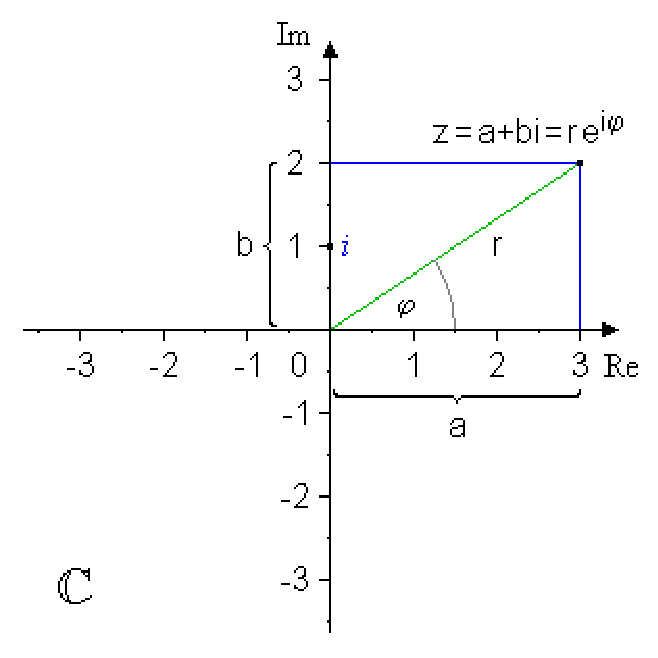
\epsfig{file=Abbildungen/gauss-ebene.eps, scale=0.7}
  \caption{Die Gau\3'sche Zahlen-Ebene.}
  \label{fig:gauss-ebene.eps}
\end{figure}

\vspace*{0.2cm}
\noindent
Bezeichnen wir den Betrag der komplexen Zahl $a + i \cdot b$ mit $r$, setzen wir also 
$r := |a + i \cdot b|$, so besteht zwischen dem in der Abbildung eingezeichneten Winkel $\varphi$
und den Komponenten $a$ und 
$b$ die Beziehung
\\[0.2cm]
\hspace*{1.3cm} $a = r \cdot \cos(\varphi)$ \quad und \quad $b = r \cdot \sin(\varphi)$.
\\[0.2cm]
Durch Division der zweiten Gleichung durch die erste Gleichung erhalten wir die Beziehung
\\[0.2cm]
\hspace*{1.3cm} $\tan(\varphi) = \bruch{b}{a}$.
\\[0.2cm]
Solange wir uns im ersten Quadranten der Ebene befinden, k\"{o}nnen wir daraus den Winkel $\varphi$ mit Hilfe
der Gleichung
\\[0.2cm]
\hspace*{1.3cm} $\varphi = \arctan\Bigl(\bruch{b}{a}\Bigr)$
\\[0.2cm]
ausrechnen.  Das Paar $\pair(r, \varphi)$ bezeichnen wir als die \colorbox{yellow}{\emph{Polarform}} der
komplexen Zahl $a + i \cdot b$, w\"{a}hrend wir das Paar $\pair(a,b)$ die \colorbox{yellow}{\emph{kartesische Darstellung}}
nennen.  Es ist instruktiv zu sehen, was passiert, wenn wir zwei
komplexe Zahlen in Polarform
\\[0.2cm]
\hspace*{1.3cm} 
$r_1 \cdot \cos(\varphi_1) + i \cdot r_1 \cdot \sin(\varphi_1)$ \quad und \quad
$r_2 \cdot \cos(\varphi_2) + i \cdot r_2 \cdot \sin(\varphi_2)$ 
\\[0.2cm]
multiplizieren.  Wir haben n\"{a}mlich
\\[0.2cm]
$
\begin{array}[t]{cl}
  & \bigl(r_1 \cdot \cos(\varphi_1) + i \cdot r_1 \cdot \sin(\varphi_1)\bigr) \cdot
    \bigl(r_2 \cdot \cos(\varphi_2) + i \cdot r_2 \cdot \sin(\varphi_2)\bigr)       \\[0.2cm]
= & r_1 \cdot r_2 \cdot
    \Bigl(\cos(\varphi_1) \cdot \cos(\varphi_2) - \sin(\varphi_1) \cdot \sin(\varphi_2) +
          i \cdot \bigl(\cos(\varphi_1) \cdot \sin(\varphi_2) + \sin(\varphi_1) \cdot \cos(\varphi_2)\bigr)
    \Bigr) \\[0.2cm]
= & r_1 \cdot r_2 \cdot
    \bigl(\cos(\varphi_1 + \varphi_2) + i \cdot \sin(\varphi_1 + \varphi_2) \bigr).
\end{array}
$
\\[0.2cm]
Im letzten Schritt dieser Umformung haben wir dabei die beiden 
\href{https://de.wikipedia.org/wiki/Formelsammlung_Trigonometrie#Additionstheoreme}{Additions-Theoreme}
\\[0.2cm]
\hspace*{1.3cm}
$\sin(\alpha + \beta) = \sin(\alpha) \cdot \cos(\beta) + \cos(\alpha) \cdot \sin(\beta)$ \quad und
\\[0.2cm]
\hspace*{1.3cm}
$\cos(\alpha + \beta) = \cos(\alpha) \cdot \cos(\beta) - \sin(\alpha) \cdot \sin(\beta)$
\\[0.2cm]
benutzt.   Wegen seiner Wichtigkeit halten wir das Ergebnis der obigen Rechnung in der folgenden Formel
fest:
\begin{equation}
  \label{eq:komplex_mult2}
  \bigl(\cos(\varphi_1) + i \cdot \sin(\varphi_1)\bigr) \cdot
  \bigl(\cos(\varphi_2) + i \cdot \sin(\varphi_2)\bigr)       
= \bigl(\cos(\varphi_1 + \varphi_2) + i \cdot \sin(\varphi_1 + \varphi_2) \bigr).
\end{equation}
Wir sehen, dass es einfach ist, komplexe Zahlen in der Polarform zu
multiplizieren: Die Winkel der Zahlen werden addiert.  Der \"{U}bersichtlichkeit halber habe ich
die Betr\"{a}ge $r_1$ und $r_2$ in der oberen Formel weggelassen.  

\subsection{Potenzen und allgemeine Wurzeln}
Ist eine komplexe Zahl in Polarform gegeben, so ist es leicht, die Zahl zu
potenzieren, denn aus Gleichung \ref{eq:komplex_mult2} folgt mit einem einfachen Induktions-Beweis,
dass f\"{u}r alle nat\"{u}rlichen Zahlen $n \in \mathbb{N}$ die Gleichung
\begin{equation}
  \label{eq:komplex_potenz}
  \bigl(\cos(\varphi) + i \cdot \sin(\varphi)\bigr)^n = \cos(n \cdot \varphi) + i \cdot \sin(n \cdot \varphi)
\end{equation}
gilt.  Diese Formel wird auch als \href{http://de.wikipedia.org/wiki/Abraham_de_Moivre}{\emph{Satz von de Moivre}} bezeichnet.  
Dieser Satz kann zum Ziehen beliebiger Wurzeln aus einer komplexen Zahl verwendet werden.  Um mit Hilfe dieses Satzes Wurzeln ziehen
zu k\"{o}nnen, bemerken wir zun\"{a}chst, dass die Funktionen $\sin(x)$ und $\cos(x)$ periodisch mit der Periode
$2 \cdot \pi$ sind, es gilt also
\\[0.2cm]
\hspace*{1.3cm}
$\sin(x + 2 \cdot \pi) = \sin(x)$ \quad und \quad
$\cos(x + 2 \cdot \pi) = \cos(x)$.
\\[0.2cm]
Diese Gleichungen lassen sich f\"{u}r beliebige $k \in \mathbb{N}$ zu
\\[0.2cm]
\hspace*{1.3cm}
$\sin(\varphi + 2 \cdot k \cdot \pi) = \sin(\varphi)$ \quad und \quad
$\cos(\varphi + 2 \cdot k \cdot \pi) = \cos(\varphi)$
\\[0.2cm]
verallgemeinern.  Wir \"{u}berlegen nun, f\"{u}r welche komplexe Zahlen der Form
\\[0.2cm]
\hspace*{1.3cm}
$z = \cos(\varphi) + i \cdot \sin(\varphi)$ \quad die Gleichung \quad $z^n = 1$
\\[0.2cm]
erf\"{u}llt ist.  Solche Zahlen bezeichnen wir als $n$-te Einheitswurzeln.  Da 
\\[0.2cm]
\hspace*{1.3cm}
$1 = \cos(2 \cdot k \cdot \pi) + i \cdot \sin(2 \cdot k \cdot \pi)$
\\[0.2cm]
gilt, muss nach Gleichung \ref{eq:komplex_potenz} f\"{u}r die Zahl $z = \cos(\varphi) + i \cdot \sin(\varphi)$
die Beziehung
\begin{equation}
  \label{eq:komplex_wurzel0}
\cos(2 \cdot k \cdot \pi) + i \cdot \sin(2 \cdot k \cdot \pi) =
\cos(n \cdot \varphi) + i \cdot \sin(n \cdot \varphi)  
\end{equation}
erf\"{u}llt sein, wenn $z^n = 1$ sein soll.  Die Gleichung \ref{eq:komplex_wurzel0} ist offensichtlich dann
erf\"{u}llt, wenn 
\\[0.2cm]
\hspace*{1.3cm}
$\varphi = \bruch{2 \cdot k \cdot \pi}{n}$
\\[0.2cm]
gilt, wobei wir $k$ auf die Elemente der Menge $\{0,1, \cdots, n-1\}$ beschr\"{a}nken k\"{o}nnen, denn gr\"{o}\3ere
Werte von $k$ liefern Winkel, die gr\"{o}\3er als $2 \cdot \pi$ sind.  Wir definieren daher
\\[0.2cm]
\hspace*{1.3cm}
\colorbox{red}{\framebox{\colorbox{blue}{\framebox{\colorbox{yellow}{
$\ds\zeta_n := \cos\Bigl(\frac{2 \cdot \pi}{n}\Bigr) + i \cdot \sin\Bigl(\frac{2 \cdot \pi}{n}\Bigr)$}}}}}
\\[0.2cm]
als die \emph{primitive} $n$-te Einheitswurzel und sehen, dass die Zahlen
\\[0.2cm]
\hspace*{1.3cm}
$\ds\zeta_n^k := \cos\Bigl(\frac{2 \cdot k \cdot \pi}{n}\Bigr) + i \cdot \sin\Bigl(\frac{2 \cdot k \cdot \pi}{n}\Bigr)$
\quad f\"{u}r $k \in \{ 0, 1, \cdots, n-1 \}$
\\[0.2cm]
dann alle $n$-ten Einheitswurzeln sind.

\example
F\"{u}r die primitive dritte Einheitswurzel $\zeta_3$ gilt
\\[0.2cm]
\hspace*{1.3cm}
$\ds\zeta_3 = \cos\Bigl(\frac{2 \cdot \pi}{3}\Bigr) + i \cdot \sin\Bigl(\frac{2 \cdot \pi}{3}\Bigr)
 = - \bruch{1}{2} + i \cdot \bruch{\sqrt{3\,}}{2}. 
$
\\[0.2cm] 
F\"{u}r $\zeta_3^2$ finden wir nach kurzer Rechnung
\\[0.2cm]
\hspace*{1.3cm}
$\ds\zeta_3^2 = \cos\Bigl(\frac{4 \cdot \pi}{3}\Bigr) + i \cdot \sin\Bigl(\frac{4 \cdot \pi}{3}\Bigr)
 = - \bruch{1}{2} - i \cdot \bruch{\sqrt{3\,}}{2}. 
$
\\[0.2cm]
Sie k\"{o}nnen leicht nachrechnen, dass sowohl $\zeta_3^3 = 1$ als auch $(\zeta_3^2)^3 = 1$ gilt.
\vspace*{0.2cm}

Mit Hilfe der $n$-ten Einheitswurzeln k\"{o}nnen wir jetzt allgemein f\"{u}r eine komplexe Zahl $z$ und eine
nat\"{u}rliche Zahl $n$ die L\"{o}sungen der Gleichung $r^n = z$ angeben.  Dazu ist zun\"{a}chst $z$ in
Polar-Koordinaten anzugeben.  Falls
\\[0.2cm]
\hspace*{1.3cm}
$z = r \cdot \bigl(\cos(\varphi) + i \cdot \sin(\varphi)\bigr)$
\\[0.2cm]
gilt, so ist offenbar f\"{u}r alle $k \in \{ 0, 1, \cdots, n - 1 \}$ die Zahl
\\[0.2cm]
\hspace*{1.3cm}
$\displaystyle s = \zeta_n^k \cdot \sqrt[n]{r\,} \cdot 
     \biggl(\cos\Bigl(\frac{\varphi}{n}\Bigr) + i \cdot \sin\Bigl(\frac{\varphi}{n}\Bigr) \biggr)
$
\\[0.2cm] 
eine L\"{o}sung der Gleichung $s^n = z$.

\example 
Wir berechnen alle L\"{o}sungen der Gleichung $r^3 = 1 + i$.  Dazu m\"{u}ssen wir zun\"{a}chst die Zahl
$1 + i$ in Polar-Koordinaten darstellen.  Setzen wir  
\\[0.2cm]
\hspace*{1.3cm} $\varphi = \arctan\Bigl(\bruch{1}{1}\Bigr) = \arctan(1) = \bruch{\pi}{4}$,
\\[0.2cm]
so gilt wegen $\sqrt{1^2 + 1^2\,} = \sqrt{2\,}$ offenbar
\\[0.2cm]
\hspace*{1.3cm} $\ds1 + i = \sqrt{2\,} \cdot \left(\cos\Bigl(\frac{\pi}{4}\Bigr) + i \cdot \sin\Bigl(\frac{\pi}{4}\Bigr)\right)$.
\\[0.2cm]
Damit erhalten wir dann als eine dritte Wurzel der Zahl $1 + i$ den Ausdruck
\\[0.2cm]
\hspace*{1.3cm}
$\ds r := \sqrt[6]{2\,} \cdot 
      \left(\cos\Bigl(\frac{\pi}{12}\Bigr) + i \cdot \sin\Bigl(\frac{\pi}{12}\Bigr)\right) 
$.
\\[0.2cm]
Ber\"{u}cksichtigen wir noch, dass die Werte der trigonometrischen Funktionen f\"{u}r das Argument
$\ds\frac{\pi}{12}$ bekannt sind, es gilt n\"{a}mlich
\\[0.2cm]
\hspace*{1.3cm} 
$\ds\cos\Bigl(\frac{\pi}{12}\Bigr) = \frac{1}{4} \cdot \bigl(\sqrt{6} + \sqrt{2}\bigr)$ \quad und \quad
$\ds\sin\Bigl(\frac{\pi}{12}\Bigr) = \frac{1}{4} \cdot \bigl(\sqrt{6} - \sqrt{2}\bigr)$,
\\[0.2cm]
so erhalten wir f\"{u}r $r$ den Ausdruck
\\[0.2cm]
\hspace*{1.3cm}
$r = \frac{1}{4} \cdot \sqrt[6]{2\,} \cdot
     \Bigl(\sqrt{6} + \sqrt{2} + i \cdot \bigl(\sqrt{6} - \sqrt{2}\bigr)\Bigr) 
$.
\\[0.2cm]
Ziehen wir hier $\sqrt{2}$ aus der Klammer und ber\"{u}cksichtigen, dass
\\[0.2cm]
\hspace*{1.3cm}
$\sqrt[6]{2} \cdot \sqrt{2} = 2^{\frac{1}{6}} \cdot 2^{\frac{1}{2}} =
 2^{\frac{4}{6}} =  2^{\frac{2}{3}} = \sqrt[3]{4}
$
\\[0.2cm]
gilt, so k\"{o}nnen wir $r$ als
\\[0.2cm]
\hspace*{1.3cm}
$r = \frac{1}{4} \cdot \sqrt[3]{4\,} \cdot \Bigl(\sqrt{3} + 1 + i \cdot \bigl(\sqrt{3} - 1\bigr)\Bigr)$
\\[0.2cm]
schreiben.  Die anderen beiden dritten Wurzeln erhalten wir daraus durch Multiplikation mit
$\zeta_3$ bzw.~$\zeta_3^2$.

\remark
Bei der obigen Rechnung hatten wir Gl\"{u}ck:  Erstens konnten wir f\"{u}r den Winkel $\varphi$ einen expliziten
Ausdruck, n\"{a}mlich $\frac{\pi}{4}$, angeben und zweitens konnten wir auch die Anwendung der trigonometrischen
Funktionen auf
\\[0.2cm]
\hspace*{1.3cm}
$\ds\frac{\varphi}{3} = \frac{\pi}{12}$ 
\\[0.2cm]
geschlossene Terme angeben.  Normalerweise
funktioniert das nicht und dann bleibt nur die numerische Rechnung. 

\exercise
Beweisen Sie, dass 
\\[0.2cm]
\hspace*{1.3cm}
$\ds\cos\Bigl(\frac{\pi}{12}\Bigr) = \frac{1}{4} \cdot \bigl(\sqrt{6} + \sqrt{2}\bigr)$ \quad und \quad
$\ds\sin\Bigl(\frac{\pi}{12}\Bigr) = \frac{1}{4} \cdot \bigl(\sqrt{6} - \sqrt{2}\bigr)$
\\[0.2cm]
gilt.  Verwenden Sie dazu den Satz von de Moivre, der im Skript als Gleichung
(\ref{eq:komplex_potenz}) angegeben ist. 
Au\3erdem d\"{u}rfen Sie in Ihrem Beweis die G\"{u}ltigkeit der Gleichungen
\\[0.2cm]
\hspace*{1.3cm}
$\ds\cos\Bigl(\frac{\pi}{6}\Bigr) = \frac{1}{2}\cdot\sqrt{3}$ \quad und \quad $\ds\sin\Bigl(\frac{\pi}{6}\Bigr) = \frac{1}{2}$
\\[0.2cm]
voraussetzen.
\exend

\section{Anwendung der komplexen Zahlen$^*$}
Wir k\"{o}nnen jetzt zwar mit komplexen Zahlen rechnen, wir haben aber bisher noch nicht gesehen, warum der 
Gebrauch von komplexen Zahlen \"{u}berhaupt notwendig ist.  Es gibt in der Mathematik eine Vielzahl von
Anwendung der komplexen Zahlen.  Stellvertretend m\"{o}chte ich an dieser Stelle die Fourier-Transformation
einer Funktion nennen, die in der Signalverarbeitung eine gro\3e Rolle spielt.  Darauf n\"{a}her einzugehen
ist aus Zeitgr\"{u}nden im Rahmen einer einf\"{u}hrenden Mathematik-Vorlesung leider unm\"{o}glich.  Auch f\"{u}r die
Anwendung komplexer Zahlen bei der L\"{o}sung von Differenzial-Gleichungen ist es jetzt noch zu fr\"{u}h.  Ich
m\"{o}chte statt dessen den historischen Weg gehen und zeigen, wie die komplexen Zahlen tats\"{a}chlich entdeckt
worden sind.  Ausgangspunkt unserer \"{U}berlegungen ist dabei die Gleichung
\\[0.2cm]
\hspace*{1.3cm}
$x^3 - 15 \cdot x - 4 = 0$.
\\[0.2cm]
Wir wollen alle m\"{o}glichen L\"{o}sungen dieser Gleichung bestimmen.  Um uns einen \"{u}berblick zu verschaffen,
skizzieren wir zun\"{a}chst die Funktion $x \mapsto x^3 - 15 \cdot x - 4$.  Wir erhalten den in Abbildung
\ref{fig:cubic.eps} auf Seite \pageref{fig:cubic.eps} gezeigten Graphen.

\begin{figure}[!ht]
  \centering
  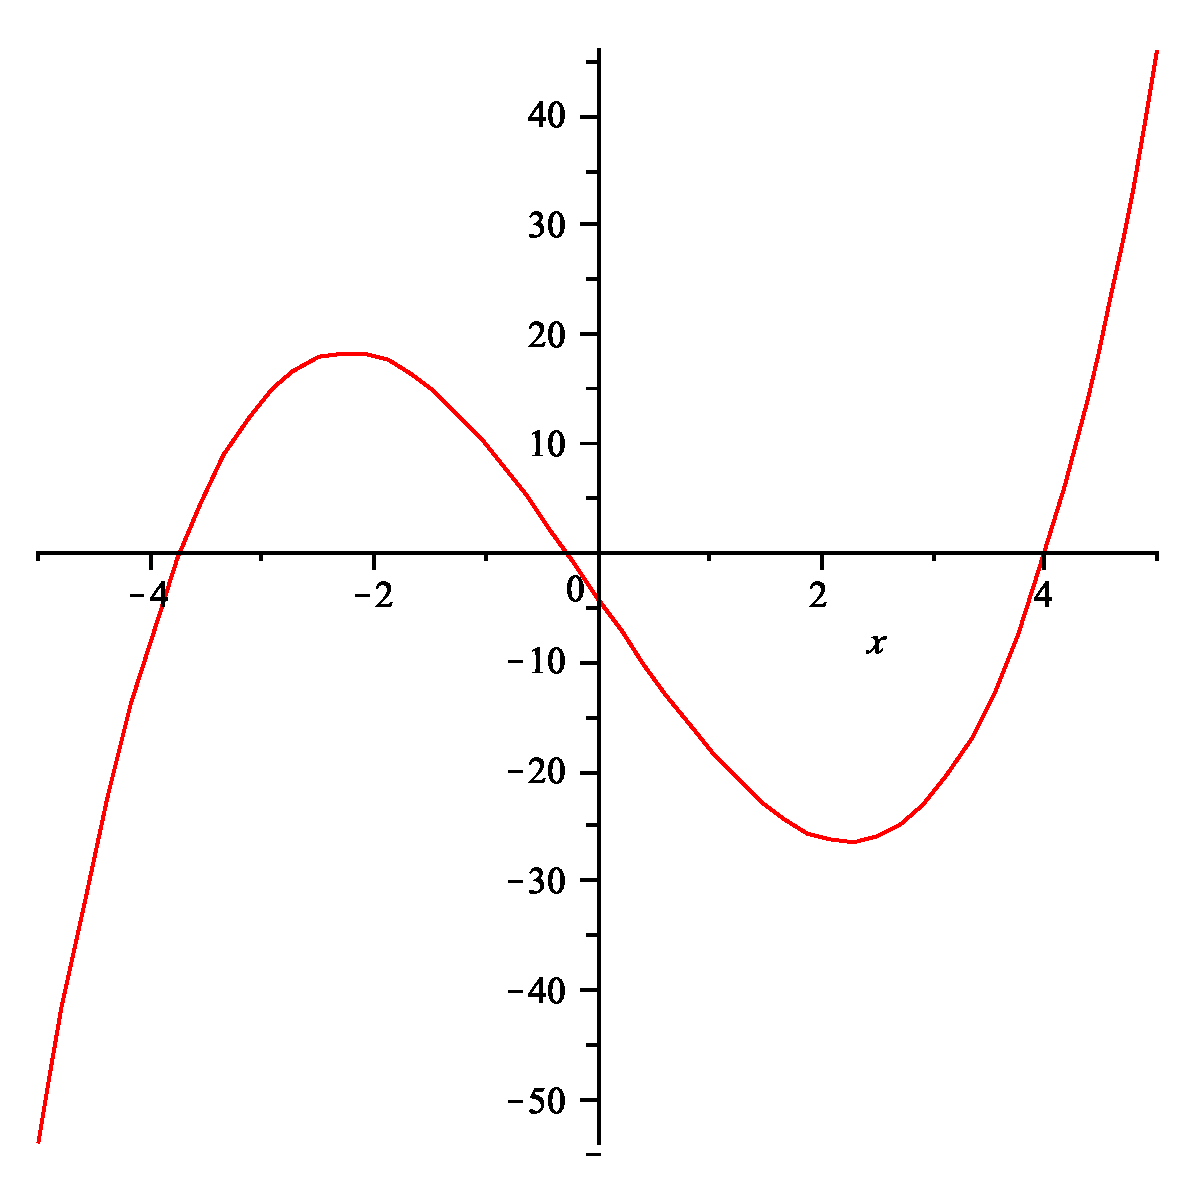
\epsfig{file=Abbildungen/cubic.eps, scale=0.4}
  \caption{Die Funktion $x \mapsto x^3 - 15 \cdot x - 4$.}
  \label{fig:cubic.eps}
\end{figure}

Es sieht so aus, als ob unsere Gleichung drei verschiedene L\"{o}sungen hat.  Um diese L\"{o}sungen zu bestimmen,
verallgemeinern wir unser Problem und versuchen, die kubische Gleichung
\begin{equation}
  \label{eq:cubic}
  x^3 - p \cdot x - q = 0  
\end{equation}
zu l\"{o}sen.  Wir machen dazu den Ansatz $x = u + v$.  Nun gilt
\\[0.2cm]
\hspace*{1.3cm}
$
\begin{array}[t]{lcl}
(u + v)^3 & = & (u + v)^2 \cdot (u + v)                                                           \\[0.2cm]
          & = & (u^2 + 2 \cdot u \cdot v + v^2) \cdot (u + v)                                     \\[0.2cm]
          & = & u^3 + u^2 \cdot v + 2 \cdot u^2 \cdot v + 2 \cdot u \cdot v^2 + u \cdot v^2 + v^3 \\[0.2cm]
          & = & u^3 + 3 \cdot u^2 \cdot v + 3 \cdot u \cdot v^2 + v^3                             \\[0.2cm]
          & = & 3 \cdot u \cdot v \cdot (u + v) + u^3 + v^3 
\end{array}
$
\\[0.2cm]
Daher k\"{o}nnen wir die kubische Gleichung mit dem Ansatz $x = u + v$ in die Gleichung
\\[0.2cm]
\hspace*{1.3cm}
$3 \cdot u \cdot v \cdot (u + v) + u^3 + v^3 - p \cdot (u + v) - q = 0$
\\[0.2cm]
\"{u}berf\"{u}hren, was wir noch zu
\\[0.2cm]
\hspace*{1.3cm}
$(3 \cdot u \cdot v - p) \cdot (u + v) + u^3 + v^3 - q = 0$
\\[0.2cm]
umschreiben.  Falls es uns gelingt, die Zahlen $u$ und $v$ so zu bestimmen, dass
\\[0.2cm]
\hspace*{1.3cm}
$p = 3 \cdot u \cdot v$ \quad und \quad $q = u^3 + v^3$
\\[0.2cm]
gilt, dann ist $x = u + v$ eine L\"{o}sung der kubischen Gleichung \ref{eq:cubic}.  Wir definieren
\\[0.2cm]
\hspace*{1.3cm}
$\alpha := u^3$ \quad und \quad $\beta := v^3$.
\\[0.2cm]
Damit lassen sich die Gleichungen f\"{u}r $u$ und $v$ umschreiben in
\\[0.2cm]
\hspace*{1.3cm}
$p^3 = 27 \cdot \alpha \cdot \beta$ \quad und \quad $q = \alpha + \beta$
\\[0.2cm]
Ist $\alpha \not= 0$, so folgt aus der ersten Gleichung
\\[0.2cm]
\hspace*{1.3cm}
$\beta = \bruch{p^3}{27 \cdot \alpha}$.
\\[0.2cm]
Setzen wir diesen Wert in die zweite Gleichung ein, so erhalten wir
\\[0.2cm]
\hspace*{1.3cm}
$q = \alpha + \bruch{p^3}{27 \cdot \alpha}$.
\\[0.2cm]
Multiplikation dieser Gleichung mit $\alpha$ liefert uns eine quadratische Gleichung f\"{u}r $\alpha$:
\\[0.2cm]
\hspace*{1.3cm}
$q \cdot \alpha = \alpha^2 + \bruch{p^3}{27}$.
\\[0.2cm]
Diese Gleichung stellen wir zu 
\\[0.2cm]
\hspace*{1.3cm}
$- \bruch{p^3}{27} = \alpha^2 - q \cdot \alpha$
\\[0.2cm]
um.  Addieren wir auf beiden Seiten die quadratische Erg\"{a}nzung $\ds\frac{q^2}{4}$, so erhalten wir
die quadratische Gleichung
\\[0.2cm]
\hspace*{1.3cm}
$\bruch{q^2}{4} - \bruch{p^3}{27} = \left(\alpha - \bruch{q}{2}\right)^2$.
\\[0.2cm]
Diese Gleichung hat offenbar die L\"{o}sung
\\[0.2cm]
\hspace*{1.3cm}
$\alpha = \bruch{q}{2} + \sqrt{\bruch{q^2}{4} - \bruch{p^3}{27}}$.
\\[0.2cm]
Wegen $q = \alpha + \beta$ folgt daraus f\"{u}r $\beta$
\\[0.2cm]
\hspace*{1.3cm}
$\beta = \bruch{q}{2} - \sqrt{\bruch{q^2}{4} - \bruch{p^3}{27}}$.
\\[0.2cm]
Wir pr\"{u}fen, ob f\"{u}r diese Werte von $\alpha$ und $\beta$ auch die zweite Bedingung 
\\[0.2cm]
\hspace*{1.3cm}
$\alpha \cdot \beta = \Bigl(\bruch{p}{3}\Bigr)^3$
\\[0.2cm]
erf\"{u}llt ist und finden tats\"{a}chlich
\\[0.2cm]
\hspace*{1.3cm}
$
\begin{array}[t]{lcl}
      \alpha \cdot \beta 
& = & \left(\bruch{q}{2} + \sqrt{\bruch{q^2}{4} - \bruch{p^3}{27}}\right) \cdot
      \left(\bruch{q}{2} - \sqrt{\bruch{q^2}{4} - \bruch{p^3}{27}}\right)        \\[0.2cm]
& = & \bruch{q^2}{4} - \left(\bruch{q^2}{4} - \bruch{p^3}{27}\right)             \\[0.2cm]
& = & \bruch{p^3}{27}.                                            
\end{array}
$
\\[0.2cm]
Ber\"{u}cksichtigen wir, dass $\alpha = u^3$, $\beta = v^3$ und $x = u + v$ ist,
so erhalten wir zur L\"{o}sung der kubischen Gleichung \ref{eq:cubic} die 
erstmals 1545 von \href{http://de.wikipedia.org/wiki/Gerolamo_Cardano}{Geralomo Cardano} ver\"{o}ffentlichte 
\emph{Cardanische Formel}
\\[0.2cm]
\hspace*{1.3cm}
\framebox{\framebox{\colorbox{amber}{
$x = \sqrt[3]{\bruch{q}{2} + \sqrt{\left(\bruch{q}{2}\right)^2 - \left(\bruch{p}{3}\right)^3\,}\;} +
     \sqrt[3]{\bruch{q}{2} - \sqrt{\left(\bruch{q}{2}\right)^2 - \left(\bruch{p}{3}\right)^3\,}\;}
$.}}}
\\[0.2cm]
In unserem urspr\"{u}nglichen Problem gilt $p = 15$ und $q = 4$.  Dann haben wir 
\\[0.2cm]
\hspace*{1.3cm}
$\alpha = \bruch{q}{2} + \sqrt{\left(\bruch{q}{2}\right)^2 - \left(\bruch{p}{3}\right)^3\,} =
 2 + \sqrt{4 - 125} = 2 + \sqrt{-121} = 2 + i \cdot 11
$.
\\[0.2cm]
Das ist aber eine komplexe Zahl, aus der wir jetzt noch die dritte Wurzel ziehen m\"{u}ssen.
An dieser Stelle haben wir Gl\"{u}ck, denn f\"{u}r die dritte Wurzel aus $2 + i \cdot 11$ und aus 
$2 - i \cdot 11$ l\"{a}sst sich jeweils ein expliziter Wert angeben, es gilt
\\[0.2cm]
\hspace*{1.3cm}
$u = \sqrt[3]{2 + i \cdot 11} = 2 + i$  \quad und \quad 
$v = \sqrt[3]{2 - i \cdot 11} = 2 - i$.
\\[0.2cm]
Wir wollen dieses Ergebnis im ersten Fall nachrechnen.  Es gilt
\\[0.2cm]
\hspace*{1.3cm}
$
\begin{array}[t]{lcl}
(2 + i)^3 & = & 2^3 + 3 \cdot 2^2 \cdot i + 3 \cdot 2 \cdot i^2 - i \\[0.2cm]
          & = & 8 - 6 + (12 - 1) \cdot i                            \\[0.2cm]
          & = & 2 + 11 \cdot i                            
\end{array}
$.
\\[0.2cm]
Damit finden wir als eine L\"{o}sung der kubischen Gleichung $x^3 - 15 \cdot x - 4 = 0$ den Wert
\\[0.2cm]
\hspace*{1.3cm}
$x_1 = 2 + 11 \cdot i + 2 - 11 \cdot i = 4$.
\\[0.2cm]
Sie sehen, dass wir ein Problem, dass mit komplexen Zahlen auf den ersten Blick nichts zu tun hat, durch die
Verwendung komplexer Zahlen l\"{o}sen konnten.
Der Vollst\"{a}ndigkeit halber wollen wir noch die anderen beiden L\"{o}sungen der kubischen Gleichung $x^3 - 15
\cdot x - 4 = 0$ bestimmen. 
Diese erhalten wir, wenn wir in der Cardanischen Formel auch die anderen M\"{o}glichkeiten f\"{u}r die dritte
Wurzel einsetzen.  Dabei m\"{u}ssen wir allerdings ber\"{u}cksichtigen, dass f\"{u}r die Zahlen $u$ und $v$ die
Nebenbedingung $3 \cdot u \cdot v = p$ gilt.  Multiplizieren wir beispielsweise $u$ mit $\zeta_3$ und 
$v$ mit $\zeta_3^2$, so haben wir
\\[0.2cm]
\hspace*{1.3cm}
$3 \cdot \zeta_3 \cdot u \cdot \zeta_3^2 \cdot v = 3 \cdot \zeta_3^3 \cdot u \cdot v = 3 \cdot u \cdot v = p$,
\\[0.2cm]
denn aus der Tatsache, dass $\zeta_3$ die dritte Einheitswurzel ist, folgt $\zeta_3^3 = 1$.  Als eine weitere L\"{o}sung erhalten wir dann
\\[0.2cm]
\hspace*{1.3cm}
$
\begin{array}[t]{lcl}
x_2 & = & \zeta_3 \cdot u + \zeta_3^2 \cdot v                               \\[0.2cm]
    & = & \zeta_3 \cdot (2 + i) + \zeta_3^2 \cdot (2 - i)                    \\[0.2cm]
    & = & \Bigl(- \bruch{1}{2} + i \cdot \bruch{\sqrt{3\,}}{2}\Bigr) \cdot (2 + i) + 
          \Bigl(- \bruch{1}{2} - i \cdot \bruch{\sqrt{3\,}}{2}\Bigr) \cdot (2 - i)   \\[0.3cm]
    & = & \bruch{1}{2} \cdot \bigl(-2 - \sqrt{3} + i \cdot (-1 + 2 \cdot \sqrt{3}) 
                                   -2 - \sqrt{3} + i \cdot ( 1 - 2 \cdot \sqrt{3})\bigr) \\[0.2cm]
    & = & - 2 - \sqrt{3}.  \\[0.2cm]
\end{array}
$
\\[0.2cm]
Auch hier ergibt sich also eine reelle L\"{o}sung.  F\"{u}r $x_3$ finden Sie nach einer \"{a}hnlichen Rechnung den Wert
\\[0.2cm]
\hspace*{1.3cm}
$x_3 = \zeta_3^2 \cdot u + \zeta_3 \cdot v = -2 + \sqrt{3}$.
\\[0.2cm]
Insgesamt zeigt dieses Beispiel, dass auch f\"{u}r Probleme, deren L\"{o}sungen reelle Zahlen sind, der Umweg
\"{u}ber die komplexen Zahlen sinnvoll sein kann.  Zum Abschluss m\"{o}chte ich noch bemerken, dass die
Verwendung komplexer Zahlen zur Bestimmung der Nullstellen eines Polynoms dritten Grades nicht
zwingend notwendig ist.  Die Nullstellen lassen sich auch auf trigonometrischem Wege bestimmen.  Dann ergibt
sich die Formel 
\\[0.2cm]
\hspace*{1.3cm}
\framebox{
\colorbox{amber}{$\ds x_{k} = 2 \cdot \sqrt{\frac{p}{3}\;} \cdot 
    \cos\left(\frac{1}{3} \cdot \arccos\Bigl(\frac{3 \cdot q}{2 \cdot p} \cdot \sqrt{\frac{3}{p}}\Bigr)
    -(k-1) \cdot \frac{2 \cdot \pi}{3}\right)$ \quad for $k = 1,2,3$.}}
\\[0.2cm]
Die trigonometrische Herleitung ist allerdings deutlich aufwendiger als die Herleitung die wir in diesem
Kapitel auf algebraischem Wege mit Hilfe der komplexen Zahlen gefunden haben.


\exercise
F\"{u}r welche $z \in \mathbb{C}$ gilt die Gleichung
\\[0.2cm]
\hspace*{1.3cm}
$\left(\bruch{1+z}{1-z}\right)^2 = -1$?
\exend

\exercise
F\"{u}r welche Zahlen $x, y \in \mathbb{R}$ gilt
\\[0.2cm]
\hspace*{1.3cm}
$(5 + 6 \cdot i) \cdot (x - 3 \cdot i) = y - 3 \cdot i$?
\exend

\exercise
Welche komplexen Zahlen $z \in \mathbb{C}$ lassen sich in der Form
\\[0.2cm]
\hspace*{1.3cm}
$\bruch{1 + i \cdot x}{1 - i \cdot x} = z$ \quad mit $x \in \mathbb{R}$
\\[0.2cm]
schreiben? 
\vspace*{0.2cm}

\noindent
\textbf{Hinweis}:  Machen Sie f\"{u}r $z$ den Ansatz $z = a + b \cdot i$ mit $a,b \in \mathbb{R}$ und
setzen Sie diesen Ansatz in der obigen Gleichung f\"{u}r $z$ ein.  
\exend

\exercise
Bestimmen Sie mit Hilfe der Cardanischen Formel alle L\"{o}sungen der Gleichung 
\\[0.2cm]
\hspace*{1.3cm}
$x^3 = 3 \cdot x - 2$!
\exend


\section{Ausblick}
In diesem letzten Abschnitt stellen wir wichtige Formeln und Eigenschaften der komplexen Zahlen
zusammen, die wir allerdings erst im zweiten Semester beweisen k\"{o}nnen.

\subsection{Die Eulersche Formel}
Zwischen der Exponential-Funktion $x \mapsto e^x$ und den trigonometrischen Funktionen 
$x \mapsto \sin(x)$ und $x \mapsto \cos(x)$ gibt es einen wichtigen Zusammenhang, der als
\colorbox{yellow}{\href{https://de.wikipedia.org/wiki/Eulersche_Formel}{Eulersche Formel}} bekannt ist.  Es gilt
\\[0.2cm]
\hspace*{1.3cm}
\colorbox{red}{\framebox{\colorbox{blue}{\framebox{\colorbox{yellow}{
$e^{i \cdot \varphi} = \cos(\varphi) + i \cdot \sin(\varphi)$.}}}}}
\\[0.2cm]
Diese Formel k\"{o}nnen wir verstehen, wenn wir die
\href{https://de.wikipedia.org/wiki/Taylorreihe}{Reihenentwicklung} der beteiligten Funktionen
kennen.  In der Analysis werden wir sp\"{a}ter sehen, dass $e^x$, $\sin(x)$ und $\cos(x)$ wie folgt als Reihen
dargestellt werden k\"{o}nnen:
\begin{enumerate}
\item $\displaystyle e^x = 1 + x + \frac{1}{2} \cdot x^2 + \frac{1}{6} \cdot x^3 + \cdots = \sum\limits_{n=0}^\infty \frac{1}{n!} \cdot x^n$,
\item $\displaystyle \sin(x) = x - \frac{1}{6} \cdot x^3 + \cdots = \sum\limits_{n=0}^\infty \frac{(-1)^{n}}{(2 \cdot n + 1)!} \cdot x^{2 \cdot n + 1}$,
\item $\displaystyle \cos(x) = 1 -  \frac{1}{2} \cdot x^2 +  \frac{1}{24} \cdot x^4 + \cdots = \sum\limits_{n=0}^\infty  \frac{(-1)^{n}}{(2 \cdot n)!} \cdot x^{2 \cdot n}$.
\end{enumerate}
Setzen wir diese Reihen in der Eulerschen Formel ein und vergleichen die Koeffizienten von $x^n$, so
k\"{o}nnen wir die G\"{u}ltigkeit der Eulerschen Formel nachvollziehen.  Setzen wir in der Eulerschen Formel
f\"{u}r $\varphi$ den Wert $\pi$ ein, so erhalten wir die \colorbox{yellow}{\emph{Eulersche Identit\"{a}t}}
\\[0.2cm]
\hspace*{1.3cm}
\colorbox{red}{\framebox{\colorbox{blue}{\framebox{\colorbox{yellow}{
$e^{i \cdot \pi} = -1$.}}}}}
\\[0.2cm]
Diese Formel liefert einen Zusammenhang zwischen $\pi$, $e$ und der imagin\"{a}ren Einheit $i$.


\subsection{Der Fundamentalsatz der Algebra}
In diesem Abschnitt zitieren wir (ohne Beweis) den sogenannten \emph{Fundamentalsatz der Algebra}.  Dieser Satz
besagt, dass jedes nicht-konstante Polynom  
\\[0.2cm]
\hspace*{1.3cm}
$p(z) = \sum\limits_{i=0}^n a_i \cdot z^i$ \quad mit $n \geq 1$ und $a_n \not=0$
\\[0.2cm]
im K\"{o}rper der komplexen Zahlen eine Nullstelle hat, d.h.~es gibt ein $z_1 \in \mathbb{C}$, so dass
$p(z_1) = 0$ ist.  Mit Hilfe der Polynom-Division k\"{o}nnen wir die Nullstelle $z_1$ aus dem Polynom $p(z)$
heraus dividieren und $p(z)$ in der Form
\\[0.2cm]
\hspace*{1.3cm}
$p(z) = (z - z_1) \cdot p_1(z)$
\\[0.2cm]
schreiben, wobei $p_1(z)$ dann ein Polynom vom Grad $n-1$ ist.  Falls $n-1 \geq 1$ ist, hat auch
$p_1(z)$ eine Nullstelle $z_2$, die wir aus $p_1(z)$ heraus dividieren k\"{o}nnen, so dass wir $p_1(z)$
in der Form
\\[0.2cm]
\hspace*{1.3cm}
$p_1(z) = (z- z_2) \cdot p_2(z)$
\\[0.2cm]
schreiben k\"{o}nnen, wobei $p_2(z)$ ein Polynom vom Grad $n-2$ ist.  Durch Iteration dieses Verfahrens
finden wir also insgesamt $n$ Zahlen $z_1, z_2, \cdots, z_n$, so dass wir $p(z)$ als das Produkt
\\[0.2cm]
\hspace*{1.3cm}
$p(z) = (z-z_1) \cdot (z-z_2) \cdot \mbox{\dots} \cdot (z-z_{n-1}) \cdot (z - z_n)$
\\[0.2cm]
schreiben k\"{o}nnen.  Dabei brauchen die komplexen Zahlen $z_i$ keineswegs paarweise verschieden zu sein,
sondern sie k\"{o}nnen auch durchaus gleich sein.  Wir bemerken noch, dass diese Darstellung bis auf die
Reihenfolge der $z_i$ eindeutig sein muss, denn die $z_i$ sind genau die Nullstellen des Polynoms
$p(z)$ und ein Polynom vom Grade $n$ hat, wie die obigen \"{U}berlegungen zeigen, h\"{o}chstens $n$
verschiedene Nullstellen.
\vspace*{0.2cm} 

\noindent
\textbf{Bemerkung}: Der Fundamentalsatz der Algebra zeigt, dass die Struktur der komplexen Zahlen
aus algebraischer Sicht wesentlich reichhaltiger als die Struktur der reellen Zahlen ist, denn in
den komplexen Zahlen hat jede Gleichung der Form
\\[0.2cm]
\hspace*{1.3cm}
$z^n + a_{n-1} \cdot z^{n-1} + \cdots + a_1 \cdot z + a_0 = 0$ \quad f\"{u}r $n \geq 1$
\\[0.2cm]
eine L\"{o}sung.  Es ist also nicht nur so, dass wir die Gleichung
\\[0.2cm]
\hspace*{1.3cm}
$z^2 + 1 = 0$
\\[0.2cm]
in den komplexen Zahlen l\"{o}sen k\"{o}nnen, sondern in den komplexen Zahlen k\"{o}nnen wir tats\"{a}chlich
j\underline{ede} quadratische Gleichung l\"{o}sen.  Dar\"{u}ber hinaus k\"{o}nnen wir auch jede kubische
Gleichung l\"{o}sen und ganz allgemein hat jede Gleichung $n$-ten Grades eine L\"{o}sung, solange $n$ nur
positiv ist.  Dies ist einer von vielen Gr\"{u}nden, warum die komplexen Zahlen so wichtig sind.
\vspace*{0.2cm}

\noindent
Der Beweis des Fundamentalsatzes der Algebra ben\"{o}tigt Hilfsmittel aus der Analysis, die wir nicht
zur Verf\"{u}gung haben.  Der Beweis ist auch nicht ganz einfach: Das k\"{o}nnen Sie beispielsweise der
Tatsache entnehmen, dass der bedeutendste Mathematiker, der je gelebt hat, 
\href{http://de.wikipedia.org/wiki/Carl_Friedrich_Gauss}{Carl Friedrich Gau\3}
diesen Satz 1799 in seiner Dissertation bewiesen hat.  Der Beweis, den Gau\3 damals gab, enthielt
allerdings noch eine L\"{u}cke.  Der erste vollst\"{a}ndige Beweis des Fundamentalsatzes der Algebra wurde 
1806 von \href{http://en.wikipedia.org/wiki/Jean-Robert_Argand}{Jean-Robert Argand} angegeben.

%%% Local Variables:  
%%% mode: latex
%%% TeX-master: "lineare-algebra"
%%% End: 
 
\chapter{Vektor-R\"{a}ume}
In diesem Kapitel werden wir zun\"{a}chst den f\"{u}r den Rest dieser Vorlesung grundlegenden
Begriff des \href{https://de.wikipedia.org/wiki/Vektorraum}{Vektor-Raums}
einf\"{u}hren.  Die Theorie der Vektor-R\"{a}ume bildet die Grundlage f\"{u}r unsere sp\"{a}tere
Behandlung \href{https://de.wikipedia.org/wiki/Lineares_Gleichungssystem}{linearer Gleichungs-Systeme}. 
Au\3erdem ben\"{o}tigen wir Vektor-R\"{a}ume bei der L\"{o}sung von
\href{https://en.wikipedia.org/wiki/Recurrence_relation}{Rekurrenz-Gleichungen}, die wir im letzten  
Kapitel dieses Skriptes diskutieren.  Daneben gibt es zahlreiche weitere Anwendungen von Vektor-R\"{a}umen in der
Informatik.  Diese alle aufzulisten w\"{u}rde Ihnen jetzt wenig helfen, wir beginnen statt dessen mit
der Definition. 

\renewcommand{\labelenumi}{\arabic{enumi}.}
\renewcommand{\labelenumii}{(\alph{enumii})}

\section{Definition und Beispiele}
\begin{Definition}[Vektor-Raum]
Ein Paar $\mathcal{V} = \bigl\langle \langle V, \vec{0}, + \rangle, \cdot \bigr\rangle$ ist ein
\colorbox{yellow}{\emph{$\mathbb{K}$-Vektor-Raum}} falls gilt:
\begin{enumerate}
\item $\mathbb{K}$ ist ein K\"{o}rper.  

      In allen Beispielen, die uns in dieser Vorlesung begegnen werden,
      ist $\mathbb{K}$ entweder der K\"{o}rper der reellen Zahlen $\mathbb{R}$ oder der K\"{o}rper der komplexen Zahlen $\mathbb{C}$. 
\item $\langle V, \vec{0}, + \rangle$ ist eine kommutative Gruppe.
\item $\cdot: \mathbb{K} \times V \rightarrow V$ ist eine Abbildung, die jeder Zahl $\lambda \in \mathbb{K}$ und jedem 
      $\vec{x} \in V$ ein Element $\lambda \cdot \vec{x} \in V$ zuordnet. 
      Diese Funktion  wird als \colorbox{yellow}{\emph{Skalar-Multiplikation}} bezeichnet und
      \"{u}blicherweise in Infix-Notation geschrieben. 

      Die Skalar-Multiplikation muss au\3erdem den folgenden Gesetzen gen\"{u}gen:
      \begin{enumerate}
      \item $(\alpha \cdot \beta)  \cdot \vec{x} =  \alpha \cdot (\beta \cdot \vec{x})$ \quad f.a.  $\alpha,\beta \in \mathbb{K}$,  $\vec{x} \in V$.

            Beachten Sie, dass der Operator ``$\cdot$'', der hier in dem Ausdruck $(\alpha \cdot \beta)$ auftritt, 
            die Multiplikation in dem K\"{o}rper $\mathbb{K}$ bezeichnet, w\"{a}hrend alle anderen Auftreten des Operators ``$\cdot$'' 
            die Skalar-Multiplikation bezeichnen.  

            Dieses Gesetz wird als das \colorbox{yellow}{\emph{Assoziativ-Gesetz}} bezeichnet.  Es dr\"{u}ckt
            aus, dass die Multiplikation in dem K\"{o}rper $\mathbb{K}$ mit der Skalar-Multiplikation
            vertr\"{a}glich ist.
      \item $(\alpha + \beta) \cdot \vec{x} = \alpha \cdot \vec{x} + \beta \cdot \vec{x}$ \quad f.a.  $\alpha,\beta \in \mathbb{K}$,  $\vec{x} \in V$.

            Beachten Sie, dass der Operator ``$+$'', der  hier in dem Ausdruck $(\alpha + \beta)$
            auftritt, die Addition in dem K\"{o}rper $\mathbb{K}$ bezeichnet, w\"{a}hrend der
            Operator ``$+$'' in dem Ausdruck auf der rechten Seite dieser Gleichung die 
            Addition in der Gruppe $\langle V, \vec{0}, + \rangle$ bezeichnet.  
      \item $\alpha \cdot (\vec{x} + \vec{y}) = \alpha \cdot \vec{x} + \alpha \cdot \vec{y}$ \quad f.a. $\alpha \in \mathbb{K}$,  $\vec{x}, \vec{y} \in V$.

            Die letzten beiden Gesetze werden als \colorbox{yellow}{\emph{Distributiv-Gesetze}}
            bezeichnet.  Sie zeigen, inwiefern die Skalar-Multiplikation mit der Addition im Vektor-Raum
            $\mathcal{V}$ und der Addition im K\"{o}rper $\mathbb{K}$ vertr\"{a}glich ist.
      \item $1 \cdot \vec{x} = \vec{x}$ \quad f.a. $\vec{x} \in V$.  

            Dieses Gesetz dr\"{u}ckt aus, dass das neutrale Element der Multiplikation des K\"{o}rpers
            $\mathbb{K}$ auch bez\"{u}glich der Skalar-Multiplikation ein neutrales Element ist. 
      \end{enumerate}
\end{enumerate} 
Ist $\mathcal{V} = \bigl\langle \langle V, \vec{0}, + \rangle, \cdot \bigr\rangle$  ein $\mathbb{K}$-Vektor-Raum, so bezeichnen wir die Elemente der Menge
$V$ als \colorbox{yellow}{\emph{Vektoren}}, w\"{a}hrend die Elemente aus dem K\"{o}rper $\mathbb{K}$ 
\colorbox{yellow}{\emph{Skalare}} genannt werden.  Den K\"{o}rper $\mathbb{K}$ nennen wir den
\colorbox{yellow}{\emph{Skalaren-K\"{o}rper}} des Vektor-Raums $\mathcal{V}$.  
\eoxs
\end{Definition}

\remark
Es ist in der Literatur \"{u}blich, Vektoren von Skalaren durch Fettdruck zu unterscheiden.  
Da aber an der Tafel ein Fettdruck kaum m\"{o}glich ist, habe ich mich dazu entschlosen, 
Vektoren durch Pfeilen zu kennzeichnen.
\eoxs


\example
F\"{u}r eine Menge $K$ haben wir die Menge $K^n$ als die Menge aller Listen der L\"{a}nge $n$ definiert,
deren Elemente aus der Menge $K$ stammen.  Ist nun $\mathbb{K} = \langle K, 0, 1, +, \cdot\rangle$
ein K\"{o}rper, so definieren wir zun\"{a}chst
\\[0.2cm]
\hspace*{1.3cm}
$\vec{0} := \underbrace{[0, \cdots, 0]}_n$ .
\\[0.2cm]
Anschlie�end definieren wir eine Addition ``${\color{blue}{+}}$'' auf $K^n$ komponentenweise durch
\\[0.2cm]
\hspace*{1.3cm}
$[x_1, \cdots, x_n] {\color{blue}{+}} [y_1, \cdots, y_n] := [x_1 + y_1, \cdots, x_n + y_n]$,
\\[0.2cm]
so k\"{o}nnen Sie nachrechnen, dass mit diesen Definitionen das Tripel
\\[0.2cm]
\hspace*{1.3cm}
$\langle \mathbb{K}^n, \vec{0}, +\rangle$
\\[0.2cm]
eine kommutative Gruppe ist.  Definieren wir weiter die Skalar-Multiplikation
${\color{blue}\cdot}$ durch
\\[0.2cm]
\hspace*{1.3cm}
$\alpha {\color{blue}{\cdot}} [x_1, \cdots, x_n] := [\alpha \cdot x_1, \cdots, \alpha \cdot x_n]$,
\\[0.2cm]
wobei in den Ausdr\"{u}cken $\alpha \cdot x_i$ der Operator ``$\cdot$'' die Multiplikation in dem K\"{o}rper $\mathbb{K}$ bezeichnet,
dann l\"{a}sst sich mit etwas Rechenaufwand einsehen, dass das Paar
\\[0.2cm]
\hspace*{1.3cm}
$\mathbb{K}^n := \bigl\langle \langle K^n, \vec{0}, {\color{blue}{+}} \rangle, {\color{blue}{\cdot}} \bigr\rangle$ 
\\[0.2cm]
ein $\mathbb{K}$-Vektor-Raum ist.  Der K\"{u}rze halber werden wir in Zukunft einfach von $\mathbb{K}^n$ als Vektor-Raum reden, wobei wir dann in Wahrheit das obige Paar meinen. 
\eox

\exercise
Beweisen Sie, dass die oben definierte Struktur $\mathbb{K}^n$ f\"{u}r einen beliebigen K\"{o}rper
$\mathbb{K}$ ein $\mathbb{K}$-Vektor-Raum ist. \eox 


Der Begriff des Vektor-Raums versucht, die algebraische Struktur der Menge $\mathbb{K}^n$
axiomatisch zu erfassen.  Das ist deswegen n\"{u}tzlich, weil es neben dem Vektor-Raum 
$\mathbb{K}^n$ noch viele andere Beispiele gibt, welche dieselbe algebraische
Struktur wie der Vektor-Raum $\mathbb{K}^n$ aufweisen.  


\example
Die Menge $\mathbb{R}^{\mathbb{R}}$ ist die Menge der Funktionen der Form
\\[0.2cm]
\hspace*{1.3cm}
 $f: \mathbb{R} \rightarrow \mathbb{R}$,
\\[0.2cm]
also die Menge aller Funktionen von $\mathbb{R}$ nach $\mathbb{R}$.
Definieren wir die Addition zweier Funktionen punktweise, definieren wir f\"{u}r $f,g \in \mathbb{R}^{\mathbb{R}}$ also die
Funktion $f+g$ indem wir
\\[0.2cm]
\hspace*{1.3cm}
$(f+g)(x) := f(x) + g(x)$  \quad f.a. $x \in \mathbb{R}$
\\[0.2cm]
setzen, so ist die so definierte Funktion $f + g$ wieder eine Funktion von
$\mathbb{R}$ nach $\mathbb{R}$.  F\"{u}r ein $\alpha \in \mathbb{R}$ und $f
\in\mathbb{R}^{\mathbb{R}}$ definieren wir die Funktion
$\alpha {\color{blue}{\cdot}} f$ als
\\[0.2cm]
\hspace*{1.3cm}
$(\alpha {\color{blue}{\cdot}} f)(x) := \alpha \cdot f(x)$ \quad f.a. $x \in \mathbb{R}$.
\\[0.2cm]
Dann ist auch  $\alpha {\color{blue}{\cdot}} f$ eine Funktion von $\mathbb{R}$ nach $\mathbb{R}$.  
Schlie\3lich definieren wir eine Funktion
 $\vec{0}:\mathbb{R} \rightarrow \mathbb{R}$, indem wir
\\[0.2cm]
\hspace*{1.3cm}
$\vec{0}(x) := 0$ \quad f.a. $x \in \mathbb{R}$ 
\\[0.2cm]
setzen.  Offensichtlich  gilt $\vec{0} \in \mathbb{R}^{\mathbb{R}}$.  Nun k\"{o}nnen Sie
in einer zwar l\"{a}nglichen, aber geradlinigen Rechnung nachpr\"{u}fen, dass die so definierte Struktur
\\[0.2cm]
\hspace*{1.3cm}
$\bigl\langle \langle \mathbb{R}^{\mathbb{R}}, \vec{0}, + \rangle, \cdot \bigr\rangle$
\\[0.2cm]
ein Vektor-Raum ist.  Das folgt letzlich daraus, dass das Assoziativ-Gesetz und das Distributiv-Gesetz f\"{u}r reelle Zahlen
gilt.
 \eoxs

\example
Es sei $\mathbb{K} = \langle K, 0,1,+,\cdot\rangle$ ein K\"{o}rper.  Dann definieren wir $K^\mathbb{N}$ als den Raum aller
Folgen mit Elementen aus $K$.  Definieren wir f\"{u}r zwei
Folgen
$\bigl(x_n\bigr)_{n\in\mathbb{N}}$ und $\bigl(y_n\bigr)_{n\in\mathbb{N}}$ die Summe durch
\\[0.2cm]
\hspace*{1.3cm}
$\bigl(x_n\bigr)_{n\in\mathbb{N}} {\color{blue}{+}} \bigl(y_n\bigr)_{n\in\mathbb{N}} := \bigl(x_n + y_n\bigr)_{n\in\mathbb{N}}$ 
\\[0.2cm]
und die Skalar-Multiplikation durch
\\[0.2cm]
\hspace*{1.3cm}
$\alpha {\color{blue}{\cdot}} \bigl(x_n\bigr)_{n\in\mathbb{N}} := \bigl(\alpha \cdot x_n \bigr)_{n\in\mathbb{N}}$
\\[0.2cm]
und definieren wir $\vec{0}$ als die Folge $(0)_{n\in\mathbb{N}}$, also als die Folge,
deren s\"{a}mtliche Glieder den Wert $0$ haben, so l\"{a}sst sich zeigen, dass die Struktur
 $\bigl\langle\langle K^\mathbb{N}, \vec{0}, {\color{blue}{+}}\rangle, {\color{blue}{\cdot}}\rangle$  ein Vektor-Raum ist.
\eox


\exercise
Es sei $\bigl\langle \langle V, 0, +\rangle, \cdot\bigr\rangle$ ein $\mathbb{K}$-Vektor-Raum.  Beweisen Sie:
\renewcommand{\labelenumi}{(\alph{enumi})}
\begin{enumerate}
\item $0 \cdot \vec{x} = \vec{0}$ \quad f.a. $\vec{x} \in V$,
\item $\forall \alpha \in \mathbb{K}: \forall \vec{x} \in V: \bigl(\alpha \cdot \vec{x} = \vec{0} \rightarrow \alpha = 0 \vee \vec{x} = 0\bigr)$,
\item $(-1) \cdot \vec{x} = -\vec{x}$ \quad f.a. $\vec{x} \in V$,

      wobei hier mit $-\vec{x}$ das additive Inverse von $x$ in der Gruppe $\langle V, \vec{0}, +\rangle$
      bezeichnet wird. 
      \eoxs
\end{enumerate}
\renewcommand{\labelenumi}{\arabic{enumi}.}

\section{Basis und Dimension}
In diesem Abschnitt f\"{u}hren wir den f\"{u}r die Theorie der Vektor-R\"{a}ume zentralen Begriff
der \colorbox{yellow}{\emph{Dimension}}
ein.  Dazu definieren wir zun\"{a}chst, was wir unter einem \colorbox{yellow}{\emph{Erzeugenden-System}}
verstehen und wann eine Menge von Vektoren \colorbox{yellow}{\emph{linear unabh\"{a}ngig}} ist.

\begin{Definition}[Linear-Kombination] \lb
Es sei $\mathcal{V} = \bigl\langle \langle V, \vec{0}, + \rangle, \cdot \bigr\rangle$ ein $\mathbb{K}$-Vektor-Raum.  Ein Vektor $\vec{x} \in V$ ist eine
\colorbox{yellow}{\emph{Linear-Kombination}} der Vektoren $\vec{y}_1, \cdots, \vec{y}_n \in V$ genau dann, wenn es Skalare
$\alpha_1, \cdots, \alpha_n \in \mathbb{K}$ gibt, so dass die Gleichung
\\[0.2cm]
\hspace*{1.3cm}
$\vec{x} = \alpha_1 \cdot \vec{y}_1 + \cdots + \alpha_n \cdot \vec{y}_n$
\\[0.2cm]
gilt.  
\colorbox{red}{Zus\"{a}tzlich m\"{u}ssen die Vektoren $\vec{y}_i$ alle paarweise verschieden sein.}
Die obige Gleichung werden wir in Zukunft der K\"{u}rze halber gelegentlich auch in der Form
\\[0.2cm]
\hspace*{1.3cm}
$\vec{x} = \sum\limits_{i=1}^n \alpha_i \cdot \vec{y}_i$
\\[0.2cm]
schreiben.
\eoxs
\end{Definition}

\example
Definieren wir
\\[0.2cm]
\hspace*{1.3cm}
$\vec{y}_1 := [1, 0, 2]$, \quad  $\vec{y}_2 := [1, 2, 0]$, \quad  $\vec{y}_3 := [0, -1, 3]$  \quad und \quad  $\vec{x} := [3, 1, 11]$,
\\[0.2cm]
so ist $\vec{x}$ eine Linear-Kombination der Vektoren $\vec{y}_1$, $\vec{y}_2$, $\vec{y}_3$, denn es gilt
\\[0.2cm]
\hspace*{1.3cm}
$\vec{x} = 1 \cdot \vec{y}_1 + 2 \cdot \vec{y}_2 + 3 \cdot \vec{y}_3$.  \eoxs

\begin{Definition}[linear unabh\"{a}ngig] \lb
Es sei $\mathcal{V} = \bigl\langle \langle V, \vec{0}, + \rangle, \cdot \bigr\rangle$ ein $\mathbb{K}$-Vektor-Raum.  
Eine Menge $B \subseteq V$ ist \colorbox{yellow}{\emph{linear unabh\"{a}ngig}} genau dann, wenn 
f\"{u}r jede endliche Teilmenge
\\[0.2cm]
\hspace*{1.3cm}
$\bigl\{ \vec{x}_1, \cdots, \vec{x}_n \bigr\} \subseteq B$,
\\[0.2cm]
\colorbox{red}{bei der die Vektoren $\vec{x}_i$ paarweise verschieden sind,} die Formel
\\[0.2cm]
\hspace*{1.3cm}
$\sum\limits_{i=1}^n \alpha_i \cdot \vec{x}_i = \vec{0} \;\Rightarrow\; \forall i \in \{1,\cdots,n\}: \alpha_i = 0$
\\[0.2cm]
gilt.  Mit anderen Worten:  Der Nullvektor $\vec{0}$ l\"{a}sst sich nur als die sogenannte
\colorbox{yellow}{\emph{triviale Linear-Kombination}} aus Vektoren der Menge $B$ darstellen.  Demgegen\"{u}ber hei\3t eine
Menge $B \subseteq V$ \colorbox{yellow}{\emph{linear abh\"{a}ngig}} genau dann, wenn $B$ nicht linear unabh\"{a}ngig ist.  In
diesem Fall gibt es dann Vektoren $\vec{x}_1$, $\cdots$, $\vec{x}_n \in B$, die paarweise
verschieden sind, sowie Skalare $\alpha_1,\cdots,\alpha_n \in \mathbb{K}$, so dass einerseits
\\[0.2cm]
\hspace*{1.3cm}
$\sum\limits_{i=1}^n \alpha_i \cdot \vec{x}_i = \vec{0}$, \quad aber andererseits auch \quad
$\exists i \in \{1,\cdots,n\}: \alpha_i \,\not=\, 0$
\\[0.2cm]
gilt.  
\eoxs
\end{Definition}

\example
Definieren wir
\\[0.2cm]
\hspace*{1.3cm}
$\vec{y}_1 := [1, 0, 2]$, \quad  $\vec{y}_2 := [1, 2, 0]$ \quad und \quad $\vec{y}_3 := [0, -1, 3]$,
\\[0.2cm]
so ist die Menge $B := \{ \vec{y}_1, \vec{y}_2, \vec{y}_3 \}$
linear unabh\"{a}ngig.  Zum Beweis dieser Behauptung nehmen wir zun\"{a}chst an, dass es $\alpha_1$,
$\alpha_2$ und $\alpha_3$, gibt, so dass
\\[0.2cm]
\hspace*{1.3cm}
$\vec{0} = \alpha_1 \cdot [1,0,2] + \alpha_2 \cdot [1,2,0] + \alpha_3 \cdot [0,-1,3]$
\\[0.2cm]
gilt.  Ersetzen wir $\vec{0}$ durch die Liste $[0,0,0]$ und rechnen die rechte Seite
dieser Gleichung aus, so erhalten wir die Gleichung
\\[0.2cm]
\hspace*{1.3cm}
$[0,0,0] = [\alpha_1  + \alpha_2, 2 \cdot \alpha_2 - \alpha_3, 2 \cdot \alpha_1 + 3 \cdot \alpha_3]$.
\\[0.2cm]
Die drei Komponenten der Vektoren auf der linken und der rechten Seite dieser Gleichung m\"{u}ssen
gleich sein.  Damit m\"{u}ssen die drei Gleichungen
\\[0.2cm]
\hspace*{1.3cm}
$0 = \alpha_1 + \alpha_2$, \quad $0 = 2 \cdot \alpha_2 - \alpha_3$ \quad und \quad $0 = 2 \cdot \alpha_1 + 3 \cdot \alpha_3$
\\[0.2cm]
gelten.  Aus der zweiten Gleichung folgt nun $\alpha_3 = 2 \cdot \alpha_2$, w\"{a}hrend aus der ersten
Gleichung $\alpha_1 = - \alpha_2$ folgt.  Ersetzen wir nun in der letzten Gleichung 
$\alpha_1$ durch $-\alpha_2$ und $\alpha_3$ durch $2 \cdot \alpha_2$, so erhalten wir die neue Gleichung
\\[0.2cm]
\hspace*{1.3cm}
$0 = 2 \cdot (- \alpha_2) + 3 \cdot 2 \cdot \alpha_2$,
\\[0.2cm]
die wir auch als $0 = 4 \cdot \alpha_2$ schreiben k\"{o}nnen.  Daraus folgt aber sofort $\alpha_2 = 0$
und das impliziert dann auch $\alpha_1 = 0$ und $\alpha_3 = 0$.  Damit haben wir gezeigt, dass die drei
Vektoren $\vec{y}_1$, $\vec{y}_2$, $\vec{y}_3$ sich nur trivial zu dem Null-Vektor
$\vec{0}$ kombinieren lassen.  Folglich ist die Menge $B$ linear unabh\"{a}ngig.
\eox

\begin{Definition}[Erzeugenden-System]
  Es sei $\mathcal{V} = \bigl\langle \langle V, \vec{0}, + \rangle, \cdot \bigr\rangle$ ein $\mathbb{K}$-Vektor-Raum 
  und $B \subseteq V$.  Die Teilmenge $B$ ist ein
  \colorbox{yellow}{\emph{Erzeugenden-System}} des Vektor-Raums $\mathcal{V}$ genau dann, wenn sich jeder Vektor 
  $\vec{x} \in V$ als Linear-Kombination von Vektoren aus $B$ schreiben l\"{a}sst. 
  Als Formel schreibt sich dies wie folgt:
  \\[0.2cm]
  \hspace*{1.3cm}
  $\forall \vec{x} \in V: \exists n \in \mathbb{N}: \exists  \vec{y}_1, \cdots,
  \vec{y}_n \in B: \exists \alpha_1, \cdots, \alpha_n \in \mathbb{K}: 
  \vec{x} = \sum\limits_{i=1}^n \alpha_i \cdot \vec{y}_i
  $. \eoxs
\end{Definition}

F\"{u}r jeden Vektor-Raum $\mathcal{V} = \bigl\langle \langle V, \vec{0}, + \rangle, \cdot \bigr\rangle$ 
gibt es ein triviales Erzeugenden-System, denn nat\"{u}rlich ist die gesamte 
Menge $V$ ein Erzeugenden-System von $\mathcal{V}$.  Um das einzusehen, setzen wir f\"{u}r einen gegebenen Vektor
$\vec{x} \in V$ in der obigen Definition $n:=1$, $\vec{y}_1 := \vec{x}$ und $\alpha_1 := 1$
und haben dann trivialerweise
\\[0.2cm]
\hspace*{1.3cm}
$\vec{x} = 1 \cdot \vec{x} = 1 \cdot \vec{y}_1$,
\\[0.2cm]
womit $\vec{x}$ als Linear-Kombination von Elementen der Menge $V$ dargestellt ist.  Aber
nat\"{u}rlich ist ein solches Erzeugenden-System nicht sonderlich interessant.  Interessanter sind
Erzeugenden-Systeme, die m\"{o}glichst wenige Elemente haben, die also bez\"{u}glich der Anzahl
der Elemente \emph{minimal} sind.  Dies f\"{u}hrt zu der folgenden zentralen Definition.

\begin{Definition}[Basis]
  Es sei $\mathcal{V} = \bigl\langle \langle V, \vec{0}, + \rangle, \cdot \bigr\rangle$ ein $\mathbb{K}$-Vektor-Raum 
  und $B \subseteq V$.  Die Teilmenge $B$ ist eine
  \colorbox{yellow}{\emph{Basis}} von $V$, wenn das Folgende gilt:
  \begin{enumerate}
  \item $B$ ist ein Erzeugenden-System von $V$ und
  \item $B$ ist linear unabh\"{a}ngig.  \eoxs
  \end{enumerate}
\end{Definition}

\noindent
Der n\"{a}chste Satz zeigt, dass eine Basis eine \colorbox{red}{maximale} Menge linear unabh\"{a}ngiger Vektoren ist.

\begin{Satz}
  Es sei $\mathcal{V} = \bigl\langle \langle V, \vec{0}, + \rangle, \cdot \bigr\rangle$ 
  ein $\mathbb{K}$-Vektor-Raum und $B$ sei eine Basis von $\mathcal{V}$.  Ist $\vec{x} \in V \backslash B$,
  so ist die Menge $B \cup \{ \vec{x} \}$ linear abh\"{a}ngig.
\end{Satz}

\proof
Da $B$ eine Basis ist, ist $B$ insbesondere auch ein Erzeugenden-System von $\mathcal{V}$.  Damit gibt es ein
$n \in \mathbb{N}$ und Vektoren $\vec{y}_1,\cdots,\vec{y}_n \in B$ sowie Skalare $\alpha_1, \cdots,\alpha_n \in \mathbb{K}$,
so dass
\\[0.2cm]
\hspace*{1.3cm}
$\vec{x} = \alpha_1 \cdot \vec{y}_1 + \cdots + \alpha_n \cdot \vec{y}_n$
\\[0.2cm]
gilt.  O.B.d.A. k\"{o}nnen wir hier davon ausgehen, dass die Vektoren $\vec{y}_i$ paarweise
verschieden sind, denn wenn f\"{u}r $i\not= j$ die Gleichung $\vec{y}_i = \vec{y}_j$
gelten sollte, so k\"{o}nnen wir den Vektor $\vec{y}_j$ in der obigen Summe fallen lassen,
indem wir $\alpha_i$ durch $\alpha_i + \alpha_j$ ersetzen.

Stellen wir die obige Gleichung f\"{u}r $\vec{x}$ zu der Gleichung
\\[0.2cm]
\hspace*{1.3cm}
$\vec{0} = (-1) \cdot \vec{x} + \alpha_1 \cdot \vec{y}_1 + \cdots + \alpha_n \cdot \vec{y}_n$
\\[0.2cm]
um, so haben wir eine nicht-triviale Linear-Kombination des Null-Vektors aus Vektoren der Menge 
$B \cup \{ \vec{x} \}$ gefunden.  Dies zeigt, dass die Menge $B \cup \{ \vec{x} \}$ linear abh\"{a}ngig
ist. \qeds

\exercise
\"{U}berlegen Sie, an welcher Stelle die Voraussetzung $\vec{x} \not\in B$ in dem obigen Beweis benutzt wird!
\eox

\noindent
Der letzte Satz l\"{a}sst sich in dem folgenden Sinne umkehren.

\begin{Satz}
  Es sei $\mathcal{V} = \bigl\langle \langle V, \vec{0}, + \rangle, \cdot \bigr\rangle$ ein $\mathbb{K}$-Vektor-Raum 
  und $B \subseteq V$.  Falls $B$ eine \emph{maximale} linear 
  unabh\"{a}ngige Teilmenge von $V$ ist, falls also gilt:
  \begin{enumerate}
  \item $B$ ist linear unabh\"{a}ngig und
  \item f\"{u}r alle Vektoren $\vec{x} \in V \backslash B$ ist die Menge $B \cup \{ \vec{x} \}$
        linear abh\"{a}ngig,
  \end{enumerate}
  dann ist $B$ schon eine Basis von $V$.
\end{Satz}

\proof
Wir m\"{u}ssen nur noch zeigen, dass $B$ ein Erzeugenden-System von $\mathcal{V}$ ist.  Dazu ist nachzuweisen,
dass sich jeder Vektor $\vec{x} \in V$ als Linear-Kombination von Vektoren aus $B$ schreiben
l\"{a}sst.  Wir unterscheiden zwei F\"{a}lle:
\begin{enumerate}
\item $\vec{x} \in B$.

      In diesem Fall setzen wir $n := 1$, $\vec{y}_1 := \vec{x}$ und $\alpha_1 := 1$.  Damit
      gilt offenbar
      \\[0.2cm]
      \hspace*{1.3cm}
      $\vec{x} = \alpha_1 \cdot \vec{y}_1$
      \\[0.2cm]
      und wir haben die gesuchte Linear-Kombination gefunden.
\item $\vec{x} \not\in B$.

      Nach Voraussetzung ist die Menge $B \cup \{ \vec{x} \}$ linear abh\"{a}ngig.  Damit l\"{a}sst sich
      der Null-Vektor als nicht-triviale Linear-Kombination von Vektoren aus $B \cup \{\vec{x}\}$
      schreiben.  Nun gibt es zwei M\"{o}glichkeiten:
      \begin{enumerate}
      \item Der Vektor $\vec{x}$ wird bei dieser Linear-Kombination gar nicht ben\"{o}tigt.
            Dann h\"{a}tten wir aber eine nicht-triviale Linear-Kombination des Null-Vektors aus
            Vektoren der Menge $B$.  Da die Menge $B$ nach Voraussetzung linear unabh\"{a}ngig ist,
            kann dieser Fall nicht eintreten.
      \item Der Vektor $\vec{x}$ tritt in der nicht-trivialen Linear-Kombination des
            Null-Vektors auf.  Es gibt dann ein $n \in \mathbb{N}$, sowie Vektoren $\vec{y}_1,
            \cdots, \vec{y}_n$ und Skalare $\alpha_1, \cdots, \alpha_n, \alpha_{n+1}$,
            so dass 
            \\[0.2cm]
            \hspace*{1.3cm}
            $\vec{0} = \alpha_1 \cdot \vec{y}_1 + \cdots + \alpha_n \cdot \vec{y}_n + \alpha_{n+1} \cdot \vec{x}$
            \\[0.2cm]
            gilt.  Hierbei muss $\alpha_{n+1} \not=0$ gelten, denn sonst w\"{u}rde $\vec{x}$ in der
            Linear-Kombination gar nicht ben\"{o}tigt und diesen Fall haben wir ja bereits
            ausgeschlossen.  Damit 
            k\"{o}nnen wir die obige Gleichung zu
            \\[0.2cm]
            \hspace*{1.3cm}
            $\vec{x} = -\bruch{\alpha_1}{\alpha_{n+1}} \cdot \vec{y}_1 - \cdots - \bruch{\alpha_n}{\alpha_{n+1}} \cdot \vec{y}_n$
            \\[0.2cm] 
            umstellen.  Diese Gleichung zeigt, dass $\vec{x}$ sich als Linear-Kombination von Vektoren aus
            $B$ schreiben l\"{a}sst und das war zu zeigen. 
      \end{enumerate}
\end{enumerate}
Insgesamt haben wir jetzt gezeigt, dass sich jeder Vektor $\vec{x}\in V$ als Linear-Kombination
von Vektoren aus $B$ schreiben l\"{a}sst und damit ist $B$ ein Erzeugenden-System von $V$.  \qed

Die letzten beiden S\"{a}tze lassen sich dahingehen zusammenfassen, dass eine Menge
$B \subseteq V$ genau dann eine Basis von $V$ ist, wenn $B$ eine maximale linear unabh\"{a}ngige
Teilmenge von $V$ ist.  Die n\"{a}chsten beide S\"{a}tze zeigen, dass sich eine Basis auch als minimales
Erzeugenden-System charakterisieren l\"{a}sst.

\begin{Satz}
  Es sei $\mathcal{V} = \bigl\langle \langle V, \vec{0}, + \rangle, \cdot \bigr\rangle$ ein
  $\mathbb{K}$-Vektor-Raum und $B$ sei eine Basis von $\mathcal{V}$.  Ist $\vec{x} \in B$,
  so ist die Menge $B \backslash \{ \vec{x} \}$ kein Erzeugenden-System von $\mathcal{V}$.
\end{Satz}

\proof
Wir f\"{u}hren den Beweis indirekt und nehmen an, dass die Menge $B \backslash \{ \vec{x} \}$ ein 
Erzeugenden-System von $\mathcal{V}$ ist.  Dann m\"{u}sste sich insbesondere auch der Vektor $\vec{x}$ als
Linear-Kombination von Vektoren aus  $B \backslash \{ \vec{x} \}$ schreiben lassen.  Es g\"{a}be dann
also ein $n \in \mathbb{N}$ sowie Vektoren  $\vec{y}_1, \cdots, \vec{y}_n \in B\backslash \{\vec{x}\}$ und Skalare 
$\alpha_1, \cdots, \alpha_n \in \mathbb{K}$, so dass
\\[0.2cm]
\hspace*{1.3cm}
$\vec{x} = \alpha_1 \cdot \vec{y_1} + \cdots + \alpha_n \cdot \vec{y}_n$
\\[0.2cm]
gelten w\"{u}rde.  Diese Gleichung k\"{o}nnen wir zu
\\[0.2cm]
\hspace*{1.3cm}
$\vec{0} =  \alpha_1 \cdot \vec{y_1} + \cdots + \alpha_n \cdot \vec{y}_n + (-1) \cdot \vec{x}$
\\[0.2cm]
umstellen.  Da die Vektoren $\vec{y}_1, \cdots, \vec{y}_n, \vec{x}$ verschiedene Vektoren aus $B$ sind,
h\"{a}tten wir damit eine nicht-triviale Linear-Kombination des Null-Vektors gefunden, was der Tatsache
widerspricht, dass die Menge $B$ als Basis insbesondere linear unabh\"{a}ngig ist. \qed

Der letzte Satz zeigt, dass eine Basis ein \emph{minimales Erzeugenden-System} des Vektor-Raums $\mathcal{V}$
ist.  Wie wir jetzt sehen werden, l\"{a}sst sich dieser Satz auch umkehren.

\begin{Satz}
  Es sei $\mathcal{V} = \bigl\langle \langle V, \vec{0}, + \rangle, \cdot \bigr\rangle$ ein $\mathbb{K}$-Vektor-Raum 
  und $B \subseteq V$.  Falls $B$ eine \emph{minimales Erzeugenden-System}
  von $\mathcal{V}$ ist, falls also gilt:
  \begin{enumerate}
  \item $B$ ist ein Erzeugenden-System von $\mathcal{V}$ und
  \item f\"{u}r alle Vektoren $\vec{x} \in B$ ist die Menge $B \backslash \{ \vec{x} \}$
        kein Erzeugenden-System von $\mathcal{V}$,
  \end{enumerate}
  dann ist $B$ schon eine Basis von $\mathcal{V}$.
\end{Satz}

\proof
Da die Menge $B$ nach Voraussetzung bereits ein Erzeugenden-System von $\mathcal{V}$ ist, m\"{u}ssen wir
lediglich zeigen, dass $B$ linear unabh\"{a}ngig ist.  Wir f\"{u}hren auch diesen Beweis als
Widerspruchsbeweis und nehmen an, dass $B$ linear abh\"{a}ngig w\"{a}re.  Mit dieser Annahme finden wir eine
nicht-triviale Linear-Kombination des Null-Vektors mit Hilfe von Vektoren aus $B$, wir finden also
ein $n \in \mathbb{N}$ sowie paarweise verschiedene Vektoren $\vec{y}_1, \cdots, \vec{y}_n \in B$ und Skalare
$\alpha_1, \cdots, \alpha_n \in \mathbb{K}$, so dass
\\[0.2cm]
\hspace*{1.3cm}
$\vec{0} =  \alpha_1 \cdot \vec{y}_1 + \cdots + \alpha_n \cdot \vec{y}_n$
\\[0.2cm]
gilt, wobei wenigstens einer der Skalare $\alpha_i$ von $0$ verschieden ist.  Sei also $\alpha_i \not= 0$. 
Dann k\"{o}nnen wir die obige Gleichung zu 
\\[0.2cm]
\hspace*{1.3cm}
$\ds(-\alpha_i) \cdot \vec{y_i} = \sum\limits_{j=1 \atop j\not=i}^n \alpha_j \cdot \vec{y}_j$
\\[0.2cm]
umstellen.  Da $\alpha_i \not= 0$ ist, k\"{o}nnen wir durch $\alpha_i$ teilen und finden
\\[0.2cm]
\hspace*{1.3cm}
$\ds \vec{y_i} = \sum\limits_{j=1 \atop j\not=i}^n \bruch{-\alpha_j}{\alpha_i} \cdot \vec{y}_j$.
\\[0.2cm]
Die letzte Gleichung zeigt, dass sich $\vec{y}_i$ als Linear-Kombination der Vektoren
$\vec{y}_1, \cdots, \vec{y}_{i-1}$,  $\vec{y}_{i+1}, \cdots, \vec{y}_n$ schreiben l\"{a}sst.  Wir werden jetzt zeigen, dass damit dann auch die Menge
$B \backslash \{ \vec{y_i} \}$ ein Erzeugenden-System von $V$ ist.  Sei dazu $\vec{x}$ ein
beliebiger Vektor aus $V$.  Da $B$ ein Erzeugenden-System von $\mathcal{V}$ ist, gibt es zun\"{a}chst 
ein $m \in\mathbb{N}$ sowie Vektoren $\vec{z}_1, \cdots, \vec{z}_m \in B$ und Skalare $\beta_1, \cdots,
\beta_m \in \mathbb{K}$, so dass
\\[0.2cm]
\hspace*{1.3cm}
$\ds \vec{x} = \sum\limits_{j=1}^m \beta_j \cdot \vec{z}_j$
\\[0.2cm]
gilt.   Falls alle Vektoren $\vec{z}_j$ von $\vec{y}_i$ verschieden sind,  ist nichts mehr zu
zeigen, denn dann haben wir $\vec{x}$ bereits als Linear-Kombination von Vektoren der Menge $B \backslash \{\vec{y_i}\}$ 
geschrieben.  Sollte allerdings eines der $\vec{z}_j$, sagen wir
$\vec{z}_k$, mit $\vec{y_i}$ identisch sein, dann k\"{o}nnen wir die obige Gleichung wie folgt
umschreiben:
\\[0.2cm]
\hspace*{1.3cm}
$\ds\vec{x} = \sum\limits_{j=1 \atop j \not=k}^m \beta_j \cdot \vec{z}_j + 
              \beta_k \cdot \sum\limits_{j=1 \atop j \not= i} \bruch{-\alpha_j}{\alpha_i} \cdot \vec{y}_j
$
\\[0.2cm]
Auch in diesem Fall haben wir also $\vec{x}$ als Linear-Kombination von Vektoren der Menge 
$B \backslash \{ \vec{y}_i \}$ schreiben k\"{o}nnen.  Dies zeigt, dass die Menge
$B \backslash \{ \vec{y}_i \}$ bereits ein Erzeugenden-System von $\mathcal{V}$ ist und steht im
Widerspruch dazu, dass $B$ ein minimales Erzeugenden-System ist.  Dieser Widerspruch zeigt, dass die
Annahme, dass $B$ linear abh\"{a}ngig ist, falsch sein muss. \qeds

\exercise
Es sei $\mathcal{V} = \bigl\langle \langle V, \vec{0}, + \rangle, \cdot \bigr\rangle$ ein $\mathbb{K}$-Vektor-Raum und es gelte $B := \{ \vec{x}_1, \cdots, \vec{x}_n \} \subseteq V$.
Zeigen Sie:  $B$ ist genau dann eine Basis von $\mathcal{V}$, wenn sich jeder Vektor $\vec{y} \in V$ in
eindeutiger Weise als Linear-Kombination der Vektoren aus $B$ schreiben l\"{a}sst.
\eox

\begin{Lemma}[Basis-Austausch-Lemma]
  Es gelte:
  \begin{enumerate}
  \item $\mathcal{V} = \bigl\langle \langle V, \vec{0}, + \rangle, \cdot \bigr\rangle$ ist ein $\mathbb{K}$-Vektor-Raum, 
  \item $B$ eine Basis von $\mathcal{V}$,
  \item $U \subseteq B$,
  \item $\vec{x} \in V\backslash B$ und 
  \item $U \cup \{ \vec{x} \}$ ist linear unabh\"{a}ngig.
  \end{enumerate}
  Dann gibt es einen Vektor $\vec{y} \in B \backslash U$, so dass die Menge
  $\bigl(B \backslash \{ \vec{y} \}\bigr) \cup \{ \vec{x} \}$ wieder eine Basis von $\mathcal{V}$ ist:
  \\[0.2cm]
  \hspace*{1.3cm}
  $\exists \vec{y} \in B \backslash U: \bigl(B \backslash \{ \vec{y} \}\bigr) \cup \{ \vec{x} \}$ Basis von $\mathcal{V}$.
  \\[0.2cm]
  Wir k\"{o}nnen also den Vektor $\vec{x}$ so gegen einen Vektor $\vec{y}$ aus der Basis $B$
  austauschen, dass die Vektoren aus der Menge $U$ weiterhin Bestandteil der Basis sind.
\end{Lemma}

\proof
Da $B$ eine Basis ist, l\"{a}sst sich $\vec{x}$ als Linear-Kombination von Vektoren aus $B$
darstellen.  Es gibt also ein $n \in \mathbb{N}$, Skalare $\alpha_1, \cdots, \alpha_n \in \mathbb{K}$ 
und Vektoren $\vec{y}_1, \cdots, \vec{y}_n\in B$, so dass 
\\[0.2cm]
\hspace*{1.3cm}
$\vec{x} = \sum\limits_{i=1}^n \alpha_i \cdot \vec{y}_i$ 
\\[0.2cm]
gilt.  Da die Menge $U \cup \{ \vec{x} \}$ linear unabh\"{a}ngig ist, ist $\vec{x}$ sicher von $\vec{0}$
verschieden und damit k\"{o}nnen in der Gleichung f\"{u}r $\vec{x}$ 
nicht alle $\alpha_i$ den Wert $0$ haben.  O.B.d.A.~k\"{o}nnen wir sogar fordern,
dass alle $\alpha_i \not= 0$ sind, denn falls $\alpha_i = 0$ w\"{a}re, w\"{u}rden wir den Term $\alpha_i \cdot \vec{y}_i$
in der obigen Summe einfach weglassen.
Aus der Tatsache, dass die Menge $U \cup \{ \vec{x} \}$ linear unabh\"{a}ngig ist, folgt au\3erdem, dass in der obigen Darstellung
nicht alle Vektoren $\vec{y}_i$ Elemente der Menge $U$ sind, denn wir k\"{o}nnen die obige Gleichung zu
\\[0.2cm]
\hspace*{1.3cm}
$\ds\vec{0} = \sum\limits_{i=1}^n \alpha_i \cdot \vec{y}_i + (-1) \cdot \vec{x}$ 
\\[0.2cm]
umstellen und wenn nun alle $\vec{y}_i \in U$ w\"{a}ren, dann w\"{u}rde das der linearen Unabh\"{a}ngigkeit von
$U \cup \{\vec{x} \}$ widersprechen.  Es gibt also ein $k \in \{1,\cdots,n\}$, so dass $\vec{y}_k \in B \backslash U$ ist.  Wir definieren
\\[0.2cm]
\hspace*{1.3cm}
$\vec{y} := \vec{y}_k$, \quad woraus bereits $\vec{y} \in B \backslash U$ folgt.
\\[0.2cm]
Au\3erdem bemerken wir, dass $\vec{y}_i \in B \backslash \{\vec{y}\}$ ist f\"{u}r alle
$i \in \{1,\cdots,n\} \backslash \{k\}$, denn die Vektoren $\vec{y}_i$ sind f\"{u}r alle $i\in \{1,\cdots,n\}$ paarweise verschieden.
Wir stellen die obige Gleichung f\"{u}r $\vec{x}$ wie folgt um:
\\[0.2cm]
\hspace*{1.3cm}
$\ds\vec{x} = \sum\limits_{i=1 \atop i \not= k}^n \alpha_i \cdot \vec{y}_i +  \alpha_k \cdot \vec{y}$.
\\[0.2cm]
Diese Gleichung l\"{o}sen wir nach $\vec{y}$ auf und erhalten
\\[0.2cm]
\hspace*{1.3cm}
$\ds\vec{y} = \bruch{1}{\alpha_k} \cdot \vec{x} - \sum\limits_{i=1 \atop i \not= k}^n
\bruch{\alpha_i}{\alpha_k} \cdot \vec{y}_i$. \hspace*{\fill} $(*)$
\\[0.2cm]
Wir m\"{u}ssen nun zeigen, dass die Menge 
\\[0.2cm]
\hspace*{1.3cm}
 $(B \backslash \{ \vec{y} \}) \cup \{ \vec{x} \}$
\\[0.2cm]
eine Basis von $V$ ist.  Dazu sind zwei Dinge nachzuweisen.
\begin{enumerate}
\item Als erstes zeigen wir, dass  $(B \backslash \{ \vec{y} \}) \cup \{ \vec{x} \}$ ein Erzeugenden-System von $\mathcal{V}$ ist.

      Dazu betrachten wir einen beliebigen Vektor $\vec{z} \in V$.  Da $B$ ein Erzeugenden-System
      von $\mathcal{V}$ ist, l\"{a}sst sich $\vec{z}$ als Linear-Kombination von Vektoren aus $B$ darstellen.  Es gibt
      also ein $m \in \mathbb{N}$, Skalare $\beta_1, \cdots, \beta_m \in \mathbb{K}$ und 
      Vektoren $\vec{u}_1, \cdots, \vec{u}_m \in B$, so dass
      \\[0.2cm]
      \hspace*{1.3cm}
      $\ds\vec{z} = \sum\limits_{j=1}^m \beta_j \cdot \vec{u}_j$
      \\[0.2cm]
      gilt.   Falls nun alle $\vec{u}_j$ von dem Vektor $\vec{y}$ verschieden sind, 
      dann haben wir $\vec{z}$ bereits als Linear-Kombination von Vektoren der Menge
      $B \backslash \{ \vec{y} \} \cup \{ \vec{x} \}$ dargestellt und der Beweis ist
      abgeschlossen.  Andernfalls gilt $\vec{u}_l = \vec{y}$ f\"{u}r ein $l \in \{1,\cdots,m\}$.
      In diesem Fall haben wir
      \\[0.2cm]
      \hspace*{1.3cm}
      $\ds\vec{z} = \sum\limits_{j=1 \atop j \not= l}^m \beta_j \cdot \vec{u}_j + \beta_l \cdot \vec{y}$.
      \\[0.2cm]
      Hier setzen wir f\"{u}r $\vec{y}$ den Wert ein, den wir in der Gleichung $(*)$ oben gefunden
      haben. Das liefert
      \\[0.2cm]
      \hspace*{1.3cm}
      $\ds\vec{z} = \sum\limits_{j=1 \atop j \not= l}^m \beta_j \cdot \vec{u}_j +
      \bruch{\beta_l}{\alpha_k} \cdot \vec{x} - \sum\limits_{i=1 \atop i \not= k}^n
      \bruch{\beta_l \cdot \alpha_i}{\alpha_k} \cdot \vec{y}_i$.
      \\[0.2cm]
      In dieser Darstellung sind nun alle der beteiligten Vektoren Elemente der Menge
      $(B \backslash \{ \vec{y} \}) \cup \{ \vec{x} \}$.  Damit haben wir also gezeigt, dass der
      Vektor $\vec{z}$ als Linear-Kombination dieser Menge dargestellt werden kann.
      Da $\vec{z}$ ein beliebiger Vektor aus $V$ war, ist damit gezeigt, dass die Menge
      $(B \backslash \{ \vec{y} \}) \cup \{ \vec{x} \}$ ein Erzeugenden-System von $\mathcal{V}$ ist.
\item Als n\"{a}chstes ist nachzuweisen, dass die Menge  $(B \backslash \{ \vec{y} \}) \cup \{ \vec{x} \}$
      linear unabh\"{a}ngig ist.  Dazu nehmen wir an, dass wir eine Linear-Kombination von Vektoren aus
      der Menge $(B \backslash \{ \vec{y} \}) \cup \{ \vec{x} \}$ haben, die den Null-Vektor ergibt.
      Wir haben dann also ein $m \in \mathbb{N}$, Skalare $\gamma_1, \cdots, \gamma_m, \delta \in \mathbb{K}$,
      sowie paarweise verschiedene Vektoren $\vec{v}_1, \cdots, \vec{v}_m \in B \backslash \{ \vec{y} \}$, so dass
      \\[0.2cm]
      \hspace*{1.3cm}
      $\ds\vec{0} = \sum\limits_{j=1}^m \gamma_j \cdot \vec{v}_j + \delta \cdot \vec{x}$
      \\[0.2cm]
      gilt.  Wir m\"{u}ssen nun zeigen, dass $\gamma_j = 0$ f\"{u}r alle $j \in \{1,\cdots,n\}$ gilt und dass au\3erdem 
      $\delta = 0$ ist.  Wir f\"{u}hren diesen Nachweis durch eine Fallunterscheidung.
      \begin{enumerate}
      \item $\delta = 0$:  Dann haben wir
            \\[0.2cm]
            \hspace*{1.3cm}
            $\ds\vec{0} = \sum\limits_{j=1}^m \gamma_j \cdot \vec{v}_j$
            \\[0.2cm]
            und da die Vektoren $\vec{v}_j$ Elemente der linear unabh\"{a}ngigen Menge $B$ sind, folgt 
            $\gamma_j = 0$ f\"{u}r alle $j \in \{1,\cdots,m\}$.   
      \item $\delta \not= 0$:  Jetzt setzen wir f\"{u}r $\vec{x}$ in der Darstellung des Null-Vektors den Wert 
            \\[0.2cm]
            \hspace*{1.3cm}
            $\ds\vec{x} = \sum\limits_{j=1 \atop j \not= k}^n \alpha_j \cdot \vec{y}_j +  \alpha_k \cdot \vec{y}$
            \\[0.2cm]
            ein und erhalten
            \\[0.2cm]
            \hspace*{1.3cm}
            $\ds\vec{0} = \sum\limits_{j=1}^m \gamma_j \cdot \vec{v}_j + \sum\limits_{i=1 \atop i \not= k}^n \delta\cdot \alpha_i \cdot \vec{y}_i + \delta\cdot \alpha_k \cdot \vec{y}$.
            \\[0.2cm]
            Die Vektoren $\vec{v}_j$ sowie die Vektoren $\vec{y}_i$ mit $i \not= k$ sind Elemente der Menge
            $B \backslash \{ \vec{y} \}$.  Da $\vec{y} = \vec{y}_k \in B$ ist,  haben wir dann insgesamt eine Linear-Kombination des Null-Vektors aus
            Elementen der Menge $B$.  Da die Menge $B$ linear unabh\"{a}ngig ist, folgt zun\"{a}chst, dass der Koeffizient
            $\delta\cdot \alpha_k = 0$  ist.  Wegen $\alpha_k \not= 0$ folgt daraus $\delta = 0$.  Das widerspricht aber der Annahme $\delta \not= 0$
            und damit sehen wir, dass dieser Fall gar nicht eintreten kann.
            \qed
      \end{enumerate}
\end{enumerate}

Das gerade bewiesene Lemma zeigt uns, dass wir in einer Basis einen beliebigen von dem Nullvektor
verschiedenen Vektor $\vec{x}$ 
gegen einen Vektor der Basis austauschen k\"{o}nnen.  Der n\"{a}chste Satz verallgemeinert diesen Tatbestand
und zeigt, dass wir 
in einer Basis $B$ eine linear unabh\"{a}ngige Menge $U$ gegen eine Teilmenge $W$ von $B$ austauschen
k\"{o}nnen, welche dieselbe Anzahl an Elementen hat wie $U$.

\begin{Satz}[Basis-Austausch-Satz]
  Es gelte:
  \begin{enumerate}
  \item $\mathcal{V} = \bigl\langle \langle V, \vec{0}, + \rangle, \cdot \bigr\rangle$ ist ein $\mathbb{K}$-Vektor-Raum,
  \item $B$ ist eine Basis von $\mathcal{V}$,
  \item $U \subseteq V$ ist linear unabh\"{a}ngig,
  \item $U$ ist endlich. 
  \end{enumerate}
  Dann gibt es eine Teilmenge $W \subseteq B$, so dass gilt:
  \begin{enumerate}
  \item $\bigl(B \backslash W\bigr) \cup U$ ist eine Basis von V,
  \item $\textsl{card}(W) = \textsl{card}(U)$.
  \end{enumerate}
  Wir k\"{o}nnen also eine gegebene linear unabh\"{a}ngige Menge $U$ in eine gegeben Basis einbinden,
  indem wir eine Teilmenge $W$ von $B$ durch $U$ ersetzten.  Diese Teilmenge enth\"{a}lt die selbe
  Anzahl von Elementen wir die Menge $U$.
\end{Satz}

\proof
Die Idee bei diesem Beweis besteht darin, dass wir die Elemente der Menge $U$ mit Hilfe
des Basis-Austausch-Lemmas sukzessive gegen Elemente der Menge $B$ austauschen.  F\"{u}r jedes
Element $\vec{x}$ aus der Menge $U$ finden wir dabei ein $\vec{y}$ aus der Menge
$B$, so dass wir in der Basis $B$ das Element $\vec{y}$ durch $\vec{x}$ ersetzen k\"{o}nnen.
Um diese Argumentation formal wasserdicht zu machen, definieren wir $n :=
\textsl{card}(U)$ und f\"{u}hren 
den exakten Beweis durch Induktion nach $n$. 
\begin{enumerate}
\item[I.A.:] $n = 0$. 

             Dann gilt offenbar $U = \{\}$ und wir k\"{o}nnen $W := \{\}$ definieren.  Wegen
             \\[0.2cm]
             \hspace*{1.3cm}
             $\bigl(B \backslash W\bigr) \cup U = \bigl(B \backslash \{\}\bigr) \cup \{\} = B$ \quad und \quad
             $\textsl{card}(W) = \textsl{card}(\{\}) = \textsl{card}(U)$
             \\[0.2cm]
             ist dann nichts mehr zu zeigen, denn $B$ ist nach Voraussetzung eine Basis von $V$.
\item[I.S.:] $n \mapsto n+1$. 

             Es gilt jetzt $\textsl{card}(U) = n + 1$. Da $U$ damit nicht leer ist, gibt es einen Vektor $\vec{x} \in U$. Wir definieren 
             $U' := U \backslash \{ \vec{x} \}$.  Damit folgt $\textsl{card}(U') = n$.  Nach Induktions-Voraussetzung
             finden wir daher eine Menge $W' \subseteq B$, so dass einerseits
             \\[0.2cm]
             \hspace*{1.3cm}
             $\textsl{card}(W')= \textsl{card}(U') = n$ 
             \\[0.2cm]
             und andererseits die Menge $\bigl(B \backslash W'\bigr) \cup U'$  eine Basis von $V$ ist.  Wir wenden nun das Basis-Austausch-Lemma
             auf die Basis $\bigl(B \backslash W'\bigr) \cup U'$, den Vektor $\vec{x}$ und die Menge $U'$ an.  Damit finden wir 
             ein $\vec{y} \in B \backslash W'$, so dass
             \\[0.2cm]
             \hspace*{1.3cm}
             $\bigl(\bigl((B \backslash W') \cup U'\bigr)  \backslash \{ \vec{y} \}\bigr) \cup \{ \vec{x} \}$
             \\[0.2cm]
             eine Basis von $\mathcal{V}$ ist.  Wir definieren 
             \\[0.2cm]
             \hspace*{1.3cm}
             $W := W' \cup \{ \vec{y} \}$ \quad und erinnern daran, dass \quad
             $U = U' \cup \{ \vec{x} \}$ 
             \\[0.2cm]
             gilt.  Damit haben wir 
             \\[0.2cm]
             \hspace*{1.3cm}
             $\bigl(\bigl((B \backslash W') \cup U'\bigr)  \backslash \{ \vec{y} \}\bigr) \cup \{ \vec{x} \} = (B \backslash W) \cup U$.
             \\[0.2cm]
             Au\3erdem gilt
             \\[0.2cm]
             \hspace*{1.3cm}
             $
             \begin{array}[t]{lcl}
               \textsl{card}(W) & = & \textsl{card}(W' \cup \{\vec{y}\}) \\
                                & = & \textsl{card}(W') + 1        \\
                                & = & \textsl{card}(U') + 1        \\
                                & = & \textsl{card}(U' \cup \{ \vec{x} \}) \\
                                & = & \textsl{card}(U).
             \end{array}
             $.
             \\[0.2cm]
             Damit ist der Beweis abgeschlossen.  \qeds
\end{enumerate}

\begin{Korollar}
  Ist $\mathcal{V} = \bigl\langle \langle V, \vec{0}, + \rangle, \cdot \bigr\rangle$ ein $\mathbb{K}$-Vektor-Raum, $B$ eine Basis von $\mathcal{V}$ und $U \subseteq V$ linear unabh\"{a}ngig,
  so gilt $\textsl{card}(U) \leq \textsl{card}(B)$.
\end{Korollar}

\proof
Der Basis-Austausch-Satz besagt, dass wir eine Teilmenge $W \subseteq B$ finden, so dass einerseits 
$\textsl{card}(W) = \textsl{card}(U)$ gilt und dass andererseits $(B\backslash W) \cup U$ eine Basis
von $B$ ist.  Aus $W \subseteq B$ folgt $\textsl{card}(W) \leq \textsl{card}(B)$ und 
wegen $\textsl{card}(W) = \textsl{card}(U)$ folgt die Behauptung. \qed

Haben wir zwei verschiedene Basen $B_1$ und $B_2$ eines Vektor-Raums $B$, so k\"{o}nnen wir mit dem letzten Korollar sowohl
$\textsl{card}(B_2) \leq \textsl{card}(B_1)$ als auch $\textsl{card}(B_1) \leq \textsl{card}(B_2)$ folgern.   Das zeigt,
dass zwei verschiedene Basen eines Vektor-Raums dieselbe Anzahl von Elementen haben. 
Ist diese Anzahl endlich und hat den Wert $n$, so bezeichnen wir sie als die \emph{Dimension} des Vektor-Raums $\mathcal{V}$ und definieren
\\[0.2cm]
\hspace*{1.3cm}
$\textsl{dim}(\mathcal{V}) := n$.
\pagebreak

\exercise
\renewcommand{\labelenumi}{(\alph{enumi})}
\begin{enumerate}
\item Zeigen Sie, dass der Vektor-Raum $\mathbb{K}^n$ die Dimension $n$ hat. 
\item Zeigen Sie, dass der Vektor-Raum $\mathbb{K}^\mathbb{N}$ keine endliche Basis hat.  \eoxs
\end{enumerate}
\renewcommand{\labelenumi}{\arabic{enumi}.}



\section{Untervektor-R\"{a}ume}
\remark
Um in den folgenden Abschnitten die Notation nicht zu schwerf\"{a}llig werden zu lassen, werden wir im Falle eines
$\mathbb{K}$-Vektor-Raums $\mathcal{V} = \bigl\langle \langle V, \vec{0}, + \rangle, \cdot \bigr\rangle$ 
nicht mehr zwischen der Struktur $\bigl\langle \langle V, \vec{0}, + \rangle, \cdot \bigr\rangle$
und der Menge $V$ unterscheiden und statt dessen die Menge $V$ als $\mathbb{K}$-Vektor-Raum bezeichnen.  Sie
sollten sich dar\"{u}ber im Klaren sein, dass wir dann eigentlich nicht die Menge $V$ meinen, sondern
die Struktur $\bigl\langle \langle V, \vec{0}, + \rangle, \cdot \bigr\rangle$.  Falls der K\"{o}rper
$\mathbb{K}$ f\"{u}r die Diskussion unwichtig  ist, sprechen wir auch k\"{u}rzer einfach von einem Vektor-Raum.
\eox

Ist $V$ ein Vektor-Raum und ist $U \subseteq V$, so dass $U$ f\"{u}r sich betrachtet ebenfalls ein
Vektor-Raum ist, so bezeichnen wir $U$ als
\emph{Untervektor-Raum} von $\mathcal{V}$.  Eine zu dem eben Gesagten \"{a}quivalente Definition folgt.

\begin{Definition}[Untervektor-Raum]
Es sei $V$ ein $\mathbb{K}$-Vektor-Raum und es gelte $U \subseteq V$.
Dann ist $U$ ein Untervektor-Raum von $V$ genau dann, 
wenn Folgendes gilt:
\begin{enumerate}
\item $U \not= \emptyset$,
\item $\forall \vec{x}, \vec{y} \in U: \vec{x} + \vec{y} \in U$ \quad und \quad
\item $\forall \alpha \in \mathbb{K}: \forall \vec{x} \in U: \alpha \cdot \vec{x} \in U$.  \eoxs
\end{enumerate}
\end{Definition}

Eine Teilmenge $U$ von $V$ ist also ein Untervektor-Raum von $V$, falls $U$ den Null-Vektor enth\"{a}lt und zus\"{a}tzlich
unter Addition und Skalar-Multiplikation abgeschlossen ist.  Es l\"{a}sst sich leicht zeigen, dass ein Untervektor-Raum $U$
auch selbst ein Vektor-Raum ist:  Die G\"{u}ltigkeit des Assoziativ-Gesetzes und der Distributiv-Gesetze folgt einfach aus
der Tatsache, dass diese Gesetze schon in $V$ gelten und damit erst recht in $U$, denn $U$ ist ja eine Teilmenge von
$V$. 

\remark
Statt der ersten Bedingung h\"{a}tten wir auch fordern k\"{o}nnen, dass $\vec{0} \in U$ gilt, denn wenn es
irgendeinen Vektor $\vec{x} \in U$ gibt,  dann ist wegen der Abgeschlossenheit von $U$ unter
Skalar-Multiplikation auch der Vektor
\\[0.2cm]
\hspace*{1.3cm}
$0 \cdot \vec{x} = 0 \in U$.  
\\[0.2cm]
Umgekehrt folgt aus $\vec{0} \in U$ nat\"{u}rlich sofort, dass $U$ nicht leer ist.  In der Praxis werden
wir den Nachweis, dass $U \not= \emptyset$ ist, immer dadurch f\"{u}hren, dass wir $\vec{0} \in U$
zeigen. 
\eoxs

\example
Es sei $V = \mathbb{R}^3$.  Ist weiter $\vec{z} = [ z_1, z_2, z_3 ] \in \mathbb{R}^3$ und definieren wir
\\[0.2cm]
\hspace*{1.3cm}
$U := \{ \alpha \cdot \vec{z} \mid \alpha \in \mathbb{R} \}$,
\\[0.2cm]
so ist $U$ ein Untervektor-Raum des $\mathbb{R}^3$.

\proof
Es sind drei Eigenschaften zu pr\"{u}fen:
\begin{enumerate}
\item Offenbar gilt $\vec{0} = 0 \cdot \vec{z} \in U$ und damit ist die erste Eigenschaft bereits gezeigt.
\item Seien $\vec{x}, \vec{y} \in U$.  Dann gibt es $\alpha, \beta \in \mathbb{R}$, so dass
      \\[0.2cm]
      \hspace*{1.3cm}
      $\vec{x} = \alpha \cdot \vec{z}$ \quad und \quad $\vec{y} = \beta \cdot \vec{z}$
      \\[0.2cm]
      gilt.  Daraus folgt unter Benutzung des Distributiv-Gesetzes
      \\[0.2cm]
      \hspace*{1.3cm}
      $\vec{x} + \vec{y} = \alpha \cdot \vec{z} + \beta \cdot \vec{z} = (\alpha + \beta) \cdot \vec{z} \in U$.
\item Sei nun $\alpha \in \mathbb{R}$ und $z \in U$.  Dann gibt es ein $\beta \in \mathbb{R}$, so dass
      $\vec{x} = \beta \cdot \vec{z}$ gilt.  Mit Hilfe des Assoziativ-Gesetzes schlie\3en wir nun wie folgt:
      \\[0.2cm]
      \hspace*{1.3cm}
      $\alpha \cdot \vec{x} = \alpha \cdot (\beta \cdot \vec{z}) = (\alpha \cdot \beta) \cdot \vec{z} \in U$.
      \qeds
\end{enumerate}

\remark
Geometrisch handelt es sich bei der Menge $U$ um eine Gerade, die durch den Nullpunkt geht.
Das n\"{a}chste Beispiel verallgemeinert das letzte Beispiel in dem nun nicht mehr ein einzelner Vektor
$\vec{z}$ den Raum $U$ erzeugt, sondern der Untervektor-Raum durch eine beliebige Menge $M$ von Vektoren
erzeugt wird.

\example
Es sei $V$ ein $\mathbb{K}$-Vektor-Raum und $M \subseteq V$ sei eine nicht-leere Menge von Vektoren.  Dann definieren wir die Menge
$\textsl{span}_\mathbb{K}(M)$ als die Menge aller endlichen Linear-Kombinationen von Vektoren aus $M$, wir setzen also
\\[0.2cm]
\hspace*{1.3cm}
$\textsl{span}_\mathbb{K}(M) := 
 \bigl\{ \alpha_1 \cdot \vec{x}_1 + \cdots + \alpha_n \cdot \vec{x}_n \mid n \in \mathbb{N} \wedge \forall i \in
 \{1,\cdots,n\}:\alpha_i \in \mathbb{K} \wedge \vec{x}_i \in M \bigr\}
$.
\\[0.2cm]
Dann ist die so definierte Menge $\textsl{span}_\mathbb{K}(M)$ ein Untervektor-Raum von $V$.

\proof
Es sind drei Eigenschaften zu pr\"{u}fen.
\begin{enumerate}
\item Da $M$ nicht leer ist, finden wir ein $\vec{v} \in M$.  Offenbar gilt dann
      \\[0.2cm]
      \hspace*{1.3cm}
      $\vec{0} = 0 \cdot \vec{v} \in \textsl{span}_\mathbb{K}(M)$.      
\item Es seien $\vec{x}, \vec{y} \in \textsl{span}_\mathbb{K}(M)$.  Dann gibt es $m,n \in \mathbb{N}$,
      sowie $\alpha_1, \cdots, \alpha_m, \beta_1, \cdots, \beta_n \in \mathbb{K}$ und
      $\vec{x}_1, \cdots, \vec{x}_m, \vec{y}_1, \cdots, \vec{y}_n \in M$, so dass 
      \\[0.2cm]
      \hspace*{1.3cm}
      $\vec{x} = \alpha_1 \cdot \vec{x}_1 + \cdots + \alpha_m \cdot \vec{x}_m$ \quad und \quad
      $\vec{y} = \beta_1 \cdot \vec{y}_1 + \cdots + \beta_n \cdot \vec{y}_n$ 
      \\[0.2cm]
      gilt. Damit haben wir
      \\[0.2cm]
      \hspace*{1.3cm}
      $
       \vec{x} + \vec{y} =  
          \alpha_1 \cdot \vec{x}_1 + \cdots + \alpha_m \cdot \vec{x}_m +
          \beta_1 \cdot \vec{y}_1 + \cdots + \beta_n \cdot \vec{y}_n \in \textsl{span}_\mathbb{K}(M)
      $
      \\[0.2cm]
      denn die Summe 
      $\alpha_1 \cdot \vec{x}_1 + \cdots + \alpha_m \cdot \vec{x}_m + \beta_1 \cdot \vec{y}_1 + \cdots + \beta_n \cdot \vec{y}_n$
      ist auch wieder eine Linear-Kombination von Vektoren aus $M$.
\item Nun sei $\vec{x} \in \textsl{span}_\mathbb{K}(M)$ und $\alpha \in \mathbb{K}$.
      Dann gibt es zun\"{a}chst ein $n \in \mathbb{N}$ sowie Skalare $\beta_1, \cdots, \beta_n$
      und Vektoren $\vec{x}_1, \cdots, \vec{x}_n \in M$, so dass
      \\[0.2cm]
      \hspace*{1.3cm}
      $\vec{x} = \beta_1 \cdot \vec{x}_1 + \cdots + \beta_m \cdot \vec{x}_m$
      \\[0.2cm]
      gilt.  Damit haben wir
      \\[0.2cm]
      \hspace*{1.3cm}
      $\alpha \cdot \vec{x} = \alpha \cdot (\beta_1 \cdot \vec{x}_1 + \cdots + \beta_m \cdot \vec{x}_m) =
       (\alpha \cdot \beta_1) \cdot \vec{x}_1 + \cdots + (\alpha \cdot \beta_m) \cdot \vec{x}_m \in
       \textsl{span}_\mathbb{K}(M)$.
      \qeds
\end{enumerate}


\example
Es sei $\mathbb{R}^{\mathbb{R}}$ die Menge der (bereits fr\"{u}her definierten) reellwertigen Funktionen
auf $\mathbb{R}$.
Weiter sei $c \in \mathbb{R}$ beliebig.  Definieren wir die Menge $N_c$ als
\\[0.2cm]
\hspace*{1.3cm}
$N_c := \{ f \in \mathbb{R}^{\mathbb{R}} \mid f(c) = 0 \}$,
\\[0.2cm]
also als die Menge der Funktionen $f$, die an der Stelle $c$ eine Nullstelle haben, dann ist
$N_c$ ein Untervektor-Raum von $\mathbb{R}^{\mathbb{R}}$.

\exercise
Beweisen Sie, dass $N_c$ ein Untervektor-Raum von $\mathbb{R}^{\mathbb{R}}$ ist.
\eox

\begin{Satz}
  Ist $V$ ein Vektor-Raum und sind $U_1$ und $U_2$ Untervektor-R\"{a}ume von $V$, so ist auch die Menge
  $U_1 \cap U_2$ ein Untervektor-Raum von $V$.
\end{Satz}

\proof
Wir haben drei Eigenschaften nachzuweisen.
\begin{enumerate}
\item Da $U_1$ und $U_2$ Untervektor-R\"{a}ume sind, gilt
      \\[0.2cm]
      \hspace*{1.3cm}
      $\vec{0} \in U_1$ \quad und \quad $\vec{0} \in U_2$, \quad woraus sofort \quad
      $\vec{0} \in U_1 \cap U_2$ \quad folgt.
\item Seien $\vec{x}, \vec{y} \in U_1 \cap U_2$.  Dann gilt nat\"{u}rlich
      \\[0.2cm]
      \hspace*{1.3cm}
      $\vec{x} \in U_1$, \quad 
      $\vec{x} \in U_2$, \quad 
      $\vec{y} \in U_1$, \quad und \quad
      $\vec{y} \in U_2$.
      \\[0.2cm] 
      Da $U_1$ und $U_2$ Untervektor-R\"{a}ume sind, folgt dann
      \\[0.2cm]
      \hspace*{1.3cm}
      $\vec{x} + \vec{y} \in U_1$ \quad und \quad $\vec{x} + \vec{y} \in U_2$,
      \\[0.2cm]
      also insgesamt
      \\[0.2cm]
      \hspace*{1.3cm}
      $\vec{x} + \vec{y} \in U_1 \cap U_2$.
\item Sei nun $\vec{x} \in U_1 \cap U_2$ und $\alpha \in \mathbb{K}$.  Daraus folgt sofort
      \\[0.2cm]
      \hspace*{1.3cm}
      $\vec{x} \in U_1$ \quad und \quad
      $\vec{x} \in U_2$.
      \\[0.2cm] 
      Da $U_1$ und $U_2$ Untervektor-R\"{a}ume sind, k\"{o}nnen wir folgern, dass
      \\[0.2cm]
      \hspace*{1.3cm}
      $\alpha \cdot \vec{x} \in U_1$ \quad und \quad $\alpha \cdot \vec{x} \in U_2$
      \\[0.2cm]
      gilt, so dass wir insgesamt
      \\[0.2cm]
      \hspace*{1.3cm}
      $\alpha \cdot \vec{x} \in U_1 \cap U_2$
      \\[0.2cm]
      haben.  \qeds
\end{enumerate}

\exercise
Es sei $V$ ein Vektor-Raum und $U_1$ und $U_2$ seien Untervektor-R\"{a}ume von $V$.  Beweisen oder widerlegen Sie, dass
dann auch die Menge $U_1 \cup U_2$ ein Untervektor-Raum von $V$ ist.
\eox


\section{Euklidische Vektor-R\"{a}ume}
\begin{Definition}[Skalar-Produkt, Euklidischer Vektor-Raum] \lb
  Es sei $V$ ein $\mathbb{R}$-Vektor-Raum.  Eine Abbildung 
  \\[0.2cm]
  \hspace*{1.3cm}
  $\langle \cdot \mid \cdot \rangle: V \times V \rightarrow \mathbb{R}$
  \\[0.2cm]
  ist ein \emph{Skalar-Produkt} genau dann, wenn die folgenden Bedingungen erf\"{u}llt sind:
  \begin{enumerate}
  \item Die Abbildung $\langle \cdot\mid \cdot \rangle$ ist \emph{bilinear}, dass hei\3t es gelten die
        folgenden Gleichungen:
        \begin{enumerate}
        \item $\langle \vec{x} + \vec{y}\mid \vec{z} \rangle = \langle \vec{x}\mid \vec{z} \rangle + \langle \vec{y}\mid \vec{z} \rangle$
              \quad f\"{u}r alle $\vec{x}, \vec{y}, \vec{z} \in V$.
        \item $\langle \vec{x}\mid \vec{y} + \vec{z} \rangle = \langle \vec{x}\mid \vec{y} \rangle + \langle \vec{x}\mid \vec{z} \rangle$
              \quad f\"{u}r alle $\vec{x}, \vec{y}, \vec{z} \in V$.
        \item $\langle \alpha \cdot \vec{x}\mid \vec{y} \rangle = \alpha \cdot \langle \vec{x}\mid \vec{y} \rangle$
              \quad f\"{u}r alle $\vec{x}, \vec{y} \in V$ und alle $\alpha \in \mathbb{R}$.
        \item $\langle \vec{x}\mid \alpha \cdot \vec{y} \rangle = \alpha \cdot \langle \vec{x}\mid \vec{y} \rangle$
              \quad f\"{u}r alle $\vec{x}, \vec{y} \in V$ und alle $\alpha \in \mathbb{R}$.
        \end{enumerate}
  \item Die Abbildung  $\langle \cdot\mid \cdot \rangle$ ist \emph{symmetrisch}, dass hei\3t es gilt
        \\[0.2cm]
        \hspace*{1.3cm}
        $\langle \vec{x}\mid \vec{y} \rangle = \langle \vec{y}\mid \vec{x} \rangle$ 
        \quad f\"{u}r alle $\vec{x}, \vec{y} \in V$.
  \item Die Abbildung   $\langle \cdot\mid \cdot \rangle$ ist \emph{positiv definit}, dass hei\3t es
        gilt:
        \begin{enumerate}
        \item $\langle \vec{x}\mid \vec{x} \rangle \geq 0$ \quad f\"{u}r alle $\vec{x} \in V$,
        \item $\langle \vec{x}\mid \vec{x} \rangle = 0 \leftrightarrow \vec{x} = \vec{0}$ \quad f\"{u}r alle $\vec{x} \in V$.
        \end{enumerate}
  \end{enumerate} 
  Falls auf einem Vektor-Raum $V$ ein Skalar-Produkt $\langle \cdot \mid \cdot \rangle$ definiert
  ist, so nennen wir $V$ einen \emph{euklidischen Vektor-Raum}.  \eoxs
\end{Definition}

\example
Definieren wir auf der Menge $\mathbb{R}^n$ 
\\[0.2cm]
\hspace*{1.3cm}
$\ds\bigl\langle [x_1, \cdots, x_n] \mid [y_1, \cdots, y_n] \bigr\rangle := \sum\limits_{i=1}^n x_i \cdot y_i$,
\\[0.2cm]
so ist die so definierte Abbildung $\langle \cdot \mid \cdot \rangle$ ein Skalar-Produkt und damit
ist der $\mathbb{R}^n$ dann ein euklidischer Vektor-Raum.  \eox

\exercise
Beweisen Sie, dass der $\mathbb{R}^n$ zusammen mit der oben gegebenen Definition des Skalar-Produkts
ein euklidischer Vektor-Raum ist.  \eox


Falls $V$ eine euklidischer Vektor-Raum ist, so l\"{a}sst sich f\"{u}r die Vektoren $\vec{x} \in V$ eine \emph{Norm}
einf\"{u}hren, die durch
\\[0.2cm]
\hspace*{1.3cm}
$\|\vec{x}\| := \sqrt{\langle \vec{x} \mid \vec{x} \rangle}$
\\[0.2cm]
definiert wird.  Diese Norm kann als die L\"{a}nge des Vektors $\vec{x}$ interpretiert werden, denn sie
stimmt im Falle des $\mathbb{R}^2$ und des $\mathbb{R}^3$ mit der L\"{a}nge des Vektors $\vec{x}$
\"{u}berein.  Zwischen der Norm und dem Skalar-Produkt gibt es eine wichtige Beziehung, die als die
Cauchy-Schwarzsche Ungleichung bezeichnet wird.

\begin{Satz}[Cauchy-Schwarzsche Ungleichung] \lb
  Es sei $V$ ein euklidischer Vektor-Raum mit dem Skalar-Produkt $\langle \cdot \mid \cdot \rangle$.
  Dann gilt
  \\[0.2cm]
  \hspace*{1.3cm}
  $\bigl|\langle \vec{x}, \vec{y} \rangle\bigr| \leq \| \vec{x} \| \cdot \|\vec{y}\|$ 
  \quad f\"{u}r alle $\vec{x}, \vec{y} \in V$.
\end{Satz}

\proof
F\"{u}r beliebiges $\alpha \in \mathbb{R}$ gilt
\\[0.2cm]
\hspace*{1.3cm}
$\langle \vec{x} - \alpha \cdot \vec{y} \mid \vec{x} - \alpha \cdot \vec{y} \rangle \geq 0$,
\\[0.2cm]
denn die Abbildung $\langle \cdot \mid \cdot \rangle$ ist positiv definit.
Nutzen wir nun die Bilinearit\"{a}t der Abbildung $\langle \cdot \mid \cdot \rangle$, so k\"{o}nnen wir
diese Ungleichung auch als
\\[0.2cm]
\hspace*{1.3cm}
$\langle \vec{x} \mid \vec{x} \rangle - \alpha \cdot \langle \vec{x}\mid \vec{y} \rangle  - 
\alpha \cdot \langle \vec{y} \mid \vec{x} \rangle + \alpha^2 \cdot \langle \vec{y} \mid \vec{y} \rangle \geq 0$
\\[0.2cm]
schreiben.  Nutzen wir nun die Symmetrie der Abbildung $\langle \cdot \mid \cdot \rangle$ aus,
so vereinfacht sich diese Ungleichung zu der Ungleichung
\\[0.2cm]
\hspace*{1.3cm}
$\langle \vec{x} \mid \vec{x} \rangle - 2 \cdot \alpha \cdot \langle \vec{x}\mid \vec{y} \rangle  
 + \alpha^2 \cdot \langle \vec{y} \mid \vec{y} \rangle \geq 0
$.
\\[0.2cm]
Diese Ungleichung gilt f\"{u}r alle $\alpha \in \mathbb{R}$ und damit auch, wenn wir
\\[0.2cm]
\hspace*{1.3cm}
$\ds\alpha := \frac{\langle \vec{x} \mid \vec{y} \rangle}{\langle \vec{y} \mid \vec{y} \rangle}$
\\[0.2cm]
definieren.  Setzen wir diesen Wert oben ein, so erhalten wir die Ungleichung
\\[0.2cm]
\hspace*{1.3cm}
$\ds\langle \vec{x} \mid \vec{x} \rangle - 
 2 \cdot \frac{\langle \vec{x} \mid \vec{y} \rangle}{\langle \vec{y} \mid \vec{y} \rangle} \cdot \langle \vec{x}\mid \vec{y} \rangle  
 +  \left(\frac{\langle \vec{x} \mid \vec{y} \rangle}{\langle \vec{y} \mid \vec{y} \rangle}\right)^2 \cdot \langle \vec{y} \mid \vec{y} \rangle \geq 0
$.
\\[0.2cm]
Multiplizieren wir diese Ungleichung mit $\langle \vec{y} \mid \vec{y} \rangle$, so erhalten wir die
Ungleichung 
\\[0.2cm]
\hspace*{1.3cm}
$\ds\langle \vec{x} \mid \vec{x} \rangle \cdot \langle \vec{y} \mid \vec{y} \rangle - 
 2 \cdot \langle \vec{x} \mid \vec{y} \rangle \cdot \langle \vec{x} \mid \vec{y} \rangle  
 +  \bigl(\langle \vec{x} \mid \vec{y} \rangle\bigr)^2  \geq 0
$,
\\[0.2cm]
die wir zu 
\\[0.2cm]
\hspace*{1.3cm}
$\ds\langle \vec{x} \mid \vec{x} \rangle \cdot \langle \vec{y} \mid \vec{y} \rangle \geq \bigl(\langle \vec{x} \mid \vec{y} \rangle\bigr)^2$
\\[0.2cm]
vereinfachen k\"{o}nnen.  Ziehen wir hier auf beiden Seiten die Wurzel und ber\"{u}cksichtigen die
Definition der Norm $\|\vec{x}\|$, so erhalten wir
\\[0.2cm]
\hspace*{1.3cm}
$\|\vec{x}\| \cdot \|\vec{y}\| \geq \bigl|\langle \vec{x} \mid \vec{y} \rangle\bigr|$
\\[0.2cm]
und das ist die Cauchy-Schwarzsche Ungleichung.  \qed

\remark
Die Cauchy-Schwarzsche Ungleichung erm\"{o}glicht es, den Winkel $\varphi$ zwischen zwei Vektoren $\vec{x}$ und $\vec{y}$
eines euklidischen Vektor-Raums zu definieren, denn wir k\"{o}nnen vereinbaren, dass
\\[0.2cm]
\hspace*{1.3cm}
$\ds\cos(\varphi) := \frac{\langle \vec{x} \mid \vec{y} \rangle}{\|\vec{x}\| \cdot \|\vec{y}\|}$
\\[0.2cm]
gilt.  Aus der Cauchy-Schwarzschen Ungleichung folgt dann, dass f\"{u}r den so definierten Wert
$\cos(\varphi)$ die Ungleichung
\\[0.2cm]
\hspace*{1.3cm}
$-1 \leq \cos(\varphi) \leq 1$
\\[0.2cm]
gilt und damit sicher gestellt ist, dass diese Gr\"{o}\3e tats\"{a}chlich als Kosinus eines Winkels interpretiert werden
kann.  
\eox

\exercise
Beweisen Sie, dass im $\mathbb{R}^2$ der Winkel, der zwischen zwei Vektoren $\vec{a}$ und $\vec{b}$
eingeschlossen wird,  der Gleichung
\\[0.2cm]
\hspace*{1.3cm}
$\ds\cos(\varphi) := \frac{\langle \vec{a} \mid \vec{b} \rangle}{\|\vec{a}\| \cdot \|\vec{b}\|}$
\\[0.2cm]
gen\"{u}gt.  Zur Vereinfachung k\"{o}nnen Sie sich auf den Fall beschr\"{a}nken, dass die 
beiden Vektoren $\vec{a}$ und $\vec{b}$ im ersten Quadranten liegen.
\eox

\begin{Satz}[Dreiecks-Ungleichung] \lb
   Es sei $V$ ein euklidischer Vektor-Raum.  Dann gilt
   \\[0.2cm]
   \hspace*{1.3cm}
   $\|\vec{x}+\vec{y}\| \leq \|\vec{x}\| + \|\vec{y}\|$ \quad f\"{u}r alle $\vec{x}, \vec{y} \in V$.  
   \\[0.2cm]
   Diese Ungleichung wird als Dreiecks-Ungleichung bezeichnet, denn Sie besagt,
   dass in einem Dreieck, bei dem zwei der Seiten durch die Vektoren $\vec{x}$ und $\vec{y}$ gegeben
   sind, die L\"{a}nge der dritten Seite, die durch den Vektor $\vec{x} + \vec{y}$ dargestellt wird, 
   kleiner als die Summe der L\"{a}ngen der beiden anderen Seiten ist.
\end{Satz}

\proof
Wir haben die die folgende Kette von Gleichungen und Ungleichungen:
\\[0.2cm]
\hspace*{1.3cm}
$
\begin{array}[t]{lcll}
  \|\vec{x} + \vec{y}\|^2 & = & \langle \vec{x} + \vec{y} \mid  \vec{x} + \vec{y} \rangle \\[0.2cm]
                          & = & \langle \vec{x} \mid \vec{x} \rangle + 
                                2 \cdot \langle \vec{x} \mid \vec{y} \rangle + 
                                \langle \vec{y} \mid \vec{y} \rangle \\[0.2cm]
                          & = & \|\vec{x}\|^2 + 2 \cdot \langle \vec{x} \mid \vec{y} \rangle + \|\vec{y}\|^2 \\[0.2cm]
                          & \leq & \|\vec{x}\|^2 + 2 \cdot |\langle \vec{x} \mid \vec{y} \rangle| + \|\vec{y}\|^2 \\[0.2cm]
                          & \leq & \|\vec{x}\|^2 + 2 \cdot \|\vec{x}\| \cdot \|\vec{y}\| + \|\vec{y}\|^2 \\[0.2cm]
                          & = & \bigl(\|\vec{x}\| + \|\vec{y}\|\bigr)^2 
\end{array}
$
\\[0.2cm]
Im vorletzten Schritt haben wir die Cauchy-Schwarzsche Ungleichung benutzt.  Insgesamt haben wir
gezeigt, dass
\\[0.2cm]
\hspace*{1.3cm}
$\|\vec{x} + \vec{y}\|^2 \leq \bigl(\|\vec{x}\| + \|\vec{y}\|\bigr)^2$
\\[0.2cm] 
gilt.  Ziehen wir auf beiden Seiten dieser Ungleichung die Wurzel, so erhalten wir die Behauptung.  
\qed

%%% Local Variables: 
%%% mode: latex
%%% TeX-master: "lineare-algebra"
%%% End: 
 
\chapter{Lineare Abbildungen}
Der Begriff der \href{https://de.wikipedia.org/wiki/Lineare_Abbildung}{linearen Abbildungen} ist neben dem
Begriff des Vektor-Raums einer der zentralen Begriffe in der Theorie der linearen Algebra.  In diesem Kapitel
f�hren wir lineare Abbildungen ein und zeigen, wie diese durch
\href{https://de.wikipedia.org/wiki/Matrix_(Mathematik)}{Matrizen} dargestellt 
werden k�nnen.  Wir definieren Addition und Multiplikation von Matrizen und zeigen, dass bestimmte Matrizen
bez�glich der Multiplikation ein {\emph{\color{blue}Inverses}} besitzen.  Wir f�hren sogenannte
\href{https://de.wikipedia.org/wiki/Elementarmatrix}{Elementar-Matrizen} ein und demonstrieren, wie
sich mit Hilfe von Elementar-Matrizen das Inverse einer Matrix berechnen l�sst.   

Im Rest dieses Abschnittes bezeichnet $\mathbb{K}$ einen beliebigen K�rper.  In den Anwendungen wird es sich dabei
meistens um den K�rper $\mathbb{R}$ der reellen Zahlen oder den K�rper $\mathbb{C}$ der komplexen Zahlen handeln.  

\section{Definition der linearen Abbildungen}
\begin{Definition}[$\mathcal{L}(V, W)$]
Es seien $V$ und $W$ zwei $\mathbb{K}$-Vektor-R�ume.  Eine Funktion
\\[0.2cm]
\hspace*{1.3cm}
$f:V \rightarrow W$
\\[0.2cm]
ist eine {\emph{\color{blue}lineare Abbildung}} von $V$ nach $W$ genau dann, wenn Folgendes gilt:
\begin{enumerate}
\item $\forall \vec{x}, \vec{y} \in V: f(\vec{x} + \vec{y}) = f(\vec{x}) + f(\vec{y})$,

      eine lineare Abbildung ist also mit der Addition vertr�glich.
\item $\forall \alpha \in \mathbb{K}: \forall \vec{x} \in V: f(\alpha \cdot \vec{x}) = \alpha \cdot f(\vec{x})$,

      eine lineare Abbildung ist also auch mit der Skalar-Multiplikation vertr�glich.
\end{enumerate}
Wir bezeichnen die Menge aller linearen Abbildungen von $V$ nach $W$ mit $\mathcal{L}(V, W)$, es gilt also
\\[0.2cm]
\hspace*{1.3cm}
$\blue{\mathcal{L}(V, W)} := \{ f \in W^V \mid \mbox{$f$ ist lineare Abbildung} \}$.
\\[0.2cm]
Auf der Menge $\mathcal{L}(V, W)$ definieren wir eine \blue{Addition}
\\[0.2cm]
\hspace*{1.3cm}
$\blue{+} :\mathcal{L}(V, W) \times \mathcal{L}(V, W) \rightarrow \mathcal{L}(V, W)$
\\[0.2cm]
\blue{punktweise}, das hei�t f�r $f,g \in \mathcal{L}(V, W)$ definieren wir die
lineare Abbildung $f\blue{+}g$ indem wir fordern, dass f�r alle $\vec{x} \in V$
\\[0.2cm]
\hspace*{1.3cm}
$(f\blue{+}g)(\vec{x}) := f(\vec{x}) + g(\vec{x})$ 
\\[0.2cm]
gilt.  Weiter definieren wir die Null-Abbildung $\mathbf{0}: V \rightarrow W$, indem wir f�r alle
$\vec{x} \in V$
\\[0.2cm]
\hspace*{1.3cm}
$\mathbf{0}(\vec{x}) := \vec{0}$
\\[0.2cm]
setzen.  Schlie�lich definieren wir eine \blue{Skalar-Multiplikation} von Elementen des
K�rpers  $\mathbb{K}$ mit linearen Abbildung aus $\mathcal{L}(V,W)$.  Diese Skalar-Multiplikation bezeichnen
wir durch den Operator ``$\blue{\cdot}$''.  Es ist also
\\[0.2cm]
\hspace*{1.3cm}
$\blue{\cdot}$ $: \mathbb{K} \times \mathcal{L}(V, W) \rightarrow \mathcal{L}(V, W)$
\\[0.2cm]
und wir definieren f�r alle $\alpha \in \mathbb{K}$, $f \in \mathcal{L}(V, W)$ und alle $\vec{x} \in V$
\\[0.2cm]
\hspace*{1.3cm}
$(\alpha \,\blue{\cdot}\, f)(\vec{x}) := \alpha \cdot f(\vec{x})$.
 \eoxs
\end{Definition}

\exercise
Es seien $V$ und $W$ zwei $\mathbb{K}$-Vektor-R�ume und $\mathcal{L}(V, W)$ bezeichne die oben
definierte Menge der linearen Abbildungen von $V$ nach $W$.  Beweisen Sie die folgenden Behauptungen:
\begin{enumerate}[(a)]
\item Wenn $f,g \in \mathcal{L}(V,W)$ ist,  dann gilt $f \,\blue{+}\, g \in \mathcal{L}(V, W)$.
\item Wenn $\alpha \in \mathbb{K}$ und $f \in \mathcal{L}(V,W)$ ist,  dann gilt  $\alpha \,\blue{\cdot}\, f \in \mathcal{L}(V, W)$.
\item $\bigl\langle \langle \mathcal{L}(V, W), \mathbf{0}, \blue{+} \rangle, \blue{\cdot} \rangle$ ist ein $\mathbb{K}$-Vektor-Raum.
      \eoxs
\end{enumerate}

\remark
Wir k�nnen die beiden Eigenschaften, die in der Definition einer linearen Abbildung gefordert werden, zu 
einer einzigen Eigenschaft zusammenfassen, denn die Abbildung $f:V \rightarrow W$ ist genau dann linear, wenn
\\[0.2cm]
\hspace*{1.3cm}
$\forall \alpha, \beta \in \mathbb{K}: \forall \vec{x}, \vec{y} \in V: f(\alpha \cdot \vec{x} + \beta \cdot \vec{y}) = \alpha \cdot f(\vec{x}) + \beta \cdot f(\vec{y})$
\\[0.2cm]
gilt.  Weiter bemerken wir, dass f�r eine lineare Abbildung $f:V \rightarrow W$ immer
\\[0.2cm]
\hspace*{1.3cm}
$f(\vec{0}) = \vec{0}$
\\[0.2cm]
gilt, denn wir haben
\\[0.2cm]
\hspace*{1.3cm}
$f(\vec{0}) = f(0 \cdot \vec{0}) = 0 \cdot f(\vec{0}) = \vec{0}$.
\eoxs

\remark
In der Literatur wird eine lineare Abbildung $f:V \rightarrow W$ von einem Vektor-Raum $V$ in einen
Vektor-Raum $W$ auch als ein {\blue{Vektor-Raum-Homomorphismus}} oder k�rzer als ein
{\blue{Homomorphismus}} bezeichnet.  Ist die Abbildung $f$ au�erdem noch injektiv, so hei�t $f$ ein
{\blue{Monomorphismus}}.  Ist $f$ surjektiv, so sprechen wir von einem {\blue{Epimorphismus}} und wenn
$f$ sowohl injektiv als auch surjektiv ist, dann ist $f$ ein {\blue{Isomorphismus}}.  Gilt $W = V$,
hat $f$ also die Form $f: V \rightarrow V$, so nennen wir $f$ einen {\blue{Endomorphismus}} und wenn
sowohl $W=V$ gilt, als auch die Funktion $f$ bijektiv ist, dann ist $f$ ein {\blue{Automorphismus}}. 
Tabelle \ref{tab:morphism} zeigt eine Zusammenfassung dieser Definitionen.


\begin{table}[h]
  \centering
  \begin{tabular}{||l|l|l||}
    \hline
    \hline
   $f \in \mathcal{L}(V,W)$ &           & Homomorphismus \\ 
    \hline
   $f \in \mathcal{L}(V,W)$ & injektiv  & Monomorphismus \\ 
    \hline
   $f \in \mathcal{L}(V,W)$ & surjektiv & Epimorphismus \\ 
    \hline
   $f \in \mathcal{L}(V,W)$ & bijektiv  & Isomorphismus \\ 
    \hline
   $f \in \mathcal{L}(V,V)$ &           & Endomorphismus \\ 
    \hline
   $f \in \mathcal{L}(V,V)$ & bijektiv  & Automorphismus \\ 
    \hline
    \hline
  \end{tabular}
  \caption{Morphismen}
  \label{tab:morphism}
\end{table}

In der englischen Literatur wird ein  Endomorphismus $f \in \mathcal{L}(V,V)$ auch als ein
{\blue{Operator auf $V$}} bezeichnet.  Wir definieren zur Abk�rzung
\\[0.2cm]
\hspace*{1.3cm}
$\blue{\mathcal{L}(V)} := \mathcal{L}(V,V)$.
\\[0.2cm]
Folglich bezeichnet $\mathcal{L}(V)$ die Menge der \blue{Operatoren} auf dem Vektor-Raum $V$.
\eoxs

\example
Es sei $\mathbb{K}^\mathbb{N}$ der $\mathbb{K}$-Vektor-Raum der $\mathbb{K}$-wertigen Folgen.  Wir definieren
eine Abbildung $L$, die eine gegebene Folge um das erste Element verk�rzt, die also die Folge nach
links schiebt.  Formal setzen wir
\\[-0.2cm]
\hspace*{1.3cm}
$L\bigl( (x_n)_{n\in \mathbb{N}} \bigr) := (x_{n+1})_{n\in\mathbb{N}}$.
\\[0.2cm]
Weniger formal aber daf�r intuitiver k�nnten wir auch schreiben
\\[0.2cm]
\hspace*{1.3cm}
$L\bigl( [x_0, x_1, x_2, x_3, \cdots] \bigr) := [x_1, x_2, x_3, \cdots]$.
\\[0.2cm]
Dann ist die Abbildung $L$ eine lineare Abbildung auf $\mathbb{K}^\mathbb{N}$, es gilt also $L \in \mathcal{L}\bigl(\mathbb{K}^\mathbb{N}\bigr)$.
\eoxs

\example
Es sei $\mathcal{C}(\mathbb{R})$ die Menge der stetigen Funktionen auf $\mathbb{R}$ und $\mathcal{D}(\mathbb{R})$ die Menge aller Funktionen
$f:\mathbb{R} \rightarrow \mathbb{R}$, die �berall differenzierbar sind und deren Ableitung stetig ist.  Definieren wir eine Funktion
\\[0.2cm]
\hspace*{1.3cm}
$\ds\frac{\mathrm{d}\;}{\mathrm{d}x}: \mathcal{D}(\mathbb{R}) \rightarrow \mathcal{C}(\mathbb{R})$ \quad durch $\ds\frac{\mathrm{d}\;}{\mathrm{d}x}(f) := f'(x)$,
\\[0.2cm]
wobei $f'(x)$ die Ableitung der Funktion $f$ an der Stelle $x$ ist, so ist die Funktion $\ds\frac{\mathrm{d}\;}{\mathrm{d}x}$ eine lineare Abbildung,
denn f�r die Ableitung gilt
\\[0.2cm]
\hspace*{1.3cm}
$\ds\frac{\mathrm{d}\;}{\mathrm{d}x} (\alpha \cdot f + \beta \cdot g) = \alpha \cdot \frac{\mathrm{d}\;}{\mathrm{d}x} f + \beta \cdot \frac{\mathrm{d}\;}{\mathrm{d}x} g$. \eoxs


\subsection{Kern und Bild einer linearen Abbildung}
\begin{Definition}[Kern]
  Es seien $V$ und $W$ zwei $\mathbb{K}$-Vektor-R�ume und $f:V \rightarrow W$ sei ein lineare Abbildung.  Dann definieren wir 
  \\[0.2cm]
  \hspace*{1.3cm}
  \colorbox{blue}{\framebox{\colorbox{yellow}{
  $\blue{\textsl{Kern}(f)} := \bigl\{ \vec{x} \in V \mid f(\vec{x}) = \vec{0} \bigr\}$.}}}
  \\[0.2cm] 
  Der \blue{Kern} einer linearen Abbildung ist also die Menge aller Vektoren aus $V$, die auf den Null-Vektor abgebildet werden.  \eoxs
\end{Definition}

\begin{Satz}
  Ist $f:V \rightarrow W$ eine lineare Abbildung, so ist $\textsl{Kern}(f)$ ein Untervektor-Raum von $V$.
\end{Satz}

\proof
Wir haben die drei Eigenschaften von Untervektor-R�umen nachzuweisen. 
\begin{enumerate}
\item Da $f$ eine lineare Abbildung ist, wissen wir, dass
      \\[0.2cm]
      \hspace*{1.3cm}
      $f\bigl(\vec{0}\bigr) = \vec{0}$
      \\[0.2cm]
      gilt.  Daraus folgt sofort, dass $\vec{0} \in \textsl{Kern}(f)$ gilt. ${\color{green}\surd}$ 
\item Seien $\vec{x}, \vec{y} \in \textsl{Kern}(f)$.  Dann haben wir nach Definition von $\textsl{Kern}(f)$
      \\[0.2cm]
      \hspace*{1.3cm}
      $f(\vec{x}) = \vec{0}$ \quad und \quad $f(\vec{y}) = \vec{0}$. 
      \\[0.2cm]
      Daraus folgt zun�chst
      \\[0.2cm]
      \hspace*{1.3cm}
      $f(\vec{x}) + f(\vec{y}) = \vec{0} + \vec{0} = \vec{0}$
      \\[0.2cm]
      und da $f$ eine lineare Abbildung ist, k�nnen wir diese Gleichung zu
      \\[0.2cm]
      \hspace*{1.3cm}
      $f(\vec{x} + \vec{y}) = \vec{0}$
      \\[0.2cm]
      umformen, was uns zeigt, dass
      \\[0.2cm]
      \hspace*{1.3cm}
      $\vec{x} + \vec{y} \in \textsl{Kern}(f)$ 
      \\[0.2cm]
      ist, so dass die Menge $\textsl{Kern}(f)$ unter der Addition abgeschlossen ist. ${\color{green}\surd}$
\item Sei $\alpha \in \mathbb{K}$ und $\vec{x} \in \textsl{Kern}(f)$.  Dann haben wir nach Definition von $\textsl{Kern}(f)$
      \\[0.2cm]
      \hspace*{1.3cm}
      $f(\vec{x}) = \vec{0}$. 
      \\[0.2cm]
      Daraus folgt zun�chst
      \\[0.2cm]
      \hspace*{1.3cm}
      $\alpha \cdot f(\vec{x}) = \alpha \cdot \vec{0} = \vec{0}$
      \\[0.2cm]
      und da $f$ eine lineare Abbildung ist, k�nnen wir diese Gleichung zu
      \\[0.2cm]
      \hspace*{1.3cm}
      $f(\alpha \cdot \vec{x}) = \vec{0}$
      \\[0.2cm]
      umformen, was uns zeigt, dass
      \\[0.2cm]
      \hspace*{1.3cm}
      $\alpha \cdot \vec{x} \in \textsl{Kern}(f)$ 
      \\[0.2cm]
      ist, so dass die Menge $\textsl{Kern}(f)$ auch unter der Skalar-Multiplikation abgeschlossen ist. ${\color{green}\surd}$
      \qeds
\end{enumerate}

\begin{Satz}
  Es seien $V$ und $W$ $\mathbb{K}$-Vektor-R�ume und $f:V \rightarrow W$ sei eine lineare Abbildung.
  Dann ist $f$ genau dann injektiv, wenn $\textsl{Kern}(f) = \bigl\{ \vec{0} \bigr\}$ gilt.
\end{Satz}

\proof
Wir zerlegen den Beweis in zwei Teile.
\begin{enumerate}
\item[``$\Rightarrow$'':] Wir nehmen zun�chst an, dass $f$ injektiv ist.  Da $f$ eine lineare Abbildung ist, gilt
      \\[0.2cm]
      \hspace*{1.3cm}
      $f(\vec{0}) = \vec{0}$
      \\[0.2cm]
      damit gilt sicher $\vec{0} \in \textsl{Kern}(f)$.  Sei nun zus�tzlich $\vec{y} \in \textsl{Kern}(f)$, es
      gelte also 
      \\[0.2cm]
      \hspace*{1.3cm}
      $f(\vec{y}) = \vec{0}$.
      \\[0.2cm]
      Da $f$ injektiv ist, folgt aus $f(\vec{y}) = \vec{0}$ und $f\bigl(\vec{0}\bigr) = \vec{0}$
      \\[0.2cm]
      \hspace*{1.3cm}
      $\vec{y} = \vec{0}$
      \\[0.2cm]
      und damit ist $\textsl{Kern}(f) = \bigl\{ \vec{0} \bigr\}$ gezeigt.
\item[``$\Leftarrow$'':] Wir setzen jetzt $\textsl{Kern}(f) = \bigl\{ \vec{0} \bigr\}$ voraus.  Falls f�r $\vec{x}, \vec{y} \in V$
      nun
      \\[0.2cm]
      \hspace*{1.3cm}
      $f(\vec{x}) = f(\vec{y})$
      \\[0.2cm]
      gilt, so k�nnen wir diese Gleichung auf Grund der Linearit�t von $f$ zu
      \\[0.2cm]
      \hspace*{1.3cm}
      $f(\vec{x} - \vec{y}) = \vec{0}$
      \\[0.2cm]
      umschreiben.  Daraus folgt aber
      \\[0.2cm]
      \hspace*{1.3cm}
      $\vec{x} - \vec{y} \in \textsl{Kern}(f)$
      \\[0.2cm]
      und da wir $\textsl{Kern}(f) = \bigl\{ \vec{0} \bigr\}$ vorausgesetzt hatten, folgt
      \\[0.2cm]
      \hspace*{1.3cm}
      $\vec{x} - \vec{y} = 0$,
      \\[0.2cm]
      woraus wir auf $\vec{x} = \vec{y}$ schlie�en k�nnen und das war zu zeigen.  \qeds
\end{enumerate}

\begin{Definition}[Bild]
Es seien $V$ und $W$ $\mathbb{K}$-Vektor-R�ume und $f:V \rightarrow W$ sei eine lineare Abbildung.  Dann 
definieren wir
\\[0.2cm]
\hspace*{1.3cm}
\colorbox{blue}{\framebox{\colorbox{yellow}{
$\blue{\textsl{Bild}(f)} := \bigl\{ f(\vec{x}) \mid \vec{x} \in V \bigr\}$}}}
\\[0.2cm]
als die Menge der Abbilder aller Vektoren aus $V$ unter der Abbildung $f$.
\eoxs
\end{Definition}

\exercise
Zeigen Sie: Ist $f: V \rightarrow W$ eine lineare Abbildung, so ist $\textsl{Bild}(f)$ ein Untervektor-Raum von $W$.
\eox

Das Bild und der Kern einer linearen Abbildung sind �ber den
\href{https://de.wikipedia.org/wiki/Rangsatz}{Dimensions-Satz} verkn�pft.

\begin{Satz}[Dimensions-Satz, \href{https://de.wikipedia.org/wiki/Rangsatz}{Rang-Satz}]
  Es seien $V_1$ und $V_2$ endlich-dimensionale $\mathbb{K}$-Vektor-R�ume und die Funktion $f: V_1 \rightarrow V_2$ sei eine lineare Abbildung.
  Dann gilt
  \\[0.2cm]
  \hspace*{1.3cm}
  \colorbox{blue}{\framebox{\colorbox{yellow}{
  $\textsl{dim}(V_1) = \textsl{dim}\bigl(\textsl{Kern}(f)\bigr) + \textsl{dim}\bigl(\textsl{Bild}(f)\bigr)$.}}}
\end{Satz}

\proof
Es sei $\{ \vec{x}_1, \cdots, \vec{x}_m \}$ eine Basis von $\textsl{Kern}(f)$.  Ist $B$ eine Basis von $V_1$, so k�nnen wir mit Hilfe des
Basis-Austausch-Satzes eine Menge $W$ finden, so dass 
\\[0.2cm]
\hspace*{1.3cm}
$(B \backslash W) \cup \{ \vec{x}_1, \cdots, \vec{x}_m \}$
\\[0.2cm]
wieder eine Basis von $V_1$ ist.  Es gelte
\\[0.2cm]
\hspace*{1.3cm}
$B \backslash W = \{ \vec{y}_1, \cdots, \vec{y}_n \}$.
\\[0.2cm]
Dann ist also insgesamt die Menge
\\[0.2cm]
\hspace*{1.3cm}
$\{  \vec{x}_1, \cdots, \vec{x}_m,  \vec{y}_1, \cdots, \vec{y}_n \}$
\\[0.2cm]
eine Basis von $V_1$, so dass $\textsl{dim}(V_1) = m + n$.  Wir m�ssen daher nur noch zeigen, dass 
\\[0.2cm]
\hspace*{1.3cm}
$\textsl{dim}\bigl(\textsl{Bild}(f)\bigr) = n$ 
\\[0.2cm] 
gilt.  Dazu zeigen wir, dass die Menge
\\[0.2cm]
\hspace*{1.3cm}
$\{ f(\vec{y}_1), \cdots, f(\vec{y}_n) \}$
\\[0.2cm]
eine Basis von $\textsl{Bild}(f)$ ist.  Hier sind zwei Sachen nachzuweisen.
\begin{enumerate}
\item Wir zeigen:
      Die Menge $\bigl\{ f(\vec{y}_1), \cdots, f(\vec{y}_n) \bigl\}$ ist ein Erzeugenden-System von $\textsl{Bild}(f)$.

      Sei $\vec{z} \in \textsl{Bild}(f)$.  Dann gibt es ein $\vec{y} \in V_1$, so dass $\vec{z} = f(\vec{y})$ ist.
      Nun ist die Menge
      \\[0.2cm]
      \hspace*{1.3cm}
      $\{ \vec{x}_1, \cdots, \vec{x}_m,  \vec{y}_1, \cdots, \vec{y}_n \}$ 
      \\[0.2cm]
      eine Basis von $V_1$. 
      Folglich muss es Skalare $\alpha_1, \cdots, \alpha_m, \beta_1, \cdots, \beta_n \in \mathbb{K}$ geben, so dass 
      \\[0.2cm]
      \hspace*{1.3cm}
      $\alpha_1 \cdot \vec{x}_1 + \cdots + \alpha_m \cdot \vec{x}_m + \beta_1 \cdot \vec{y}_1 + \cdots + \beta_n \cdot \vec{y}_n = \vec{y}$
      \\[0.2cm]
      ist.  Wenden wir auf diese Gleichung die lineare Abbildung $f$ an und ber�cksichtigen, dass
      $f(\vec{x}_i) = \vec{0}$ ist f�r alle $i \in \{1,\cdots,m\}$, denn $\vec{x}_i \in \textsl{Kern}(f)$, so erhalten wir
      \\[0.2cm]
      \hspace*{1.3cm}
      $\beta_1 \cdot f(\vec{y}_1) + \cdots + \beta_n \cdot f(\vec{y}_n) = \vec{z}$.
      \\[0.2cm]
      Damit haben wir $\vec{z}$ aber als Linear-Kombination der Menge  $\{ f(\vec{y}_1), \cdots, f(\vec{y}_n) \}$ 
      dargestellt und das war zu zeigen.
\item Wir zeigen: Die Menge $\bigl\{ f(\vec{y}_1), \cdots, f(\vec{y}_n) \bigr\}$ ist linear unabh�ngig.

      Seien $\beta_1, \cdots, \beta_n \in \mathbb{K}$ und gelte
      \\[0.2cm]
      \hspace*{1.3cm}
      $\beta_1 \cdot f(\vec{y}_1) + \cdots + \beta_n \cdot f(\vec{y}_n) = \vec{0}$.
      \\[0.2cm]
      Da $f$ eine lineare Abbildung ist, k�nnen wir diese Gleichung zu
      \\[0.2cm]
      \hspace*{1.3cm}
      $f(\beta_1 \cdot \vec{y}_1 + \cdots + \beta_n \cdot \vec{y}_n) = \vec{0}$
      \\[0.2cm]
      umschreiben.  Daraus folgt aber
      \\[0.2cm]
      \hspace*{1.3cm}
      $\beta_1 \cdot \vec{y}_1 + \cdots + \beta_n \cdot \vec{y}_n \in \textsl{Kern}(f)$.
      \\[0.2cm]
      Da $\{ \vec{x}_1, \cdots, \vec{x}_m \}$ eine Basis von $\textsl{Kern}(f)$ ist, muss es also
      Skalare $\alpha_1, \cdots, \alpha_m \in \mathbb{K}$ geben, so dass
      \\[0.2cm]
      \hspace*{1.3cm}
      $\alpha_1 \cdot \vec{x}_1 + \cdots + \alpha_m \cdot \vec{x}_m = \beta_1 \cdot \vec{y}_1 + \cdots + \beta_n \cdot \vec{y}_n$
      \\[0.2cm]
      gilt.  Diese Gleichung k�nnen wir zu
      \\[0.2cm]
      \hspace*{1.3cm}
      $\alpha_1 \cdot \vec{x}_1 + \cdots + \alpha_m \cdot \vec{x}_m + (-\beta_1) \cdot \vec{y}_1 + \cdots + (-\beta_n) \cdot \vec{y}_n = \vec{0}$
      \\[0.2cm]
      umstellen.  Da die Menge $\{ \vec{x}_1, \cdots, \vec{x}_m,  \vec{y}_1, \cdots, \vec{y}_n \}$
      eine Basis von $V_1$ ist, ist diese Menge insbesondere linear unabh�ngig.  Also
      folgt aus der letzten Gleichung
      \\[0.2cm]
      \hspace*{1.3cm}
      $\alpha_1 = 0 \wedge \cdots \wedge \alpha_m = 0 \wedge -\beta_1 = 0 \wedge \cdots \wedge -\beta_n = 0$.
      \\[0.2cm]
      Damit haben also die $\beta_i$ alle den Wert $0$ und das war zu zeigen. \qeds
\end{enumerate}

\exercise
Es sei $V$ ein endlich-dimensionaler $\mathbb{K}$-Vektor-Raum und es sei $f \in \mathcal{L}(V)$.
Zeigen Sie, dass $f$ genau dann surjektiv ist, wenn $f$ injektiv ist. \exend


\section{Matrizen}
Es seien $V$ und $W$ $\mathbb{K}$-Vektor-R�ume und $f$ sei eine lineare Abbildung.  Weiter sei
$\{ \vec{x}_1, \cdots, \vec{x}_m \}$ eine Basis von $V$ und 
$\{ \vec{y}_1, \cdots, \vec{y}_n \}$ sei eine Basis von $W$.  F�r alle $j \in \{1,\cdots,m\}$ ist zun�chst
$f(\vec{x}_j)$ ein Vektor aus $W$ und da $\{ \vec{y}_1, \cdots, \vec{y}_n \}$ ein Basis von $W$ ist, 
gibt es dann eindeutig bestimmte Skalare $a_{i,j}$, so dass der Vektor $f(\vec{x}_j)$ sich als
Linear-Kombination 
\\[0.2cm]
\hspace*{1.3cm}
$\ds f(\vec{x}_j) = \sum\limits_{i=1}^n a_{i,j} \cdot \vec{y}_i$
\\[0.2cm]
schreiben l�sst.  Ist nun allgemein $\vec{x}$ ein Vektor aus $V$, so l�sst sich $\vec{x}$ in der Form 
\\[0.2cm]
\hspace*{1.3cm}
$\ds\vec{x} = \sum\limits_{j=1}^m \beta_j \cdot \vec{x}_j$
\\[0.2cm]
schreiben, denn $\{ \vec{x}_1, \cdots, \vec{x}_m \}$ ist ja eine Basis von $V$.  Wenden wir auf diese Gleichung die Funktion $f$ an, 
so erhalten wir
\\[0.2cm]
\hspace*{1.3cm}
$
\begin{array}[t]{lcl}
  f(\vec{x}) & = & \ds f\biggl(\sum\limits_{j=1}^m \beta_j \cdot \vec{x}_j\biggr)                    \\[0.5cm]
             & = & \ds \sum\limits_{j=1}^m \beta_j \cdot f(\vec{x}_j)                               \\[0.5cm]
             & = & \ds \sum\limits_{j=1}^m \beta_j \cdot \sum\limits_{i=1}^n a_{i,j} \cdot \vec{y}_i \\[0.5cm]
             & = & \ds \sum\limits_{i=1}^n \biggl(\sum\limits_{j=1}^m a_{i,j} \cdot \beta_j\biggr) \cdot \vec{y}_i. \\[0.5cm]
\end{array}
$
\\[0.2cm]
Damit sehen wir, dass lineare Abbildung $f$ in dem Moment, wo wir die Basen
$\{ \vec{x}_1, \cdots, \vec{x}_m \}$ von $V$ und $\{ \vec{y}_1, \cdots, \vec{y}_n \}$ von $W$
festgelegt haben, vollst�ndig durch die $n \cdot m$ Zahlen $\bigl(a_{i,j}\bigr)_{i=1,\cdots,n \atop j=1,\cdots,m}$ festgelegt werden.  Diese Zahlen werden 
daher zu einer $n \times m$ \href{https://en.wikipedia.org/wiki/Matrix_(mathematics)}{Matrix}
\\[0.2cm]
\hspace*{1.3cm}
\colorbox{blue}{\framebox{\colorbox{yellow}{
$A := \left(
      \begin{array}[c]{lcl}
      a_{1,1} & \cdots & a_{1,m} \\
      \vdots & \ddots & \vdots \\
      a_{n,1} & \cdots & a_{n,m} \\
      \end{array}
      \right)
$}}}
\\[0.2cm]
zusammengefasst.  Die Menge aller $n \times m$ Matrizen mit Koeffizienten $a_{i,j} \in \mathbb{K}$
f�r alle $i \in \{1,\cdots,n\}$ und $j \in \{1,\cdots,m\}$ schreiben wir als \blue{$\mathbb{K}^{n \times m}$}.

\begin{Definition}[$\mathcal{M}(f)$]
Es gelte:
\begin{enumerate}
\item $V$ und $W$ sind $\mathbb{K}$-Vektor-R�ume,
\item die Vektoren $\vec{x}_1, \cdots, \vec{x}_m$ bilden eine Basis von $V$,
\item die Vektoren $\vec{y}_1, \cdots, \vec{y}_n$ bilden eine Basis  von $W$,
\item $f \in \mathcal{L}(V, W)$.
\end{enumerate}
Dann bezeichnen wir die oben definierte Matrix $A \in \mathbb{K}^{n \times m}$ 
mit $\mathcal{M}(f)$, wir setzen also
\\[0.2cm]
\hspace*{1.3cm}
$\mathcal{M}(f) := A$. 
\eoxs
\end{Definition}

\remark
Eigentlich ist die Schreibweise $\mathcal{M}(f)$ nur dann eindeutig, wenn die Vektoren
$\vec{x}_1, \cdots, \vec{x}_m$ und $\vec{y}_1, \cdots, \vec{y}_n$ festgelegt sind.  Es
gibt Autoren, die deswegen die Notation
\\[0.2cm]
\hspace*{1.3cm}
$\mathcal{M}(f;\vec{x}_1, \cdots, \vec{x}_m; \vec{y}_1, \cdots, \vec{y}_n)$
\quad an Stelle von \quad $\mathcal{M}(f)$
\\[0.2cm]
schreiben.  Diese Schreibweise ist aber sehr schwerf�llig.  Wir
setzen daher im Folgenden voraus, dass immer, wenn die Funktion $\mathcal{M}$ verwendet wird, 
klar ist, auf Basis welcher Vektoren $\vec{x}_1, \cdots, \vec{x}_m$ und $\vec{y}_1, \cdots, \vec{y}_n$  
der Ausdruck $\mathcal{M}(f)$ definiert ist.

Zus�tzlich ist noch die folgende Spitzfindigkeit zu beachten:  Wenn wir sagen, dass 
$B = \{\vec{x}_1, \cdots, \vec{x}_m \}$ eine Basis von $V$ ist, dann ist die Reihenfolge der
Vektoren nicht festgelegt, denn eine Basis ist eine Menge und dort gibt es keine
Reihenfolge.  Daher ist die oben definierte Abbildung $\mathcal{M}: \mathcal{L}(V,W) \rightarrow\mathbb{K}^{n \times m}$ 
streng genommen nur dann eindeutig definiert, wenn wir die Reihenfolge der Vektoren in den
beteiligten Basen fixieren. 
Wir setzen im Folgenden voraus, dass es in den Anwendungen von $\mathcal{M}$ immer eine kanonische
Reihenfolge der Elemente der beiden beteiligten Basen gibt, auf die wir uns bei der Definition von
$\mathcal{M}(f)$ dann beziehen k�nnen.
\eox


 Ist $A \in \mathbb{K}^{n \times m}$ eine Matrix und ist 
\\[0.5cm]
\hspace*{1.3cm}
$\vec{x} = \left(
      \begin{array}[c]{c}
      x_{1}  \\
      \vdots \\
      x_{m}  \\
      \end{array}
    \right) \in \mathbb{K}^m
$,
\\[0.5cm]
so definieren wir das \href{https://de.wikipedia.org/wiki/Matrix-Vektor-Produkt}{Matrix-Vektor-Produkt} $A \cdot \vec{x}$ als den Vektor
\\[0.5cm]
\hspace*{1.3cm}
$\vec{y} := A \cdot \vec{x} = \left(
      \begin{array}[c]{c}
      \ds \sum\limits_{j=1}^m a_{1,j} \cdot x_{j}  \\
      \vdots \\
      \ds \sum\limits_{j=1}^m a_{i,j} \cdot x_{j}  \\
      \vdots \\
      \ds \sum\limits_{j=1}^m a_{n,j} \cdot x_{j}  \\
      \end{array}
      \right). 
$
\\[0.5cm]
Zur Berechnung der $i$-ten Komponente des Vektors $A \cdot \vec{x}$ wird der Vektor $\vec{x}$
also komponentenweise mit der $i$-ten Zeile der Matrix $A$ multipliziert und diese Produkte werden
dann aufaddiert.

\remark
Wir hatten die Vektoren aus $\mathbb{K}^n$ urspr�nglich als Listen der Form $\vec{x} = [x_1, \cdots, x_n]$ mit
$x_i \in \mathbb{K}$ f�r alle $i\in\{1,\cdots,n\}$ definiert.  Diese \blue{Listen-Schreibweise} ist wesentlich
platzsparender als die Schreibweise
\\[0.2cm]
\hspace*{1.3cm}
$\vec{x} = \left(
      \begin{array}[c]{c}
      x_{1}  \\
      \vdots \\
      x_{m}  \\
      \end{array}
      \right),
$
\\[0.2cm]
bei der wir $\vec{x}$ als {\blue{Spalten-Vektor}} bezeichnen.  Im Zusammenhang mit der
Multiplikation von Matrizen mit Vektoren ist die \blue{Spalten-Schreibweise} allerdings 
suggestiver, so dass wir Vektoren in Zusammenhang mit der Matrizen-Multiplikation in der
Spalten-Schreibweise darstellen.
\eoxs 


\exercise
Es sei $A \in \mathbb{K}^{n \times m}$.  Zeigen Sie, dass die Abbildung
\\[0.2cm]
\hspace*{1.3cm}
$f: \mathbb{K} ^m \rightarrow \mathbb{K}^n$,
\\[0.2cm]
die f�r alle $\vec{x} \in \mathbb{K}^m$ durch
\\[0.2cm]
\hspace*{1.3cm}
$f(\vec{x}) := A \cdot \vec{x}$
\\[0.2cm]
definiert ist, eine lineare Abbildung ist.
\exend


\subsection{Addition und Skalar-Multiplikation von Matrizen}
Es seien $A,B \in \mathbb{K}^{n \times m}$ und in Komponentenschreibweise gelte 
\\[0.2cm]
\hspace*{1.3cm}
$A = (a_{i,j})_{1\leq i \leq n \atop 1 \leq j \leq m}$ \quad und \quad
$B = (b_{i,j})_{1\leq i \leq n \atop 1 \leq j \leq m}$.  
\\[0.2cm]
Dann definieren wir die Summe $C := A + B$ so, dass
\\[0.2cm]
\hspace*{1.3cm}
 $C = (a_{i,j} + b_{i,j})_{1\leq i \leq n \atop 1 \leq j \leq m}$ 
\\[0.2cm]
gilt, die Komponenten der
Matrix $C$ werden also durch Addition der Komponenten von $A$ und $B$  definiert.  Mit dieser
Definition ist leicht zu sehen, dass f�r beliebige Vektoren $\vec{x} \in \mathbb{K}^m$ die Gleichung
\\[0.2cm]
\hspace*{1.3cm}
$(A + B) \cdot \vec{x} = A \cdot \vec{x} + B \cdot \vec{x}$
\\[0.2cm]
gilt.  Dieses Distributiv-Gesetz ist der Grund daf�r, dass die Addition von Matrizen wie oben
angegeben definiert wird.


F�r Matrizen l�sst sich au�erdem eine Skalar-Multiplikation definieren:  Ist $\alpha \in \mathbb{K}$
und ist $A \in \mathbb{K}^{n \times m}$, wobei
\\[0.2cm]
\hspace*{1.3cm}
$A = (a_{i,j})_{1\leq i \leq n \atop 1 \leq j \leq m}$
\\[0.2cm]
gilt, so definieren wir die $n \times m$ Matrix 
$C := \alpha \cdot A$ so, dass in Komponentenschreibweise
\\[0.2cm]
\hspace*{1.3cm}
$C = (\alpha \cdot a_{i,j})_{1\leq i \leq n \atop 1 \leq j \leq m}$ 
\\[0.2cm]
gilt.  Mit
dieser Definition gilt f�r beliebige Vektoren $\vec{x} \in \mathbb{K}^m$ die Gleichung
\\[0.2cm]
\hspace*{1.3cm}
$\alpha \cdot (A \cdot \vec{x}) = (\alpha \cdot A) \cdot \vec{x} = A \cdot (\alpha \cdot \vec{x})$.
\\[0.2cm]
Diese Gleichungen zeigen, dass die Skalar-Multiplikation f�r Matrizen mit der Matrix-Vektor-Multiplikation   
vertr�glich ist.

\remark
Nachdem wir die Addition und Skalar-Multiplikation von Matrizen definiert haben, ist leicht
nachzurechnen, dass die Menge $\mathbb{K}^{n \times m}$ der $n \times m$ Matrizen mit diesen
Operationen zu einem $\mathbb{K}$-Vektor-Raum wird.  Das neutrale Element bez�glich der Addition ist die
\blue{Null-Matrix}, deren s�mtliche Komponenten den Wert $0$ haben.

\remark
Sind $V$ und $W$ zwei endlich-dimensionale $\mathbb{K}$-Vektor-R�ume mit Basen
$\{\vec{x}_1, \cdots, \vec{x}_m\}$ und $\{\vec{y}_1, \cdots, \vec{y}_n\}$, sind $f, g \in \mathcal{L}(V, W)$ und ist $\alpha \in \mathbb{K}$, so gilt
\\[0.2cm]
\hspace*{1.3cm}
$\mathcal{M}(f+g) := \mathcal{M}(f) + \mathcal{M}(g)$ \quad und \quad
$\mathcal{M}(\alpha \cdot f) := \alpha \cdot \mathcal{M}(f)$.
\\[0.2cm]
Diese beiden Eigenschaften motivieren nachtr�glich sowohl die Definition der Addition von Matrizen
als auch die Definition der Multiplikation eines Skalars mit einer Matrix.  
Sie zeigen, dass $\mathcal{M}$ eine lineare Abbildung des $\mathbb{K}$-Vektor-Raums $\mathcal{L}(V,W)$ in den $\mathbb{K}$-Vektor-Raum $\mathbb{K}^{m \times n}$ ist.  
Es handelt sich bei dieser Abbildung um einen Isomorphismus.
\eoxs


\subsection{Matrizen-Multiplikation}
Sind $l,m,n \in \mathbb{N}$ und sind $A \in \mathbb{K}^{m \times l}$ und $B \in \mathbb{K}^{n \times m}$
Matrizen, so k�nnen wir zwei lineare Abbildungen 
\\[0.2cm]
\hspace*{1.3cm}
$f : \mathbb{K}^l \rightarrow \mathbb{K}^m$  \quad und \quad $g: \mathbb{K}^m\rightarrow\mathbb{K}^n$
\\[0.2cm]
durch die Festlegung
\\[0.2cm]
\hspace*{1.3cm}
$f(\vec{x}) := A \cdot \vec{x}$ \quad f�r alle~$\vec{x} \in \mathbb{K}^l$,
 \quad und \quad
 $g(\vec{y}) := B \cdot \vec{y}$ \quad f�r alle~$\vec{y} \in \mathbb{K}^m$,
 \\[0.2cm]
definieren.  Da der Werte-Bereich der Funktion $f$ eine Teilmenge des Definitions-Bereichs der
Funktion $g$ ist, k�nnen wir die beiden Funktionen zu einer neuen Funktion $h$ verkn�pfen, indem wir
\\[0.2cm]
\hspace*{1.3cm}
$h(\vec{x}) := (g \circ f)(\vec{x}) := g(f(\vec{x}))$ \quad f�r alle~$\vec{x} \in \mathbb{K}^l$,
\\[0.2cm]
definieren.  Sie k�nnen leicht nachweisen, dass die Funktion $h$ wieder eine lineare Funktion ist
und dass 
\\[0.2cm]
\hspace*{1.3cm}
$h:\mathbb{K}^l \rightarrow \mathbb{K}^n$
\\[0.2cm]
gilt.  Folglich muss sich die Funktion $h$ ebenfalls durch eine $l \times n$ Matrix $C$ darstellen
lassen, die wir nun berechnen wollen.  Es gilt
\\[0.5cm]
\hspace*{1.3cm}
$
\begin{array}[t]{lcl}
   h(\vec{x}) & = & g(f(\vec{x})) \\[0.2cm]
                 & = & B \cdot (A \cdot \vec{x}) \\[0.2cm]
                 & = & B \cdot \left(\begin{array}[c]{c}
                                     \vdots                          \\
                                     \ds\sum\limits_{j=1}^l a_{k,j} \cdot x_{j}  \\
                                     \vdots                          \\
                                     \end{array}
                               \right)                                  \\[1.2cm]
                 & = & \left(\begin{array}[c]{c}
                            \vdots \\
                            \ds\sum\limits_{k=1}^m b_{i,k} \cdot \left(\sum\limits_{j=1}^l a_{k,j} \cdot x_{j}\right)  \\
                            \vdots \\
                            \end{array}
                       \right)                                          \\[1.2cm]
                 & = & \left(\begin{array}[c]{c}
                            \vdots \\
                            \ds\sum\limits_{j=1}^l  \left(\sum\limits_{k=1}^m b_{i,k} \cdot a_{k,j}\right) \cdot x_{j}  \\
                            \vdots \\
                            \end{array}
                       \right).                                          
\end{array}
$
\\[0.2cm]
Definieren wir also die Komponenten der Matrix $C = (c_{i,j})_{1\leq i \leq n \atop 1 \leq j \leq l}$ als
\\[0.2cm]
\hspace*{1.3cm}
$\ds c_{i,j} := \sum\limits_{k=1}^m b_{i,k} \cdot a_{k,j}$ \quad f�r alle $i \in \{1,\cdots,n\}$ und $j \in\{1,\cdots,l\}$,
\\[0.2cm]
so sehen wir, dass diese Matrix dasselbe bewirkt, wie die sukzessive Anwendung der Matrizen $A$ und
$B$.  Daher definieren wir f�r eine 
$n \times m$ Matrix $B \in \mathbb{K}^{n \times m}$ der Form $B = (b_{i,k})_{1\leq i \leq n \atop 1 \leq j \leq m}$ und eine $m \times l$ Matrix
$A \in \mathbb{K}^{m \times l}$ der Form $A = (a_{k,j})_{1\leq i \leq m \atop 1 \leq j \leq l}$ die
\href{https://de.wikipedia.org/wiki/Matrizenmultiplikation}{Matrizen-Multiplikation} $C= B \cdot A$ als die
Matrix
\\[0.2cm]
\hspace*{1.3cm}
$\ds C = (c_{i,j})_{1\leq i \leq n \atop 1 \leq j \leq l}$, 
\\[0.2cm]
deren Komponenten durch die Gleichung
\\[0.2cm]
\hspace*{1.3cm}
$\ds c_{i,j} := \sum\limits_{k=1}^m b_{i,k} \cdot a_{k,j}$ \quad f�r alle $i \in \{1,\cdots,n\}, j \in\{1,\cdots,l\}$,
\\[0.2cm]
gegeben sind.

\remark
Sind $V_1$, $V_2$ und $V_3$ $\mathbb{K}$-Vektor-R�ume und gilt
\\[0.2cm]
\hspace*{1.3cm}
 $f \in \mathcal{L}(V_1, V_2)$ und $g \in \mathcal{L}(V_2, V_3)$,
\\[0.2cm]
dann haben wir die Matrizen-Multiplikation gerade so definiert, dass gilt
\\[0.2cm]
\hspace*{1.3cm}
$\mathcal{M}(g \circ f) = \mathcal{M}(g) \cdot \mathcal{M}(f)$.  \eoxs

\exerciseStar
Zeigen Sie, dass f�r die Matrizen-Multiplikation das Assoziativ-Gesetz gilt.
\eoxs

\exercise
Beweisen oder widerlegen Sie, dass die Matrizen-Multiplikation kommutativ ist.
\eox
\pagebreak

Unser Ziel im Rest dieses Abschnittes ist es zu zeigen, dass bestimmte \blue{quadratische Matrizen} ein
Inverses besitzen.  Dabei nennen wir eine Matrix $A \in \mathbb{K}^{m \times n}$ {\blue{quadratisch}}
falls $m = n$ ist.  Um f�r die Matrizen-Multiplikation ein neutrales Element definieren zu k�nnen,
definieren wir zun�chst das nach 
\href{http://de.wikipedia.org/wiki/Leopold_Kronecker}{Leopold Kronecker} benannte
\href{https://de.wikipedia.org/wiki/Kronecker-Delta}{Kronecker-Delta}. 


\begin{Definition}[Kronecker-Delta]
  F�r $i,j \in \mathbb{N}$ definieren wir
  \\[0.2cm]
  \hspace*{1.3cm}
  $\delta_{i,j} := \left\{
                  \begin{array}[c]{ll}
                    1 & \mbox{falls $i = j$;} \\
                    0 & \mbox{falls $i \not= j$}.
                  \end{array}
                  \right.
  $
\eoxs
\end{Definition}
Damit sind wir in der Lage, f�r alle $n \in \mathbb{N}$ eine {\blue{Einheits-Matrix}} $\mathrm{E}_n$ zu
definieren.  Wir definieren $\mathrm{E}_n \in \mathbb{K}^{n \times n}$ als die Matrix, die nur auf der
fallenden Diagonale mit Einsen besetzt ist, alle anderen Eintr�ge sind Null.  Formal
gilt
\\[0.2cm]
\hspace*{1.3cm}
$\ds\mathrm{E}_n = \bigl(\delta_{i,j}\bigr)_{i=1,\cdots,n \atop j=1,\cdots,n}$,
\\[0.2cm]
wobei $\delta_{i,j}$ das eben definierte Kronecker-Delta bezeichnet.  
Im Falle $n = 2$ haben wir beispielsweise
\\[0.2cm]
\hspace*{1.3cm}
$\mathrm{E}_2 := \left(
  \begin{array}[c]{ll}
    1 & 0 \\
    0 & 1 \\
  \end{array}
  \right)
$
\\[0.2cm]
und im Falle $n = 3$ gilt
\\[0.2cm]
\hspace*{1.3cm}
$\mathrm{E}_3 := \left(
  \begin{array}[c]{lll}
    1 & 0 & 0 \\
    0 & 1 & 0 \\
    0 & 0 & 1 \\
  \end{array}
  \right)
$.
\\[0.2cm]
Ist $A \in \mathbb{K}^{m \times n}$,
so gilt
\\[0.2cm]
\hspace*{1.3cm}
$A \cdot \mathrm{E}_n = A$,
\\[0.2cm]
denn wenn wir $C := A \cdot \mathrm{E}_n$ definieren und in Komponentenschreibweise $C = (c_{i,j})$ haben, so
gilt nach der Definition der Matrizen-Multiplikation
\\[0.2cm]
\hspace*{1.3cm}
$c_{i,j} = \sum\limits_{k=1}^n a_{i,k} \cdot \delta_{k,j} = a_{i,j}$,
\\[0.2cm]
wobei wir bei der letzten Gleichung ausgenutzt haben, dass auf Grund der Definition des
Kronecker-Deltas von der Summe nur der Term mit $k = j$ �brig bleibt.  Genauso l�sst sich auch
zeigen, dass $\mathrm{E}_m \cdot A = A$ ist.

\begin{Definition}[Invertierbare Matrix]
  Eine quadratische Matrix $A \in \mathbb{K}^{n \times n}$ ist \href{https://de.wikipedia.org/wiki/Regul�re_Matrix}{invertierbar} genau dann, wenn
  es eine Matrix $B \in \mathbb{K}^{n \times n}$ gibt, so dass 
  \\[0.2cm]
  \hspace*{1.3cm}
  $A \cdot B = B \cdot A = \mathrm{E}_n$
  \\[0.2cm]
  gilt.  In diesem Fall definieren wir $A^{-1} := B$ und sagen, dass $B$ das {\blue{Inverse}} der
  Matrix $A$ ist.  \qed
\end{Definition}

\remark
In der Literatur werden invertierbare Matrizen auch als \blue{regul�re} oder \blue{nicht-singul�re}
Matrizen bezeichnet.  Dementsprechend hei�t eine Matrix, die nicht invertierbar ist, dann eine
\blue{singul�re} Matrix.

\remark
Wenn es f�r eine quadratische Matrix $A$ eine Matrix $B$ gibt, so dass $A \cdot B = \mathrm{E}_n$ gilt, dann kann gezeigt werden, dass daraus
bereits die Gleichung $B \cdot A = \mathrm{E}_n$ folgt. \eox

\exercise
Es sei $A \in \mathbb{K}^{2 \times 2}$ gegeben als
\\[0.2cm]
\hspace*{1.3cm}
$A = \left(
       \begin{array}[c]{rr}
         a & b \\
         c & d 
       \end{array}
     \right)
$
\\[0.2cm]
und es gelte $a \cdot d \not= b \cdot c$.  Zeigen Sie, dass die Matrix $A$ ein Inverses hat und
berechnen Sie dieses Inverse.
Machen Sie dazu den Ansatz
\\[0.2cm]
\hspace*{1.3cm}
$A^{-1}  = \left(
       \begin{array}[c]{rr}
         e & f \\
         g & h 
       \end{array}
     \right)
$
\\[0.2cm]
und bestimmen Sie die Zahlen $e$, $f$, $g$ und $h$ aus der Forderung, dass $A^{-1} \cdot A = \mathrm{E}_2$
gelten muss.
\eoxs

\remark
Ein \href{https://de.wikipedia.org/wiki/Lineares_Gleichungssystem}{lineares Gleichungs-System} mit
$n$ Gleichungen und $n$ Variablen l�sst sich in der Form $A \cdot \vec{x} = \vec{b}$ schreiben, wobei
$A \in \mathbb{K}^{n \times n}$ und $\vec{b} \in \mathbb{K}^n$ ist.
 Beispielsweise k�nnen wir das lineare Gleichungs-System
\\[0.2cm]
\hspace*{1.3cm}
$
\begin{array}[c]{lllcl}
  1 \cdot x_1 + 2 \cdot x_2 + 3 \cdot x_3 = 4 \\ 
  5 \cdot x_1 + 6 \cdot x_2 + 7 \cdot x_3 = 8 \\ 
  9 \cdot x_1 + 6 \cdot x_2 + 3 \cdot x_3 = 1 \\ 
\end{array}
$
\\[0.2cm]
k�rzer als
\\[0.2cm]
\hspace*{1.3cm}
$A \cdot \vec{x} = \vec{b}$
\\[0.2cm]
schreiben, wenn wir
\\[0.2cm]
\hspace*{1.3cm}
$A := \left(
  \begin{array}[c]{lll}
    1 & 2 & 3 \\
    5 & 6 & 7 \\
    9 & 6 & 3 \\
  \end{array}
  \right)
$ \quad und \quad
$\vec{b} := \left(
  \begin{array}[c]{l}
    4 \\
    8 \\
    1 \\
  \end{array}
  \right)
$
\\[0.2cm]
definieren.  Wenn wir nun Gl�ck haben und die Matrix $A$ invertierbar ist, so k�nnen wir die
Gleichung $A \cdot \vec{x} = \vec{b}$ von links mit $A^{-1}$ multiplizieren.  Dann erhalten wir
\\[0.2cm]
\hspace*{1.3cm}
$A^{-1} \cdot A \cdot \vec{x} = A^{-1} \cdot \vec{b}$,
\\[0.2cm]
was wegen $A^{-1} \cdot A \cdot \vec{x} = \mathrm{E}_n \cdot \vec{x} = \vec{x}$ zu der Gleichung
\\[0.2cm]
\hspace*{1.3cm}
$\vec{x} = A^{-1} \cdot \vec{b}$
\\[0.2cm]
�quivalent ist.  Falls wir also in der Lage sind, die Matrix $A$ zu invertieren,  dann k�nnen wir anschlie�end
das L�sen der Gleichung $A \cdot \vec{x} = \vec{b}$  auf eine Matrix-Multiplikation zur�ckf�hren.
Da das Inverse $A^{-1}$ nicht von dem Vektor $\vec{b}$ abh�ngt, ist dies insbesondere dann ein
sinnvolles Vorgehen, wenn die Gleichung $A \cdot \vec{x} = \vec{b}$ f�r mehrere verschiedene Werte von
$\vec{b}$ gel�st werden soll.  \eoxs

\begin{Definition}
  Es sei $n\in\mathbb{N}$ und $k,l \in \{1,\cdots,n\}$.  Dann 
  definieren wir die $n \times n$ {\blue{Atomar-Matrix}} $\mathrm{A}(k,l)$ so, dass in Komponentenschreibweise
  \\[0.2cm]
  \hspace*{1.3cm}
  $\mathrm{A}_n(k,l) = (\delta_{i,k} \cdot \delta_{l,j})_{{i = 1, \cdots, n} \atop {j = 1, \cdots, n}}$
  \\[0.2cm]
  gilt.  Die Atomar-Matrix $\mathrm{A}(k,l)$ hat damit genau in der $k$-ten Zeile in der $l$-ten Spalte eine
  Eins und alle anderen Eintr�ge der Matrix sind Null.  \eoxs
\end{Definition}

\exercise
Es gelte $B \in \mathbb{K}^{n \times n}$ und $\mathrm{A}_n(k,l) \in \mathbb{K}^{n \times n}$ sei eine Atomar-Matrix.  
Wir definieren $C := \mathrm{A}_n(k,l) \cdot B$.  Zeigen Sie, dass in $C$ in genau einer Zeile von $0$ verschiedene
Werte auftreten.  Dies ist die $k$-te Zeile und die Werte, die hier auftreten, sind die Werte, die in
der $l$-ten Zeile von $B$ stehen.   Der Effekt der Multiplikation von $A(\mathrm{k},l)$ mit $B$ besteht also darin,
dass die $l$-te Zeile in die $k$-te Zeile verschoben wird und dass alle anderen Zeilen gel�scht
werden.  Schreiben wir die Matrix $B$ in der Form
\\[0.2cm]
\hspace*{1.3cm}
$B = \left(
  \begin{array}[c]{c}
    \vec{b}_1 \\
    \vdots       \\
    \vec{b}_n 
  \end{array} 
\right)
$, 
\\[0.2cm]
wobei $\vec{b}_i$ die $i$-te Zeile der Matrix $B$ bezeichnet, die wir als Zeilen-Vektor auffassen und
ist $l < k$, dann gilt also
\\[0.2cm]
\hspace*{1.3cm}
$\mathrm{A}_n(k,l) \cdot B = \mathrm{A}_n(k,l) \cdot \left(
  \begin{array}[c]{c}
    \vec{b}_1 \\
    \vdots       \\[0.1cm]
    \vec{b}_l \\
    \vdots       \\[0.1cm]
    \vec{b}_k \\
    \vdots       \\[0.1cm]
    \vec{b}_n 
  \end{array}
\right) = \left(
  \begin{array}[c]{c}
    \vec{0} \\
    \vdots       \\[0.1cm]
    \vec{0}   \\
    \vdots       \\[0.1cm]
    \vec{b}_l \\
    \vdots       \\[0.1cm]
    \vec{0} 
  \end{array}
\right),
$
\\[0.2cm]
falls $l < k$ ist.
\eox

Wir definieren nun drei verschiedene Arten von sogenannten
\href{https://de.wikipedia.org/wiki/Elementarmatrix}{Elementar-Matrizen}.  
\begin{enumerate}
\item Die Zeilen-Additions-Matrizen $\mathrm{ZA}_n(k,l, \alpha)$ addieren das $\alpha$-fache der $l$-ten Zeile zu $k$-ten Zeile.
\item Die Zeilen-Permutations-Matrizen $\mathrm{ZP}_n(k,l)$ vertauscht die $k$-te Zeile mit der $l$-ten Zeile.
\item Die Zeilen-Multiplikations-Matrix $\mathrm{ZM}_n(k, \alpha)$ multipliziert die $k$-te Zeile mit $\alpha$.  
\end{enumerate}

\begin{Definition}[Elementar-Matrizen]
  Es sei $n \in \mathbb{N}$.  Weiter seien $k,l \in \{1,\cdots,n\}$ und es sei
  $\alpha \in \mathbb{K}$, wobei zus�tzlich $\alpha \not= 0$ zu gelten hat.  Dann definieren wir die
  Elementar-Matrizen wie folgt:
  \begin{enumerate}
  \item F�r $k\not=l$ wird die $n \times n$ {\blue{Zeilen-Additions-Matrix}} $\mathrm{ZA}_n(k,l,\alpha)$ durch
        \\[0.2cm]
        \hspace*{1.3cm}
        $\mathrm{ZA}_n(k,l,\alpha) := \mathrm{E}_n + \alpha \cdot \mathrm{A}_n(k,l)$
        \\[0.2cm]
        definiert.  Multiplizieren wir $\mathrm{ZA}_n(k,l,\alpha)$ von rechts mit einer $n \times n$ Matrix
        $B$, so erhalten wir
        \\[0.2cm]
        \hspace*{1.3cm}
        $\mathrm{ZA}_n(k,l,\alpha) \cdot B := \mathrm{E}_n \cdot B + \alpha \cdot \mathrm{A}_n(k,l) \cdot B = B + \alpha \cdot \mathrm{A}_n(k,l) \cdot B$.
        \\[0.2cm]
        Die Matrix $\mathrm{A}_n(k,l) \cdot B$ besteht aus der $l$-ten Zeile von $B$, die allerdings
        in die $k$-te Zeile verschoben wird.  Damit besteht der Effekt der Multiplikation
        $\mathrm{ZA}_n(k,l,\alpha) \cdot B$ darin, dass die $l$-te Zeile von $B$  mit $\alpha$ multipliziert
        zur $k$-ten Zeile von $B$ hinzu addiert wird.  Im Falle $l < k$ gilt also
        \\[0.2cm]
        \hspace*{1.3cm}
        $\mathrm{ZA}_n(k,l,\alpha) \cdot B = \mathrm{ZA}_n(k,l,\alpha) \cdot \left(
          \begin{array}[c]{c}
            \vec{b}_1 \\
            \vdots       \\
            \vec{b}_l \\
            \vdots       \\
            \vec{b}_k \\
            \vdots       \\
            \vec{b}_n 
          \end{array}
        \right) = \left(
          \begin{array}[c]{c}
            \vec{b}_1 \\
            \vdots       \\
            \vec{b}_l   \\
            \vdots       \\
            \vec{b}_k + \alpha \cdot \vec{b}_l \\
            \vdots       \\
            \vec{b}_n 
          \end{array}
        \right).
        $       
\item Die $n \times n$ {\blue{Zeilen-Permutations-Matrix}} $\mathrm{ZP}_n(k,l)$ wird f�r $k \not= l$ durch die Gleichung 
      \\[0.2cm]
      \hspace*{1.3cm}
      $\mathrm{ZP}_n(k,l) := \mathrm{E}_n + \mathrm{A}_n(k,l) + \mathrm{A}_n(l,k) - \mathrm{A}_n(k,k) - \mathrm{A}_n(l,l)$.
      \\[0.2cm]
      definiert.  Multiplizieren wir eine $n \times n$ Matrix $B$ von links mit
      $\mathrm{ZP}_n(k,l)$, so besteht der Effekt auf $B$ darin, dass die $k$-te Zeile von $B$ mit der
      $l$-ten Zeile von $B$ vertauscht wird, es gilt also
      \\[0.2cm]
      \hspace*{1.3cm}
        $\mathrm{ZP}_n(k,l) \cdot B = \mathrm{ZP}_n(k,l) \cdot \left(
          \begin{array}[c]{c}
            \vec{b}_1 \\
            \vdots       \\
            \vec{b}_l \\
            \vdots       \\
            \vec{b}_k \\
            \vdots       \\
            \vec{b}_n 
          \end{array}
        \right) = \left(
          \begin{array}[c]{c}
            \vec{b}_1 \\
            \vdots       \\
            \vec{b}_k \\
            \vdots       \\
            \vec{b}_l \\
            \vdots       \\
            \vec{b}_n 
          \end{array}
        \right).
        $       
      \\[0.2cm]
      Dies k�nnen wir wie folgt einsehen: 
      \\[0.2cm]
      \hspace*{1.3cm}
      $\mathrm{ZP}_n(k,l) \cdot B = B + \mathrm{A}_n(k,l) \cdot B+ \mathrm{A}_n(l,k) \cdot B - \mathrm{A}_n(k,k) \cdot B - \mathrm{A}_n(l,l) \cdot B$
      \\[0.2cm]
      Der Term $\mathrm{A}_n(k,l) \cdot B$ transportiert die $l$-Zeile von $B$ in die $k$-te Zeile, 
      der Term $\mathrm{A}_n(l,k) \cdot B$ transportiert die $k$-te Zeile von $B$ in
      die $l$-te Zeile und die beiden Terme $-\mathrm{A}_n(k,k) \cdot B$ und $-\mathrm{A}_n(l,l) \cdot B$ 
      entfernen die $k$-te Zeile beziehungsweise die $l$-te Zeile von $B$.
\item Die $n \times n$ {\blue{Zeilen-Multiplikations-Matrix}} $\mathrm{ZM}_n(k, \alpha)$ wird f�r $\alpha \not= 0$ durch die Gleichung
      \\[0.2cm]
      \hspace*{1.3cm}
      $\mathrm{ZM}_n(k, \alpha) := \mathrm{E}_n + (\alpha - 1) \cdot \mathrm{A}_n(k, k) $
      \\[0.2cm]
      definiert.  Multiplizieren wir eine $n \times n$ Matrix $B$ von links mit
      $\textrm{ZM}_n(k,\alpha)$, so besteht der Effekt auf $B$ darin, dass die $k$-te Zeile von $B$
      mit $\alpha$ multipliziert wird, es gilt also
      \\[0.2cm]
      \hspace*{1.3cm}
        $\mathrm{ZM}_n(k,\alpha) \cdot B = \mathrm{ZM}_n(k,\alpha) \cdot \left(
          \begin{array}[c]{c}
            \vec{b}_1 \\
            \vdots       \\
            \vec{b}_k \\
            \vdots       \\
            \vec{b}_n 
          \end{array}
        \right) = \left(
          \begin{array}[c]{c}
            \vec{b}_1 \\
            \vdots       \\
            \alpha \cdot \vec{b}_k \\
            \vdots       \\
            \vec{b}_n 
          \end{array}
        \right).
        $       
      \\[0.2cm]
      Dies k�nnen wir wie folgt einsehen: 
      \\[0.2cm]
      \hspace*{1.3cm}
      $\mathrm{ZM}_n(k, \alpha) \cdot B = B + (\alpha - 1) \cdot \mathrm{A}_n(k,k) \cdot B$
      \\[0.2cm]
      Es wir also zu $B$ das $(\alpha-1)$-fache der $k$-ten Zeile von $B$ zur $k$-ten Zeile hinzu
      addiert und damit steht die $k$-te Zeile im Ergebnis insgesamt $1 + (\alpha-1) = \alpha$-mal.  \eoxs
 \end{enumerate}
\end{Definition}

Die entscheidende Beobachtung ist nun die, dass die oben definierten Elementar-Matrizen alle  invertierbar sind, im Einzelnen gilt:
\begin{enumerate}
\item $\bigl(\mathrm{ZA}_n(k,l,\alpha)\bigr)^{-1} =  \mathrm{ZA}_n(k,l,-\alpha)$  \quad falls $k \not= l$

      denn f�r $k \not= l$ zieht die Anwendung der Matrix $\mathrm{ZA}_n(k,l,-\alpha)$ auf eine
      Matrix $B$ das $\alpha$-fache der $l$-ten Zeile von der $k$-ten Zeile ab.  Wenn wir also das Produkt
      \\[0.2cm]
      \hspace*{1.3cm}
      $\mathrm{ZA}_n(k,l,-\alpha) \cdot \mathrm{ZA}_n(k,l,\alpha) \cdot \mathrm{E}_n$
      \\[0.2cm]
      betrachten, so addiert die Anwendung von $\mathrm{ZA}_n(k ,l,\alpha)$ auf die
      Einheits-Matrix $\mathrm{E}_n$ zun�chst das $\alpha$-fache der $l$-ten Zeile von 
      $\mathrm{E}_n$ zur $k$-ten Zeile, das dann durch die anschlie�ende Anwendung von 
      $\mathrm{ZA}_n(k,l,-\alpha)$ wieder abgezogen wird.  Damit gilt insgesamt
      \\[0.2cm]
      \hspace*{1.3cm}
      $\mathrm{ZA}_n(k,l,-\alpha) \cdot \mathrm{ZA}_n(k,l,\alpha) \cdot \mathrm{E}_n = \mathrm{E}_n$,
      \\[0.2cm]
      was wir zu
      \\[0.2cm]
      \hspace*{1.3cm}
      $\mathrm{ZA}_n(k,l,-\alpha) \cdot \mathrm{ZA}_n(k,l,\alpha) = \mathrm{E}_n$,
      \\[0.2cm]
      vereinfachen k�nnen.  Genauso l�sst sich die Gleichung
      \\[0.2cm]
      \hspace*{1.3cm}
      $\mathrm{ZA}_n(k,l,\alpha) \cdot \mathrm{ZA}_n(k,l,-\alpha) = \mathrm{E}_n$,
      \\[0.2cm]
      zeigen.
\item $\bigl(\mathrm{ZP}_n(k,l)\bigr)^{-1} = \mathrm{ZP}_n(k,l)$,

      denn wenn wir die $k$-te Zeile mit der $l$-ten Zeile vertauschen und in der resultierenden
      Matrix wieder die $k$-te Zeile mit der $l$-ten Zeile vertauschen, sind wir wieder bei der
      Matrix, mit der wir gestartet sind.
\item $\bigl(\mathrm{ZM}_n(k,\alpha)\bigr)^{-1} = \mathrm{ZM}_n(k,\alpha^{-1})$ \quad falls $\alpha \not= 0$,

      denn wenn wir die $k$-te Zeile erst mit $\alpha$ multiplizieren und in der resultierenden
      Matrix  die $k$-te Zeile mit $\alpha^{-1}$ multiplizieren, haben wir die Matrix wegen der
      Gleichung  $\alpha^{-1} \cdot \alpha = 1$ insgesamt nicht ver�ndert.  
\end{enumerate}

\section{Berechnung des Inversen einer Matrix}
Wir haben nun alles Material zusammen, um f�r eine gegebene Matrix $A \in \mathbb{K}^{n \times n}$
�berpr�fen zu k�nnen, ob es zu $A$ eine inverse Matrix $A^{-1}$ gibt und diese gegebenenfalls auch
zu berechnen.  Die Idee, die dem Verfahren, dass wir gleich pr�sentieren werden, zu Grunde liegt,
besteht darin, dass wir die Matrix $A$ solange mit Elementar-Matrizen $\mathrm{ZE}_i$
multiplizieren, bis wir die Matrix $A$ zur Einheits-Matrix $\mathrm{E}_n$ reduziert haben.  
Wir konstruieren also eine endliche Folge von Elementar-Matrizen 
\\[0.2cm]
\hspace*{1.3cm}
$\mathrm{ZE}_1$, $\cdots$, $\mathrm{ZE}_k$,
\\[0.2cm]
so, dass 
\\[0.2cm]
\hspace*{1.3cm}
$\mathrm{ZE}_k \cdot \mbox{\dots} \cdot \mathrm{ZE}_1 \cdot A = \mathrm{E}_n$
\\[0.2cm]
gilt, denn dann haben wir offenbar
\\[0.2cm]
\hspace*{1.3cm}
$A^{-1} = \mathrm{ZE}_k \cdot \mbox{\dots} \cdot \mathrm{ZE}_1$.
\\[0.2cm]
Die Elementar-Matrizen werden dabei nicht explizit berechnet, denn es reicht, wenn wir die
Umformungen, die den Elementar-Matrizen entsprechen, auf die Einheits-Matrix $\mathrm{E}_n$
anwenden.  Wir berechnen $A^{-1}$ dann nach der Formel
\\[0.2cm]
\hspace*{1.3cm}
$A^{-1} = \mathrm{ZE}_k \cdot \bigl(\mbox{\dots} \cdot \bigl(\mathrm{ZE}_2 \cdot (\mathrm{ZE}_1 \cdot \mathrm{E}_n)\bigr) \cdots \bigr)$.
\\[0.2cm]
Bei dieser letzten Gleichung m�ssen wir keine Matrizen-Multiplikationen durchf�hren, denn wir wissen
ja, welchen Effekt die Multiplikation einer Elementar-Matrix $\mathrm{ZE}_i$ mit einer Matrix
$\mathrm{B}$ hat:  Je nachdem, um was f�r eine Elementar-Matrix es sich handelt, addieren wir das
$\alpha$-fache einer Zeile zu einer anderen Zeile, wir vertauschen zwei Zeilen oder wir
multiplizieren eine Zeile mit einem Skalar. 

F�r die Transformation der Matrix $A \in \mathbb{K}^{n\times n}$ nehmen wir an, dass
\\[0.2cm]
\hspace*{1.3cm}
 $A = \bigl(a_{i,j}\bigr)_{i=1,\cdots,n \atop j=1,\cdots,n}$
\\[0.2cm]
gilt.  Die Transformation verl�uft in $n$ Schritten, wobei wir im $i$-ten
Schritt daf�r sorgen, dass die $i$-te Spalte der Matrix gleich dem $i$-ten Einheits-Vektor
$\vec{e}_i$ wird.  Dabei hat der $i$-te Einheits-Vektor in der $i$-ten Komponente eine $1$, alle
anderen Komponenten sind $0$.  Im $i$-ten Schritt k�nnen wir davon ausgehen, dass in den ersten $i-1$
Spalten bereits die Einheits-Vektoren $\vec{e}_1$ bis $\vec{e}_{i-1}$ stehen.
Um auch die $i$-te Spalte entsprechend zu transformieren, suchen wir zun�chst diejenige Zeile 
$j \in \{i, \cdots, n\}$ f�r die $|a_{j,i}|$ maximal wird.  Theoretisch w�rde es bei exakter Rechnung an dieser Stelle
reichen, einfach irgendeine Zeile $j \in \{i, \cdots, n\}$ zu w�hlen, f�r die $a_{j,i} \not= 0$ 
ist.  Das hier vorgestellte Verfahren, bei dem wir immer den Zeilen-Index $j$ bestimmen, f�r den
$a_{j,i}$ maximal ist, hat aber den Vorteil, dass es weniger anf�llig f�r Rundungs-Fehler ist als
das naive Vorgehen, bei dem $j$ einfach so gew�hlt wird, dass $a_{j,i} \not= 0$ ist.  Das liegt daran, dass
beim Rechnen mit \href{https://de.wikipedia.org/wiki/Gleitkommazahl}{Flie�kommazahlen} h�ufig Werte
auftreten, die bei exakter Rechnung den Wert $0$ haben 
m�ssten, die aber bei Flie�komma-Rechnung stattdessen einen sehr kleinen Wert wie etwa 
$2 \cdot 10^{-16}$ annehmen.  W�re nun $a_{j,i}$ bei exakter Rechnung $0$ und w�rde durch einen
Rundungs-Fehler stattdessen ein sehr kleiner Wert �brig bleiben, so w�rden wir in der folgenden Rechnung
mit diesem Wert weiter rechnen.  Insbesondere w�rden wir durch diesen sehr kleinen Wert sp�ter teilen.
Das macht aber keinen Sinn, denn wenn wir korrekt gerechnet h�tten, w�rden wir an der Stelle dann durch $0$ teilen, was
gar nicht m�glich ist.  Im Endeffekt w�rden wir dann v�llig unsinnige Werte als L�sung erhalten.

Falls 
\\[0.2cm]
\hspace*{1.3cm}
$\forall j \in \{i, \cdots, n\} : a_{j,i} = 0$ 
\\[0.2cm]
gilt, dann l�sst sich die Matrix nicht mehr zur Einheits-Matrix umformen und es kann gezeigt werden,
dass die Matrix $A$ in diesem Fall nicht invertierbar ist.  Falls wir statt dessen einen Index $j \in \{1,\cdots,n\}$ 
finden k�nnen, bei dem $a_{j,i} \not= 0$ ist, dann vertauschen wir die $i$-te Zeile mit der $j$-ten Zeile und dividieren
anschlie�end die $i$-te Zeile durch das Element $a_{i,i}$.  Damit steht in der $i$-ten Zeile der
$i$-ten Spalte schon mal eine $1$.  Damit die anderen Eintr�ge der $i$-ten Spalte $0$ werden,
subtrahieren wir anschlie�end f�r alle $k \in \{ 1, \cdots, n \} \backslash \{i\}$ das $a_{k,i}$-fache der $i$-ten
Zeile von der $k$-ten Zeile.


\begin{figure}[!ht]
\centering
\begin{Verbatim}[ frame         = lines, 
                  framesep      = 0.3cm, 
                  firstnumber   = 1,
                  labelposition = bottomline,
                  numbers       = left,
                  numbersep     = -0.2cm,
                  xleftmargin   = 0.8cm,
                  xrightmargin  = 0.8cm,
                ]
    inverse := procedure(A) {
        n := #A;              
        E := identity(n);
        for (i in [1 .. n]) {
            r := pivot(A, n, i);
            [ A[i], A[r] ] := [ A[r], A[i] ];   
            [ E[i], E[r] ] := [ E[r], E[i] ];
            if (A[i][i] == 0) {
                return;  // A is not invertible!
            }
            f := 1 / A[i][i]; 
            for (j in [1 .. n]) {
                A[i][j] *= f;
                E[i][j] *= f;
            }
            for (k in [1 .. n] | k != i) {
                f := A[k][i];
                for (j in [1 .. n]) {
                    A[k][j] -= f * A[i][j];
                    E[k][j] -= f * E[i][j];
                }
            }    
        }
        return E;
    };
\end{Verbatim} 
\vspace*{-0.3cm}
\caption{Berechnung der Inversen einer Matrix $a$.}
\label{fig:inverse.stlx}
\end{figure} 


\pagebreak
Abbildung \ref{fig:inverse.stlx} auf Seite \pageref{fig:inverse.stlx} zeigt eine Implementierung des oben
beschriebenen Algorithmus in der Sprache \href{http://randoom.org/Software/SetlX}{\textsc{SetlX}}, 
die leichter zu verstehen ist, als die oben gegebene rein textuelle Beschreibung.  Wir diskutieren
diese Implementierung jetzt Zeile f�r Zeile:
\begin{enumerate}
\item Die Funktion \texttt{inverse} bekommt als Argument eine quadratische Matrix \texttt{A}, die 
      als Liste von Listen dargestellt wird, es gilt also
      \\[0.2cm]
      \hspace*{1.3cm}
      $\texttt{A} = \texttt{[}\texttt{A}\texttt{[}1\texttt{]}, \cdots, \texttt{A}\texttt{[}n\texttt{]}\texttt{]}$.
      \\[0.2cm]
      Dabei ist $\texttt{A[i]}$ gerade die $i$-te Zeile der Matrix $\texttt{A}$.  Auf die Komponente
      $a_{i,j}$ der Matrix $\texttt{A}$ kann dann mittels des Ausdrucks $\texttt{A[i][j]}$ zugegriffen werden.
\item Zun�chst wird in Zeile 2 mit Hilfe des Operators ``\texttt{\#}''
      die Dimension $n$ der Matrix berechnet: Dies ist gerade die L�nge der
      Liste \texttt{A}.
\item Das Prinzip der Berechnung der inversen Matrix $\texttt{A}^{-1}$ ist, dass $\texttt{A}$
      mittels elementarer Zeilen-Umformungen in die Einheits-Matrix $\textrm{E}_n$ �berf�hrt wird.
      Gleichzeitig werden diese Umformungen auf die Einheits-Matrix $\textrm{E}_n$ angewendet
      und am Ende enth�lt dann die umgeformte Einheits-Matrix das Inverse der Matrix $\texttt{A}$.
 
      Zu diesem Zweck berechnen wir in Zeile 3 die Einheits-Matrix $\textrm{E}_n$ mit Hilfe der
      Funktion \texttt{identity}.  Die Implementierung dieser Funktion wird in Abbildung
      \ref{fig:inverse.stlx-pivot} auf Seite \pageref{fig:inverse.stlx-pivot} gezeigt.
\item Im $i$-ten Durchlauf der Schleife in Zeile 4 wird erreicht, dass die $i$-te Spalte von
      $\texttt{A}$ mit dem $i$-ten Einheits-Vektor $\vec{e}_i$ �bereinstimmt.
      \begin{enumerate}
      \item Zun�chst suchen wir mit der in Zeile $5$ aufgerufenen Funktion \texttt{pivot}
            nach der Zeile $r$, f�r die der Betrag $|\texttt{A[}i\texttt{][}r\texttt{]}|$ unter allen 
            $r \in \{i, \cdots,n \}$ maximal wird.  Diese Zeile wird dann in Zeile 6 des Programms mit der $i$-ten Zeile
            vertauscht.  Anschlie�end wird in Zeile 7 dieselbe Operation auf der Matrix $\texttt{E}$ ausgef�hrt.

              Die Implementierung der dabei verwendeten Funktion $\texttt{pivot}$ wird in Abbildung
              \ref{fig:inverse.stlx-pivot} gezeigt.
      \item Falls nach der Vertauschung von Zeile $i$ und Zeile $r$ die Komponente
            $\texttt{A[}i\texttt{][}i\texttt{]}$ den Wert $0$ hat, dann haben alle
            Elemente in der $i$-ten Spalte ab dem Index $i$ den Wert $0$ und dann kann $\texttt{A}$ nicht
            invertierbar sein.  Dies wird in Zeile 8 des Programms �berpr�ft: Falls 
            $\texttt{A[}i\texttt{][}i\texttt{]} = 0$ ist, wird als Ergebnis der undefinierte Wert $\Omega$ zur�ck gegeben. 
      \item Ansonsten teilen wir in Zeile 13 des Programms die $i$-Zeile von $\texttt{A}$ durch
            $\texttt{A[}i\texttt{][}i\texttt{]}$.  Anschlie�end hat $\texttt{A[}i\texttt{][}i\texttt{]}$ dann offenbar den Wert $1$. 
            Die selbe Operation wird in Zeile 14 auf die Matrix $\texttt{E}$ angewendet.
      \item In Zeile 19 des Programms subtrahieren wir das $\texttt{A[}k\texttt{][}i\texttt{]}$-fache
            der $i$-ten Zeile von der $k$-ten Zeile f�r alle $k \not= i$.  Da die $i$-te Zeile an der Position $i$
            mittlerweile den Wert $1$ hat, f�hrt das dazu, dass danach der Wert von
            $\texttt{A[}k\texttt{][}i\texttt{]}$ verschwindet, so dass in der $i$-ten Spalte alle Werte
            $\texttt{A[}i\texttt{][}k\texttt{]}$ f�r $k \not= i$ gleich $0$ sind.
            Die selbe Operation wird in Zeile 20 auf die Matrix $E$ angewendet.
      \end{enumerate}
      Nachdem $i$ den Wert $n$ erreicht hat, ist die urspr�ngliche Matrix $\texttt{A}$ zur
      Einheits-Matrix reduziert worden, sofern die Funktion nicht vorher in Zeile 9 ergebnislos  
      beendet wurde.  Gleichzeitig enth�lt dann die Variable $\texttt{E}$ das Inverse der
      urspr�nglich gegebenen Matrix $\texttt{A}$.
\end{enumerate}

\begin{figure}[!ht]
\centering
\begin{Verbatim}[ frame         = lines, 
                  framesep      = 0.3cm, 
                  firstnumber   = 1,
                  labelposition = bottomline,
                  numbers       = left,
                  numbersep     = -0.2cm,
                  xleftmargin   = 0.8cm,
                  xrightmargin  = 0.8cm,
                ]
    delta := procedure(i, j) {
        if (i == j) { return 1; } else { return 0; }
    };
    identity := procedure(n) {
        return [ [ delta(i,j) : j in [1 .. n] ] : i in [1 .. n] ];
    };
    pivot := procedure(A, n, i) {
        r := i;  // index of row containing maximal element
        for (j in [i+1 .. n]) {
            if (abs(A[j][i]) > abs(A[r][i])) {
                r := j;
            }
        }
        return r;
    };
\end{Verbatim}
\vspace*{-0.3cm}
\caption{Implementierung der in Abbildung \ref{fig:inverse.stlx} ben�tigten Hilfsfunktionen.}
\label{fig:inverse.stlx-pivot}
\end{figure}

Abbildung \ref{fig:inverse.stlx-pivot} zeigt die Implementierung der Hilfs-Funktionen \texttt{identity} und
\texttt{pivot}.  
\begin{enumerate}
\item Zun�chst implementiert die Funktion \texttt{delta} das Kronecker-Delta, es gilt
      \\[0.2cm]
      \hspace*{1.3cm}
      $\texttt{delta}(i,j) = \delta_{i,j} := \left\{
                  \begin{array}[c]{ll}
                    1 & \mbox{falls $i = j$;} \\
                    0 & \mbox{falls $i \not= j$}.
                  \end{array}
                  \right.
      $
\item Mit Hilfe des Kronecker-Deltas wird dann die Funktion \texttt{identity}, welche die Einheits-Matrix $\textrm{E}_n$
      berechnet, implementiert.  Dabei wird die Definierten der Einheits-Matrix 
      \\[0.2cm]
      \hspace*{1.3cm}
      $\ds\textrm{E}_n = \bigl(\delta_{i,j}\bigr)_{i=1,\cdots,n \atop j=1,\cdots,n}$
      \\[0.2cm]
      unmittelbar umgesetzt.
\item Die Funktion \texttt{pivot} sucht das betragsm��ig gr��te Element aus der Menge
      \\[0.2cm]
      \hspace*{1.3cm}
      $\ds\bigl\{ \texttt{A[}j\texttt{][}i\texttt{]} \mid j \in \{i,\cdots,n\}\bigr\}$
      \\[0.2cm]
      und gibt die Zeile $\texttt{r}$ zur�ck, an der dieses Element gefunden wird.  Falls
      $\texttt{pivot}(\texttt{A}, n, i) = r$ ist, gilt also
      \\[0.2cm]
      \hspace*{1.3cm}
      $\forall j \in \{i,\cdots,n\}: |\texttt{A[}r\texttt{][}i\texttt{]}| \geq |\texttt{A[}j\texttt{][}i\texttt{]}|$.
\end{enumerate}

\example
Wir testen das oben vorgestellte Verfahren, indem wir versuchen, das Inverse der Matrix
\\[0.2cm]
\hspace*{1.3cm}
$A = \left(
  \begin{array}[c]{lll}
    1 & 2 & 3     \\
    2 & 3 & 1     \\
    3 & 1 & 2            
  \end{array}\right)
$
\\[0.2cm]
zu berechnen.  Dazu wird zun�chst die Variable $\texttt{E}$ mit der Einheits-Matrix $\textrm{E}_3$
initialisiert.  Danach haben wir
\\[0.2cm]
\hspace*{1.3cm}
$\texttt{A} = \left(
  \begin{array}[c]{lll}
    1 & 2 & 3     \\
    2 & 3 & 1     \\
    3 & 1 & 2            
  \end{array}\right)
$
\quad und \quad
$\texttt{E} = \left(
  \begin{array}[c]{lll}
    1 & 0 & 0     \\
    0 & 1 & 0     \\
    0 & 0 & 1            
  \end{array}\right)
$
 \\[0.2cm]
\begin{enumerate}
\item Im ersten Schritt suchen wir die Zeile der Matrix $\texttt{A}$, f�r die in der ersten Spalte
      das gr��te Element steht.  Im vorliegenden Fall ist das die dritte Zeile, denn es gilt $\texttt{A[3][1]} = 3$
      und alle anderen Eintr�ge in der ersten Spalte sind kleiner als $3$.  Daher vertauschen wir die
      erste Zeile mit der dritten Zeile und finden f�r die Matrizen $\texttt{A}$ und $\texttt{E}$
\\[0.2cm]
\hspace*{1.3cm}
$\texttt{A} = \left(
  \begin{array}[c]{lll}
    3 & 1 & 2     \\
    2 & 3 & 1     \\
    1 & 2 & 3     
  \end{array}\right)
$ \quad und \quad
$\texttt{E} = \left(
  \begin{array}[c]{lll}
    0 & 0 & 1     \\
    0 & 1 & 0     \\
    1 & 0 & 0            
  \end{array}\right)
$
\\[0.2cm]

\item Im n�chsten Schritt normalisieren wir die erste Zeile, indem wir durch $\texttt{A[1][1]}$
      teilen.  Danach haben wir
      \\[0.2cm]
      \hspace*{1.3cm}
$\texttt{A} = \left(
  \begin{array}[c]{lll}
    1 & \frac{1}{3} & \frac{2}{3} \\[0.2cm]
    2 &           3 &          1  \\[0.2cm]
    1 &           2 &          3     
  \end{array}\right)
$ \quad und \quad
$\texttt{E} = \left(
  \begin{array}[c]{lll}
    0 & 0 & \frac{1}{3}     \\
    0 & 1 &           0     \\
    1 & 0 &           0            
  \end{array}\right)
$
\\[0.2cm]
      Unser n�chstes Ziel ist es, alle Eintr�ge $\texttt{A[}i\texttt{][1]}$ in der ersten Spalte, f�r die 
      $i \not=1$ ist, durch Addition der ersten Zeile zur $i$-ten Zeile zu entfernen.  Dazu dienen
      die folgenden beiden Schritte:
\item Im n�chsten Schritt subtrahieren wir das $2$-fache der ersten Zeile von der zweiten Zeile
      und erhalten:
\\[0.2cm]
\hspace*{1.3cm}
$\texttt{A} = \left(
  \begin{array}[c]{rrr}
    1 & \frac{1}{3} &  \frac{2}{3} \\[0.2cm]
    0 & \frac{7}{3} & -\frac{1}{3} \\[0.2cm]
    1 &           2 &          3     
  \end{array}\right)
$ \quad und \quad
$\texttt{E} = \left(
  \begin{array}[c]{rrr}
    0 & 0 &  \frac{1}{3}     \\[0.2cm]
    0 & 1 & -\frac{2}{3}     \\[0.2cm]
    1 & 0 &           0            
  \end{array}\right)
$
\item Jetzt subtrahieren wir die erste Zeile von der dritten Zeile:
\\[0.2cm]
\hspace*{1.3cm}
$\texttt{A} = \left(
  \begin{array}[c]{rrr}
    1 & \frac{1}{3} &  \frac{2}{3} \\[0.2cm]
    0 & \frac{7}{3} & -\frac{1}{3} \\[0.2cm]
    0 & \frac{5}{3} &  \frac{7}{3}      
  \end{array}\right)
$ \quad und \quad
$\texttt{E} = \left(
  \begin{array}[c]{rrr}
    0 & 0 &  \frac{1}{3}     \\[0.2cm] 
    0 & 1 & -\frac{2}{3}     \\[0.2cm]
    1 & 0 & -\frac{1}{3}            
  \end{array}\right)
$
\item In den folgenden Schritten geht es darum, die zweite Spalte der Matrix $\texttt{A}$ in den
      Einheits-Vektor $\vec{e}_2$ zu �berf�hren.  Zun�chst �berpr�fen wir, f�r welches $j \geq 2$
      der Betrag $|\texttt{A[}j\texttt{][2]}|$ maximal wird.  In diesem Fall ist der Betrag in der zweiten
      Zeile bereits maximal, so dass wir an dieser Stelle keine Zeilen-Vertauschung vornehmen m�ssen.
      Wir m�ssen die zweite Zeile aber noch normalisieren und multiplizieren daher die zweite Zeile
      mit $\ds\frac{3}{7}$:
\\[0.2cm]
\hspace*{1.3cm}
$\texttt{A} = \left(
  \begin{array}[c]{rrr}
    1 & \frac{1}{3} &  \frac{2}{3} \\[0.2cm]
    0 &           1 & -\frac{1}{7} \\[0.2cm]
    0 & \frac{5}{3} &  \frac{7}{3}      
  \end{array}\right)
$ \quad und \quad
$\texttt{E} = \left(
  \begin{array}[c]{rrr}
    0 &           0 &  \frac{1}{3}   \\[0.2cm] 
    0 & \frac{3}{7} & -\frac{2}{7}   \\[0.2cm]
    1 &           0 & -\frac{1}{3}            
  \end{array}\right)
$
\item Im n�chsten Schritt geht es darum, die Matrix $\texttt{A}$ durch Addition eines geeigneten
      Vielfachen der zweiten Zeile zur ersten Zeile so zu ver�ndern, dass $\texttt{A[2,1]} = 0$
      wird.  Wir subtrahieren daher $\ds\frac{1}{3}$ der zweiten Zeile von der ersten Zeile und
      erhalten 
\\[0.2cm]
\hspace*{1.3cm}
$\texttt{A} = \left(
  \begin{array}[c]{rrr}
    1 &           0 &  \frac{5}{7} \\[0.2cm]
    0 &           1 & -\frac{1}{7} \\[0.2cm]
    0 & \frac{5}{3} &  \frac{7}{3}      
  \end{array}\right)
$ \quad und \quad
$\texttt{E} = \left(
  \begin{array}[c]{rrr}
    0 & -\frac{1}{7} &  \frac{3}{7}   \\[0.2cm] 
    0 &  \frac{3}{7} & -\frac{2}{7}   \\[0.2cm]
    1 &            0 & -\frac{1}{3}            
  \end{array}\right)
$
\item Anschlie�end subtrahieren wir $\ds\frac{5}{3}$ der zweiten Zeile von der dritten Zeile und finden
\\[0.2cm]
\hspace*{1.3cm}
$\texttt{A} = \left(
  \begin{array}[c]{rrr}
    1 &           0 &  \frac{5}{7} \\[0.2cm]
    0 &           1 & -\frac{1}{7} \\[0.2cm]
    0 &           0 &  \frac{18}{7}      
  \end{array}\right)
$ \quad und \quad
$\texttt{E} = \left(
  \begin{array}[c]{rrr}
    0 & -\frac{1}{7} &  \frac{3}{7}   \\[0.2cm] 
    0 &  \frac{3}{7} & -\frac{2}{7}   \\[0.2cm]
    1 & -\frac{5}{7} &  \frac{1}{7}            
  \end{array}\right)
$
\item In den verbleibenden Schritten geht es darum, die dritte Spalte der Matrix $\texttt{A}$ in den
      Einheits-Vektor $\vec{e}_3$ zu �berf�hren.  Wir beginnen damit, dass wir die dritte Zeile
      durch $\frac{18}{7}$ teilen:
\\[0.2cm]
\hspace*{1.3cm}
$\texttt{A} = \left(
  \begin{array}[c]{rrr}
    1 &           0 &  \frac{5}{7} \\[0.2cm]
    0 &           1 & -\frac{1}{7} \\[0.2cm]
    0 &           0 &            1      
  \end{array}\right)
$ \quad und \quad
$\texttt{E} = \left(
  \begin{array}[c]{rrr}
    0            & -\frac{1}{7}  &  \frac{3}{7}   \\[0.2cm] 
    0            &  \frac{3}{7}  & -\frac{2}{7}   \\[0.2cm]
    \frac{7}{18} & -\frac{5}{18} &  \frac{1}{18}            
  \end{array}\right)
$
\item Jetzt ziehen wir $\ds\frac{5}{7}$ der dritten Zeile von der ersten Zeile ab:
\\[0.2cm]
\hspace*{1.3cm}
$\texttt{A} = \left(
  \begin{array}[c]{rrr}
    1 &           0 &            0 \\[0.2cm]
    0 &           1 & -\frac{1}{7} \\[0.2cm]
    0 &           0 &            1      
  \end{array}\right)
$ \quad und \quad
$\texttt{E} = \left(
  \begin{array}[c]{rrr}
   -\frac{5}{18} &  \frac{1}{18} &  \frac{7}{18}  \\[0.2cm] 
    0            &  \frac{3}{7}  & -\frac{2}{7}   \\[0.2cm]
    \frac{7}{18} & -\frac{5}{18} &  \frac{1}{18}            
  \end{array}\right)
$
\item Im letzten Schritt addieren wir $\ds\frac{1}{7}$ der dritten Zeile zur zweiten Zeile:
\\[0.2cm]
\hspace*{1.3cm}
$\texttt{A} = \left(
  \begin{array}[c]{rrr}
    1 &           0 &            0 \\[0.2cm]
    0 &           1 &            0 \\[0.2cm]
    0 &           0 &            1      
  \end{array}\right)
$ \quad und \quad
$\texttt{E} = \left(
  \begin{array}[c]{rrr}
   -\frac{5}{18} &  \frac{1}{18} &  \frac{7}{18}  \\[0.2cm] 
    \frac{1}{18} &  \frac{7}{18} & -\frac{5}{18}   \\[0.2cm]
    \frac{7}{18} & -\frac{5}{18} &  \frac{1}{18}            
  \end{array}\right)
$
\end{enumerate}
Damit haben wir das Inverse unserer urspr�nglichen Matrix gefunden, es gilt
\\[0.2cm]
\hspace*{1.3cm}
$\left(
  \begin{array}[c]{lll}
    1 & 2 & 3     \\
    2 & 3 & 1     \\
    3 & 1 & 2            
  \end{array}\right)^{-1} = \left(
  \begin{array}[c]{rrr}
   -\frac{5}{18} &  \frac{1}{18} &  \frac{7}{18}  \\[0.2cm] 
    \frac{1}{18} &  \frac{7}{18} & -\frac{5}{18}   \\[0.2cm]
    \frac{7}{18} & -\frac{5}{18} &  \frac{1}{18}            
  \end{array}\right)
$.
\eox
\pagebreak

\section{Native Berechnung des Inversen mit \textsc{SetlX}$^*$}
Die Programmiersprache \textsc{SetlX} unterst�tzt reelle Vektoren und reelle Matrizen nativ.  Um die oben
angegeben Matrix \texttt{A} zu invertieren, h�tten wir die Matrix \texttt{A} in \textsc{SetlX} auch als
\begin{verbatim}
    A := << <<1 2 3>>
            <<2 3 1>>
            <<3 1 2>>
         >>;
\end{verbatim}
definieren k�nnen.  Dann berechnet der Befehl
\\[0.2cm]
\hspace*{1.3cm}
\texttt{B := A ** -1;}
\\[0.2cm]
das Inverse der Matrix \texttt{A}, allerdings rechnet \textsc{SetlX} in diesem Fall mit
Flie�komma-Zahlen, so dass bei der Berechnung von $\texttt{A}^{-1}$ Rundungs-Fehler auftreten.
Daher ist das Ergebnis dieser Rechnung wie folgt:
\begin{verbatim}
<< << -0.27777777777777785   0.05555555555555556 0.38888888888888884>>
   <<  0.055555555555555546  0.3888888888888889 -0.27777777777777773>>
   <<  0.38888888888888895  -0.2777777777777778  0.05555555555555556>>
>>
\end{verbatim}
Es l�sst sich zeigen, dass bei einer \blue{exakter} Berechnung des Inversen einer $n \times n$ Matrix
$A$, die aus rationalen Zahlen besteht, die Rechenzeit zur Berechnung von $A^{-1}$ exponentiell mit
der Dimension $n$ w�chst, so dass eine exakte Rechnung f�r gro�e Werte von $n$ nicht
praktikabel ist.  Der Grund daf�r ist, dass die Z�hler und Nenner der Br�che, mit denen wir es
dann zu tun haben, sehr stark anwachsen.  Daher rechnen alle Programmiersprachen, die Pakete zur Linearen
Algebra enthalten, mit Flie�komma-Zahlen.

%%% Local Variables: 
%%% mode: latex
%%% TeX-master: "lineare-algebra"
%%% ispell-local-dictionary: "deutsch8"
%%% End: 

\chapter{Determinanten}
Der Begriff der \emph{Determinante} ist einer der zentralen Begriff der linearen Algebra: Einerseits
werden Determinanten bei der Berechnung von \emph{Eigenwerten} zur Definition des \emph{charakteristischen Polynoms} ben�tigt,
andererseits spielen Determinanten auch au�erhalb der linearen Algebra eine Rolle, beispielsweise
bei der Berechnung mehrdimensionaler Integrale.  
Um Determinanten einf�hren zu k�nnen, m�ssen wir zun�chst das \emph{Signum} einer Permutation definieren.
Bedauerlicherweise ist dies mit einigem technischen Aufwand verbunden. 


\section{Permutationen und Transpositionen}
Wir erinnern an die Definition der Permutations-Gruppe $\mathcal{S}_n$.
Ist $R \in \mathcal{S}_n$, so hat $R$ die Form
\\[0.2cm]
\hspace*{1.3cm}
$R = \bigl\{ \pair(1,x_1), \cdots, \pair(n,x_n) \bigr\}$ \quad mit $\{ x_1, \cdots, x_n \} =\{1,\cdots,n\}$.
\\[0.2cm]
Da $R$ durch die Angabe der Zahlen $x_1,\cdots,x_n$ vollst�ndig bestimmt ist, vereinbaren wir, in
Zukunft der K�rze halber die Permutation $R$ auch als die Liste 
\\[0.2cm]
\hspace*{1.3cm}
$R = [x_1,\cdots,x_n]$
\\[0.2cm]
zu schreiben.  Weiterhin werden wir $R$ oft als Funktion auffassen und dann beispielsweise
\\[0.2cm]
\hspace*{1.3cm}
$R(k) = x_k$ \quad schreiben, falls \quad $\pair(k,x_k) \in R$ gilt.

\remark
Es gilt $\mathtt{card}(\mathcal{S}_n) = n!$, wobei der Ausdruck $n!$ (gelesen: \emph{$n$ Fakult�t})
durch die Formel 
\\[0.2cm]
\hspace*{1.3cm}
$n! := \prod\limits_{i=1}^n i = 1 \cdot 2 \cdot 3 \cdot \mbox{\dots} \cdot (n-1) \cdot n$ 
\\[0.2cm] 
definiert ist. \eoxs

\proof
Wir haben oben bereits gesehen, dass wir die Permutationen $R \in \mathcal{S}_n$ als Listen der Form
\\[0.2cm]
\hspace*{1.3cm}
$R = [x_1, \cdots, x_n]$ \quad mit $x_i \in \{1,\cdots,n\}$
\\[0.2cm]
schreiben k�nnen, wobei die $x_i$ paarweise verschieden sind.  Damit haben wir bei der Wahl von
$x_1$ insgesamt $n$ M�glichkeiten.  Bei der Wahl von $x_2$ bleiben uns aufgrund der Einschr�nkung
$x_2 \not= x_1$ noch $n-1$ M�glichkeiten.  Falls die Elemente $x_1, \cdots, x_{i-1}$ bereits
festgelegt sind, haben wir bei der Wahl von $x_i$ noch $n - (i - 1)$ Wahlm�glichkeiten.   Insgesamt
haben wir also
\\[0.2cm]
\hspace*{1.3cm}
$\prod\limits_{i=1}^n \bigl(n - (i-1)\bigr) = n \cdot (n-1) \cdot \mbox{\dots} \cdot 2 \cdot 1 = n!$
\\[0.2cm]
M�glichkeiten bei der Wahl der Elemente $x_i$. \qed 

Im Allgemeinen k�nnen Permutationen beliebig kompliziert sein.  Es lohnt sich, zun�chst ganz
spezielle Permutationen zu betrachten, die nur zwei Elemente vertauschen.  Das f�hrt zu der
folgenden Definition.

\begin{Definition}[Transposition]
  Eine Permutation $R \in \mathcal{S}_n$ ist eine \emph{Transposition} genau dann, wenn
  die folgende Bedingung erf�llt ist:
  \\[0.2cm]
  \hspace*{1.3cm}
  $\mathtt{card}\bigl(\bigl\{ \pair(k,l) \in R \mid k \not= l \}\bigr) = 2$.
  \\[0.2cm]
  In Listen-Schreibweise k�nnen wir das folgenderma�en ausdr�cken:
  \\[0.2cm]
  \hspace*{1.3cm}
  $R = [x_1, \cdots, x_n]$  ist Transposition \quad g.d.w. \quad $\mathtt{card}\bigl(\bigl\{i \in \{1,\cdots,n\} \mid x_i \not= i \bigr\}\bigr) = 2$.
  \\[0.2cm]
  Da eine Transposition $R$ durch die Angabe der beiden Elemente, die vertauscht werden, vollst�ndig
  bestimmt wird, schreiben wir
  \\[0.2cm]
  \hspace*{1.3cm}
  $R = \pair(k, l)$ 
  \\[0.2cm]
  falls $k < l$ ist und $R$ die Transposition ist, welche die Zahlen $k$ und $l$ vertauscht.  In Listen-Schreibweise
  k�nnen wir diese Transposition auch als
  \\[0.2cm]
  \hspace*{1.3cm}
  $\pair(k, l) \;\widehat{=}\; [1, \cdots, k-1, l, k+1, \cdots, l-1, k, l+1, \cdots, n]$
  \\[0.2cm]
  schreiben.  Wollen wir die Transposition $\pair(k, l)$ als bin�re Relation darstellen, so haben wir
  \\[0.2cm]
  \hspace*{1.3cm}
  $\pair(k,l) \;\widehat{=}\; \bigl\{ \pair(i,i) \mid i \in \{ 1, \cdots, n \} \backslash \{k,l\} \bigr\} \cup \bigl\{ \pair(k,l), \pair(l,k) \bigr\}$.
  \eoxs
\end{Definition}

\example
Die Permutation 
\\[0.2cm]
\hspace*{1.3cm}
$R = \bigl\{ \pair(1,1), \pair(2,3), \pair(3,2), \pair(4,4) \bigr\}$
\\[0.2cm]
ist eine Transposition und kann daher k�rzer als
\\[0.2cm]
\hspace*{1.3cm}
$R = \pair(2,3)$
\\[0.2cm]
geschrieben werden. \eox

\remark
Schreiben wir eine Transposition $\tau$ in der Form $\tau = \pair(k,l)$, so ist a priori nicht
klar, f�r welche nat�rliche Zahl $n$ nun $\tau \in \mathcal{S}_n$ gilt.  Das ist bei der
Schreibweise $\tau = \pair(k,l)$ normalerweise kein Problem, denn einerseits geht meist aus dem Zusammenhang
klar hervor, welches $n \in  \mathbb{N}$ gemeint ist und andererseits ist es oft auch 
unwichtig, denn jede Permutation $\pi \in \mathcal{S}_n$ kann in trivialer Weise zu einer Permutation
$\pi'\in \mathcal{S}_m$ erweitert werden, falls $m \geq n$ gilt. \eox

Transpositionen sind einfacher als beliebige Permutationen und wir werden sp�ter insbesondere sehen, dass sich
die noch zu definierende Funktion $\mathtt{sgn}(R)$, die das \emph{Vorzeichen} einer
Permutation berechnet, f�r Transpositionen sofort berechnen l�sst.  Da der n�chste Satz uns zeigt, dass
sich alle nicht-trivialen Permutationen als Produkt von Transpositionen schreiben lassen, liefert
uns dieser Satz dann ein einfaches Verfahren, das Vorzeichen beliebiger Permutationen zu berechnen.

\begin{Satz} \label{satz:produkt-von-transpositionen}
  Ist $n \geq 2$ und gilt $R \in \mathcal{S}_n$, so l�sst sich $R$ als Produkt von Transpositionen darstellen.
\end{Satz}

\proof
Wir beweisen diesen Satz durch vollst�ndige Induktion nach $n$.
\begin{enumerate}
\item[I.A.:] $n = 2$.
           
             Verwenden wir die Listen-Schreibweise f�r Permutationen, so k�nnen wir $\mathcal{S}_2$ als
             \\[0.2cm]
             \hspace*{1.3cm}
             $\{ [1,2], [2,1] \}$
             \\[0.2cm]
             schreiben.  Die Permutation $[2,1]$ ist bereits eine Transposition und da 
             \\[0.2cm]
             \hspace*{1.3cm}
             $[1,2] = [2,1] \circ [2,1]$
             \\[0.2cm]
             gilt, l�sst sich offenbar auch die einzige andere Permutation aus $\mathcal{S}_2$ als Produkt
             zweier Transpositionen schreiben. 
\item[I.S.:] $n \mapsto n + 1$.

             Wir definieren $k := R(n+1)$ und unterscheiden zwei F�lle.
             \renewcommand{\labelenumii}{\arabic{enumii}.}
             \begin{enumerate}
             \item Fall: $k = n+1$.
               
                   In diesem Fall enth�lt die Permutation $R$ also das Paar $\pair(n+1,n+1)$.  Dann
                   definieren wir
                   \\[0.2cm]
                   \hspace*{1.3cm}
                   $R' := R \backslash \{ \pair(n+1,n+1) \}$.
                   \\[0.2cm]
                   Damit ist $R' \in \mathcal{S}_n$ und l�sst sich folglich nach Induktions-Voraussetzung als
                   Produkt von Transpositionen schreiben:
                   \\[0.2cm]
                   \hspace*{1.3cm}
                   $R' = \tau_1 \circ \cdots \circ \tau_m$ \quad mit $\tau_i \in \mathcal{S}_i$.
                   \\[0.2cm]
                   Fassen wir die Transpositionen $\tau_i$ nun als Elemente von $S_{n+1}$ auf, so
                   folgt sofort
                   \\[0.2cm]
                   \hspace*{1.3cm}
                   $R = \tau_1 \circ \cdots \circ \tau_m$.
             \item Fall:  $k \leq n$.                   
               
                   In diesem Fall definieren wir eine Permutation $R'$ als
                   \\[0.2cm]
                   \hspace*{1.3cm}
                   $R' := R \circ \pair(k, n+1)$.
                   \\[0.2cm]
                   Wir berechnen den Wert von $R'(n+1)$:  Es gilt
                   \\[0.2cm]
                   \hspace*{1.3cm}
                   $R'(n+1) = \pair(k, n+1)\bigl(R(n+1)\bigr) = \pair(k, n+1)(k) = n+1$.
                   \\[0.2cm]
                   Damit bildet $R'$ also die Zahl $n+1$ auf sich selbst ab und folglich erf�llt
                   $R'$ die Voraussetzung des ersten Falls.  Da wir die G�ltigkeit unserer Behauptung f�r
                   den ersten Fall bereits bewiesen haben, finden wir also Transpositionen 
                   $\tau_1, \cdots, \tau_m$, so dass
                   \\[0.2cm]
                   \hspace*{1.3cm}
                   $R' = \tau_1 \circ \cdots \circ \tau_m$
                   \\[0.2cm]
                   gilt.  Setzen wir hier die Definition von $R'$ ein, so erhalten wir
                   \\[0.2cm]
                   \hspace*{1.3cm}
                   $R \circ \pair(k, n+1) =  \tau_1 \circ \cdots \circ \tau_m$
                   \\[0.2cm]
                   Da jede Transposition bez�glich des relationalen Produktes ihr eigenes Inverses
                   ist, k�nnen wir diese Gleichung von rechts mit $\pair(k, n+1)$ multiplizieren um
                   \\[0.2cm]
                   \hspace*{1.3cm}
                   $R =  \tau_1 \circ \cdots \circ \tau_m \circ \pair(k, n+1)$
                   \\[0.2cm]
                   zu erhalten.  Damit haben wir $R$ als Produkt von Transpositionen dargestellt.
                   \qed
             \end{enumerate}
             \renewcommand{\labelenumi}{(\alph{enumii})}
\end{enumerate}

\begin{Definition}[Signum]
  F�r Permutationen $R \in \mathcal{S}_n$ definieren wir f�r alle positiven nat�rlichen Zahlen $n$ eine Funktion
  \\[0.2cm]
  \hspace*{1.3cm}
  $\texttt{inv} : \mathcal{S}_n \mapsto 2^{\mathbb{Z}_n^+ \times \mathbb{Z}_n^+}$
  \\[0.2cm]
  die jeder Permutation $R \in \mathcal{S}_n$ eine Menge von Paaren nat�rlicher Zahlen $k$ und $l$
  zuordnet, f�r die
  \\[0.2cm]
  \hspace*{1.3cm}
  $k < l$ \quad und \quad $R(k) > R(l)$
  \\[0.2cm]
  gilt.  Formal definieren wir
  \\[0.2cm]
  \hspace*{1.3cm}
  $\mathtt{inv}(R) := \bigl\{ \pair(k,l) \in \mathbb{Z}_n^+ \times \mathbb{Z}_n^+ \mid k < l \wedge  R(k) > R(l) \bigr\}$.
  \\[0.2cm]
  Die Menge $\mathtt{inv}(R)$ bezeichnen wir als die Menge der \emph{Inversionen} von $R$.
  Darauf aufbauend definieren wir das \emph{Vorzeichen} (oder auch \emph{Signum}) der Permutation
  $R$ als 
  \\[0.2cm]
  \hspace*{1.3cm}
  $\mathtt{sgn}(R) := (-1)^{\mathtt{card}(\mathtt{inv}(R))}$.
  \\[0.2cm]
  Das Signum einer Permutation ist folglich $1$, wenn die Anzahl der Inversionen von $R$ eine gerade
  Zahl ist, ansonsten hat das Signum den Wert $-1$.  \qed
\end{Definition}


Abbildung \ref{fig:signum.stlx} auf Seite \pageref{fig:signum.stlx} zeigt eine Implementierung der
Funktion \texttt{sgn} in der Sprache \textsc{SetlX}.  Die Permutationen werden in diesem Programm
als Listen dargestellt.


\begin{figure}[!ht]
\centering
\begin{Verbatim}[ frame         = lines, 
                  framesep      = 0.3cm, 
                  firstnumber   = 1,
                  labelposition = bottomline,
                  numbers       = left,
                  numbersep     = -0.2cm,
                  xleftmargin   = 0.3cm,
                  xrightmargin  = 0.3cm,
                ]
    inv := procedure(r) {
        n := #r;
        return { [k,l] : [k, l] in {1..n}><{1..n} | k < l && r[k] > r[l] };
    };
    signum := procedure(r) {
        return (-1) ** #inv(r);
    };
\end{Verbatim}
\vspace*{-0.3cm}
\caption{Berechnung des Signums einer Permutation.}
\label{fig:signum.stlx}
\end{figure}

\pagebreak

\exercise
Es sei $\mathtt{id}_n \in \mathcal{S}_n$ die identische Permutation aus $R_n$.  Stellen wir diese Permutation
durch eine Liste dar, so gilt also
\\[0.2cm]
\hspace*{1.3cm}
$\mathtt{id}_n = [1,2,3, \cdots, n]$.
\\[0.2cm]
Zeigen Sie, dass f�r alle positiven nat�rlichen Zahlen $n$ die Gleichung
\\[0.2cm]
\hspace*{1.3cm}
 $\mathtt{sgn}(\mathtt{id}_n) = 1$
\\[0.2cm]
gilt.  \eoxs

\exercise
�berlegen Sie, f�r welche Permutation $R \in \mathcal{S}_n$ die Kardinalit�t der Menge
$\mathtt{inv}(R)$ maximal wird und berechnen Sie 
\\[0.2cm]
\hspace*{1.3cm}
$\mathtt{card}(\mathtt{inv}(R))$
\\[0.2cm]
f�r dieses $R$. \eoxs

\exercise
Die Transposition $\tau$ sei als 
\\[0.2cm]
\hspace*{1.3cm}
$\tau = \pair(k,l)$ 
\\[0.2cm]
definiert und es gelte $k < l$.  Berechnen Sie $\mathtt{inv}(\tau)$ und $\mathtt{sgn}(\tau)$.
\eoxs

\begin{Definition}[Elementare Transposition] \hspace*{\fill} \\
  Eine Transposition $\tau$ ist eine \emph{elementare Transposition} genau dann, wenn es ein 
  $k \in\mathbb{N}$ gibt, so dass 
  \\[0.2cm]
  \hspace*{1.3cm}
  $\tau = \pair(k, k+1)$
  \\[0.2cm]
  gilt.  Eine elementare Transposition vertauscht also benachbarte Indizes.  \eoxs
\end{Definition}

\remark
Ist $\tau = \pair(k, k+1)$ eine elementare Transposition, so gilt
  \\[0.2cm]
  \hspace*{1.3cm}
  $\mathtt{inv}(\tau) = \{ \pair(k, k+1) \}$
  \\[0.2cm]
  und daraus folgt sofort
  $\mathtt{sgn}(\pair(k, k+1)) = -1$.
\eoxs

\begin{Lemma} \hspace*{\fill} \\
  Jede Transposition $\tau \in \mathcal{S}_n$ l�sst sich als Produkt einer ungeraden Anzahl elementarer Transpositionen
  darstellen.  
\end{Lemma}

\proof
Es gilt 
\\[0.2cm]
\hspace*{1.3cm}
$\pair(k,k+1) \circ \cdots \circ \pair(l-1,l) \circ \pair(l-1,l-2) \circ \cdots \circ \pair(k+2,k+1)\circ \pair(k+1,k) = \pair(k,l)$.  
\\[0.2cm]
Diese Gleichung k�nnen Sie nachrechnen, wenn Sie die Permutation auf der linken Seite
auf alle $i \in \{1,\cdots,n\}$ anwenden.  Dazu ist lediglich eine Fallunterscheidung erforderlich,
bei der f�r $i$ die F�lle
\begin{enumerate}
\item $i < k$,
\item $i = k$,
\item $i > k \wedge i < l$,
\item $i = l$ und
\item $i > l$
\end{enumerate}
unterschieden werden.  Diese Fallunterscheidung tats�chlich auszuf�hren ist eine gute �bungsaufgabe.
Mit der obigen Gleichung haben wir $\pair(k,l)$ als Produkt elementarer Transpositionen dargestellt. 
Es bleibt zu zeigen, dass die Anzahl der Transpositionen insgesamt ungerade ist.  Die Anzahl der
elementaren Transpositionen in dem Produkt
\\[0.2cm]
\hspace*{1.3cm}
$\pair(k,k+1) \circ \cdots \circ \pair(l-1,l)$
\\[0.2cm]
betr�gt $(l - 1) - k + 1 = l - k$, w�hrend das Produkt
\\[0.2cm]
\hspace*{1.3cm}
$\pair(l-2,l-1) \circ \cdots \circ \pair(k+1,k+2)$
\\[0.2cm]
aus $(l-2) - (k+1) + 1 = l - k -1$ Faktoren besteht. 
Insgesamt haben wir damit $(l - k) + (l - k) - 1 = 2 \cdot (l-k) -1$ elementare Transpositionen zur
Darstellung von $\tau$ ben�tigt und diese Anzahl ist offenbar ungerade.
\qed

Das n�chste Lemma zeigt uns, wie elementare Transpositionen auf Permutationen wirken.

\begin{Lemma}
  Falls die Permutation $R \in \mathcal{S}_n$ in der Listen-Schreibweise die Form $R = [x_1,\cdots,x_n]$ hat 
  und $\tau = \pair(k, k+1)$ eine elementare Transposition ist, dann gilt
  \\[0.2cm]
  \hspace*{1.3cm}
  $\tau \circ R = \pair(k,k+1) \circ [x_1,\cdots,x_n] = [x_1, \cdots, x_{k-1},x_{k+1}, x_k,x_{k+2},\cdots, x_n]$.
  \\[0.2cm]
  Die Wirkung der Transposition $\tau$ auf die Permutation $R$ besteht also darin, dass die Elemente
  $x_k$ und $x_{k+1}$ in der Liste, die $R$ repr�sentiert, ihre Positionen tauschen.
\end{Lemma}

\proof
Den Beweis der obigen Gleichung f�r $\tau \circ R$ k�nnen
wir dadurch erbringen, dass wir die Permutation $\tau \circ R$ auf die verschiedenen Elemente der
Menge $\{1,\cdots,n\}$ wirken lassen.  Wir f�hren dazu eine Fallunterscheidung durch.
\begin{enumerate}
\item Fall: $i \not\in \{k,k+1\}$. Dann haben wir
      \\[0.2cm]
      \hspace*{1.3cm}
      $(\tau \circ R)(i) = R\bigl(\tau(i)\bigr) = R\bigl(\pair(k,k+1)(i)\bigr) = R(i) = x_i$.
\item Fall: $i = k$.  Es gilt
      \\[0.2cm] 
      \hspace*{1.3cm}
      $(\tau \circ R)(k) = R\bigl(\tau(k)\bigr) = R\bigl(\pair(k,k+1)(k)\bigr) = R(k+1) = x_{k+1}$.
\item Fall: $i = k+1$.  Jetzt gilt
      \\[0.2cm] 
      \hspace*{1.3cm}
      $(\tau \circ R)(k+1) = R\bigl(\tau(k+1)\bigr) = R\bigl(\pair(k,k+1)(k+1)\bigr) = R(k) = x_k$.
      \qed
\end{enumerate}

Der Nachweis des folgenden Satzes stellt technisch gesehen die gr��te H�rde bei der Einf�hrung der
Determinanten dar.  Ich habe mich f�r einen elementaren Beweis dieses Satzes entschieden: Dieser
Beweis ist zwar einerseits l�nger als die Argumentation, die in der Literatur sonst oft benutzt wird,
der Beweis ist aber andererseits elementarer und daher f�r den mathematisch weniger ge�bten
Studenten leichter nachvollziehbar als die entsprechenden Beweise, die beispielsweise in
\cite{fischer:2008} oder \cite{kowalsky:2003} zu finden sind.

\begin{Satz}
  Es sei $R \in \mathcal{S}_n$ und $\tau = \pair(k, k + 1)$ sei eine elementare Transposition.  Dann gilt
  \\[0.2cm]
  \hspace*{1.3cm}
  $\mathtt{sgn}(\tau \circ R) = - \mathtt{sgn}(R)$.
\end{Satz}

\proof
Das Signum einer Permutation $R$ wird mit Hilfe der Menge der Inversionen $\mathtt{inv}(R)$
berechnet, wobei die Menge $\mathtt{inv}(R)$ als
\\[0.2cm]
\hspace*{1.3cm}
$\mathtt{inv}(R) := \bigl\{ \pair(i,j) \in \mathbb{Z}_n^+ \times \mathbb{Z}_n^+ \mid i < j \wedge R(i) > R(j) \bigr\}$
\\[0.2cm]
definiert ist.  Zur Vereinfachung der Notation definieren wir (nur f�r diesen Beweis) die Menge
\\[0.2cm]
\hspace*{1.3cm}
$P := \bigl\{ \pair(i,j) \in \mathbb{Z}_n^+ \times \mathbb{Z}_n^+ \mid i < j \bigr\}$.
\\[0.2cm]
Damit schreibt sich die Menge $\mathtt{inv}(R)$ k�rzer als
\\[0.2cm]
\hspace*{1.3cm}
$\mathtt{inv}(R) = \bigl\{ \pair(i,j) \in P \mid R(i) > R(j) \bigr\}$.
\\[0.2cm]
Wir m�ssen untersuchen, wie sich die Mengen $\mathtt{inv}(R)$ und $\mathtt{inv}(\tau \circ R)$
unterscheiden.  Daf�r zerlegen wir die Menge $P$ in sechs Teile:
\\[0.2cm]
\hspace*{1.3cm}
$P := P_1 \uplus P_2 \uplus P_3 \uplus P_4 \uplus P_5 \uplus P_6$,
\\[0.2cm]
wobei das Zeichen $\uplus$ zum Ausdruck bringt, dass die vereinigten Mengen paarweise disjunkt sind.
Die Mengen $P_1$, $\cdots$, $P_6$ werden dabei wie folgt definiert:
\begin{enumerate}
\item $P_1 := \bigl\{ \pair(i,j) \in P \mid i,j \not\in \{k,k+1\} \bigr\}$,
\item $P_2 := \bigl\{ \pair(k,j) \in P \mid j > k+1 \bigr\}$, 
\item $P_3 := \bigl\{ \pair(k+1,j) \in P \mid j > k+1 \bigr\}$, 
\item $P_4 := \bigl\{ \pair(i,k) \in P \mid i < k \bigr\}$, 
\item $P_5 := \bigl\{ \pair(i,k+1) \in P \mid i < k \bigr\}$, 
\item $P_6 := \bigl\{ \pair(k,k+1) \bigr\}$.
\end{enumerate} 
Entsprechend der Zerlegung von $P$ k�nnen wir nun auch die Menge $\mathtt{inv}(R)$ in sechs
paarweise disjunkte Teile zerlegen.  Wir definieren
\\[0.2cm]
\hspace*{1.3cm}
$A_s := \bigl\{ \pair(i,j) \in P_s \mid R(i) > R(j) \bigr\}$ \quad f�r $s \in \{1,\cdots,6\}$.
\\[0.2cm]
Damit gilt
\\[0.2cm]
\hspace*{1.3cm}
$\mathtt{inv}(R) = A_1 \uplus A_2 \uplus A_3 \uplus A_4 \uplus A_5 \uplus A_6$. 
\\[0.2cm]
Zur Berechnung von $\mathtt{inv}(\tau \circ R)$ definieren wir entsprechend 
\\[0.2cm]
\hspace*{1.3cm}
$B_s := \bigl\{ \pair(i,j) \in P_s \mid R(\tau(i)) > R(\tau(j)) \bigr\}$ \quad f�r $s \in \{1,\cdots,6\}$.
\\[0.2cm]
Damit gilt offenbar
\\[0.2cm]
\hspace*{1.3cm}
$\mathtt{inv}(\tau \circ R) = B_1 \uplus B_2 \uplus B_3 \uplus B_4 \uplus B_5 \uplus B_6$. 
\\[0.2cm]
Als n�chstes vergleichen wir die Mengen $A_s$ und $B_s$ f�r alle $s \in \{1,\cdots,6\}$.
Unser Ziel ist es, folgende Gleichungen nachzuweisen:
\begin{enumerate}
\item $\mathtt{card}(A_1) = \mathtt{card}(B_1)$,
\item $\mathtt{card}(A_2) = \mathtt{card}(B_3)$,
\item $\mathtt{card}(A_3) = \mathtt{card}(B_2)$,
\item $\mathtt{card}(A_4) = \mathtt{card}(B_5)$,
\item $\mathtt{card}(A_5) = \mathtt{card}(B_4)$,
\item $|\mathtt{card}(A_6) - \mathtt{card}(B_6)| = 1$.
\end{enumerate}
Daraus folgt dann, dass auch
\\[0.2cm]
\hspace*{1.3cm}
$\bigl|\mathtt{card}\bigl(\mathtt{inv}(R)\bigr)-\mathtt{card}\bigl(\mathtt{inv}(\tau \circ R)\bigr)\bigr| = 1$
\\[0.2cm]
und nach der Definition des Signums als 
\\[0.2cm]
\hspace*{1.3cm}
$\mathtt{sgn}(R) = (-1)^{\mathtt{card}(\mathtt{inv}(R))}$
\\[0.2cm]
folgt daraus, dass $\mathtt{sgn}(R)$ und $\mathtt{sgn}(\tau \circ R)$ verschiedenes Vorzeichen
haben, also die Behauptung.  Was bleibt ist der Nachweis der oben bez�glich der Kardinalit�ten der
Mengen $A_i$ und $B_i$ aufgestellten Gleichungen.  Dieser Nachweis erfolgt durch eine Fallunterscheidung.
\begin{enumerate}
\item Falls $\pair(i,j) \in P_1$ ist, sind $i$ und $j$ sowohl von $k$ als auch von $k+1$
      verschieden.  Damit haben wir einerseits
      \\[0.2cm]
      \hspace*{1.3cm}
      $R\bigl(\tau(i)\bigr) = R\bigl(\pair(k,k+1)(i)\bigr) = R(i)$ 
      \\[0.2cm]
      und andererseits
      \\[0.2cm]
      \hspace*{1.3cm}
      $R\bigl(\tau(j)\bigr) = R\bigl(\pair(k,k+1)(j)\bigr) = R(j)$.
      \\[0.2cm]
      Also gilt
      \\[0.2cm]
      \hspace*{1.3cm}
      $(\tau \circ R)(i) > (\tau \circ R)(j) \;\Leftrightarrow\; R(i) > R(j)$.
      \\[0.2cm]
      Folglich ist $A_1 = B_1$ und daraus folgt, dass die Mengen $A_1$ und $B_1$ dieselbe
      Kardinalit�t haben:
      \\[0.2cm]
      \hspace*{1.3cm}
      $\mathtt{card}(A_1) = \mathtt{card}(B_1)$.
\item Einerseits haben wir
      \\[0.2cm]
      \hspace*{1.3cm}
      $
      \begin{array}[t]{lcl}
        A_2 & = &  \bigl\{ \pair(i,j) \in P_2 \mid R(i) > R(j) \bigr\} \\[0.2cm]
            & = &  \bigl\{ \pair(k,j) \in P \mid j > k + 1 \wedge R(k) > R(j) \bigr\}.
      \end{array}
      $
      \\[0.2cm]
      Andererseits gilt
      \\[0.2cm]
      \hspace*{1.3cm}
      $
      \begin{array}[t]{lcl}
        B_3 & = &  \bigl\{ \pair(i,j) \in P_3 \mid R(\tau(i)) > R(\tau(j)) \bigr\} \\[0.2cm]
            & = &  \bigl\{ \pair(k+1,j) \in P \mid j > k + 1 \wedge R(\tau(k+1)) > R(\tau(j)) \bigr\} \\[0.2cm]
            & = &  \bigl\{ \pair(k+1,j) \in P \mid j > k + 1 \wedge R(k) > R(j) \bigr\} 
      \end{array}
      $
      \\[0.2cm]
      Die Mengen $A_2$ und $B_3$ sind nicht gleich, denn in der ersten Komponente steht bei den
      Paaren aus $A_2$ die Zahl $k$, w�hrend dort bei den Paaren aus $B_3$ die Zahl $k+1$ steht. 
      Nichtdestoweniger entspricht jedem Element aus $A_2$ genau ein Element aus $B_3$.  Damit haben
      $A_2$ und $B_3$ die gleiche Anzahl von Elementen:
      \\[0.2cm]
      \hspace*{1.3cm}
      $\mathtt{card}(A_2) = \mathtt{card}(B_3)$.
\item Einerseits haben wir
      \\[0.2cm]
      \hspace*{1.3cm}
      $
      \begin{array}[t]{lcl}
        A_3 & = &  \bigl\{ \pair(i,j) \in P_3 \mid R(i) > R(j) \bigr\} \\[0.2cm]
            & = &  \bigl\{ \pair(k+1,j) \in P \mid j > k + 1 \wedge R(k+1) > R(j) \bigr\}.
      \end{array}
      $
      \\[0.2cm]
      Andererseits gilt
      \\[0.2cm]
      \hspace*{1.3cm}
      $
      \begin{array}[t]{lcl}
        B_2 & = &  \bigl\{ \pair(i,j) \in P_2 \mid R(\tau(i)) > R(\tau(j)) \bigr\} \\[0.2cm]
            & = &  \bigl\{ \pair(k,j) \in P \mid j > k + 1 \wedge R(\tau(k)) > R(\tau(j)) \bigr\} \\[0.2cm]
            & = &  \bigl\{ \pair(k,j) \in P \mid j > k + 1 \wedge R(k+1) > R(j) \bigr\} 
      \end{array}
      $
      \\[0.2cm]
      Die Mengen $A_3$ und $B_2$ sind nicht gleich, denn in der ersten Komponente steht bei den
      Paaren aus $A_3$ die Zahl $k+1$, w�hrend dort bei den Paaren aus $B_2$ die Zahl $k$ steht. 
      Nichtdestoweniger entspricht jedem Element aus $A_3$ genau ein Element aus $B_2$.  Damit gilt
      \\[0.2cm]
      \hspace*{1.3cm}
      $\mathtt{card}(A_3) = \mathtt{card}(B_2)$.
\item Einerseits haben wir
      \\[0.2cm]
      \hspace*{1.3cm}
      $
      \begin{array}[t]{lcl}
        A_4 & = &  \bigl\{ \pair(i,j) \in P_4 \mid R(i) > R(j) \bigr\} \\[0.2cm]
            & = &  \bigl\{ \pair(i,k) \in P \mid i < k \wedge R(i) > R(k) \bigr\}.
      \end{array}
      $
      \\[0.2cm]
      Andererseits gilt
      \\[0.2cm]
      \hspace*{1.3cm}
      $
      \begin{array}[t]{lcl}
        B_5 & = &  \bigl\{ \pair(i,j) \in P_5 \mid R(\tau(i)) > R(\tau(j)) \bigr\} \\[0.2cm]
            & = &  \bigl\{ \pair(i,k+1) \in P \mid i < k \wedge R(\tau(i)) > R(\tau(k+1)) \bigr\} \\[0.2cm]
            & = &  \bigl\{ \pair(i,k+1) \in P \mid i < k \wedge R(i) > R(k) \bigr\} 
      \end{array}
      $
      \\[0.2cm]
      Analog wie im letzten Fall sehen wir
      \\[0.2cm]
      \hspace*{1.3cm}
      $\mathtt{card}(A_4) = \mathtt{card}(B_5)$.
\item Einerseits haben wir
      \\[0.2cm]
      \hspace*{1.3cm}
      $
      \begin{array}[t]{lcl}
        A_5 & = &  \bigl\{ \pair(i,j) \in P_5 \mid R(i) > R(j) \bigr\} \\[0.2cm]
            & = &  \bigl\{ \pair(i,k+1) \in P \mid i < k \wedge R(i) > R(k+1) \bigr\}.
      \end{array}
      $
      \\[0.2cm]
      Andererseits gilt
      \\[0.2cm]
      \hspace*{1.3cm}
      $
      \begin{array}[t]{lcl}
        B_4 & = &  \bigl\{ \pair(i,j) \in P_4 \mid R(\tau(i)) > R(\tau(j)) \bigr\} \\[0.2cm]
            & = &  \bigl\{ \pair(i,k) \in P \mid i < k \wedge R(\tau(i)) > R(\tau(k)) \bigr\} \\[0.2cm]
            & = &  \bigl\{ \pair(i,k) \in P \mid i < k \wedge R(i) > R(k+1) \bigr\} 
      \end{array}
      $
      \\[0.2cm]
      Analog zum letzten Fall sehen wir
      \\[0.2cm]
      \hspace*{1.3cm}
      $\mathtt{card}(A_5) = \mathtt{card}(B_4)$.
\item Einerseits gilt 
      \\[0.2cm]
      \hspace*{1.3cm}
      $
      \begin{array}[t]{lcl}
        A_6 & = &  \bigl\{ \pair(i,j) \in P_6 \mid R(i) > R(j) \bigr\} \\[0.2cm]
            & = &  \bigl\{ \pair(k,k+1) \in P \mid R(k) > R(k+1) \bigr\}.
      \end{array}
      $
      \\[0.2cm]
      Andererseits haben wir
      \\[0.2cm]
      \hspace*{1.3cm}
      $
      \begin{array}[t]{lcl}
        B_6 & = &  \bigl\{ \pair(i,j) \in P_6 \mid R(\tau(i)) > R(\tau(j)) \bigr\} \\[0.2cm]
            & = &  \bigl\{ \pair(k,k+1) \in P \mid R(\tau(k)) > R(\tau(k+1)) \bigr\} \\[0.2cm]
            & = &  \bigl\{ \pair(k,k+1) \in P \mid R(k+1) > R(k) \bigr\}.
      \end{array}
      $
      \\[0.2cm]
      Da $R$ eine Permutation ist, sind die Werte von $R(k)$ und $R(k+1)$ verschieden.  Folglich 
      gilt entweder $R(k) > R(k+1)$ oder $R(k+1) > R(k)$.  Damit ist dann  genau ein der beiden Mengen
      $A_6$ und $B_6$ leer, w�hrend die andere dass Paar $\pair(k,k+1)$ enth�lt, formal gilt
      \\[0.2cm]
      \hspace*{1.3cm}
      $|\mathtt{card}(A_6) - \mathtt{card}(B_6)| = 1$.  \qed
\end{enumerate}

\begin{Lemma}
  Es seien $\tau_1, \cdots, \tau_k \in \mathcal{S}_n$ elementare Transpositionen und es sei $R \in \mathcal{S}_n$. 
  Dann gilt
  \\[0.2cm]
  \hspace*{1.3cm}
  $\mathtt{sgn}(\tau_1 \circ \mbox{\dots} \circ \tau_k \circ R) = (-1)^k \cdot \mathtt{sgn}(R)$.
\end{Lemma}

\proof
Der Beweis erfolgt durch Induktion �ber $k$.
\begin{enumerate}
\item[I.A.:] $k = 1$.  
  
             Hier folgt die Behauptung unmittelbar aus dem letzten Lemma.
\item[I.S.:] $k \mapsto k+1$.

             Es gilt
             \\[0.2cm]
             \hspace*{1.3cm}
             $
             \begin{array}[b]{lcl}
                 \mathtt{sgn}(\tau_1 \circ \mbox{\dots} \circ \tau_{k+1} \circ R)
                 & = & \mathtt{sgn}\bigl(\tau_1 \circ (\tau_2 \circ \mbox{\dots} \circ \tau_{k+1} \circ R)\bigr) \\[0.2cm]
                 & = & -\mathtt{sgn}(\tau_2 \circ \mbox{\dots} \circ \tau_{k+1} \circ R) \\[0.2cm]
                 & \stackrel{IV}{=} & - (-1)^k \cdot \mathtt{sgn}(R) \\[0.2cm]
                 & = & (-1)^{k+1} \cdot \mathtt{sgn}(R).  
             \end{array}
             $\qed
\end{enumerate}

\begin{Korollar}
  Ist $\tau \in \mathcal{S}_n$ eine Transposition und ist $R \in \mathcal{S}_n$, so gilt
  \\[0.2cm]
  \hspace*{1.3cm}
  $\mathtt{sgn}(\tau \circ R) = -\mathtt{sgn}(R)$.
\end{Korollar}

\proof
Die Behauptung folgt aus dem letzten Lemma und der Tatsache, dass sich jede Transposition als
Produkt einer ungeraden Anzahl von elementaren Transpositionen darstellen l�sst.  \qed

\begin{Korollar}
  Sind $\tau_1, \cdots, \tau_k \in \mathcal{S}_n$ Transpositionen, so gilt 
  \\[0.2cm]
  \hspace*{1.3cm}
  $\mathtt{sgn}(\tau_1 \circ \mbox{\dots} \circ \tau_k) = (-1)^k$.
\end{Korollar}

\proof
Die Behauptung kann mit Hilfe des letzten Korollars durch eine Induktion nach $k$ gezeigt werden.
\begin{enumerate}
\item[I.A.:] $k=1$. Es gilt
             \\[0.2cm]
             \hspace*{1.3cm}
             $\mathtt{sgn}(\tau) = \mathtt{sgn}(\tau \circ \mathtt{id}_n) = -\mathtt{sgn}(\mathtt{id}_n) = -1 = (-1)^1$.
\item[I.A.:] $k \mapsto k+1$. Wir haben
             \\[0.2cm]
             \hspace*{1.3cm}
             $
             \begin{array}[b]{lcl}
               \mathtt{sgn}(\tau_1 \circ \tau_2 \circ \mbox{\dots} \circ \tau_{k+1}) 
               & = & - \mathtt{sgn}(\tau_2 \circ \mbox{\dots} \circ \tau_{k+1}) \\[0.2cm]
               & \stackrel{IV}{=} & - (-1)^k \\[0.2cm]
               & = & (-1)^{k+1}.
             \end{array}
             $ \qed             
\end{enumerate}

Da sich jede Permutation $R \in \mathcal{S}_n$ als Produkt von Transpositionen darstellen l�sst,
sehen wir nun, dass das Vorzeichen $\mathtt{sgn}(R)$ genau dann den Wert $+1$ hat, wenn $R$ sich
als Produkt einer geraden Anzahl von Permutationen darstellen l�sst.  Andernfalls hat $\mathtt{sgn}(R)$
den Wert $-1$.  Damit k�nnen wir nun den folgenden Satz beweisen.

\begin{Satz} \label{satz:signum}
Es seien $R_1, R_2 \in \mathcal{S}_n$.  Dann gilt
\\[0.2cm]
\hspace*{1.3cm}
$\mathtt{sgn}(R_1 \circ R_2) =\mathtt{sgn}(R_1) \circ \mathtt{sgn}(R_2)$.
\end{Satz}

\proof
Nach Satz \ref{satz:produkt-von-transpositionen} lassen sich sowohl $R_1$ als auch $R_2$ als
Produkte von Transpositionen darstellen.  Damit gibt es $k,l \in \mathbb{N}$ sowie
Transpositionen $\sigma_1, \cdots, \sigma_{k}, \tau_1, \cdots, \tau_l \in \mathcal{S}_n$, so dass
\\[0.2cm]
\hspace*{1.3cm}
$R_1 = \sigma_1 \circ \mbox{\dots} \circ \sigma_{k}$ \quad und \quad
 $R_2 = \tau_1 \circ \mbox{\dots} \circ \tau_l$
\\[0.2cm]
gilt.   Nach dem letzten Korollar haben wir dann: 
\begin{enumerate}
\item $\mathtt{sgn}(R_1) = \mathtt{sgn}(\sigma_1 \circ \mbox{\dots} \circ \sigma_{k}) = (-1)^k$, 
\item $\mathtt{sgn}(R_2) = \mathtt{sgn}(\tau_1 \circ \mbox{\dots} \circ \tau_l) = (-1)^l$,
\item $\mathtt{sgn}(R_1 \circ R_2) = 
       \mathtt{sgn}(\sigma_1 \circ \mbox{\dots} \circ \sigma_{k} \circ \tau_1 \circ \mbox{\dots} \circ \tau_l) = (-1)^{k+l}$.
\end{enumerate}
Also haben wir insgesamt
\\[0.2cm]
\hspace*{1.3cm}
$\mathtt{sgn}(R_1 \circ R_2) = (-1)^{k+l} = (-1)^k \cdot (-1)^l = \mathtt{sgn}(R_1) \cdot \mathtt{sgn}(R_2)$.  
\qed

\section{Die Definition der Determinante nach Leibniz}
Wir haben nun alles Material zusammen um die Determinante einer $n \times n$ Matrix so zu
definieren, wie dies 1690 von
\href{http://de.wikipedia.org/wiki/Gottfried_Wilhelm_Leibniz}{Gottfried Wilhelm Leibniz\footnote{
 In der Vorlesung hatte ich Gottfried Wilhelm Leibniz scherzhaft als den Erfinder des
 \href{http://en.wikipedia.org/wiki/Leibniz-Keks}{Butterkekses} bezeichnet.  Nach ihren eigenen 
 \href{http://www.bahlsen.com/verbraucherservice/faq/marke-leibniz/}{Aussagen} hat
 die Firma \href{http://www.bahlsen.com}{Bahlsen} den Butterkeks tats�chlich nach dem Mathematiker
 Gottfried Wilhelm Leibniz benannt. 
}} 
vorgeschlagen wurde.  Ist $A = (a_{i,j}) \in \mathbb{K}^{n \times n}$, wobei entweder 
$\mathbb{K}= \mathbb{R}$ oder $\mathbb{K}= \mathbb{C}$ gilt, so definieren wir die
\emph{Determinate} von $A$ (geschrieben $\mathtt{det}(A)$) �ber die Formel
\\[0.2cm]
\hspace*{1.3cm}
$\ds\mathtt{det}(A) :=  \sum\limits_{\sigma \in \mathcal{S}_n} \mathtt{sgn}(\sigma) \cdot \prod\limits_{i=1}^n a_{i,\sigma(i)} 
  := \sum \bigl\{ \mathtt{sgn}(\sigma) \cdot a_{1,\sigma(1)} \cdot \mbox{$\dots$} \cdot a_{n,\sigma(n)} \bigm| \sigma \in \mathcal{S}_n \bigr\}
$.

\example
Es sei $A$ eine $2 \times 2$ Matrix, es gilt also
\\[0.2cm]
\hspace*{1.3cm}
$A = \left(
  \begin{array}{ll}
    a_{1,1} & a_{1,2} \\[0.2cm] 
    a_{2,1} & a_{2,2} 
  \end{array}
  \right)
$
\\[0.2cm]
Zur Berechnung von $\mathtt{det}(A)$ m�ssen wir uns �berlegen, wie $\mathcal{S}_2$ aussieht.  Es gilt
\\[0.2cm]
\hspace*{1.3cm}
$\mathcal{S}_2 := \bigl\{ [1,2], [2,1] \bigr\}$.
\\[0.2cm]
Die Permutation $[1,2]$ ist die identische Permutation und damit gilt
\\[0.2cm]
\hspace*{1.3cm}
$\mathtt{sgn}([1,2]) = +1$.
\\[0.2cm]
Die Permutation $[2,1]$ ist eine Transposition und hat daher ein negatives Vorzeichen:
\\[0.2cm]
\hspace*{1.3cm}
$\mathtt{sgn}([2,1]) = -1$.
\\[0.2cm]
Damit finden wir
\\[0.2cm]
\hspace*{0.5cm}
$\mathtt{det}(A) = \mathtt{det}\left(\begin{array}{ll}
    a_{1,1} & a_{1,2} \\[0.2cm] 
    a_{2,1} & a_{2,2} 
  \end{array}
  \right)
  = (+1) \cdot a_{1,1} \cdot a_{2,2} + (-1) \cdot a_{1,2} \cdot a_{2,1} 
  = a_{1,1} \cdot a_{2,2} - a_{1,2} \cdot a_{2,1} 
$
\eoxs

\exercise
Geben Sie die Formel zur Berechnung der Determinate einer $3 \times 3$ Matrix an!
\eox

\begin{figure}[!ht]
\centering
\begin{Verbatim}[ frame         = lines, 
                  framesep      = 0.3cm, 
                  firstnumber   = 1,
                  labelposition = bottomline,
                  numbers       = left,
                  numbersep     = -0.2cm,
                  xleftmargin   = 0.8cm,
                  xrightmargin  = 0.8cm,
                ]
   load("signum.stlx");
   determinant := procedure(n) {
        det := "";
        for (l in allPermutations(n)) {
            if (signum(l) == 1) {
                det += " " * 6 + " +" + product(n, l);
            } else {
                det += " " * 6 + " -" + product(n, l);
            }
        }
        return det[10..];
    };   
    product := procedure(n, l) {
        p := " ";
        for (i in [1 .. n]) {
            if (i > 1) {
                p += " * ";
            }
            p += "a[$i$, $l[i]$]";
        }
        return p + "\n";
    };
\end{Verbatim}
\vspace*{-0.3cm}
\caption{Berechnung der Leibniz-Formel in \textsc{SetlX}.}
\label{fig:determinant-formula.stlx}
\end{figure}

Abbildung \ref{fig:determinant-formula.stlx} auf Seite \pageref{fig:determinant-formula.stlx} zeigt ein Programm zur
Berechnung der oben angegebenen Leibniz-Formel zur Berechnung der Determinante.  F�r $n=4$ erhalten
wir beispielsweise die in Abbildung \ref{fig:determinant.out} auf Seite
\pageref{fig:determinant.out} gezeigte Ausgabe.  Es ist offensichtlich, dass die Leibniz-Formel f�r
gro�e Werte von $n$ in der Praxis unbrauchbar ist, denn die
Menge $\mathcal{S}_n$ aller Permutationen der Zahlen $\{1,\cdots,n\}$ enth�lt $n!$ verschiedene
Elemente und die Fakult�tsfunktion w�chst schneller als jede Potenz.  Wir werden daher
ein anderes Verfahren zur Berechnung der Determinate entwickeln, bei dem nur etwa $n^3$
Rechenoperationen notwendig sind.  Zu diesem Zweck beweisen wir zun�chst einige Eigenschaften der
Determinate.  

\begin{figure}[!ht]
\centering
\begin{Verbatim}[ frame         = lines, 
                  framesep      = 0.3cm, 
                  firstnumber   = 1,
                  labelposition = bottomline,
                  numbers       = left,
                  numbersep     = -0.2cm,
                  xleftmargin   = 0.8cm,
                  xrightmargin  = 0.8cm,
                ]
    det(A) = a[1, 1] * a[2, 2] * a[3, 3] * a[4, 4]
           - a[1, 1] * a[2, 2] * a[3, 4] * a[4, 3]
           - a[1, 1] * a[2, 3] * a[3, 2] * a[4, 4]
           + a[1, 1] * a[2, 3] * a[3, 4] * a[4, 2]
           + a[1, 1] * a[2, 4] * a[3, 2] * a[4, 3]
           - a[1, 1] * a[2, 4] * a[3, 3] * a[4, 2]
           - a[1, 2] * a[2, 1] * a[3, 3] * a[4, 4]
           + a[1, 2] * a[2, 1] * a[3, 4] * a[4, 3]
           + a[1, 2] * a[2, 3] * a[3, 1] * a[4, 4]
           - a[1, 2] * a[2, 3] * a[3, 4] * a[4, 1]
           - a[1, 2] * a[2, 4] * a[3, 1] * a[4, 3]
           + a[1, 2] * a[2, 4] * a[3, 3] * a[4, 1]
           + a[1, 3] * a[2, 1] * a[3, 2] * a[4, 4]
           - a[1, 3] * a[2, 1] * a[3, 4] * a[4, 2]
           - a[1, 3] * a[2, 2] * a[3, 1] * a[4, 4]
           + a[1, 3] * a[2, 2] * a[3, 4] * a[4, 1]
           + a[1, 3] * a[2, 4] * a[3, 1] * a[4, 2]
           - a[1, 3] * a[2, 4] * a[3, 2] * a[4, 1]
           - a[1, 4] * a[2, 1] * a[3, 2] * a[4, 3]
           + a[1, 4] * a[2, 1] * a[3, 3] * a[4, 2]
           + a[1, 4] * a[2, 2] * a[3, 1] * a[4, 3]
           - a[1, 4] * a[2, 2] * a[3, 3] * a[4, 1]
           - a[1, 4] * a[2, 3] * a[3, 1] * a[4, 2]
           + a[1, 4] * a[2, 3] * a[3, 2] * a[4, 1]
\end{Verbatim}
\vspace*{-0.3cm}
\caption{Ausgabe der Funktion \texttt{determinant} aus Abbildung \ref{fig:determinant-formula.stlx} f�r $n=4$.}
\label{fig:determinant.out}
\end{figure}
Beim Beweis des n�chsten Satzes wird sich das folgende Lemma als n�tzlich erweisen.

\begin{Lemma} \label{lemma:sigmatau}
Es sei $\tau$ eine Transposition.  Dann gilt
\\[0.2cm]
\hspace*{1.3cm}
$\{ \tau \circ \mu \mid \mu \in \mathcal{S}_n \} = \mathcal{S}_n$.
\end{Lemma}

\proof
Wir zerlegen den Beweis in zwei Teile:
\begin{enumerate}
\item $\{ \tau \circ \mu \mid \mu \in \mathcal{S}_n \} \subseteq \mathcal{S}_n$.

      Der Nachweis dieser Inklusion folgt aus der Tatsache, dass die Gruppe der Permutationen
      $\mathcal{S}_n$ unter Multiplikation abgeschlossen ist, was  
      $\tau \circ \mu \in \mathcal{S}_n$ f�r alle $\mu \in \mathcal{S}_n$ impliziert.
\item $\mathcal{S}_n \subseteq \{ \tau \circ \mu \mid \mu \in \mathcal{S}_n \}$.

      Sei $\sigma \in \mathcal{S}_n$.  Wir definieren die Permutation $\mu$ als
      \\[0.2cm]
      \hspace*{1.3cm}
      $\mu := \tau \circ \sigma$.
      \\[0.2cm]
      Offenbar ist $\mu \in \mathcal{S}_n$ und es gilt
      \\[0.2cm]
      \hspace*{1.3cm}
      $\tau \circ \mu = \tau \circ \tau \circ \sigma = E_n \circ \sigma = \sigma$,
      \\[0.2cm]
      denn da $\tau$ eine Transposition ist, gilt $\tau \circ \tau = E_n$, wobei
      $E_n$ die identische Permutation bezeichnet.  Aus $\sigma = \tau \circ \mu$ und $\mu \in \mathcal{S}_n$ 
      folgt 
      \\[0.2cm]
      \hspace*{1.3cm}
      $\sigma \in \{ \tau \circ \mu \mid \mu \in \mathcal{S}_n \}$. \qed
\end{enumerate}

\noindent
Wir werden bei den folgenden S�tzen eine Matrix $A \in \mathbb{K}^{n \times n}$ 
immer in der Form 
\\[0.2cm]
\hspace*{1.3cm}
$A = \left(
  \begin{array}{ll}
    \vec{a}_1 \\ \vdots \\ \vec{a}_n
  \end{array}
  \right)
$
\\[0.2cm]
angeben.  Dabei bezeichnet $\vec{a}_i$ den $i$-ten Zeilenvektor der Matrix $A = (a_{i,j})$, es
gilt also
\\[0.2cm]
\hspace*{1.3cm}
$a_i = [a_{i,1}, \cdots, a_{i,n}]$.


\begin{Satz}
  Die Funktion $\texttt{det}(A)$ ist \emph{alternierend}: Vertauschen wir zwei Zeilen der Matrix
  $A$, so dreht sich das Vorzeichen der Determinante um, genauer gilt f�r $k,l \in \{1,\cdots,n\}$
  mit $k < l$:
  \\[0.2cm]
  \hspace*{1.3cm}
$\mathtt{det}\left(
  \begin{array}{ll}
    \vec{a}_1 \\ \vdots \\ \vec{a}_l \\ \vdots \\ \vec{a}_k \\ \vdots \\ \vec{a}_n
  \end{array} 
  \right) = - \mathtt{det}\left(
  \begin{array}{ll}
    \vec{a}_1 \\ \vdots \\ \vec{a_k} \\ \vdots \\ \vec{a}_l \\ \vdots \\ \vec{a}_n
  \end{array} 
  \right)
$.
\\[0.2cm]
Hier ist 
\\[0.2cm]
\hspace*{1.3cm}
$A = \left(
  \begin{array}{ll}
    \vec{a}_1 \\ \vdots \\ \vec{a_k} \\ \vdots \\ \vec{a}_l \\ \vdots \\ \vec{a}_n
  \end{array} 
  \right),
$
\quad w�hrend die Matrix \quad
$\left(
  \begin{array}{ll}
    \vec{a}_1 \\ \vdots \\ \vec{a_l} \\ \vdots \\ \vec{a}_k \\ \vdots \\ \vec{a}_n
  \end{array} 
  \right)
$
\\[0.2cm]
aus $A$ entsteht, wenn wir die $k$-te Zeile von $A$ mit der $l$-ten Zeile $A$ vertauschen.
\end{Satz}

\proof
Es sei $\tau = \pair(k,l)$ die Transposition, die $k$ mit $l$ vertauscht.  Wir definieren $\tau(A)$
als die Matrix, die aus der Matrix $A$ durch Vertauschen der $k$-ten Zeile mit der $l$-ten Zeile
hervorgeht, es gilt also
\\[0.2cm]
\hspace*{1.3cm}
$\tau(A) :=
\left(
  \begin{array}{ll}
    \vec{a}_1 \\ \vdots \\ \vec{a_l} \\ \vdots \\ \vec{a}_k \\ \vdots \\ \vec{a}_n
  \end{array} 
  \right)
$. 
\\[0.2cm]
In Komponentenschreibweise haben wir dann
\\[0.2cm]
\hspace*{1.3cm}
$\tau(A) = \bigl(a_{\tau(i),j}\bigr)_{{i = 1,\cdots,n} \atop {j = 1,\cdots,n}}$.
\\[0.2cm]
Nach Definition der Determinante gilt
\\[0.2cm]
\hspace*{0.8cm}
$
\begin{array}[b]{lcl}
\mathtt{det}\bigl(\tau(A)\bigr) & = &
 \sum\limits_{\sigma \in \mathcal{S}_n} \mathtt{sgn}(\sigma) \cdot a_{\tau(1),\sigma(1)} \cdot \mbox{$\dots$} \cdot a_{\tau(k),\sigma(k)} \cdot 
            \cdot  \mbox{$\dots$} \cdot a_{\tau(l),\sigma(l)} \cdot  \mbox{$\dots$} \cdot a_{\tau(n),\sigma(n)} \\[0.4cm]
& = &
 \sum\limits_{\sigma \in \mathcal{S}_n} \mathtt{sgn}(\sigma) \cdot a_{1,\sigma(1)} \cdot \mbox{$\dots$} \cdot a_{l,\sigma(k)} 
            \cdot \mbox{$\dots$} \cdot a_{k,\sigma(l)} \cdot \mbox{$\dots$} \cdot a_{n,\sigma(n)}, \\[0.4cm]
& & \mbox{denn $\tau(i) = i$ f�r alle $i \not\in \{k,l\}$ und $\tau(k) = l$ und $\tau(l) = k$.} \\[0.2cm]
& = &
 \sum\limits_{\sigma \in \mathcal{S}_n} \mathtt{sgn}(\sigma) \cdot a_{1,\sigma(1)} \cdot \mbox{$\dots$} \cdot a_{k,\sigma(l)} 
            \cdot \mbox{$\dots$} \cdot a_{l,\sigma(k)} \cdot \mbox{$\dots$} \cdot a_{n,\sigma(n)}
            \\[0.4cm]
& & \mbox{Hier wird nur das nach dem Kommutativ-Gesetz benutzt.} \\[0.2cm]
& = &
 \sum\limits_{\sigma \in \mathcal{S}_n} \mathtt{sgn}(\sigma) \cdot a_{1,\sigma(\tau(1))} \cdot \mbox{$\dots$} \cdot a_{k,\sigma(\tau(k))} 
            \cdot \mbox{$\dots$} \cdot a_{l,\sigma(\tau(k))} \cdot \mbox{$\dots$} \cdot
            a_{n,\sigma(\tau(n))}, \\[0.4cm]
& = &
 \sum\limits_{\sigma \in \mathcal{S}_n} \mathtt{sgn}(\sigma) \cdot a_{1,\tau\circ\sigma(1)} \cdot \mbox{$\dots$} \cdot a_{n,\tau\circ\sigma(n)} \\[0.4cm]
& = &
 \sum\limits_{\mu \in \mathcal{S}_n} \mathtt{sgn}(\tau\circ\mu) \cdot a_{1,\tau\circ(\tau\circ\mu)(1)} \cdot \mbox{$\dots$} \cdot 
            a_{n,\tau\circ(\tau\circ\mu)(n)} \\[0.4cm]
&& \mbox{In diesem Schritt haben wir alle $\sigma$ durch $\tau\circ\mu$ ersetzt,} \\
&& \mbox{was nach dem Lemma \ref{lemma:sigmatau} erlaubt ist.} \\[0.2cm]
& = &
 \sum\limits_{\mu \in \mathcal{S}_n} \mathtt{sgn}(\tau) \cdot \mathtt{sgn}(\mu) \cdot a_{1,\tau\circ(\tau\circ\mu)(1)} \cdot \mbox{$\dots$} \cdot 
            a_{n,\tau\circ(\tau\circ\mu)(n)}, \\[0.4cm]
&& \mbox{denn nach Satz \ref{satz:signum} gilt $\mathtt{sgn}(\tau \circ \mu) = \mathtt{sgn}(\tau) \cdot \mathtt{sgn}(\mu)$} \\[0.2cm]
& = &
 - \sum\limits_{\mu \in \mathcal{S}_n} \mathtt{sgn}(\mu) \cdot a_{1,(\tau\circ\tau)\circ\mu(1)} \cdot \mbox{$\dots$} \cdot 
            a_{n,(\tau\circ\tau)\circ\mu(n)}, \\[0.4cm]
&& \mbox{denn da $\tau$ eine Transposition ist, gilt $\mathtt{sgn}(\tau) = -1$.} \\
&& \mbox{Au�erdem haben wir benutzt, dass $\tau \circ(\tau\circ\mu) = (\tau \circ\tau)\circ\mu$ ist.} \\[0.2cm]
& = &
 - \sum\limits_{\mu \in \mathcal{S}_n} \mathtt{sgn}(\mu) \cdot a_{1,\mu(1)} \cdot \mbox{$\dots$} \cdot 
            a_{n,\mu(n)} \\[0.4cm]
&& \mbox{Da $\tau$ eine Transposition ist, gilt $\tau \circ \tau = E_n$ und $E_n \circ \mu = \mu$.} \\[0.2cm]
& = & -\mathtt{det}(A).
 \end{array}
$
\qed

\remark
Der gerade bewiesene Satz ist der am schwersten zu beweisende Satz in der Theorie der
Determinanten.  Das liegt daran, dass dies der einzige Satz in dieser Theorie ist, bei dessen Beweis
wir die Eigenschaften der Funktion $\mathtt{sgn}$ tats�chlich ben�tigen.  Der Rest der Theorie l�uft
jetzt wie von selber. 
\eoxs

\exercise
Wir definieren zu einer Matrix $A \in \mathbb{K}^{n \times n}$ die \emph{transponierte Matrix} 
$A^t = (a^t_{i,j})$ indem wir
\\[0.2cm]
\hspace*{1.3cm}
$a^t_{i,j} := a_{j,i}$ \quad f�r alle $i,j \in \{1,\cdots,n\}$
\\[0.2cm]
setzen.  Die Zeilen der transponierten Matrix $A^t$ sind also die Spalten der urspr�nglichen Matrix $A$. 
Beispielsweise haben wir f�r
\\[0.2cm]
\hspace*{1.3cm}
$A = \left(
  \begin{array}[c]{lll}
    1 & 2 & 3     \\
    4 & 5 & 6     \\
    7 & 8 & 9            
  \end{array}\right)
$
\quad die transponierte Matrix \quad
$A^t = \left(
  \begin{array}[c]{lll}
    1 & 4 & 7     \\
    2 & 5 & 8     \\
    3 & 6 & 9            
  \end{array}\right)
$.
\\[0.2cm]
Zeigen Sie, dass 
\\[0.2cm]
\hspace*{1.3cm}
$\texttt{det}(A^t) = \mathtt{det}(A)$
\\[0.2cm]
gilt.  Zum Nachweis dieses Satzes ist es n�tzlich, die beiden folgenden Lemmata nachzuweisen:
\begin{enumerate}
\item $\{ \sigma^{-1} \mid \sigma \in \mathcal{S}_n \} = \mathcal{S}_n$.
\item $\bigl\{ \langle i, \sigma(i)\rangle \mid i \in \{1,\cdots,n\} \bigr\} =
       \bigl\{ \langle \sigma^{-1}(i),i\rangle \mid i \in \{1,\cdots,n\} \bigr\}$
       \quad f�r alle $\sigma \in \mathcal{S}_n$.
       \eox
\end{enumerate}

\exercise
Zeigen Sie, dass f�r die $n \times n$ Einheits-Matrix $E_n = (\delta_{i,j})_{{i =1,\cdots n} \atop {j=1,\cdots,n}}$
\\[0.2cm]
\hspace*{1.3cm}
$\mathtt{det}(E_n) = 1$
\\[0.2cm]
gilt. 
\eoxs

\exercise 
Zeigen Sie, dass die Funktion $\mathtt{det}$ bez�glich jeder Zeile der Matrix \emph{additiv} ist: Zeigen Sie
also, dass in dem Fall, dass die Matrix $A$ die Form
\\[0.2cm]
\hspace*{1.3cm}
$\mathtt{det}\left(
  \begin{array}{ll}
    \vec{a}_1 \\ \vdots \\ \vec{a}_k \\ \vdots \\ \vec{a}_n
  \end{array} \right)
$
\\[0.2cm]
hat und sich die $k$-te Zeile als 
\\[0.2cm]
\hspace*{1.3cm}
$\vec{a}_k = \vec{b} + \vec{c}$
\\[0.2cm]
schreiben l�sst, Folgendes gilt:
  \\[0.2cm]
  \hspace*{1.3cm}
$\mathtt{det}\left(
  \begin{array}{c}
    \vec{a}_1 \\ \vdots \\ \vec{a}_k \\ \vdots \\ \vec{a}_n
  \end{array} 
  \right) =
\mathtt{det}\left(
  \begin{array}{c}
    \vec{a}_1 \\ \vdots \\ \vec{b} + \vec{c}\\ \vdots \\ \vec{a}_n
  \end{array} 
  \right)
 = \mathtt{det}\left(
  \begin{array}{c}
    \vec{a}_1 \\ \vdots \\ \vec{b} \\ \vdots \\ \vec{a}_n
  \end{array}  \right)
+
   \mathtt{det}\left(
  \begin{array}{c}
    \vec{a}_1 \\ \vdots \\ \vec{c} \\ \vdots \\ \vec{a}_n
  \end{array} 
  \right)
$.
\eoxs

\exercise 
Zeigen Sie, dass die Funktion $\mathtt{det}$ bez�glich jeder Zeile der Matrix \emph{homogen} ist: Zeigen Sie
also, dass in dem Fall, dass die Matrix $A$ die Form
\\[0.2cm]
\hspace*{1.3cm}
$\mathtt{det}\left(
  \begin{array}{ll}
    \vec{a}_1 \\ \vdots \\ \vec{a}_k \\ \vdots \\ \vec{a}_n
  \end{array} \right)
$
\\[0.2cm]
hat und sich die $k$-te Zeile als 
\\[0.2cm]
\hspace*{1.3cm}
$\vec{a}_k = \lambda \cdot \vec{b}$
\\[0.2cm]
schreiben l�sst, Folgendes gilt:
  \\[0.2cm]
  \hspace*{1.3cm}
$\mathtt{det}\left(
  \begin{array}{c}
    \vec{a}_1 \\ \vdots \\ \vec{a}_k \\ \vdots \\ \vec{a}_n
  \end{array} 
  \right) =
\mathtt{det}\left(
  \begin{array}{c}
    \vec{a}_1 \\ \vdots \\ \lambda \cdot \vec{b} \\ \vdots \\ \vec{a}_n
  \end{array} 
  \right)
 = \lambda \cdot \mathtt{det}\left(
  \begin{array}{c}
    \vec{a}_1 \\ \vdots \\ \vec{b} \\ \vdots \\ \vec{a}_n
  \end{array}  \right)
$.
\eoxs
\pagebreak

\remark
Die letzten Lemmata und die dazugeh�rigen Aufgaben k�nnen wir so zusammenfassen, dass wir sagen, dass
die Determinante eine normierte, alternierende Multilinear-Form ist:
\begin{enumerate}
\item Normiertheit bedeutet
      \\[0.2cm]
      \hspace*{1.3cm}
      $\mathtt{det}(\mathrm{E}_n) = 1$.
\item Alternierend ist die Determinante, weil
      \\[0.2cm]
      \hspace*{1.3cm}
      $\mathtt{det}(\cdots, \vec{ a}_ k, \cdots, \vec{ a}_l, \cdots) = -\mathtt{det}(\cdots, \vec{ a}_l, \cdots, \vec{ a}_k, \cdots)$
      \\[0.2cm]
      gilt.  Das Vertauschen zweier Spalten �ndert das Vorzeichen der Determinante.
\item Multilinear ist die Determinante, weil
      \\[0.2cm]
      \hspace*{1.3cm}
      $\mathtt{det}(\cdots, \alpha \cdot \vec{a} + \beta \cdot \vec{b}, \cdots) = 
         \alpha \cdot \mathtt{det}(\cdots, \vec{a}, \cdots) +
         \beta  \cdot \mathtt{det}(\cdots, \vec{b}, \cdots)
      $
      \\[0.2cm]
      gilt.  Die Determinanten-Funktion ist also in jeder Spalte sowohl additiv als auch homogen.
\end{enumerate}
\href{http://en.wikipedia.org/wiki/Karl_Weierstrass}{Karl Theodor Wilhelm Weierstrass} (1815-1897)
hat gezeigt, dass die obigen Eigenschaften die Determinante bereits vollst�ndig bestimmen: Jede Funktion
\\[0.2cm]
\hspace*{1.3cm}
$f: \mathbb{K}^{n \times n} \rightarrow \mathbb{K}$,
\\[0.2cm]
die normiert, alternierend und multilinear ist, stimmt mit der Determinanten-Funktion �berein.  
Daher werden wir auch bei den folgenden Rechnungen nicht mehr auf die recht schwerf�llige Definition
der Determinante nach Leibniz zur�ck greifen, sondern wir werden nur noch die oben genannten
Eigenschaften benutzen.
\eoxs

\begin{Lemma}
  Es sei $A \in \mathbb{K}^{n \times n}$,  $k,l \in \{1,\cdots,n\}$ mit $k\not=l$ und die $k$-te
  Zeile von $A$ sei mit der $l$-ten Zeile von $A$ identisch.  
  Dann gilt
  \\[0.2cm]
  \hspace*{1.3cm}
  $\mathtt{det}(A) = 0$.
\end{Lemma}

\proof
Wir definieren die Transposition $\tau := \pair(k,l)$.  Da die $k$-te Zeile mit der $l$-ten Zeile
identisch ist, gilt  $\tau(A) = A$.  Andererseits wissen wir, dass sich bei dem Vertauschen zweier
Zeilen das Vorzeichen der Determinante umdreht.  Also haben wir
\\[0.2cm]
\hspace*{1.3cm}
$\mathtt{det}(A) = \mathtt{det}(\tau(A)) = -\mathtt{det}(A)$.
\\[0.2cm]
Daraus folgt 
\\[0.2cm]
\hspace*{1.3cm}
$2 \cdot \mathtt{det}(A) = 0$
\\[0.2cm]
und da wir annehmen\footnote{
  In einem endlichen K�rper kann es passieren, dass $2 = 0$
  ist.  In einem solchen Fall d�rften wir die obige Gleichung nicht durch 2 dividieren.
}, dass der K�rper $\mathbb{K}$ entweder der K�rper $\mathbb{R}$ der reellen
Zahlen oder der K�rper $\mathbb{C}$ der komplexen Zahlen ist, folgt $\mathtt{det}(A) = 0$.
\qed


\begin{Lemma} \label{lemma:det-add-line}
  Es sei $A \in \mathbb{K}^{n \times n}$, $k,l \in \{1,\cdots,n\}$ mit $k\not=l$, $\lambda \in \mathbb{K}$ und die Matrix $B$
  entstehe aus $A$, indem das $\lambda$-fache der $k$-ten Zeile zur $l$-ten Zeile addiert wird.
  Falls $A$ die Form
  \\[0.2cm]
  \hspace*{1.3cm}
  $A = \left(
  \begin{array}{c}
    \vec{a}_1 \\ \vdots \\ \vec{a}_k \\ \vdots \\ \vec{a}_l \\ \vdots \\ \vec{a}_n
  \end{array} \right)
  $ \quad
  hat, gilt also \quad
  $B = 
  \left(\begin{array}{c}
    \vec{a}_1 \\ \vdots \\ \vec{a_k} \\ \vdots \\ \vec{a}_l + \lambda \cdot \vec{a}_k \\ \vdots \\ \vec{a}_n
  \end{array} 
  \right)
$.
  \\[0.2cm]
  Dann gilt 
  \\[0.2cm]
  \hspace*{1.3cm}
  $\mathtt{det}(B) = \mathtt{det}(A)$.
\end{Lemma}

\proof
Zun�chst betrachten wir die Matrix
\\[0.2cm]
\hspace*{1.3cm}
  $C := \left(
  \begin{array}{c}
    \vdots \\ \vec{a}_k \\ \vdots \\ \vec{a}_k \\ \vdots 
  \end{array} \right)
  $,
\\[0.2cm]
die aus $A$ dadurch hervorgeht, dass wir die $l$-te Zeile durch die $k$-te Zeile ersetzen.  Da in
$C$ dann die $k$-te Zeile mit der $l$-ten Zeile identisch ist, gilt nach dem gerade bewiesenen Lemma
\\[0.2cm]
\hspace*{1.3cm}
$\mathtt{det}(C) = 0$. 
\\[0.2cm]
Definieren wir die Matrix $D$ dadurch, dass wir in $C$ die $l$-te Zeile mit $\lambda$
multiplizieren, so haben wir wegen der Homogenit�t der Funktion $\mathtt{det}$
\\[0.2cm]
\hspace*{1.3cm}
$\mathtt{det}(D) = \mathtt{det}\left(
  \begin{array}{c}
    \vdots \\ \vec{a}_k \\ \vdots \\ \lambda \cdot \vec{a}_k \\ \vdots 
  \end{array} \right) =
  \lambda \cdot \mathtt{det}\left(
  \begin{array}{c}
    \vdots \\ \vec{a}_k \\ \vdots \\ \vec{a}_k \\ \vdots 
  \end{array} \right)
= \lambda \cdot \mathtt{det}(C) = \lambda \cdot 0 = 0
$.
\\[0.2cm]
Aufgrund der Additivit�t der Funktion $\mathtt{det}$ haben wir insgesamt
\\[0.2cm]
\hspace*{1.3cm}
$
\begin{array}[b]{lcl}
\mathtt{det}(B) & = & 
  \mathtt{det}\left(\begin{array}{c}
    \vdots \\ \vec{a_k} \\ \vdots \\ \vec{a}_l + \lambda \cdot \vec{a}_k \\ \vdots 
  \end{array} 
  \right) \\[1.5cm]
 & = &
\mathtt{det}\left(\begin{array}{c}
  \vdots \\ \vec{a_k} \\ \vdots \\ \vec{a}_l \\ \vdots 
  \end{array} 
  \right) +
  \mathtt{det}\left(\begin{array}{c}
    \vdots \\ \vec{a_k} \\ \vdots \\ \lambda \cdot \vec{a}_k \\ \vdots 
  \end{array} 
  \right) \\[1.5cm]
 & = & \mathtt{det}(A) + \mathtt{det}(D) \\[0.2cm]
 & = & \mathtt{det}(A) + 0 \\[0.2cm] 
 & = & \mathtt{det}(A). 
\end{array}$ \qed

\remark
Ersetzen wir in dem letzten Lemma den Begriff ``\emph{Zeile}'' durch ``\emph{Spalte}'', 
so bleibt das Lemma g�ltig, denn die Determinante der transponierten Matrix $A^t$ ist gleich der
Determinante von $A$ und beim �bergang von $A$ zur transponierten Matrix $A^t$ werden aus den
Spalten der Matrix $A$ die Zeilen der Matrix $A^t$. 
\eox

\begin{Lemma}
  Ist $A = (\vec{a}_1, \cdots, \vec{a}_n) \in \mathbb{K}^{n \times n}$ und ist die Menge der
  Spalten der Matrix $A$, also die Menge $\{ \vec{a}_1, \cdots, \vec{a}_n \}$, linear abh�ngig,
  so gilt
  \\[0.2cm]
  \hspace*{1.3cm}
  $\mathtt{det}(A) = 0$.
\end{Lemma}

\proof
Zun�chst bemerken wir, dass die Determinante eine Matrix $B$ sicher dann den Wert $0$ hat, wenn eine
der Spalten von $B$ der Null-Vektor $\vec{0}$ ist.  Dies k�nnen wir wie folgt aus der Homogenit�t
der Determinanten-Funktion schlie�en: Nehmen wir an, dass die $i$-te Spalte von $B$ der Null-Vektor
ist, es gelte also
\\[0.2cm]
\hspace*{1.3cm}
$B = (\vec{b}_1,\cdots, \vec{b}_{i-1}, \vec{0}, \vec{b}_{i+1}, \cdots, \vec{b}_n)$.
\\[0.2cm]
Dann haben wir 
\\[0.2cm]
\hspace*{1.3cm}
$
\begin{array}[t]{lcl}
 \mathtt{det}(B) & = & \mathtt{det}(\vec{b}_1,\cdots, \vec{b}_{i-1}, \vec{0}, \vec{b}_{i+1}, \cdots, \vec{b}_n) \\[0.2cm] 
                 & = & \mathtt{det}(\vec{b}_1,\cdots, \vec{b}_{i-1}, 0 \cdot \vec{0}, \vec{b}_{i+1}, \cdots, \vec{b}_n) \\[0.2cm]  
                 & = & 0 \cdot \mathtt{det}(\vec{b}_1,\cdots, \vec{b}_{i-1}, \vec{0}, \vec{b}_{i+1}, \cdots, \vec{b}_n) \\[0.2cm]  
                 & = & 0.
\end{array}
$
\\[0.2cm]
Aus der Voraussetzung, dass die Menge $\{\vec{a}_1, \cdots, \vec{a}_n\}$ linear abh�ngig ist, folgt,
dass es Skalare $\lambda_1,\cdots, \lambda_n \in \mathbb{K}$ gibt, so dass 
\\[0.2cm]
\hspace*{1.3cm}
$\lambda_1 \cdot \vec{a}_1 + \cdots + \lambda_n \cdot \vec{a}_n = \vec{0}$,
\\[0.2cm]
wobei wenigstens f�r ein $k \in \{1,\cdots,n\}$ die Ungleichung $\lambda_k \not= 0$ gilt.
Teilen wir die obige Gleichung dann durch dieses $\lambda_k$ und bringen die Ausdr�cke mit $i\not=k$
auf die andere Seite der Gleichung, so folgt
\\[0.2cm]
\hspace*{1.3cm}
$\vec{a}_k = - \sum\limits_{i=1 \atop i \not= k}^n \bruch{\lambda_i}{\lambda_k} \cdot \vec{a}_i$.
\\[0.2cm]
Durch wiederholtes Anwenden des letzten Satzes k�nnen wir zur $k$-ten Spalte der Matrix $A$
nacheinander das $-\bruch{\lambda_i}{\lambda_k}$-fache der $i$-ten Spalte f�r alle $i \in \{1,\cdots,n\} \backslash \{k\}$ 
hinzuaddieren, ohne dass sich dabei der Wert der Determinante der Matrix �ndert:
\\[0.2cm]
\hspace*{1.3cm}
$
\begin{array}[t]{lcl}
  \mathtt{det}(A) & = & \mathtt{det}(\vec{a}_1, \cdots, \vec{a}_k, \cdots, \vec{a}_n) \\[0.2cm]
                  & = & \mathtt{det}(\vec{a}_1, \cdots, 
                        \vec{a}_k - \bruch{\lambda_1}{\lambda_k} \cdot \vec{a_1}, \cdots, \vec{a}_n) \\[0.2cm]
                  & = & \mathtt{det}(\vec{a}_1, \cdots, 
                        \vec{a}_k -\bruch{\lambda_1}{\lambda_k} \cdot \vec{a_1} - \bruch{\lambda_2}{\lambda_k} \cdot \vec{a_2},
                        \cdots, \vec{a}_n) \\[0.2cm] 
                  & = & \vdots \\
                  & = & \mathtt{det}(\vec{a}_1, \cdots, 
                        \vec{a}_k - \sum\limits_{i=1 \atop i \not= k}^n \bruch{\lambda_i}{\lambda_k} \cdot \vec{a}_i,
                        \cdots, \vec{a}_n) \\[0.2cm] 
                  & = & \mathtt{det}(\vec{a}_1, \cdots, 
                        \vec{0},
                        \cdots, \vec{a}_n) \\[0.2cm] 
                 & = & 0.
\end{array}
$
\\[0.2cm]
Im letzten Schritt haben wir dann eine Matrix, deren $k$-te Spalte den Wert $\vec{0}$ hat und
nach der am Beginn dieses Beweises gemachten Bemerkung ist die Determinante dieser Matrix $0$.
\qed


Genau wie wir f�r eine lineare Abbildung $f\in \mathcal{L}(V,W)$ im letzten Kapitel die Mengen
$\mathtt{Kern}(f)$ und $\mathtt{Bild}(f)$ definiert haben, k�nnen wir auch f�r eine Matrix $A \in \mathbb{K}^{n \times m}$, die
Mengen $\mathtt{Kern}(A)$ und $\mathtt{Bild}(A)$ definieren:
\begin{enumerate}
\item $\mathtt{Kern}(A) := \bigl\{ \vec{x} \in \mathbb{K}^m \bigm| A \cdot \vec{x} = \vec{0} \bigr\}$, 
\item $\mathtt{Bild}(A) := \bigl\{ A \cdot \vec{x} \bigm| \vec{x} \in  \mathbb{K}^m \bigr\}$.
\end{enumerate}
Da die Abbildung $\vec{x} \mapsto A \cdot \vec{x}$ eine lineare Abbildung ist, ist $\mathtt{Kern}(A)$ ein Unter-Vektorraum 
von $\mathbb{K}^m$ und $\mathtt{Bild}(A)$ ist ein Unter-Vektorraum von $\mathbb{K}^n$.  Nach dem Dimensions-Satz folgt dann
\\[0.2cm]
\hspace*{1.3cm}
$n = \mathtt{dim}(\mathtt{Kern}(A)) + \mathtt{dim}(\mathtt{Bild}(A))$.
\\[0.2cm]
Im Falle eine quadratischen Matrix gilt $m = n$ und folglich gilt in diesem Fall
\\[0.2cm]
\hspace*{1.3cm}
$\mathtt{dim}(\mathtt{Kern}(A)) = 0 \;\Leftrightarrow\; n = \mathtt{dim}(\mathtt{Bild}(A))$. 
\\[0.2cm]
Wir nehmen im Folgenden an, dass $\mathtt{dim}(\mathtt{Kern}(A)) = 0$ ist und damit auch
$n = \mathtt{dim}(\mathtt{Bild}(A))$ gilt.  Die Bedingung $\mathtt{dim}(\mathtt{Kern}(A)) = 0$
impliziert, dass die Abbildung $\vec{x} \mapsto A \cdot \vec{x}$ injektiv ist, w�hrend
die Bedingung $\mathtt{dim}(\mathtt{Bild}(A)) = n$ impliziert, dass die Abbildung $\vec{x} \mapsto A \cdot \vec{x}$
surjektiv ist.  Folglich ist diese Abbildung insgesamt bijektiv und besitzt damit eine Umkehr-Abbildung.
Bezeichnen wir die Abbildung $\vec{x} \mapsto A  \cdot x$ mit $f$, setzen wir also
\\[0.2cm]
\hspace*{1.3cm}
$f(\vec{x}) := A \cdot \vec{x}$
\\[0.2cm]
und bezeichnen wir die Umkehr-Abbildung mit $f^{-1}$, so k�nnen wir sehen, dass $f^{-1}$ ebenfalls
eine lineare Abbildung ist, denn es gilt
\\[0.2cm]
\hspace*{1.3cm}
$
\begin{array}[t]{ll}
                & f^{-1}(\vec{x} + \vec{y}) = f^{-1}(\vec{x}) + f^{-1}(\vec{y}) \\[0.2cm]
\Leftrightarrow & f\bigl(f^{-1}(\vec{x} + \vec{y})\bigr) = f\bigl(f^{-1}(\vec{x}) + f^{-1}(\vec{y})\bigr) \\
                & \mbox{denn $f$ ist injektiv} \\[0.2cm] 
\Leftrightarrow & \vec{x} + \vec{y} = f\bigl(f^{-1}(\vec{x})) + f\bigl(f^{-1}(\vec{y})\bigr) \\
                & \mbox{denn $f$ ist linear} \\[0.2cm] 
\Leftrightarrow & \vec{x} + \vec{y} = \vec{x} + \vec{y}.
\end{array}
$
\\[0.2cm]
Folglich l�sst sich die Umkehr-Abbildung $f^{-1}$ wieder durch eine Matrix $B$ darstellen, so dass
sich die beiden Gleichungen
\\[0.2cm]
\hspace*{1.3cm}
$f^{-1}\bigl(f(\vec{x})\bigr) = \vec{x}$ \quad und \quad
$f\bigl(f^{-1}(\vec{x})\bigr) = \vec{x}$ 
\\[0.2cm]
dann in der Form 
\\[0.2cm]
\hspace*{1.3cm}
$B \cdot A \cdot \vec{x} = \vec{x}$ \quad und \quad
$A \cdot B \cdot \vec{x} = \vec{x}$ 
\\[0.2cm]
schreiben lassen.  Weil diese Gleichungen f�r alle $\vec{x} \in \mathbb{K}^n$ gelten, folgt
\\[0.2cm]
\hspace*{1.3cm}
$B \cdot A = \mathrm{E}_n$ \quad und \quad $A \cdot B = \mathrm{E}_n$,
\\[0.2cm]
wobei $\mathrm{E}_n$ die $n \times n$ Einheits-Matrix bezeichnet.  Damit ist $B$ die zu $A$ inverse
Matrix, es gilt also $B = A^{-1}$. 

\begin{Lemma}
  Die Matrix $A \in \vec{K}^{n \times n}$ sei invertierbar.  Dann gilt $\mathtt{det}(A) \not= 0$.
\end{Lemma}

\proof
Im letzten Kapitel hatten wir gezeigt, wie sich zu einer invertierbaren Matrix $A$ die Inverse
Matrix $A^{-1}$ berechnen l�sst.   Wir hatten damals die Matrix $A$ solange mit Elementar-Matrizen
multipliziert, bis wir $A$ zur Einheits-Matrix reduziert hatten.  Konkret hatten wie eine endliche
Folge $\mathrm{ZE}_1, \cdots, \mathrm{ZE}_k$ von Elementar-Matrizen berechnet, so dass die Gleichung
\\[0.2cm]
\hspace*{1.3cm}
$\mathrm{ZE}_k \cdot \mbox{\dots} \cdot \mathrm{ZE}_1 \cdot A = \mathrm{E}_n$
\\[0.2cm]
erf�llt war.  Wir wissen, dass die Elementar-Matrizen alle invertierbar sind.  Daher
l�sst sich die obige Gleichung zu
\\[0.2cm]
\hspace*{1.3cm}
$A = \mathrm{ZE}_1^{-1} \cdot \mbox{\dots} \cdot \mathrm{ZE}_k^{-1} \cdot \mathrm{E}_n$
\\[0.2cm]
umschreiben.  Wir wissen, dass die Determinante der Einheits-Matrix $\mathrm{E}_n$ den Wert $1$ hat.
Wir untersuchen nun, wie sich dieser Wert durch die Multiplikation mit den Elementar-Matrizen �ndert
und zeigen allgemein, dass f�r jede Elementar-Matrix $\mathrm{ZE}_i$ und eine beliebige Matrix $B$
folgendes gilt:
\\[0.2cm]
\hspace*{1.3cm}
$\mathtt{det}(B) \not= 0 \rightarrow \mathtt{det}(\mathrm{ZE}_i \cdot B) \not= 0$
\\[0.2cm]
Den Nachweis dieser Behauptung f�hren wir durch eine Fallunterscheidung nach der Art von $\mathrm{ZE}_i$.
\begin{enumerate}
\item Fall: $\mathrm{ZE}_i = \mathrm{ZA}_n(k,l,\alpha)$. 
  
      Wir haben im letzten Kapitel gezeigt, dass 
      \\[0.2cm]
      \hspace*{1.3cm}
      $\bigl(\mathrm{ZA}_n(k,l,\alpha)\bigr)^{-1} = \mathrm{ZA}_n(k,l,-\alpha)$
      \\[0.2cm]
      gilt.  Die Wirkung der Multiplikation der Zeilen-Additions-Matrix $\mathrm{ZA}_n(k,l,-\alpha)$
      mit einer Matrix $B$ besteht darin, dass die die $l$-te Zeile von $B$  mit $-\alpha$ multipliziert
      zur $k$-ten Zeile von $B$ hinzu addiert wird.  Nach Lemma \ref{lemma:det-add-line}
      �ndert sich der Wert der Determinante dabei nicht und folglich gilt
      \\[0.2cm]
      \hspace*{1.3cm}
      $\mathtt{det}\bigl(\mathrm{ZA}_n(k,l,\alpha) \cdot B\bigr) = \mathtt{det}(B) \not= 0$.     
\item Fall: $\mathrm{ZE}_i = \mathrm{ZP}_n(k,l)$.

      Wir haben im letzten Kapitel gezeigt, dass
      \\[0.2cm]
      \hspace*{1.3cm}
      $\mathrm{ZP}_n(k,l)^{-1} = \mathrm{ZP}_n(k,l)$
      \\[0.2cm]
      gilt.  Die $n \times n$ Zeilen-Permutations-Matrix $\mathrm{ZP}_n(k,l)$ war als 
      \\[0.2cm]
      \hspace*{1.3cm}
      $\mathrm{ZP}_n(k,l) := \mathrm{E}_n + \mathrm{A}_n(k,l) + \mathrm{A}_n(l,k) - \mathrm{A}_n(k,k) - \mathrm{A}_n(l,l)$.
      \\[0.2cm]
      definiert.  Multiplizieren wir eine $n \times n$ Matrix $B$ von links mit
      $\mathrm{ZP}_n(k,l)$, so besteht der Effekt auf $B$ darin, dass die $k$-te Zeile von $B$ mit der
      $l$-ten Zeile von $B$ vertauscht wird, es gilt also
      \\[0.2cm]
      \hspace*{1.3cm}
        $\mathrm{ZP}_n(k,l) \cdot B = \mathrm{ZP}_n(k,l) \cdot \left(
          \begin{array}[c]{c}
            \vec{b}_1 \\
            \vdots       \\
            \vec{b}_l \\
            \vdots       \\
            \vec{b}_k \\
            \vdots       \\
            \vec{b}_n 
          \end{array}
        \right) = \left(
          \begin{array}[c]{c}
            \vec{b}_1 \\
            \vdots       \\
            \vec{b}_k \\
            \vdots       \\
            \vec{b}_l \\
            \vdots       \\
            \vec{b}_n 
          \end{array}
        \right).
        $       
      \\[0.2cm]
      Da das Vertauschen zweier Zeilen das Vorzeichen der Determinante verdreht, haben wir
      \\[0.2cm]
      \hspace*{1.3cm}
      $\mathtt{det}\bigl(\mathrm{ZP}_n(k,l) \cdot B\bigr) = -\mathtt{det}(B) \not= 0$.
\item Fall: $\mathrm{ZE}_i = \mathrm{ZM}_n(k, \alpha)$ \quad mit $\alpha \not= 0$.

      Wir haben im letzten Kapitel gezeigt, dass
      \\[0.2cm]
      \hspace*{1.3cm}
      $\mathrm{ZM}_n(k,\alpha)^{-1} = \mathrm{ZM}_n(k,\alpha^{-1})$
      \\[0.2cm]
      gilt.  Multiplizieren wir eine $n \times n$ Matrix $B$ von links mit
      $\textrm{ZM}_n(k,\alpha^{-1})$, so besteht der Effekt auf $B$ darin, dass die $k$-te Zeile von $B$
      mit $\alpha^{-1}$ multipliziert wird, es gilt also
      \\[0.2cm]
      \hspace*{1.3cm}
        $\mathrm{ZM}_n(k,\alpha^{-1}) \cdot B = \mathrm{ZM}_n(k,\alpha^{-1}) \cdot \left(
          \begin{array}[c]{c}
            \vec{b}_1 \\
            \vdots       \\
            \vec{b}_k \\
            \vdots       \\
            \vec{b}_n 
          \end{array}
        \right) = \left(
          \begin{array}[c]{c}
            \vec{b}_1 \\
            \vdots       \\
            \alpha^{-1} \cdot \vec{b}_k \\
            \vdots       \\
            \vec{b}_n 
          \end{array}
        \right).
        $       
      \\[0.2cm]
      Da der Effekt der Multiplikation von $\mathrm{ZM}_n(k,\alpha^{-1})$ mit $B$ darin
      besteht, die $k$-te Zeile von $B$ mit $\alpha^{-1}$ zu multiplizieren, haben wir
      auf Grund der Homogenit�t der Determinanten-Funktion
      \\[0.2cm]
      \hspace*{1.3cm}
      $\mathtt{det}\bigl(\mathrm{ZM}_n(k,\alpha^{-1}) \cdot B) = \alpha^{-1} \cdot \mathtt{det}(B) \not= 0$.
\end{enumerate}
Da die Determinante der Einheits-Matrix $\mathrm{E}_n$ den Wert $1$ hat und damit von $0$
verschieden ist, folgt durch Iteration der gerade gezeigten Behauptung, dass die Determinante der
Matrix
\\[0.2cm]
\hspace*{1.3cm}
$A = \mathrm{ZE}_1^{-1} \cdot \mbox{\dots} \cdot \mathrm{ZE}_k^{-1} \cdot \mathrm{E}_n$
\\[0.2cm]
ebenfalls von $0$ verschieden ist.
\qed

\exercise
Zeigen Sie, dass f�r eine invertierbare Matrix $A \in \mathbb{K}^{n \times n}$ und eine beliebige
Matrix $B \in \mathbb{K}^{n \times n}$ die Gleichung
\\[0.2cm]
\hspace*{1.3cm}
$\mathtt{det}(A) \cdot \mathtt{det}(B) = \mathtt{det}(A \cdot B)$
\\[0.2cm]
richtig ist.
\vspace*{0.2cm}

\noindent
\textbf{Hinweis}:  Zeigen Sie die
Behauptung zun�chst f�r den Fall, dass $A$ eine Elementar-Matrix ist.
\eoxs

\begin{Satz}
  F�r eine $n \times n$ Matrix $A \in \mathbb{K}^{n \times n}$ gilt
  \\[0.2cm]
  \hspace*{1.3cm}
  $\mathtt{det}(A) = 0$ \quad g.d.w. \quad $A$ ist nicht invertierbar.
\end{Satz}

\proof
Wir zerlegen den Beweis dieses Satzes in zwei Teile.
\begin{enumerate}
\item[``$\Rightarrow$'']
  
     Es sei als $\mathtt{det}(A) = 0$.  W�re $A$ invertierbar, so w�rde nach dem eben bewiesenen
     Lemma folgen, dass $\mathtt{det}(A) \not= 0$ w�re.  Folglich kann $A$ nicht invertierbar sein.
\item[``$\Leftarrow$'']

     Nun sei $A$ nicht invertierbar.  Dann gilt $\mathtt{Kern}(A) \not= \{\vec{0}\}$.  Also gibt
     es einen Vektor $\vec{x}$, so dass $A \cdot \vec{x} = \vec{0}$ ist.  Schreiben wir
     $A$ als
     \\[0.2cm]
     \hspace*{1.3cm}
     $A = (\vec{a}_1, \cdots, \vec{a}_n)$,
     \\[0.2cm]
     wobei $\vec{a}_1,\cdots,\vec{a}_n$ die der Spalten-Vektoren von $A$ sind, so folgt aus
     der Gleichung $A \cdot \vec{x} = \vec{0}$ die Gleichung
     \\[0.2cm]
     \hspace*{1.3cm}
     $\sum\limits_{i=1}^n x_i \cdot \vec{a}_i = \vec{0}$,
     \\[0.2cm]
     wobei hier die $x_i$ die Komponenten des Vektors $\vec{x}$ bezeichnen.  Damit sind aber die
     Spalten-Vektoren der Matrix $A$ linear abh�ngig und nach einem fr�her bewiesenen Lemma folgt
     $\mathtt{det}(A) = 0$. \qed
\end{enumerate}

\exercise  
Zeigen Sie, dass die Gleichung  
\\[0.2cm] 
\hspace*{1.3cm}
$\mathtt{det}(A) \cdot \mathtt{det}(B) = \mathtt{det}(A \cdot B)$ 
\\[0.2cm] 
f�r beliebige Matrizen  $A, B \in \mathbb{K}^{n \times n}$ gilt.  
\eoxs  
 
\exercise
Eine Matrix $A = (a_{i,j}) \in \mathbb{K}^{n \times n}$ ist eine \emph{obere Dreiecks-Matrix} genau dann, wenn alle Eintr�ge der
Matrix unterhalb der Diagonalen den Wert $0$ haben, formal gilt
\\[0.2cm]
\hspace*{1.3cm}
$\forall i,j \in \{1,\cdots,n\}: i > j \rightarrow a_{i,j} = 0$.
\\[0.2cm]
Zeigen Sie, dass f�r eine obere Dreiecks-Matrix $A = (a_{i,j}) \in \mathbb{K}^{n \times n}$ die
Determinante nach der Formel
\\[0.2cm]
\hspace*{1.3cm}
$\mathtt{det}(A) = \prod\limits_{i=1}^n a_{i,i}$
\\[0.2cm]
berechnet werden kann.  
\vspace*{0.2cm}

\noindent{Hinweis}:  Der Beweis der Behauptung kann am einfachsten unter Verwendung der Definition
der Determinante nach Leibniz erbracht werden. 
\eoxs

\remark
Die in der letzten Aufgabe angegebene Formel zur Berechnung der Determinante einer oberen
Dreiecks-Matrix liefert ein effizientes Verfahren um die Determinante einer beliebigen Matrix $A$ zu
berechnen:  Zun�chst wird die Matrix $A$ durch die Multiplikation mit geeigneten Elementar-Matrizen
zu einer oberen Dreiecks-Matrix $D$ umgeformt.  Wenn dabei nur Elementar-Matrizen der Form
$\mathrm{ZA}_n(k,l,\alpha)$ und $\mathrm{ZP}_n(k,l)$ verwendet werden, dann hat die Matrix $D$ bis
auf das Vorzeichen  dieselbe Determinante wie die Matrix $A$ und die Determinante von $D$ l�sst
sich als Produkt der Diagonal-Elemente der Matrix $D$ berechnen.  

\begin{figure}[!ht]
\centering
\begin{Verbatim}[ frame         = lines, 
                  framesep      = 0.3cm, 
                  firstnumber   = 1,
                  labelposition = bottomline,
                  numbers       = left,
                  numbersep     = -0.2cm,
                  xleftmargin   = 0.8cm,
                  xrightmargin  = 0.8cm,
                ]
    determinant := procedure(a) {
        n := #a;              
        sign := 1;
        for (i in [1 .. n]) {
            r := pivot(a, n, i);
            if (r != i) {
                [ a[i], a[r] ] := [ a[r], a[i] ];   
                sign := -sign;
            }
            if (a[i][i] == 0) {
                return 0;
            }
            for (k in [i+1 .. n] | k != i) {
                f := a[k][i]/a[i][i];
                for (j in [i .. n]) {
                    a[k][j] -= f * a[i][j];
                }
            }    
        }
        return sign */ { a[i][i] : i in {1 .. n} };
    };
\end{Verbatim}
\vspace*{-0.3cm}
\caption{Berechnung der Determinante.}
\label{fig:determinant-algorithm.stlx}
\end{figure}

Abbildung zeigt ein \href{http://randoom.org/Software/SetlX}{\textsc{SetlX}}-Programm, das den oben
beschriebenen Algorithmus zur Berechnung umsetzt.  Wir diskutieren es Zeile f�r Zeile.
\begin{enumerate}
\item Die Matrix \texttt{a}, deren Determinante berechnet werden soll, wird als Liste ihrer Zeilen
      dargestellt.  Das ist dieselbe Darstellung, die wir auch bei dem in Abbildung
      \ref{fig:inverse.stlx} auf Seite \pageref{fig:inverse.stlx} gezeigten Programm zur Berechnung
      der Inversen einer Matrix verwendet haben.
\item \texttt{n} ist die Anzahl der Zeilen der Matrix.
\item In der Variablen \texttt{sign} merken wir uns, wie oft wir bei der Berechnung der
      Determinanten Zeilen vertauscht haben.  Solange diese Anzahl gerade ist, hat \texttt{sign} den
      Wert $+1$, aber wenn die Anzahl ungerade ist, hat \texttt{sign} den Wert $-1$.
\item Die Schleife in Zeile 4 des Programms hat die Aufgabe, die Elemente von \texttt{a}, die in der Spalte
      unter dem Element \texttt{a[i][i]} stehen, durch Addition geeignete Vielfacher der
      \texttt{i}-ten Zeile zu $0$ zu reduzieren.
\item Aus Gr�nden der numerischen Stabilit�t des Verfahrens ist es sinnvoll, zun�chst die Zeile
      \texttt{r} zu bestimmen, f�r die der Absolutbetrag \texttt{a[r][i]} maximal wird.  Die
      Berechnung dieser Zeile geschieht mit Hilfe der Funktion \texttt{pivot}, deren Implementierung
      in Abbildung \ref{fig:inverse.stlx-pivot} gezeigt ist.  Wir hatten diese Funktion bereits bei
      der Berechnung des Inversen der Matrix $A$ benutzt.
\item Falls wir tats�chlich eine Vertauschung von Zeilen vornehmen, falls also $\mathtt{r} \not= \mathtt{i}$ ist,
      drehen wir das Vorzeichen \texttt{sign} um.
\item Sollte \texttt{a[i][i]} den Wert $0$ haben, so brauchen wir nicht weitermachen, denn wenn ein
      Element auf der Diagonalen einer Dreiecks-Matrix $0$ ist, ist nat�rlich auch das Produkt aller
      Diagonal-Elemente $0$.  Wir geben daher in diesem Fall in Zeile 11 den Wert $0$ zur�ck.
\item Ansonsten ziehen wir nun das 
      \\[0.2cm]
      \hspace*{1.3cm}
      $\bruch{a_{k,i}}{a_{i,i}}$-fache der $i$-ten Zeile von der $k$-ten Zeile ab,
      \\[0.2cm]
      so dass danach \texttt{a[k][i]} den Wert $0$ hat.
\item Am Ende berechnen wir das Produkt aller Diagonal-Elemente und multiplizieren es noch mit dem
      Vorzeichen \texttt{sign}, denn dies ist die gesuchte Determinante der Matrix \texttt{a}.
      \eoxs
\end{enumerate}

\exercise
Berechnen Sie die Determinante der Matrix
\\[0.2cm]
\hspace*{1.3cm}
$A := \left(
  \begin{array}{llll}
    1 & 2 & 3 & 4 \\
    2 & 3 & 4 & 1 \\ 
    3 & 4 & 1 & 2 \\ 
    4 & 1 & 2 & 3 \\ 
  \end{array}
\right)
$
\\[0.2cm]
mit dem Algorithmus, der in dem in Abbildung \ref{fig:determinant-algorithm.stlx} gezeigten
Programm implementiert ist.
\exend

%%% Local Variables: 
%%% mode: latex
%%% TeX-master: "lineare-algebra"
%%% End: 

\chapter{Eigenwerte und Eigenvektoren \label{chapter:eigenwerte}}
\href{https://de.wikipedia.org/wiki/Eigenwertproblem}{Eigenwerte und Eigenvektoren} geh\"oren zu den
wichtigsten Anwendungen der linearen Algebra: 
\begin{enumerate}
\item Die \href{http://de.wikipedia.org/wiki/Schr\"odingergleichung}{Schr\"odinger-Gleichung}
      \\[0.2cm]
      \hspace*{1.3cm}
      $\mathrm{H} \Psi = \mathrm{E} \cdot \Psi$
      \\[0.2cm]
      ist eine {\emph{\color{blue}Eigenwert-Gleichung}}.  Hier ist $\mathrm{H}$ der sogenannte
      \href{http://de.wikipedia.org/wiki/Hamilton-Operator}{Hamilton-Operator}, der auf die
      \href{http://de.wikipedia.org/wiki/Wellenfunktion}{Wellenfunktion} $\Psi$ angewendet wird.
      Dabei kommt wieder die Wellenfunktion $\Psi$ als Ergebnis heraus, allerdings multipliziert mit
      dem Eigenwert $\mathrm{E}$, der als die Energie der Wellenfunktion $\Psi$ interpretiert werden kann.

      Die Schr\"odinger-Gleichung ist die Grundlage der \href{http://de.wikipedia.org/wiki/Quantenmechanik}{Quanten-Mechanik}.
      Nat\"urlich erwarte ich von Ihnen nicht, dass Sie diese Gleichung verstehen.  Ich habe diese
      Gleichung als erstes aufgelistet,  weil ich im Rahmen meiner Diplomarbeit im
      Wesentlichen nichts anderes gemacht habe, als auf numerischem Wege Schr\"odinger-Gleichungen zu
      l\"osen.  Dazu habe ich den Hamilton-Operator $\mathrm{H}$ zun\"achst durch eine Matrix
      approximiert.  Anschlie\3end konnte ich die Eigenwerte dieser Matrix berechnen.  
\item In der Informatik werden Eigenvektoren unter anderem bei der 
      {\emph{\color{blue}Unabh\"angigkeits-Analyse}} ben\"otigt.  Die Unabh\"angigkeits-Analyse
      kann beispielsweise dazu benutzt werden, das
      \href{http://research.ics.aalto.fi/ica/cocktail/cocktail_en.cgi}{Cocktail-Party-Problem} zu l\"osen.
      Bei diesem Problem geht es darum, verschiedene Ger\"auschquellen zu isolieren:  Stellen
      Sie sich vor, Sie sind auf einer Cocktail-Party.  Im Hintergrund spielt ein Klavier und Sie
      unterhalten sich mit einem Gespr\"achspartner.  Ihre Ohren h\"oren sowohl das Klavier als auch den
      Gespr\"achspartner, aber solange Sie noch nicht zu viele Cocktails getrunken haben, ist Ihr
      Gehirn in der Lage, das, was Ihr Gespr\"achspartner Ihnen erz\"ahlt, aus 
      dem Gesamtger\"ausch heraus zu filtern.  

      Neben dem Cocktail-Party-Problem gibt es zahlreiche anderen Anwendungen der
      Unabh\"angigkeits-Analyse sowohl in der Informatik im Bereich des 
      {\emph{\color{blue}Data-Minings}} als auch in vielen anderen Bereichen der Wissenschaft.
\item Eine andere Anwendung von Eigenvektoren ist die L\"osung von
      {\emph{\color{blue}Rekurrenz-Gleichungen}}, die bei Komplexit\"atsanalyse von Algorithmen
      auftreten.  Daf\"ur werden wir am Ende des Kapitels ein Beispiel geben.
\item Weitere Anwendungen von Eigenvektoren und den Ihnen zugeordneten Eigenwerten
      finden Sie beispielsweise unter 
      \\[0.2cm]
      \hspace*{1.3cm}
      \href{https://de.wikipedia.org/wiki/Eigenwertproblem#Praktische_Beispiele}{https://de.wikipedia.org/wiki/Eigenwertproblem\#Praktische\_Beispiele}.
\end{enumerate}
In diesem Kapitel f\"uhren wir zun\"achst Eigenwerte und Eigenvektoren ein und zeigen dann, wie sich 
lineare Rekurrenz-Gleichungen mit Hilfe von Eigenvektoren l\"osen lassen.  


\section{Definition und Berechnung von Eigenwerten}
\begin{Definition}[Eigenwert]
Es sei $A \in \mathbb{K}^{n \times n}$ eine quadratische Matrix.  Ein Vektor $\vec{x} \in \mathbb{K}^n$ mit $\vec{x} \not=\vec{0}$
ist ein {\emph{\color{blue}Eigenvektor}} der Matrix $A$ zum {\emph{\color{blue}Eigenwert}} $\lambda \in \mathbb{K}$ genau dann, wenn  
\\[0.2cm]
\hspace*{1.3cm}
$A \cdot \vec{x} = \lambda \cdot \vec{x}$
\\[0.2cm]
gilt.  \eoxs
\end{Definition}

\example
Die Matrix $A \in \mathbb{R}^{2 \times 2}$ sei als
\\[0.2cm]
\hspace*{1.3cm}
$A := \left(
  \begin{array}{ll}
    2 & 1 \\
    1 & 2
  \end{array}
  \right)
$
\\[0.2cm]
gegeben.  Die Vektoren $\vec{x}$ und $\vec{y}$ seien durch
\\[0.2cm]
\hspace*{1.3cm}
$\vec{x} := \left(
\begin{array}{r}
  1 \\
  1    
\end{array}\right)
$ \quad und \quad 
$\vec{y} := \left(
\begin{array}{r}
  1 \\
  -1    
\end{array}
\right)
$
\\[0.2cm]
definiert.  Dann gilt 
\\[0.2cm]
\hspace*{1.3cm}
$A \cdot \vec{x} = \left(
\begin{array}{r}
  3 \\
  3    
\end{array}\right) = 3 \cdot \vec{x}$ \quad und \quad
$A \cdot \vec{y} = \left(
\begin{array}{r}
  1 \\
  -1    
\end{array}\right) = 1 \cdot \vec{y}$.
\\[0.2cm]
Folglich ist $\vec{x}$ ein Eigenvektor von $A$ zum Eigenwert $3$, w\"ahrend $\vec{y}$ ein
Eigenvektor von $A$ zum Eigenwert $1$ ist.  \eox

\remark
Der Begriff des Eigenwerts und des Eigenvektors l\"asst sich auf beliebige lineare Operatoren
ausdehnen.  Ist $\mathrm{H} \in \mathcal{L}(V)$ ein Operator auf dem Vektor-Raum $V$, so ist
$\vec{x} \in V$ genau dann ein Eigenvektor zum Eigenwert $\lambda$, wenn 
\\[0.2cm]
\hspace*{1.3cm}
$\mathrm{H}(\vec{x}) = \lambda \cdot \vec{x}$
\\[0.2cm]
gilt.  Beispielsweise hat der Differential-Operator 
\\[0.2cm]
\hspace*{1.3cm}
$\mathrm{D}: \mathcal{C}^\infty(\mathbb{R}) \rightarrow  \mathcal{C}^\infty(\mathbb{R})$, 
\\[0.2cm]
der auf dem Raum 
\\[0.2cm]
\hspace*{1.3cm}
$\mathcal{C}^\infty(\mathbb{R}) := \bigl\{ f \in \mathbb{R}^\mathbb{R} \mid \mbox{$f$ ist beliebig oft  differenzierbar} \bigr\}$
\\[0.2cm]
durch die Gleichung
\\[0.2cm]
\hspace*{1.3cm}
$\mathrm{D}(f) := \displaystyle\frac{\mathrm{d}f}{\mathrm{d}x}$
\\[0.2cm]
definiert ist, f\"ur jedes $\lambda \in \mathbb{R}$ die Funktion
\\[0.2cm]
\hspace*{1.3cm}
 $x \mapsto e^x$ 
\\[0.2cm]
als Eigenvektor zum Eigenwert $\lambda$.  
Der Vektor-Raum $\mathcal{C}^\infty(\mathbb{R})$ der unendlich oft differenzierbaren Funktionen ist
unendlich-dimensional und hat daher eine wesentlich komplexere Struktur als die
endlich-dimensionalen Vektor-R\"aume, mit denen wir uns im Rest dieser Vorlesung besch\"aftigen werden.
Da bei endlich-dimensionalen Vektor-R\"aumen jede lineare Abbildung durch eine Matrix dargestellt
werden kann, verlieren wir nichts, wenn wir uns auf die Bestimmung von Eigenvektoren und Eigenwerten
von Matrizen beschr\"anken. 
\eox

Der folgende Satz stellt einen Zusammenhang zwischen Eigenwerten und Determinanten her.  Dieser Satz
ist der Grund, warum wir gezwungen waren, den zugegebenerma\3en sehr komplexen Begriff der
Determinanten im letzten Kapitel einzuf\"uhren.

\begin{Satz}
  Es sei $A \in \mathbb{K}^{n \times n}$.  Dann ist $\lambda \in \mathbb{K}$ genau dann ein
  Eigenwert von $A$, wenn 
  \\[0.2cm]
  \hspace*{1.3cm}
  $\mathtt{det}(\lambda \cdot \mathrm{E}_n - A) = 0$
  \\[0.2cm]
  gilt. 
\end{Satz}

\proof
Falls $\vec{x} \not= \vec{0}$ ein Eigenvektor von $A$ zum Eigenwert $\lambda$ ist, so haben wir die folgende
Kette von \"Aquivalenzen:
\\[0.2cm]
\hspace*{1.3cm}
$
\begin{array}[b]{lll}
                  & \exists \vec{x} \in \mathbb{K}^n: \bigl(\vec{x} \not=\vec{0} \wedge A \cdot \vec{x}  = \lambda \cdot \vec{x}\bigr) \\[0.2cm]
\Leftrightarrow   & \exists \vec{x} \in \mathbb{K}^n: \bigl(\vec{x} \not=\vec{0} \wedge A \cdot \vec{x} - \lambda \cdot \mathrm{E}_n \cdot \vec{x} = \vec{0}\bigr) \\[0.2cm]
\Leftrightarrow   & \exists \vec{x} \in \mathbb{K}^n: \bigl(\vec{x} \not=\vec{0} \wedge (A - \lambda \cdot \mathrm{E}_n) \cdot \vec{x} = \vec{0}\bigr) \\[0.2cm]
\Leftrightarrow   & \mathtt{Kern}(A - \lambda \cdot \mathrm{E}_n) \not= \{\vec{0}\} \\[0.2cm]
\Leftrightarrow   & \mbox{$A - \lambda \cdot \mathrm{E}_n$ ist nicht invertierbar} \\[0.2cm]
\Leftrightarrow   & \mathtt{det}(A - \lambda \cdot \mathrm{E}_n) = 0  \\[0.2cm]
\Leftrightarrow   & \mathtt{det}(\lambda \cdot \mathrm{E}_n - A) = 0  
\end{array}
$
\qed

Nach dem letzten Satz sind die Eigenwerte genau die Werte $\lambda$, f\"ur die der Ausdruck 
\\[0.2cm]
\hspace*{1.3cm}
 $\mathtt{det}(\lambda \cdot \mathrm{E}_n- A)$
\\[0.2cm]
den Wert $0$ annimmt.  Berechnen wir diesen Ausdruck mit Hilfe der von Leibniz angegebenen Formel,
so erhalten wir ein Polynom in der Unbestimmten $\lambda$.  Dieses Polynom hei\3t das
{\emph{\color{blue}charakteristische Polynom}} der Matrix $A$ und ist formal als
\\[0.2cm]
\hspace*{1.3cm}
$\chi_A(\lambda) = \mathtt{det}(\lambda \cdot \mathrm{E}_n - A)$
\\[0.2cm]
definiert.  Die Nullstellen von $\chi_A$ sind also gerade die Eigenwerte von $A$, formal gilt
\\[0.2cm]
\hspace*{1.3cm}
$\lambda$ ist Eigenwert von $A$ \quad g.d.w. \quad $\chi_A(\lambda) = 0$.  
\\[0.2cm]
Falls $A \in \mathbb{K}^{n \times n}$ ist, so ist $\chi_A(\lambda)$ ein Polynom vom Grad $n$ in der Unbestimmten $\lambda$.


\example
Die Matrix $A \in \mathbb{R}^{2 \times 2}$ sei wie oben als
\\[0.2cm]
\hspace*{1.3cm}
$A = \left(
  \begin{array}{ll}
    2 & 1 \\
    1 & 2
  \end{array}
  \right)
$
\\[0.2cm]
gegeben.  Dann kann das charakteristische Polynom $\chi_A(\lambda)$ wie folgt berechnet werden:
\\[0.2cm]
\hspace*{1.3cm}
$
\begin{array}[t]{lcl}
  \chi_A(\lambda) & = & \mathtt{det}(\lambda \cdot \mathrm{E}_n - A) \\[0.2cm]
                  & = & \mathtt{det}\left(\begin{array}{cc}
                                          \lambda - 2 & -1          \\
                                                    -1 & \lambda - 2
                                          \end{array}
                        \right) \\[0.4cm]
                  & = & (\lambda - 2) \cdot (\lambda - 2) - (-1) \cdot (-1) \\[0.2cm]
                  & = & \lambda^2 - 4 \cdot \lambda + 4 - 1 \\[0.2cm]
                  & = & \lambda^2 - 4 \cdot \lambda + 3 \\[0.2cm]
                  & = & (\lambda - 3) \cdot (\lambda - 1). 
\end{array}
$
\\[0.2cm]
Offenbar hat dieses Polynom die Nullstellen $\lambda = 3$ und $\lambda = 1$.  Um beispielsweise den
Eigenvektor zum Eigenwert $\lambda = 3$ zu berechnen, m\"ussen wir die Gleichung
\\[0.2cm]
\hspace*{1.3cm}
$
\left(
  \begin{array}{ll}
    2 & 1 \\
    1 & 2 
  \end{array}
\right) \cdot \left(\begin{array}{l} x_1 \\ x_2 \end{array}\right) = 3 \cdot \left(\begin{array}{l} x_1 \\ x_2 \end{array}\right)
$
\\[0.2cm]
l\"osen.  Das liefert die beiden Gleichungen
\\[0.2cm]
\hspace*{1.8cm}
$2 \cdot x_1 + x_2 = 3 \cdot x_1$ \quad und \quad  $x_1 + 2 \cdot x_2 = 3 \cdot x_2$
\\
die wir zu
\\
\hspace*{1.8cm}
$-x_1 + x_2 = 0$ \quad und \quad  $x_1 - x_2 = 0$.
\\[0.2cm]
vereinfachen.
Offenbar ist die zweite Gleichung zur ersten Gleichung \"aquivalent und kann daher weggelassen
werden.  Da wir dann nur noch eine Gleichung aber zwei Unbekannte haben, k\"onnen wir eine der
Unbekannten frei w\"ahlen. Wie m\"ussen lediglich darauf achten, dass der Vektor
 $\ds\left(x_1 \atop x_2\right)$ vom Nullvektor verschieden ist.  Wir setzen daher $x_1 := 1$ und
 finden dann $x_2 = 1$.  Damit haben wir den Vektor $\ds\vec{x} = \left(1 \atop 1\right)$
als Eigenvektor der Matrix $A$ zum Eigenwert $3$ gefunden.

\exercise
\"Uberlegen Sie sich, f\"ur welche Werte von $a$, $b$ und $c$ die Matrix 
\\[0.2cm]
\hspace*{1.3cm}
$A = \left(
  \begin{array}{ll}
    a & b \\
    b & c
  \end{array}
\right)
$
\\[0.2cm]
zwei verschiedene reelle Eigenwerte besitzt. \eox

\exercise
F\"ur welche Werte von $\varphi$ hat die Matrix
\\[0.2cm]
\hspace*{1.3cm}
$A = \left(
  \begin{array}{rr}
    \cos(\varphi) & \sin(\varphi) \\
    -\sin(\varphi) & \cos(\varphi)
  \end{array}
\right)
$
\\[0.2cm]
keinen reellen Eigenwert? \eoxs

\begin{Definition}[Diagonalisierbarkeit] \hspace*{\fill} \\
Eine Matrix $A \in \mathbb{K}^{n \times n}$ ist {\emph{\color{blue}diagonalisierbar}} genau dann, wenn die Matrix
 $n$ linear unabh\"angige Eigenvektoren besitzt.  \eoxs 
\end{Definition}

\remark
Ist  $A \in \mathbb{K}^{n \times n}$ diagonalisierbar, so gibt es also $n$ verschiedene Vektoren
$\vec{x}_1, \cdots, \vec{x}_n$, so dass
\\[0.2cm]
\hspace*{1.3cm}
$A \cdot \vec{x}_i = \lambda_i \cdot \vec{x}_i$ \quad f\"ur alle $i=\{1,\cdots,n\}$
\\[0.2cm]
gilt. Fassen wir die $n$ Eigenvektoren $\vec{x}_i$ zu einer $n \times n$ Matrix $X$ zusammen, die
wir als
\\[0.2cm]
\hspace*{1.3cm}
$X = (\vec{x}_1, \cdots, \vec{x}_n)$
\\[0.2cm]
schreiben, wobei die $\vec{x}_i$ die Spalten der Matrix $X$ sind, so gilt
\\[0.2cm]
\hspace*{1.3cm}
$A \cdot X = (\lambda_1 \cdot \vec{x}_1, \cdots, \lambda_n \cdot \vec{x}_n) = X \cdot D$,
\\[0.2cm]
wobei wir die Matrix $D$ als Diagonal-Matrix definieren, deren Diagonal-Elemente die Eigenwerte
$\lambda_i$ sind, w\"ahrend alle anderen Eintr\"age den Wert $0$ haben.  Damit gilt 
\\[0.2cm]
\hspace*{1.3cm}
$D = \left(
  \begin{array}{llllll}
    \lambda_1 & 0         & 0         & \cdots & 0 & 0 \\ 
    0         & \lambda_2 & 0         & \cdots & 0 & 0 \\
    0         & 0         & \lambda_3 & \cdots & 0 & 0 \\
    \vdots    & \vdots    & \vdots    & \ddots & \vdots & \vdots \\
    0         & 0         & 0         & \cdots  & \lambda_{n-1} & 0 \\
    0         & 0         & 0         & \cdots & 0 & \lambda_n 
  \end{array}
\right)
$.
\\[0.2cm]
In Komponentenschreibweise k\"onnen wir die Matrix $D$ als
\\[0.2cm]
\hspace*{1.3cm}
$D = \bigl(\lambda_i \cdot \delta_{i,j}\bigr)$ \quad f\"ur alle $i,j\in \{1,\cdots,n\}$
\\[0.2cm]
schreiben, wobei $\delta_{i,j}$ das bereits fr\"uher definierte
\href{http://de.wikipedia.org/wiki/Kronecker-Delta}{Kronecker-Delta} bezeichnet.  Da die $n$
Vektoren $\vec{ x}_1, \cdots, \vec{x}_n$ linear unabh\"angig sind, ist 
die Matrix $X = (\vec{x}_1, \cdots, \vec{x}_n)$ invertierbar.  Damit k\"onnen wir die Gleichung
\\[0.2cm]
\hspace*{1.3cm}
$A \cdot X = X \cdot D$
\\[0.2cm]
von rechts mit der Matrix $X^{-1}$ multiplizieren und erhalten
\\[0.2cm]
\hspace*{1.3cm}
$A = X \cdot D \cdot X^{-1}$.
\\[0.2cm]
Dies ist n\"utzlich, wenn wir Potenzen der Matrix $A$ bilden wollen.  Beispielsweise gilt
\\[0.2cm]
\hspace*{1.3cm}
$A^2 = X \cdot D \cdot X^{-1} \cdot X \cdot D \cdot X^{-1} = X \cdot D^2 \cdot X^{-1}$
\\[0.2cm]
und durch eine einfache Induktion nach $k$ k\"onnen wir nach demselben Prinzip zeigen, dass
\\[0.2cm]
\hspace*{1.3cm}
$A^k = X \cdot D^k \cdot X^{-1}$ \quad f\"ur alle $k \in \mathbb{N}$
\\[0.2cm]
gilt.  Diese Beobachtung hilft uns bei der Berechnung der Potenzen $A^k$, denn die Potenzen der
Diagonal-Matrix $D$ sind wesentlich  leichter zu berechnen sind als die Potenzen von $A$, es gilt
\\[0.2cm]
\hspace*{1.3cm}
$D^k = \left(
  \begin{array}{llllll}
    \lambda_1^k & 0         & 0         & \cdots & 0 & 0 \\ 
    0           & \lambda_2^k & 0         & \cdots & 0 & 0 \\
    0           & 0         & \lambda_3^k & \cdots & 0 & 0 \\
    \vdots      & \vdots    & \vdots    & \ddots & \vdots & \vdots \\
    0           & 0         & 0         & \cdots  & \lambda_{n-1}^k & 0 \\
    0           & 0         & 0         & \cdots & 0 & \lambda_n^k 
  \end{array}
\right)
$.
\\[0.2cm]
Diese Beobachtung wird uns im n\"achsten Abschnitt die explizite Berechnung der
\href{http://de.wikipedia.org/wiki/Fibonacci-Folge}{\emph{Fibonacci-Zahlen}} erm\"oglichen. 

\section{Die Berechnung der Fibonacci-Zahlen}
Die Folge $(f_n)_{n\in\mathbb{N}}$ der \href{http://de.wikipedia.org/wiki/Fibonacci-Folge}{Fibonacci-Zahlen} ist rekursiv durch die Gleichung
\\[0.2cm]
\hspace*{1.3cm}
$f_{n+2} = f_{n+1} + f_n$
\\[0.2cm]
zusammen mit den Anfangs-Bedingungen $f_0 = 0$ und $f_1 = 1$ definiert.   Eine Gleichung der obigen Form
wird als {\emph{\color{blue}lineare Rekurrenz-Gleichung}} bezeichnet.  Solche Gleichungen werden uns im zweiten
Semester bei der Absch\"atzung der Komplexit\"at von Algorithmen mehrfach begegnen und wir zeigen nun am Beispiel der
Fibonacci-Zahlen, wie sich eine solche Rekurrenz-Gleichung l\"osen l\"asst.  Dazu definieren wir
zun\"achst die Matrix $A$ als
\\[0.2cm]
\hspace*{1.3cm}
$A := \left(
  \begin{array}{ll}
    0 & 1 \\
    1 & 1 
  \end{array}
\right)
$.
\\
Weiter definieren wir den Vektor $\vec{x}_n$ f\"ur alle $n \in \mathbb{N}$ als 
$\ds\vec{x}_n := \left(f_n \atop f_{n+1}\right)$.  Dann haben wir
\\[0.2cm]
\hspace*{1.3cm}
$A \cdot \vec{x}_n = \left(
  \begin{array}{ll}
    0 & 1 \\
    1 & 1 
  \end{array}
\right) \cdot \left(
  \begin{array}{c}
    f_n \\ f_{n+1}
  \end{array} 
\right) = 
\left(
  \begin{array}{c}
     f_{n+1} \\ f_n + f_{n+1}
  \end{array} 
\right) = \left(
  \begin{array}{c}
     f_{n+1} \\ f_{n+2}
  \end{array} 
\right) = \vec{x}_{n+1}.
$
\\[0.2cm]
Wir haben also gezeigt, dass
\\[0.2cm]
\hspace*{1.3cm}
$\vec{x}_{n+1} = A \cdot \vec{x}_n$ \quad f\"ur alle $n \in \mathbb{N}$
\\[0.2cm]
gilt.  Aus dieser Gleichung $\vec{x}_{n+1} = A \cdot\vec{x}_n$ folgt durch eine einfache Induktion nach $n$, dass
\\[0.2cm]
\hspace*{1.3cm}
$\vec{x}_n = A^n \cdot\vec{x}_0$
\\[0.2cm]
gilt, wobei $A^0$ die Einheits-Matrix $\mathrm{E}_2$ ist und $\ds\vec{x}_0 = \left(0 \atop 1\right)$ gilt.
Wollen wir die Potenzen $A^n$ berechnen, so ist es zweckm\"a\3ig, die Matrix $A$ vorher zu diagonalisieren.  Wir
berechnen zun\"achst das charakteristische Polynom von $A$:
\\[0.2cm]
\hspace*{1.3cm}
$\chi_A(\lambda) = \mathtt{det}(\lambda \cdot \mathrm{E}_2 - A) 
 = \mathtt{det}\left(
   \begin{array}{rr}
     \lambda  &  -1 \\
     -1       & \lambda - 1
   \end{array}
   \right) = \lambda \cdot (\lambda - 1) - 1 = \lambda^2 - \lambda - 1
$.
\\[0.2cm]
Nun bestimmen wir die Nullstellen von $\chi_A(\lambda)$, denn das sind die Eigenwerte von $A$:
\\[0.2cm]
\hspace*{1.3cm}
$
\begin{array}[t]{lll}
                & \chi_A(\lambda) = 0 \\[0.2cm]
\Leftrightarrow & \lambda^2 - \lambda - 1 = 0 \\[0.2cm] 
\Leftrightarrow & \lambda^2 - \lambda     = 1 \\[0.2cm]
\Leftrightarrow & \lambda^2 - \lambda + \left(\frac{1}{2}\right)^2 = 1 + \frac{1}{4} 
                & \mbox{quadratische Erg\"anzung}  \\[0.4cm]
\Leftrightarrow & \ds\left(\lambda - \frac{1}{2}\right)^2 = \frac{5}{4} \\[0.4cm]
\Leftrightarrow & \ds\lambda = \frac{1}{2} + \frac{\sqrt{5}}{2} \;\vee\; \lambda = \frac{1}{2} - \frac{\sqrt{5}}{2} 
\end{array}
$
\\[0.2cm]
Wir definieren daher
\\[0.2cm]
\hspace*{1.3cm}
$\lambda_1 = \frac{1}{2}\cdot(1 + \sqrt{5})$ \quad und \quad $\lambda_2 = \frac{1}{2}\cdot(1 - \sqrt{5})$.
\\[0.2cm]
Als n\"achstes m\"ussen wir die Eigenvektoren bestimmen, die diesen beiden Eigenwerten zugeordnet sind.
Bezeichnen wir den Eigenvektor, der $\lambda_1$ zugeordnet ist, als $\ds\vec{y} := \left(y_1 \atop y_2\right)$, 
so haben wir also
\\[0.2cm]
\hspace*{1.3cm}
$A \cdot \vec{y} = \lambda_1 \cdot \vec{y}$
\\[0.2cm]
und aus dieser Gleichung folgt, dass f\"ur die Komponenten $y_1$ und $y_2$ die Gleichungen
\\[0.2cm]
\hspace*{1.3cm}
$y_2 = \lambda_1 \cdot y_1$  \quad und \quad $y_1 + y_2 = \lambda_1 \cdot y_2$
\\[0.2cm]
gelten m\"ussen.  Es l\"asst sich zeigen, dass die zweite Gleichung aus der ersten folgt.
Setzen wir $y_1 := 1$, so erhalten wir aus der ersten Gleichung $y_2 = \lambda_1$.
Damit hat der Eigenvektor $\vec{y}$ die Form
\\[0.2cm]
\hspace*{1.3cm}
$\ds\vec{y} = \left(1 \atop \lambda_1\right)$.
\\[0.2cm]
Auf analoge Weise finden wie f\"ur den zweiten Eigenvektor $\ds\vec{z} := \left(z_1 \atop z_2\right)$
das Ergebnis
\\[0.2cm]
\hspace*{1.3cm}
$\ds\vec{z} =  \left(1 \atop \lambda_2\right)$.
\\[0.2cm]
Damit hat die Matrix der Eigenvektoren die Form
\\[0.2cm]
\hspace*{1.3cm}
$X := \left(
  \begin{array}{ll}
            1 &         1 \\
    \lambda_1 & \lambda_2 
  \end{array}
  \right)
$.
\\[0.2cm]
Diese Matrix hat die Determinante $\mathtt{det}(X) = \lambda_2 - \lambda_1 = -\sqrt{5}$.
Wir hatten in einer \"Ubungsaufgabe eine Formel zur Berechnung des Inversen einer beliebigen $2 \times 2$ Matrix
hergeleitet.  Nach dieser Formel ist das Inverse der Matrix $X$ durch
\\[0.2cm]
\hspace*{1.3cm}
$X^{-1} = \bruch{1}{\mathtt{det}(A)} \cdot \left( 
  \begin{array}{rr}
    \lambda_2 & -1 \\
    -\lambda_1 & 1
  \end{array}
\right) = \bruch{1}{\sqrt{5}} \cdot \left( 
  \begin{array}{rr}
    -\lambda_2 & 1 \\
    \lambda_1 & -1
  \end{array}
\right) 
$
\\[0.2cm]
gegeben.  Damit gilt also
\\[0.2cm]
\hspace*{1.3cm}
$
\begin{array}[t]{lcl}
 \vec{x}_n & =&  A^n \cdot \left(
   \begin{array}{l}
    0 \\ 1     
   \end{array}
\right) = 
 \left(
  \begin{array}{ll}
            1 &         1 \\
    \lambda_1 & \lambda_2 
  \end{array}
  \right) \cdot
 \left(
  \begin{array}{ll}
    \lambda_1^n &       0 \\
             0  & \lambda_2^n 
  \end{array}
  \right) \cdot \bruch{1}{\sqrt{5}} \cdot \left( 
  \begin{array}{rr}
    -\lambda_2 & 1 \\
    \lambda_1 & -1
  \end{array}
\right) \cdot \left(
  \begin{array}{l}
     0 \\ 1    
  \end{array}
\right) \\[0.4cm]
   & = & \bruch{1}{\sqrt{5}} \cdot
 \left(
  \begin{array}{ll}
            1 &         1 \\
    \lambda_1 & \lambda_2 
  \end{array}
  \right) \cdot
 \left(
  \begin{array}{ll}
    \lambda_1^n &       0 \\
             0  & \lambda_2^n 
  \end{array}
  \right) \cdot \left(
    \begin{array}{r}
     1 \\ -1      
    \end{array}
\right) \\[0.4cm]
   & = & \bruch{1}{\sqrt{5}} \cdot
 \left(
  \begin{array}{ll}
            1 &         1 \\
    \lambda_1 & \lambda_2 
  \end{array}
  \right) \cdot
 \left(
  \begin{array}{r}
    \lambda_1^n  \\
   -\lambda_2^n 
  \end{array} 
  \right) \\[0.4cm]
   & = & \bruch{1}{\sqrt{5}} \cdot
 \left(
  \begin{array}{c}
    \lambda_1^n - \lambda_2^n \\[0.2cm]
   \lambda_1^{n+1} - \lambda_2^{n+1} 
  \end{array} 
  \right) 
\end{array}
$
\\[0.2cm]
Zwischen dem Vektor  $\vec{x}_n$ und den Fibonacci-Zahlen $f_n$ besteht nach Definition von $\vec{x}_n$ der Zusammenhang
\\[-0.2cm]
\hspace*{1.3cm}
$\ds \vec{x}_n = \left(
  \begin{array}{cc}
    f_n \\ f_{n+1}
  \end{array}
  \right)
$.
\\[0.2cm]
Daher haben wir f\"ur die $n$-te
Fibonacci-Zahl $f_n$ die Gleichung 
\\[0.2cm]
\hspace*{1.3cm}
\colorbox{red}{\framebox{\colorbox{blue}{\framebox{\colorbox{yellow}{
$\ds f_n = \frac{1}{\sqrt{5}} \cdot (\lambda_1^n -\lambda_2^n)$ 
\quad mit \quad $\ds\lambda_1 = \frac{1}{2}\cdot \bigl(1 + \sqrt{5}\bigr)$ 
\quad und \quad $\ds\lambda_2 = \frac{1}{2}\cdot \bigl(1 - \sqrt{5}\bigr)$}}}}}
\\[0.2cm]
gefunden.

\exercise
L\"osen Sie die Rekurrenz-Gleichung
\\[0.2cm]
\hspace*{1.3cm}
$a_{n+2} = 3 \cdot a_{n+1} - 2 \cdot a_n$ \quad f\"ur die Anfangs-Bedingungen $a_0 = 0$, $a_1 = 1$
\\[0.2cm]
mit Hilfe der in diesem Abschnitt vorgestellten Methode. \eox

%%% Local Variables: 
%%% mode: latex
%%% TeX-master: "lineare-algebra"
%%% ispell-local-dictionary: "deutsch8"
%%% End: 

%\chapter{Rekurrenz-Gleichungen} 
In diesem Kapitel stellen wir 
Rekurrenz-Gleichungen\footnote{
Rekurrenz-Gleichungen werden in der Literatur auch als \emph{Rekursions-Gleichungen} bezeichnet.}
vor und zeigen, wie diese in einfachen Fällen gelöst werden können.  
Rekurrenz-Gleichungen treten in der Informatik bei der Analyse der Komplexität von
Algorithmen auf.


\section{Die Fibonacci-Zahlen}
Wir wollen \emph{Rekurrenz-Gleichungen} anhand eines eher spielerischen Beispiels
einführen.  Dazu betrachten wir eine Kaninchen-Farm, für die wir einen Geschäftsplan
erstellen wollen.   Wir beschäftigen uns hier nur mit der Frage, wie sich eine
Kaninchen-Population entwickelt.  Wir gehen dabei von folgenden vereinfachenden Annahmen aus:
\begin{enumerate}
\item Jedes Kaninchen-Paar bringt jeden Monat ein neues Kaninchen-Paar zur Welt.
\item Kaninchen haben nach zwei Monaten zum ersten Mal Junge.
\item Kaninchen leben ewig.
\end{enumerate}
Wir nehmen nun an, wir hätten ein neugeborenes Kaninchen-Paar und stellen uns die Frage, wie
viele Kaninchen-Paare wir nach $n$ Monaten haben.  Bezeichnen wir die Zahl der
Kaninchen-Paare nach $n$ Monaten mit $k(n)$, so gilt:
\begin{enumerate}
\item $k(0) = 1$

      Wir starten mit einem neugeborenem Kaninchen-Paar.
\item $k(1) = 1$

      Kaninchen bekommen das erste Mal nach zwei Monaten Junge, also hat sich die Zahl
      der Kaninchen-Paare nach einem Monat noch nicht verändert.
\item $k(2) = 1 + 1$

      Nach zwei Monaten bekommt unser Kaninchen-Paar zum ersten Mal Junge.
\item Allgemein gilt nach $n + 2$ Monaten: \\[0.2cm]
      \hspace*{1.3cm} 
      $k(n+2) = k(n+1) + k(n)$

      Alle Kaninchen-Paare, die zum Zeitpunkt $n$ schon da sind, bekommen zum Zeitpunkt
      $n+2$ Junge. Dies erklärt den Term $k(n)$.  Da wir zur Vereinfachung unserer
      Rechnung von genetisch manipulierten unsterblichen Kaninchen ausgehen, sind alle
      Kaninchen, die zum Zeitpunkt $n+1$ vorhanden sind, auch noch zum Zeitpunkt $n+2$
      vorhanden. Dies erklärt den Term $k(n+1)$. 
\end{enumerate}
Die Folge der Zahlen $\bigl(k(n)\bigr)_{n\in\mathbb{N}}$ ist im wesentlichen\footnote{
    In der Literatur wird die Folge $(f_n)_{n \in \mathbb{N}}$ der Fibonacci-Zahlen meist
    durch die Gleichungen 
    \\[0.1cm]
    \hspace*{1.3cm}
    $f_0 = 0$, \quad $f_1 = 1$ \quad und \quad $f_{n+2} = f_{n+1} + f_n$
    \\[0.1cm]
    definiert. Dann gilt $k(n) = f_{n+1}$, die Folge $\bigl(k(n)\bigr)_{n \in \mathbb{N}}$
    geht also aus der Folge der Fibonacci-Zahlen $(f_n)_{n \in \mathbb{N}}$ dadurch
    hervor, dass der erste Wert der Folge abgeschnitten wird.
}
 die Folge der
\emph{Fibonacci-Zahlen}.   

Das Programm in Abbildung
\ref{fig:fibonacci} auf Seite \pageref{fig:fibonacci} berechnet diese Zahlen.

\begin{figure}[!h]
  \centering
\begin{Verbatim}[ frame         = lines, 
                  framesep      = 0.3cm, 
                  labelposition = bottomline,
                  numbers       = left,
                  numbersep     = -0.2cm,
                  xleftmargin   = 0.8cm,
                  xrightmargin  = 0.8cm
                ]
    fibonacci := procedure(n) {
        if (n in {0, 1}) {
            return 1;
        }
        return fibonacci(n-1) + fibonacci(n-2);
    };
    
    for (n in [0 .. 100]) {
        print("fibonacci($n$) = $fibonacci(n)$");
    }
\end{Verbatim}
\vspace*{-0.3cm}
  \caption{Ein naives Programm zur Berechnung der Fibonacci-Zahlen.}
  \label{fig:fibonacci}
\end{figure} 

Wenn wir dieses Programm laufen lassen, stellen wir fest, dass die Laufzeiten mit
wachsendem Parameter $n$ sehr schnell anwachsen.  Um dieses Phänomen zu analysieren,
untersuchen wir exemplarisch, wie viele Additionen bei der Berechnung von
$\texttt{fibonacci}(n)$ für ein gegebenes $n \in \mathbb{N}$ benötigt werden.  Bezeichnen wir
diese Zahl mit $a_n$, so finden wir:
\begin{enumerate}
\item $a_0 = 0$.
\item $a_1 = 0$.
\item $n \geq 2 \rightarrow a_n = a_{n-1} + a_{n-2} + 1$,

      denn in den rekursiven Aufrufen $\texttt{fibonacci}(n-1)$ und $\texttt{fibonacci}(n-2)$ haben wir 
      $a_{n-1}$ bzw.~$a_{n-2}$ Additionen und dazu kommt noch die Addition der Werte
      $\texttt{fibonacci}(n-1)$ und $\texttt{fibonacci}(n-2)$.
\end{enumerate}
Wir setzen in der  Gleichung $a_n = 1 + a_{n-1} + a_{n-2}$ für $n$ den Wert $i+2$ ein und
haben dann 
\begin{equation}
  \label{eq:fibonacci1}
 a_{i+2} = a_{i+1} + a_i + 1  
\end{equation}
Eine solche Gleichung nennen wir eine \emph{lineare} \emph{inhomogene}
\emph{Rekur\-renz-Gleichung}.   Die dieser Gleichung zugeordnete \emph{homogene}
\emph{Rekurrenz-Gleichung} lautet 
\begin{equation}
  \label{eq:fibonacci2}
 a_{i+2} = a_{i+1} + a_i   
\end{equation}
Wir lösen diese Gleichung mit folgendem Ansatz: \\[0.2cm]
\hspace*{1.3cm} $a_i = \lambda^i$. \\[0.2cm]
Einsetzen dieses Ansatzes in $(\ref{eq:fibonacci2})$ führt auf die Gleichung 
\[ \lambda^{i+2} = \lambda^{i+1} + \lambda^i. \]
Wenn wir beide Seiten  dieser Gleichung durch $\lambda^i$ dividieren, erhalten wir die
quadratische Gleichung \\[0.2cm]
\hspace*{1.3cm} $\lambda^2 = \lambda + 1$, \\[0.2cm]
die wir mit Hilfe einer quadratischen Ergänzung lösen: \\[0.2cm]
\[\begin{array}{lcll}
  \lambda^2     & = & \lambda + 1                               & |\;- \lambda \\[0.2cm]
  \lambda^2 - 2 \cdot \frac{1}{2} \lambda & = & 1                   & |\;+ \frac{1}{4} \\[0.2cm]
  \lambda^2 - 2 \cdot \frac{1}{2} \lambda + \Big(\frac{1}{2}\Big)^2 & = &  \frac{5}{4} &  \\[0.2cm]
  \Big(\lambda -\frac{1}{2}\Big)^2 & = & \frac{5}{4}         & |\;\sqrt{\;\;} \\[0.2cm]
  \lambda -\frac{1}{2} & = & \pm\frac{\sqrt{5}}{2}           & | + \frac{1}{2} \\[0.2cm]
  \lambda_{1/2}  & = & \frac{1}{2} (1 \pm \sqrt{5}) & \\
 \end{array}
\]
Wir bemerken, dass jede Linear-Kombination der Form
\\[0.2cm]
\hspace*{1.3cm}
$a_n = \alpha \cdot \lambda_1^n + \beta \cdot \lambda_2^n$
\\[0.2cm]
eine Lösung der homogenen Rekurrenz-Gleichung (\ref{eq:fibonacci2}) ist.
Wir bemerken weiter, dass für die Lösungen $\lambda_1$ und $\lambda_2$ folgende
Identitäten gelten:
\begin{equation}
  \label{eq:fibonacci3}
   \lambda_1 - \lambda_2 = \sqrt{5} \quad \mbox{und} \quad \lambda_1 + \lambda_2 = 1
\end{equation}
Aus der letzen Gleichung folgt dann sofort 
\begin{equation}
  \label{eq:fibonacci4}
  1 - \lambda_1 = \lambda_2 \quad \mbox{und} \quad 1 - \lambda_2 = \lambda_1 
\end{equation}
Zur Lösung der ursprünglichen Rekurrenz-Gleichung (\ref{eq:fibonacci1}) machen wir den Ansatz 
$a_i = c$, wobei $c$ eine noch zu bestimmende Konstante ist.  
Setzen wir diesen Ansatz in der Gleichung (\ref{eq:fibonacci1}) ein, so
erhalten wir die Gleichung \\[0.2cm] 
\hspace*{1.3cm} $c = c + c + 1$, \\[0.2cm]
welche die Lösung $c = -1$ hat.  Diese Lösung bezeichnen wir als eine \emph{spezielle Lösumg}.
Die \emph{allgemeine Lösung} der Rekurrenz-Gleichung (\ref{eq:fibonacci1})
ergibt sich als Summe aus der Lösung der homogenen Rekurrenz-Gleichung und der speziellen
Lösung und lautet daher 
\[ a_i = \alpha \cdot \lambda_1^i + \beta \cdot \lambda_2^i - 1 \]
mit $\lambda_1 = \frac{1}{2} (1 + \sqrt{5})$ und $\lambda_2 = \frac{1}{2} (1 - \sqrt{5})$.
Die Koeffizienten $\alpha$ und $\beta$ sind jetzt so zu bestimmen, dass die
Anfangs-Bedingungen $a_0 = 0$ und $a_1 = 0$ erfüllt sind.  Das führt auf folgendes
lineares Gleichungs-System: 
\[\begin{array}{lcl}
    0 & = & \alpha \cdot \lambda_1^0 + \beta \cdot \lambda_2^0 - 1 \\[0.2cm]
    0 & = & \alpha \cdot \lambda_1^1 + \beta \cdot \lambda_2^1 - 1 \\
  \end{array}
\]
Addieren wir bei beiden Gleichungen 1 und vereinfachen für $i=1,2$ die Potenzen $\lambda_i^0$ zu $1$ und
$\lambda_i^1$ zu $\lambda_i$, so erhalten wir:
\[\begin{array}{lcl}
    1 & = & \alpha + \beta \\[0.2cm]
    1 & = & \alpha \cdot \lambda_1 + \beta \cdot \lambda_2  \\
  \end{array}
\]
Die erste dieser beiden Gleichungen liefert die Beziehung $\alpha = 1 - \beta$.  Setzen
wir dies für $\alpha$ in der zweiten Gleichung ein, so erhalten wir 
\[
\begin{array}{clcl}
                      &  1 & = & (1 - \beta)\cdot  \lambda_1 + \beta \cdot \lambda_2 \\[0.2cm]
\Leftrightarrow\quad  &  1 & = & 
 \lambda_1  + \beta \cdot \bigl( \lambda_2 - \lambda_1\bigr) \\[0.2cm]
\Leftrightarrow\quad  &  1 - \lambda_1 & = & \beta \cdot \bigl(\lambda_2 - \lambda_1\bigr)  \\[0.2cm]
\Leftrightarrow\quad  &  \bruch{1 - \lambda_1}{\lambda_2 - \lambda_1} & = & \beta \\[0.2cm]
\end{array}
\]
Wegen $\alpha = 1 - \beta$ finden wir dann \\[0.2cm]
\hspace*{1.3cm} 
$
\begin{array}[t]{lcl}
\alpha & = & 1 - \bruch{1 - \lambda_1}{\lambda_2 - \lambda_1} \\[0.3cm]
       & = & \bruch{(\lambda_2 - \lambda_1) -(1 - \lambda_1)}{\lambda_2 - \lambda_1} \\[0.3cm]
       & = & \bruch{\lambda_2 - 1}{\lambda_2 - \lambda_1}.
\end{array}
$
\\[0.2cm]
Verwenden  wir hier die Gleichungen (\ref{eq:fibonacci3}) und (\ref{eq:fibonacci4}), so
finden wir \\[0.2cm] 
\hspace*{1.3cm} 
$\alpha = \bruch{\lambda_1}{\sqrt{5}} $ \quad und \quad $\beta  = -\bruch{\lambda_2}{\sqrt{5}}$. \\[0.2cm]
Damit können wir die Folge $(a_i)_i$ explizit angeben: \\[0.2cm]
\hspace*{1.3cm} 
$\displaystyle 
   a_i = \bruch{1}{\sqrt{5}} \cdot \left( \lambda_1^{i+1} - \lambda_2^{i+1} \right) - 1$ \\[0.2cm]
Wegen $\lambda_1\approx 1.61803$ und $\lambda_2 \approx - 0.61803$ dominiert der erste Term
der Summe und die Zahl der Additionen wächst exponentiell mit dem Faktor $\lambda_1$ an.
Dies erklärt das starke Anwachsen der Rechenzeit.
\vspace*{0.3cm}

\noindent
\textbf{Bemerkung}:  Die Zahl $\lambda_1$ wird auch als \emph{goldener Schnitt} bezeichnet
und spielt sowohl in der Geometrie als auch in der Kunst eine Rolle.
\vspace*{0.3cm}

Die Ursache der Ineffezienz der Berechnung der Fibonacci-Zahlen ist leicht zu sehen: Berechnen wir 
den Wert \texttt{fibonacci(5)} mit dem Programm aus Abbildung
\ref{fig:fibonacci}, so müssen wir \texttt{fibonacci(4)} und \texttt{fibonacci(3)} berechnen.
Die Berechnung von \texttt{fibonacci(4)} erfordert ihrerseits die Berechnung von \texttt{fibonacci(3)} und \texttt{fibonacci(2)}. 
Dann berechnen wir \texttt{fibonacci(3)} aber zweimal!  
Abbildung \ref{fig:fibonacci.eps} zeigt den sogenannten \emph{Rekursions-Baum} für den
Aufruf von $\textsl{fibonacci}(5)$, der den oben dargestellten Zusammenhang graphisch verdeutlicht.

\begin{figure}[!ht]
  \centering
  \framebox{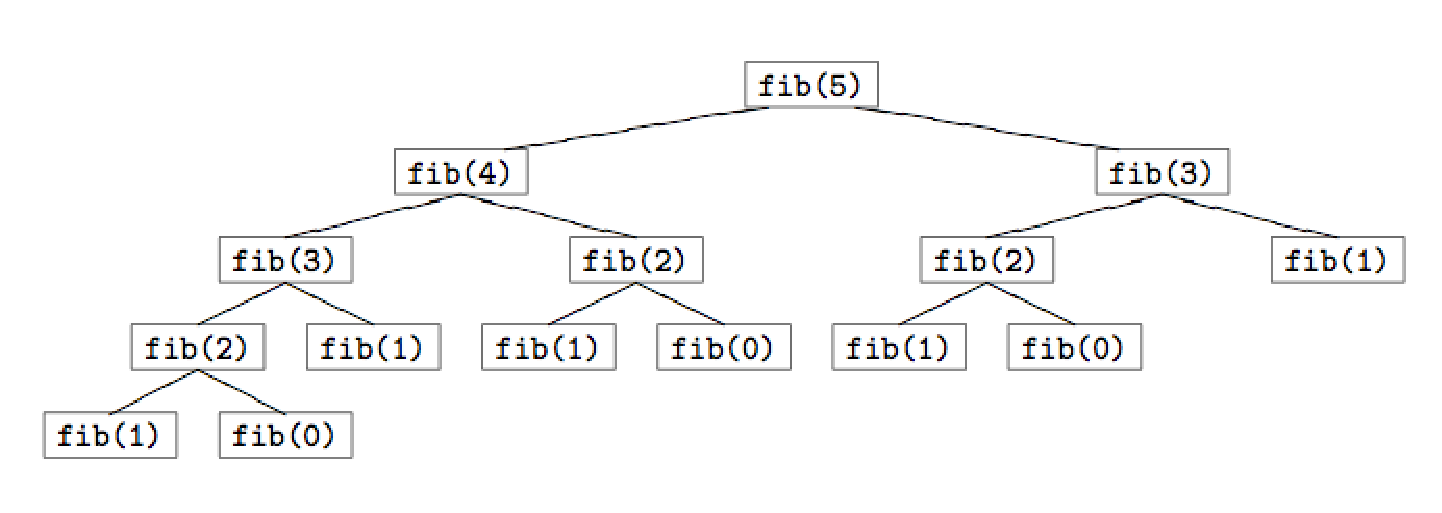
\epsfig{file=Abbildungen/fibonacci.eps, scale=0.6}} 
  \caption{Rekursions-Baum für die Berechnung von $\textsl{fibonacci}(5)$.}
  \label{fig:fibonacci.eps}
\end{figure}


Wir können eine effizientere Berechnung der Fibonacci-Zahlen implementieren, indem wir
uns die berechneten Werte merken.  Dazu können wir eine Liste benutzen.
 Dies führt zu dem in Abbildung \ref{fig:fibonacci-dynamic}
auf Seite \pageref{fig:fibonacci-dynamic} angegebenen Programm.  
 Da die Fibonacci-Zahlen $f_n$ mit $n=0$ beginnen, die Elemente einer Liste aber mit
1 beginnend indiziert werden, wird der Wert
\\[0.2cm]
\hspace*{1.3cm}
$\textsl{fibonacci(i)}$ \quad in der Liste $l$ an der Stelle \quad $l(i+1)$
\\[0.2cm]
gespeichert. 

\begin{figure}[!h]
  \centering
\begin{Verbatim}[ frame         = lines, 
                  framesep      = 0.3cm, 
                  labelposition = bottomline,
                  numbers       = left,
                  numbersep     = -0.2cm,
                  xleftmargin   = 0.8cm,
                  xrightmargin  = 0.8cm
                ]
    fibonacci := procedure(n) {
        l := [1, 1] + [2 .. n];
        for (k in [ 2 .. n ]) {
            l(k+1) := l(k) + l(k-1);
        }
        return l(n+1);
    };
    
    for (n in [0 .. 10000]) {
        print("fibonacci($n$) = $fibonacci(n)$");
    }
\end{Verbatim}
\vspace*{-0.3cm}
  \caption{Berechnung der Fibonacci-Zahlen mit Speicherung der Zwischenwerte.}
  \label{fig:fibonacci-dynamic}
\end{figure} 


\section{Lineare Rekurrenz-Gleichung \label{sec:lineare-RG}}
Wir waren bei der Analyse der Komplexität des ersten Programms zur Berechnung der
Fibonacci-Zahlen auf die Gleichung \\[0.2cm]
\hspace*{1.3cm} $a_{i+2} = a_{i+1} + {a_i} + 1$ \quad für alle $i \in \mathbb{N}$ \\[0.2cm]
gestoßen. Gleichungen dieser Form treten bei der Analyse der Komplexität rekursiver
Programme häufig auf. Wir wollen uns daher in diesem Abschnitt näher mit solchen
Gleichungen beschäftigen.

\begin{Definition}[Lineare homogene Rekurrenz-Gleichung] \hspace*{\fill} \\
{\em 
  Die \emph{lineare homogene Rekurrenz-Gleichung der Ordnung $k$ mit konstanten Koeffizienten} hat die Form
  \begin{equation}
    \label{eq:lhrg}
  a_{n+k} = c_{k-1} \cdot a_{n+k-1} + c_{k-2} \cdot a_{n+k-2} + \cdots + c_1 \cdot a_{n+1} + c_0 \cdot a_{n}
     \quad \mbox{für alle $n \in \mathbb{N}$}. 
  \end{equation}
     In Summen-Schreibweise kann diese Gleichung kompakter als 
     \\[0.2cm]
     \hspace*{1.3cm}
     $a_{n+k} = \sum\limits_{i=0}^{k-1} c_i \cdot a_{n+i}$ \quad für alle $n \in \mathbb{N}$
     \\[0.2cm]
     geschreiben werden.
     Zusätzlich werden \emph{Anfangs-Bedingungen}  
      \\[0.2cm]
      \hspace*{1.3cm}      
      $a_0 = d_0, \cdots, a_{k-1} = d_{k-1}$ 
      \\[0.2cm]
      für die Folge $\folge{a_n}$ vorgegeben.    
    \hspace*{\fill} $\Box$
}
\end{Definition}
Durch eine lineare homogene Rekurrenz-Gleichung wird die Folge $(a_n)_{n\in\mathbb{N}}$
eindeutig bestimmt: Die Werte $a_n$ für $n < k$ sind durch die Anfangs-Bedingungen gegeben und
alle weiteren Werte können dann durch die Rekurrenz-Gleichung (\ref{eq:lhrg}) bestimmt werden.
Noch  etwas zur Nomenklatur:
\begin{enumerate}
\item Die Rekurrenz-Gleichung (\ref{eq:lhrg}) heißt \emph{linear}, weil die Glieder der Folge $(a_n)_n$ nur
      linear in der Gleichung (\ref{eq:lhrg}) auftreten.  Ein Beispiel für eine
      Rekurrenz-Gleichung, die nicht linear ist, wäre \\[0.2cm]
      \hspace*{1.3cm} $a_{n+1} = a_n^2$ \quad für alle $n \in \mathbb{N}$. \\[0.2cm]
      Nicht-lineare Rekurrenz-Gleichungen sind nur in Spezialfällen geschlossen lösbar.
\item Die Rekurrenz-Gleichung (\ref{eq:lhrg}) heißt \emph{homogen}, weil auf der rechten Seite
      dieser Gleichung kein konstantes Glied mehr auftritt.  Ein Beispiel für eine
      Gleichung, die nicht homogen ist (wir sprechen auch von \emph{inhomogenen}
      Rekurrenz-Gleichungen), wäre \\[0.2cm]
      \hspace*{1.3cm} $a_{n+2} = a_{n+1} + a_n + 1$ \quad für alle $n \in \mathbb{N}$. \\[0.2cm]
      Mit inhomogenen Rekurrenz-Gleichungen werden wir uns später noch beschäftigen.
\item Die Rekurrenz-Gleichung (\ref{eq:lhrg}) hat \emph{konstante Koeffizienten}, weil die
      Werte $c_i$ Konstanten sind, die nicht von dem Index $n$ abhängen.  Ein Beispiel für
      eine Rekurrenz-Gleichung, die keine konstanten Koeffizienten hat, ist \\[0.2cm]
      \hspace*{1.3cm} $a_{n+1} = n\cdot a_n$ \quad für alle $n \in \mathbb{N}$. \\[0.2cm]
      Solche Rekurrenz-Gleichungen können in vielen Fällen auf Rekurrenz-Gleichungen mit
      konstanten Koeffizienten zurück geführt werden.  Wir werden das später noch im
      Detail besprechen.
\end{enumerate}
Wie lösen wir eine lineare homogene Rekurrenz-Gleichung?  Wir versuchen zunächst den Ansatz\\[0.2cm]
\hspace*{1.3cm}  $a_n = \lambda^n$ \quad für alle $n \in \mathbb{N}$. \\[0.2cm]
Einsetzen dieses Ansatzes in (\ref{eq:lhrg}) führt auf die Gleichung \\[0.2cm]
\hspace*{1.3cm}
$\lambda^{n+k} = \sum\limits_{i=0}^{k-1} c_i \cdot \lambda^{n+i}$
\\[0.2cm]
Dividieren wir diese Gleichung durch $\lambda^n$, so haben wir: \\[0.2cm]
\hspace*{1.3cm} $\lambda^{k} = \sum\limits_{i=0}^{k-1} c_i \cdot \lambda^{i}$  
\\[0.2cm]
Das Polynom \\[0.2cm]
\hspace*{1.3cm} 
$\chi(x) = x^{k} - \sum\limits_{i=0}^{k-1} c_i \cdot x^{i}$  
\\[0.2cm]
 heißt \emph{charakteristisches Polynom} der Rekurrenz-Gleichung (\ref{eq:lhrg}).
Wir betrachten zunächst den Fall, dass das charakteristische  Polynom  $k$  verschiedene
Nullstellen hat.  In diesem Fall sagen, dass die Rekurrenz-Gleichung (\ref{eq:lhrg}) 
\emph{nicht entartet} ist.
Bezeichnen wir diese Nullstellen mit \\[0.2cm]
\hspace*{1.3cm}  $\lambda_1$, $\lambda_2$, $\cdots$, $\lambda_k$, \\[0.2cm]
so  gilt für alle $j = 1,\cdots, k$ \\[0.2cm]
\hspace*{1.3cm} 
$\lambda_j^{n+k} = \sum\limits_{i=0}^{k-1} c_i \cdot \lambda_j^{n+i}$.
\\[0.2cm]
Damit ist die Folge  
\[\bigl(\lambda_j^n)_{n\in\mathbb{N}}\]
für alle $j=1,\cdots,k$ eine Lösung der Rekurrenz-Gleichung (\ref{eq:lhrg}).
Außerdem ist auch jede Linear-Kombination dieser Lösungen eine Lösung von (\ref{eq:lhrg}):
Definieren wir die Folge $a_n$ durch \\[0.2cm]
\hspace*{1.3cm} 
$a_n = \alpha_1 \cdot \lambda_1^n + \cdots + \alpha_k \cdot \lambda_k^n$ \quad für alle $n
\in \mathbb{N}$ 
\\[0.2cm]
mit beliebigen Koeffizienten $\alpha_i \in \mathbb{R}$, so erfüllt auch die Folge
$(a_n)_n$ die Gleichung (\ref{eq:lhrg}).  Die oben definierte Folge $(a_n)_n$ bezeichnen wir als
die  \emph{allgemeine Lösung} der Rekurrenz-Gleichung (\ref{eq:lhrg}). 
Die Koeffizienten $\alpha_i$ müssen wir für $i=1,\;\cdots,\;k$ so wählen, dass die
Anfangs-Bedingungen 
\\[0.2cm]
\hspace*{1.3cm}
$a_0 = d_0$, $\cdots$, $a_{k-1} = d_{k-1}$
\\[0.2cm]
erfüllt sind.  Das liefert ein lineares Gleichungs-System für die Koeffizienten $\alpha_1$, $\cdots$, $\alpha_k$:
\[
\begin{array}{lcl}
  d_0     & = & \lambda_1^0 \cdot \alpha_1 + \cdots +   \lambda_k^0 \cdot \alpha_k \\[0.2cm]
  d_1     & = & \lambda_1^1 \cdot \alpha_1 + \cdots +   \lambda_k^1 \cdot \alpha_k \\[0.2cm]
  \vdots  &   & \vdots                                                   \\[0.2cm]
  d_{k-1} & = & \lambda_1^{k-1} \cdot \alpha_1 + \cdots +   \lambda_{k}^{k-1} \cdot \alpha_k \\[0.2cm]
\end{array}
\]
Hier sind die Werte $\lambda_i$  die Nullstellen des charakteristischen Polynoms.  
Die Matrix $V$, die diesem Gleichungs-System
zugeordnet ist, lautet: 
\[
V = \left(
\begin{array}{lcl}
  \lambda_1^0  & \cdots &   \lambda_k^0 \\[0.2cm]
  \lambda_1^1  & \cdots &   \lambda_k^1 \\[0.2cm]
  \vdots         &         & \vdots \\[0.2cm]
  \lambda_1^{k-1} & \cdots &   \lambda_{k}^{k-1} \\[0.2cm]
\end{array}\right)
\]
Diese Matrix ist in der Mathematik als \emph{Vandermonde}'sche Matrix bekannt.  
Es lässt sich zeigen, dass ein Gleichungs-System, das mit dieser Matrix gebildet wird,
genau dann eindeutig lösbar ist, wenn die Nullstellen $\lambda_i$ für $i=1,\cdots,k$
paarweise verschieden sind.
\vspace*{0.2cm}

\noindent
\textbf{Beispiel}:  Wie demonstrieren das Verfahren an einem Beispiel: Wie betrachten die
Rekurrenz-Gleichung \\[0.2cm]
\hspace*{1.3cm} $F_{n+2} = F_{n+1} + F_{n}$ \quad für alle $n \in \mathbb{N}$  \\[0.2cm]
mit den Anfangs-Bedingungen $F_0 = 0$ und $F_1 = 1$.  Die Lösung dieser
Rekurrenz-Gleichung sind übrigens gerade die Fibonacci-Zahlen.
Das \emph{charakteristische Polynom} dieser Rekurrenz-Gleichung lautet: \\[0.2cm]
\hspace*{1.3cm} $\chi(x) = x^2 - x - 1$.  \\[0.2cm]
Das führt auf die quadratische Gleichung \\[0.2cm]
\hspace*{1.3cm} $x^2 -x - 1 = 0$ \\[0.2cm]
Wir haben eben schon gesehen, dass diese quadratische Gleichung die Lösung \\[0.2cm]
\hspace*{1.3cm}
 $ x_{1/2} = \frac{1}{2} \cdot (1 \pm \sqrt{5})$ 
\\[0.2cm]
hat.  Wir definieren \\[0.2cm]
\hspace*{1.3cm} 
$\lambda_1 = \frac{1}{2} \cdot (1 + \sqrt{5})$ \quad und  \quad 
$\lambda_2 = \frac{1}{2} \cdot (1 - \sqrt{5})$. \\[0.2cm]
Damit lautet die \emph{allgemeine Lösung} der betrachteten Rekurrenz-Gleichung \\[0.2cm]
\hspace*{1.3cm}  $F_n = \alpha_1 \cdot \lambda_1^n  + \alpha_2 \cdot \lambda_2^n$ \quad für alle $n \in \mathbb{N}$. \\[0.2cm]
Setzen wir hier die Anfangs-Bedingungen ein, so erhalten wir
\[
\begin{array}{lcl}
    0 & = & \lambda_1^0 \cdot \alpha_1 + \lambda_2^0   \cdot \alpha_2 \\[0.2cm]
    1 & = & \lambda_1^1 \cdot \alpha_1 + \lambda_2^{1} \cdot \alpha_2 
\end{array}
\]
Dies ist ein lineares Gleichungs-System in den Unbekannten $\alpha_1$ und
$\alpha_2$. Vereinfachung führt auf 
\[
\begin{array}{lcl}
    0 & = & \alpha_1 + \alpha_2 \\[0.2cm]
    1 & = & \lambda_1 \cdot \alpha_1 + \lambda_2 \cdot \alpha_2 
\end{array}
\]
Die erste dieser beiden Gleichungen lösen wir nach $\alpha_2$ auf und finden  $\alpha_2 = - \alpha_1$.
Diesen Wert setzen wir in der zweiten Gleichung ein.  Das führt auf
\[
\begin{array}{lrcl}
                 & 1 & = & \lambda_1 \cdot \alpha_1 - \lambda_2 \cdot \alpha_1 \\[0.2cm]
 \Leftrightarrow & 1 & = & (\lambda_1 - \lambda_2) \cdot \alpha_1              \\[0.2cm]
 \Leftrightarrow & \bruch{1}{\lambda_1 - \lambda_2} & = & \alpha_1 
\end{array}
\]
Setzen wir diesen Wert in die Gleichung $\alpha_2 = - \alpha_1$ ein, so erhalten wir \\[0.2cm]
\hspace*{1.3cm} 
  $\alpha_2 = \bruch{- 1}{\lambda_1 - \lambda_2}$.
\\[0.2cm]
Setzen wir die  Werte für $\lambda_1$ und $\lambda_2$ ein, so finden wir:  \\[0.2cm]
\hspace*{1.3cm} 
$\alpha_1 = \bruch{1}{\sqrt{5}}$ \quad und \quad $\alpha_2 = - \bruch{1}{\sqrt{5}}$.
\\[0.2cm]
Die Lösung der Rekurrenz-Gleichung \\[0.2cm]
\hspace*{1.3cm} $F_{n+2} = F_{n+1} + F_{n}$ \quad für alle $n \in \mathbb{N}$ \\[0.2cm]
mit den Anfangs-Bedingungen $F_0 = 1$ und $F_1 = 1$   lautet also 
\\[0.2cm]
\hspace*{1.3cm} 
$F_n = \bruch{1}{\sqrt{5}}\cdot \left( \lambda_1^{n} - \lambda_2^{n} \right)$ 
\quad für alle $n \in \mathbb{N}$.  
\\[0.2cm]
Damit haben wir eine geschlossene Formel zur Berechnung der Fibonacci-Zahlen
gefunden.  Diese Formel zeigt uns, dass die Fibonacci-Zahlen selbst exponentiell anwachsen.
Wir werden diese Formel später bei der Analyse des Laufzeitverhaltens des
Euklidischen-Algorithmus benötigen. 

\vspace*{0.2cm}
\noindent
\textbf{Aufgabe}:  Lösen Sie die Rekurrenz-Gleichung 
$a_{n+2} = \bruch{3}{2} \cdot a_{n+1} - \bruch{1}{2}\cdot a_n$ mit
den Anfangs-Bedingungen $a_0 = 3$ und $a_1 = \bruch{5}{2}$.

%\noindent
%\textbf{Lösung}: $a_n = 2 + \left(\frac{1}{2}\right)^n$.

\subsection{Entartete Rekurrenz-Gleichungen}
Wir hatten oben zunächst den Fall betrachtet, dass das charakteristische Polynom der
Rekurrenz-Gleichung (\ref{eq:lhrg}) insgesamt $k$ verschiedene Nullstellen hat.   Dies muss
keineswegs immer der Fall sein.  Wir betrachten die Rekurrenz-Gleichung 
\begin{equation}
  \label{eq:erg}
  a_{n+2} = 4 \cdot a_{n+1} - 4 \cdot a_n \quad \mbox{für alle $n \in \mathbb{N}$} 
\end{equation}
 mit den Anfangs-Bedingungen $a_0 = 1$, $a_1 = 4$.  Das charakteristische Polynom lautet \\[0.2cm]
\hspace*{1.3cm} $\chi(x) = x^2 - 4 \cdot x + 4 = (x - 2)^2$ \\[0.2cm]
und hat offensichtlich nur eine Nullstelle bei $x = 2$.   Eine Lösung der
Rekurrenz-Gleichung (\ref{eq:erg}) lautet daher \\[0.2cm]
\hspace*{1.3cm} $a_n = 2^n$ \quad für alle $n \in \mathbb{N}$. \\[0.2cm]
Eine weitere Lösung ist \\[0.2cm]
\hspace*{1.3cm} $a_n = n \cdot 2^n$ \quad für alle $n \in \mathbb{N}$.  \\[0.2cm]
Wir verifizieren dies durch Einsetzen: 
\[
\begin{array}{llcll}
 & (n+2) \cdot 2^{n+2} & = & 4 \cdot (n+1) \cdot 2^{n+1} - 4 \cdot n \cdot 2^n & \mid\; \div 2^n \\
\Leftrightarrow & 
   (n+2) \cdot 2^{2} & = & 4 \cdot (n+1) \cdot 2^{1} - 4 \cdot n  &  \mid\; \div 4 \\
\Leftrightarrow & n + 2 & = & (n + 1) \cdot 2 -  n  &  \\
\Leftrightarrow & n + 2 & = & 2 \cdot n + 2 -  n   \\
\Leftrightarrow & n + 2 & = & n + 2    \\
\end{array}
\]
Die allgemeine Lösung der Rekurrenz-Gleichung finden wir durch Linear-Kombination der
beiden Lösungen: \\[0.2cm]
\hspace*{1.3cm} $a_n = \alpha \cdot 2^n + \beta \cdot n \cdot 2^n$ \quad für alle $n \in \mathbb{N}$. \\[0.2cm]
Setzen wir hier die Anfangs-Bedingungen $a_0 = 1$ und $a_2 = 4$ ein, so erhalten wir:
\[
\left\{
\begin{array}{lcl}
  1 & = & \alpha \cdot 2^0 + \beta \cdot 0 \cdot 2^0 \\
  4 & = & \alpha \cdot 2^1 + \beta \cdot 1 \cdot 2^1 \\
\end{array}
\right\} \quad\Leftrightarrow\quad \left\{
\begin{array}{lcl}
  1 & = & \alpha \\
  4 & = & \alpha \cdot 2 + \beta \cdot 2 \\
\end{array}
\right\}\]
Die Lösung lautet offenbar $\alpha = 1$ und $\beta = 1$.  Damit lautet die Lösung der
Rekurrenz-Gleichung (\ref{eq:erg}) mit den Anfangs-Bedingungen $a_0 = 1$ und $a_2 = 4$ \\[0.2cm]
\hspace*{1.3cm} $a_n = 2^n + n \cdot 2^n = (n+1) \cdot 2^n$ \quad für alle $n \in \mathbb{N}$.  \\[0.2cm]
Im allgemeinen nennen wir die Rekurrenz-Gleichung \\[0.2cm]
\hspace*{1.3cm} $a_{n+k} = \sum\limits_{i=0}^{k-1} c_{i} \cdot a_{n+i}$ \\[0.2cm]
\emph{entartet}, wenn das charakteristische Polynom \\[0.2cm]
\hspace*{1.3cm} $\chi(x) = x^k - \sum\limits_{i=0}^{k-1} c_{i} \cdot x^{i}$  \\[0.2cm]
weniger als $k$ verschiedene Nullstellen hat.  Dann lässt sich folgendes
zeigen:  Hat das charakteristische Polynom $\chi(x)$ eine $r$-fache Nullstelle
$\lambda$, gilt also \\[0.2cm]
\hspace*{1.3cm} $\chi(x) = (x - \lambda)^r \cdot \phi(x)$ \\[0.2cm]
mit einem geeigneten Polynom $\phi(x)$, so sind die Folgen
\begin{enumerate}
\item $(\lambda^n)_{n\in\mathbb{N}}$
\item $(n\cdot\lambda^n)_{n\in\mathbb{N}}$
\item $(n^2\cdot\lambda^n)_{n\in\mathbb{N}}$
\item $\vdots$
\item $(n^{r-1}\cdot\lambda^n)_{n\in\mathbb{N}}$
\end{enumerate}
Lösungen der Rekurrenz-Gleichung (\ref{eq:erg}).  Durch eine geeignete Linear-Kombination dieser
Lösungen zusammen mit den Lösungen, die sich aus den anderen Nullstellen des Polynoms $\phi$
ergeben, lässt sich dann immer eine Lösung finden, die auch den Anfangs-Bedingungen genügt.
\vspace*{0.3cm}

\noindent
\textbf{Aufgabe}: Lösen Sie die Rekurrenz-Gleichung \\[0.2cm]
\hspace*{1.3cm} $a_{n+3} = a_{n+2} + a_{n+1} - a_n$ \\[0.2cm]
für die Anfangs-Bedingungen $a_0 = 0$, $a_1 = 3$, $a_2 = 2$.

%\noindent
%\textbf{Lösung}: allg. $a_n = \alpha + n \cdot \beta + \gamma \cdot (-1)^n$. 
%Anfangs-Bedingungen: $a_n = 1 + n - (-1)^n$.
\pagebreak

\subsection{Inhomogene Rekurrenz-Gleichungen}    
\begin{Definition}[Lineare inhomogene Rekurrenz-Gleichung] \lb
{\em Die \emph{lineare \underline{inhomo}g\underline{ene} Rekur\-renz-Gleichung der Ordnung
$k$ mit konstanten Koeffizienten und konstanter Inhomogenität} hat die Form 
\begin{equation}
  \label{eq:lihrg}
     a_{n+k} = \sum\limits_{i=0}^{k-1} c_{i} \cdot a_{n+i} + c_{-1}  
\end{equation}
     mit den Anfangs-Bedingungen $a_0 = d_0$, $\cdots$, $a_{k-1} = d_{k-1}$. 
     Dabei gilt für die Koeffizienten \\[0.2cm]
     \hspace*{1.3cm} $c_i \in \mathbb{R}$ \quad für alle $i = -1, 0,\cdots, k-1$. \\[0.2cm]
     Für die  \emph{Anfangs-Bedingungen} $d_0, \cdots, d_{k-1}$ gilt ebenfalls \\[0.2cm]
     \hspace*{1.3cm} $d_i \in \mathbb{R}$ \quad für alle $i = 0,\cdots, k-1$. \\[0.2cm]
     Die Konstante $c_{-1}$ bezeichnen wir als die \emph{Inhomogenität}. 
     \hspace*{\fill} $\Box$
}
\end{Definition}

Wie lässt sich die inhomogene Rekurrenz-Gleichung (\ref{eq:lihrg}) lösen? Wir zeigen
zunächst, wie sich eine \emph{spezielle Lösung} der Rekurrenz-Gleichung (\ref{eq:lihrg})
finden lässt.  Dazu betrachten wir das charakteristische Polynom \\[0.2cm]
\hspace*{1.3cm} 
$\chi(x) = x^k - \sum\limits_{i=0}^{k-1} c_{i} \cdot x^i$
\\[0.2cm]
und definieren die \emph{Spur} $\mathtt{sp}(\chi)$ wie folgt: \\[0.2cm]
\hspace*{1.3cm} 
$\mathtt{sp}(\chi) := \chi(1) = 1 - \sum\limits_{i=0}^{k-1} c_{i}$. \\[0.2cm]
Es können zwei Fälle auftreten, $\mathtt{sp}(\chi) \not= 0$ und
$\mathtt{sp}(\chi) = 0$.
Wir betrachten die beiden Fälle getrennt.
\begin{enumerate}
\item $\mathtt{sp}(\chi) \not= 0$.

      Dann erhalten wir eine spezielle Lösung von (\ref{eq:lihrg}) durch den Ansatz \\[0.2cm]
      \hspace*{1.3cm} $a_n = \delta$ \quad für alle $n \in \mathbb{N}$. \\[0.2cm]
      Den Wert von $\delta$ bestimmen wir durch Einsetzen, es muss für alle $n\in \mathbb{N}$ gelten: \\[0.2cm]
      \hspace*{1.3cm} 
      $\delta = \sum\limits_{i=0}^{k-1} c_{i} \cdot \delta + c_{-1}$.
      \\[0.2cm]
      Daraus ergibt sich \\[0.2cm]
      \hspace*{1.3cm} 
      $\delta \cdot \left(1 - \sum\limits_{i=0}^{k-1} c_{i} \right) =  c_{-1}$. \\[0.2cm]
      Das ist aber nichts anderes als \\[0.2cm]
      \hspace*{1.3cm} $\delta \cdot \mathtt{sp}(\chi) = c_{-1}$ \\[0.2cm]
      und damit lautet eine spezielle Lösung von (\ref{eq:lihrg}) \\[0.2cm]
      \hspace*{1.3cm} $a_n = \delta = \bruch{c_{-1}}{\mathtt{sp}(\chi)}$.
      \\[0.2cm]
      Jetzt sehen wir auch, warum die Voraussetzung $\mathtt{sp}(\chi) \not= 0$
      wichtig ist, denn anderfalls wäre der Quotient
      $\bruch{c_{-1}}{\mathtt{sp}(\chi)}$ undefiniert.
\item $\mathtt{sp}(\chi) = 0$.

      In diesem Fall versuchen wir, eine spezielle Lösung von (\ref{eq:lihrg}) durch den
      Ansatz \\[0.2cm]
      \hspace*{1.3cm} $a_n = \varepsilon \cdot n $ \\[0.2cm]
      zu finden.  Den Wert $\varepsilon$ erhalten wir durch Einsetzen, es muss für 
      alle $n\in\mathbb{N}$ gelten: \\[0.2cm]
      \hspace*{1.3cm} 
      $\varepsilon \cdot (n + k) = \sum\limits_{i=0}^{k-1} c_{i} \cdot \varepsilon \cdot (n + i) + c_{-1}$  
      \\[0.2cm]
      Dies formen wir wie folgt um:
      \[
        \varepsilon \cdot n + \varepsilon \cdot k = 
        \varepsilon \cdot n \cdot \sum\limits_{i=0}^{k-1} c_{i} +
        \varepsilon \cdot \sum\limits_{i=0}^{k-1} i \cdot c_{i} + c_{-1} 
      \]
      Aus  $\mathtt{sp}(\chi) = 0$ folgt $1  =  \sum\limits_{i=0}^{k-1} c_i$
      und damit gilt \\[0.2cm]
      \hspace*{1.3cm} 
      $\varepsilon \cdot n = \varepsilon \cdot n \cdot \sum\limits_{i=0}^{k-1} c_{i}$.
      \\[0.2cm]
      Daher vereinfacht sich die obige Gleichung zu 
      \[
      \begin{array}{ll}
      & \varepsilon \cdot k = \varepsilon \cdot \sum\limits_{i=0}^{k-1} i \cdot c_{i} + c_{-1} \\[0.4cm]
      \Leftrightarrow\quad 
      & \varepsilon \cdot \left(k - \sum\limits_{i=0}^{k-1} i \cdot c_{i}\right) = c_{-1} 
      \\[0.5cm]
      \Leftrightarrow\quad 
      & \varepsilon = \frac{\displaystyle c_{-1}}{\displaystyle \; k - \sum\limits_{i=0}^{k-1} i \cdot c_{i}\;} 
      \end{array}
      \]
      Wenn wir genau hin schauen, dann sehen wir, dass der Wert im Nenner nicht anderes ist
      als der Wert der Ableitung des charakteristischen Polynoms an der Stelle 1, denn es gilt: \\[0.2cm]
      \hspace*{1.3cm} 
      $\chi'(x) =\frac{d\;}{dx}\chi(x) = k \cdot x^{k-1} - \sum\limits_{i=1}^{k-1} c_{i}\cdot i \cdot x^{i-1}$
      \\[0.2cm]
      Setzen wir hier für $x$ den Wert $1$ ein, so finden wir \\[0.2cm]
      \hspace*{1.3cm} 
      $\chi'(1) = k - \sum\limits_{i=1}^{k-1} c_{i}\cdot i =  k - \sum\limits_{i=0}^{k-1} c_{i}\cdot i$. 
      \\[0.2cm]
      Insgesamt haben wir damit also die folgende spezielle Lösung $(a_n)_{n\in\mathbb{N}}$
      der Gleichung (\ref{eq:lihrg}) gefunden: \\[0.2cm]
      \hspace*{1.3cm} $a_n = \bruch{c_{-1}}{\;\chi'(1)\;}\cdot n$.

      Wir haben oben zur Vereinfachung angenommen, dass dieser Wert von 0 verschieden ist,
      dass also das charakteristische Polynom $\chi(x)$ an der Stelle $x=1$ keine mehrfache
      Nullstelle hat, denn nur dann ist $\varepsilon$ durch die
      obige Gleichung wohldefiniert und wir haben eine spezielle Lösung der
      Rekurrenz-Gleichung (\ref{eq:lihrg}) gefunden.  Andernfalls können wir die Reihe nach die
      Ansätze $a_n = \varepsilon \cdot n^2$, $a_n = \varepsilon \cdot n^3$ , $\cdots$
      versuchen, denn es kann folgendes gezeigt werden: 
      Hat das charakteristische Polynom $\chi(x)$ am Punkt $x = 1$ eine Nullstelle vom Rang $r$,
      so führt der Ansatz $a_n = \varepsilon \cdot n^r$ zu einer speziellen Lösung von (\ref{eq:lihrg}).
\end{enumerate}
Diese spezielle Lösung genügt i.~a.~noch nicht den
Anfangs-Bedingungen. Eine Lösung, die auch den Anfangs-Bedingungen genügt, erhalten wir,
wenn wir zu der speziellen Lösung die allgemeine Lösung der zugehörigen homogenen linearen
Rekurrenz-Gleichung \\[0.2cm]
\hspace*{1.3cm} 
     $a_{n+k} = c_{k-1} \cdot a_{n+k-1} + c_{k-2} \cdot a_{n+k-2} + \cdots + c_1 \cdot a_{n+1} + c_0 \cdot a_{n}$ 
\\[0.2cm]
addieren und die Koeffizienten der allgemeinen Lösung so wählen, dass die
Anfangs-Bedingungen erfüllt sind.  Wir betrachten  ein Beispiel:
 Die zu lösende Rekurrenz-Gleichung lautet \\[0.2cm]
\hspace*{1.3cm} $a_{n+2} = 3 \cdot a_{n+1} - 2 \cdot a_n -1$ \quad für alle $n \in \mathbb{N}$. \\[0.2cm]
Die Anfangs-Bedingungen sind $a_0 = 1$ und $a_1 = 3$.  Wir berechnen zunächst eine
spezielle Lösung.  Das charakteristische Polynom ist \\[0.2cm]
\hspace*{1.3cm} $\chi(x) = x^2 -3 \cdot x +2 = (x - 1) \cdot (x - 2)$. \\[0.2cm]
Es gilt $\mathtt{sp}(\chi) = \chi(1) = 0$.  Wir versuchen für die spezielle Lösung
den Ansatz \\[0.2cm]
\hspace*{1.3cm} $a_n = \varepsilon \cdot n$. \\[0.2cm]
Einsetzen in die Rekurrenz-Gleichung liefert \\[0.2cm]
\hspace*{1.3cm}  $\varepsilon \cdot (n+2) = 3 \cdot \varepsilon \cdot(n+1) - 2 \cdot \varepsilon \cdot n -1$ \quad für alle $n \in \mathbb{N}$. \\[0.2cm]
Das ist äquivalent zu \\[0.2cm]
\hspace*{1.3cm} $\varepsilon \cdot (2 - 3) = - 1$ \\[0.2cm]
und daraus folgt sofort $\varepsilon = 1$.  Damit lautet eine spezielle Lösung \\[0.2cm]
\hspace*{1.3cm} $a_n = n$ \quad für alle $n \in \mathbb{N}$. \\[0.2cm]
Da die Nullstellen des charakteristischen Polynoms $\chi(x)$ bei 1 und 2 liegen, finden
wir für die allgemeine Lösung 
\\[0.2cm]
\hspace*{1.3cm} $a_n = \alpha \cdot 1^n + \beta \cdot 2^n + n$ \quad für alle $n \in \mathbb{N}$. \\[0.2cm]
Setzen wir hier für $n$ die Werte $0$ und $1$ und für $a_n$ die beiden Anfangs-Bedingungen
ein, so erhalten wir das Gleichungs-System \\[0.2cm]
\[ \left\{
\begin{array}{lcl}
1 &=& \alpha \cdot 1^0 + \beta \cdot 2^0 + 0 \\
3 &=& \alpha \cdot 1^1 + \beta \cdot 2^1 + 1
\end{array} \right\} \Leftrightarrow \left\{
\begin{array}{lcl}
1 &=& \alpha + \beta  \\
3 &=& \alpha + 2 \cdot \beta + 1
\end{array} \right\}\]
Sie können leicht nachrechnen, dass dieses Gleichungs-System die Lösung $\alpha = 0$ und
$\beta = 1$ hat.  Damit lautet die Lösung der Rekurrenz-Gleichung \\[0.2cm]
\hspace*{1.3cm} $a_n = 2^n + n$ \quad für alle $n \in \mathbb{N}$.
\vspace*{0.3cm}

\noindent
\textbf{Aufgabe}: Lösen Sie die inhomogene Rekurrenz-Gleichung \\[0.2cm]
\hspace*{1.3cm} $a_{n+2} = 2 \cdot a_n - a_{n+1} + 3$ \\[0.2cm]
für die Anfangs-Bedingungen $a_0 = 2$ und $a_1 = 1$.
% charakteristisches Polynom: $\chi(x) = x^2 + x - 2 = (x - 1) * (x + 2)
% sp(\chi) = 0, \chi'(x) = 2*x + 1, \chi'(1) = 3
% Lsg: a_n = \varepsilon * n mit \varepsilon = 1
% Lsg: a_n = 4/3 + 2/3*(-2)^n + n

\subsection{Lineare inhomogene Rekurrenz-Gleichungen mit veränderlichen Inhomogenitäten}
Gelegentlich tauchen in der Praxis Rekurrenz-Gleichungen auf, in denen die Inhomogenität
keine Konstante ist, sondern von $n$ abhängt.  In solchen Fällen führt die
Technik des \emph{diskreten Differenzieren} oft zum Erfolg.  Wir stellen die Technik an
einem Beispiel vor und betrachten die Rekurrenz-Gleichung 
\begin{equation}
  \label{eq:dd}
a_{n+1} = 2 \cdot a_n + n \quad \mbox{für alle $n \in \mathbb{N}$}  
\end{equation}
und der Anfangs-Bedingungen $a_0 = 0$.  Das Verfahren zur Lösung solcher
Rekurrenz-Gleichung besteht aus vier Schritten:
\begin{enumerate}
\item Substitutions-Schritt: Im \emph{Substitutions-Schritt} setzen wir in der
      ursprünglichen Rekurrenz-Gleichung (\ref{eq:dd}) für $n$ den Wert $n + 1$ ein und
      erhalten 
      \begin{equation}
        \label{eq:dd2}
        a_{n+2} = 2 \cdot a_{n+1} + n + 1 \quad \mbox{für alle $n \in \mathbb{N}$}
      \end{equation}
\item Subtraktions-Schritt: Im \emph{Subtraktions-Schritt} ziehen wir von der im
      Substitutions-Schritt erhaltenen Rekurrenz-Gleichung (\ref{eq:dd2}) die ursprüngliche
      gegebene Rekurrenz-Gleichung (\ref{eq:dd}) ab.  In unserem Fall erhalten wir \\[0.2cm]
      \hspace*{1.3cm} 
      $a_{n+2} - a_{n+1} = 2 \cdot a_{n+1} + n + 1 - \left( 2 \cdot a_n + n \right)$ 
      \quad für alle $n \in \mathbb{N}$.       \\[0.2cm]
      Vereinfachung dieser Gleichung liefert 
      \begin{equation}
        \label{eq:dd3}
        a_{n+2} = 3 \cdot a_{n+1} - 2 \cdot a_n + 1 \quad \mbox{für alle $n \in \mathbb{N}$}.
      \end{equation}
      Die beiden Schritte 1.~und 2.~bezeichnen wir zusammen als 
      \emph{diskretes Differenzieren} der Rekurrenz-Gleichung.
\item Berechnung zusätzlicher Anfangs-Bedingungen: Die Rekurrenz-Gleichung (\ref{eq:dd3})
      ist eine inhomogene Rekurrenz-Gleichung der Ordnung 2 mit nun aber konstanter
      Inhomogenität.  Wir haben bereits gesehen, 
      wie eine solche Rekurrenz-Gleichung zu lösen ist, wir benötigen aber eine
      zusätzliche Anfangs-Bedingung für $n=1$.  Diese erhalten wir, indem wir in der
      ursprünglichen Rekurrenz-Gleichung (\ref{eq:dd}) für $n$ den Wert 0 einsetzen: \\[0.2cm]
      \hspace*{1.3cm} $a_1 = 2 \cdot a_0 + 0 = 0$.
\item Lösen der inhomogenen Rekurrenz-Gleichung mit konstanter Inhomogenität:
      Das charakteristische Polynom der Rekurrenz-Gleichung (\ref{eq:dd3}) lautet: \\[0.2cm]
      \hspace*{1.3cm} $\chi(x) = x^2 - 3 \cdot x + 2 = (x - 2) \cdot (x - 1)$. \\[0.2cm]
      Offenbar gilt $\mathtt{sp}(\chi) = 0$.  Um eine spezielle Lösung der
      Rekurrenz-Gleichung
      (\ref{eq:dd3}) zu erhalten, machen wir daher den Ansatz \\[0.2cm]
      \hspace*{1.3cm} $a_n = \varepsilon \cdot n$ \\[0.2cm]
      und erhalten \\[0.2cm]
      \hspace*{1.3cm} 
      $\varepsilon \cdot (n+2) = 3 \cdot \varepsilon \cdot (n+1) - 2 \cdot \varepsilon \cdot n + 1$ 
      \\[0.2cm]
      Diese Gleichung liefert die Lösung \\[0.2cm]
      \hspace*{1.3cm} 
      $\varepsilon = -1$. \\[0.2cm]
      Damit lautet die allgemeine Lösung der Rekurrenz-Gleichung (\ref{eq:dd3}): \\[0.2cm]
      \hspace*{1.3cm} $a_n = \alpha_1 \cdot 2^n + \alpha_2 \cdot 1^n - n$ \\[0.2cm]
      Die Koeffizienten $\alpha_1$ und $\alpha_2$ finden wir nun durch Einsetzen der
      Anfangs-Bedingungen:
      \[
      \begin{array}{lcl}
        0 & = & \alpha_1 + \alpha_2 \\
        0 & = & 2 \cdot \alpha_1 + \alpha_2 - 1 \\
      \end{array}
      \]
      Aus der ersten Gleichung folgt $\alpha_2 = - \alpha_1$.  Damit vereinfacht sich die
      zweite Gleichung zu \\[0.2cm]
      \hspace*{1.3cm} $0 = 2 \cdot \alpha_1 - \alpha_1 - 1$ \\[0.2cm]
      und damit lautet die Lösung $\alpha_1 = 1$ und $\alpha_2 = -1$.  Die Lösung der
      ursprünglichen Rekurrenz-Gleichung (\ref{eq:dd}) mit der Anfangs-Bedingung $a_0 = 0$ 
      ist also \\[0.2cm]
      \hspace*{1.3cm} $a_n = 2^n - 1 - n$.
\end{enumerate}
Das oben gezeigte Verfahren funktioniert, wenn die Inhomogenität der Rekurrenz-Gleichung
linear ist, also die Form $\delta \cdot n$.  Ist die Inhomogenität quadratisch, so können wir
die Gleichung durch diskretes Differenzieren auf eine Rekurrenz-Gleichung reduzieren,
deren Inhomogenität linear ist.  Diese kann dann aber mit dem eben gezeigten Verfahren
gelöst werden.  Allgemein gilt:  Hat die Inhomogenität der Rekurrenz-Gleichung die Form \\[0.2cm]
\hspace*{1.3cm} $\delta \cdot n^r$ \quad $r \in \mathbb{N}$ und $r > 0$, \\[0.2cm]
so kann die Rekurrenz-Gleichung durch $r$-maliges diskretes Differenzieren auf eine
inhomogene Rekurrenz-Gleichung mit konstanter Inhomogenität reduziert werden.
\vspace*{0.3cm}
\pagebreak

\noindent
\textbf{Aufgabe}:  Lösen Sie die Rekurrenz-Gleichung \\[0.2cm]
\hspace*{1.3cm} $a_{n+1} = a_n + 2 \cdot n$ \quad für alle $n \in \mathbb{N}$ \\[0.2cm]
mit der Anfangs-Bedingung $a_0 = 0$.
\vspace*{0.3cm}

%\noindent
%\textbf{Lösung}: 
%\begin{enumerate}
%\item Charakteristisches Polynom: $\chi(x) = (x-1)^2$, doppelte Nullstelle! 
%\item Spezielle Lösung: $a_n = n^2$.
%\item Allgemeine Lösung: $a_n = \alpha_1 \cdot 1^n + \alpha_2 \cdot n \cdot 1^n + n^2$
%\item Lösung: $a_n = n\cdot(n-1)$.
%\end{enumerate}

\noindent
Die oben vorgestellte Technik des diskreten Differenzierens führt in leicht variierter
Form oft auch dann noch zu einer Lösung, wenn die Inhomogenität nicht die Form eines
Polynoms hat.  Wir betrachten als Beispiel die Rekurrenz-Gleichung 
\begin{equation}
  \label{eq:expdd}
  a_{n+1} = a_n + 2^n \quad \mbox{für alle $n \in \mathbb{N}$}
\end{equation}
mit der Anfangs-Bedingungen $a_0 = 0$.   Setzen wir in (\ref{eq:expdd}) für $n$ den Wert $n+1$
ein, erhalten wir 
\begin{equation}
  \label{eq:expdd2}
  a_{n+2} = a_{n+1} + 2^{n+1} \quad \mbox{für alle $n \in \mathbb{N}$}
\end{equation}
Würden wir von Gleichung (\ref{eq:expdd2}) die Gleichung (\ref{eq:expdd}) subtrahieren, so würde
der Term $2^n$ erhalten bleiben.  Um diesen Term zu eliminieren müssen wir statt dessen
von Gleichung (\ref{eq:expdd2}) 2 mal die Gleichung (\ref{eq:expdd})  subtrahieren: \\[0.2cm]
\hspace*{1.3cm}  
$a_{n+2} - 2 \cdot a_{n+1} = a_{n+1} + 2^{n+1} - 2 \cdot \bigl(a_n - 2^n\bigr)$ 
                 \\[0.2cm]
Dies vereinfacht sich zu der homogenen Rekurrenz-Gleichung 
\begin{equation}
  \label{eq:expdd3}
  a_{n+2} = 3 \cdot a_{n+1} - 2 \cdot a_n \quad \mbox{für alle $n \in \mathbb{N}$}  
\end{equation}
Das charakteristische Polynom lautet \\[0.2cm]
\hspace*{1.3cm} 
$\chi(x) = x^2 - 3 \cdot x + 2 = (x-1) \cdot (x-2)$.  \\[0.2cm]
Damit lautet die allgemeine Lösung der homogenen Rekurrenz-Gleichung \\[0.2cm]
\hspace*{1.3cm} 
$a_n = \alpha + \beta \cdot 2^n$.  \\[0.2cm]
Da wir hier mit $\alpha$ und $\beta$ zwei Unbekannte haben, brauchen wir eine zusätzliche
Anfangs-Bedingung.  Diese erhalten wir, indem wir in der Gleichung (\ref{eq:expdd}) für $n$
den Wert $0$ einsetzen: \\[0.2cm]
\hspace*{1.3cm} $a_1 = a_0 + 2^0 = 0 + 1 = 1$. \\[0.2cm]
Damit erhalten wir das Gleichungs-System 
\[ 
\begin{array}{lcl}
0 &=& \alpha  + \beta  \\
1 &=& \alpha  + 2 \cdot \beta
\end{array} 
\]
Dieses Gleichungs-System hat die Lösung $\alpha = -1$ und $\beta = 1$.
Damit lautet die Lösung der Rekurrenz-Gleichung (\ref{eq:expdd}) mit der Anfangs-Bedingung
$a_0 = 0$ \\[0.2cm]
\hspace*{1.3cm} $a_n = 2^n - 1$.


\subsection{Die Substitutions-Methode}
Bei der Analyse von Algorithmen, die dem Paradigma \emph{Teile-und-Herrsche} folgen,
treten häufig Rekurrenz-Gleichungen auf, bei denen der Wert von $a_n$ von dem Wert von
$a_{n/2}$ oder gelegentlich auch $a_{n/3}$ oder sogar $a_{n/4}$ abhängt.  Wir zeigen jetzt
ein Verfahren, mit dessen Hilfe sich auch solche Rekurrenz-Gleichungen behandeln lassen.
Wir demonstrieren das Verfahren anhand der Rekurrenz-Gleichung 
\begin{equation}
  \label{eq:wrg}
a_n = a_{n/2} + n \quad \mbox{für alle $n \in \{ 2^k \mid k \in \mathbb{N} \wedge k \geq 1\}$}  
\end{equation}
mit der Anfangs-Bedingung $a_1 = 0$.   Um diese Rekurrenz-Gleichung zu lösen, machen wir
den Ansatz \\
\hspace*{1.3cm} $b_k = a_{2^k}$ \quad für alle $k \in \mathbb{N}$. \\[0.2cm]
 Setzen wir dies in die
ursprüngliche Rekurrenz-Gleichung (\ref{eq:wrg}) ein, so erhalten wir \\[0.2cm]
\hspace*{1.3cm} 
$b_{k} = a_{2^{k}} = a_{2^{k}/2} + 2^{k} = a_{2^{k-1}} + 2^{k} = b_{k-1}+ 2^{k}$.
\\[0.2cm]
Setzen wir in dieser Gleichung für $k$ den Wert $k+1$ ein, so sehen wir, dass
die Folge $(b_k)_k$ der Rekurrenz-Gleichung 
\begin{equation}
  \label{eq:wrg2}
  b_{k+1} = b_k + 2^{k+1} \quad \mbox{für alle $k \in \mathbb{N}$}
\end{equation}
genügt.  Dabei ist die Anfangs-Bedingung $b_0 = a_{2^0} = a_1 = 0$.  Das ist eine lineare
inhomogene Rekurrenz-Gleichung mit der Inhomogenität $2^{k+1}$. Wir 
setzen in (\ref{eq:wrg2}) für $k$ den Wert $k+1$
ein und erhalten 
\begin{equation}
  \label{eq:wrg3}
  b_{k+2} = b_{k+1} + 2^{k+2} \quad \mbox{für alle $k \in \mathbb{N}$.}
\end{equation}
Wir multiplizieren nun die Rekurrenz-Gleichung (\ref{eq:wrg2}) mit 2 und ziehen das Ergebnis
von Gleichung  (\ref{eq:wrg3}) ab: \\[0.2cm]
\hspace*{1.3cm} 
$b_{k+2} - 2 \cdot b_{k+1} = b_{k+1} + 2^{k+2} - 2 \cdot b_k - 2 \cdot 2^{k+1}$ \quad für alle $k \in \mathbb{N}$. 
\\[0.2cm]
Nach Vereinfachung erhalten wir 
\begin{equation}
  \label{eq:wrg4}
  b_{k+2} = 3 \cdot b_{k+1} - 2 \cdot b_k \quad \mbox{für alle $k \in \mathbb{N}$.}
\end{equation}
Die Anfangs-Bedingung für $k=1$ berechnen wir aus (\ref{eq:wrg2}) \\[0.2cm]
\hspace*{1.3cm} $b_1 = b_0 + 2^{1} = 0 + 2 = 2$. \\[0.2cm]
Damit haben wir das ursprüngliche Problem auf eine homogene lineare Rekurrenz-Gleichung
mit konstanten Koeffizienten zurück geführt.  Das charakteristische Polynom dieser
Rekurrenz-Gleichung ist \\[0.2cm]
\hspace*{1.3cm} $\chi(x) = x^2 - 3\cdot x + 2 = (x-2)\cdot(x-1)$. \\[0.2cm]
Damit lautet die allgemeine Lösung der Rekurrenz-Gleichung (\ref{eq:wrg4}) \\[0.2cm]
\hspace*{1.3cm} $b_k = \alpha_1 \cdot 2^k + \alpha_2 \cdot 1^k$ \quad für alle $k \in \mathbb{N}$. \\[0.2cm]
Wir setzen die Anfangs-Bedingungen ein und erhalten so für die Koeffizienten $\alpha_1$
und $\alpha_2$ das lineare Gleichungs-System 
\[
\begin{array}{lcl}
  0 & = & \alpha_1 + \alpha_2 \\[0.2cm]
  2 & = & 2 \cdot \alpha_1 + \alpha_2 
\end{array}
\]
Ziehen wir die erste Gleichung von der zweiten ab, so sehen wir $\alpha_1 = 2$.  Dann
folgt aus der ersten Gleichung $\alpha_2 = -2$.  Damit haben wir \\[0.2cm]
\hspace*{1.3cm} $b_k = 2^{k+1} - 2$ \quad für alle $k \in \mathbb{N}$. \\[0.2cm]
Setzen wir hier $b_k = a_{2^k}$ ein, so finden wir \\[0.2cm]
\hspace*{1.3cm} $a_{2^k} = 2^{k+1} - 2$ \quad für alle $k \in \mathbb{N}$. \\[0.2cm]
Mit $n = 2^k$ erhalten wir die Lösung der Rekurrenz-Gleichung (\ref{eq:wrg}) mit der wir 
gestartet waren: \\[0.2cm]
\hspace*{1.3cm} $a_n = 2 \cdot n - 2$ \quad für alle $n \in \{ 2^k \mid k \in \mathbb{N}\}$.  
\vspace*{0.3cm}

\noindent
\textbf{Aufgabe}:  Lösen Sie die Rekurrenz-Gleichung \\[0.2cm]
\hspace*{1.3cm} $a_{n} = a_{n/2} + 1$ \quad für alle $n \in \{ 2^k \mid k \in \mathbb{N} \wedge k \geq 1\}$\\[0.2cm]
mit der Anfangs-Bedingungen $a_1 = 1$.
\vspace*{0.3cm}

%\noindent
%\textbf{Lösung}:
%\begin{enumerate}
%\item Rückführung auf $b_{k+1} =  b_k + 1$.
%\item $b_k = k$
%\item $a_n = \log_2(n)$
%\end{enumerate}

\subsection{Das Teleskop-Verfahren}
Bestimmte Rekurrenz-Gleichungen lassen sich auf bereits bekannte Summen zurückführen.  Wir demonstrieren
das Verfahren an der Rekurrenz-Gleichung \\[0.2cm]
\hspace*{1.3cm} $a_n = a_{n-1} + n - 1$ \quad mit $a_0 = 0$. 
\\[0.2cm]
Diese Gleichung tritt bei der Analyse der Komplexität von Quick-Sort auf.
Um diese Gleichung zu lösen, setzen wir zunächst für $a_{n-1}$ den Wert $a_{n-2} + (n-1) - 1$ ein, dann 
ersetzen wir $a_{n-2}$ durch $a_{n-3} + (n-2) -2$ und fahren so fort, bis wir schließlich $a_n$ auf $a_0$
zurück geführt haben.
Damit erhalten wir insgesamt:
\[
\begin{array}{lcl}
  a_n & = & a_{n-1} + (n-1) \\
      & = & a_{n-2} + (n-2) + (n-1) \\
      & = & a_{n-3} + (n-3) + (n-2) + (n-1) \\
      & = & \vdots \\
      & = & a_{0} + 0 + 1 + 2 + \cdots  + (n-2) + (n-1) \\
      & = & 0 + 0 + 1 + 2 + \cdots  + (n-2) + (n-1) \\
      & = & \sum\limits_{i=0}^{n-1} i  \\[0.4cm]
      & = &  \frac{1}{2} n \cdot(n - 1) \\[0.2cm]
      & = & \frac{1}{2} \cdot n^2 - \frac{1}{2} \cdot n.
\end{array}
\]
Das eben demonstrierte Verfahren wird in der Literatur als \emph{Teleskop-Verfahren} bezeichnet.  In der
allgemeinen Form des Teleskop-Verfahrens gehen wir von einer Rekurrenz-Gleichung der Form
\\[0.2cm]
\hspace*{1.3cm}
$a_n = a_{n-1} + g(n)$
\\[0.2cm]
aus.  Hierbei ist $g: \mathbb{N} \rightarrow \mathbb{R}$ eine reelwertige Funktion.
Wenden wir das oben demonstrierte Schema an, so erhalten wir die folgende Rechnung:
\[ 
\begin{array}{lcl}  
  a_n & = & a_{n-1} + g(n) \\
      & = & a_{n-2} + g(n-1) + g(n) \\
      & = & a_{n-3} + g(n-2) + g(n-1) + g(n) \\
      & = & \vdots \\
      & = & a_{0} + g(1) + g(2) + \cdots  + g(n-2) + g(n-1) + g(n) \\[0.2cm]
      & = & a_0 + \sum\limits_{i=1}^{n} g(i).
\end{array}
\]
Falls wir in der Lage sind, für die Summe $\sum_{i=1}^{n} g(i)$ einen geschlossenen Ausdruck anzugeben,
dann haben wir damit eine Lösung der Rekurrenz-Gleichung $a_n = a_{n-1} + g(n)$
gefunden.  Die Berechnung von Summen ist Gegenstand des nächsten Abschnitts.

\subsection{Berechnung von Summen}
Der letzte Abschnitt hat gezeigt, dass Rekurrenz-Gleichung in bestimmten Fällen auf Summen zurück geführt
werden können.  In diesem Abschnitt zeigen wir, dass in vielen Fällen auch der umgekehrte
Weg möglich ist und die   Berechnung von Summen auf die Lösung von solchen
Rekurrenz-Gleichungen zurückgeführt werden 
kann, die wir bereits lösen können.  
Wir demonstrieren das Verfahren am Beispiel der Berechnung der geometrischen Reihe.  Hier wird die Summe
$s_n$ durch die Formel
\begin{equation}
  \label{eq:sum1}
  s_n = \sum\limits_{i=0}^n q^i   
\end{equation}
definiert, wobei wir zur Ersparung von Fallunterscheidungen voraussetzen wollen, dass $q \not= 1$ gilt.
Diese Einschränkung ist nicht gravierend denn für $q=1$ sehen wir sofort, dass $s_n = n+1$ gilt. Der
erste Schritt besteht darin, dass wir aus der obigen Definition eine Rekurrenz-Gleichung herleiten.
Dies erreichen wir dadurch, dass wir in Gleichung (\ref{eq:sum1}) für $n$ den Wert $n+1$ einsetzen.  Wir
erhalten dann die Gleichung
\begin{equation}
  \label{eq:sum2}
  s_{n+1} = \sum\limits_{i=0}^{n+1} q^i    
\end{equation}
Wir bilden nun die Differenz  $s_{n+1} - q \cdot s_n$ und erhalten
\[ 
\begin{array}[t]{cl}
    & s_{n+1} - s_n \cdot q                                            \\[0.2cm]
  = & \sum\limits_{i=0}^{n+1} q^i - q \cdot \sum\limits_{i=0}^{n} q^i  \\[0.4cm]
  = & \sum\limits_{i=0}^{n+1} q^i -  \sum\limits_{i=0}^{n} q^{i+1}     \\[0.4cm]
  = & \sum\limits_{i=0}^{n+1} q^i -  \sum\limits_{i=1}^{n+1} q^{i}     \\[0.4cm]
  = & 1, 
\end{array}
\]
was wir zu
\[ s_{n+1} = q \cdot s_n + 1 \]
umformen.  Dies ist eine lineare inhomogene Rekurrenz-Gleichung mit konstanter Inhomogenität. 
Die Anfangs-Bedingung ist hier offenbar $s_0 = 1$.  Das charakteristische Polynom lautet
\[ \chi(x) = x - q. \]
Diese Polynom hat die Nullstelle $x = q$.  Um die spezielle Lösung der Rekurrenz-Gleichung zu finden,
berechnen wir die Spur des charakteristischen Polynoms.  Es gilt
\[ \mathtt{sp}(\chi) = \chi(1) = 1 - q \not= 0, \]  
denn wir hatten ja $q \not= 1$ vorausgesetzt.  Damit lautet die spezielle Lösung
\[ s_n = \frac{c_{-1}}{\mathtt{sp}(\chi)} = \frac{1}{1 - q}. \]
Folglich lautet die allgemeine Lösung
\[ s_n = \alpha \cdot q^n + \frac{1}{1 - q}.  \]
Um den Koeffizienten $\alpha$ zu bestimmen, setzen wir $n=0$ und erhalten
\[ 1 = \alpha + \frac{1}{1 - q}. \]
Lösen wir diese Gleichung nach $\alpha$ auf, so ergibt sich
\[ \alpha = \frac{(1 - q) - 1}{1 - q} = - \frac{q}{1 - q}. \]
Damit lautet die Lösung
\[ s_n = \frac{1 - q^{n+1}}{1 - q} \]
und wir haben für die geometrische Reihe die folgende Formel hergeleitet:
\[ \sum\limits_{i=0}^{n} q^i = \frac{1 - q^{n+1}}{1 - q}. \]
\pagebreak

\noindent
\textbf{Aufgabe}:
Berechnen Sie eine geschlossene Formel für die Summe
der Quadratzahlen
\[ s_n := \sum\limits_{i=0}^{n} i^2. \]
Stellen Sie dazu eine Rekurrenz-Gleichung für $s_n$ auf und lösen Sie diese.

\subsection{Weitere Rekurrenz-Gleichungen}
Die Lösung allgemeiner Rekurrenz-Gleichungen kann beliebig schwierig sein und
es gibt viele Fälle, in denen eine gegebene Rekurrenz-Gleichungen überhaupt keine Lösung
hat, die sich durch elementare Funktionen als geschlossene Formel ausdrücken lässt.
Wir wollen anhand einer etwas komplizierteren Rekurrenz-Gleichung, die uns später bei der Behandlung der
durchschnittlichen Komplexität des Quick-Sort-Algorithmus wiederbegegnen wird, zeigen, dass im Allgemeinen bei
der Lösung einer Rekurrenz-Gleichung Kreativität gefragt ist.
Wir gehen dazu von der folgenden  Rekurrenz-Gleichung aus:
\begin{equation}
  \label{eq:cqs2}
  d_{n+1} = n + \frac{2}{n+1} \cdot \sum_{i=0}^n d_i \qquad \mbox{mit der Anfangs-Bedingung $d_0 = 0$}.   
\end{equation}
Zunächst versuchen wir, die Summe $\sum_{i=0}^n d_i$, die auf der rechten Seite dieser Rekurrenz-Gleichung
auftritt, zu eliminieren.  Wir versuchen, analog zu dem Verfahren des diskreten Differenzierens vorzugehen
und substituieren zunächst $n \mapsto n+1$.  Wir erhalten 
\begin{equation}
  \label{eq:cqs3}
   d_{n+2} = n+1 + \frac{2}{n+2} \cdot \sum_{i=0}^{n+1} d_i.  
\end{equation}
Wir multiplizieren nun Gleichung (\ref{eq:cqs3}) mit $n+2$ und Gleichung (\ref{eq:cqs2}) mit $n+1$ und
haben dann
\begin{eqnarray}
  \label{eq:cqs4}
 (n+2)\cdot d_{n+2} & = & (n+2)\cdot(n+1) + 2 \cdot \sum_{i=0}^{n+1} d_i \qquad \mbox{und} \\
  \label{eq:cqs5}
 (n+1)\cdot d_{n+1} & = & (n+1)\cdot n + 2 \cdot \sum_{i=0}^n d_i.  
\end{eqnarray}
Wir bilden die Differenz der Gleichungen (\ref{eq:cqs4}) und (\ref{eq:cqs5}) und beachten,
dass sich die Summationen bis auf den Term $2\cdot d_{n+1}$ gerade gegenseitig aufheben.
Das liefert
\begin{equation}
  \label{eq:cqs6}
 (n+2)\cdot d_{n+2} - (n+1)\cdot \displaystyle d_{n+1} = (n+2)\cdot(n+1) - (n+1)\cdot n+2 \cdot d_{n+1}.
\end{equation}
Diese Gleichung vereinfachen wir zu
\begin{equation}
  \label{eq:cqs7}
(n+2)\cdot d_{n+2} = (n+3)\cdot \displaystyle d_{n+1} + 2\cdot(n+1).  
\end{equation}
Um diese Gleichung zu \emph{homogenisieren} teilen wir beide Seiten durch $(n+2) \cdot(n+3)$:
\begin{equation}
  \label{eq:cqs8}
 \frac{1}{n+3} \cdot d_{n+2} = \frac{1}{n+2}\cdot d_{n+1} + \frac{2\cdot(n+1)}{(n+2)\cdot(n+3)}.
\end{equation}
Wir definieren $\displaystyle a_n = \frac{d_n}{n+1}$ und erhalten dann aus der
letzten Gleichung für die Folge $(a_n)_n$ die Beziehung
\[ a_{n+2} = a_{n+1} + \frac{2\cdot(n+1)}{(n+2)\cdot(n+3)}. \]
Die Substitution $n \mapsto n-2$ vereinfacht diese Gleichung zu 
\begin{equation}
  \label{eq:cqs9}
 a_{n} = a_{n-1} + \frac{2\cdot(n-1)}{n\cdot(n+1)}.
\end{equation}
Diese Gleichung können wir mit dem Teleskop-Verfahren lösen.  Um die dabei auftretenden Summen übersichlicher
schreiben zu können,  bilden wir die \emph{Partialbruch-Zerlegung} von 
\[ \frac{2\cdot(n-1)}{n\cdot(n+1)}. \] 
Dazu machen wir den Ansatz
\[ \frac{2\cdot(n-1)}{n\cdot(n+1)} = \frac{\alpha}{n} + \frac{\beta}{n+1}.\]
Wir multiplizieren diese Gleichung mit dem Hauptnenner und erhalten
\[ 2\cdot n - 2 = \alpha \cdot (n+1) + \beta \cdot n, \]
was sich zu 
\[ 2\cdot n - 2 = (\alpha + \beta) \cdot n + \alpha \]
vereinfacht.  Ein Koeffizientenvergleich liefert dann das lineare Gleichungs-System
\begin{eqnarray*}
  2 & = & \alpha + \beta, \\
 -2 & = & \alpha.
\end{eqnarray*}
Setzen wir die zweite Gleichung in die erste Gleichung ein, so erhalten wir $\beta = 4$.
Damit können wir die Gleichung (\ref{eq:cqs9}) als 
\begin{equation}
  \label{eq:cqs10}
 a_{n} = a_{n-1} - \frac{2}{n} + \frac{4}{n+1}  
\end{equation}
schreiben und mit  dem Teleskop-Verfahren lösen.  Wegen $a_0 = \frac{d_0}{1} = 0$ finden wir
\begin{equation}
  \label{eq:cqs11}
 a_{n} = 4 \cdot \sum_{i=1}^n \frac{1}{i+1} - 2 \cdot \sum_{i=1}^n \frac{1}{i}.  
\end{equation}
Wir vereinfachen diese Summe:
\[
\begin{array}{lcl}
 a_{n} & = & \displaystyle 4 \cdot \sum_{i=1}^n \frac{1}{i+1} - 2 \cdot \sum_{i=1}^n \frac{1}{i} \\[0.5cm]
       & = & \displaystyle 4 \cdot \sum_{i=2}^{n+1} \frac{1}{i} - 2 \cdot \sum_{i=1}^n \frac{1}{i} \\[0.5cm]
       & = & \displaystyle 4 \cdot \frac{1}{n+1} - 4 \cdot \frac{1}{1} + 4 \cdot \sum_{i=1}^{n} \frac{1}{i} - 2 \cdot \sum_{i=1}^n \frac{1}{i} \\[0.5cm]
       & = & \displaystyle 4 \cdot \frac{1}{n+1} - 4 \cdot \frac{1}{1} + 2 \cdot \sum_{i=1}^{n} \frac{1}{i}  \\[0.5cm]
       & = & \displaystyle - \frac{4 \cdot n}{n+1}  + 2 \cdot \sum_{i=1}^{n} \frac{1}{i}  
\end{array}
\]
Um unsere Rechnung abzuschließen, berechnen wir eine Näherung für die Summe 
\[ H_n = \sum\limits_{i=1}^{n}\frac{1}{i}.\]
Der Wert $H_n$ wird in der Mathematik als die $n$-te \emph{harmonische Zahl} bezeichnet.
Dieser Wert hängt mit dem Wert $\ln(n)$ zusammen: Leonhard Euler hat gezeigt, dass für
große $n$ die Approximation
\[ \sum\limits_{i=1}^n \frac{1}{i} \approx \ln(n) + \gamma + \frac{1}{2} \cdot \frac{1}{n} \]
benutzt werden kann.  Hier ist $\gamma$ die Euler-Mascheroni'sche Konstante, deren Wert durch
\[ \gamma \approx 0,5772156649 \]
gegeben ist.  Damit haben wir für den Wert von $a_n$ die Näherung
\[ a_n = - \frac{4 \cdot n}{n+1} + 2 \cdot H_n \approx  
         2 \cdot \ln(n) + 2 \cdot \gamma - \frac{4 \cdot n}{n+1} + \frac{1}{n} 
\]
gefunden. Wegen $d_n = (n+1) \cdot a_n$ können wir für die Folge $d_n$ also folgendes schreiben:
\[ d_n \approx  
       2 \cdot (n + 1) \cdot \ln(n) + 2 \cdot (n+1) \cdot \gamma - 4 \cdot n + \frac{n+1}{n}.
\]


Wir verallgemeinern die Idee, die wir bei der Lösung des obigen Beispiels benutzt haben.  Es seien
$f:\mathbb{N} \rightarrow \mathbb{R}$, $g:\mathbb{N} \rightarrow \mathbb{R}$ und 
$h:\mathbb{N} \rightarrow \mathbb{R}$ 
reelwertige Folgen und es sei die Rekurrenz-Gleichung
\[ 
f(n) \cdot a_n = g(n) \cdot a_{n-1} + h(n)
\]
zu lösen.  Die Idee ist, beide Seiten mit einem geeigneten Faktor, der im Allgemeinen von $n$ abhängt, zu
multiplizieren.  Bezeichnen wir diesen Faktor mit $p(n)$, so erhalten wir die Rekurrenz-Gleichung
\[ 
p(n) \cdot f(n) \cdot a_n = p(n) \cdot g(n) \cdot a_{n-1} + p(n) \cdot h(n).
\]
Das Ziel ist dabei, den Faktor $p(n)$ so zu wählen, dass der Koeffizient von $a_n$ dieselbe Form hat wie der
Koeffizient von $a_{n-1}$, es soll also
\begin{equation}
  \label{eq:chomogen}
  p(n) \cdot g(n) = p(n-1) \cdot f(n-1)  
\end{equation}
gelten, denn dann können wir die ursprüngliche Rekurrenz-Gleichung in der Form
\[ 
p(n) \cdot f(n) \cdot a_n = p(n-1) \cdot f(n-1) \cdot a_{n-1} + p(n) \cdot h(n).
\]
schreiben und anschließend durch die Substitution $b_n := p(n) \cdot f(n) \cdot a_n$ auf die
Rekurrenz-Gleichung 
\[ 
b_n = b_{n-1} + p(n) \cdot h(n).
\]
Diese Gleichung lässt sich mit dem Teleskop-Verfahren auf eine Summe zurückführen und die Lösung der
ursprünglichen Gleichung kann schließlich über die Formel
\[ 
a_n = \frac{1}{p(n) \cdot f(n)} \cdot b_n
\]
aus $b_n$ berechnet werden.  Es bleibt also zu klären, wie wir den Faktor $p(n)$ so wählen können, dass
Gleichung (\ref{eq:chomogen}) erfüllt ist. Dazu schreiben wir diese Gleichung als Rekurrenz-Gleichung für
$p(n)$ um und erhalten
\[ 
  p(n) = \frac{f(n-1)}{g(n)} \cdot p(n-1) 
\]
Diese Gleichung können wir mit einer Variante des Teleskop-Verfahrens lösen:
\[ 
\begin{array}{lcl}
p(n) & = & \frac{f(n-1)}{g(n)} \cdot p(n-1)   \\[0.2cm]
     & = & \frac{f(n-1)}{g(n)} \cdot  \frac{f(n-2)}{g(n-1)} \cdot  p(n-2) \\[0.2cm]
     & = & \frac{f(n-1)}{g(n)} \cdot  \frac{f(n-2)}{g(n-1)} \cdot \frac{f(n-3)}{g(n-2)} \cdot  p(n-3) 
           \\[0.2cm]
     & = & \frac{f(n-1)}{g(n)} \cdot  \frac{f(n-2)}{g(n-1)} \cdot \frac{f(n-3)}{g(n-2)} \cdot  p(n-3) 
           \\[0.2cm]
     & \vdots & \\
     & = & \frac{f(n-1)}{g(n)} \cdot  \frac{f(n-2)}{g(n-1)} \cdot \frac{f(n-3)}{g(n-2)} \cdot \cdots
           \cdot \frac{f(2)}{g(3)} \cdot \frac{f(1)}{g(2)} \cdot p(1) 
           \\[0.2cm]
\end{array}
\]
Wir setzen willkürlich $p(1) = 1$ und haben dann für $p(n)$ die Lösung
\[ p(n) = \prod\limits_{i=1}^{n-1} \frac{f(i)}{g(i+1)} \]
gefunden.  Bei der Rekurrenz-Gleichung
\[
n\cdot d_{n} = (n+1)\cdot \displaystyle d_{n-1} + 2\cdot(n-1),
\]
die aus der Rekurrenz-Gleichung (\ref{eq:cqs7}) durch die Substitution $n \mapsto n-2$ hervorgeht,
gilt $f(n) = n$ und  $g(n) = n+1$.
Damit haben wir dann
\[
\begin{array}{lcl}
 p(n) & = & \prod\limits_{i=1}^{n-1} \frac{f(i)}{g(i+1)} \\[0.4cm]
      & = & \prod\limits_{i=1}^{n-1} \frac{i}{i+2}       \\[0.4cm]
      & = & \frac{1}{3} \cdot \frac{2}{4} \cdot\frac{3}{5} \cdot \cdots \cdot
            \frac{n-3}{n-1} \cdot \frac{n-2}{n} \cdot \frac{n-1}{n+1}            \\[0.4cm]
      & = & 2 \cdot \frac{1}{n} \cdot \frac{1}{n+1}.
\end{array}
\]
Die Konstante $2$ ist hier unwichtig und wir sehen, dass der Faktor $\frac{1}{n \cdot (n+1)}$ benutzt werden
kann, um die ursprüngliche Rekurrenz-Gleichung zu homogenisieren.

\exercise
Lösen Sie die Rekurrenz-Gleichung
\[ a_n = 2 \cdot a_{n-1} + 1 \quad \mbox{mit $a_0 = 0$} \]
mit Hilfe einer geeigneten Homogenisierung.  Gehen Sie dabei analog zu dem im letzten Abschnitt beschriebenen
Verfahren vor.


%%% Local Variables:  
%%% mode: latex
%%% TeX-master: "lineare-algebra"
%%% End: 


\bibliographystyle{alpha}

\bibliography{cs}

\end{document}


%%% Local Variables: 
%%% mode: latex
%%% TeX-master: t
%%% End: 
